%================================
% note-setup.tex
% fenglielie@qq.com 2025-09-12
%================================
\documentclass{ctexbook}
\input{note-setup.tex}
%自行添加的包
\usepackage{wrapfig}
\usepackage{multicol}
\usepackage{paracol}
\usepackage{varwidth}
\usepackage{dsfont}
\usepackage{fix-cm}
\usepackage{array}
\usepackage{booktabs}
\usepackage{float}
\usepackage{pifont}
\usepackage{enumitem}
\usepackage{circuitikz}
\usepackage{tikz}
\usetikzlibrary{arrows.meta, positioning, shapes,calc}
\usepackage{standalone}
\usepackage{silence}
\usepackage{biblatex}
\addbibresource{reference.bib}
\usetikzlibrary{calc}
\allowdisplaybreaks
\raggedbottom
\usetikzlibrary{shapes,arrows,positioning,calc}
\usepackage{graphicx}
\usepackage{grffile}
\graphicspath{{D:/code_clone/Math_behind_Signal_and_System/Figures}}
\let\cleardoublepage\clearpage
\usepackage{url}
\renewcommand{\bibname}{参考文献}

% 调整目录（Table of Contents）中的字体以区分 chapter/section/subsection
\usepackage{tocloft}
\usepackage{etoc} % 用于局部控制目录深度并生成多份目录
% 目录字体设置：章节标题加粗并放大，节标题正常，子节斜体并缩小一点
\renewcommand{\cftchapfont}{\bfseries\Large}
\renewcommand{\cftchappagefont}{\bfseries\Large}
\renewcommand{\cftsecfont}{\mdseries\normalsize}
\renewcommand{\cftsecpagefont}{\mdseries\normalsize}
\renewcommand{\cftsubsecfont}{\itshape\small}
\renewcommand{\cftsubsecpagefont}{\itshape\small}
% 可根据需要调整间距（示例）
%\setlength{\cftbeforechapskip}{1ex}
%\setlength{\cftbeforesecskip}{0.5ex}

%自定义命令
\newcommand{\shah}{\operatorname{III}}
% 便捷命令：在文中书写原函数在上下限的取值，例如 \evalat{F(x)}{a}{b} 输出为 \left.F(x)\right|_{a}^{b}
\newcommand{\evalat}[3]{\left.#1\right|_{#2}^{#3}}
\newcommand{\lr}[2]{%
    \begin{center}
    \begin{minipage}[t]{0.45\textwidth}
        \centering
        \allowdisplaybreaks
        \textcolor{blue}{%
            \begin{varwidth}{\linewidth}
            $\begin{aligned}
            #1
            \end{aligned}$
            \end{varwidth}
        }
    \end{minipage}
    \hfill
    \begin{minipage}[t]{0.45\textwidth}
        \centering
        \allowdisplaybreaks
        \textcolor{red}{%
            \begin{varwidth}{\linewidth}
            $\begin{aligned}
            #2
            \end{aligned}$
            \end{varwidth}
        }
    \end{minipage}
\end{center}
}

% 新定义的lralign环境，支持分页，使用\switch分隔左右
% 用法:
% \begin{lralign}
% 左侧公式
% \switch
% 右侧公式
% \end{lralign}
\ExplSyntaxOn
\seq_new:N \l_lralign_left_rows_seq
\seq_new:N \l_lralign_right_rows_seq
\tl_new:N \l_lralign_left_body_tl
\tl_new:N \l_lralign_right_body_tl
\tl_new:N \l_lralign_final_body_tl
\seq_new:N \l_lralign_parts_seq
\int_new:N \l_lralign_max_rows_int
\seq_new:N \l_lralign_cell_seq
\tl_new:N \l_lralign_row_tl
\tl_new:N \l_lralign_amp_tl
\tl_set:Nn \l_lralign_amp_tl { & }

\NewDocumentEnvironment{lralign}{ +b }{
    % Split input at \switch
    \seq_set_split:Nnn \l_lralign_parts_seq { \switch } { #1 }
    
    % Extract Left and Right
    \seq_pop_left:NN \l_lralign_parts_seq \l_lralign_left_body_tl
    % Check if Right exists
    \seq_if_empty:NTF \l_lralign_parts_seq
    { \tl_clear:N \l_lralign_right_body_tl }
    { \seq_pop_left:NN \l_lralign_parts_seq \l_lralign_right_body_tl }
    
    % Split into rows (using \\ as delimiter)
    \seq_set_split:NnV \l_lralign_left_rows_seq { \\ } \l_lralign_left_body_tl
    \seq_set_split:NnV \l_lralign_right_rows_seq { \\ } \l_lralign_right_body_tl
    
    % Calculate max rows
    \int_set:Nn \l_lralign_max_rows_int { \int_max:nn { \seq_count:N \l_lralign_left_rows_seq } { \seq_count:N \l_lralign_right_rows_seq } }
    
    \tl_clear:N \l_lralign_final_body_tl
    
    % Loop and construct alignment body
    \int_step_inline:nn { \l_lralign_max_rows_int } {
        % Process Left Cell
        \tl_clear:N \l_lralign_row_tl
        \seq_pop_left:NN \l_lralign_left_rows_seq \l_tmpa_tl
        \quark_if_no_value:NTF \l_tmpa_tl
        { \tl_clear:N \l_tmpa_tl }
        { }
        % Replace & with & \color{blue}
        \tl_replace_all:Nnn \l_tmpa_tl { & } { & \color{blue} }
        % Prepend \color{blue}
        \tl_put_left:Nn \l_tmpa_tl { \color{blue} }
        \tl_put_right:NV \l_lralign_final_body_tl \l_tmpa_tl
        
        \tl_put_right:Nn \l_lralign_final_body_tl { & \qquad }
        
        % Process Right Cell
        \seq_pop_left:NN \l_lralign_right_rows_seq \l_tmpa_tl
        \quark_if_no_value:NTF \l_tmpa_tl
        { \tl_clear:N \l_tmpa_tl }
        { }
        
        % Replace & with & \color{red}
        \tl_replace_all:Nnn \l_tmpa_tl { & } { & \color{red} }
        % Prepend \color{red}
        \tl_put_left:Nn \l_tmpa_tl { \color{red} }
        \tl_put_right:NV \l_lralign_final_body_tl \l_tmpa_tl
        
        % Append \\ unless it's the last row
        \int_compare:nNnF { ##1 } = { \l_lralign_max_rows_int } {
            \tl_put_right:Nn \l_lralign_final_body_tl { \\ }
        }
    }
    
    % Output the align* environment
    \begin{align*}
    \l_lralign_final_body_tl
    \end{align*}
}{}
\ExplSyntaxOff

\title{信号与系统中的数学}
\author{严子竣}
\date{\today}

\begin{document}
\makecover{bnds2}
\frontmatter%前言
\chapter*{前言}
\addcontentsline{toc}{chapter}{前言}
信号与系统是电子信息等相关专业本科生的重要基础课，是后续课程“数字信号处理”“通信原理”“自动控制”“随机信号处理”“数字图像处理”“现代信号处理”等课程的基础，以确定信号通过线性时不变系统的过程为核心，综合运用多门数学课程的知识，尤其是傅里叶分析。

然而，国内外的信号与系统课程对于傅里叶变换的定义有所不同，国内的课程中所谓“频域分析”实际上指的是角频率域，而这种定义上的不同会导致诸多公式的内核相同但形式不同，使学习者感到困惑。我自学过斯坦福大学公开课EE261，同样面临着这个问题，所以希望尝试这种新的笔记形式，梳理信号与系统课程的理论部分，同时也使本书能够作为同学们学习信号与系统时的参考书。我们将看到，同时给出两种傅里叶变换，不仅方便我们对比、查找公式，理解傅里叶变换的本质，还能在必要时转向其中一种傅里叶变换，使得讨论更加简洁明快。

同时，我注意到现在的信号与系统教材中对很多数学上的内容的处理过于简单化，以至于同学们对一些公式感到不解，我希望结合《信号与系统》教材和实变函数、复变函数和傅里叶分析等教材，对这样的内容做一些补充和深化。对于其中比较复杂的内容，我会用“*”进行标注，以提示读者可以选择性地阅读。

本书将不会涉及信号与系统实践部分，对一些语文性质的概念从简处理，希望了解这些内容的读者可以自行查看信号与系统教材。对于两种不同的傅里叶变换，将并排给出两种公式，左侧为频率版本，右侧为角频率版本。为了逻辑的完整性和内容的精确性，本书会引入一些远超工科教学范围的内容，力求朴素平和却又不失深度，其中所涉及的技术细节不在我们的关注范围，读者也可以自行选择是否阅读这些内容。本书默认读者已经学习过一到两学期的数学分析（或高等数学/微积分）以及高等代数（或线性代数）课程，不过只要理解一元微积分，阅读前四章及就不会有问题；只要掌握复数运算、理解曲线积分，阅读后两章就不会有问题。

限于作者水平，书中难免存在不足之处，希望读者可以提出宝贵的意见或建议，可以反馈至我的电子邮箱：2024212622@bupt.cn。

{
\raggedleft{}
北京市十一学校2024届毕业生\\
严子竣\\
2025年秋\\
}

\chapter*{致谢}
\addcontentsline{toc}{chapter}{致谢}


% ===== 分为“简要目录”和“详尽目录” =====
% 使用 etoc 提供的局部控制目录深度，避免修改 \l@subsection 导致的副作用
\renewcommand{\contentsname}{简要目录}
\etocsetnexttocdepth{1}% 1=section
\tableofcontents

\clearpage

% 详尽目录：显示到 subsection（默认样式，使用全局 tocloft 设置）
\renewcommand{\contentsname}{详尽目录}
\setcounter{tocdepth}{2}
\tableofcontents%目录（详尽）
\mainmatter%正文
\chapter{预备知识}%第一章
\section{信号与系统简介}\label{sec:Introduction}

\subsection{基本概念}\label{sub:basic_concepts}
信号 (signal)是信息 (information)的表现形式与传送载体，信息是蕴含在信号中的具体内容。

在电学领域中，通过电压或电流对真是信号进行连续的记录，模拟其变化过程得到的信号称为模拟信号 (analog signal)或连续信号 (continuous signal)，但由于计算机中信号只能以有限位数的形式储存，往往需要将模拟信号转化为数字信号(digital siganal)。这个过程往往需要利用模数转换器 (analog-to-digital converter,ADC)，使用时再利用数模转换器 (digital-to-analog converter,DAC)将数字信号转化为模拟信号。

在信息科学与技术领域，系统指对信号产生影响的装置或算法，例如滤波系统、调制系统、发射系统，将这些系统组合起来就组成了无线电广播系统；例如通信系统由信源、发射机、信道、接收机和信宿五个部分组成。

电子信息系统的基本构件是传感器、处理器和激励器。传感器 (sensor)将物理量转化为电信号，处理器 (processor)对信号进行处理，激励器 (actuator)将处理后的电信号转化为物理量。其中，电路层面的处理器处理的是电信号，完成电信号处理的功能电路包括：\begin{itemize}
    \item 放大器(amplifier)：对信号进行放大处理，与之对应的是衰减器(attenuator)。
    \item 滤波器(filter)：传感器输出的电信号多是包含信息的低频电信号，又称为基带信号(baseband signal)；在信号传输过程中，信号往往被置于某个高频频段内，这个频带称为通带(passband)；在传输前后，都需要滤波器来排除所需频带之外信号的干扰。见\ref{sub:filter}、\ref{sub:distortion}。
    \item 调制器(modulator)与解调器(demodulator)：将基带信号转化为通带信号的过程称为调制\\
    (modulation)，将通带信号还原为基带信号的过程称为解调(demodulation)。见\ref{sub:modulation}。
    \item 振荡器(oscillator)：产生周期性信号的装置，常见的有正弦波振荡器、方波振荡器等，也用于产生高频载波信号进行调制。
    \item 模数转换器(ADC)与数模转换器(DAC)：将模拟信号转化为数字信号的装置称为模数转换器，将数字信号转化为模拟信号的装置称为数模转换器。所谓数字信号，是指在时间和幅值上均为离散的信号；而模拟信号则是在时间和幅值上均为连续的信号，用于模拟真实世界中的信号。
    \item 存储器(memory)：用于存储数字信号的装置，例如随机存取存储器(RAM)、只读存储器(RO\\
    M)等。
    \item 处理器(processor)：对数字信号进行处理的装置，例如数字信号处理器(DSP)、微控制器(MC\\
    U)等。
\end{itemize}
此外，还有整流器、稳压器、变压器等。其中，滤波器、调制解调器属于信号与系统课程的内容。

\subsection{连续信号与离散信号}\label{sub:signal}
信号的本质是函数，\textbf{连续信号}就是定义域“连续”的函数，例如一个时间的函数$f(t)$，一般要求定义域具有连续统的势。相应的，\textbf{离散信号}的定义域往往是至多可数集，于是我们常认为其定义域是整数集，并记离散信号为$x[n]$，用研究数列的方法研究离散信号。

从电学的经验来看，电压、电流信号的功率总为其幅值的平方乘以某个常数，于是对于一般的信号我们也采取此定义。真实的物理世界中的信号的能量总是有限的，但是，为了更好地研究它们，很多时候使用真实信号的一部分做适当延拓作为研究对象，因此课程中将遇到一些不满足“方均可积”性质$\int_{-\infty}^{\infty}| f(x)| ^2\,dx<\infty$的信号，于是定义：
\begin{definition}[功率信号与能量信号]
能量无限而功率有限的信号称为\textbf{功率信号}：\[\int_{-\infty}^{\infty}| f(x)| ^2\,dx\to\infty,\frac{1}{T}\int_{-\infty}^{\infty}| f(x)|^2  \,dx<\infty\]
而能量有限的信号称为\textbf{能量信号}：\[\int_{-\infty}^{\infty}| f(x)| ^2\,dx<\infty\]
\end{definition}

为了区分某段时间内和全时域上的能量和功率，又定义：\begin{definition}
\quad\newline
    \textbf{归一化能量}：$$E_T=\int_{-T/2}^{T/2}| f(x)| ^2\,dx$$
    \textbf{归一化功率}：$$P_T=\dfrac{1}{T}\int_{-T/2}^{T/2}| f(x)| ^2\,dx$$
\textbf{全时域能量}：$$E=\int_{-\infty}^{\infty}| f(x)| ^2\,dx$$
\textbf{全时域功率}：$$P=\lim_{T \to \infty}  \dfrac{1}{T}\int_{-T/2}^{T/2}| f(x)| ^2\,dx$$
\end{definition}

类似地，对于离散信号，定义：
\begin{definition}
    \quad\newline
    \textbf{归一化能量}：$$E_N=\sum_{n = -N}^{N}  |x[n]| ^2$$
    \textbf{归一化功率}：$$P_N=\dfrac{1}{2N+1}\sum_{n = -N}^{N}  |x[n]| ^2$$
\textbf{全时域能量}：$$E=\sum_{n = -\infty}^{\infty}  |x[n]| ^2$$
\textbf{全时域功率}：$$P=\lim_{N \to \infty}  \dfrac{1}{2N+1}\sum_{n = -N}^{N}  |x[n]| ^2$$
\end{definition}

\subsection{典型的连续与离散信号}\label{sub:ordinary_signal}
\begin{definition}[采样信号]
    \[\text{Sa}(t)=\frac{\sin(t)}{t}\]
\end{definition}
它在0处连续延拓为1，在$\pi$的整数倍处为0，是偶函数，在正半轴上的积分值为$\pi /2$（这个结果称为狄利克雷积分）。国外教材中采样信号一般为一个类似的信号
\[\text{sinc}(t)=\frac{\sin(\pi t)}{\pi t}=\text{Sa}(\pi t)\]
它们的参数不同但性质类似、本质相同。需要注意的是，在绘图时python和MATLAB中只有\text{sinc}信号，而且实际上指的是\text{Sa}信号。
\begin{definition}[钟形信号/高斯信号]
    \[f(t)=Ee^{-{\left(\frac{t}{\tau }\right)}^2}\]
    $\tau$为衰减速率或时间常数，$\tau$越大，函数值衰减越慢。
\end{definition}
\begin{definition}[单位脉冲函数/狄拉克函数]
    $$\delta (x)=\begin{cases}
        0      & x\neq 0 \\
        \infty & x=0
    \end{cases}$$满足：\ding{172} 采样性质：$f(x)\delta (x)=f(0)\delta (x)$\\
\ding{173} 积分性质：$\int_{-\infty}^{\infty}\delta (x)\,dx=1$，从而$\int_{-\infty}^{\infty}f(x)\delta (x)\,dx=f(0)$。\\
\ding{174} $\delta(x)$ 函数是偶函数：$\delta (-x)=\delta (x)$
\end{definition}
这个函数可视为一些性质较好的函数如高斯函数、采样函数集中到x=0附近时的极限情况，从而具备很多优美的性质，见\ref{sub:approach}。实际上，它应该作为一个分布（而不是函数）来理解，并且是无限阶可导的，我们将在\ref{sub:general_distributions}中详细讨论这一点。目前，我们仅能从形式和直观上定义这样一个函数。

根据以上定义中列举的性质，可以得到$\delta$函数的伸缩变换性质：$\delta(ax)=\dfrac{1}{|a|}\delta(x)$，这是因为我们需要保证：
\[\int_{-\infty}^{\infty}\delta(ax)\,d(ax)=a\int_{-\infty}^{\infty}\delta(y)\,dy=a\]
我们规定，$\delta_a(x)=\delta (x-a)$，即在$x=a$处采样的狄拉克函数。

\begin{definition}[单位阶跃函数]
    \[u(x)=
    \begin{cases}
        0 & x<0 \\
        1 & x>0
    \end{cases}\]
\end{definition}

通过对$x$的正负进行分类讨论，可以得到含单位阶跃函数的积分公式，后面会多次使用它：
\[\int_{-\infty}^{x}u(y)f(y)\,dy=u(x)\int_{0}^{x}f(y)\,dy\]

\begin{figure}[H]
    \centering
    \includegraphics[width=0.8\textwidth]{Figure_1}
    \caption{采样函数、高斯函数、狄拉克函数、单位阶跃函数}
\end{figure}

这个函数在0处的值可以任意定义，一般取0、1或1/2，不会有影响，所以一般也不会讨论。由单位阶跃函数衍生出许多其他函数：
\begin{definition}
    \textbf{符号函数}\[sgn(x)=\begin{cases}
        -1 & x<0 \\
        1  & x>0
    \end{cases}=u(t)-u(-t)\]
\end{definition}
\begin{definition}
    \textbf{矩形脉冲、门函数（矩形函数、$\Pi $函数）}\[R_T(t)=u(t)-u(t-T),G_T(t)=u(t+T/2)-u(t-T/2)\]
这里T为脉冲宽度，不加角标时，默认为1。
\end{definition}

由于这些记号较容易混淆，本书中不再使用它们，而是使用\textbf{特征函数}(indicator function)：
\begin{definition}
    设集合$A\subset\mathbb{R}$，其特征函数为
    \[\chi_A(x)=\begin{cases}
        1 & x\in A \\
        0 & x\notin A
    \end{cases}\]
\end{definition}
我们将在实变函数的理论中用到它。例如，狄利克雷函数$D(x)$可表示为$\chi_{\mathbb{Q}}(x)$。概率论中会定义连续性随机变量的特征函数(characteristic function)，指随机变量的矩母函数的傅里叶变换，本书中不会用到它，但请读者注意它们的区别。

单位阶跃函数的积分为单位斜变信号 (the unit ramp)，导数为狄拉克函数，从直观上这不难理解，在学习\ref{sub:general_distributions}之后，很容易自行验证它。

\begin{definition}[单边指数函数和双边指数函数]
    \begin{align*}
    f(t)=\mathrm{e}^{-at}u(t)=\begin{cases}
        \mathrm{e}^{-at}, & \text{if }t>0 \\
        0,       & \text{if }t<0
    \end{cases}
\end{align*}
称为单边按指数函数，
\begin{align*}g(t)=f(t)+f(-t)=\begin{cases}
        \mathrm{e}^{-at}, & \text{if }t\geq 0 \\
        \mathrm{e}^{at},  & \text{if }t<0
    \end{cases}
\end{align*}
称为双边指数函数
\end{definition}

下面介绍离散信号。
\begin{definition}[单位脉冲序列/克罗内克$\delta$函数]
    \[\delta[n]=\begin{cases}
        1, & \text{if }n=0     \\
        0, & \text{if }n\neq 0
    \end{cases}\]
\end{definition}
将它进行时移，可得\[\delta_k[n]=\delta[n-k]=\begin{cases}
        1, & \text{if }n=0     \\
        0, & \text{if }n\neq 0
    \end{cases}\]
它与狄拉克$\delta$函数一样，都具有采样性质：$x[n]\delta_k[n]=x[k]\delta_k[n],\forall n$.
\begin{definition}[单位阶跃序列]
    \[u[n]=\begin{cases}
        1, & \text{if }n\geq 0 \\
        0, & \text{if }n< 0
    \end{cases}\]
\end{definition}
类似连续信号，由它可以衍生出矩形窗序列：
\[R_N[n]=u[n]-u[n-N]=\begin{cases}
        1, & \text{if }0\leq n\leq N-1 \\
        0, & \text{otherwise}
    \end{cases}\]

\begin{definition}[指数序列]
    $x[n]=a^n u[n]$称为指数序列，其中$a\in\mathbb{R}$。
\end{definition}
\begin{definition}[复指数序列]
    $E_{\Omega}[n]=\mathrm{e}^{\mathrm{i}\Omega_0 n}$称为复指数序列，其中$\Omega_0$称为数字角频率。
\end{definition}

$E_{\Omega}[n]$这个记号仅在本书中使用，但这样做是值得的——它表征了离散信号频率成分的基本形式，我们将在离散信号的章节中多次用到它。

\begin{definition}[正弦序列]
    $x[n]=\sin(\Omega_0n)$,其中$\Omega_0$称为数字角频率。
\end{definition}
\begin{figure}[H]
    \centering
    \includegraphics[width=0.5\textwidth]{disct_sin}
    \caption{正弦序列}
\end{figure}

下面介绍离散信号的伸缩变换：
$$x[n]\to x[\alpha n],\alpha\in\mathbb{R}$$
如果$\alpha\in\mathbb{N}_+$，则伸缩后的信号仍为离散信号，只是遗漏了原信号的一些信息；如果$\alpha=\frac{1}{N},N\in\mathbb{N}_+$，则伸缩后的信号在$N$的倍数以外的点没有定义，我们必须人为规定它们的值，这就是\text{插值}。

最简单的处理方式是将这些点全部赋值为0。我们定义：
\begin{definition}[离散信号的伸缩]
    离散信号的伸缩分为两种：$$y[n]=x[Mn],M\in\mathbb{N}_+$$
    称为\textbf{降采样/下采样}，对应\textbf{抽取}；$$y[n]=\begin{cases}
    x\left[\dfrac{n}{N}\right],&n=Nk,N\in\mathbb{Z}\\
    0,&\text{otherwise}
    \end{cases}$$
    称为\textbf{升采样/上采样}，对应\textbf{插值}。
\end{definition}

如果离散信号本身是由连续信号采样得到的，例如$x[n]=f(T_s n)$，那么插值就对应于还原连续信号的过程，因此离散信号的伸缩相当于处理连续信号时增加或减少样值点。降采样、升采样的名称就来源于此。对于降采样、升采样，我们将在\ref{sub:interpolation}中详细讨论。

\section{线性代数}\label{sec:Linear_Algebra}

\subsection{线性空间}\label{sub:linear_space}

本书默认读者熟悉矩阵的基本运算，这里不再赘述。本小节来补充\textbf{线性空间}(linear space)及一些相关的概念\cite{linear_algebra}。

\begin{definition}[线性空间]
    给定集合$V$及数域$F$，如果定义了两个运算：
    \begin{itemize}
        \item 向量加法：$+:V\times V\rightarrow V$
        \item 数乘：$\cdot :F\times V\rightarrow V$
    \end{itemize}
    满足以下公理：
    \begin{enumerate}
        \item \textbf{加法封闭性}：$\forall \mathbf{u},\mathbf{v}\in V,\mathbf{u}+\mathbf{v}\in V$
        \item \textbf{加法交换律}：$\forall \mathbf{u},\mathbf{v}\in V,\mathbf{u}+\mathbf{v}=\mathbf{v}+\mathbf{u}$
        \item \textbf{加法结合律}：$\forall \mathbf{u},\mathbf{v},\mathbf{w}\in V,(\mathbf{u}+\mathbf{v})+\mathbf{w}=\mathbf{u}+(\mathbf{v}+\mathbf{w})$
        \item \textbf{存在加法单位元}：$\exists \mathbf{0}\in V,\forall \mathbf{v}\in V,\mathbf{v}+\mathbf{0}=\mathbf{v}$
        \item \textbf{存在加法逆元}：$\forall \mathbf{v}\in V,\exists -\mathbf{v}\in V,\mathbf{v}+(-\mathbf{v})=\mathbf{0}$
        \item \textbf{数乘封闭性}：$\forall \alpha\in F,\forall \mathbf{v}\in V,\alpha\cdot\mathbf{v}\in V$
        \item \textbf{数乘结合律}：$\forall \alpha,\beta\in F,\forall \mathbf{v}\in V,(\alpha\beta)\cdot\mathbf{v}=\alpha\cdot(\beta\cdot\mathbf{v})$
        \item \textbf{数乘分配律1}：$\forall \alpha\in F,\forall \mathbf{u},\mathbf{v}\in V,\alpha\cdot(\mathbf{u}+\mathbf{v})=\alpha\cdot\mathbf{u}+\alpha\cdot\mathbf{v}$
        \item \textbf{数乘分配律2}：$\forall \alpha,\beta\in F,\forall \mathbf{v}\in V,(\alpha+\beta)\cdot\mathbf{v}=\alpha\cdot\mathbf{v}+\beta\cdot\mathbf{v}$
        \item \textbf{数乘单位元}：$\forall \mathbf{v}\in V,1\cdot\mathbf{v}=\mathbf{v}$
    \end{enumerate}
    则称$V$为F-\textbf{线性空间}。特别地，当$F=\mathbb{C}$时，称$V$为\textbf{复线性空间}；当$F=\mathbb{R}$时，称$V$为\textbf{实线性空间}。
\end{definition}

线性空间是对向量的进一步抽象，使得向量的概念不再局限于几何意义上的有向线段，而是可以是任意满足上述公理的对象，例如函数、矩阵等都可以构成线性空间。线性空间中的元素称为\textbf{向量}。本书的后续内容中，将会涉及到许许多多的函数空间，例如连续函数空间、可积函数空间等，它们绝大多数都是线性空间。

\begin{definition}[子空间]
    线性空间中的子集如果本身也构成线性空间，则称为\textbf{子空间}(subspace)。
\end{definition}

\begin{example}
    设$V$为所有实值连续函数构成的线性空间，定义子集$W=\{f(x)\in V|f(0)=0\}$，则$W$为$V$的子空间。\\
    证明：$\forall f(x),g(x)\in W,\forall \alpha,\beta\in \mathbb{R}$，则有$(\alpha f+\beta g)(0)=\alpha f(0)+\beta g(0)=0$，所以$\alpha f+\beta g\in W$，因此$W$为$V$的子空间。
\end{example}

\begin{definition}[线性无关]
    向量组$\{\mathbf{v}_i\}$如果满足：
    $$\sum_i \alpha_i \mathbf{v}_i=\mathbf{0}\Rightarrow \alpha_i=0,\forall i$$
    则称$\{\mathbf{v}_i\}$\textbf{线性无关}(linear independent)，否则称为\textbf{线性相关}(linear dependent)。
\end{definition}

\begin{definition}[基]
    给定线性空间$V$，如果$V$中的向量组$\{\mathbf{v}_i\}$线性无关，且$V$中任意向量都可以由$\{\mathbf{v}_i\}$线性表示，则称$\{\mathbf{v}_i\}$为$V$的一组\textbf{基}(basis)。
\end{definition}

%\begin{definition}[线性表出]
%    向量$\mathbf{v}$如果可以表示为向量组$\{\mathbf{v}_i\}$的线性组合：
%    \[\mathbf{v}=\sum_i \alpha_i \mathbf{v}_i\]
%    则称$\mathbf{v}$可以由$\{\mathbf{v}_i\}$\textbf{线性表出}(linear representation)。
%\end{definition}

\begin{definition}[维数]
    线性空间$V$的任意一组基的向量个数称为$V$的\textbf{维数}(dimension)，记为$\dim V$。如果$V$的维数为有限值，则称$V$为\textbf{有限维}线性空间，否则称为\textbf{无限维}线性空间。
\end{definition}

显然，子空间的维数低于母空间的维数。我们将在\ref{sub:infinite_linear}中讨论无限维线性空间的内容。

\begin{example}
    设$V$为所有实值连续函数构成的线性空间，则$V$为无限维线性空间。\\
    证明：多项式函数构成一个线性空间。多项式空间是$V$的子空间，它已经是无限维的，因为它的基可以取为$\{1,x,x^2,x^3,\ldots\}$。
\end{example}

\begin{definition}[线性映射]
    设有线性空间$V$和$W$，如果映射$T:V\to W$满足：
    \[T(\alpha \mathbf{u}+\beta \mathbf{v})=\alpha T(\mathbf{u})+\beta T(\mathbf{v}),\forall \mathbf{u},\mathbf{v}\in V,\forall \alpha,\beta\in F\]
    则称$T$为从$V$到$W$的\textbf{线性映射}(linear mapping)。特别地，如果$W=V$，则称$T$为$V$上的\textbf{线性变换}(linear transformation)。
\end{definition}

\begin{example}
    对于向量$\mathbf{v}\in\mathbb{R}^n$，定义映射$T:\mathbb{R}^n\to\mathbb{R}^m$为矩阵$A\in\mathbb{R}^{m\times n}$与$\mathbf{v}$的乘积，即$T(\mathbf{v})=A\mathbf{v}$，则$T$为从$\mathbb{R}^n$到$\mathbb{R}^m$的线性映射。
\end{example}

\begin{example}
    设$V$为所有实值无限可微的函数构成的线性空间，记为$C^\infty(\mathbb{R})$，定义映射$T:V\to V$为微分算子，即$T(f)=f'$，则$T$为从$V$到$V$的线性映射。\\
    证明：$\forall f(x),g(x)\in V,\forall \alpha,\beta\in \mathbb{R}$，根据微分的线性性质，有
    \begin{align*}
        T(\alpha f+\beta g)&=(\alpha f+\beta g)'\\
        &=\alpha f'+\beta g'\\
        &=\alpha T(f)+\beta T(g)
    \end{align*}
    因此$T$为从$V$到$V$的线性映射。
\end{example}

对于有限维线性空间，分别取定定义域和值域一组基，线性映射可以用矩阵表示，这与我们处理矩阵的经验是一致的。但是，对于无限维线性空间，线性映射只能作为抽象的映射来处理。

在线性映射中，有一类特殊的线性映射，它将线性空间映射到数域，我们将这样的映射称为\textbf{线性函数}。

\begin{definition}[对偶空间]
    给定线性空间$V$，所有从$V$到数域$F$的线性函数构成的集合称为$V$的\textbf{对偶空间}(dual space)，记为$\mathcal{L} (V,F)$或$V^*$。线性映射的加法和数乘的定义是不言自明的，因此$\mathcal{L} (V,F)$本身也是一个线性空间。

    如果$V$是某种函数空间，则线性函数又称为\textbf{线性泛函}(linear functional)。一些文献中，不区分$V$是否为函数空间，而统一地将线性函数称为线性泛函。
\end{definition}
\begin{example}
    设$V$为所有实值连续函数构成的线性空间，定义映射$T:V\to \mathbb{R}$为积分算子，即$T(f)=\int_{a}^{b}f(x)\,dx$，则$T$为从$V$到$\mathbb{R}$的线性映射，因此$T\in \mathcal{L} (V,F)$。
\end{example}

对于有限维线性空间，它的对偶空间与它本身同构（或者说，定义$V$上的线性函数，就等价于对它的一组基定义函数值），因而具有相同的维度；对于无限维线性空间，它的对偶空间也是无限维的。

顺便一提，对于了解抽象代数的读者，可以发现线性空间的公理实际上不依赖数域$F$中元素的逆元存在性，因此容易将域$F$推广为交换环$R$，从而得到$R$-\textbf{模}(module)的概念；如果模上还定义了乘法运算，则可以推广为$R$-\textbf{代数}(algebra)。后续内容中有时会见到它们的例子，供感兴趣的读者了解。

\begin{example}
    或许环对各位读者不是那么熟悉，但定义在域上的代数是喜闻乐见的，它仅仅是在线性空间的基础上多定义了一个乘法运算，并且乘法运算满足结合律和分配律。例如，连续函数空间$C[a,b]$为复线性空间，并且任意两个连续函数的乘积仍为连续函数，因此$C[a,b]$也是一个$\mathbb{C}$-代数。
\end{example}

\subsection{度量、范数和内积}\label{sub:measurement}

本小节来介绍度量空间、线性赋范空间和内积空间\cite{linear_algebra}。
\begin{definition}[度量]
    在集合$V$中，如果定义了运算
$d(\cdot,\cdot):V\times V\rightarrow \mathbb{R}  $，满足\textbf{度量公理}：
\begin{enumerate}
    \item \textbf{非负性}：$d(x, y) \geq 0$
    \item \textbf{同一性}：$d(x, y) = 0$ 当且仅当 $x = y$
    \item \textbf{对称性}：$d(x, y) = d(y, x)$
    \item \textbf{三角不等式}：$d(x, z) \leq d(x, y) + d(y, z)$
\end{enumerate}
则称在$V$上定义了一种度量，称$V$为\textbf{度量空间}(metric space)。
\end{definition}

\begin{example}[离散度量]
    设$V$为任意集合，定义运算
    \[
    d(x,y) = \begin{cases}
    0, & \text{if } x = y \\
    1, & \text{if } x \neq y
    \end{cases}
    \]
    则$d$满足度量公理，称为离散度量。
\end{example}

在度量空间中可以定义极限：
\[\lim_{n\to\infty}x_n=x\iff \forall \epsilon>0\exists N\in\mathbb{N} (\forall n>N,d(x_n,x)<\epsilon)\]
\[\lim_{x\to x_0}f(x)=A\iff \forall \epsilon>0\exists \delta>0(\forall x\in V,d(x,x_0)<\delta\Rightarrow d(f(x),f(x_0))<\epsilon)\]
这就是数学分析中的极限定义，只是将绝对值改成了度量。

在数学分析中，一个实数列的收敛性等价于该序列是柯西列，这实际上是依赖于实数的完备性的。柯西列描述了一个“应当收敛”的序列所具有的性质，而不依赖于最终的极限是否在我们所讨论的空间中。
\begin{definition}[柯西列]
    在度量空间$(V,d)$中，序列$\{x_n\}$称为柯西列，如果对于任意$\epsilon>0$，存在$N\in\mathbb{N}$使得对所有$m,n>N$都有$d(x_m,x_n)<\epsilon$。
\end{definition}

\begin{definition}[完备度量空间]
    如果度量空间中所有柯西列都有极限，那么这个空间称为\textbf{完备度量空间}。
\end{definition}

\begin{definition}[范数]
    如果定义了运算
$\|\cdot \| :V\rightarrow \mathbb{R} $，满足\textbf{范数公理}
\begin{enumerate}
    \item \textbf{非负性}：$\|\mathbf{x}\| \geq 0$
    \item \textbf{同一性}：$\|\mathbf{x}\| = 0$ 当且仅当 $\mathbf{x} = \mathbf{0}$
    \item \textbf{齐次性}：$\|\alpha \mathbf{x}\| = |\alpha| \, \|\mathbf{x}\|$
    \item \textbf{三角不等式/次可加性}：$\|\mathbf{x} + \mathbf{y}\| \leq \|\mathbf{x}\| + \|\mathbf{y}\|$
\end{enumerate}
则称在$V$上定义了一种范数，称$V$为\textbf{线性赋范空间}(normed linear space)。
\end{definition}
特别地，在$\mathbb{C}$ -线性空间$V$上定义范数后，可以自然地诱导出一种度量：
$$d(\mathbf x,\mathbf y)=||\mathbf x-\mathbf y||$$
在线性赋范空间上，可以利用范数导出的度量定义极限：
\[\lim_{n\to\infty}x_n=x:=\forall \epsilon>0\exists N\in\mathbb{N}(\forall n>N,||x_n-x||<\epsilon)\]
\[\lim_{x \to x_0} f(x)=A:=\forall \epsilon>0\exists \delta>0(||x-x_0||<\delta\Rightarrow ||f(x)-f(x_0)||<\epsilon) \]

线性赋范空间中的柯西列定义类似。

\begin{definition}[完备的线性赋范空间]
    如果线性赋范空间中所有柯西列都有极限，那么这个空间称为\textbf{完备的线性赋范空间}，或称为\textbf{巴拿赫空间}\cite{real_analysis}。
\end{definition}

\begin{example}
    连续函数空间$C[a,b]$是不完备的线性赋范空间：\\
    在1-范数
$\|f\|_1 =\int_{a}^{b}|f(t)|\,\text dt$下，其中的柯西列\begin{align*}
    f_n(t)=\begin{cases}
        0,&\text{if }-1\leq t <0\\
        nt,&\text{if }0\leq t <\frac{1}{n}\\
        1,&\text{if }\frac{1}{n}\leq t \leq 1
    \end{cases}
\end{align*}
的极限为单位阶跃函数$u(t)$（在0处取值为0），不属于$C[-1,1]$.
\end{example}

对于线性赋范空间，它的对偶空间也构成线性赋范空间：
\begin{definition}[对偶空间的范数]
    泛函$\Phi$是\textbf{有界}(bounded)的，如果$\exists M\geq 0,\forall u\in X,|\Phi(u)|\leq M\|u\|$。对偶空间仅由有界线性泛函组成。

    对于线性赋范空间$X$以及对偶空间中的泛函$\Phi\in X^*$，上述$M$存在，定义其范数为
    \[\|\Phi\|_*=\inf M\]
    可以验证，这种定义等价于
    \[\|\Phi\|_*=\sup\left\{|\Phi(u)|\left|\|u\|\leq 1\right.\right\}\]
\end{definition}

事实上，线性赋范空间的对偶空间总是构成巴拿赫空间，不论原空间是否完备。

\begin{definition}[泛函的连续性]
    设$X$是线性赋范空间，泛函$F:X\to\mathbb{C} $是\textbf{连续}的，如果\begin{align*}
        \forall \{u_n\}_{n=1}^{\infty}\subset X,u_n\to u\implies F(u_n)\to F(u)
    \end{align*}
\end{definition}

\begin{definition}[Lipschitz连续]
    设$X$是线性赋范空间，函数$f:X\to \mathbb{C} $是\textbf{Lipschitz连续的}，如果
    $$\exists L>0,\forall x,y\in X,|f(x)-f(y)|\leq L\|x-y\|$$
\end{definition}

容易验证，Lipschitz连续蕴含连续，但连续函数未必是Lipschitz连续的：
\begin{example}
    函数$f(x)=\sqrt{x}$在$[0,1]$上连续，但不是Lipschitz连续的。$\forall L>0$，令$y=0$，则
    \begin{align*}
        |f(x)-f(y)|=|\sqrt{x}-\sqrt{y}|\leq L|x-y|\\
        \iff \sqrt{x}\leq Lx \iff \frac{1}{\sqrt{x}}\leq L
    \end{align*}
    但总能取$x$充分小，使得以上不等式反向。
\end{example}

容易将Lipschitz连续的定义推广至向量值函数，甚至取值于某个线性赋范空间的映射。

\begin{proposition}
    线性泛函的连续性与有界性等价
\end{proposition}
\begin{proof}
    一方面，$|\Phi(u)-\Phi(v)\|=|\Phi(u-v)|\leq\|\Phi\|_*\|u-v\|\implies$$\Phi$是Lipschitz连续的，从而是连续的。

    另一方面，假设$\Phi$无界，则存在$X$中的序列$\{u_n\}$，满足
    $$\|u_n\|=1,\lim_{n\to \infty}\Phi(u_n)=\infty$$
    $u_n/\Phi(u_n)\to 0$而$\Phi(u_n/\Phi(u_n))=1$，这与连续性矛盾。
\end{proof}

因此，线性赋范空间的对偶空间中，所有泛函都是连续的。

\begin{definition}[内积]
    如果定义了运算
$\langle \cdot,\cdot\rangle:V\times V\rightarrow \mathbb{C} $，满足\textbf{内积公理}
\begin{enumerate}
    \item \textbf{正定性}：$\langle \mathbf{v}, \mathbf{v} \rangle \geq 0$ 且 $\langle \mathbf{v}, \mathbf{v} \rangle = 0$ 当且仅当 $\mathbf{v} = \mathbf{0}$
    \item \textbf{共轭对称性}：$\langle \mathbf{v}, \mathbf{w} \rangle = \overline{\langle \mathbf{w}, \mathbf{v} \rangle}$
    \item \textbf{第一变元的线性性}：
          \begin{itemize}
              \item \textbf{齐性}：$\langle \alpha \mathbf{v}, \mathbf{w} \rangle = \alpha \langle \mathbf{v}, \mathbf{w} \rangle$
              \item \textbf{可加性}：$\langle \mathbf{v} + \mathbf{w}, \mathbf{u} \rangle = \langle \mathbf{v}, \mathbf{u} \rangle + \langle \mathbf{w}, \mathbf{u} \rangle$
          \end{itemize}
\end{enumerate}
则称在V上定义了一种内积 (inner product)，称V为\textbf{内积空间}(inner product space)。
\end{definition}

不难发现，只要取$\|\mathbf{v}\|^2=\langle \mathbf{v}, \mathbf{v} \rangle$，就由内积导出了一种范数，并且这种范数具有比一般的范数更强的性质；只要取$d(\mathbf{x},\mathbf{y})=\|\mathbf{x-y}\|$，就由范数导出了一种度量，并且这种度量具有比一般的度量更强的性质。因此，可以说内积空间是特殊的线性赋范空间，线性赋范空间是特殊的度量空间。

\begin{definition}[希尔伯特空间]
    具有内积，且范数由内积导出的巴纳赫空间，或者说完备的内积空间，称为\textbf{希尔伯特空间}。
\end{definition}

在内积空间上有著名的\textbf{柯西-施瓦兹不等式} (Cauchy-Shwartz inequality)：
\begin{theorem}[柯西-施瓦兹不等式]
    \[|\langle \mathbf{a,b}\rangle| \leq \| \mathbf{a}\| \| \mathbf{b}\| \]
\end{theorem}
\begin{proof}
不妨设$\mathbf{b}$不是零向量，任取$t\in \mathbb{R}$，有
\[0\leq \|\mathbf{a}+t\mathbf{b}\|^2=\|\mathbf{a}\|^2+2t\langle\mathbf{a,b}\rangle +t^2\|\mathbf{b}\|^2\]
令$t=-\dfrac{\langle\mathbf{a,b}\rangle}{\|\mathbf{b}\|^2}$，即得
\[0\leq \|\mathbf{a}\|^2-2\frac{\langle\mathbf{a,b}\rangle^2}{\|\mathbf{b}\|^2} +\frac{\langle\mathbf{a,b}\rangle^2}{\|\mathbf{b}\|^4}\|\mathbf{b}\|^2=\|\mathbf{a}\|^2-\frac{\langle\mathbf{a,b}\rangle^2}{\|\mathbf{b}\|^2}\]
这与要证明的不等式是等价的。
\end{proof} 
有了柯西-施瓦兹不等式，三角不等式就是显然的了，这里仅给出其表述，读者可以自行证明。
\begin{proposition}[三角不等式]
    \[\forall \mathbf{a,b}\in V,\|\mathbf{a+b}\|\leq\|\mathbf{a}\|+\|\mathbf{b}\|\]
\end{proposition}


\subsection{特征向量与特征值}\label{sub:eigenvector}

\subsection{无穷维线性空间}\label{sub:infinite_linear}

\begin{definition}[无限维线性空间和基]
    如果一个线性空间V的维数是无限的，就称之为\textbf{无限维线性空间}。\\
对于V，我们称向量列
$\lbrace\mathbf{v_i}\rbrace_{i=1}^{\infty}$是V的一组基，如果
\begin{itemize}
    \item 线性无关性：任取基中的有限个向量，它们是线性无关的
    \item 有限生成性：任取向量$\mathbf{w} \in V$，存在有限个向量
          $V'=\lbrace\mathbf{v_1,v_2,\dots,v_r}\rbrace\subset V $，$\mathbf{w}$可以用$V'$线性表出
\end{itemize}
\end{definition}
这里要求“有限”是为了避免敛散性的问题：例如收敛的级数构成线性空间，如果我们声称取定了一组基（当然是无限的），并考察其中无限个基张成的空间，那么对于构成级数的每一项，均需要考察其敛散性。然而，级数的敛散性自然可以对前有限项不做要求，它们求和很可能不会收敛；从另一个角度来讲，一些更加抽象的线性空间中，也说不清楚基的无限和是否收敛。

\begin{example}
    数列空间$l^2$是所有平方可和数列构成的线性空间，即
    \[l^2=\left\{x=(x_1,x_2,\ldots)\left|\sum_{i=1}^{\infty}|x_i|^2<\infty\right.\right\}\]
    $l^2$空间几乎是行向量（或列向量）的推广，但向量列$\{e_i\}_{i=1}^{\infty}$，其中$e_i$表示第$i$个分量为1，其余分量为0的数列，不是$l^2$空间的基，因为它不满足有限生成性。对于任意一个无限项的数列$x\in l^2$，无法找到有限个$e_i$使得$x$可以由它们线性表示。
\end{example}
\begin{example}
    多项式空间$P$是所有实值多项式函数构成的线性空间，即
    \[P=\left\{f(x)=\sum_{i=0}^{n}a_i x^i|n\in \mathbb{N},a_i\in \mathbb{R}\right\}\]
    多项式空间的基可以取为$\{1,x,x^2,x^3,\ldots\}$，它满足线性无关性和有限生成性，因此$P$是无限维线性空间。
\end{example}

\begin{claim}
    只要承认选择公理（或左恩引理），无限维线性空间总存在基。
\end{claim}

在\ref{sec:Real_Analysis}中，我们将看到更多无穷维线性空间的例子，它们当中很多都是完备的线性赋范空间。寻找函数空间的基是困难的，但在某些情况下，我们可以找到一些特殊的正交函数系作为基函数系，从而将函数展开为这些基函数的线性组合，这就是傅里叶级数展开的基本思想，见\ref{sub:orthognal}。

\section{特殊函数}\label{sec:special_function}

特殊函数是一类具有特殊性质的函数，由积分、级数等特殊的方式定义，且大多为非初等函数。本节介绍一些常用的特殊函数，用于简化后续的讨论和计算。这些特殊函数对于包括信号与系统在内的许多课程的学习都会有所帮助，因此读者至少应该接受其中的一些主要结果。

\subsection{伽马函数与贝塔函数}\label{sub:Gamma}

\begin{definition}
    \textbf{伽马函数}定义在复平面$\mathbb{C}$的右半平面上：
    \[\Gamma (z)=\int_{0}^{\infty}x^{z-1}\mathrm{e}^{-x}\,dx,\text{Re}(z)>0\]
\end{definition}
注意到$\text{Re}(z)>0$时，$|x^{z-1}\mathrm{e}^{-x}|<t^{\text{Re}(z)-1}$，而$t^{\text{Re}(z)-1}$在$[0,\infty)$上可积，因此伽马函数的积分定义在右半平面$\text{Re}(z)>0$上收敛。事实上它是$\text{Re}(z)>0$上的全纯函数，全纯的概念，见\ref{sec:Complex}。

初次接触这个函数时，最好将$z$作为实数来理解。伽马函数是阶乘函数的推广，因为对于正整数$n$，有$\Gamma (n)=(n-1)!$，这是因为伽马函数满足以下递推关系：
\begin{theorem}
    \[\Gamma (z+1)=z\Gamma (z)\]
\end{theorem}
\begin{proof}
    \begin{align*}
    \Gamma (z+1)&=\int_{0}^{\infty}t^{z}\mathrm{e}^{-t}\,dt\\
                &=-\int_{0}^{\infty}t^{z}\,d(\mathrm{e}^{-t})\\
                &=\evalat{-t^{z}\mathrm{e}^{-t}}{0}{\infty}+\int_{0}^{\infty}\mathrm{e}^{-t}\,d(t^{z})\\
                &=0+\int_{0}^{\infty}\mathrm{e}^{-t}zt^{z-1}\,dt\\
                &=z\Gamma (z)
    \end{align*}
    因此，在n为正整数时，我们可以直接计算出$\Gamma(n)$的数值，因为：
    \begin{align*}
        \Gamma(1)=&\int_{0}^{\infty}\mathrm{e}^{-t}\,dt=1\\
    \end{align*}
\end{proof}

尽管难以直接算出伽马函数在非整数点的值，但我们可以通过一些特殊值和性质来理解它。例如，$\Gamma(1/2)=\sqrt{\pi}$，并且由此可以算出$n+1/2$处的伽马函数值。$\Gamma(1/2)=\sqrt{\pi}$是通过以下公式推导出的：
\begin{claim}[余元公式]
    \[\Gamma (z)\Gamma (1-z)=\frac{\pi}{\sin(\pi z)},\quad z\notin \mathbb{Z}\]
\end{claim}

令$z=1/2$，就得到了刚才提到的结果。这个公式的证明必须借助复变函数中的留数定理，读者可以在复分析教材中找到相关内容，如\cite{Function_Theory}。不过，多数本科生的《复变函数》课程的教材并不涉及特殊函数，本书也将直接使用这一公式。
%folland给出了换元方法，转化为我积累过的特定形式，可以考虑补充

下面介绍一个与伽马函数有着紧密联系的特殊函数：\textbf{贝塔函数}。

\begin{definition}[贝塔函数]
    \[B(p,q)=\int_{0}^{1}x^{p-1}(1-x)^{q-1}\,dx,\text{Re}(p)>0,\text{Re}(q)>0\]
\end{definition}
贝塔函数又称\textbf{B函数}，或\textbf{欧拉第一积分}。只要做变量替换$y=1-x$，就可以看出它是对称的，即$B(p,q)=B(q,p)$。贝塔函数与伽马函数之间有如下关系：
\begin{theorem}
    \[B(p,q)=\frac{\Gamma (p)\Gamma (q)}{\Gamma (p+q)}\]
\end{theorem}
\begin{proof}
    \begin{align*}
    \Gamma (p)\Gamma (q)&=\int_{0}^{\infty}x^{p-1}\mathrm{e}^{-x}\,dx\int_{0}^{\infty}y^{q-1}\mathrm{e}^{-y}\,dy\\
    &=\int_{0}^{\infty}\int_{0}^{\infty}x^{p-1}y^{q-1}\mathrm{e}^{-(x+y)}\,dx\,dy\\
    &=\int_{0}^{\infty}\int_{u}^{\infty}x^{p-1}(u-x)^{q-1}\mathrm{e}^{-u}\,dx\,du&(u=x+y)\\
    &=\int_{0}^{\infty}\int_{0}^{x}x^{p-1}(u-x)^{q-1}\mathrm{e}^{-u}\,du\,dx\\
    &=\int_{0}^{\infty}\mathrm{e}^{-x}x^{p+q-1}\,dx\int_{0}^{1}t^{q-1}(1-t)^{p-1}\,dt&\left(t=\frac{u}{x}\right)\\
    &=\Gamma (p+q)B(q,p)=\Gamma (p+q)B(p,q)
    \end{align*}
\end{proof}

在另一种变量替换下，可以得到贝塔函数的等价定义：
\begin{definition}[贝塔函数的等价定义]
    \[B(p,q)=\int_{0}^{\pi/2}\cos^{p-1}\theta\sin^{q-1}\theta\,d\theta\]
\end{definition}

\begin{proof}
    \begin{align*}
    \Gamma (p)\Gamma (q)&=\int_{0}^{\infty}x^{p-1}\mathrm{e}^{-x}\,dx\int_{0}^{\infty}y^{q-1}\mathrm{e}^{-y}\,dy\\
    &=\int_{0}^{\infty}\int_{0}^{\infty}x^{p-1}y^{q-1}\mathrm{e}^{-(x+y)}\,dx\,dy\\
    &=\int_{0}^{\pi/2}\int_{0}^{\infty}(r\cos\theta)^{p-1}(r\sin\theta)^{q-1}\mathrm{e}^{-r}r\,dr\,d\theta&\left((x,y)=(r\cos\theta,r\sin\theta)\right)\\
    &=\int_{0}^{\pi/2}\cos^{p-1}\theta\sin^{q-1}\theta\,d\theta\int_{0}^{\infty}r^{p+q-1}\mathrm{e}^{-r}\,dr\\
    &=\Gamma (p+q)\int_{0}^{\pi/2}\cos^{p-1}\theta\sin^{q-1}\theta\,d\theta
    \end{align*}
\end{proof}

利用以上几个公式，可以快速计算定积分。

\begin{example}[伽马函数的变形]
    计算定积分$\int_{0}^{\infty}x^{n}\mathrm{e}^{-ax}\,dx,a>0,n\in\mathbb{N}$。\\
解：可以利用分部积分求解，但更简便的方法是利用伽马函数的定义进行变量替换：
    \begin{align*}
        \int_{0}^{\infty}x^{n}\mathrm{e}^{-ax}\,dx&=\frac{1}{a^{n+1}}\int_{0}^{\infty}(ax)^{n}\mathrm{e}^{-ax}\,d(ax)\\
        &=\frac{\Gamma (n+1)}{a^{n+1}}\\
        &=\frac{n!}{a^{n+1}}
    \end{align*}
\end{example}

%下面是一个比较特殊的例子。
%\begin{example}[余元公式的使用]
%    计算定积分$\int_{0}^{\infty}\dfrac{x^{a-1}}{1+x}\,dx,0<a<1$。\\
%解：令$x=\dfrac{t}{1-t}$，则$dx=\dfrac{1}{(1-t)^2}dt$，积分变为
%    \begin{align*}
%        \int_{0}^{\infty}\frac{x^{a-1}}{1+x}\,dx&=\int_{0}^{1}t^{a-1}(1-t)^{-a}\,dt\\
%                                               &=B(a,1-a)\\
%                                               &=\frac{\Gamma (a)\Gamma (1-a)}{\Gamma (1)}\\
%                                               &=\frac{\pi}{\sin(\pi a)}
%    \end{align*}
%\end{example}

比起将未知问题化归为已知问题，我们更愿意将大学问题化归为小学问题：
\begin{example}[贝塔函数的使用]
    计算定积分$\int_{0}^{1}x^2(1-x)^7\,dx$。\\
    解：利用二项式展开或者分部积分都可以计算出结果，但实际计算非常复杂且容易出错。更简便的方法是利用贝塔函数：\begin{align*}
        \int_{0}^{1}x^2(1-x)^7\,dx&=B(3,8)\\
                                 &=\frac{\Gamma (3)\Gamma (8)}{\Gamma (11)}\\
                                 &=\frac{2! \cdot 7!}{10!}\\
                                 &=\frac{1}{60}
    \end{align*}
\end{example}

利用贝塔函数的等价定义，还可以计算一些特定的三角函数的定积分：
\begin{proposition}
    设$m,n>-1$，则有
    \[\int_{0}^{\pi/2}\sin^m\theta\cos^n\theta\,d\theta=\frac{1}{2}B\left(\frac{m+1}{2},\frac{n+1}{2}\right)\]
    进一步，若$m,n$是奇数，设$m=2k-1,n=2l-1,k,l\in\mathbb{N}$，则
    \[\int_{0}^{\pi/2}\sin^{2k+1}\theta\cos^{2l+1}\theta\,d\theta=B(k,l)=\frac{(k-1)!(l-1)!}{(k+l-1)!}\]
    若$m,n$是偶数，设$m=2k,n=2l,k,l\in\mathbb{N}$，则
    \[\int_{0}^{\pi/2}\sin^{2k}\theta\cos^{2l}\theta\,d\theta=B\left(k+\frac{1}{2},l+\frac{1}{2}\right)=\pi\frac{(2k)!(2l)!}{4^{k+l}k!l!(k+l)!}=\pi\frac{(2k-1)!!(2l-1)!!}{((2k+2l)!!)}\]
    其中$k!!=k(k-2)(k-4)\cdots$表示双阶乘，是公差为2的\textbf{正整数}的连乘积。

    特别地，当$m=0$或$n=0$时，有
    \begin{align*}
        \int_{0}^{\pi/2}\sin^{2k}\theta\,d\theta=\int_{0}^{\pi/2}\cos^{2k}\theta\,d\theta&=B\left(\frac{1}{2},k+\frac{1}{2}\right)=\begin{cases}
            \frac{(k-1)!!}{k!!}, & k\text{为奇数} \\
            \frac{\pi}{2}\cdot\frac{(k-1)!!}{k!!}, & k\text{为偶数}
        \end{cases}
    \end{align*}
    这个结果称为\textbf{沃利斯公式}(Wallis formula)。
\end{proposition}
\begin{proof}
    我们仅对后两个公式进行一些说明。对于$m=2k,n=2l$的情况，有
    \begin{align*}
        B\left(k+\frac{1}{2},l+\frac{1}{2}\right)&=\frac{\Gamma \left(k+\frac{1}{2}\right)\Gamma \left(l+\frac{1}{2}\right)}{\Gamma \left(k+l+1\right)}\\
        &=\frac{\left(k-\frac{1}{2}\right)\left(k-\frac{3}{2}\right)\cdots\frac{1}{2}\cdot\sqrt{\pi}\cdot\left(l-\frac{1}{2}\right)\left(l-\frac{3}{2}\right)\cdots\frac{1}{2}\cdot\sqrt{\pi}}{(k+l)!}\\
        &=\frac{\pi(2k)!(2l)!}{4^{k+l}k!l!(k+l)!}\\
        &=\pi\frac{(2k-1)!!(2l-1)!!}{((2k+2l)!!)}
    \end{align*}
    其中我们用到了$\Gamma(1/2)=\sqrt{\pi}$以及伽马函数的递推关系$\Gamma(z+1)=z\Gamma(z)$。
    
    对于$m=0$或$n=0$的情况，有
    \begin{align*}
        B\left(\frac{1}{2},k+\frac{1}{2}\right)&=\frac{\Gamma \left(\frac{1}{2}\right)\Gamma \left(k+\frac{1}{2}\right)}{\Gamma \left(k+1\right)}\\
                                             &=\frac{\sqrt{\pi}\cdot\left(k-\frac{1}{2}\right)\left(k-\frac{3}{2}\right)\cdots\frac{1}{2}\cdot\sqrt{\pi}}{k!}\\
                                             &=\begin{cases}
            \frac{(k-1)!!}{k!!}, & k\text{为奇数} \\
            \frac{\pi}{2}\cdot\frac{(k-1)!!}{k!!}, & k\text{为偶数}
        \end{cases}
    \end{align*}
\end{proof}

初次接触双阶乘的读者，最好对照以上证明检查自己的运算结果作为练习。使用特殊函数的方法算出这样的结果后，相信任何一个理智的人都会采用特殊函数的方法进行计算。

\subsection{正弦积分函数}\label{sub:int_sin}

本小节介绍\textbf{正弦积分函数}及\textbf{狄利克雷积分}。正弦积分函数是作为采样函数的反导数\footnote{反导数(antiderivative)可以粗略地理解为变限积分，因为变限积分的导数是被积函数，但在复变函数中它具有更深刻的意义。}定义的：

\begin{definition}[正弦积分函数]
    \[\text{Si}(x)=\int_{0}^{x}\frac{\sin t}{t}\,dt\]    
\end{definition}
\begin{figure}[H]
    \centering
    \includegraphics[width=0.5\textwidth]{intsin}
    \caption{正弦积分函数$\text{Si}(x)$的图像}
\end{figure}
$\dfrac{\sin t}{t}$是\ref{sub:signal}中介绍的采样信号，在$t=0$处连续延拓为1。正弦积分函数在$x=0$处的值为0，并且是奇函数，因为它的导数是偶函数。

正弦积分函数是有界的。为估计$\lim_{x\to\infty}\text{Si}(x)$，我们考虑区间$[n\pi,(n+1)\pi]$上的积分：
\begin{align*}
    \int_{n\pi}^{(n+1)\pi}\frac{\sin t}{t}\,dt&=\int_{0}^{\pi}\frac{\sin(t+n\pi)}{t+n\pi}\,dt\\
    &=(-1)^n\int_{0}^{\pi}\frac{\sin t}{t+n\pi}\,dt
\end{align*}
由于$n\pi\leq t+n\pi\leq (n+1)\pi$，有
\begin{align*}
    \frac{1}{(n+1)\pi}\int_{0}^{\pi}\sin t\,dt&\leq \int_{0}^{\pi}\frac{\sin t}{t+n\pi}\,dt\leq \frac{1}{n\pi}\int_{0}^{\pi}\sin t\,dt\\
    \frac{2}{(n+1)\pi}&\leq \int_{0}^{\pi}\frac{\sin t}{t+n\pi}\,dt\leq \frac{2}{n\pi}
\end{align*}
因此，
\begin{align*}
    \int_{0}^{\infty}\frac{\sin t}{t}\,dt&=\sum_{n=0}^{\infty}\int_{n\pi}^{(n+1)\pi}\frac{\sin t}{t}\,dt\\
                                 &=\sum_{n=0}^{\infty}(-1)^n\int_{0}^{\pi}\frac{\sin t}{t+n\pi}\,dt
\end{align*}
是交错级数，其各项绝对值单调递减且趋于0，根据Leibniz判别法可知该级数收敛，即积分收敛。由于正弦积分函数是奇函数，$\text{Si}(-\infty)$也是收敛的，综上我们说明了正弦积分函数的有界性。

进一步，正弦积分函数在$\infty$处收敛于$\pi/2$，这个结果称为\textbf{狄利克雷积分}，它可以通过留数定理或傅里叶变换来证明，我们将在\ref{sub:fourier_of_signal}中给出基于傅里叶变换的证明。
\begin{theorem}[狄利克雷积分]
    \[\int_{0}^{\infty}\frac{\sin t}{t}\,dt=\text{Si}(\infty)=\frac{\pi}{2}\]
\end{theorem}

\begin{corollary}
    由于正弦积分函数是偶函数，有
    \[\int_{-\infty}^{\infty}\frac{\sin t}{t}\,dt=\pi\]
    做变量代换$t=ax(a>0)$，可得
    \[\int_{-\infty}^{\infty}\frac{\sin (ax)}{x}\,dx=\pi\]
    在$a<0$时，积分值为$-\pi$，因此上述积分的结果可统一表示为$\pi\text{sgn}(a)$。
\end{corollary}

然而，狄利克雷积分不是绝对收敛的。考虑$[0,\infty)$的等长的子区间族
$$I_n=\left[(n+\frac{1}{6})\pi,(n+\frac{5}{6})\pi\right],n=0,1,2,\cdots$$
在每个区间上，有
$$t\leq n+1,|\sin t|\geq \frac{1}{2},\int_{I_n}\left|\frac{\sin t}{t}\right|\,dt \geq \int_{I_n}\frac{1}{2t}\,dt\geq\frac{\pi}{3}\sum_{n=1}^{\infty}\frac{1}{n+1}$$
$\sum_{n=1}^{\infty}\frac{1}{n}$是发散的调和级数。综上，我们说明了狄利克雷积分条件收敛，但不绝对收敛：
$$\int_{0}^{\infty}\left|\frac{\sin t}{t}\right|\,dt=\infty$$

%\subsection{指数积分函数，误差函数}\label{sub:int_exp}

%\begin{definition}[指数积分函数]
%    n阶指数积分函数定义为
%    \[\text{E}_n(x)=\int_{1}^{\infty}\dfrac{\mathrm{e}^{-xt}}{t^n}\,dt,\text{Re}(x)>0\]
%    特别地，\textbf{指数积分函数}常指$\text{E}_1(x)$，记为$\text{Ei}(x)$，它有等价的定义式
%    \[\text{Ei}(x)=\int_{x}^{\infty}\frac{\mathrm{e}^{-t}}{t}\,dt\]
%\end{definition}
%\begin{figure}[H]
%    \centering
%    \includegraphics[width=0.5\textwidth]{Ei}
%    \caption{指数积分函数$\text{Ei}(x)$的图像}
%\end{figure}
%可以看到，指数积分函数在$x=0$处有一个奇点，并且在$x\to \infty$时发散到正无穷大，在$x\to -\infty$时趋于0。

%我们来验证两种定义的等价性。
%\begin{align*}
%    \text{E}_1(x)&=\int_{1}^{\infty}\frac{\mathrm{e}^{-xt}}{t}\,dt\\
%                 &=\int_{x}^{\infty}\frac{\mathrm{e}^{-u}}{u}\,du&(u=xt)\\
%                 &=\text{Ei}(x)
%\end{align*}
%误差函数、补误差函数

\subsection{*贝塞尔函数}\label{sub:bessel}

贝塞尔函数是研究物理和工程问题时时常遇到的一种特殊函数，尤其是在涉及圆柱对称问题时。贝塞尔函数是贝塞尔方程的解，贝塞尔方程定义为：
\begin{definition}[贝塞尔方程]
    形如
    \[x^2\frac{d^2y}{dx^2}+x\frac{dy}{dx}+(x^2-\nu^2)y=0\]
    的微分方程称为\textbf{贝塞尔方程}(Bessel equation)，其中常数$\nu\in\mathbb{C}$称为方程的\textbf{阶数}。
\end{definition}
\begin{definition}[贝塞尔函数]
    $\nu$阶贝塞尔微分方程的解称为$\nu$阶\textbf{贝塞尔函数}(Bessel function)。当$\nu\in\mathbb{N}$时，称为\textbf{第一类贝塞尔函数}，记为$J_n(x)$，他是我们本小节的主要研究对象。
\end{definition}

贝塞尔方程无法用初等积分法求解，但可以使用幂级数法求解，即假设解可以表示为幂级数的形式，带入方程中，比较各阶系数，从而确定幂级数的系数。取定常数项
$$a_0=\frac{1}{2^\nu\Gamma(\nu+1)}$$
则可唯一确定贝塞尔函数的幂级数展开式如下：
\begin{claim}
    贝塞尔函数的幂级数展开式为
    \[J_{\nu}(x)=\sum_{k=0}^{\infty}\frac{(-1)^k}{k!\Gamma(\nu+k+1)}\left(\frac{x}{2}\right)^{\nu+2k}\]
    特别地，第一类$n$阶贝塞尔函数为
    \[J_{n}(x)=\sum_{k=0}^{\infty}\frac{(-1)^k}{k!(n+k)!}\left(\frac{x}{2}\right)^{n+2k}\]
\end{claim}
其推导过程可以参考\cite{folland}。下面指出贝塞尔函数的一些性质：

\begin{proposition}[递推公式]
    任给$x,\nu$，有
    \begin{align*}
        &\frac{d}{dx}[x^{-\nu}J_{\nu}(x)]=-x^{-\nu}J_{\nu+1}(x)\\
        &\frac{d}{dx}[x^{\nu}J_{\nu}(x)]=x^{\nu}J_{\nu-1}(x)\\
        &xJ'_{\nu}(x)-\nu J_{\nu}(x)=-xJ_{\nu+1}(x)\\
        &xJ'_{\nu}(x)+\nu J_{\nu}(x)=xJ_{\nu-1}(x)\\
        &xJ_{\nu-1}(x)+xJ_{\nu+1}(x)=2\nu J_{\nu}(x)\\
        &J'_{\nu-1}(x)-J'_{\nu+1}(x)=2J_{\nu}(x)
    \end{align*}
\end{proposition}

这些性质是通过对贝塞尔函数的幂级数展开式逐项求导得到的。利用递推公式，可以计算出一些特殊值，例如：
\begin{align*}
    J_n(0)&=0,n\in\mathbb{N}\\
    J'_0(0)&=0\\
    J'_1(0)&=\frac{1}{2}\\
    J'_n(0)&=0,n\geq 2
\end{align*}

下面着重讨论第一类贝塞尔函数的性质。首先，贝塞尔函数满足公式：
\begin{proposition}
    任给$x$及$n\in\mathbb{N}$，有
    \[J_{-n}(x)=(-1)^n J_n(x)\]
\end{proposition}
\begin{proof}
    在$n<0$时，$n!$没有定义，但实际上，伽马函数可以延拓至$\mathbb{C}\setminus \mathbb{Z}^-$，而在负整数处趋于无穷，在这个意义下，我们说
    \[\frac{1}{\Gamma(z)}=0,z\in \mathbb{Z}^-\]
    因此，当$n$为正整数时，根据贝塞尔函数的级数形式的定义式，可以写出$J_{-n}(x)$的幂级数展开式：
    \[J_{-n}(x)=\sum_{k=0}^{\infty}\frac{(-1)^k}{k!\Gamma(-n+k+1)}\left(\frac{x}{2}\right)^{-n+2k}=\sum_{k=n}^{\infty}\frac{(-1)^k}{k!(k-n)!}\left(\frac{x}{2}\right)^{-n+2k}\]
    令$j=k-n$，则
    \begin{align*}
        J_{-n}(x)&=\sum_{j=0}^{\infty}\frac{(-1)^{j+n}}{(j+n)!j!}\left(\frac{x}{2}\right)^{-n+2(j+n)}\\
                 &=(-1)^n\sum_{j=0}^{\infty}\frac{(-1)^j}{(j+n)!j!}\left(\frac{x}{2}\right)^{n+2j}\\
                 &=(-1)^n J_n(x)
    \end{align*}
\end{proof}

\begin{proposition}
    第一类贝塞尔函数在$n$为偶数时是偶函数，在$n$为奇数时是奇函数。
\end{proposition}
\begin{proof}
    带入级数形式的定义式，有
    \begin{align*}
        J_n(-x)&=\sum_{k=0}^{\infty}\frac{(-1)^k}{k!(n+k)!}\left(\frac{-x}{2}\right)^{n+2k}\\
               &=(-1)^n\sum_{k=0}^{\infty}\frac{(-1)^k}{k!(n+k)!}\left(\frac{x}{2}\right)^{n+2k}\\
               &=(-1)^n J_n(x)
    \end{align*}
\end{proof}

下图给出了几个常见的第一类贝塞尔函数的图像。总体而言，贝塞尔函数以$\pi$为周期振荡，并且振幅随着$x$的增大而缓慢减小。
\begin{figure}[H]
        \centering
        \includegraphics[width=0.8\textwidth]{bessel}
        \caption{第一类贝塞尔函数$J_n(x),n=0,1,2,3$的图像}
\end{figure}

\begin{proposition}[贝塞尔积分公式]
    任给$x$及$n\in\mathbb{N}$，有
    \[J_n(x)=\frac{1}{2\pi}\int_{-\pi}^{\pi}\exp(ix\sin\theta - in\theta)\,d\theta=\frac{1}{\pi}\int_{0}^{\pi}\cos(x\sin\theta - n\theta)\,d\theta\]
    进一步，有
    \[J_n(x)=\frac{2}{\pi}\int_{0}^{\pi/2}\cos(x\sin\theta)\cos(n\theta)\,d\theta,\text{如果}n\text{为偶数}\]
    \[J_n(x)=\frac{2}{\pi}\int_{0}^{\pi/2}\sin(x\sin\theta)\sin(n\theta)\,d\theta,\text{如果}n\text{为奇数}\]
\end{proposition}
这个结果的证明需要用到生成函数及傅里叶级数的知识，见\cite{folland}。本书仅验证几个公式的等价性。
\begin{proof}
    做变量代换$\theta\to -\theta$，有
    \begin{align*}
        \frac{1}{2\pi}\int_{-\pi}^{0}\exp(ix\sin\theta - in\theta)\,d\theta&=\frac{1}{2\pi}\int_{0}^{\pi}\exp(-ix\sin\theta + in\theta)\,d\theta
    \end{align*}
    因此，
    \begin{align*}
        \frac{1}{2\pi}\int_{-\pi}^{\pi}\exp(ix\sin\theta - in\theta)\,d\theta&=\frac{1}{2\pi}\int_{0}^{\pi}[\exp(ix\sin\theta - in\theta)+\exp(-ix\sin\theta + in\theta)]\,d\theta\\
                                                                                     &=\frac{1}{\pi}\int_{0}^{\pi}\cos(x\sin\theta - n\theta)\,d\theta
    \end{align*}
    再做变量代换$\theta\to \pi-\theta$，利用诱导公式，有
    \begin{align*}
        J_n(x)=&\frac{1}{\pi}\int_{0}^{\pi}\cos(x\sin\theta - n\theta)\,d\theta\\
        =&\frac{1}{\pi}\int_{0}^{\pi}\cos(x\sin(\pi-\theta) - n(\pi-\theta))\,d\theta\\
        =&\frac{(-1)^n}{\pi}\int_{0}^{\pi}\cos(x\sin\theta + n\theta)\,d\theta
    \end{align*}
    因此，当$n$为偶数时，将上式与原式相加，利用和差化积公式，得到
    \begin{align*}
        J_n(x)&=\frac{1}{2\pi}\int_{0}^{\pi}[\cos(x\sin\theta - n\theta)+\cos(x\sin\theta + n\theta)]\,d\theta=\frac{1}{\pi}\int_{0}^{\pi}\cos(x\sin\theta)\cos(n\theta)\,d\theta
    \end{align*}
    类似地，当$n$为奇数时，将上式与原式相减，得到
    \begin{align*}
        J_n(x)&=\frac{1}{2\pi}\int_{0}^{\pi}[\cos(x\sin\theta - n\theta)-\cos(x\sin\theta + n\theta)]\,d\theta=\frac{1}{\pi}\int_{0}^{\pi}\sin(x\sin\theta)\sin(n\theta)\,d\theta
    \end{align*}
    再由被积函数关于$\theta=\pi/2$对称性即得出最后两个公式。
\end{proof}

\section{实变函数概要}\label{sec:Real_Analysis}

读者可能已经注意到，并不是所有的函数都是可积的，例如$\mathrm{e}^x$即使视为功率信号，其能量和功率也不具有意义，因此它既不属于能量信号，也不属于功率信号；另一种情况下，函数本身的性质比较差，以至于在黎曼积分的框架下说不清它的积分（或能量）是什么：
\begin{example}[狄利克雷函数]
    \[\chi_{\mathbb{Q}}(x)=
    \begin{cases}
        1 & x \in \mathbb{Q}    \\
        0 & x \in \mathbb{Q} ^c
    \end{cases}\]
（其中$\mathbb{Q}$ 表示有理数集，上标c表示取补集）
\end{example}
它在黎曼积分的意义下是不可积的，因为它在所有点不连续，但是这样的函数在\textbf{勒贝格积分}的意义下可积。在勒贝格积分的框架下，有理数集这样的可数集是零测度的（类似于区间长度为0），$\chi_{\mathbb{Q}}$在零测集上取1而在其余位置取0，所以其积分值为0。

对于非反常积分，\textbf{勒贝格积分是黎曼积分的推广}，黎曼可积的函数一定是勒贝格可积的，并且在相同的区间上积分值相等。

本节就来介绍一些基础的实变函数理论，以便后续学习中使用。由于篇幅原因，我们不得不略去大多数证明（证明可以参考\cite{real_analysis}），不过读者不妨先接受其中的一些重要结论，尤其是有黑体字阐释的定理。

\subsection{*勒贝格测度与可测函数}\label{sub:lebesgue}

首先，我们给出\textbf{外测度}和\textbf{可测集}的概念。
\begin{definition}[勒贝格外测度]
    设集合$A\in\mathbb{R}$，其勒贝格外测度定义为
    \[m^*(A)=\inf\left\{\sum_{k=1}^{\infty}l(I_k)\left|A\subset\bigcup_{k=1}^{\infty}I_k\right.\right\}\]
    其中$\{I_k\}_{k=1}^{\infty}$为覆盖$A$的可数开区间族，$l(I_k)$表示区间$I_k$的长度。
\end{definition}
这个定义看起来不是很直观，但它很好地\textbf{描述了“集合的长度”这一概念}，例如，对于任何一个区间$I$来说，总有$l(I)=m^*(I)$。此外，外测度的以下基本性质符合我们的直观：
\begin{proposition}[外测度的性质]
    \quad
    \begin{itemize}
        \item 单调性：设$A\subset B$，则$m^*(A)\leq m^*(B)$
        \item 平移不变性：实数集$A$的平移记为为$A+y=\{x\in \mathbb{R}|x-y\in A\}$，满足$m^*(A+y)=m^*(A)$
        \item 次可数可加性：设$\{E_k\}_{k=1}^{\infty}$是可数集族，则
        $$m^*\left(\bigcup_{k=1}^{\infty}E_k\right)\leq\sum_{k=1}^{\infty}m^*(E_k)$$
    \end{itemize}
\end{proposition}

次可数可加性中不等号的提出是为了处理$\{E_k\}_{k=1}^{\infty}$之间有重叠的情况，但是一般而言，即使它是不交集族，也不满足可数可加性，即
$$m^*\left(\bigsqcup_{k=1}^{\infty}E_k\right)\neq\sum_{k=1}^{\infty}m^*(E_k)$$
其中$\sqcup E_k$表示集族$\{E_k\}$是彼此不交的。保证这样的可数可加性，需要集合列中的每个集合\textbf{可测}。

\begin{definition}[可测集]
    集合$E$是\textbf{可测集}，如果
    $$\forall A,m^*(A)=m^*(A\cap E)+m^*(A\cap E^c)$$
    这个条件称为称\textbf{Carathéodory条件}或\textbf{卡氏条件}。定义可测集的\textbf{勒贝格测度}为它的勒贝格外测度，即
    $m(E)=m^*(E)$。
\end{definition}
在这个约束下，集合的不交族的勒贝格测度是可数可加的，即：
\[m\left(\bigsqcup_{k=1}^{\infty}E_k\right)=\sum_{k=1}^{\infty}m(E_k)\]
此外，区间都是可测的，它们的测度就等于区间的长度。我们所遇到的几乎所有集合都是可测的，但是，根据Vitali定理\cite{real_analysis}，任意具有正测度的集合，都有不可测子集，这个子集的构造可以借助选择公理给出。

\begin{proposition}
    记$\mathbb{R}$上的可测集族为$\mathcal{M} $，则\\
    \ding{172}空集$\varnothing $，全集$\mathbb{R}$均属于$\mathcal{M} $；\\
    \ding{173}若$E\in \mathcal{M} $，则$E^c\in \mathcal{M} $；\\
    \ding{174}可测集的可数族之并仍然是可测集，即
    $$\{E_k\}_{k=1}^{\infty}\subset \mathcal{M}\implies\bigcup_{k=1}^{\infty}E_k\in \mathcal{M} $$
    因此，$\mathcal{M} $构成$\mathbb{R}$上的$\sigma$-代数（我们不去定义这个概念，仅仅指出\textbf{可测集在常规的集合运算下是封闭的}）。通过以上三条性质可以推知：可测集的可数族的交仍然是可测集；两个可测集的差集仍然是可测集。
\end{proposition}

\begin{proposition}
    外测度为0的集合都是可测的，称之为\textbf{零测集}。
\end{proposition}
\begin{proof}
    设$m^*(E)=0$，则对于任意集合$A$，$A\cap E,A\cup E^c\subset E$，根据外测度的单调性，有$m^*(A\cap E),m^*(A\cap E^c)\leq m^*(E)=0$，因此$m^*(A\cap E)=m^*(A\cap E^c)=0$。
    因此，
    \[m^*(A)=m^*(A\cap E)+m^*(A\cap E^c)=0\]
\end{proof}

\begin{example}
    单点集是零测集。由测度的可数可加性，可数集是零测集，特别地，$\mathbb{Q}$是可数的，因而是零测集。但是，零测集未必是可数的，对于这样的例子，可以参考\cite{real_analysis}中的康托集，它可以视为不可数单点集之并，但其测度为0。
\end{example}

\begin{definition}[几乎处处]
    对于可测集$E$，称一个性质在$E$上\textbf{几乎处处}(almost everywhere, a.e.)成立，如果存在一个零测子集$E_0$，使得该性质对所有$x\in E\setminus E_0$成立。
\end{definition}

\begin{example}[几乎处处相等]
    函数$f,g:E\to\mathbb{R}$在$E$上\textbf{几乎处处相等}，如果存在一个零测子集$E_0$，使得对于所有$x\in E\setminus E_0$，有$f(x)=g(x)$，记为$f=g,\text{a.e.}$或$f\sim g$。此时，我们\textbf{不区分$f$和$g$}，因为这样的两个函数性质类似，并且我们将看到$f,g$可积时积分值相等。
\end{example}

下面我们引入\textbf{可测函数}的概念。

\begin{definition}[可测函数]
    定义在可测集上的函数$f:E\to\mathbb{R}$是可测的，如果
    $$\forall c\in\mathbb{R},E_c=\left\{x\in E\left| f(x)<c\right.\right\}\text{可测}$$
    可测函数构成线性空间。
\end{definition}
\begin{example}
    基本初等函数在其定义域上都是可测函数。
\end{example}

这些公理化的定义为理论推带来了方便，但对初学者而言往往难以理解。下面给出可测集和可测函数的一些刻画，以帮助读者快速建立对它们的直观。数学家Littlewood曾说\cite{real_analysis}，只要掌握了以下三个观点，就相当于掌握了可测集与可测函数的核心内容。

首先，\textbf{可测集可以用区间的有限不交并近似}：

\begin{theorem}
    设$E$可测，$m(E)<\infty$，则$\forall \epsilon>0$，存在开有界区间族$\{I_k\}_{k=1}^{n}$，记$U=\bigsqcup_{k=1}^{n} I_k$，有
    \[m(U\setminus E)+m(E\setminus U)<\epsilon\]
\end{theorem}

其次，\textbf{可测函数接近于连续函数}：

\begin{theorem}[Lusin定理]
    设$f:E\to\mathbb{R}$可测，则$\forall \epsilon>0$，存在连续函数$g:E\to\mathbb{R}$及闭集$F\subset E$，使得$m(E\setminus F)<\epsilon$，且在$F$上有$f=g$。
\end{theorem}

在勒贝格测度的框架下，逐点收敛性可以减弱为\textbf{几乎处处收敛性}：

\begin{definition}[几乎处处收敛]
    函数列$\{f_n:E\to\mathbb{R}\}_{n=1}^{\infty}$在$E$上几乎处处收敛于函数$f:E\to\mathbb{R}$，如果存在一个零测度集$E_0$，使得
    $$\forall x\in E\setminus E_0,\lim_{n\to\infty}f_n(x)=f(x)$$
    记为$f_n\to f,\text{a.e.}$
\end{definition}

\begin{example}
    设$E=[0,1]$，函数列$\{x^n\}_{n=1}^{\infty}$在$E$上逐点收敛于函数
\[f(x)=
\begin{cases}
0 & x\in [0,1)    \\
1 & x=1
\end{cases}\]
因此$\{x^n\}$几乎处处收敛于0.
\end{example}

对于可测函数，若不区分几乎处处相等的函数，则几乎处处收敛就相当于逐点收敛。在这样的约定下，函数列\textbf{在零测集上不好的性质几乎不会影响到全局性质}。

Littlewood的第三个观点是，\textbf{几乎处处收敛的可测函数列近似于一致收敛}：

\begin{theorem}[Egoroff定理]
    设$m(E)<\infty$，可测函数列$\{f_n:E\to\mathbb{R}\}$几乎处处收敛于$f:E\to\mathbb{R}$，则$\forall \epsilon>0$，存在闭集$F\subset E$，满足$m(E\setminus F)<\epsilon$，且在$F$上$f_n$一致收敛于$f$，记为$f_n\rightrightarrows f$。
\end{theorem}

\subsection{*勒贝格积分}\label{sub:integral}

我们首先回顾黎曼积分的定义。

\begin{definition}[黎曼积分]
    设$f:[a,b]\to\mathbb{R}$有界，$P=\{x_0,x_1,\dots,x_n\}$是区间$[a,b]$的一个划分，$a=x_0<x_1<\cdots <x_n=b$，对于每个子区间$[x_{k-1},x_k]$，定义
    \[m_k=\inf_{x\in [x_{k-1},x_k]}f(x),M_k=\sup_{x\in [x_{k-1},x_k]}f(x)\]
    由此定义$f$对$P$的上、下\textbf{达布和}(Darboux sum)分别为
    \[U(f,P)=\sum_{k=1}^{n}M_k(x_k-x_{k-1}),L(f,P)=\sum_{k=1}^{n}m_k(x_k-x_{k-1})\]
    如果
    \[\inf_{P}U(f,P)=\sup_{P}L(f,P)\]
    则称$f$在$[a,b]$上\textbf{黎曼可积}，并将上述公共值定义为$f$在$[a,b]$上的\textbf{黎曼积分}，为了区分于勒贝格积分，记为$(R)\int_{a}^{b}f(x)\,dx$。
\end{definition}

这个定义实质上实质上是先定义了\textbf{阶梯函数}的黎曼积分，然后通过阶梯函数对被积函数进行上、下逼近，从而定义了被积函数的黎曼积分。阶梯函数的定义如下：

\begin{definition}[阶梯函数]
    如果函数$\varphi:[a,b]\to\mathbb{R}$的定义域可以被划分为有限的子区间族$\{[x_{k-1},x_k]\}_{k=1}^{n}$（严格来说需要处理区间端点，但区间端点属于左侧、右侧的集合均没有影响），使得$\varphi$在每个子区间的内部$(x_{k-1},x_k)$为常数函数，则称$\varphi$是定义在$[a,b]$上的\textbf{阶梯函数}。

    显然阶梯函数黎曼可积，并且
    $$\int_{a}^{b}\varphi(x)\,dx=\sum_{k=1}^{n}\varphi(x)(x_k-x_{k-1})$$
\end{definition}

勒贝格定理\cite{real_analysis}表明，闭区间上的有界函数$f$黎曼可积的充要条件是$f$在$[a,b]$中的不连续点构成零测集，这对函数的要求是比较高的，例如狄利克雷函数$\chi_{\mathbb{Q}}$在$[0,1]$不连续，因此它在黎曼积分的意义下不可积，而\textbf{勒贝格积分扩展了有界区间上可积函数的范围}，这是勒贝格积分的第一条重要优势。

勒贝格积分的定义与黎曼积分类似，区别在于它需要通过\textbf{简单函数}来进行逼近。

\begin{definition}[简单函数]
    若存在函数$\varphi:E\to\mathbb{R}$的定义域$E$的一个可测集划分$\{E_k\}_{k=1}^{n}$，使得$\varphi$在每个可测子集$E_k$上为常数函数，则称$\varphi$是定义在$E$上的\textbf{简单函数}。

    简单函数有\textbf{典范表示}(canonical representation)，即
    \[\varphi=\sum_{k=1}^{n}a_k\chi_{E_k},\text{其中}E_k=\varphi^{-1}(a_k)=\{x\in E|\varphi(x)=a_k\}\]
\end{definition}

显然，简单函数是可测的，并且它的勒贝格积分应该定义为
\[\int_{E}\varphi\,dm=\sum_{k=1}^{n}a_k m(E_k)\]
$dm$表示勒贝格测度。
\begin{remark}*
    对于单调递增的有界变差函数$f$，可以由$f$的增量定义新的测度，并由此引出\textbf{勒贝格-斯蒂尔杰斯积分}，此时$dm$就应替换为$df$，但我们不在这里展开讨论，感兴趣的读者可以参考\cite{simple_real_analysis}或\cite{chentianquan}，它实际上是分部积分的基础。
\end{remark}

下面，我们先通过简单函数定义有界函数的勒贝格积分，然后扩展被积函数的范围，定义非负可测函数的勒贝格积分，再由此引出任意可测函数的勒贝格积分。

\begin{definition}[有界函数的勒贝格积分]
    设$f:E\to\mathbb{R}$是有界可测函数，如果任给简单函数$\varphi\leq f$和$\psi\geq f$，$\varphi,\psi$仅在有限测度集上不为0，都有
    \[\sup_{\varphi\leq f}\int_{E}\varphi\,dm=\inf_{\psi\geq f}\int_{E}\psi\,dm\]
    则称$f$在$E$上\textbf{勒贝格可积}，并将上述公共值定义为$f$在$E$上的\textbf{勒贝格积分}，记为$\int_{E}f\,dm$。
\end{definition}

\begin{theorem}
    设$f:E\to\mathbb{R}$是有界可测函数，则$f$在$E$上勒贝格可积；反之，设$m(E)<\infty$，如果有界函数$f$在$E$上勒贝格可积，则$f$在$E$上可测。
\end{theorem}

这个定理表明，可测函数是勒贝格积分理论中的主要研究对象，在多数情况下，$f$可测就等价于能够指出$f$的勒贝格积分的值，并且$m(E)<\infty$时$f$还是可积的。

\begin{theorem}
    设$f:[a,b]\to\mathbb{R}$是黎曼可积函数，则$f$也是勒贝格可积的，并且在$[a,b]$上的黎曼积分与勒贝格积分相等，即
    \[(R)\int_{a}^{b}f(x)\,dx=\int_{a}^{b}f\,dm\]
\end{theorem}

在这个意义下，\textbf{勒贝格积分是黎曼积分的推广}。我们将在后文中明确区间上的勒贝格积分记为$\int_{a}^{b}f\,dm$的具体意义，但这样的记号是自然的。此外，勒贝格积分具有如下性质：
\begin{proposition}[有界可测函数的勒贝格积分的线性性]
    设$f,g:E\to\mathbb{R}$是有界可测函数，$\alpha,\beta\in\mathbb{R}$，如果$f,g$在$E$上勒贝格可积，则$\forall \alpha,\beta\in\mathbb{R}$，$\alpha f+\beta g$在$E$上勒贝格可积，并且
    \[\int_{E}(\alpha f+\beta g)\,dm=\alpha\int_{E}f\,dm+\beta\int_{E}g\,dm\]
\end{proposition}
\begin{corollary}[有界可测函数的勒贝格积分的单调性]
    设$f,g:E\to\mathbb{R}$是有界可测函数，如果$f,g$在$E$上勒贝格可积，并且对于所有$x\in E$，有$f(x)\leq g(x)$，则
    \[\int_{E}f\,dm\leq \int_{E}g\,dm\]
\end{corollary}
\begin{corollary}[有界可测函数的勒贝格积分的区域可加性]
    设$f:E\to\mathbb{R}$是有界可测函数，$A,B\subset E$是可测不交子集，则
    \[\int_{A\sqcup B}f\,dm=\int_{A}f\,dm+\int_{B}f\,dm\]
\end{corollary}

勒贝格积分向误解函数的推广需要先定义非负可测函数的勒贝格积分：

\begin{definition}[非负可测函数的勒贝格积分]
    设$f:E\to[0,+\infty)$是非负可测函数，则定义$f$在$E$上的\textbf{勒贝格积分}为
    \[\int_{E}f\,dm=\sup_{0\leq h\leq f}\int_{E}h\,dm\]
    其中$h$为定义在$E$上的有界可测函数，并且仅在有限测度集上不为0。显然非负可测函数的勒贝格积分是非负的。
    
    称$f$是\textbf{可积}的，如果$\int_{E}f\,dm<\infty$。注意不可积的函数，也可指出其勒贝格积分的值为$+\infty$。
\end{definition}

如果$f$还是有界函数，则以上定义与有界函数的勒贝格积分定义是一致的，因此是良定义的。

\begin{theorem}[非负可测函数的勒贝格积分的线性性]
    设$f,g:E\to[0,+\infty)$是非负可测函数，$\forall\alpha,\beta\in[0,+\infty)$，有
    \[\int_{E}(\alpha f+\beta g)\,dm=\alpha\int_{E}f\,dm+\beta\int_{E}g\,dm\]
\end{theorem}

它的证明相对简单，且有助于理解“简单函数的下逼近”这一概念，因此我们在这里给出证明。
\begin{proof}
    不妨设$\alpha=\beta=1$，其余的情况，在看完本证明后容易自行给出。记$E$上的有界、仅在有限测度集上不为0的函数为$\mathcal{F} $。

    一方面，$\forall h,k\in \mathcal{F},0\leq h\leq f,0\leq k\leq g$，有$h+k\in \mathcal{F}$，且$0\leq h+k\leq f+g$，因此
    \[\int_{E}h\,dm+\int_{E}k\,dm=\int_{E}(h+k)\,dm\leq \int_{E}(f+g)\,dm\]
    对$h,k$取上确界，即得
    \[\int_{E}f\,dm+\int_{E}g\,dm\leq \int_{E}(f+g)\,dm\]

    另一方面，$\forall l\in \mathcal{F},0\leq l\leq f+g$，定义$h=\min\{f,l\},k=l-h$，则$0\leq h\leq f,0\leq k\leq g$，其中后一不等式可通过反证法验证：
    \[g<k=l-h\implies l>g+h\geq g+f,\text{矛盾}\]
    因此
    \[\int_{E}l\,dm=\int_{E}h\,dm+\int_{E}k\,dm\leq \int_{E}f\,dm+\int_{E}g\,dm\]
    对$l$取上确界，即得
    \[\int_{E}(f+g)\,dm\leq \int_{E}f\,dm+\int_{E}g\,dm\]
\end{proof}
类似于有界可测函数，非负可测函数的勒贝格积分也具有单调性和区域可加性。

下面的命题表明，如果不涉及具体的极限过程，\textbf{总有$0\cdot\infty=0$}：

\begin{proposition}[$0\cdot\infty=0$]
    设$f:E\to[0,+\infty)$是非负可测函数，则\\
    \ding{172}$\int_{E}f\,dm=0\iff f=0,\text{a.e.}$；\\
    \ding{173}若$E_0$是$E$的零测子集，则$\int_{E}f\,dm=\int_{E\setminus E_0}f\,dm$
    %事实上，对广义实值的非负可测函数$f:E\to[0,+\infty]$（例如定义$f(x)=1/x,x>0$，则自然可以定义$f(0)=+\infty$），仍然可以定义勒贝格积分。此时：\\
    %\ding{174}如果$f$可积，则$f$几乎处处有限。

    %注意几乎处处有限不代表几乎处处有界。
\end{proposition}

特别地，单点集是零测集，因此考虑区间上的勒贝格积分时，区间的开闭总是没有影响的，因此，以下记号是良定义的：
\[\int_{a}^{b}f\,dm=\int_{[a,b]}f\,dm=\int_{(a,b)}f\,dm=\int_{[a,b)}f\,dm=\int_{(a,b]}f\,dm\]
我们当然也承认$\int_{a}^{b}f(x)\,dx$的记号。

下面引入分析学中的两个重要工具。
\begin{theorem}[Fatou引理]
    设$\{f_n:E\to[0,+\infty)\}$是非负可测函数列，$f_n\to f,\text{a.e.}$，则
    \[\int_{E}f\,dm\leq \liminf_{n\to\infty}\int_{E}f_n\,dm\]
    此定理也可表述为
    \[\int_{E}\liminf_{n\to\infty}f_n\,dm\leq \liminf_{n\to\infty}\int_{E}f_n\,dm\]
\end{theorem}

之所以称之为引理，是因为在后续的一些列定理均需要借助它来完成，但它的重要性完全不亚于其他的定理（当然，既然我们略去了多数证明，本书中没有使用Fatou引理的例子）。

\begin{theorem}[Levi单调收敛定理]
    设$\{f_n:E\to[0,+\infty)\}$是递增的非负可测函数列，且$f_n\to f,\text{a.e.}$，则
    \[\int_{E}f\,dm=\lim_{n\to\infty}\int_{E}f_n\,dm\]
\end{theorem}
后文中将它简称为“单调收敛定理”。它表明对于非负递增的的可测函数列，总能\textbf{交换极限与积分}的顺序。特别地，对于非负可测的函数项级数$\sum_{n=1}^{\infty}f_n$，其部分和列$\{s_n=\sum_{i=1}^{n}f_i\}$递增，考虑其部分和$s_n$，如果$s_n\to s,\text{a.e.}$，则
\[\int_{E}s\,dm=\lim_{n\to\infty}\int_{E}s_n\,dm=\lim_{n\to\infty}\int_{E}\sum_{i=1}^{n}f_i\,dm=\sum_{n=1}^{\infty}\int_{E}f_n\,dm\]
因此，非负可测函数项级数可以\textbf{逐项积分}。

本小节的最后，我们通过非负可测函数来定义任意可测函数的勒贝格积分。

\begin{definition}[函数的正部与负部]
    函数$f:E\to\mathbb{R}$的\textbf{正部}与\textbf{负部}分别定义为$$f^+(x)=\max\{f(x),0\},f^-(x)=-\min\{f(x),0\}$$
    易见$f=f^+-f^-,|f|=f^++f^-$。
\end{definition}
后文中将定义函数的翻转为$f^-(x)=f(-x)$，请读者注意它们的区别，正部与负部这一概念仅在本节中使用。

\begin{definition}[可测函数的勒贝格积分]
    设$f:E\to\mathbb{R}$是可测函数，如果$f^+,f^-$均可积，则称$f$是可积的，并定义$f$在$E$上的勒贝格积分为
    \[\int_{E}f\,dm=\int_{E}f^+\,dm-\int_{E}f^-\,dm\]
    $f$的可积性等价于$|f|$的可积性，因为
    \[\int_{E}|f|\,dm=\int_{E}f^+\,dm+\int_{E}f^-\,dm<\infty\]
\end{definition}

由非负可测函数积分的非负性，$f$的正部、负部的积分值均非负，因此
\[\int_{E}f\,dm\leq \int_{E}|f|\,dm\]
此即勒贝格积分的绝对值不等式。

对于黎曼积分，绝对可积性强于可积性，并称可积却不绝对可积的函数是\textbf{条件可积}的，例如，\ref{sub:int_sin}中介绍的采样函数就是条件可积的。但是，从前一定义可以看出，对于勒贝格积分，\textbf{可积性与绝对可积性是等价的}。

类似于非负可测函数，可测函数的勒贝格积分也具有线性性、单调性和区域可加性。

\begin{theorem}[比较判别法]
    设$f,g:E\to\mathbb{R}$是可测函数，$g\geq|f|$，如果$g$可积，则$f$可积，并且
    \[\left|\int_{E}f\,dm\right|\leq \int_{E}|f|\,dm\leq \int_{E}g\,dm\]
\end{theorem}

下面的定理是本书中\textbf{用于极限与积分换序的主要定理}：
\begin{theorem}[Lebesgue控制收敛定理]
    设$\{f_n:E\to\mathbb{R}\}$是可测函数列，$f_n\to f,\text{a.e.}$，如果存在一个可积函数$g:E\to[0,+\infty)$，使得对于所有$n$和$x\in E$，有$|f_n(x)|\leq g(x)$，则$f$可积，并且
    \[\int_{E}f\,dm=\lim_{n\to\infty}\int_{E}f_n\,dm\]
\end{theorem}

后文中将它简称为“控制收敛定理”。\textbf{此定理容易推广到实变量的复值函数列}，只要分别考虑实部和虚部即可。

作为使用控制收敛定理的例子，也作为勒贝格积分的优秀性质，我们给出以下定理：
\begin{theorem}[勒贝格积分的可数可加性]
    设$f:E\to\mathbb{R}$是可测函数，$\{E_k\}_{k=1}^{\infty}$是可测划分，则
    \[\int_{E}f\,dm=\sum_{k=1}^{\infty}\int_{E_k}f\,dm\]
\end{theorem}
\begin{proof}
    记$\chi_n$为区间$[-n,n]$的特征函数，则$f\cdot\chi_n\to f$，且$|f\cdot\chi_n|\leq |f|$，因此
    \[\int_{E}f\,dm=\lim_{n\to\infty}\int_{E}f\cdot\chi_n\,dm=\lim_{n\to\infty}\sum_{k=1}^{\infty}\int_{E_k}f\cdot\chi_n\,dm=\sum_{k=1}^{\infty}\int_{E_k}f\,dm\]
\end{proof}
\begin{corollary}
    设$f:E\to\mathbb{R}$可积，则\\
    \ding{172}若$\{A_n\}_{n=1}^{\infty}$是上升的$E$的可测集子族，即$A_n\subset A_{n+1}\subset E,\forall n$，则
    \[\int_{\bigcup_{n=1}^{\infty}A_n}f\,dm=\lim_{n\to\infty}\int_{A_n}f\,dm\]
    \ding{173}若$\{B_n\}_{n=1}^{\infty}$是下降的$E$的可测集子族，即$B_n\supset B_{n+1}\supset E,\forall n$，且$\bigcap_{n=1}^{\infty}B_n=\emptyset$，则
    \[\lim_{n\to\infty}\int_{B_n}f\,dm=0\]
\end{corollary}
\begin{proof}
通过一个常见的手法，我们将\textbf{具有单调性的集合列转化为不交的集合列}。令$E_1=A_1,E_n=A_n\setminus A_{n-1},n\geq 2$，则$\{E_n\}_{n=1}^{\infty}$是不交的，并且$\bigcup_{n=1}^{\infty}A_n=\bigcup_{n=1}^{\infty}E_n$，由积分的可数可加性，
\[\int_{\bigcup_{n=1}^{\infty}A_n}f\,dm=\sum_{n=1}^{\infty}\int_{E_n}f\,dm=\lim_{n\to\infty}\sum_{i=1}^{n}\int_{E_i}f\,dm=\lim_{n\to\infty}\int_{\bigcup_{i=1}^{n}A_i}f\,dm=\lim_{n\to\infty}\int_{A_n}f\,dm\]
因此\ding{172}得证，考虑$B_n=E\setminus A_n$并用德摩根律：
\[\bigcup_{n=1}^{\infty}B_n=\bigcup_{n=1}^{\infty}(E\setminus A_n)=E\setminus \bigcap_{n=1}^{\infty}A_n=E\]
即可证明\ding{173}。
\end{proof}

特别地，考虑上升的集合列$\{[-n,n]\}_{n=1}^{\infty}$及$\mathbb{R}$上的可积函数$f$，有
\[\int_{\mathbb{R}}f\,dm=\lim_{n\to\infty}\int_{[-n,n]}f\,dm\]
这个性质也是黎曼积分不具备的。黎曼积分的无穷限反常积分需要考虑积分上下限是否有关联，例如主值意义下的积分有时不等于普通意义下的积分，而勒贝格积分则不存在这样的情况。

\begin{example}
    考虑函数$f(x)=x$，它在$\mathbb{R}$上不可积，但在区间$[-n,n]$上可积，并且\[\int_{[-n,n]}f\,dm=0\]
    我们定义$f$在主值意义下的积分为
    \[\text{p.v.}\int_{\mathbb{R}}f\,dm=\lim_{n\to\infty}\int_{[-n,n]}f\,dm=0\]
    在主值意义下，$f$是可积的。但在勒贝格积分的意义下，$f$不可积，因为
    \[\int_{\mathbb{R}}|f|\,dm=\int_{\mathbb{R}}|x|\,dm=+\infty\]
\end{example}

\textbf{黎曼积分的计算技巧在多数情况下同样适用于勒贝格积分}：
\begin{theorem}[勒贝格积分的变量代换]
    设$f:[a,b]\to\mathbb{R}$可积，递增函数$g:[c,d]\to \mathbb{R}$可导，并且$g(c)=a,g(d)=b$，则
    \[\int_{a}^{b}f\,dm=\int_{c}^{d}f\circ g\cdot g'\,dm\]
\end{theorem}

\begin{theorem}[勒贝格积分的分部积分法]
    设$f,g:[a,b]\to\mathbb{R}$可导，则
    \[\int_{a}^{b}f g'\,dm=\evalat{fg}{a}{b}-\int_{a}^{b}f' g\,dm\]
\end{theorem}

\subsection{常用的线性赋范空间}\label{sub:Lp_space}

本小节主要介绍两类常用的线性赋范空间：$L^p$空间和$l^p$空间$(1\leq p\leq \infty)$，前者是处理连续信号的，而后者是处理离散信号的。

\begin{definition}[$L^p$空间]
    设$E$是可测集，$L^p(E)(0<p<\infty)$空间表示在$E$上$p$次勒贝格可积的函数组成的函数空间，即
    \[L^p(E):=\left\{f:E\rightarrow \mathbb{C} \left| \int_{E}|f(t)|^p\,dm<\infty\right.\right\}\]
\end{definition}

\begin{definition}[$L^{\infty}$空间]
    设$E$是可测集，$L^{\infty}(E)$空间表示在$E$上\textbf{本性有界}(essentially bounded)的函数组成的函数空间，即
    \[L^{\infty}(E):=\left\{f:E\rightarrow \mathbb{C} \left|\exists M<\infty,|f|\leq M,a.e.\right.\right\}\]
\end{definition}

\begin{definition}[$l^p$空间]
    设$E$是可数集，$l^p(E)(0<p<\infty)$空间表示在可数集$E$上$p$次可和的函数组成的函数空间，即
    \[l^p(E):=\left\{f:E\rightarrow \mathbb{C} \left| \sum_{t\in E}|f(t)|^p<\infty\right.\right\}\]
\end{definition}

一般而言，在考虑$l^p$空间时，可数集$E$取为$\mathbb{N}$，$\mathbb{N} ^*$（数列）或$\mathbb{Z}$（离散信号）。本小节的后续内容中，默认取$E=\mathbb{N}$。

\begin{definition}[$l^{\infty}$空间]
    $l^{\infty}$表示有界数列空间，即
    \[l^{\infty}:=\left\{\{x_n\}_{n=0}^{\infty} \left|\exists M<\infty,|x_n|\leq M,\forall n\in \mathbb{N}\right.\right\}\]
\end{definition}

不难证明以下引理：
\begin{lemma}
    $\forall a,b\in\mathbb{C}$，当$p\geq 1$时，有
    \[|a+b|^p\leq 2^{p-1}\max\{|a|^p,|b|^p\}\leq 2^{p-1}(|a|^p+|b|^p)\]
    当$0<p<1$时，有
    \[|a+b|^p\leq |a|^p+|b|^p\]
\end{lemma}

由此可以推出以上几种空间都是线性空间。此外，在$0<p<1$时，$L^p(E)$和$l^p$空间是度量空间，它们的度量分别为
\[d(f,g)=\int_{E}|f-g|^p\,dm\]
\[d(\{x_n\},\{y_n\})=\sum_{n=0}^{\infty}|x_n-y_n|^p\]

不过，$0<p<1$的情况不是我们的主要目标，因为它们不构成范数空间。下面，我们给出以上几种空间在$1\leq p \leq \infty$时的范数定义，再通过Minkowski不等式证明这些范数满足三角不等式，从而证明它们是线性赋范空间。

\begin{definition}[$L^p$空间的范数]
    设$E$是可测集，如果$1\leq p<\infty$，定义
    \[\|f\|_p=\left(\int_{E}|f(t)|^p\,dm\right)^{1/p}\]
    如果$p=\infty$，定义
    \[\|f\|_{\infty}=\inf\{M<\infty||f|\leq M,\text{a.e.}\}\]
    即$f$的本性上确界。
\end{definition}

\begin{definition}[$l^p$空间的范数]
    设$1\leq p<\infty$，对于$\{x_n\}\in l^p$，定义
    \[\|\{x_n\}\|_p=\left(\sum_{n=0}^{\infty}|x_n|^p\right)^{1/p}\]
    对于$\{x_n\}\in l^{\infty}$，定义
    \[\|\{x_n\}\|_{\infty}=\sup_{n\in \mathbb{N}}|x_n|\]
\end{definition}

在$L^p$空间中，我们\textbf{不区分几乎处处相等的函数}，即如果$f=g,\text{a.e.}$则$f$与$g$在$L^p$空间中是等价的，记作$f\sim g$，因此，以上范数定义中的函数$f$可以理解为等价类中的任意一个代表元。在这个意义下，范数的同一性是成立的。容易验证，非负性和齐次性也是成立的。

通过实数的三角不等式，可以直接证明$p=1$和$p=\infty$情况下的范数满足三角不等式。对于$1<p<\infty$的情况，我们逐步建立以下不等式。

\begin{definition}[凸函数]
    函数$\phi:(a,b)\to\mathbb{R}$是\textbf{凸}(convex)的，如果\begin{align*}
        \forall x_1,x_2\in(a,b),\forall \lambda\in[0,1],\phi(\lambda x_1+(1-\lambda)x_2)\leq \lambda\phi(x_1)+(1-\lambda)\phi(x_2)
    \end{align*}
    如果等号成立当且仅当$x_1=x_2$，则称$\phi$是\textbf{严格凸}(strictly convex)的。
\end{definition}

凸函数的左、右导数必然存在，并且满足$\phi'(\alpha-)\leq \phi'(\alpha+)$。利用切线放缩的想法，可以证明Jensen不等式。

\begin{theorem}[Jensen不等式]
    设$\phi:\mathbb{R}\to\mathbb{R}$是凸函数，$f:[0,1]\to\mathbb{R}$和$\phi\circ f:[0,1]\to\mathbb{R}$可积，则
    \[\phi\left(\int_0^1 f(t)\,dt\right)\leq \int_0^1 \phi(f(t))\,dt\]
    当$\phi$是线性函数或者$f$几乎处处等于常数时，等号成立。
\end{theorem}
\begin{proof}
    令$\alpha=\int_0^1 f(t)\,dt$，任取$m\in[\phi'(\alpha-),\phi'(\alpha+)]$，则$\phi$的图像在点$(\alpha,\phi(\alpha))$处有支撑线（即恒在$\phi$的图像下方的直线）$y=m(x-\alpha)+\phi(\alpha)$，满足\begin{align*}
        \forall t\in\mathbb{R},\phi(t)\geq m(t-\alpha)+\phi(\alpha)
    \end{align*}
    因此\begin{align*}
        \phi(f(x))\geq m(f(x)-\alpha)+\phi(\alpha)
    \end{align*}
    在区间$[0,1]$上积分，得到\begin{align*}
        \int_0^1 \phi(f(t))\,dt & \geq m\int_0^1 (f(t)-\alpha)\,dt+\int_0^1 \phi(\alpha)\,dt \\
                   & =m\left(\int_0^1 f(t)\,dt-\alpha\right)+\phi(\alpha) \\
                   & =\phi\left(\int_0^1 f(t)\,dt\right)
    \end{align*}
\end{proof}

\begin{theorem}[Young不等式]
    设$p,q\in(1,\infty)$满足$\dfrac{1}{p}+\dfrac{1}{q}=1$，则对于任意$a,b>0$，有
    \[ab\leq \frac{a^p}{p}+\frac{b^q}{q}\]
    取等条件为$a^p=b^q$。
\end{theorem}
\begin{proof}
    $\mathrm{e}^x$是严格凸函数，有\begin{align*}
        \mathrm{e}^{\lambda u+(1-\lambda)v}  \leq \lambda \mathrm{e}^u+(1-\lambda)\mathrm{e}^v
    \end{align*}
    令$\lambda=1/p,u=p\ln a,v=q\ln b$即证。
\end{proof}

$1/p+1/q=1$的关系，我们还会多次见到。在实分析中，通常称$p,q$互为共轭，但由于容易与复数的共轭混淆，我们不做此定义。\textbf{在本小节的后续内容中，$p,q$总是指满足$1/p+1/q=1$的两个正实数，并且如无特殊说明，允许其中一者为1而另一者为$\infty$}。

\begin{theorem}[Hölder不等式]
    设$f\in L^p(E),g\in L^q(E)$，有$f\cdot g\in L^1(E)$，并且
    \[\int_{E}|fg|\,dm\leq \|f\|_p\cdot \|g\|_q\]
    取等条件为存在$\lambda>0$使得$|f|^p=\lambda |g|^q,\text{a.e.}$
\end{theorem}
特别地，在$p=q=2$的情况下，Hölder不等式退化为Cauchy-Schwarz不等式：\begin{align*}
    f,g\in L^2(E)\implies f\cdot g\in L^1(E),\int_{E}|fg|\,dm\leq \|f\|_2\cdot \|g\|_2
\end{align*}
\begin{proof}
    如果$p=1,q=\infty$，不等式显然成立，$p=\infty,q=1$的情况同理。下面我们证明$1<p,q<\infty$的情况。

    不妨设$\|f\|_p=\|g\|_q=1$，否则可以将$f,g$除以对应的范数。用Young不等式，\begin{align*}
        |f(x)g(x)|\leq \frac{|f(x)|^p}{p}+\frac{|g(x)|^q}{q}
    \end{align*}
    因此\begin{align*}
        \int_{E}|fg|\,dm&\leq \int_{E}\frac{|f|^p}{p}+\frac{|g|^q}{q}\,dm\\
        &=\frac{1}{p}\int_{E}|f|^p\,dm+\frac{1}{q}\int_{E}|g|^q\,dm\\
        &=\frac{1}{p}+\frac{1}{q}=1
    \end{align*}
\end{proof}

为了证明Minkowski不等式，我们还需要以下引理：
\begin{lemma}
    设$f\in L^p(E),g\in L^q(E)$。在$p<\infty$时，$f$有对偶函数
    $$f^*=\|f\|_p^{1-p}\cdot\text{sgn}(f)\cdot |f|^{p-1}$$
    满足：\begin{itemize}
        \item $f^*\in L^q(E)$，且$\|f^*\|_q=1$；
        \item $\|f\|_p=\int_{E}f\cdot f^*\,dm$。
    \end{itemize}
\end{lemma}

在$p=1$时，$f$的对偶函数就是$\text{sgn}(f)$。这个引理直接带入即可验证。

\begin{theorem}[Minkowski不等式]
    $\forall f,g\in L^p(E)$，有$f+g\in L^p(E)$，并且
    \[\|f+g\|_p\leq \|f\|_p+\|g\|_p\]
    取等条件为存在$\lambda>0$使得$|f|=\lambda |g|,\text{a.e.}$
\end{theorem}
\begin{proof}
    $p=1$或$p=\infty$的情况显然成立，下面我们证明$1<p<\infty$的情况。

    由前面的引理知$f+g\in L^p(E)$。用Hölder不等式，\begin{align*}
    \|f+g\|_p^p & =\int_{E}(f+g)(f+g)^*\,dm \\
                 & =\int_{E}f\cdot (f+g)^*\,dm+\int_{E}g\cdot (f+g)^*\,dm \\
                 & \leq \|f\|_p\cdot \|(f+g)^*\|_q+\|g\|_p\cdot \|(f+g)^*\|_q \\
                 & =\|f\|_p+\|g\|_p
    \end{align*}
\end{proof}

Minkowski不等式表明，$L^p(E)$空间的范数满足三角不等式，因此是线性赋范空间。

利用积分的连续性，只要令$\mathbb{R} $上的函数在区间$[n,n+1)(n\in\mathbb{Z} )$上取常值，即可得到上述不等式的离散形式，从而证明$l^p$空间也是线性赋范空间。

这个不等式还能够推出有限测度集上$L^p$空间的包含关系：
\begin{corollary}
    设$m(E)<\infty$，则$\forall 1\leq p_1<p_2\leq \infty$，有$L^{p_2}(E)\subset L^{p_1}(E)$，并且\begin{align*}
        \exists c\geq 0,\forall f\in L^{p_2}(E),\|f\|_{p_1}\leq c\cdot \|f\|_{p_2}
    \end{align*}
\end{corollary}
\begin{proof}
    $p_2=\infty$的情况显然成立，下面我们证明$1\leq p_1<p_2<\infty$的情况。

    令$p=p_2/p_1>1,1/p+1/q=1$，则\begin{align*}
        \|f\|_{p_1}^{p_1} & =\int_{E}|f|^{p_1}\,dm \\
                     & =\int_{E}|f|^{p_1}\cdot \chi_E\,dm \\
                     & \leq \left(\int_{E}|f|^{p_1\cdot p}\,dm\right)^{1/p}\cdot \left(\int_{E}\chi_E^q\,dm\right)^{1/q} \\
                     & =m(E)^{1/q}\cdot \|f\|_{p_2}^{p_1}
    \end{align*}
    即\begin{align*}
        \|f\|_{p_1}\leq m(E)^{\frac{1}{p_1}-\frac{1}{p_2}}\cdot \|f\|_{p_2}
    \end{align*}
\end{proof}

对于无限测度集，$L^p$空间互不包含。例如，\ref{sub:int_sin}中指出采样函数在$\mathbb{R} $上条件可积而不绝对可积，因此$\sin t/t\notin L^1(\mathbb{R} )$，但容易验证，$\sin t/t\in L^2(\mathbb{R} )$。

$L^p$空间的完备性证明较为复杂，我们仅仅给出结论：
\begin{claim}[Riesz-Fischer定理]
    设$E$可测，$1\leq p\leq \infty$，则$L^p(E)$空间是完备的。
\end{claim}
容易由$L^p(\mathbb{R} )$的完备性推知$l^p$空间的完备性。至此，我们证明了：\textbf{$L^p$空间和$l^p$空间都是完备的线性赋范空间，即Banach空间}。

另外，在$p=2$时，容易给出$L^2(E)$空间的内积（$l^2$空间同理）：
\begin{definition}[$L^2$空间的内积]
    设$E$可测，定义$L^2(E)$空间的内积为
    \[(f,g)=\int_{E}f\cdot \overline{g}\,dm\]
\end{definition}

为了区分于分布理论的符号，本书中总是用$(\cdot,\cdot)$来表示$L^2(E)$空间的内积。

显然，$L^2(E)$空间的范数可以由这个内积导出。因此，\textbf{$L^2(E)$空间构成完备的内积空间，即希尔伯特空间}。

%下面考虑$L^p(E)$空间的对偶空间。由Hölder不等式可知，任取$L^q(E)$中的函数$g$，$g$都定义了一个$L^p(E)$的泛函：\begin{align*}
%    \Phi(f)=\int_{E}f\cdot g\,dm,\forall f\in L^p(E)
%\end{align*}

%\begin{definition}
%    称泛函$\Phi\in [L^p(E)]^*$由函数$g\in L^q(E)$\textbf{表示}(represent)，如果\begin{align*}
%        \forall f\in L^p(E),\Phi(f)=\int_{E}f\cdot g\,dm
%    \end{align*}
%    记为$\Phi=\mathcal{R} (g)$。
%\end{definition}

%事实上，$[L^p(E)]^*$中的元素总能被$g\in L^q(E)$表示：

%\begin{claim}[$L^p(E)$的对偶的Riesz表示定理]
%    设$E$可测，$1\leq p\leq \infty$，则$\forall \Phi\in[L^p(E)]^*$，存在唯一的$g\in L^q(E)$，使得$\Phi=\mathcal{R} (g)$。
%\end{claim}

%可以认为，$\mathcal{R} $是一个从$L^q(E)$到$[L^p(E)]^*$的映射。根据上述定理，$\mathcal{R} $是同构映射，\textbf{线性赋范空间$L^q(E)$与$[L^p(E)]^*$同构}。

\subsection{正交函数系}\label{sub:orthognal}
\begin{definition}[正交基]
    如果有内积空间$V$的一组基$\{\mathbf{v}_1,\mathbf{v}_2,\dots ,\mathbf{v}_n\}$，满足$\langle \mathbf{v}_i,\mathbf{v}_j\rangle =0,i \neq j$，则称这组基是一组\textbf{正交基}(orthognal bases)。\\如果对$V$中任一向量$\mathbf{w}$，均有以下分解式：
    \[\mathbf{w}=\sum_{i = 1}^{n}  c_i \mathbf{v}_i\]
则这组基是\textbf{完备正交基}(complete orthognal bases)。\\
如果$\{\mathbf{v}_1,\mathbf{v}_2,\dots ,\mathbf{v}_n\}$还满足$\langle \mathbf{v}_i,\mathbf{v}_i\rangle =1,i\in \{1,2,\dots ,n\}$，称这组基是\textbf{标准完备正交基} (complete othornormal bases)，此时空间中任意向量均有分解式
\begin{align*}
    \mathbf{w}=\sum_{i=1}^{n}\langle \mathbf{w},\mathbf{v}_i\rangle \mathbf{v}_i
\end{align*}
\end{definition}
我们对向量在标准正交基下的分解式做一些解释。在$\{\mathbf{v}_1,\mathbf{v}_2,\dots ,\mathbf{v}_n\}$是完备正交基的情况下，就可以将$\mathbf{w}=\sum_{i = 1}^{n}  c_i \mathbf{v}_i$两边同时对$\mathbf{v}_j$做内积，得到
\begin{align*}
    \langle \mathbf{w},\mathbf{v}_j \rangle=\left\langle \sum_{i = 1}^{n}  c_i \mathbf{v}_i,\mathbf{v}_j \right\rangle =c_j\left\langle \mathbf{v}_j,\mathbf{v}_j \right\rangle \\
    c_j=\frac{\langle \mathbf{w},\mathbf{v}_j \rangle}{\langle \mathbf{v}_j,\mathbf{v}_j \rangle},
    \mathbf{w}=\sum_{j = 1}^{n}  \frac{\langle \mathbf{w},\mathbf{v}_j \rangle}{\langle \mathbf{v}_j,\mathbf{v}_j \rangle} \mathbf{v}_j
\end{align*}
而标准正交基是$\langle \mathbf{v}_j,\mathbf{v}_j \rangle=1$的情况。

给出了标准完备正交基后，就可以得到以下命题，它是勾股定理的高维推广。
\begin{proposition}[勾股定理/毕达哥拉斯恒等式]
    \[|\mathbf{w}|^2=\sum_{i=1}^{n}|\langle\mathbf{w,v}_i\rangle|^2|\mathbf{v}_i|^2=\sum_{i=1}^{n}|\langle\mathbf{w,v}_i\rangle|^2\]
\end{proposition}
直接将$\mathbf{w}$与自己做内积并将之前得到的分解式带入，很容易证明这个命题。
\begin{proof}\begin{align*}
    |\mathbf{w}|^2 & =\left\langle \sum_{i=1}^{n}\langle \mathbf{w},\mathbf{v}_i\rangle \mathbf{v}_i,\sum_{i=1}^{n}\langle \mathbf{w},\mathbf{v}_i\rangle \mathbf{v}_i\right\rangle                                           \\
                   & =\sum_{i=1}^{n}|\langle\mathbf{w,v}_i\rangle|^2\langle\mathbf{v}_i,\mathbf{v}_i\rangle+\sum_{1\leq i<j\leq n}\langle \mathbf{w,v}_i\rangle\langle \mathbf{w,v}_j\rangle\langle \mathbf{v}_i,\mathbf{v}_j\rangle \\
                   & =\sum_{i=1}^{n}|\langle\mathbf{w,v}_i\rangle|^2|\mathbf{v}_i|^2=\sum_{i=1}^{n}|\langle\mathbf{w,v}_i\rangle|^2
\end{align*}\end{proof}
可见做正交基分解能够极大地简化对线性赋范空间的研究。

我们知道，$L^2([0,T])$空间是完备的内积空间（见\ref{sub:Lp_space}），在这个空间上可以定义内积：
\begin{definition}[函数空间上的内积]
    在空间\[L^2([0,T]):=\left\{f:[0,T]\rightarrow \mathbb{C} \left| \int_{T}|f(t)|^2\,\text dt<\infty\right.\right\}\]
上定义内积：
\[(f,g):=\int_{T}f(t)\overline{g(t)}\,dt \]
\end{definition}

有了内积，就可以定义正交性，从而有正交函数系的概念：
\begin{definition}[正交函数系]
    在$L^2([0,T])$空间中，如果函数列$\{f_i(t)\}_{i=1}^{\infty}$满足
\[(f_i,f_j)=\int_{T}f_i(t)f_j^*(t)\,dt=0,i\neq j\]
则称$\{f_i(t)\}_{i=1}^{\infty}$为$L^2([0,T])$空间中的一组\textbf{正交函数系}。
\end{definition}

\begin{definition}[完备正交函数系]
    对于一个正交函数系$\{f_i(t)\}_{i=1}^{\infty}$，如果不存在非零的函数$g(t)\notin\{f_i(t)\}_{i=1}^{\infty}$使得$g(t)$与$\{f_i(t)\}_{i=1}^{\infty}$中的所有函数正交，就称$\{f_i(t)\}_{i=1}^{\infty}$为\textbf{完备正交函数系}
\end{definition}

完备性意味着$L^2([0,T])$空间中的任一函数$f(t)$均可分解为这个函数系的级数$\sum_{i = 1}^{\infty}  a_i f_i(t)$，我们沿用前文中给出的公式计算这些系数：
\[a_i=\frac{(g,f_i)}{(f_i,f_i)}=\frac{\int_{T}g(t)f_i^*(t)\,dt}{\int_{T}|f_i(t)|^2\,dt}\]
细心的读者可能已经发现，这里得到的公式用到了有限维线性空间中的结论，但要推广到无限维线性空间并不是显然的。我们将在\ref{sub:paseval}中给出帕塞瓦尔恒等式之后一并讨论这个问题。

在适当的伸缩变换下，\ref{sub:bessel}中介绍的贝塞尔函数就是一个完备正交函数，傅里叶级数理论也是建立在完备正交函数系的基础之上的。此外，典型的标准完备正交函数系还有勒让德多项式 (Legendre polynomials)、小波变换基函数 (wavelet basis functions)等，下面仅讨论三角函数系和指数函数系。

\chapter{傅里叶变换}%第二章
在数学分析课程中，我们都学习过傅里叶级数的计算，所以本书将直接回顾几种情况下的傅里叶级数展开公式，然后从正交函数系的观点出发构建傅里叶级数的理论，再从傅里叶级数过渡到傅里叶变换，从对周期现象的研究转向对非周期现象的研究，介绍其运算性质、卷积性质，最后介绍分布（也即广义函数）理论，从而研究常函数、狄拉克函数、正余弦函数等在常规意义下无法进行傅里叶变换，却又十分重要的函数。

\section{傅里叶级数}\label{sec:Fourier_Series}

十九世纪初，傅里叶为了求解热传导问题中的偏微分方程，断言：任何周期函数都可以通过无穷多个正弦和余弦函数的线性组合来表示，即傅里叶级数。这一猜想引发了许多数学家的质疑，促进了分析学的发展，直到1829年，狄利克雷提出了傅里叶级数收敛的充分条件和严格证明。今天，傅里叶级数已经成为数学、物理中的重要工具。

\subsection{三角级数与复指数级数}\label{sub:tri_exp_series}
我们首先回顾数学分析中学过的几个计算傅里叶级数的公式。将周期为T的函数f展开为三角函数形式的傅里叶级数：
\begin{align*}
    f(t) & =\frac{a_0}{2}+\sum_{k = 1}^{\infty} a_k \cos(k\omega t)+b_k\sin(k\omega t) \\
         & =\frac{c_0}{2}+\sum_{k = 1}^{\infty} c_k\cos(k\omega t+\varphi _k)
\end{align*}
（其中$\omega =\frac{2\pi }{T}$为\textbf{基波角频率}，$k\omega (k>1,k\in \mathbb{Z} )$
为k次\textbf{谐波角频率}）
\begin{claim}[三角函数形式的傅里叶系数公式]
\[a_k=\frac{2}{T}\int_T f(t)\cos(k\omega t)\,dt\]
\[b_k=\frac{2}{T}\int_T f(t)\sin(k\omega t)\,dt\]
\[c_k=\sqrt{a_k^2+b_k^2}\]
\end{claim}
下面用完备标准正交函数系的观点来得到以上公式。在学习数学分析时，我们已经看到三角函数系$1,\sin(\omega t),\cos(\omega t),\sin(2\omega t),\cos(2\omega t),\dots\left(\omega =\dfrac{2\pi}{T}\right)$是正交的（读者可以自行验证），但不是单位正交的，因为
\[(\sin(k\omega t),\sin(k\omega t))=\int_{T}\sin^2(k\omega t)\,dt=\int_{T}\frac{1-\cos(2k\omega t)}{2}=\frac{T}{2}\]
\[(\cos(k\omega t),\cos(k\omega t))=\int_{T}\cos^2(k\omega t)\,dt=\int_{T}\frac{1+\cos(2k\omega t)}{2}=\frac{T}{2}\]
可以将它们单位化，也可以直接采用完备正交基分解的公式，
\[a_k=\frac{(f(t),\cos(k\omega t))}{(\cos(k\omega t),\cos(k\omega t))}=\frac{\int_{T}f(t)\cos(k\omega t)^*(t)\,dt}{\int_{T}|\cos(k\omega t)|^2\,dt}
    =\frac{2}{T}\int_{T}f(t)\cos(k\omega t)(t)\,dt\]
\[b_k=\frac{(f(t),\sin(k\omega t))}{(\sin(k\omega t),\sin(k\omega t))}=\frac{\int_{T}f(t)\sin(k\omega t)^*(t)\,dt}{\int_{T}|\sin(k\omega t)|^2\,dt}
    =\frac{2}{T}\int_{T}f(t)\sin(k\omega t)(t)\,dt\]

如果将傅里叶级数展开式写为
\begin{align*}
    f(t) = & \frac{a_0}{2}+\sum_{k = 1}^{\infty} a_k \cos(k\omega t) \\
           & +\sum_{k = 1}^{\infty} b_k \sin(k\omega t)
\end{align*}
则前半部分为偶函数，称之为$f(t)$的\textbf{偶分量}$f_e(t)$；后半部分为奇函数，称之为$f(t)$的\textbf{奇分量}$f_o(t)$。函数的偶分量和奇分量都是唯一的，并且\begin{align*}
    f_e(t)=\frac{f(t)+f(-t)}{2} \\
    f_o(t)=\frac{f(t)-f(-t)}{2}
\end{align*}

容易利用对称性得到：
\begin{claim}[偶函数的傅里叶展开]
当$f(t)$为偶函数，或者由$f(t)$做偶延拓时,展开式为
\[f(t)=\frac{a_0}{2}+\sum_{k = 1}^{\infty} a_k\cos(k\omega t)\]
其中
\[a_k=\frac{4}{T}\int_{0}^{T/2} f(t)\cos(k\omega t)\,dt\]
\[b_k=0\]
\end{claim}\begin{claim}[奇函数的傅里叶展开]
当$f(t)$为奇函数，或者由$f(t)$做奇延拓时,展开式为
\[f(t)=\sum_{k = 1}^{\infty} b_k \sin(k\omega t)\]
其中
\[a_k=0\]
\[b_k=\frac{4}{T}\int_{0}^{T/2} f(t)\sin(k\omega t)\,dt\]
\end{claim}

除了奇偶性，还可以从奇次谐波、偶次谐波的角度来理解函数。
\begin{definition}[奇谐函数]
    函数$f(t)$称为\textbf{奇谐函数}，如果后半个周期的函数是前半个周期的负镜像，即\begin{equation*}
    f\left(t+\frac{T}{2}\right)=-f(t)
\end{equation*}
\end{definition}
奇谐函数的傅里叶级数展开只有奇次谐波分量：
\begin{align*}
    a_k =&\frac{2}{T}\int_{T}f(t)\cos(k\omega t)\,dt\\
    &=\frac{2}{T}\int_{-T/2}^{0}f(t)\cos(k\omega t)\,dt+\frac{2}{T}\int_{0}^{T/2}f(t)\cos(k\omega t)\,dt\\
    &=\frac{2}{T}\int_{0}^{T/2}\left(f(t)\cos(k\omega t)+f(t-T/2)\cos(k\omega(t-T/2))\right)\,dt\\
    &=(1-\cos(k\pi))\frac{2}{T}\int_{0}^{T/2}f(t)\cos(k\omega t)\,dt\\
    &=\begin{cases}
        0,&\text{if }k\text{为偶数}\\
        \frac{4}{T}\int_{0}^{T/2}f(t)\cos(k\omega t)\,dt,&\text{if }k\text{为奇数}
    \end{cases}
\end{align*}
同理有\begin{align*}
    b_k=\begin{cases}
        0,&\text{if }k\text{为偶数}\\
        \frac{4}{T}\int_{0}^{T/2}f(t)\sin(k\omega t)\,dt,&\text{if }k\text{为奇数}
    \end{cases}
\end{align*}
有了奇谐函数自然也能够定义偶谐函数：$f\left(t+\dfrac{T}{2}\right)=f(t)$，容易验证它只有偶次谐波分量，但从定义式可以看出这只是周期减半的函数。

由欧拉公式$\mathrm{e}^{\mathrm{i}k\omega t}=\cos(k\omega t)+\mathrm{i}\sin(k\omega t)$，得到
\[\cos(k\omega t)=\frac{\mathrm{e}^{\mathrm{i}k\omega t}+\mathrm{e}^{-\mathrm{i}k\omega t}}{2},\sin(k\omega t)=\frac{\mathrm{e}^{\mathrm{i}k\omega t}-\mathrm{e}^{-\mathrm{i}k\omega t}}{2\mathrm{i}}\]
故函数$f(t)$也可在指数函数系下展开：\begin{definition}[指数形式傅里叶展开]
    \[f(t)=\sum_{k = 0}^{\infty}  c_k \mathrm{e}^{\mathrm{i}k\omega t} ,c_k=\frac{a_k-\mathrm{i}b_k}{2},c_{-k}=\frac{a_k+\mathrm{i}b_k}{2}=c_k^*,k\in \mathbb{N}\]
（特别地，$c_0=c_0^*\implies c_0\in\mathbb{R} $）
\end{definition}
容易验证$\{\mathrm{e}^{\mathrm{i}k\omega t}\}_{k=0}^{\infty}$是完备正交函数系：
\begin{align*}
    (\mathrm{e}^{\mathrm{i}k_1\omega t},\mathrm{e}^{\mathrm{i}k_2\omega t})&=\int_{T}\mathrm{e}^{\mathrm{i}k_1\omega t}(\mathrm{e}^{\mathrm{i}k_2\omega t})^*\,dt\\
    &=\int_{T}\mathrm{e}^{\mathrm{i}(k_1-k_2)\omega t}\\
    &=\frac{2}{\mathrm{i}\omega (k_1-k_2)}\evalat{\mathrm{e}^{\mathrm{i}(k_1-k_2)\omega t}}{0}{T}\\
    &=0(k_1,k_2\in \mathbb{Z},k_1\neq k_2)
\end{align*}
\begin{align*}
    (\mathrm{e}^{\mathrm{i}k\omega t},\mathrm{e}^{\mathrm{i}k\omega t})&=\int_{T}\mathrm{e}^{\mathrm{i}k\omega t}(\mathrm{e}^{\mathrm{i}k\omega t})^*\,dt\\
    &=\int_{T}\,dt=T(k\in \mathbb{Z} )
\end{align*}
和三角函数系的情况一样，我们得到$c_k$的计算公式：
\begin{align*}
    c_k & =\frac{(f(t),\mathrm{e}^{\mathrm{i}k\omega t})}{(\mathrm{e}^{\mathrm{i}k\omega t},\mathrm{e}^{\mathrm{i}k\omega t})} \\
        & =\frac{1}{T}\int_{T}f(t)(\mathrm{e}^{\mathrm{i}k\omega t})^*\,dt                 \\
        & =\frac{1}{T}\int_{T}f(t)\mathrm{e}^{-\mathrm{i}k\omega t}\,dt
\end{align*}
有时也将$c_k$记作$\hat{f}(k\omega)$或$\hat{F}(k)$，表示f在频域中的点$k\omega$处的值。一般而言，我们只将最小正周期称为一个函数的周期，\textbf{但周期为T的函数可以有多个频率$k\omega(k \in \mathbb{Z})$}。

\subsection{频谱}\label{sub:spectrum}

为了直观地看出周期信号的各个频率分量的大小与相位，可以绘制\textbf{频谱} (spectrum)来表征函数的频域信息。频谱指函数频域图像，通常用其指数形式的傅里叶系数$c_k$来表征。由于难以画出复数，将频谱拆分为\textbf{幅度谱}$|\hat{f}(k\omega)|-\omega$和\textbf{相位谱}$\phi_k-\omega$，其中$\phi_k=\arg \hat{f}(k\omega)$。

对于实信号，
\[\hat{f}(k\omega)=\hat{f}(-k\omega)^*\implies |\hat{f}(k\omega)|=|\hat{f}(-k\omega)|,\phi_{-k}=-\phi_k\]
即幅度谱为偶函数，相位谱为奇函数，所以实信号的频谱中有一半是冗余的。因此，有时也按照三角形式的傅里叶展开式
\[\frac{c_0}{2}+\sum_{k = 1}^{\infty} c_k\cos(k\omega t+\varphi _k)\]
绘制频谱$|c_k|-\omega$（注意此时$c_k$不是指数函数形式的傅里叶系数）和$\phi_k-\omega$，称之为\textbf{单边频谱}，而完整的频谱称为\textbf{双边频谱}，根据欧拉公式，
\begin{align*}
    c_k\cos(k\omega t+\varphi _k)&=\frac{c_k}{2}\mathrm{e}^{\mathrm{i}(k\omega t+\varphi_k)}+\frac{c_k}{2}\mathrm{e}^{-\mathrm{i}(k\omega t+\varphi_k)}\\
    &=\frac{c_k}{2}\mathrm{e}^{\mathrm{i}(k\omega t+\varphi_k)}+\frac{c_{-k}^*}{2}\mathrm{e}^{\mathrm{i}(-k\omega t+\varphi_{-k})}\\
    \implies c_k&=2\hat{f}(k\omega),k>0
\end{align*}
因此\textbf{对于实函数，单边频谱相比双边频谱，在正频率处的幅值加倍，相位不变，展示频域信息的效果不变，但没有冗余}。

\begin{example}[周期矩形脉冲信号的傅里叶级数展开和频谱图]
脉冲宽度为$\tau$，脉冲幅度为E，周期为$T (\tau<T)$的周期矩形脉冲信号$f(t)=E\chi_{[-\tau/2,\tau/2]}$，基波角频率$\omega=\dfrac{2\pi}{T}$，傅里叶级数展开为
\[f(t)=\sum_{k = 1}^{\infty}  \frac{E\tau}{T}\text{Sa}\left(\frac{k\omega \tau}{2}\right)\mathrm{e}^{\mathrm{i}k\omega t}\]
\end{example}
\begin{figure}[H]
    \centering
    \includegraphics[width=0.6\textwidth]{Figure_2}
    \caption{周期矩形脉冲信号及其频谱}
\end{figure}
如图，可以看到，这个频谱与采样函数$\text{Sa}(\omega)$非常相似（为了体现这一点，绘制频谱时将基波角频率大幅减小，并不是第一张图直接做傅里叶级数展开的结果），原因将在\ref{sub:fourier_of_signal}中给出。

\begin{definition}[带宽]
    \textbf{带宽} (bandwidth)指信号的最高频率与最低频率之差，表征信号频率的集中程度。对于实信号，有时仅考虑正频率\cite{signal_systems}，带宽减半。

    周期矩形脉冲信号的频谱是无限的，但能量基本集中在最靠近y轴的两个零点之间，此时可以将它的带宽定义为\textbf{第一过零点带宽}：
    $$B=\dfrac{2\pi}{\tau}$$
\end{definition}

\subsection{傅里叶级数的收敛性}\label{sub:fourier_series_convergency}

我们根据内积空间的理论写出了函数的傅里叶级数展开式，但这并不能保证傅里叶级数存在且逐点收敛于原函数，换言之，前文所述的展开式中使用等号是不严谨的做法，我们只能保证后者是前者的展开式，尽管在多数情况下等号是正确的。

本小节从两个角度来考察傅里叶级数的收敛性：我们将证明傅里叶级数依范数收敛（即均方收敛），并指出一些与逐点收敛性有关的经典结论。

回顾依范数收敛的定义：
\begin{definition}
    在内积空间$L^2([0,T])$中，函数项级数$\sum_{i = 1}^{n}  a_i f_i(t)$依范数收敛于$f(t)$，如果
    \[\lim_{n \to \infty} \left\| f(t)-\sum_{i = 1}^{n}  a_i f_i(t)\right\|_2=0\]
    其中
    \[\left\|f\right\|_2^2=(f,f)=\int_{0}^{T}|f(t)|^2\,dt,\forall f\in L^2([0,T])\]
\end{definition}

作为一个引理，我们首先来证明（指数形式的）傅里叶级数是完备正交基$\{\mathrm{e}^{\mathrm{i}k\omega t}\}_{k=0}^{\infty}$意义下的最佳逼近：
\begin{lemma}
    设$f\in L^2([0,T])$，指数形式的傅里叶系数为$c_k(k\in\mathbb{Z} )$，则对于任意的正整数N和任意的复数列$\{\alpha_k\}_{k=-\infty}^{\infty}$，都有
    \[\left\|f(t)-\sum_{k=-N}^{N}c_k \mathrm{e}^{\mathrm{i}k\omega t}\right\|_2\leq\left\|f(t)-\sum_{k=-N}^{N}\alpha_k \mathrm{e}^{\mathrm{i}k\omega t}\right\|_2\]
    取等条件为$\alpha_k=c_k,k=-N,\cdots,N$。
\end{lemma}
\begin{proof}
    利用正交基的定义，$c_k$是函数$f$在基函数$\mathrm{e}^{\mathrm{i}k\omega t}$上投影分量的大小，因此，
    \[\left(f-\sum_{k=-N}^{N}c_k \mathrm{e}^{\mathrm{i}k\omega t},\mathrm{e}^{\mathrm{i}k\omega t}\right)=0,k=-N,\cdots,N\]
    对下式
    \[f(t)-\sum_{k=-N}^{N}\alpha_k \mathrm{e}^{\mathrm{i}k\omega t}=\left(f(t)-\sum_{k=-N}^{N}c_k \mathrm{e}^{\mathrm{i}k\omega t}\right)+\sum_{k=-N}^{N}(c_k-\alpha_k) \mathrm{e}^{\mathrm{i}k\omega t}\]
    用勾股定理，得到
    \begin{align*}
        \left\|f(t)-\sum_{k=-N}^{N}\alpha_k \mathrm{e}^{\mathrm{i}k\omega t}\right\|_2^2&=\left\|f(t)-\sum_{k=-N}^{N}c_k \mathrm{e}^{\mathrm{i}k\omega t}\right\|_2^2+\left\|\sum_{k=-N}^{N}(c_k-\alpha_k) \mathrm{e}^{\mathrm{i}k\omega t}\right\|_2^2\\
        &\geq \left\|f(t)-\sum_{k=-N}^{N}c_k \mathrm{e}^{\mathrm{i}k\omega t}\right\|_2^2
    \end{align*}
    取等条件为$\alpha_k=c_k,k=-N,\cdots,N$。
\end{proof}

为了证明依范数收敛性，必须引入一个结论：
\begin{claim}
    三角多项式（即形如傅里叶级数部分和的函数）在$L^2([0,T])$空间中是稠密的，即$\forall f\in L^2([0,T]),\forall \varepsilon >0$，存在一个三角多项式$P(t)$使得$\|f-P\|_2<\varepsilon$。
\end{claim}

由于傅里叶级数是$f$的最佳逼近，只要指出一个$M$次的三角多项式，使得$\|f-P\|_2<\varepsilon$，就有
\begin{align*}
    \|f-S_N\|_2 & \leq \|f-P\|_2<\epsilon,\forall N>M
\end{align*}
综上我们证明了：
\begin{theorem}[傅里叶级数的依范数收敛性]
    设$f\in L^2([0,T])$，指数形式的傅里叶系数为$c_k(k\in\mathbb{Z} )$，则
    \[\lim_{N \to \infty} \left\| f(t)-\sum_{k=-N}^{N}c_k \mathrm{e}^{\mathrm{i}k\omega t}\right\|_2=0\]
\end{theorem}

对于逐点收敛性，狄利克雷给出了它的一个充分条件，称之为\textbf{狄利克雷条件}，满足这个条件的函数的傅里叶级数在任意点收敛于其左右极限的平均值。在此之前给出两个概念：

\begin{definition}[狄利克雷条件]
    \quad
    \begin{itemize}[nosep, left=0pt]
    \item $\int_{T}|f(t)|\,dt<\infty$
    \item 在一个周期内f连续或有有限个第一类间断点，即\textbf{分段连续} (piecewise continuous)
    \item 在一个周期内，f的极值点个数有限
\end{itemize}
\end{definition}
\begin{definition}[分段连续]
    函数$f$在区间$[a,b]$上是\textbf{分段连续}的，如果存在区间的划分$a=x_0<x_1<\dots <x_n=b$，使得在每个子区间$(x_{i-1},x_i)$上f连续，且区间端点处$f$的左右极限存在，记作$f\in PC[a,b]$。
\end{definition}

\begin{theorem}[狄利克雷定理]
    满足狄利克雷条件时，f的傅里叶级数展开在在任意点收敛到其左右极限的平均值：
    \[\forall t\in \mathbb{R},\sum_{k=\infty}^{\infty}c_k \mathrm{e}^{\mathrm{i}2\pi kt}=\frac{f(t+)+f(t-)}{2}\]
\end{theorem}

如果函数在有限个点处不连续，我们的确无法将这一结论加强到逐点收敛，因为在不连续点处函数的取值不影响积分值，也就不影响傅里叶系数，当然也就得不到不连续点处的收敛性，但是如果将分段连续函数在不连续点处的取值定义为左右极限的平均值，这样就能够得到逐点收敛性了。

最后一个条件实际上相当于要求f是有界变差函数，感兴趣的读者可以参考实变函数的教材（如\cite{simple_real_analysis}，\cite{real_analysis}）。在\ref{sub:uniform_converge}中我们将讨论另外的更易理解的条件：
\begin{definition}[分段光滑]
    在区间$[a,b]$上，函数$f$称为\textbf{分段光滑} (piecewise smooth)，如果存在区间的划分$a=x_0<x_1<\dots <x_n=b$，使得在每个子区间$(x_{i-1},x_i)$上f可微，且区间端点处$f$的左右导数存在，记作$f\in PS[a,b]$。
\end{definition}
在分段光滑的条件下，我们可以证明傅里叶级数是\textbf{一致收敛}于原函数的。

此外，逐点收敛性可以推广为\textbf{Cesàro收敛}或\textbf{Abel收敛}，逐点收敛性强于这两种收敛性，但是，只要函数$f\in L^1([0,T])\cap L^2([0,T])$，就能保证$f$的傅里叶级数在$f$的连续点处Cesàro收敛于$f(t)$，而Cesàro收敛又能推出Abel收敛。这一条件比狄利克雷条件弱一些。对于这两种收敛性的定义及其证明，可以参考\cite{stein2011fourier}。

\subsection{帕塞瓦尔恒等式}\label{sub:paseval}
类比有限维线性空间中的勾股定理，有
\begin{theorem}[帕塞瓦尔定理/瑞利恒等式]
    \[\|f\|_2=\sum_{k=1}^{\infty}c_k^2|\mathrm{e}^{\mathrm{i}k\omega t}|^2=T\sum_{k=1}^{\infty}c_k^2\]
即\[P=\frac{1}{T}\int_{T}|f(t)|^2\,dt=\sum_{k=1}^{\infty}c_k^2\]
其中P为平均功率。
\end{theorem}
至此，我们提出了傅里叶系数的公式和帕塞瓦尔定理，但所用到的勾股定理是基于有限维线性空间的，现在就来填补这个逻辑漏洞，对此不感兴趣的读者可以忽略这部分内容。设$\{\phi_n\}_{n=1}^{\infty}$是内积空间$L^2(a,b)$的标准正交基，$f\in L^2(a,b)$（注意这里已经不局限于讨论傅里叶级数）。

\begin{lemma}[*贝塞尔不等式]
\[\sum_{n=1}^{\infty}|(f,\phi_n)|^2\leq\|f\|_2^2\]
\end{lemma}
\begin{proof}
    由勾股定理，
    \begin{flalign*}
     \left\|\sum_{n=1}^{N}(f,\phi_n)\phi_n\right\|_2^2= \sum_{n=1}^{N}\left(f,(f,\phi_n)\phi_n\right)=\sum_{n=1}^{N}\overline{(f,\phi_n)}(f,\phi_n)=\sum_{n=1}^{N}|(f,\phi_n)|^2
\end{flalign*}
因此，对任意正整数N，有
\begin{flalign*}
     0&\leq\left\|f-\sum_{n=1}^{N}(f,\phi_n)\phi_n\right\|_2^2\\
     &=\|f\|_2^2-2\text{Re}\ \left(f,\sum_{n=1}^{N}(f,\phi_n)\phi_n\right)+\left\|\sum_{n=1}^{N}(f,\phi_n)\phi_n\right\|_2^2                        \\
     &=\|f\|_2^2-2\sum_{n=1}^{N}|(f,\phi_n)|^2+\sum_{n=1}^{N}|(f,\phi_n)|^2=\|f\|_2^2-\sum_{n=1}^{N}|(f,\phi_n)|^2
\end{flalign*}
令$N\to\infty$即证。从第一行到第二行用到了恒等式$\|\mathbf{a+b}\|^2=\|\mathbf{a}\|^2+2\text{Re}\ \langle\mathbf{a,b}\rangle+\|\mathbf{b}\|^2$，Re表示取实部，这个结论十分简单，留予读者自证。
\end{proof}
在最终的结论帕塞瓦尔定理中这个不等号将变成等号，但它是不可或缺的，并且我们还将在\ref{sub:dirichlet_kernel}中见到它。

\begin{lemma}*
级数$\sum_{n=1}^{N}(f,\phi_n)\phi_n$依范数收敛，并且$\left\|\sum_{n=1}^{\infty}(f,\phi_n)\phi_n\right\|_2\leq\|f\|_2$
\end{lemma}
\begin{proof}
    由贝塞尔不等式，
\begin{flalign*}
     \sum_{n=1}^{\infty}|(f,\phi_n)|^2\leq\|f\|_2^2<\infty,n\to\infty\text{时}|(f,\phi_n)|\to 0
\end{flalign*}
任取$m_1,m_2\in\mathbb{N},m_1<m_2$，由勾股定理，
\begin{flalign*}
              \left\|\sum_{n=m_1}^{m_2}(f,\phi_n)\phi_n\right\|_2^2=\sum_{n=m_1}^{m_2}\left|(f,\phi_n)\right|^2\to 0
\end{flalign*}
因此$\sum_{n=1}^{\infty}(f,\phi_n)\phi_n$构成柯西列。由于$L^2(a,b)$是无限维的完备度量空间，即\textbf{希尔伯特空间} (Hilbert space)，见\ref{sub:Lp_space}。

令$m_1=1,m_2\to\infty$，即得
\begin{flalign*}
\left\|\sum_{n=1}^{\infty}(f,\phi_n)\phi_n\right\|_2 =\sum_{n=1}^{\infty}\left|(f,\phi_n)\phi_n\right|^2\leq\|f\|_2^2
\end{flalign*}
\end{proof}

构建这个引理是为了使用希尔伯特空间中内积的连续性，其表述见下一个命题。

\begin{proposition}[*希尔伯特空间中的内积的连续性]
对于希尔伯特空间$H$，如果$\phi_n\in H$，级数$\sum_{n=1}^{\infty}\phi_n$的部分和$S_N$依范数收敛到S，则任给$y\in H$，总有
\[\lim_{N\to\infty}\left\langle S_n,y\right\rangle=\langle S,y\rangle\]
\end{proposition}
\begin{proof}
\begin{align*}
     & \langle S,y\rangle-\lim_{N\to\infty}\left\langle S_n,y\right\rangle=\lim_{N\to\infty}\langle S-S_n,y\rangle                                     \\
     & \lim_{N\to\infty}\|S-S_N\|=0\implies \lim_{N\to\infty}|\left\langle S-S_n,y\right\rangle|\leq\lim_{N\to\infty}\left\|S-S_N\right\|\|y\|=0               \\
     & \hspace{3cm}\implies \lim_{N\to\infty}\langle S-S_n,y\rangle=0\implies\lim_{N\to\infty}\left\langle S_n,y\right\rangle=\langle S,y\rangle
\end{align*}
\end{proof}

\begin{theorem}*
以下三个命题是等价的：（对于符号$\sim$，参考\ref{sub:Lp_space}）
\begin{enumerate}
    \item $\forall n,(f,\phi_n)=0\implies f\sim 0$，即$\{\phi_n\}_{n=1}^{\infty}$是完备的标准正交基
    \item $\forall f\in L^2(a,b)$，有$f\sim\sum_{n=1}^{\infty}(f,\phi_n)\phi_n$
    \item $\forall f\in L^2(a,b)$，有\textbf{帕塞瓦尔恒等式}：
          \[\|f\|_2^2=\sum_{n=1}^{\infty}|(f,\phi_n)|^2\]
\end{enumerate}
\end{theorem}
\begin{proof}
我们将证明$1\implies 2\implies 3\implies 1$.\\
$1\implies 2$：\begin{align*}
     & \text{令}g\sim \left(f-\sum_{n=1}^{\infty}(f,\phi_n)\phi_n.\right)                                                              \\
     & \forall m\in\mathbb{N},\left(g,\phi_m\right)=\left(f,\phi_m\right)-\sum_{n=1}^{\infty}\left(f,\phi_n\right)\left(\phi_n,\phi_m\right)=\left(f,\phi_m\right)-\left(f,\phi_m\right)=0 \\
\end{align*}
根据1知g=0，即2.这里内积与求和的换序是由命题2.3保证的。\\
$2\implies 3$：由勾股定理，
\[\|f\|_2^2=\lim_{N\to\infty}\left\|\sum_{n=1}^{N}(f,\phi_n)\phi_n\right\|_2^2=\lim_{N\to\infty}\sum_{n=1}^{N}|(f,\phi_n)|^2=\sum_{n=1}^{\infty}|(f,\phi_n)|^2\]
$3\implies 1$：$(f,\phi_n)=0\implies\|f\|_2=0\implies f\sim 0$.
\end{proof}

\section{傅里叶变换}\label{sec:Fourier}

在构建傅里叶级数时，使用频率和角频率只涉及书写问题，因为傅里叶级数不会涉及尺度变换、逆变换和卷积，但在傅里叶变换的理论中，这将导致许多公式在形式上有一些差别。这时，将同时给出两种傅里叶变换的公式，左侧为频率版本，用蓝色标注，右侧为角频率版本，用红色标注。对于频率的符号，物理上一般使用f或$\nu $，而一些傅里叶分析的书上则使用s或$\xi$，但鉴于f常常用来表示信号或函数，s用于表示复频率，我们将使用$\xi$作为频率的符号。

\subsection{傅里叶变换的引出}\label{sub:introduction_of_fourier}
定义傅里叶变换的一种动机是从傅里叶级数出发。要从傅里叶级数研究的周期现象转向傅里叶变换研究的非周期现象，自然能够想到在傅里叶级数相关的理论中，令T趋于无穷；另一方面，复指数函数比三角函数更适合作为描述振荡（周期）行为的基本函数。

我们做一个简单的尝试，令$f\in L^2(\mathbb{R})$（关于$L^2$空间的讨论，见\ref{sub:Lp_space}）,$T\to \infty$，则\[c_n=\frac{1}{T}\int_{T}f(t)\mathrm{e}^{-\mathrm{i}k\omega t}\,dt=\frac{1}{T}\int_{T}f(t)\mathrm{e}^{-2\pi \mathrm{i}k\xi t}\,dt\to 0\]这样做变换将丢失f的所有信息，不是我们希望看到的，但很明显，只要给以上公式乘上T，并认为$k\omega$或$k\xi$是自变量，问题就迎刃而解，得到一个很有意思的积分变换，它正是\textbf{傅里叶变换} (Fourier Tansform,FT)。傅里叶本人同样意识到了傅里叶级数向傅里叶变换的过渡，他用同样的方法从形式上得到了傅里叶变换的公式，但我们使用的指数函数其实是后来柯西、泊松等数学家开始使用的，它使得公式具有更加简洁的形式。
\begin{definition}[傅里叶变换]
设$f\in L^1(\mathbb{R})$，其傅里叶变换定义为
\lr{
    \mathcal{F} f(\xi)=\int_{-\infty}^{\infty}f(t)\mathrm{e}^{-2\pi \mathrm{i}\xi t}\,dt
}{
    \mathcal{F} f(\omega)=\int_{-\infty}^{\infty}f(t)\mathrm{e}^{-\mathrm{i}\omega t}\,dt
}
有时也用$\hat{f}$或F表示f的傅里叶变换，记作
\[f\overset{\mathcal{F} }{\longleftrightarrow}F\]
并称之为\textbf{傅里叶变换对}。
\end{definition}

下面解释“乘T，认为$k\omega$或$k\xi$为自变量”的本质。我们来看上一节中的例2.1.1，为了体现双边频谱与采样函数的相似性，我们取了一个较为特殊的周期矩形脉冲信号，它的基波角频率应为图中两相邻竖直线间的间隔，即\textbf{谱线间隔}，可见其频率极小、周期极大，与我们研究非周期现象所用到的极限情况$T\to\infty$是一致的，换言之，令$T\to\infty$自动地使“傅里叶系数”在频谱中的间隔变小，\textbf{周期信号趋向非周期信号的过程自动地使离散频谱趋向连续频谱}。这样，乘T就不难理解了，它的作用是“除以$\dfrac{1}{T}$”，$\dfrac{1}{T}$是所在频率成分处小矩形的宽（类似于黎曼积分），换言之，以频率$\xi$为横坐标，\textbf{谱系数}$c_n$是$\dfrac{n}{T}=n\xi$处的小矩形面积，$Tc_n$是f中对应频率成分的含量，可以理解为单位频段内的谱系数，即频谱密度；以角频率$\omega$为横坐标，$c_n$是$\dfrac{2\pi n}{T}=n\omega$处的小矩形面积，$Tc_n$是f中对应角频率成分的含量。因此，$F(\xi)$或$F(\omega)$也称为频谱密度函数。

实际上，从这个角度出发，可以立即得到\textbf{傅里叶逆变换} (Inverse Fourier Tansform,IFT)的公式，因为我们已经将f展开为傅里叶级数，这对应着由f的傅里叶变换$\mathcal{F} f$还原出f。我们知道
\begin{lralign}
    f(t)&=\sum_{n=-\infty}^{\infty}c_n \mathrm{e}^{2\pi \mathrm{i}\xi t}\\
&=\frac{1}{T}\sum_{n=-\infty}^{\infty}\left(\int_{T}f(t)\mathrm{e}^{-2\pi \mathrm{i}\xi t}\,dt\right)\mathrm{e}^{2\pi \mathrm{i}\xi t}
\switch
f(t)&=\sum_{n=-\infty}^{\infty}c_n \mathrm{e}^{\mathrm{i}\omega t}\\
&=\frac{1}{T}\sum_{n=-\infty}^{\infty}\left(\int_{T}f(t)\mathrm{e}^{-\mathrm{i}\omega t}\,dt\right)\mathrm{e}^{\mathrm{i}\omega t}
\end{lralign}

根据前文所述的对应关系，做以下替换（注意$T\to\infty$）：
\lr{
    &\frac{1}{T}\rightarrow d\xi,\int_{T}f(t)\mathrm{e}^{-2\pi \mathrm{i}\xi t}\,dt\rightarrow \mathcal{F} f(\xi)\\
    &f(t)=\mathcal{F} ^{-1}\mathcal{F} (t)=\int_{-\infty}^{\infty}\mathcal{F} f(\xi)\mathrm{e}^{2\pi \mathrm{i}\xi t}\,d\xi
}{
    &\frac{2\pi}{T}\rightarrow d\omega,\int_{T}f(t)\mathrm{e}^{-\mathrm{i}\omega t}\,dt\rightarrow \mathcal{F} f(\omega)\\
    &f(t)=\mathcal{F} ^{-1}\mathcal{F} (t)=\frac{1}{2\pi}\int_{-\infty}^{\infty}\mathcal{F} f(\omega)\mathrm{e}^{\mathrm{i}\omega t}\,d\omega
}
这里$\mathcal{F} ^{-1}$表示取傅里叶逆变换，和$\mathcal{F} $一样，是一种从函数空间到函数空间的映射，$\mathcal{F} $是从时域函数到频域函数的映射，$\mathcal{F} ^{-1}$是从频域到时域函数的映射。因此，严格来说我们总应该写上自变量，但在不引起歧义的情况下允许略去，例如，我们同时承认$F(\xi)=\mathcal{F} [f(t)](\xi)$和$F(\xi)=\mathcal{F} [f(t)]$的写法。

至此我们得到了傅里叶逆变换\footnote{在一些文献中，傅里叶变换为$\frac{1}{\sqrt{2\pi}}\int_{-\infty}^{\infty}f(t)\mathrm{e}^{-\mathrm{i}\omega t}\,dt$，这样逆变换为$\frac{1}{\sqrt{2\pi}}\int_{-\infty}^{\infty}f(\omega)\mathrm{e}^{\mathrm{i}\omega t}\,d\omega$，公式具有对称性，但不具有直接的物理意义，并且没有本质区别，故本书不加以讨论。}的定义：
\begin{definition}[傅里叶逆变换]
    设$f\in L^1(\mathbb{R})$，其傅里叶逆变换为\lr{
        \mathcal{F} ^{-1}f(t)=\int_{-\infty}^{\infty}f(\xi)\mathrm{e}^{2\pi \mathrm{i}\xi t}\,d\xi
    }{
        \mathcal{F} ^{-1}f(t)=\frac{1}{2\pi}\int_{-\infty}^{\infty}f(\omega)\mathrm{e}^{\mathrm{i}\omega t}\,d\omega
    }
\end{definition}
并且从形式上得到了\textbf{傅里叶反演公式} (the Fourier Inversion Thoerem)：
\begin{claim}[傅里叶反演公式]
    \[f=\mathcal{F} \mathcal{F} ^{-1}f=\mathcal{F} ^{-1}\mathcal{F} f\]
\end{claim}
\begin{remark}
    一般的傅里叶反演公式将在\ref{sub:fourier_inversion}中给出，而不会导致循环论证。类似傅里叶级数，我们实际上也应该要求$f\in PC$，傅里叶逆变换收敛到左右极限的平均值，但更多时候我们不关心不连续点的值。
\end{remark}

对于性质较好的函数$f(t)$，设其频域函数为$F$，则傅里叶反演公式告诉我们：
\begin{lralign}
    f(t)=\int_{-\infty}^{\infty}F(\xi)\mathrm{e}^{2\pi \mathrm{i}\xi t}\,d\xi
    \switch
    f(t)=\frac{1}{2\pi}\int_{-\infty}^{\infty}F(\omega)\mathrm{e}^{\mathrm{i}\omega t}\,d\omega
\end{lralign}
这表明\textbf{频域函数是时域函数的各频率成分的含量}。类似于周期函数可以展开为傅里叶级数，\textbf{非周期函数可以展开为各频率分量的积分}。

我们通过以下两个命题来说明傅里叶变换的定义中$L^1(\mathbb{R})$的好处。

\begin{proposition}
    $f\in L^1(\mathbb{R})$时，它的傅里叶变换是有界的、一致连续的。
\end{proposition}
\begin{proof}
    有界性：由定义，有
\begin{lralign}
    |\mathcal{F} f(\xi)|&=\left|\int_{-\infty}^{\infty}f(t)\mathrm{e}^{-2\pi \mathrm{i}\xi t}\,dt\right|\\
    &\leq\int_{-\infty}^{\infty}|f(t)||\mathrm{e}^{-2\pi \mathrm{i}\xi t}|\,dt\\
    &=\int_{-\infty}^{\infty}|f(t)|\,dt=\|f\|_1<\infty
    \switch
    |\mathcal{F} f(\omega)|&=\left|\int_{-\infty}^{\infty}f(t)\mathrm{e}^{-\mathrm{i}\omega t}\,dt\right|\\
    &\leq\int_{-\infty}^{\infty}|f(t)||\mathrm{e}^{-\mathrm{i}\omega t}|\,dt\\
    &=\int_{-\infty}^{\infty}|f(t)|\,dt=\|f\|_1<\infty
\end{lralign}
一致连续性：设$\xi,\eta,\omega,\nu\in\mathbb{R}$，则
\begin{lralign}
    &|\mathcal{F} f(\xi)-\mathcal{F} f(\eta)|\\
    =&\left|\int_{-\infty}^{\infty}f(t)(\mathrm{e}^{-2\pi \mathrm{i}\xi t}-\mathrm{e}^{-2\pi \mathrm{i}\eta t})\,dt\right|\\
    \leq&\int_{-\infty}^{\infty}|f(t)||\mathrm{e}^{-2\pi \mathrm{i}\xi t}-\mathrm{e}^{-2\pi \mathrm{i}\eta t}|\,dt
    \switch
    &|\mathcal{F} f(\omega)-\mathcal{F} f(\nu)|\\
    =&\left|\int_{-\infty}^{\infty}f(t)(\mathrm{e}^{-\mathrm{i}\omega t}-\mathrm{e}^{-\mathrm{i}\nu t})\,dt\right|\\
    \leq&\int_{-\infty}^{\infty}|f(t)||\mathrm{e}^{-\mathrm{i}\omega t}-\mathrm{e}^{-\mathrm{i}\nu t}|\,dt
\end{lralign}
由于$\mathrm{e}^{-2\pi \mathrm{i}\xi t}$与$\mathrm{e}^{-\mathrm{i}\omega t}$在t上均为一致连续函数，$\forall\epsilon>0,\exists\delta>0$，使得
\begin{lralign}
    &|\xi-\eta|<\delta\\
    \implies &|\mathrm{e}^{-2\pi \mathrm{i}\xi t}-\mathrm{e}^{-2\pi \mathrm{i}\eta t}|<\frac{\epsilon}{\|f\|_1},\forall t\in\mathbb{R}\\
    \implies &|\mathcal{F} f(\xi)-\mathcal{F} f(\eta)|<\epsilon
\switch
    &|\omega-\nu|<\delta\\
    \implies &|\mathrm{e}^{-\mathrm{i}\omega t}-\mathrm{e}^{-\mathrm{i}\nu t}|<\frac{\epsilon}{\|f\|_1},\forall t\in\mathbb{R}\\
    \implies &|\mathcal{F} f(\omega)-\mathcal{F} f(\nu)|<\epsilon
\end{lralign}
\end{proof}
\begin{claim}[黎曼-勒贝格引理]
    若$f\in L^1(\mathbb{R})$，则其傅里叶变换满足
    \lr{
        \lim_{|\xi|\to\infty}\mathcal{F} f(\xi)=0
    }{
        \lim_{|\omega|\to\infty}\mathcal{F} f(\omega)=0
    }
\end{claim}
它的证明比较复杂，将在\ref{sub:riemman_lebesgue_lemma}中给出。

\subsection{傅里叶变换的运算性质}\label{sub:fourier_operation_properties}
\begin{theorem}[傅里叶变换的运算性质]
    以下默认$f\in L^1(\mathbb{R})$。
    \begin{itemize}   
    \item \textbf{对偶性}：记$f$的反转信号 (the reversed siganl)为$f^-$，即$f^-(t)=f(-t)$，则
          \lr{(\mathcal{F}f)^-=\mathcal{F} (f^-)=\mathcal{F} ^{-1}f
          }{
            (\mathcal{F}f)^-=\mathcal{F} (f^-)=2\pi\mathcal{F} ^{-1}f
          }
        若$\mathcal{F} f\in L^1(\mathbb{R})$，则\lr{
            \mathcal{F} \mathcal{F} f=f^-
        }{
            \mathcal{F} \mathcal{F} f=2\pi f^-
        }
        进一步，如果$f$是实函数，则有\lr{
            \mathcal{F} f^-=\overline{\mathcal{F} f}
        }{
            \mathcal{F} f^-=\overline{\mathcal{F} f}
        }
          \begin{remark}
            时域反转，频域也反转，因此我们可以不区分$(\mathcal{F}f)^-=\mathcal{F} (f^-)$，将它们全部写作$\mathcal{F} f^-$。
          \end{remark}
    \item \textbf{对称性}：$\mathcal{F} f$与f奇偶性相同；f是实函数时，如果f还是偶函数，则$\mathcal{F} f$也是实函数，
          如果f还是奇函数，则$\mathcal{F} $是纯虚函数
    \item \textbf{线性性}：$\forall f,g\in L^1(\mathbb{R}),\mathcal{F} (af+bg)=a\mathcal{F} f+b\mathcal{F} g$，即$\mathcal{F} $是线性算子
    \item \textbf{平移定理}：\lr{
          &\mathcal{F} [f(t-b)](\xi)=\mathrm{e}^{-2\pi \mathrm{i} \xi b}\mathcal{F} f(\xi)\\
          &\mathcal{F} \left[f(t)\mathrm{e}^{2\pi \mathrm{i} \xi t}\right](\xi)=\mathcal{F} f(\xi-b)
          }{
          &\mathcal{F} [f(t-b)](\omega)=\mathrm{e}^{-\mathrm{i}\omega t}\mathcal{F} f(\omega)\\
          &\mathcal{F} \left[f(t)\mathrm{e}^{\mathrm{i}bt}\right](\omega)=\mathcal{F} f(\omega-b)
          }
          \begin{remark}
          可见信号时移不改变$|\mathcal{F} f|$，而仅改变$\mathcal{F} f$的相位。
          \end{remark}
    \item \textbf{伸缩定理}：\lr{
              &\mathcal{F} [f(at)](\xi)=\frac{1}{|a|}\mathcal{F} f\left(\frac{\xi}{a}\right)\\
              &\mathcal{F} f(a\xi)=\frac{1}{|a|}\mathcal{F} \left[f\left(\frac{t}{a}\right)\right]
          }{
              &\mathcal{F} [f(at)](\omega)=\frac{1}{|a|}\mathcal{F} f\left(\frac{\omega}{a}\right)\\
              &\mathcal{F} f(a\omega)=\frac{1}{|a|}\mathcal{F} \left[f\left(\frac{t}{a}\right)\right]
          }
          \begin{remark}
            信号反转可看作a=-1的特例。可以认为两种频率下的傅里叶变换是通过伸缩得到的，即
          \[2\pi\xi=\omega,\textcolor{blue}{\mathcal{F}}(2\pi\xi)=\textcolor{red}{\mathcal{F}}(\omega)\]
          $a>1$，时域收缩，频域舒张、变矮；$0<a<1$，时域舒张，频域收缩、变高；$a<0$，时域和频域都额外做一次反转。
          \end{remark}
    \item \textbf{微分性质}：若$f$可导，且$f'\in L^1(\mathbb{R})$，则有\lr{
              \mathcal{F} (f')(\xi)=2\pi \mathrm{i}\xi\mathcal{F} f(\xi)
          }{
              \mathcal{F} (f')(\omega)=\mathrm{i}\omega\mathcal{F} f(\omega)
          }
          若$\mathcal{F} f$可导，且$tf(t)\in L^1(\mathbb{R})$，则有\lr{
                \mathcal{F}(2\pi \mathrm{i}tf)(\xi)=-(\mathcal{F} f)'(\xi)
          }{
            \mathcal{F} [\mathrm{i}tf(t)](\omega)=-(\mathcal{F} f)'(\omega)
          }
          由线性性，上式即
          \lr{
            \mathcal{F}(tf)(\xi)=\frac{\mathrm{i}}{2\pi}(\mathcal{F} f)'(\xi)
          }{
            \mathcal{F}(tf)(\omega)=\mathrm{i}(\mathcal{F} f)'(\omega)
          }
          容易将此性质推广至任意阶导数。
\end{itemize}
\end{theorem}
\begin{proof}
1.对偶性
\begin{lralign}
    (\mathcal{F} f)^-(\xi)&=\int_{-\infty}^{\infty}f(t)\mathrm{e}^{2\pi \mathrm{i} \xi t}\,dt\\
    \mathcal{F} (f^-)(\xi)&=\int_{-\infty}^{\infty}f(-t)\mathrm{e}^{-2\pi \mathrm{i} \xi t}\,dt\\
    &=\int_{-\infty}^{\infty}f(t)\mathrm{e}^{2\pi \mathrm{i} \xi t}\,dt\\
    \mathcal{F} ^{-1}f(x)&=\int_{-\infty}^{\infty}f(t)\mathrm{e}^{2\pi \mathrm{i}xt}\,dt
\switch
    (\mathcal{F} f)^-(\omega)&=\int_{-\infty}^{\infty}f(t)\mathrm{e}^{\mathrm{i} \omega t}\,dt\\
    \mathcal{F} (f^-)(\omega)&=\int_{-\infty}^{\infty}f(-t)\mathrm{e}^{-\mathrm{i} \omega t}\,dt\\
    &=\int_{-\infty}^{\infty}f(t)\mathrm{e}^{\mathrm{i} \omega t}\,dt\\
    \mathcal{F} ^{-1}f(x)&=\frac{1}{2\pi}\int_{-\infty}^{\infty}f(t)\mathrm{e}^{\mathrm{i}\omega t}\,dt
\end{lralign}
因此\lr{(\mathcal{F}f)^-=\mathcal{F} (f^-)=\mathcal{F} ^{-1}f}{(\mathcal{F}f)^-=\mathcal{F} (f^-)=2\pi\mathcal{F} ^{-1}f}
同时取傅里叶变换，即得
\lr{
    \mathcal{F} \mathcal{F} f=f^-
}{
    \mathcal{F} \mathcal{F} f=2\pi f^-
}
如果$f$是实函数，则$f=\overline{f}$，因此
\lr{
    &\mathcal{F} f^-(\xi)=\int_{-\infty}^{\infty}f(t)\mathrm{e}^{2\pi \mathrm{i} \xi t}\,dt\\
    &\ =\overline{\int_{-\infty}^{\infty}f(t)\mathrm{e}^{-2\pi \mathrm{i} \xi t}\,dt}=\overline{\mathcal{F} f(\xi)}
}{
    &\mathcal{F} f^-(\omega)=\int_{-\infty}^{\infty}f(t)\mathrm{e}^{\mathrm{i} \omega t}\,dt\\
    &\ =\overline{\int_{-\infty}^{\infty}f(t)\mathrm{e}^{-\mathrm{i} \omega t}\,dt}=\overline{\mathcal{F} f(\omega)}
}
\noindent 2.对称性：根据对偶性立即得到。\\
3.线性性：得自积分的线性性。\\
4.平移定理\\
\ding{172}时移性质
\begin{lralign}
\mathcal{F} [f(t-b)](\xi)&=\int_{-\infty}^{\infty}f(t-b)\mathrm{e}^{-2\pi \mathrm{i} \xi t}\,dt\\
&=\int_{-\infty}^{\infty}f(t)\mathrm{e}^{-2\pi \mathrm{i} \xi (t+b)}\,dt\\
&=\mathrm{e}^{-2\pi \mathrm{i} \xi b}\int_{-\infty}^{\infty}f(t)\mathrm{e}^{-2\pi \mathrm{i} \xi t}\,dt\\
&=\mathrm{e}^{-2\pi \mathrm{i} \xi b}\mathcal{F} f(\xi)
\switch
\mathcal{F} [f(t-b)](\omega)&=\int_{-\infty}^{\infty}f(t-b)\mathrm{e}^{-\mathrm{i} \omega t}\,dt\\
&=\int_{-\infty}^{\infty}f(t)\mathrm{e}^{-\mathrm{i} \omega (t+b)}\,dt\\
&=\mathrm{e}^{-\mathrm{i} \omega b}\int_{-\infty}^{\infty}f(t)\mathrm{e}^{-\mathrm{i} \omega t}\,dt\\
&=\mathrm{e}^{-\mathrm{i} \omega b}\mathcal{F} f(\omega)
\end{lralign}
\ding{173}频移性质
\begin{lralign}
    \mathcal{F} f(\xi-b)&=\int_{-\infty}^{\infty}f(t)\mathrm{e}^{-2\pi \mathrm{i}(\xi-b)t}\,dt\\
&=\int_{-\infty}^{\infty}\left(f(t)\mathrm{e}^{2\pi ibt}\right)\mathrm{e}^{-2\pi \mathrm{i}\xi t}\,dt\\
&=\mathcal{F} \left[f(t)\mathrm{e}^{2\pi ibt}\right](\xi)
\switch
\mathcal{F} f(\omega-b)&=\int_{-\infty}^{\infty}f(t)\mathrm{e}^{-\mathrm{i}(\omega-b)t}\,dt\\
&=\int_{-\infty}^{\infty}\left(f(t)\mathrm{e}^{ibt}\right)\mathrm{e}^{-\mathrm{i}\omega t}\,dt\\
&=\mathcal{F} \left[f(t)\mathrm{e}^{ibt}\right](\omega)
\end{lralign}
\noindent 5.伸缩定理\lr{
    \mathcal{F} [f(at)](\xi)&=\int_{-\infty}^{\infty}f(at)\mathrm{e}^{2\pi i \xi t}\,dt\\
    &=\frac{1}{|a|}\int_{-\infty}^{\infty}f(t)\mathrm{e}^{\frac{2\pi i \xi t}{a}}\,dt&(at\to t)\\
    &=\frac{1}{|a|}\mathcal{F} f\left(\frac{\xi}{a}\right)
}{
    \mathcal{F} [f(at)](\omega)&=\int_{-\infty}^{\infty}f(at)\mathrm{e}^{i \omega t}\,dt\\
    &=\frac{1}{|a|}\int_{-\infty}^{\infty}f(t)\mathrm{e}^{\frac{i \omega t}{a}}\,dt&(at\to t)\\
    &=\frac{1}{|a|}\mathcal{F} f\left(\frac{\omega}{a}\right)
}
注意变量代换时，如果$a<0$，积分上下限也会改变，这正是绝对值的来源，对此有疑惑的读者
可以自行分情况验算。频域的伸缩定理仅仅是时域伸缩定理的直接推论。\\
6.微分性质\\
\ding{172}时域微分
\begin{lralign}
    \mathcal{F} (f')(\xi)&=\int_{-\infty}^{\infty}f'(t)\mathrm{e}^{-2\pi \mathrm{i}\xi t}\,dt\\
&=\int_{-\infty}^{\infty}\mathrm{e}^{-2\pi \mathrm{i}\xi t}\,df(t)\\
&=\evalat{\mathrm{e}^{-2\pi \mathrm{i}\xi t}f(t)}{-\infty}{\infty}+2\pi \mathrm{i}\xi\int_{-\infty}^{\infty}f(t)\mathrm{e}^{-2\pi \mathrm{i}\xi t}\,dt\\
&=2\pi \mathrm{i}\xi\mathcal{F} f(\xi)
\switch
    \mathcal{F} (f')(\omega)&=\int_{-\infty}^{\infty}f'(t)\mathrm{e}^{-\mathrm{i}\omega t}\,dt\\
&=\int_{-\infty}^{\infty}\mathrm{e}^{-\mathrm{i}\omega t}\,df(t)\\
&=\evalat{\mathrm{e}^{-\mathrm{i}\omega t}f(t)}{-\infty}{\infty}+\mathrm{i}\omega\int_{-\infty}^{\infty}f(t)\mathrm{e}^{-\mathrm{i}\omega t}\,dt\\
&=\mathrm{i}\omega\mathcal{F} f(\omega)
\end{lralign}
\ding{173}频域微分
\begin{lralign}
    (\mathcal{F} f)'(\xi)&=\frac{d}{d\xi}\int_{-\infty}^{\infty}f(t)\mathrm{e}^{-2\pi \mathrm{i}\xi t}\,dt\\
&=\int_{-\infty}^{\infty}f(t)\frac{\partial \mathrm{e}^{-2\pi \mathrm{i}\xi t}}{\partial \xi}\,dt\\
&=-\int_{-\infty}^{\infty}2\pi itf(t)\mathrm{e}^{-2\pi \mathrm{i}\xi t}\,dt\\
&=-\mathcal{F} (2\pi itf)(\xi)
\switch
    (\mathcal{F} f)'(\omega)&=\frac{d}{d\omega}\int_{-\infty}^{\infty}f(t)\mathrm{e}^{-\mathrm{i}\omega t}\,dt\\
&=\int_{-\infty}^{\infty}f(t)\frac{\partial \mathrm{e}^{-\mathrm{i}\omega t}}{\partial \omega}\,dt\\
&=-\int_{-\infty}^{\infty}itf(t)\mathrm{e}^{-\mathrm{i}\omega t}\,dt\\
&=-\mathcal{F} (itf)(\omega)
\end{lralign}
也可以由第一个微分性质取傅里叶逆变换，再令$f'=\mathcal{F} g$证明。
\end{proof}
$\evalat{\mathrm{e}^{-2\pi \mathrm{i}\xi t}f(t)}{-\infty}{\infty},\evalat{\mathrm{e}^{-\mathrm{i}\omega t}f(t)}{-\infty}{\infty}=0$是因为$f\in L^1(\mathbb{R})$要求反常积分$\int_{\mathbb{R}}|f(t)|\,dt<\infty$，其必要条件为$f(t)\to 0,t\to\infty$，而复指数函数部分模值恒为1。

下面，我们给出\textbf{帕塞瓦尔恒等式}(Parseval's identity)/\textbf{普朗歇尔定理}(Plancherel theorem)。之前已经给出过它的复指数级数形式，如果将傅里叶变换视作傅里叶级数的推广，那么“能量守恒”也自然地推广到傅里叶变换。
\begin{theorem}[帕塞瓦尔恒等式/普朗歇尔定理]
    设$f\in L^1(\mathbb{R})\cap L^2(\mathbb{R})$，则
    \lr{
    \int_{-\infty}^{\infty}|f(t)|^2\,dt=\int_{-\infty}^{\infty}|\mathcal{F} f(\xi)|^2\,d\xi
}{
    \int_{-\infty}^{\infty}|f(t)|^2\,dt=\frac{1}{2\pi}\int_{-\infty}^{\infty}|\mathcal{F} f(\omega)|^2\,d\omega
}
\end{theorem}
\begin{proof}
设$f,g\in L^1(\mathbb{R})\cap L^2(\mathbb{R})$，则\begin{lralign}
&\quad\int_{-\infty}^{\infty}\mathcal{F} f(\xi)\overline{\mathcal{F} g(\xi)}\,d\xi\\
&=\int_{-\infty}^{\infty}\mathcal{F} f(\xi)\mathcal{F}^{-1} \overline{g}(\xi)\,d\xi\\
&=\int_{-\infty}^{\infty}\left(\int_{-\infty}^{\infty}f(x)\mathrm{e}^{-2\pi \mathrm{i}\xi x}\,dx\right)\mathcal{F}^{-1} \overline{g}(\xi)\,d\xi\\
&=\int_{-\infty}^{\infty}f(x)\,dx\int_{-\infty}^{\infty}\mathcal{F}^{-1} \overline{g}(\xi)\mathrm{e}^{-2\pi \mathrm{i}\xi x}\,d\xi\\
&=\int_{-\infty}^{\infty}f(x)\mathcal{F} \mathcal{F} ^{-1}\overline{g}(x)\,dx\\
&=\int_{-\infty}^{\infty}f(x)\overline{g(x)}\,dx
\switch
&\quad\int_{-\infty}^{\infty}\mathcal{F} f(\omega)\overline{\mathcal{F} g(\omega)}\,d\omega\\
&=2\pi\int_{-\infty}^{\infty}\mathcal{F} f(\omega)\mathcal{F}^{-1} \overline{g}(\omega)\,d\omega\\
&=2\pi\int_{-\infty}^{\infty}\left(\int_{-\infty}^{\infty}f(x)\mathrm{e}^{-\mathrm{i}\omega x}\,dx\right)\mathcal{F}^{-1} \overline{g}(\omega)\,d\omega\\
&=2\pi\int_{-\infty}^{\infty}f(x)\,dx\int_{-\infty}^{\infty}\mathcal{F}^{-1} \overline{g}(\omega)\mathrm{e}^{-\mathrm{i}\omega x}\,d\omega\\
&=2\pi\int_{-\infty}^{\infty}f(x)\mathcal{F} \mathcal{F} ^{-1}\overline{g}(x)\,dx\\
&=2\pi\int_{-\infty}^{\infty}f(x)\overline{g(x)}\,dx
\end{lralign}
取$g=f$即证。注意我们并不要求$g$是实信号，$\overline{\mathcal{F} g}\neq\mathcal{F} ^{-1}g$.
\end{proof}

这说明，傅里叶变换是$L^1(\mathbb{R})\cap L^2(\mathbb{R})$上保持$L^2(\mathbb{R})$内积的变换。

\subsection{常用信号的傅里叶变换}\label{sub:fourier_of_signal}

\begin{example}[矩形函数]
在\ref{sub:tri_exp_series}中讨论了矩形函数$f(t)=E\chi_{[-T/2,T/2]}$的傅里叶级数，并发现它的频谱与采样函数非常相似。现在可以验证，它的傅里叶变换就是某个采样函数：
\begin{lralign}
\mathcal{F} f(\xi)&=\int_{-\infty}^{\infty}f(t)\mathrm{e}^{-2\pi \mathrm{i}\xi t}\,dt\\
&=E\int_{-\infty}^{\infty}\chi_{[-T/2,T/2]}(t)\mathrm{e}^{-2\pi \mathrm{i}\xi t}\,dt\\
&=E\int_{-T/2}^{T/2}\mathrm{e}^{-2\pi \mathrm{i}\xi t}\,dt\\
&=-\frac{E}{2\pi \mathrm{i}\xi}\evalat{\mathrm{e}^{-2\pi \mathrm{i}\xi t}}{-T/2}{T/2}\\
&=\frac{\mathrm{e}^{\pi \mathrm{i}\xi T}-\mathrm{e}^{-\pi \mathrm{i}\xi T}}{2\mathrm{i}}\frac{E}{\pi\xi}\\
&=\frac{E}{\pi\xi}\sin(\pi T\xi)=ET\text{sinc}(T\xi)
\switch
\mathcal{F} f(\omega)&=\int_{-\infty}^{\infty}f(t)\mathrm{e}^{-\mathrm{i}\omega t}\,dt\\
&=E\int_{-\infty}^{\infty}\chi_{[-T/2,T/2]}(t)\mathrm{e}^{-\mathrm{i}\omega t}\,dt\\
&=E\int_{-T/2}^{T/2}\mathrm{e}^{-\mathrm{i}\omega t}\,dt\\
&=-\frac{E}{\mathrm{i}\omega}\evalat{\mathrm{e}^{-\mathrm{i}\omega t}}{-T/2}{T/2}\\
&=\frac{\mathrm{e}^{\mathrm{i}\omega T/2}-\mathrm{e}^{-\mathrm{i}\omega T/2}}{2\mathrm{i}}\frac{2E}{\pi\omega}\\
&=\frac{2E}{\omega}\sin\left(\frac{T\omega}{2}\right)=ET\text{Sa}\left(\frac{T\omega}{2}\right)
\end{lralign}
即
\begin{lralign}
    \mathcal{F} \chi_{[-T/2,T/2]}(\xi)&=T\text{sinc}(T\xi)
\switch
    \mathcal{F} \chi_{[-T/2,T/2]}(\omega)&=T\text{Sa}\left(\frac{T\omega}{2}\right)
\end{lralign}
\end{example}
将矩形函数周期化，傅里叶系数与矩形函数的傅里叶变换在一列等间距的点上取值成正比，这一关系的解释将在\ref{sub:poisson_summation}中给出。

由傅里叶反演公式得到：
\begin{corollary}[采样函数的傅里叶变换]
    \begin{lralign}
        \mathcal{F} \left[\text{sinc}(Tt)\right](\xi)&=\frac{1}{T}\chi_{[-T/2,T/2]}\left(\frac{\xi}{T}\right)
\switch
        \mathcal{F}\left[\text{Sa}(Tt)\right](\omega)&=\frac{\pi}{T}\chi_{[-T,T]}(\omega)
    \end{lralign}
\end{corollary}

基于以上结果，可以证明\ref{sub:int_sin}中给出的狄利克雷积分公式：
\begin{corollary}[狄利克雷积分]
    \[\int_{-\infty}^{\infty}\frac{\sin t}{t}\,dt=\pi\]
\end{corollary}
\begin{proof}
    令$T=1$，则\begin{lralign}
        \mathcal{F} \left[\text{sinc}(t)\right](\xi)&=\chi_{[-1/2,1/2]}\left(\xi\right)
\switch
        \mathcal{F} \left[\text{Sa}(t)\right](\omega)&=\pi\chi_{[-1,1]}(\omega)
    \end{lralign}
    取$\xi=0$或$\omega=0$，根据傅里叶变换的定义，得到采样函数直流分量的大小：
    \begin{lralign}
        \int_{-\infty}^{\infty}\text{sinc}(t)\,dt&=1
\switch
        \int_{-\infty}^{\infty}\text{Sa}(t)\,dt&=\pi
    \end{lralign}
    以上两个结果都与狄利克雷积分等价。
\end{proof}
\begin{example}[狄拉克函数]
在\ref{sub:signal}中介绍了狄拉克$\delta$函数，实际上它应该作为一个分布来理解，见\ref{sub:general_distributions}，不过我们可以从形式上求出它的傅里叶变换。
\lr{
\mathcal{F} \delta(\xi)&=\int_{-\infty}^{\infty}\delta(t)\mathrm{e}^{-2\pi \mathrm{i}\xi t}\,dt\\
&=\int_{-\infty}^{\infty}\delta(t)\,dt=1
}{
\mathcal{F} \delta(\omega)&=\int_{-\infty}^{\infty}\delta(t)\mathrm{e}^{-\mathrm{i}\omega t}\,dt\\
&=\int_{-\infty}^{\infty}\delta(t)\,dt=1
}
\end{example}
根据傅里叶变换的对偶性，我们当然希望恒为1的函数的傅里叶变换是$\delta$或$2\pi\delta$（取决于是用频率做变换还是用角频率做变换），然而，1在无限区间上必定是不可积的，在常规意义下它不能够做傅里叶变换。这个问题将在\ref{sub:operation_of_distribution}中讨论，那时就可以对相当大范围内的函数做傅里叶变换，还将在\ref{sub:fourier_of_dirac_comb}中看到周期函数的傅里叶变换与傅里叶级数的深刻关系。现在我们暂且承认公式：
\begin{claim}
    用$\mathds{1}$表示恒为1的函数。
\lr{
    &\mathcal{F} \delta(\xi)=1\\
    &\mathcal{F} \mathds{1}=\delta(\xi)
}{
    &\mathcal{F} \delta(\omega)=1\\
    &\mathcal{F} \mathds{1}=2\pi\delta(\omega)
}
\end{claim}
非零的常函数有无穷大的直流分量，而没有其他的频率分量，这符合我们的直观认识；另一方面，常函数$\mathds{1}$的傅里叶变换是强度为1或$2\pi$的狄拉克函数，这为我们提供了另一种理解狄拉克函数的强度的方法。

\begin{corollary}
    根据傅里叶变换的平移定理，立即得到：
\lr{
&\mathcal{F} [\delta_a](\xi)=\mathrm{e}^{-2\pi \mathrm{i}\xi a}\\
&\mathcal{F} \left[\mathrm{e}^{2\pi \mathrm{i}a t}\right]=\delta_a
}{
&\mathcal{F} [\delta_a](\omega)=\mathrm{e}^{-\mathrm{i}\omega a}\\
&\mathcal{F} \left[\mathrm{e}^{\mathrm{i}a t}\right]=2\pi\delta_a
}
根据傅里叶变换的微分性质得到：\lr{
    \mathcal{F} [t^n](\xi)&=\left(\frac{\mathrm{i}}{2\pi}\right)^n \delta^{(n)}(\xi)\\
}{
    \mathcal{F} [t^n](\omega)&=2\pi \mathrm{i}^n\delta^{(n)}(\omega)\\
}\end{corollary}

我们还希望从$u'(t)=\delta(t),\text{sgn}'(t)=2\delta(t)$得到单位阶跃函数$u(t)$和符号函数\text{sgn}$(t)$的傅里叶变换，但在考虑$\delta$的不定积分时，必须处理积分常数“C”，它将导致频域中出现$C\delta$或$2\pi C\delta$项。

注意到$\text{sgn}(t)$是奇函数，其傅里叶变换应为纯虚的奇函数，我们可以由此确定它和单位阶跃函数的傅里叶变换中C的值，从而得到正确的结果:
\begin{corollary}
    \quad
    \lr{
    \mathcal{F} \text{sgn}(\xi)&=\frac{1}{\pi \mathrm{i}\xi}
}{
    \mathcal{F} \text{sgn}(\omega)&=\frac{2}{\mathrm{i}\omega}
}
\begin{lralign}
    \mathcal{F} u(\xi)&=\mathcal{F} \left[\frac{1}{2}(\text{sgn}(t)+1)\right]\\
    &=\frac{1}{2}\left(\delta+\frac{1}{\pi \mathrm{i}\xi}\right)\\
\switch
    \mathcal{F} u(\omega)&=\mathcal{F} \left[\frac{1}{2}(\text{sgn}(t)+1)\right]\\
    &=\pi\delta+\frac{1}{\mathrm{i}\omega}\\
\end{lralign}
\end{corollary}

由傅里叶反演公式可得：%\begin{lralign}
%    \mathcal{F} \mathcal{F} \text{sgn}&=2\pi \text{sgn}^-=-2\pi \text{sgn}\\
%    &=\mathcal{F} \left[\frac{1}{\pi \mathrm{i}\xi}\right]
%\switch
%    \mathcal{F} \mathcal{F} \text{sgn}&=2\pi \text{sgn}^-=-2\pi \text{sgn}\\
%    &=\mathcal{F} \left[\frac{2}{\mathrm{i}\omega}\right]
%\end{lralign}
%由此可得
\begin{corollary}
    \quad
\lr{
    \mathcal{F} \left[\frac{1}{t}\right](\xi)&=-\pi i sgn(\xi)\\
}{
    \mathcal{F} \left[\frac{1}{t}\right](\omega)&=-\pi i sgn(\omega)\\
}
\end{corollary}

最后，我们来求高斯函数和指数函数的傅里叶变换，它们在信号处理应用广泛，且有许多优美的性质。

\begin{example}[高斯函数]
我们来求$G(t)=\mathrm{e}^{-\pi t^2}$的傅里叶变换，其他高斯函数的傅里叶变换可以用同样的方法求得，或者使用伸缩定理得到。
\begin{lralign}
\mathcal{F} G(\xi)&=\int_{-\infty}^{\infty}\mathrm{e}^{-\pi t^2}\mathrm{e}^{-2\pi \mathrm{i}\xi t}\,dt\\
\frac{d}{d\xi}\mathcal{F} G(\xi)&=\int_{-\infty}^{\infty}\mathrm{e}^{-\pi t^2}(-2\pi it)\mathrm{e}^{-2\pi \mathrm{i}\xi t}\,dt\\
&=\mathrm{i}\int_{-\infty}^{\infty}\mathrm{e}^{-2\pi \mathrm{i}\xi t}\,de^{-\pi t^2}\\
&=-\mathrm{i}\int_{-\infty}^{\infty}\mathrm{e}^{-\pi t^2}(-2\pi \mathrm{i}\xi)\mathrm{e}^{-2\pi \mathrm{i}\xi t}\,dt\\
&=-2\pi \xi\mathcal{F} G
\switch
\mathcal{F} G(\omega)&=\int_{-\infty}^{\infty}\mathrm{e}^{-\pi t^2}\mathrm{e}^{-\mathrm{i}\omega t}\,dt\\
\frac{d}{d\omega}\mathcal{F} G(\omega)&=\int_{-\infty}^{\infty}\mathrm{e}^{-\pi t^2}(-it)\mathrm{e}^{-\mathrm{i}\omega t}\,dt\\
&=\frac{\mathrm{i}}{2\pi}\int_{-\infty}^{\infty}\mathrm{e}^{-\mathrm{i}\omega t}\,de^{-\pi t^2}\\
&=-\frac{\mathrm{i}}{2\pi}\int_{-\infty}^{\infty}\mathrm{e}^{-\pi t^2}(-\mathrm{i}\omega)\mathrm{e}^{-\mathrm{i}\omega t}\,dt\\
&=-\frac{\omega}{2\pi}\mathcal{F} G
\end{lralign}
这是一个可分离变量的微分方程，
\lr{
\mathcal{F} G(\xi)&=\mathcal{F} G(0)e^{-\pi\xi^2}\\
\mathcal{F} G(0)&=\int_{-\infty}^{\infty}e^{-\pi t^2}\,dt=1\\
\mathcal{F} G(\xi)&=e^{-\pi\xi^2}
}{
\mathcal{F} G(\omega)&=\mathcal{F} G(0)e^{-\frac{\omega^2}{4\pi}}\\
\mathcal{F} G(0)&=\int_{-\infty}^{\infty}e^{-\pi t^2}\,dt=1\\
\mathcal{F} G(\omega)&=e^{-\frac{\omega^2}{4\pi}}
}
\end{example}
%\begin{figure}[htbp]
%    \centering
%    \includegraphics[width=0.4\textwidth]{Gauss}    
%    \caption{高斯函数图像}
%\end{figure}

\begin{example}[单边指数函数和双边指数函数]
在\ref{sub:signal}中我们曾介绍单边指数函数$f(t)=\mathrm{e}^{-at}u(t)$和双边指数函数$g(t)=f(t)+f(-t)$.
\begin{lralign}
\mathcal{F} f(\xi)&=\int_{-\infty}^{\infty}f(t)\mathrm{e}^{-2\pi \mathrm{i}\xi t}\,dt\\
&=\int_{0}^{\infty}\mathrm{e}^{-at}\mathrm{e}^{-2\pi \mathrm{i}\xi t}\,dt\\
&=-\frac{1}{a+2\pi \mathrm{i}\xi}\left.\mathrm{e}^{-(a+2\pi \mathrm{i}\xi)t}\right|_{0}^{\infty}\\
&=\frac{1}{a+2\pi \mathrm{i}\xi}
\switch
\mathcal{F} f(\omega)&=\int_{-\infty}^{\infty}f(t)\mathrm{e}^{-\mathrm{i}\omega t}\,dt\\
&=\int_{0}^{\infty}\mathrm{e}^{-at}\mathrm{e}^{-\mathrm{i}\omega t}\,dt\\
&=-\frac{1}{a+\mathrm{i}\omega}\left.\mathrm{e}^{-(a+\mathrm{i}\omega)t}\right|_{0}^{\infty}\\
&=\frac{1}{a+\mathrm{i}\omega}
\end{lralign}
运用对偶性，立即得到
\lr{
\mathcal{F} g(\xi)&=\mathcal{F} f(\xi)+\overline{\mathcal{F} f(\xi)}\\
&=2\text{Re}\ {\mathcal{F} f(\xi)}\\
&=\frac{2a}{a^2 + 4\pi^2 \xi^2}
}{
\mathcal{F} g(\omega)&=\mathcal{F} f(\omega)+\overline{\mathcal{F} f(\omega)}\\
&=2\text{Re}\ {\mathcal{F} f(\omega)}\\
&=\frac{2a}{a^2 +\omega^2}
}
\end{example} 

\section{卷积}\label{sec:Convolution}

\subsection{卷积的引入}\label{sub:convolution}
信号处理讨论的一个基本问题是\textbf{滤波}，即希望把一个信号输入滤波系统后，输出的信号的一些频率成分被剔除或大幅减少，以低通滤波器为例，从数学上讲，就是把信号的频域形式乘以一个矩形函数或一个在给定的频率值之外快速下降到接近于0的函数，这就引出了一个问题：在频域乘一个函数，在时域上的表现是什么？我们知道，一般而言没有$\mathcal{F} (fg)=\mathcal{F} f\mathcal{F} g$。一个自然的想法是，看能否定义一种运算，使得在频域乘一个函数，相当于在时域与这个函数的时域形式做该种运算。实际上，这种运算是存在的，它正是\textbf{卷积}(convolution)

下面就来找出这个运算。设$f\overset{\mathcal{F} }{\longleftrightarrow}F,g\overset{\mathcal{F} }{\longleftrightarrow}G$,
\begin{lralign}
    &F(\xi)G(\xi)\\
    =&\int_{-\infty}^{\infty}f(x)\mathrm{e}^{-2\pi \mathrm{i}\xi x}\,dx\int_{-\infty}^{\infty}g(y)\mathrm{e}^{-2\pi \mathrm{i}\xi y}\,dy\\
    =&\iint\limits_{\mathbb{R}^2}f(x)g(y)\mathrm{e}^{-2\pi \mathrm{i}\xi(x+y)}\,dx\,dy
\switch
    &F(\omega)G(\omega)\\
    =&\int_{-\infty}^{\infty}f(x)\mathrm{e}^{-\mathrm{i}\omega x}\,dx\int_{-\infty}^{\infty}g(y)\mathrm{e}^{-\mathrm{i}\omega y}\,dy\\
    =&\iint\limits_{\mathbb{R}^2}f(x)g(y)\mathrm{e}^{-\mathrm{i}\omega(x+y)}\,dx\,dy
\end{lralign}
令$z=x+y$，则积分区域仍为$\mathbb{R}^2$，
\[dxdz=\left|\frac{\partial(x,z)}{\partial(x,y)}\right|dxdy=\left|\begin{vmatrix}
        1 & 0 \\
        1 & 1
    \end{vmatrix}\right| dxdy=dxdy\]
\lr{
F(\xi)G(\xi)=&\iint\limits_{\mathbb{R}^2}f(x)g(z-x)\mathrm{e}^{-2\pi \mathrm{i}\xi z}\,dx\,dz\\
=&\int_{-\infty}^{\infty}\mathrm{e}^{-2\pi \mathrm{i}\xi z}\,dz\int_{-\infty}^{\infty}f(x)g(z-x)dx\\
=&\mathcal{F} \left[\int_{-\infty}^{\infty}f(x)g(z-x)dx\right](\xi)
}{
F(\omega)G(\omega)=&\iint\limits_{\mathbb{R}^2}f(x)g(z-x)\mathrm{e}^{-\mathrm{i}\omega z}\,dx\,dz\\
=&\int_{-\infty}^{\infty}\mathrm{e}^{-\mathrm{i}\omega z}\,dz\int_{-\infty}^{\infty}f(x)g(z-x)dx\\
=&\mathcal{F} \left[\int_{-\infty}^{\infty}f(x)g(z-x)dx\right](\omega)
}

因此我们定义\begin{definition}[卷积]
函数f,g的\textbf{卷积}为
\begin{equation*}
    (f*g)(x)=\int_{-\infty}^{\infty}f(y)g(x-y)\,dy
\end{equation*}
\end{definition}

\subsection{卷积的性质}\label{sub:properties_of_convolution}
根据前文中的结果，有$\mathcal{F} (f*g)=\mathcal{F} f\mathcal{F} g$，这是时域卷积的性质，由傅里叶反演公式，不难想到频域卷积也有类似的性质。对以上公式两边同时取傅里叶逆变换：
\begin{lralign}
f*g&=\mathcal{F} ^{-1}\left(\mathcal{F} f\mathcal{F} g\right)
\switch
f*g&=\mathcal{F} ^{-1}\left(\mathcal{F} f\mathcal{F} g\right)
\end{lralign}
令$f=\mathcal{F} \mathfrak{f},g=\mathcal{F} \mathfrak{g}$，则
\begin{lralign}
    \mathcal{F} \mathfrak{f}*\mathcal{F} \mathfrak{g}&=\mathcal{F} ^{-1}\left[\mathcal{F}\mathcal{F} \mathfrak{f}\cdot\mathcal{F} \mathcal{F} \mathfrak{g}\right]\\
    &=\mathcal{F} ^{-1}\left(\mathfrak{f}^- \mathfrak{g}^- \right)\\
    &=\mathcal{F} (\mathfrak{fg})
\switch
    \mathcal{F} \mathfrak{f}*\mathcal{F} \mathfrak{g}&=\mathcal{F} ^{-1}\left[\mathcal{F}\mathcal{F} \mathfrak{f}\cdot\mathcal{F} \mathcal{F} \mathfrak{g}\right]\\
    &=\mathcal{F} ^{-1}\left(4\pi^2 \mathfrak{f}^- \mathfrak{g}^- \right)\\
&= 2\pi\mathcal{F} (\mathfrak{fg})
\end{lralign}
综上得到\textbf{卷积定理}(the convolution thoerem)：
\begin{theorem}[卷积定理]
    \quad
\lr{
    \mathcal{F} (f*g)(\xi)=\mathcal{F} f(\xi)\mathcal{F} g(\xi)\\
    \mathcal{F} (fg)(\xi)=(\mathcal{F} f*\mathcal{F} g)(\xi)
}{
    \mathcal{F} (f*g)(\omega)=\mathcal{F} f(\omega)\mathcal{F} g(\omega)\\
    \mathcal{F} (fg)(\omega)=\frac{1}{2\pi}(\mathcal{F} f*\mathcal{F} g)(\omega)
}
\end{theorem}

在不引起歧义时，我们也承认$f(t)*g(t)$和$f(t)*\mathrm{e}^{t+1}$这样的写法。需要注意，$f(2t)*g(t)$对应着两种理解：$\int_{-\infty}^{\infty}f(2t-x)g(x)\,dx$和$\int_{-\infty}^{\infty}f(2(t-x))g(x)\,dx$，第二种才是对的，因为我们认为$f(2t)$作为一个新的函数$F(t)=f(2t)$与$g(t)$行卷积。

作为一种新的函数空间上的运算，我们自然要讨论它是否满足线性性、结合律、交换律。事实上，它们都是成立的：
\begin{proposition}[卷积的线性性、结合律、交换律]
    \begin{align*}
    f*(ag_1+bg_2) & =af*g_1+bf*g_2 \\
    (f*g)*h       & =f*(g*h)       \\
    f*g           & =g*f
\end{align*}
\end{proposition}
线性性得自积分的线性性，交换律通过变量替换即可证明，下面仅证明结合律。
\begin{proof}
\begin{align*}
    (f*g)*h(x) & =\int_{-\infty}^{\infty}(f*g)(x-y)h(y)\,dy=\int_{-\infty}^{\infty}h(y)\,dy\int_{-\infty}^{\infty}f(z)g(x-y-z)\,dz \\
               & =\int_{-\infty}^{\infty}\int_{-\infty}^{\infty}f(z)g(x-y-z)h(y)\,dy\,dz=\int_{-\infty}^{\infty}f(z)(g*h)(x-z)\,dz
\end{align*}
\end{proof}

也可以通过取傅里叶变换的方式证明它们，但这样会缩减证明有效的范围，因为卷积存在只要求积分$(f*g)(x)=\int_{-\infty}^{\infty}f(y)g(x-y)\,dy$存在（它有许多种充分条件，不再一一讨论），而取傅里叶变换则要求$f,g,f*g$的傅里叶变换存在。

卷积是否具有“幺元”呢？我们希望找到一个函数，使得它与任一函数$f$卷积，总得到$f$本身。事实上，只有$\delta$可以起到这个作用（尽管它应该作为一个分布来理解，见\ref{sub:general_distributions}和\ref{sub:approach}）。
\begin{proposition}[卷积幺元]
    设$f\in L^1(\mathbb{R})$，则$\delta$是“卷积幺元”，即
    \lr{
    f(t)=(f*\delta)(t)=\int_{-\infty}^{\infty}f(x)\delta(t-x)\,dx
}{
    f(t)=(f*\delta)(t)=\int_{-\infty}^{\infty}f(x)\delta(t-x)\,dx
}
\end{proposition}
\begin{proof}
设$f\in L^1(\mathbb{R})$，则\lr{
\mathcal{F} (f*\delta)(\xi)=\mathcal{F} f(\xi)\mathcal{F} \delta(\xi)=\mathcal{F} f(\xi)
}{
    \mathcal{F} (f*\delta)(\omega)=\mathcal{F} f(\omega)\mathcal{F} \delta(\omega)=\mathcal{F} f(\omega)
}
由傅里叶反演公式得证。
\end{proof}

\subsection{卷积的直观}\label{sub:intuition_of_convolution}
初次接触卷积时，往往会对它的定义感到疑惑，因为在数学分析的课程中我们很少见到这种“翻转、平移、相乘、积分”的结构。需要指出，卷积并不只有“时域相乘，频域卷积；时域卷积，频域相乘”的物理意义，例如概率论中两独立的连续型随机变量X,Y之和作为一种新的随机变量Z，其概率密度函数$f_Z(z)$正是两个独立的随机变量的概率密度函数的卷积$f_X*f_Y(z)$.类似于用“求曲线下方的面积”或“已知速度求位移”引入积分，尽管我们用一种较为自然的方式引入了卷积，但不应该认为它只有单一的意义。不过，还是可以建立一些卷积的性质来辅助我们理解卷积。

\noindent 1.\textbf{卷积是一种起“平均化”作用的运算}
\begin{definition}[加权均值]
    给定区间$[a,b]$和权函数$w(x)$，$f(x)$的加权均值为\[\frac{\int_{a}^{b}f(x)w(x)\,dx}{\int_{a}^{b}w(x)\,dx}\]
\end{definition}
给定$x$时，$w(y)=g(x-y)$就是$f*g$中f的加权均值的倍数。进一步，卷积的光滑性高于用来卷积的两个函数，并且在f可导时有$(f*g)'=f'*g$，因为
\[(f*g)'(x)=\frac{d}{dx}\int_{-\infty}^{\infty}f(x-y)g(y)\,dy=\int_{-\infty}^{\infty}f'(x-y)g(y)\,dy=f'*g\]

特别地，如果$g(x)=\frac{1}{2a}\chi_{[-a,a]}$，则$f*g(x)$是$f(x)$在区间$[x-a,x+a]$上的平均值：
\[(f*g)(x)=\int_{-\infty}^{\infty}f(y)g(x-y)\,dy=\frac{1}{2a}\int_{x-a}^{x+a}f(y)\,dy\]

\noindent 2.\textbf{卷积函数的支集}

%我们首先引入\textbf{支集}(support)的概念，读者只需理解其直观，真正理解它需要一些拓扑学的基础。
\begin{definition}[支集]
    设$f:\mathbb{R}\to \mathbb{R}$，f的\textbf{支集}
$\text{supp}\ f=\overline{\left\{x\in\mathbb{R}\left|f(x)\neq 0\right.\right\}}$
\end{definition}

这里上划线不是取共轭，而是对集合取闭包，闭包包括集合本身的和它的极限点，$\mathbb{R}$中集合的闭包是闭集，例如，$(a,b)$的闭包是$[a,b]$.

集合$\{x\in\mathbb{R}:f(x)\neq 0\}$的提出是自然的，取闭包则不那么容易理解。实际上，在度量空间中，一个集合是紧集（任给一个开区间组成的覆盖，总能从中取出有限覆盖）就等价于它是有界闭集，描述有界区间的一种方式是说它是闭包紧的。因此，我们可以说在无穷远处为0的函数有\textbf{紧支集}(compact support)。
\begin{definition}[紧支函数空间]
对于p次连续可导的函数$f\in C^p(\mathbb{R})$，我们记其中具有紧支集的函数构成的集合为$C_0^p(\mathbb{R})$。
\end{definition}

\begin{proposition}
    卷积能够将两个函数的支集“相加”，即：\begin{align*}
    \text{supp}\ f\in [a,b],\text{supp}\ g\in [c,d]\implies&\text{supp}\ (f*g)\in [a+c,b+d]
    \end{align*}
\end{proposition}

带入定义容易验证这一点：
\begin{align*}
     & (f*g)(x) =\int_{-\infty}^{\infty}f(y)g(x-y)\,dy                               \\
     & \text{积分值非0}\implies y\in [a,b],x-y\in [c,d]\iff x\in [a+c,b+d]
\end{align*}

当区间退化为单点集或区间端点为$\pm\infty$时，这一性质也是成立的。

\noindent 3.\textbf{函数变换下的卷积}
\begin{proposition}[信号反转下的卷积]
    \[(f^-)*(g^-)=(f*g)^-\]
\end{proposition}
\begin{proof}
    \begin{align*}
    (f^-)*(g^-)(x) & =\int_{-\infty}^{\infty}f^-(y)g^-(x-y)\,dy          \\
                   & =\int_{-\infty}^{\infty}f(-y)g(-(x-y))\,dy          \\
                   & =\int_{-\infty}^{\infty}f(z)g(-(x+z))(-dz) & (z=-y) \\
                   & =\int_{-\infty}^{\infty}f(z)g(-x-z)\,dz             \\
                   & =(f*g)^-(x)
\end{align*}
\end{proof}

如果只有一个信号反转，则结果不再是卷积，而是f与g的互相关（在f,g都是实信号时），下面很快将讨论它。

在建立卷积在信号时延或伸缩下的性质前，我们先来明确所使用的符号。我们将用$\tau$表示时延$\tau_b f(t)=f(t-b)$，用$\sigma$表示伸缩$\sigma_a f(t)=f(at)$，并避免使用$\tau,\sigma$作为变量的符号。这样的做法在研究分布的性质时是必要的，因为严格来讲不能给出分布的“自变量”，但例如$\delta$函数这样的分布又具有明显的尺度变换的性质，见\ref{sub:operation_of_distribution}.

\begin{proposition}[信号时延、伸缩时的卷积]
    \begin{align*}
    (\tau_b f)*g=\tau_b (f*g)=f*(\tau_b g) \\
    (\sigma_a f)*(\sigma_a g)=\frac{1}{|a|}\sigma_a(f*g)
\end{align*}
\end{proposition}
\begin{proof}
    \begin{align*}
    (\tau_b f)*g(x) & =\int_{-\infty}^{\infty}\tau_b f(y)g(x-y)\,dy           \\
                    & =\int_{-\infty}^{\infty}f(y-b)g(x-y)\,dy                \\
                    & =\int_{-\infty}^{\infty}f(z)g(x-(z+b))\,dz    & (z=y-b) \\
                    & =\int_{-\infty}^{\infty}f(z)g((x-b)-z)\,dz              \\
                    & =(f*g)(x-b)=\tau_b (f*g)(x)
\end{align*}
类似地，可以证明$f*(\tau_b g)=\tau_b (f*g)$.
\begin{align*}
    (\sigma_a f)*(\sigma_a g)(x) & =\int_{-\infty}^{\infty}\sigma_a f(y)\sigma_a g(x-y)\,dy                          \\
                                 & =\int_{-\infty}^{\infty}f(ay)g(a(x-y))\,dy                                        \\
                                 & =\frac{1}{|a|}\int_{-\infty}^{\infty}f(z)g(a x - z)\,dz  & \left(z=ay,dy=\frac{dz}{a}\right) \\
                                 & =\frac{1}{|a|}(f*g)(a x)=\frac{1}{|a|}\sigma_a(f*g)(x)
\end{align*}
和傅里叶变换的伸缩定理类似，这里也需要讨论a的正负，但不再赘述。
\end{proof}

\noindent 4.\textbf{“面积”关系}

我们已经提到，概率论中两个独立随机变量之和的概率密度函数是它们各自概率密度函数的卷积，这当
然要求两个概率密度函数在$\mathbb{R}$上的积分值为1时，它们的卷积在$\mathbb{R}$上的积
分值也为1。更一般地：
\begin{proposition}[卷积的“面积”关系]
\[\int_{-\infty}^{\infty}(f*g)(x)\,dx=\int_{-\infty}^{\infty}f(y)\,dy\int_{-\infty}^{\infty}g(x)\,dx\]
\end{proposition}
\begin{proof}
\begin{align*}
    \int_{-\infty}^{\infty}(f*g)(x)\,dx & =\int_{-\infty}^{\infty}\,dx\int_{-\infty}^{\infty}f(y)g(x-y)\,dy                                   \\
                                        & =\int_{-\infty}^{\infty}f(y)\,dy\int_{-\infty}^{\infty}g(x-y)\,dx                                   \\
                                        & =\int_{-\infty}^{\infty}f(y)\,dy\int_{-\infty}^{\infty}g(u)\,du                           & (u=x-y) \\
                                        & =\left(\int_{-\infty}^{\infty}f(x)\,dx\right)\left(\int_{-\infty}^{\infty}g(x)\,dx\right)
\end{align*}
\end{proof}

\subsection{相关}\label{sub:correlation}
在统计学中，我们引入相关系数来描述两个随机变量之间的相关程度，类似地，在信号
处理中，我们引入\textbf{相关系数}(correlation coefficient)来描述两个信号之间的相关
程度。
\begin{definition}[相关系数]
设$f,g\in L^2(\mathbb{R})$，它们的相关系数定义为
\begin{equation*}
    \rho(f,g)=\frac{\langle f,g\rangle}{\|f\|\cdot\|g\|}
\end{equation*}
\end{definition}
其中$\langle f,g\rangle=\int_{-\infty}^{\infty}f(x)\overline{g(x)}dx$是$f$和
$g$的内积，$\|f\|=\sqrt{\langle f,f\rangle}$是$f$的范数。根据柯西-施瓦茨不等式，
相关系数的绝对值不超过1，且当且仅当$f$与$g$几乎处处成比例时取等，因此我们说，
$\rho(f,g)=\pm 1$时两信号\textbf{线性相关}；$\rho(f,g)=0$时两信号\textbf{线性无关}，
这相当于两函数正交。

有时信号之间存在时延差，这时我们可以定义\textbf{互相关}(cross-correlation)来描述它
们之间的相关程度。
\begin{definition}[互相关]
设$f,g\in L^2(\mathbb{R})$，它们的互相关定义为
\begin{equation}
    (f\star g)(x)=\int_{-\infty}^{\infty}f(y)\overline{g(x+y)}\,dy
\end{equation}
同样可以定义f的自相关$(f\star f)(x)$
\end{definition}
互相关具有以下性质：
\begin{proposition}[互相关的性质]
\begin{enumerate}
    \quad
    \item $(f\star g) =f^-* \overline{g}=\overline{(g\star f)^-}$，如果$f,g$都是实信号，则$f\star g = (g\star f)^- =f^- *g=(f*g^-)^-$.
    \item $\mathcal{F} (f\star g) =\mathcal{F} f\overline{\mathcal{F} g}$，特别地，
          $\mathcal{F} (f\star f) =|\mathcal{F} f|^2$，这个结果称为\textbf{维纳-辛钦定理}(Wiener-Khinchin theorem)
    \item $f\star (\tau_b g)=\tau_{b} (f\star g)=(\tau_{-b}f)\star g$
    \item $(f\star g)\leq\|f\|_2\|g\|_2$，特别地，$(f\star f)(x)\leq (f\star f)(0)=\|f\|_2^2$
\end{enumerate}
\end{proposition}
\begin{proof}
\begin{align*}
    1.(f\star g)(x)               & =\int_{-\infty}^{\infty}f(y)\overline{g(x+y)}\,dy                                                                   \\
                                  & =\int_{-\infty}^{\infty}f(-y)\overline{g(x-y)}\,dy                                                                  \\
                                  & =\int_{-\infty}^{\infty}f^-(y)\overline{g(x-y)}\,dy                                                                  \\
                                  & = (f^- * \overline{g})(x)                                                                                           \\
    (f\star g)(x)                 & =\int_{-\infty}^{\infty}f(y)\overline{g(x+y)}\,dy                                                                   \\
                                  & =\overline{\int_{-\infty}^{\infty}g(x+y)\overline{f(y)}\,dy}                                                        \\
                                  & =\overline{(g\star f)(-x)}=\overline{(g\star f)^-(x)}                                                               \\
    2.\mathcal{F} (f\star g)(\xi) & =\int_{-\infty}^{\infty}(f\star g)(x)\mathrm{e}^{-2\pi \mathrm{i}\xi x}\,dx                                                           \\
                                  & =\int_{-\infty}^{\infty}\mathrm{e}^{-2\pi \mathrm{i}\xi x}\,dx\int_{-\infty}^{\infty}f(y)\overline{g(x+y)}\,dy                        \\
                                  & =\iint\limits_{\mathbb{R}^2}f(y)\overline{g(x+y)}\mathrm{e}^{-2\pi \mathrm{i}\xi x}\,dy\,dx                                           \\
                                  & =\int_{-\infty}^{\infty}f(y)\,dy\int_{-\infty}^{\infty}\overline{g(x+y)}\mathrm{e}^{-2\pi \mathrm{i}\xi x}\,dx                        \\
                                  & =\int_{-\infty}^{\infty}f(y)\mathrm{e}^{2\pi \mathrm{i}\xi y}\,dy\int_{-\infty}^{\infty}\overline{g(u)}\mathrm{e}^{-2\pi \mathrm{i}\xi u}\,du & (u=x+y) \\
                                  & =\mathcal{F} f(\xi)\overline{\mathcal{F} g(\xi)}
\end{align*}这里不涉及频率、角频率的问题，读者可以自行验证。
\begin{align*}
    3.\left(f\star (\tau_b g)\right)(x)  & =\int_{-\infty}^{\infty}f(y)\overline{(\tau_b g)(x+y)}\,dy                                                  \\
                              & =\int_{-\infty}^{\infty}f(y)\overline{g(x+y-b)}\,dy                                                         \\
                              & =(f\star g)(x-b)=\tau_{b} (f\star g)(x)                                                                     \\
    ( (\tau_{-b}f)\star g)(x) & =\int_{-\infty}^{\infty}(\tau_{-b}f)(y)\overline{g(x+y)}\,dy                                                \\
                              & =\int_{-\infty}^{\infty}f(y+b)\overline{g(x+y)}\,dy                                                         \\
                              & =\int_{-\infty}^{\infty}f(z)\overline{g(x+z-b)}\,dz                                               & (z=y+b) \\
                              & =(f\star g)(x-b)=\tau_{b} (f\star g)(x)                                                                     \\
    4. (f\star g)(x)          & =\int_{-\infty}^{\infty}f(y)\overline{g(x+y)}\,dy                                                           \\
                              & \leq \sqrt{\int_{-\infty}^{\infty}|f(y)|^2\,dy\int_{-\infty}^{\infty}\left|\overline{g(x+y)}\right|^2\,dy  }           \\
                              & =\sqrt{\|f\|_2^2\|g\|_2^2}=\|f\|_2\cdot\|g\|_2                                              
\end{align*}
\end{proof}

一些文献（如\cite{signal_systems}）也将互相关函数定义为
$$R_{fg}(x)=\int_{-\infty}^{\infty}f(y)\overline{g(x-y)}\,dy=\int_{-\infty}^{\infty}f(x+y)\overline{g(y)}\,dy$$
这与上面讨论的互相关没有本质区别。

对于功率信号，我们需要对以上互相关的定义略作修改，以避免趋于无穷的情况发生。
\begin{definition}[功率信号的互相关]
    对于功率信号$f,g$，定义互相关函数为
\begin{equation}
    (f\star g)(x)=\lim_{T\to\infty}\frac{1}{2T}\int_{-T}^{T}f(y)\overline{g(x+y)}\,dy
\end{equation}
\end{definition}
其性质不再单独讨论。我们仅验证这个互相关函数是良定义的：
\begin{align*}
    \left|\frac{1}{2T}\int_{-T}^{T}f(y)\overline{g(x+y)}\,dy\right|& \leq \frac{1}{2T}\sqrt{\int_{-T}^{T}|f(y)|^2\,dy\int_{-T}^{T}\left|\overline{g(x+y)}\right|^2\,dy}\\
    & =\sqrt{\frac{1}{2T}\int_{-T}^{T}|f(y)|^2\,dy\cdot\frac{1}{2T}\int_{-T}^{T}|g(x+y)|^2\,dy}\\
    & =\sqrt{\frac{1}{2T}\int_{-T}^{T}|f(y)|^2\,dy\cdot\frac{1}{2T}\int_{-T}^{T}|g(y)|^2\,dy}\to \sqrt{P_f P_g}
\end{align*}
其中$P_f,P_g$分别是f,g的功率：\begin{align*}
P_f&=\lim_{T\to\infty}\frac{1}{2T}\int_{-T}^{T}|f(y)|^2\,dy,P_g=\lim_{T\to\infty}\frac{1}{2T}\int_{-T}^{T}|g(y)|^2\,dy
\end{align*}

最后我们给出一个互相关的应用\cite{brad_osgood_ee261}。
\begin{example}[雷达测距]
    设雷达发射了一个信号$f(t)$，经过时间T信号接触到物体并发生反射，再经过时间T信号回到雷达，雷达接收到的信号$f_r(t)=\alpha (\tau_{2T}f(t))+n(t)$,其中$\alpha\in(0,1)$，表示信号在传播过程中衰减；$n(t)$为噪声信号。我们希望确定时间T，以计算雷达到物体间的距离。对于噪声信号$n(t)$，它满足
    \[(f\star n)(t)=C\]
    C为常数，因此可以考虑求发射信号与接收信号的互相关函数：
    \begin{align*}
        (f\star f_r)(t)&=\alpha(f\star \tau_{2T}f)(t)+(f\star n)(t)\\
        &=\alpha\tau_{2T}(f\star f)(t)+\alpha C
    \end{align*}
    根据前面得到的性质4，$(f\star f)(t)$在0处取最大值，因此$(f\star f_r)(t)$在$2T$处取最大值，于是我们只需要观察这个互相关函数的最大值点，就可以得到T。
\end{example}

\section{分布及其傅里叶变换}\label{sec:Distributions}

经典的数学分析理论难以处理单位阶跃函数的导数，也无法对一些比较比基本的函数如正弦、余弦函数做傅里叶变换，甚至因此傅里叶反演公式不总是成立（注意我们之前仅在形式上使用傅里叶反演公式），要扩充这个理论，标准的做法是引入\textbf{广义函数}(gerneralized function)，又称\textbf{分布}(distribution)。分布这个名称一开始是由物理学家引入的，例如在描述点电荷的分布时，经典函数是失效的，于是在20世纪20年代末到30年代初，狄拉克及一众物理学家开始用分布进行运算，到30年代中，索伯列夫首先明确提出了广义函数的思想，后于40年代末由施瓦兹发展，他因这一工作获得1950年的菲尔兹奖。因此，下面将提到的广义函数空间$\mathcal{D} $也称为\textbf{索伯列夫-施瓦兹广义函数空间}\cite{zorich}。

\subsection{一般的分布理论}\label{sub:general_distributions}

我们已经看到，分布（例如狄拉克$\delta$）难以用经典的“函数”来描述，这时我们可以
考察它们与一系列\textbf{检验函数}(test function)$\varphi$的作用，具体来说：
\begin{definition}[分布]
记$\mathbb{R}$
上的复值光滑紧支函数集为$\mathcal{C} $，如果将检验函数集取为$\mathcal{C}$,我们
将其对偶空间$\mathcal{D} $中的元素称为分布，并规定函数$f\in \mathcal{C} $所产生的分布$T_f$
为作用在$\mathcal{C}$上的以下\textbf{泛函}：
\begin{equation*}
    \left\langle T_f,\varphi\right\rangle:=\int_{-\infty}^{\infty}f(x)\varphi(x)\,dx,\varphi\in\mathcal{C}
\end{equation*}
将这样的分布称为\textbf{正则分布}，而将无法用紧支函数描述的分布称为\textbf{奇异分布}。
\end{definition}
\begin{remark}
   实际上这里不需要要求$f\in\mathcal{C} $，只需要f在$\mathbb{R}$上局部可积（在任意闭区间上可积）即可，但为了简化讨论，我们仅考虑光滑紧支函数。 
\end{remark}
\begin{example}
    尽管我们从形式上给出了$\delta$函数的定义，但它实际上应该采用定义
\[\langle \delta,\varphi\rangle:=\delta(\varphi):=\varphi(0)\]
由于“狄拉克函数”严格来说并不能算作一种函数，$\delta$是一个奇异分布。容易验证这与我们一
开始给出的$\delta$作为“函数”的性质是相符的：
\[\langle \delta,\varphi\rangle=\int_{-\infty}^{\infty}\delta(x)\varphi(x)\,dx=\int_{-\infty}^{\infty}\delta(x)\varphi(0)\,dx=\varphi(0)\]
\end{example}

下面来定义分布与函数的乘法和分布的导数。这一部分中，我们的原则是：\textbf{奇异分布与正
    则分布具有相同的性质}，换言之，只要能够对正则分布定义的算子，就能够对奇异分布
做相同的定义。在讨论分布的傅里叶变换时，还将定义更多的算子，例如分布卷积、尺度变换等。

设$f,g,\varphi\in\mathcal{C} $,有
\begin{align*}
    \left\langle (f\cdot g),\varphi\right\rangle=\int_{-\infty}^{\infty}(f\cdot g)(x)\varphi(x)\,dx=\int_{-\infty}^{\infty}f(x)(g\cdot\varphi)(x)\,dx=\langle f,(g\cdot\varphi)\rangle
\end{align*}
因此对于任意的分布$T\in\mathcal{D} $，定义它与$g\in\mathcal{C} $的乘积$gT$
由以下等式给出：
\begin{definition}[分布与函数的乘法]
    \begin{equation*}
    \left\langle gT,\varphi\right\rangle=\langle T,g\varphi\rangle
\end{equation*}
\end{definition}
$g\varphi$就是普通的函数乘法。现在就可以说，分布集$\mathcal{D} $构成函数环
$\mathcal{C} $上的模(module)，并且可以验证$\delta$的采样性质：
\begin{align*}
     & \left\langle g\delta,\varphi\right\rangle=\langle \delta,g\varphi\rangle=g(0)\varphi(0)=g(0)\langle\delta,\varphi\rangle \Rightarrow  g\delta=g(0)\delta
\end{align*}

用同样的思路定义分布的微分：设$f,g,\varphi\in\mathcal{C} $,有
\begin{align*}
    \left\langle f',\varphi\right\rangle=\int_{-\infty}^{\infty}f'(x)\varphi(x)\,dx=-\int_{-\infty}^{\infty}f(x)\varphi'(x)\,dx=\left\langle f,\varphi'\right\rangle
\end{align*}
因此我们定义：
\begin{definition}[分布的微分]
    \begin{equation*}
    \left\langle T',\varphi\right\rangle=-\left\langle T,\varphi'\right\rangle
\end{equation*}
\end{definition}
注意$\varphi\in\mathcal{C} $是无限阶可导的，我们可以由此定义分布的任意阶导数。
\begin{example}[$\delta$的导数]
\begin{align*}
     & \left\langle u',\varphi\right\rangle=-\left\langle u,\varphi'\right\rangle=-\int_{0}^{\infty}\varphi'(x)\,dx=\varphi(0)=\left\langle\delta,\varphi\right\rangle \\
     & \left\langle \delta',\varphi\right\rangle=-\left\langle \delta,\varphi'\right\rangle=-\varphi'(0)
\end{align*}
\end{example}
$\delta$的高阶导数可以依此类推，它们已经难以用类似$\delta(x)$的“函数”描述，但
可以看到$\delta^{(n)}$作为一个泛函（分布）作用是取测试函数的$(-1)^n$倍的n阶导。

\begin{example}
结合以上两定义，可以推导出$\delta^{(n)}$与函数相乘的公式，例如，
\begin{align*}
    \left\langle g\delta',\varphi\right\rangle & =\left\langle \delta',g\varphi\right\rangle\\
    & =-\left\langle\delta,(g\varphi)'\right\rangle              \\
    & =-\left\langle\delta,g'\varphi+g\varphi'\right\rangle      \\
    & =-(g(0)\varphi'(0)+g'(0)\varphi(0))             \\
    & =\left\langle g(0)\delta'-g'(0)\delta,\varphi\right\rangle
\end{align*}
因此
\[g\delta'=g(0)\delta'-g'(0)\delta\]
\end{example}

现在指出分布的微分运算的某些性质\cite{zorich}。
\begin{theorem}[分布的微分运算的性质]
    \begin{enumerate}
        \quad
    \item 任何分布$T\in\mathcal{D} $都是无穷次可微的
    \item 微分算子$D:\mathcal{D} \to\mathcal{D} $是线性的
    \item 微分算子D满足莱布尼兹法则(Leibniz rule):
          \[\left(gT\right)'=g'T+gT'\]从而数学分析中的莱布尼兹公式在分布理论中仍成立：
          \[\left(gT\right)^{(m)}=\sum_{k=0}^{m}C_m^k T^{(k)}g^{(m-k)}\]
    \item 微分算子D是连续的（表述见证明）
\end{enumerate}
\end{theorem}
\begin{proof}
\begin{enumerate}
    \item 得自$\mathcal{C} $中函数的无限可微性：$\left\langle T^{(m)},\varphi\right\rangle=(-1)^m\left\langle T,\varphi^{(m)}\right\rangle$.
    \item 显然。
    \item 只需验证莱布尼兹法则。
          \begin{align*}
              \left\langle (gT)',\varphi\right\rangle & =-\left\langle gT,\varphi'\right\rangle=-\left\langle T,g\varphi'\right\rangle=-\left\langle T,(g\varphi)'-g'\varphi\right\rangle                                            \\
                                           & =\left\langle T',g\varphi\right\rangle+\left\langle T,g'\varphi\right\rangle=\left\langle gT',\varphi\right\rangle+\left\langle g'T,\varphi\right\rangle=\left\langle gT'+g'T,\varphi\right\rangle
          \end{align*}
    \item 设当$m\to\infty$时，$T_m\to T$，即$\forall\varphi\in\mathcal{C} ,\left\langle T_m,\varphi\right\rangle\to\left\langle T,\varphi\right\rangle$，
          则\[\left\langle T_m',\varphi\right\rangle=-\left\langle T_m,\varphi'\right\rangle\to-\left\langle T,\varphi'\right\rangle=\left\langle T',\varphi\right\rangle\]
\end{enumerate}
可以看到，分布理论中极限的概念是通过测试函数来定义的，如果分布序列$\{T_m\}_{m=1}^{\infty}$
作用在任何测试函数上都是趋于某个分布T作用于这个测试函数的值，就说序列$\{T_m\}$
\textbf{弱收敛}(converge weakly)于T，并记为$T_m\to T$\cite{folland}。
\end{proof}

\subsection{施瓦兹空间的引入}\label{sub:schwartz}
接下来讨论分布理论在傅里叶分析中的应用。我们的目标是，在这个新的理论体系下：
\begin{itemize}
    \item 允许$\delta$信号，单位阶跃信号，多项式，正弦、余弦函数等信号（作为分布）做傅里叶变换
    \item 分布的傅里叶变换和其反变换同时有定义；傅里叶反演公式成立
    \item 对于分布，帕塞瓦尔恒等式成立（之前我们只能在$L^1(\mathbb{R})\cap L^2(\mathbb{R})$中使用它）
\end{itemize}
我们将看到，分布$T$的傅里叶变换$\mathcal{F} T$定义为
\begin{equation}
    \left\langle\mathcal{F}T,\varphi\right\rangle=\left\langle T,\mathcal{F}\varphi\right\rangle
\end{equation}
然而，测试函数$\varphi\in\mathcal{C} $的傅里叶变换$\mathcal{F}\varphi$并不属于
$\mathcal{C} $
（关于这一点的说明，以及施瓦兹函数类的引出，见\ref{sub:fourier_close}），这说明测试函数集$\mathcal{C} $在傅里叶分析中的表现不够好，我们需要引入新的测试函数空间，以保证
$\mathcal{F}\varphi$仍然是测试函数。这个测试函数空间正是\textbf{施瓦兹空间}(Schwartz space)$\mathcal{S} $\cite{brad_osgood_ee261}，它是$\mathbb{R}$上所有无限可微函数的集合，这些函数及其各阶导数都以比任何负幂更快的速度趋于0，即
\begin{definition}[施瓦兹空间与施瓦兹函数]
    \[\mathcal{S} =\left\{\varphi\in C^{\infty}(\mathbb{R} )\left|\lim_{|x|\to\infty}|x|^m\varphi^{(n)}(x)=0,\forall m,n\in\mathbb{N} \right.\right\}\]
施瓦兹空间中的函数称为\textbf{施瓦兹函数}(Schwartz function)，它们是非常光滑且
衰减很快的函数，因此又称为\textbf{速降函数}(rapidly decreasing function)
\end{definition}
\begin{example}
高斯函数$\mathrm{e}^{-x^2}$及其各阶导数都属于施瓦兹空间。
\end{example}
\begin{definition}[施瓦兹分布]
    施瓦兹空间的对偶空间$\mathcal{T} :=\mathcal{S}^*$中的元素称为\textbf{施瓦兹分布}(Schwartz distribution)
或\textbf{缓增分布}(tempered distribution)。称之为“缓增分布”，是因为一些能够用函数描述的施瓦兹分布在自变量趋于无穷时增长速度较缓，以至于它们与施瓦兹函数的乘积可积。
\end{definition}
我们仍定义
\begin{align}
    T(\varphi)                 & =\left\langle T,\varphi\right\rangle                                        \\
    \left\langle T_f,\varphi\right\rangle & =\int_{-\infty}^{\infty}f(x)\varphi(x)\,dx,\varphi\in\mathcal{S}
\end{align}
易见$\mathcal{C} \subset \mathcal{S} ,\mathcal{T} \subset\mathcal{D}. $

有了施瓦兹函数类$\mathcal{S} $和缓增分布$\mathcal{T} $，我们就可以定义分布的傅里
叶变换，还可以定义有关分布的一系列算子。前文中曾定义分布与函数的乘法和分布的导数，
现在认为正则分布是由施瓦兹函数导出的，则显然能够推广到缓增分布，即\begin{align}
    \left\langle gT,\varphi\right\rangle=\left\langle T,g\varphi\right\rangle,\left\langle T',\varphi\right\rangle=\left\langle T,\varphi'\right\rangle,g\in\mathcal{S} ,T\in\mathcal{T}
\end{align}

\subsection{分布的运算性质}\label{sub:operation_of_distribution}
用同样的方式，我们依次讨论作用于缓增分布的各种算子。

\noindent 1.\textbf{傅里叶变换}

设$f,\varphi\in\mathcal{S} ,T_f\in\mathcal{T} $，则
\begin{align*}
    \left\langle\mathcal{F}T_f,\varphi\right\rangle & =\int_{-\infty}^{\infty}\mathcal{F}f(x)\varphi(x)\,dx                                       \\
                                         & =\int_{-\infty}^{\infty}\varphi(x)\,dx\int_{-\infty}^{\infty}f(y)\mathrm{e}^{-2\pi ixy}\,dy          \\
                                         & =\int_{-\infty}^{\infty}f(y)\,dy\int_{-\infty}^{\infty}\varphi(x)\mathrm{e}^{-2\pi ixy}\,dx          \\
                                         & =\int_{-\infty}^{\infty}f(y)\mathcal{F}\varphi(y)\,dy=\left\langle T_f,\mathcal{F}\varphi\right\rangle
\end{align*}
因此我们定义\begin{definition}[分布的傅里叶变换]
    \begin{align*}
        \left\langle \mathcal{F} T,\varphi\right\rangle & =\left\langle T,\mathcal{F} \varphi\right\rangle,T\in\mathcal{T} ,\varphi\in\mathcal{S}
    \end{align*}
\end{definition}

傅里叶逆变换同理:
\begin{definition}[分布的傅里叶反变换]
    \begin{align*}
        \left\langle \mathcal{F} ^{-1}T,\varphi\right\rangle & =\left\langle T,\mathcal{F} ^{-1}\varphi\right\rangle,T\in\mathcal{T} ,\varphi\in\mathcal{S}
    \end{align*}
\end{definition}

只要承认函数的傅里叶反演公式，分布的傅里叶反演公式就自然成立：\begin{theorem}[分布的傅里叶反演公式]
    \[\mathcal{F} \mathcal{F} ^{-1}T=\mathcal{F} ^{-1}\mathcal{F} T=T,\forall T\in\mathcal{T}\]
\end{theorem}
\begin{proof}
    \begin{align*}
    \left\langle \mathcal{F} ^{-1}\mathcal{F} T,\varphi\right\rangle & =\left\langle \mathcal{F} T,\mathcal{F} ^{-1}\varphi\right\rangle \\
                                                          & =\left\langle T,\mathcal{F} \mathcal{F} ^{-1}\varphi\right\rangle \\
                                                          & =\left\langle T,\varphi\right\rangle                              \\
    \left\langle \mathcal{F} \mathcal{F} ^{-1}T,\varphi\right\rangle & =\left\langle T,\mathcal{F} ^{-1}\mathcal{F} \varphi\right\rangle \\
                                                          & =\left\langle T,\varphi\right\rangle
\end{align*}
\end{proof}

傅里叶变换的线性性依然成立：
\begin{theorem}[分布的傅里叶变换的线性]
    \[\mathcal{F} (aT+bS)=a\mathcal{F} T+b\mathcal{F} S,a,b\in\mathbb{C},S,T\in\mathcal{T}\]
\end{theorem}
\begin{proof}
    尽管没有明确指出，我们也会很自然的想到定义
\begin{equation}
    \left\langle aT+bS,\varphi\right\rangle=a\left\langle T,\varphi\right\rangle+b\left\langle S,\varphi\right\rangle
\end{equation}
于是\begin{align*}
    \left\langle \mathcal{F} (aT+bS),\varphi\right\rangle & =a\left\langle T,\mathcal{F} \varphi\right\rangle+b\left\langle S,\mathcal{F} \varphi\right\rangle                     \\
                                               & =a\left\langle \mathcal{F} T,\varphi\right\rangle+b\left\langle \mathcal{F} S,\varphi\right\rangle                     \\
                                               & =\left\langle a\mathcal{F} T+b\mathcal{F} S,\varphi\right\rangle
\end{align*}
因此
\[\mathcal{F} (aT+bS)=a\mathcal{F} T+b\mathcal{F} S,a,b\in\mathbb{C},S,T\in\mathcal{T}\]
\end{proof}
\begin{example}[$\delta$的傅里叶变换]
    现在可以严谨地求出$\delta$的傅里叶变换：
\begin{align*}
    \left\langle\mathcal{F}\delta,\varphi\right\rangle=\left\langle \delta,\mathcal{F}\varphi\right\rangle=\mathcal{F}\varphi(0)=\int_{-\infty}^{\infty}\varphi(x)\,dx=\left\langle \mathds{1},\varphi\right\rangle\implies\mathcal{F}\delta=\mathds{1}
\end{align*}
\end{example}
\begin{example}[$\delta$的平移的傅里叶变换]
    $\delta$的平移$\delta_a$作为一种分布，定义为
\begin{equation}
    \delta_a(\varphi)=\left\langle \delta_a,\varphi\right\rangle=\varphi(a)
\end{equation}
它的傅里叶变换为
\lr{
\left\langle\mathcal{F}\delta_a,\varphi\right\rangle&=\left\langle \delta_a,\mathcal{F}\varphi\right\rangle\\
&=\mathcal{F}\varphi(a)\\
&=\int_{-\infty}^{\infty}\varphi(x)\mathrm{e}^{-2\pi \mathrm{i}ax}\,dx\\
&=\left\langle \mathrm{e}^{-2\pi \mathrm{i}ax},\varphi\right\rangle
}{
\left\langle\mathcal{F}\delta_a,\varphi\right\rangle&=\left\langle \delta_a,\mathcal{F}\varphi\right\rangle\\
&=\mathcal{F}\varphi(a)\\
&=\int_{-\infty}^{\infty}\varphi(x)\mathrm{e}^{-\mathrm{i} a x}\,dx\\
&=\left\langle \mathrm{e}^{-\mathrm{i} a x},\varphi\right\rangle
}
因此
\lr{
    \mathcal{F}\delta_a =\mathrm{e}^{-\mathrm{i} a x}
}{
    \mathcal{F}\delta_a =\mathrm{e}^{-\mathrm{i} a x}
}
根据阿贝尔-狄利克雷判别法（A-D判别法，见数学分析教材，如\cite{xinjiang}），$\langle \mathrm{e}^{-\mathrm{i} a x},\varphi\rangle$
作为一个反常积分是有意义的。可以看出这与函数的傅里叶变换的平移定理很相似，我们将在后面
给出分布的平移、伸缩，并由此得到一些分布的傅里叶变换的性质。
\end{example}

\begin{example}[分布$\mathds{1}$的傅里叶变换]
尽管$\mathds{1}\notin L^1(\mathbb{R})$，但可以
认为它是缓增分布，因为对于任意的$\varphi\in\mathcal{S} $，都有
\[\left\langle \mathds{1},\varphi\right\rangle=\int_{-\infty}^{\infty}\varphi(x)\,dx<\infty\]
因此可以求它的傅里叶变换：
\lr{
    \left\langle \mathcal{F} \mathds{1},\varphi\right\rangle&=\left\langle \mathds{1},\mathcal{F} \varphi\right\rangle\\
    &=\int_{-\infty}^{\infty}\mathcal{F} \varphi(\xi)\,d\xi\\
    &=\mathcal{F} \mathcal{F} \varphi(0)\\
    &=\varphi(0)=\left\langle \delta,\varphi\right\rangle
}{
    \left\langle \mathcal{F} \mathds{1},\varphi\right\rangle&=\left\langle \mathds{1},\mathcal{F} \varphi\right\rangle\\
    &=\int_{-\infty}^{\infty}\mathcal{F} \varphi(\xi)\,d\xi\\
    &=\mathcal{F} \mathcal{F} \varphi(0)\\
    &=2\pi\varphi(0)=2\pi\left\langle \delta,\varphi\right\rangle
}
因此\lr{
    \mathcal{F} \mathds{1}&=\delta
}{
    \mathcal{F} \mathds{1}&=2\pi\delta
}
\end{example}

\noindent 2.\textbf{分布的反转}

设$f,\varphi\in\mathcal{S} ,T_f\in\mathcal{T} $，自然可以定义$T_f^-=T_{f^-}$,
\begin{align*}
    \left\langle T_f^-,\varphi\right\rangle & =\int_{-\infty}^{\infty}f(-x)\varphi(x)\,dx \\
                                 & =\int_{-\infty}^{\infty}f(y)\varphi(-y)\,dy \\
                                 & =\left\langle T_f,\varphi^-\right\rangle
\end{align*}
因此我们定义\begin{definition}[分布的反转]
    \begin{equation*}
    \left\langle T^-,\varphi\right\rangle=\left\langle T,\varphi^-\right\rangle,T\in\mathcal{T} ,\varphi\in\mathcal{S}
\end{equation*}
\end{definition}

有了反转就可以定义分布的奇偶性：
\begin{definition}[分布的奇偶性]
    如果$T^-=T$，则称T为\textbf{偶分布}；如果$T^-=-T$，则称T为\textbf{奇分布}。
\end{definition}

从施瓦兹函数的傅里叶变换的对偶性，就能得到缓增分布的傅里叶变换的对偶性：
\begin{theorem}[分布傅里叶变换的对偶性]
    \quad
    \lr{
    \mathcal{F}(T^-)= (\mathcal{F}T)^-=\mathcal{F} ^{-1}T
    }{
    \mathcal{F}(T^-)= (\mathcal{F}T)^-=2\pi\mathcal{F} ^{-1}T
    }
\end{theorem}
和常规的函数一样，现在也可以不区分反转与傅里叶变换的先后，而统一地记作$\mathcal{F} T^-$.
\begin{proof}
    \begin{align*}
    \left\langle\mathcal{F}(T^-),\varphi\right\rangle=\left\langle T^-,\mathcal{F}\varphi\right\rangle=\left\langle T,\mathcal{F} \varphi^-\right\rangle=\left\langle\mathcal{F}T,\varphi^-\right\rangle=\left\langle(\mathcal{F}T)^-,\varphi\right\rangle \\
    \Rightarrow\mathcal{F}(T^-)= (\mathcal{F}T)^-
\end{align*}
考察反转与傅里叶逆变换的关系：
\lr{
    \left\langle\mathcal{F}T^-,\varphi\right\rangle&=\left\langle T,\mathcal{F}\varphi^-\right\rangle\\
    &=\left\langle T,\mathcal{F} ^{-1}\varphi\right\rangle\\
    &=\left\langle\mathcal{F}^{-1}T,\varphi\right\rangle
}{
    &\left\langle\mathcal{F}T^-,\varphi\right\rangle=\left\langle T,\mathcal{F}\varphi^-\right\rangle\\
    &=\left\langle T,2\pi\mathcal{F} ^{-1}\varphi\right\rangle\\
    &=\left\langle2\pi\mathcal{F}^{-1}T,\varphi\right\rangle
}
因此\lr{
    \mathcal{F}T^-= \mathcal{F}^{-1}T
}{
    \mathcal{F}T^-= 2\pi\mathcal{F}^{-1}T
}
\end{proof}
这与前文中函数的傅里叶变换对偶性完全一样。有了对偶性，就可以得到：
\begin{theorem}[帕塞瓦尔恒等式/普朗歇尔定理]
    \quad
    \lr{
    \int_{-\infty}^{\infty}|f(t)|^2\,dt=\int_{-\infty}^{\infty}|\mathcal{F} f(\xi)|^2\,d\xi
}{
    \int_{-\infty}^{\infty}|f(t)|^2\,dt=\frac{1}{2\pi}\int_{-\infty}^{\infty}|\mathcal{F} f(\omega)|^2\,d\omega
}
\end{theorem}
\begin{proof}
设$f,g\in\mathcal{S} $,\lr{
    \left\langle \mathcal{F} f,\overline{\mathcal{F} g}\right\rangle&=\left\langle \mathcal{F} f,\mathcal{F}^{-1}\overline{g}\right\rangle\\
    &=\left\langle f,\mathcal{F} \mathcal{F} ^{-1}\overline{g}\right\rangle\\
    &=\left\langle f,\overline{g}\right\rangle
}{
    \left\langle \mathcal{F} f,\overline{\mathcal{F} g}\right\rangle&=\left\langle f,2\pi\mathcal{F}^{-1}\overline{g}\right\rangle\\
    &=\left\langle f,2\pi\mathcal{F} \mathcal{F} ^{-1}\overline{g}\right\rangle\\
    &=2\pi\left\langle f,\overline{g}\right\rangle
}
取$g=f$即证。
\end{proof}
看上去，这里只是将\ref{sub:fourier_operation_properties}中的证明换了一种符号，并没有用到刚才建立的分布的傅里叶变换的对偶性，然而，现在我们可以得到正则分布的帕塞瓦尔恒等式。我们不仅扩大了证明适用的范围，还得到了比积分换序的方法简单得多的证明。

\begin{example}[$\delta$是偶分布]
    \begin{align*}
    \left\langle \delta^-,\varphi\right\rangle & =\left\langle \delta,\varphi^-\right\rangle=\varphi^-(0)=\varphi(0)=\left\langle \delta,\varphi\right\rangle \\
    \Rightarrow \delta^-            & =\delta
\end{align*}
\end{example}

\begin{example}[分布$\mathds{1}$的傅里叶逆变换]
应用对偶性求$\mathds{1}$的傅里叶逆变换：
\lr{
    \mathcal{F} \mathds{1}=\mathcal{F} ^{-1}\mathds{1}^-=\delta^-=\delta
}{
    \mathcal{F} \mathds{1}=2\pi\mathcal{F} ^{-1}\mathds{1}^- =2\pi\delta^- =2\pi\delta
}
\end{example}
\begin{example}[复指数函数$\mathrm{e}^{iat}$的傅里叶变换]
作为函数当然不能求$\mathrm{e}^{iat}$的傅里叶变换，我们甚至无法确定它在0处的傅里叶变换：$\int_{-\infty}^{\infty}\mathrm{e}^{iat}\,dt$不存在。
但它可以视为一个缓增分布，前文中已经提到$\langle \mathrm{e}^{iat},\varphi\rangle$是收敛
的。下面应用对偶性求它的傅里叶变换：
\lr{
\mathcal{F} [e^{2\pi iat}]=\mathcal{F}^{-1}[e^{2\pi iat}]^-=\delta_{a}^-=\delta_{-a}
}{
\mathcal{F} [e^{iat}]=2\pi\mathcal{F}^{-1}[e^{iat}]^- =2\pi\delta_{a}^- =2\pi\delta_{-a}
}
（请读者自行验证$\delta_{a}^-= \delta_{-a}$）
\end{example}

\begin{example}[正弦、余弦函数的傅里叶变换]
根据欧拉公式$\mathrm{e}^{ix}=\cos(x)+\mathrm{i}\sin(x)$，
有\[\cos(x)=\frac{\mathrm{e}^{ix}+\mathrm{e}^{-ix}}{2},\sin(x)=\frac{\mathrm{e}^{ix}-\mathrm{e}^{-ix}}{2\mathrm{i}}\]因此
\lr{
    \mathcal{F} [\cos(2\pi ax)]&=\frac{1}{2}(\mathcal{F} [\mathrm{e}^{2\pi \mathrm{i}ax}]+\mathcal{F} [\mathrm{e}^{-2\pi \mathrm{i}ax}])\\
    &=\frac{1}{2}(\delta_{-a}+\delta_{a}) \\
    \mathcal{F} [\sin(2\pi ax)]&=\frac{1}{2\mathrm{i}}(\mathcal{F} [\mathrm{e}^{2\pi \mathrm{i}ax}]-\mathcal{F} [\mathrm{e}^{-2\pi \mathrm{i}ax}])\\
    &=\frac{1}{2\mathrm{i}}(\delta_{-a}-\delta_{a})
}{
    \mathcal{F} [\cos(ax)]&=\frac{1}{2}(\mathcal{F} [\mathrm{e}^{\mathrm{i}ax}]+\mathcal{F} [\mathrm{e}^{-\mathrm{i}ax}])\\
    &=\pi(\delta_{-a}+\delta_{a}) \\
    \mathcal{F} [\sin(ax)]&=\frac{1}{2\mathrm{i}}(\mathcal{F} [\mathrm{e}^{\mathrm{i}ax}]-\mathcal{F} [\mathrm{e}^{-\mathrm{i}ax}])\\
    &=-\mathrm{i}\pi(\delta_{-a}-\delta_{a})
}
\end{example}

\noindent 3.\textbf{分布的共轭}

设$f,\varphi\in\mathcal{S} ,T_f\in\mathcal{T} $，则
\begin{align*}
    \left\langle \overline{T_f},\varphi\right\rangle=\int_{-\infty}^{\infty}\overline{f(x)}\varphi(x)\,dx=\overline{\int_{-\infty}^{\infty}f(x)\overline{\varphi(x)}\,dx}=\overline{\left\langle T_f,\overline{\varphi}\right\rangle} \\
\end{align*}
因此我们定义\begin{definition}[分布的共轭]
    \begin{equation*}
    \left\langle \overline{T},\varphi\right\rangle=\overline{\left\langle T,\overline{\varphi}\right\rangle},T\in\mathcal{T} ,\varphi\in\mathcal{S}
\end{equation*}
\end{definition}

有了共轭就可以仿照复数定义分布的实部、虚部以及实分布、纯虚分布：
\begin{definition}[分布的实部、虚部]
    设$T\in\mathcal{T} $，则
    \[\text{Re}\ T=\frac{T+\overline{T}}{2}\]
    称为T的\textbf{实部}，
    \[\text{Im}\ T=\frac{T-\overline{T}}{2}\]
    称为T的\textbf{虚部}。
\end{definition}
\begin{definition}[实分布与纯虚分布]
如果$\overline{T}=T$，则称T为\textbf{实分布}；如果
$\overline{T}=-T$，则称T为\textbf{纯虚分布}。
\end{definition}
现在就来考察实分布的最后一条对偶性。在函数的傅里叶变换理论中，我们知道：
    \[f=\overline{f}\implies \mathcal{F}f^- =\overline{\mathcal{F} f}\]

对于分布，
\begin{align*}
    \left\langle\mathcal{F}T^-,\varphi\right\rangle =\left\langle T,\mathcal{F}\varphi^-\right\rangle
\end{align*}
但是，我们并不能保证$\varphi$是实值函数\footnote{尽管在原始定义中没有提到这一点，但和前
    面引入施瓦兹函数类一样，要保证施瓦兹函数的傅里叶变换仍然是施瓦兹函数，而实值函数的
    傅里叶变换往往是复值函数。}，因此并不能推出实分布的最后一条对偶性。不过，我们还是可
以得到分布的傅里叶变换的对称性：
\begin{theorem}[分布的傅里叶变换的对称性]
    \begin{align*}
    &T^-=T\implies\mathcal{F} T^-=\mathcal{F} T \\
    &T^-=-T\implies\mathcal{F} T^-=-\mathcal{F} T
\end{align*}
\end{theorem}
换言之，分布的傅里叶变换的奇偶性与分布本身相同。

\noindent 4.\textbf{分布的平移和伸缩}

设$f,\varphi\in\mathcal{S} ,T_f\in\mathcal{T} $，自然可以定义$\tau_b T_f=T_{\tau_b f}$，
\begin{align*}
    \left\langle \tau_b T_f,\varphi\right\rangle & =\int_{-\infty}^{\infty}f(x-b)\varphi(x)\,dx \\
                                      & =\int_{-\infty}^{\infty}f(y)\varphi(y+b)\,dy \\
                                      & =\left\langle T_f,\tau_{-b}\varphi\right\rangle
\end{align*}
因此我们定义\begin{definition}[分布的平移]
    \begin{equation*}
    \left\langle \tau_b T,\varphi\right\rangle=\left\langle T,\tau_{-b}\varphi\right\rangle,T\in\mathcal{T} ,\varphi\in\mathcal{S}
\end{equation*}
\end{definition}

设$f,\varphi\in\mathcal{S} ,T_f\in\mathcal{T} $，自然可以定义$\sigma_a T_f=T_{\sigma_a f}$，
\begin{align*}
    \left\langle \sigma_a T_f,\varphi\right\rangle & =\int_{-\infty}^{\infty}f(ax)\varphi(x)\,dx                                  \\
                                        & =\frac{1}{|a|}\int_{-\infty}^{\infty}f(y)\varphi\left(\frac{y}{a}\right)\,dy \\
                                        & =\frac{1}{|a|}\left\langle T_f,\sigma_{1/a}\varphi\right\rangle
\end{align*}
因此我们定义\begin{definition}[分布的伸缩]
    \begin{equation*}
    \left\langle\sigma_a T,\varphi\right\rangle=\left\langle T,\frac{1}{|a|}\sigma_{1/a}\varphi\right\rangle,T\in\mathcal{T} ,\varphi\in\mathcal{S}
\end{equation*}
\end{definition}

分布的伸缩与函数的伸缩有一点不同，即多了一个$\dfrac{1}{|a|}$的因子，这意味着，作为形式上的函数定义的分布$T(x)$，其伸缩$\sigma_a T(x)$并不一定等于$T(ax)$。在\ref{sub:signal}中定义过
$$\delta(ax)=\dfrac{1}{|a|}\delta(x)$$
它与分布的伸缩定义相符：
$$\sigma_a\delta=\delta(ax)=\frac{1}{|a|}\delta(x)$$

但是，如果分布本身是由不属于$L^1(\mathbb{R})$的函数定义的正则分布，那么它的伸缩就不等于该函数的伸缩，因此\textbf{必须明确伸缩算子所处的语境}。排除$L^1(\mathbb{R})$中的函数，是因为我们不需要用分布理论来讨论其伸缩。

\begin{example}
    函数$\mathds{1}\notin L^1(\mathbb{R})$，作为一个分布，它的伸缩为：
\begin{align*}
    \sigma_a\mathds{1}&=\frac{1}{|a|}\mathds{1}
\end{align*}
但作为函数，不论如何伸缩，常函数1仍是它本身。
\end{example}

\begin{figure}[ht]
    \centering
    \begin{tikzpicture}[scale=1, every node/.style={font=\small}]
        % 将圆心与半径调整为重叠布局（确保交集存在并包围中间文字）
        \def\Lcx{-1.0} \def\Rcx{1.0} \def\Cr{2}

        % 绘制圆轮廓
        \draw (\Lcx,0) circle (\Cr cm);
        \draw (\Rcx,0) circle (\Cr cm);

        % 箭头接触点设为左右两侧（与圆水平接触）
        \coordinate (Lto) at ({\Lcx-\Cr},0);
        \coordinate (Rto) at ({\Rcx+\Cr},0);

        % 箭头起点置于接触点外侧并略微上移，保证对称
        \coordinate (Lstart) at ($(Lto)+(-1.5,0)$);
        \coordinate (Rstart) at ($(Rto)+(1.5,0)$);

        % 起点标签：左改为“函数”，右保持“分布”说明
        \node[align=center] (Llabel) at (Lstart) {\textbf{函数/正则分布}\\\small (函数的伸缩有定义)};
        \node[align=center] (Rlabel) at (Rstart) {\textbf{其余分布}\\\small{(分布的伸缩有定义)}};

        % 圆内标签：左侧非交叠区为 L^1(\mathbb{R})，右侧非交叠区为 奇异分布
        \node at ({\Lcx-0.7},0)  {$L^1(\mathbb{R})$};
        \node at ({\Rcx+0.7},0)  {奇异分布};

        % 交集处放置“正则分布”说明（尽量放在交集中心）
        \node at (0,0) {其余正则分布};
    \end{tikzpicture}
    \caption{伸缩的定义范围示意图}
\end{figure}

上图中，像$\delta$这样的从形式上定义的函数，应该归类于奇异分布。在\ref{sub:ordinary_signal}中给出$\delta(ax)$的定义时，我们实际上考察的是它作为分布的伸缩性质，这也是为什么$\delta$的两种伸缩定义看起来是一致的。

有了分布的平移和伸缩的定义，就可以建立分布的傅里叶变换的平移和尺度变换定理：
\begin{theorem}[分布的傅里叶变换的平移和尺度变换]
\begin{align*}
    &\mathcal{F}(\tau_b T)=\mathcal{F}(\mathrm{e}^{2\pi ibx})T\\
    &\mathcal{F}(\sigma_a T)=\frac{1}{|a|}\mathcal{F}(\sigma_a T)
\end{align*}
\end{theorem}
\begin{proof}
    对于前者，
        \begin{align*}
    \left\langle\mathcal{F}(\tau_b T),\varphi\right\rangle =\left\langle \tau_b T,\mathcal{F}\varphi\right\rangle=\left\langle T,\tau_{-b}\mathcal{F}\varphi\right\rangle=\left\langle T,\mathrm{e}^{2\pi ibx}\mathcal{F}\varphi\right\rangle=\left\langle \mathcal{F}(\mathrm{e}^{2\pi ibx}T),\varphi\right\rangle
\end{align*}
即\[\mathcal{F}(\tau_b T)=\mathcal{F}(\mathrm{e}^{2\pi ibx}T)\]
对于后者，
\begin{align*}
    \left\langle\mathcal{F}(\sigma_a T),\varphi\right\rangle =\left\langle \sigma_a T,\mathcal{F}\varphi\right\rangle=\left\langle T,\frac{1}{|a|}\sigma_{\frac{1}{a}}\mathcal{F}\varphi\right\rangle=\left\langle T,\frac{1}{|a|}\mathcal{F}\sigma_a \varphi\right\rangle=\left\langle \frac{1}{|a|}\mathcal{F}(\sigma_a T),\varphi\right\rangle
\end{align*}
即\[\mathcal{F}(\sigma_a T)=\frac{1}{|a|}\mathcal{F}(\sigma_a T)\]
\end{proof}

\noindent 5.\textbf{分布的傅里叶变换的微分性质}

我们已经得到$\langle T',\varphi\rangle=-\langle T,\varphi'\rangle$，现在结合
分布与函数的乘法，仿照函数的情形得到分布的傅里叶变换的微分性质：
\lr{
    \left\langle\mathcal{F} (T'),\varphi\right\rangle&=-\left\langle T,(\mathcal{F} \varphi)'\right\rangle\\
    &=\left\langle T,\mathcal{F} (2\pi \mathrm{i} t\varphi)\right\rangle\\
    &=\left\langle 2\pi \mathrm{i}\xi\mathcal{F}T,\varphi\right\rangle
}{
    \left\langle\mathcal{F} (T'),\varphi\right\rangle&=-\left\langle T,(\mathcal{F} \varphi)'\right\rangle\\
    &=\left\langle T,\mathcal{F} (\mathrm{i} t\varphi)\right\rangle\\
    &=\left\langle \mathrm{i}\omega\mathcal{F}T,\varphi\right\rangle
}
因此\lr{
    \mathcal{F} (T')=2\pi \mathrm{i}\xi\mathcal{F}T
}{
    \mathcal{F} (T')=\mathrm{i}\omega\mathcal{F}T
}
这与函数的傅里叶变换的微分性质一致，注意将$t$换成$\xi$或$\omega$，只是符号上的改
变，用以区分所讨论的场景。同样地，
\begin{lralign}
    \left\langle (\mathcal{F} T)',\varphi\right\rangle&=\left\langle T,-\mathcal{F} (\varphi')\right\rangle\\
    &=\left\langle T,-2\pi \mathrm{i}\xi\mathcal{F} \varphi\right\rangle\\
    &=\left\langle -\mathcal{F} (2\pi \mathrm{i} tT),\varphi\right\rangle
\switch
    \left\langle(\mathcal{F} T)',\varphi\right\rangle&=\left\langle T,-\mathcal{F} (\varphi)'\right\rangle\\
    &=\left\langle T,-\mathrm{i}\omega\mathcal{F} \varphi\right\rangle\\
    &=\left\langle -\mathcal{F} (itT),\varphi\right\rangle
\end{lralign}
因此
\begin{lralign}
    (\mathcal{F} T)'=-\mathcal{F} (2\pi \mathrm{i} tT)
\switch
    (\mathcal{F} T)'=-\mathcal{F} (itT)
\end{lralign}
也即
\begin{lralign}
    \mathcal{F} (tT)=\frac{\mathrm{i}}{2\pi}(\mathcal{F} T)'
\switch
    \mathcal{F} (tT)=\mathrm{i}(\mathcal{F} T)'
\end{lralign}

综上得到：
\begin{theorem}[分布的傅里叶变换的微分性质]
    \begin{lralign}
    &\mathcal{F} (T')=2\pi \mathrm{i}\xi\mathcal{F}T \\
    &(\mathcal{F} T)'=-\mathcal{F} (2\pi \mathrm{i} tT) \\
    &\mathcal{F} (tT)=\frac{\mathrm{i}}{2\pi}(\mathcal{F} T)'
\switch
    &\mathcal{F} (T')=\mathrm{i}\omega\mathcal{F}T \\
    &(\mathcal{F} T)'=-\mathcal{F} (itT) \\
    &\mathcal{F} (tT)=\mathrm{i}(\mathcal{F} T)'
    \end{lralign}
    
\end{theorem}

\noindent 6.\textbf{分布的卷积}

设$f,g,\varphi\in\mathcal{S} ,T_f\in\mathcal{T} $，自然可以定义$(T_f)*g=T_{(f*g)}$，
\begin{align*}
    \left\langle T_f*g,\varphi\right\rangle & =\int_{-\infty}^{\infty}(f*g)(x)\varphi(x)\,dx                                           \\
                                 & =\int_{-\infty}^{\infty}\left(\int_{-\infty}^{\infty}f(y)g(x-y)\,dy\right)\varphi(x)\,dx \\
                                 & =\int_{-\infty}^{\infty}f(y)\,dy\int_{-\infty}^{\infty}g(x-y)\varphi(x)\,dx              \\
                                 & =\int_{-\infty}^{\infty}f(y)\,dy\int_{-\infty}^{\infty}g^- (y-x)\varphi(x)\,dx           \\
                                 & =\int_{-\infty}^{\infty}f(y)[(g^-) *\varphi](y)\,dy                                      \\
                                 & =\left\langle T_f,(g^-)*\varphi\right\rangle
\end{align*}
因此我们定义\begin{definition}[分布与函数的卷积]
    \[\left\langle T*g,\varphi\right\rangle=\left\langle T,(g^-)*\varphi\right\rangle\]
\end{definition}

从定义分布与函数的卷积的过程可以看出，应当要求卷积的交换律仍然成立；“结合律”在目前
只限于讨论$(f*g)*T$是否等于$f*(g*T)$，我们来验证这一性质：
\begin{align*}
    \left\langle (f*g)*T,\varphi\right\rangle & =\left\langle T,(f*g)^- *\varphi\right\rangle\\
    & =\left\langle T,(f^-)*(g^-)*\varphi\right\rangle\\
    & =\left\langle g*T,(f^-)*\varphi\right\rangle\\
    & =\left\langle f*(g*T),\varphi\right\rangle
\end{align*}
即\[(f*g)*T=f*(g*T),f,g\in\mathcal{S} ,T\in\mathcal{T}\]
而线性性则和前面傅里叶变换的线性性没有多少区别：\\
\ding{172}对函数的线性性
\begin{align*}
    \left\langle (af+bg)*T,\varphi\right\rangle & =\left\langle T,[(af+bg)^-]*\varphi\right\rangle                                               \\
                                     & =a\left\langle T,(f^-)*\varphi\right\rangle+b\left\langle T,(g^-)*\varphi\right\rangle                    \\
                                     & =a\left\langle f*T,\varphi\right\rangle+b\left\langle g*T,\varphi\right\rangle                            \\
                                     & =\left\langle af*T+bg*T,\varphi\right\rangle
\end{align*}
即\[(af+bg)*T=af*T+bg*T,a,b\in\mathbb{C},f,g\in\mathcal{S} ,T\in\mathcal{T} \]
{\parskip=0pt \ding{173} 对分布的线性性}
\begin{align*}
    \left\langle f*(aS+bT),\varphi\right\rangle & =\left\langle aS+bT,(f^-)*\varphi\right\rangle                                                 \\
                                     & =a\left\langle S,(f^-)*\varphi\right\rangle+b\left\langle T,(f^-)*\varphi\right\rangle                    \\
                                     & =a\left\langle f*S,\varphi\right\rangle+b\left\langle f*T,\varphi\right\rangle                            \\
                                     & =\left\langle af*S+bf*T,\varphi\right\rangle
\end{align*}
即\[f*(aS+bT)=af*S+bf*T,a,b\in\mathbb{C},f\in\mathcal{S} ,S,T\in\mathcal{T}\]

下面研究卷积定理是否仍成立：\\\ding{172}时域卷积
\lr{
    \left\langle \mathcal{F} (g*T),\varphi\right\rangle&=\left\langle T,(g^-)*\mathcal{F} \varphi\right\rangle\\
    &=\left\langle T,(\mathcal{F} \mathcal{F} g)*\mathcal{F} \varphi\right\rangle\\
    &=\left\langle T,\mathcal{F} [(\mathcal{F} g) \varphi]\right\rangle\\
    &=\left\langle \mathcal{F} T,(\mathcal{F} g)\varphi\right\rangle\\
    &=\left\langle \mathcal{F} g\mathcal{F} T,\varphi\right\rangle
}{
    \left\langle \mathcal{F} (g*T),\varphi\right\rangle&=\left\langle T,(g^-)*\mathcal{F} \varphi\right\rangle\\
    &=\left\langle T,\frac{1}{2\pi}(\mathcal{F} \mathcal{F} g)*\mathcal{F} \varphi\right\rangle\\
    &=\left\langle T,\mathcal{F} [(\mathcal{F} g) \varphi]\right\rangle\\
    &=\left\langle \mathcal{F} T,(\mathcal{F} g)\varphi\right\rangle\\
    &=\left\langle \mathcal{F} g\mathcal{F} T,\varphi\right\rangle
}
因此\lr{
    \mathcal{F} (g*T)=\mathcal{F} g\mathcal{F} T
}{
    \mathcal{F} (g*T)=\mathcal{F} g\mathcal{F} T
}
\ding{173}频域卷积
\lr{
    \left\langle \mathcal{F} (gT),\varphi\right\rangle&=\left\langle T,g\mathcal{F} \varphi\right\rangle\\
    &=\left\langle T,\mathcal{F} \mathcal{F} (g^-) \mathcal{F} \varphi\right\rangle\\
    &=\left\langle T,\mathcal{F} [\mathcal{F} g^- *\varphi]\right\rangle\\
    &=\left\langle\mathcal{F} T*\mathcal{F} g,\varphi\right\rangle
}{
    \left\langle\mathcal{F} (gT),\varphi\right\rangle&=\left\langle T,g\mathcal{F} \varphi\right\rangle\\
    &=\left\langle T,\frac{1}{2\pi}\mathcal{F} \mathcal{F} (g^-) \mathcal{F} \varphi\right\rangle\\
    &=\left\langle T,\frac{1}{2\pi}\mathcal{F} [\mathcal{F} g^- *\varphi]\right\rangle\\
    &=\frac{1}{2\pi}\left\langle\mathcal{F} T*\mathcal{F} g,\varphi\right\rangle
}
因此\lr{
    \mathcal{F} (gT)=\mathcal{F} g*\mathcal{F} T
}{
    \mathcal{F} (gT)=\frac{1}{2\pi}\mathcal{F} g*\mathcal{F} T
}
综上我们得到：\begin{theorem}[分布与函数的卷积定理]
    \quad
    \lr{
    &\mathcal{F} (g*T)=\mathcal{F} g\mathcal{F} T \\
    &\mathcal{F} (gT)=\mathcal{F} g*\mathcal{F} T
}{
    &\mathcal{F} (g*T)=\mathcal{F} g\mathcal{F} T \\
    &\mathcal{F} (gT)=\frac{1}{2\pi}\mathcal{F} g*\mathcal{F} T
}
\end{theorem}
这与函数之间卷积的情况是完全一样的。

实际上，我们同样可以定义分布与分布的卷积，只是这时事情会麻烦的多。首先还是研究正则
分布的卷积，如果想将前文中定义分布与函数卷积时的g也换成分布，则需要另一种方式来处理
这个积分。设$f,g,\varphi\in\mathcal{S} ,S_f,T_g\in\mathcal{T} $，根据前面已经
得到的结果，
\begin{align*}
    \left\langle S_f *T_g,\varphi\right\rangle & =\int_{-\infty}^{\infty}\int_{-\infty}^{\infty}f(y)g(x-y)\varphi(x)\,dx\,dy           \\
                                    & =\int_{-\infty}^{\infty}\int_{-\infty}^{\infty}f(y)g(u)\varphi(u+y)\,du\,dy & (x-y=u) \\
                                    & =\int_{-\infty}^{\infty}f(y)\,dy\int_{-\infty}^{\infty}g(u)\varphi(u+y)\,du           \\
                                    & =\left\langle f(y),\langle g(u),\varphi(u+y)\rangle\right\rangle
\end{align*}
如果允许给分布标上自变量（对于能用函数表示的分布，即便不属于$\mathcal{S} $，这样做
也的确是有意义的），那么我们可以定义\cite{brad_osgood_ee261}：
\begin{definition}[分布与分布的卷积]
    \begin{equation*}
    \left\langle S*T,\varphi\right\rangle=\left\langle S(y),\left\langle T(x),\varphi(x+y)\right\rangle\right\rangle,S,T\in\mathcal{T} ,\varphi\in\mathcal{S} ,\left\langle T(x),\varphi(x+y)\right\rangle\in\mathcal{S}
\end{equation*}
\end{definition}

注意我们必须要求$\left\langle T(x),\varphi(x+y)\right\rangle\in\mathcal{S}$，如果不满足这
个条件，我们就只好说$S*T$无定义。对于分布之间的卷积，交换律和结合律就不总是成立了，
交换律在$\left\langle S,\varphi\right\rangle\in\mathcal{S} ,\left\langle T,\varphi\right\rangle\notin\mathcal{S}$
时被破坏，对于结合律，从形式上可以两次套用分布与分布卷积的定义，得到
\begin{equation*}
    \left\langle R*(S*T),\varphi\right\rangle=\left\langle T(x),\left\langle S(y),\left\langle R(z),\varphi(x+y+z)\right\rangle\right\rangle\right\rangle=\left\langle (R*S)*T,\varphi\right\rangle
\end{equation*}
然而当证明过程中任何一步遇到卷积无定义的情况，这个证明就会失效。
\begin{example}[结合律的失效]
\begin{align*}
    \left\langle\mathds{1}*\delta',\varphi\right\rangle& =\left\langle \mathds{1}(y),\left\langle \delta'(x),\varphi(x+y)\right\rangle\right\rangle\\
    &=\left\langle \mathds{1},-\varphi'\right\rangle\\
    &=-\int_{-\infty}^{\infty}\varphi'(y)\,dy\\
    &=-\evalat{\varphi(y)}{-\infty}{\infty}=0\\
    \left\langle \delta'*u,\varphi\right\rangle&=\left\langle \delta'(y),\left\langle u(x),\varphi(x+y)\right\rangle\right\rangle\\
    &=\left\langle \delta'(y),\int_{y}^{\infty}\varphi(x)\,dx\right\rangle\\
    &=\varphi(0)=\left\langle \delta,\varphi\right\rangle\\
    \left\langle\mathds{1}*(\delta'*u),\varphi\right\rangle&=\left\langle \mathds{1}(y),\left\langle \delta(x),\varphi(x+y)\right\rangle\right\rangle\\
    &=\left\langle \mathds{1},\varphi\right\rangle\\
    &=\int_{-\infty}^{\infty}\varphi(y)\,dy\\
    & =\left\langle \mathds{1},\varphi\right\rangle 
\end{align*}
以上我们得到了：\begin{align*}
    &(\mathds{1}*\delta')*u=0\\
    &\delta'*u=\delta\\
    &\mathds{1}*(\delta'*u)=\mathds{1}*\delta=\mathds{1}
\end{align*}
可见\begin{equation*}
    (\mathds{1}*\delta')*u                       \neq\mathds{1}*(\delta'*u)
\end{equation*}
\end{example}

\begin{example}[与$\delta$卷积]
    分布$T*\delta$必然有定义，并且$T*\delta=T$.
\begin{align*}
    \left\langle T*\delta,\varphi\right\rangle & =\left\langle T(y),\left\langle \delta(x),\varphi(x+y)\right\rangle\right\rangle=\left\langle T,\varphi\right\rangle
\end{align*}
\end{example}

\begin{example}[$\delta_a$的平移作用]
    分布$\delta_a*\varphi$必然有定义，并且$\delta_a*\varphi=\tau_a \varphi$.
    \begin{align*}
    \left\langle \delta_a*\delta_b,\varphi\right\rangle & =\left\langle \delta_a(y),\left\langle\delta_b(x),\varphi(x+y)\right\rangle\right\rangle \\
                                             & =\left\langle \delta_a(y),\varphi(b+y)\right\rangle                    \\
                                             & =\varphi(a+b)                                               \\
                                             & =\left\langle\delta_{(a+b)},\varphi\right\rangle
\end{align*}
因此\[\delta_a*\delta_b=\delta_{(a+b)}\]
这与函数的情况是一致的：\begin{align*}
    \left\langle f*\delta_a,\varphi\right\rangle & =\left\langle \delta_a,(f^-)*\varphi\right\rangle                  \\
                                      & =(f^-)*\varphi(a)                                       \\
                                      & =\int_{-\infty}^{\infty}f(-x)\varphi(a-x)\,dx & (a-x=y) \\
                                      & =\int_{-\infty}^{\infty}f(y-a)\varphi(y)\,dy\\
                                      &=\left\langle \tau_a f,\varphi\right\rangle
\end{align*}
因此\[f*\delta_a=\tau_a f\]
\end{example}
在\ref{sub:fourier_of_signal}中，我们已经从形式上得到了$sgn,u,1/t$，的傅里叶变换，现在有了分布的工具，就可以借助分布的傅里叶变换的对偶性说明之前的结论是严谨的。

最后，我们指出，分布的傅里叶变换具有连续性，即：
\begin{theorem}[分布的傅里叶变换的连续性]
    设$\{T_n\}\subset\mathcal{T} $，$T\in\mathcal{T} $，如果$T_n\to T$，则$\mathcal{F} T_n\to\mathcal{F} T$.
\end{theorem}
\begin{proof}
    设$\varphi\in\mathcal{S} $，则
    \begin{align*}
    \left\langle\mathcal{F} T_n-\mathcal{F} T,\varphi\right\rangle & =\left\langle T_n-T,\mathcal{F} \varphi\right\rangle \\
    \lim_{n\to\infty}\left\langle\mathcal{F} T_n-\mathcal{F} T,\varphi\right\rangle & =\lim_{n\to\infty}\left\langle T_n-T,\mathcal{F} \varphi\right\rangle=0
\end{align*}
\end{proof}

然而，要证明施瓦兹函数的傅里叶变换的连续性，要困难得多，我们将在\ref{sub:fourier_continuous}中给出其证明。

\chapter{连续系统分析}

\section{系统概述}\label{sec:System}

\subsection{系统的基本概念}\label{sub:concepts_of_system}

对于单输入单输出系统，将输入信号称为\textbf{激励} (excitation)，输出信号称为\textbf{响应} (response)，并将时域信号分别用$e(t),r(t)$表示，如果系统用字母H表示，可以记$r(t)=H[e(t)]$，或更简洁地，$r(t)=He(t)$。$H$是函数空间上的映射。

\begin{example}
    给定以下一阶动态电路，并设各元件无初始储能。
    \begin{center}
        \begin{circuitikz}[american]
            \draw (0,0) to[V=$1$V] (0,3)
            to[closing switch] (5,3)
            to[C=$C$] (5,0)
            to[R=$R$] (0,0);
        \end{circuitikz}
    \end{center}
    在$t=0$时刻闭合开关，则系统的激励为$e(t)=u(t)$。如果认为电容两端的电压$u_C(t)$是系统的响应$r(t)$，则可以用$r(t)=H[e(t)]$来表示这个系统。

    使用三要素法分析该电路。初状态下$u_C(0)=0$V，末状态下$u_C(\infty)=1$V，时间常数$\tau=RC$，因此
    \[e(t)=u_C(t)=1-\mathrm{e}^{t/RC}\]
\end{example}

本章主要介绍连续系统，即激励与响应均为连续信号的系统。与之相对，激励与响应均为离散信号的系统称为离散系统，我们将在第六章和第七章专门讨论离散系统。

一般来说，如果我们对连续系统进行适当的建模，则可以用函数方程来描述这个系统。函数方程不意味着我们一定能够给出响应关于激励的封闭表达式。
\begin{example}
设激励$e(t)$与响应$r(t)$满足
\[r^3(t)+4r(t)=\exp e(t)\]
这是一个超越方程，但由于$f(x)=x^3+4x$严格单调递增，可由激励唯一确定响应的值，这也是一个系统。
\end{example}

其中，我们特别关注能够用\textbf{常系数线性微分方程（组）}描述的系统，例如，第一个例子中的动态电路就可以用一阶常系数线性微分方程来描述。我们首先给出微分方程的概念：
\begin{definition}[微分方程]
    称如下形式的方程为\textbf{常微分方程}(ordinary differential equation,ODE)\cite{ode}：
    \[F(x,y,y',\cdots,y^{(n)})=0,n\geq 1\]
    其中$F$为已知函数，自变量$x$在$\mathbb{R}$的某个区间上变化，未知函数$y\in\mathbb{R}$，正整数$n$称为方程的\textbf{阶}。如果$n\geq 2$，则方程称为\textbf{高阶微分方程}。
\end{definition}
\begin{definition}[初值问题]
    数学上，将微分方程中的函数在某一点的各阶导数值称为\textbf{初始条件}，以$t=0$时刻为例，又称为\textbf{0时刻状态}：
    \[y(0)=y_0,y'(0)=y'_0,\cdots,y^{(n-1)}(0)=y^{(n-1)}_0\]
    我们称这样的问题为\textbf{初值问题}。
\end{definition}

常微分方程的解空间是有限维的，只要给定足够的初值数量，就可以唯一确定方程的解，因此常微分方程系统都具有\textbf{即时性}。在\ref{sub:compare_to_high_order}中，我们将对线性微分方程组的解空间维数进行说明。

\begin{definition}[即时性与记忆性]
一个系统具有\textbf{即时性}（或无记忆性、Markov性），如果该系统在任意时刻$t$的状态完全且唯一地取决于该时刻的系统状态与激励，而不显式地依赖于任何过去时刻$t'<t$的系统状态或历史激励。换言之，如果一个初值问题的解存在且唯一，则由它描述的系统具有即时性。

一个系统具有\textbf{记忆性}（或历史依赖性、非Markov性），如果系统的响应在任意时刻$t$的状态演化率显式地依赖于过去时刻$t'<t$的系统状态或历史激励，而不能被简化为仅依赖于当前时刻$t$的量。
\end{definition}

\begin{example}[积分方程]
    设系统由积分方程$r(t)=\int_{-\infty}^{t}e(y)\,dy$描述，则它是记忆系统。
\end{example}
\begin{example}[时滞系统]
    由时滞微分方程描述的系统称为时滞系统。本书不引入这个概念，仅仅给出以下例子：
    \[y'(t)=y(t)+y(t-\tau)\]
    其中$\tau$是常数。一般来说，我们不将时滞微分方程归类为微分方程。时滞微分方程的解空间是无限维的，不可能通过某一时刻的系统状态唯一确定方程的解，因为我们只能指出有限个系统状态。这个方程描述了一个无激励的记忆系统。
\end{example}

下面介绍一些常见的系统特性。

\begin{definition}[线性系统]
    如果算子H是线性的，即
\[\forall a,b\in\mathbb{C},\forall e_1(t),e_2(t),H[ae_1(t)+be_2(t)]=aH[e_1(t)]+bH[e_2(t)]\]
就说系统是\textbf{线性系统}(linear system)，且满足叠加法则 (principle of superposition)。
\end{definition}

由于系统原有的能量，即便激励$e(t)=0$，响应$r(t)$也可能不为零。对于线性系统，可以将$r(t)$分解为两部分：
\begin{definition}[零输入响应与零状态响应]
   \textbf{零输入响应}(zero input response,$r_{zi}(t)$)是指$e(t)=0$时，由于系统原有能量而产生的响应；\textbf{零状态响应}(zero state response,$r_{zs}(t)$)是指将系统初始能量置零时的响应。\textbf{全响应}$r(t)=r_{zi}(t)+r_{zs}(t)$。
\end{definition}
对于零输入响应不为0的线性系统，考虑以两个激励$e_1(t),e_2(t)$的线性组合作为输入，则按照先前对线性系统的定义，直接将对应的两个响应$r_1(t),r_2(t)$进行线性组合，则零输入响应被重复计算，这不是我们希望看到的，因此我们其实应该定义\textbf{零状态响应有线性性的系统为线性系统}。后文中，如无特殊说明，响应总应理解为零状态响应，而零输入响应仅仅在分析给定系统时单独研究。

\begin{definition}[时不变性和移不变性]
    如果一个系统的输出不依赖于输入信号施加于系统的时间，输入信号发生时移，输出信号也发生相同的时移，即
    $$\forall b\in\mathbb{R},H[e(t-b)]=r(t-b),\text{即}H[\tau_b e(t)]=\tau_b r(t)$$
    则称该系统是\textbf{时不变的}(time-invariant)。如果激励和响应的自变量是空间，我们同样可以定义系统的\textbf{移不变性}(shift-invariance)，这时$b$是空间中的向量。后文中一般不特意区分时域和空间域。
\end{definition}
\begin{definition}[线性时不变系统]
    如果一个系统既是线性的又是时不变的，就说它是\textbf{线性时不变系统}(linear time-invariant system,LTI)。
\end{definition}

线性时不变系统是信号与系统课程中所研究的主要系统类型。下面两节中我们将看到，常系数线性微分方程（组）描述的系统是线性时不变系统。对于线性时不变系统，定义：

\begin{definition}[单位脉冲响应与单位阶跃响应]
    当$e(t)=\delta(t)$时，零状态响应$r_{zs}(t)$为\textbf{单位脉冲响应}；当$e(t)=u(t)$时，零状态响应$r_{zs}(t)$称为\textbf{单位阶跃响应}。习惯上，将单位脉冲响应记为$h(t)$，单位阶跃响应记为$g(t)$。
\end{definition}

除了线性性与时不变性，系统还有一些其他的特性，例如稳定性和可逆性。系统的其他特性将在后文中陆续介绍。

\begin{definition}[稳定性]
如果一个系统在激励信号有界时，响应也是有界的，则称之为\textbf{稳定系统}(bounded-input bounded-output,BIBO)，即
\[e(t)\in L^1(\mathbb{R})\implies r(t)\in L^1(\mathbb{R})\]
\end{definition}
我们将在\ref{sub:stability_of_system}和\ref{sub:discrete_system_function}中，分别借助拉普拉斯变换和z变换的理论，给出连续的和离散的线性时不变系统具有稳定性的充分必要条件。

\begin{definition}[可逆性]
    如果H（作为映射）如果是单射，则也是双射（因为我们不关注其值域），于是H是可逆的。换句话说，一种响应仅可能对应唯一的激励。
\end{definition}

\subsection{常见线性系统}\label{sub:ordinary_system}

\begin{example}[时域乘积]
\begin{equation*}
    r(t)=f(t)e(t)
\end{equation*}
例如描述开关开闭的系统，$f(t)=\chi_{[T_1,T_2]}(t)$或$u(t)$。
\end{example}

\begin{example}[微分器与积分器]
    积分器是由积分方程$$r(t)=\int_{-\infty}^{t}e(y)\,dy$$描述的系统；微分器是由微分方程$$r(t)=\frac{de(t)}{dt}$$描述的系统。它们可以通过运算放大器实现。
\end{example}

\begin{example}[对核积分]
\begin{equation*}
    r(t)=\int_{a}^{b}k(x,y)e(y)\,dy
\end{equation*}
其中，$k(x,y)$称为\textbf{核函数}(kernel)，$\int_{a}^{b}k(x,y)e(y)\,dy$称为\textbf{对核函数积分}(integrating against a kernel)，简称\textbf{对核积分}。
\end{example}
根据积分的线性性，对核积分系统也是线性的。习惯上将核函数的符号取为$k$。我们将在下一小节中看到，线性系统总能描述为对核积分系统，因此它是我们考虑的主要的连续线性系统的类型。利用核函数可以定义：

\begin{definition}[转置系统对称系统与自伴系统]
    类比线性代数中算子的转置以及对称算子、自伴算子，对于对核积分系统
    $r(t)=\int_{a}^{b}k(x,y)e(y)\,dy$
    有：
\begin{itemize}
    \item 转置系统$H^T$描述为$H^T[e(t)]=\int_{a}^{b}k(y,x)e(y)\,dy$
    \item 如果$k(x,y)=k(y,x)$，称k是\textbf{对称的}并将系统称为\textbf{对称系统}
    \item 如果$k(x,y)=\overline{k(y,x)}$，称k是\textbf{埃尔米特的}并将系统称为\textbf{自伴系统}。
\end{itemize}
\end{definition}

%类似地，对于周期离散信号，矩阵乘法定义了线性系统：
%\begin{example}[矩阵乘法]
%设离散系统的激励与响应均为$n$维离散信号，并且响应为激励的线性组合，则\begin{equation*}
%    \mathbf{w}=A\mathbf{v},A\in M_{n\times n}(\mathbb{C})
%\end{equation*}
%\end{example}
%线性代数中，如果一个线性算子L的在某一组基下的矩阵表示是A，则将L的转置定义为用$A^T$表示的线性算子，其中T表示矩阵的转置，如果矩阵A是对称的，则算子L称为对称算子；L的共轭转置定义为用$A^H$表示的线性算子，其中H表示矩阵的共轭转置，如果A是埃尔米特的(Hermitian)，即$A^H=A$，则称算子L是埃尔米特的，并说L是\textbf{自伴算子}(self-adjoint operator).对于矩阵乘法系统，可以根据A的性质定义\textbf{对称系统、自伴系统}。

\begin{example}[卷积]
    取定衰减足够快的连续信号$h$，$r(t)=h*e(t)$.
\end{example}

\begin{example}[信号平移]
    取定时延b，$r(t)=e(t-b)$.
\end{example}
这也是时滞系统的例子，只不过不涉及微分的运算。

\begin{example}[傅里叶变换]
$r(t)=\mathcal{F} e(t)$.

在一些光学仪器中可以实现空间上的傅里叶变换，这时变量t是多维的空间变量，例如矩孔夫琅禾费衍射装置。
\end{example}

\subsection{系统的级联}\label{sub:cascade}
将一个系统的响应作为另一个系统的激励，这样的系统连接方式称为系统的\textbf{级联}(cascade)，下面就来研究这个话题。
\begin{theorem}[线性系统的级联]
    设有两线性系统K,L,将两系统级联之后，所得的新系统仍是线性系统。
\end{theorem}
\begin{proof}
    先利用$K$的线性性，再利用$L$的线性性，得到：
    \begin{align*}
    LK[ae_1+be_2]=L[aK[e_1]+bK[e_2]]=aLK[e_1]+bLK[e_2]
\end{align*}
\end{proof}

对核积分系统的级联也是对核积分系统，并且级联系统的核函数可以视作前级系统的核函数作为后级系统的激励信号输入后得到的响应函数：
\begin{proposition}[对核积分系统的级联]
    设有两对核积分系统K，L：
    \[K[e(t)](x)=\int_{a}^{b}k(x,y)e(y)\,dy,L[e(t)](x)=\int_{c}^{d}l(x,y)e(y)\,dy\]
则级联系统$H=LK$也是对核积分系统，并且核函数为\begin{equation*}
    h(x,z)=L_y(k(y,z))(x)=\int_{c}^{d}l(x,y)k(y,z)\,dy
\end{equation*}
其中$L_y$表示$k(x,y)$作为y的函数输入系统L，输出为x,y的双变量函数。
\end{proposition}

\begin{proof}\begin{align*}
    H[e(z)](x)&=LK[e(z)](x)\\
    &=\int_{c}^{d}l(x,y)\left(\int_{a}^{b}k(y,z)e(z)\,dz\right)\,dy\\
    &=\int_{a}^{b}e(z)\,dz\int_{c}^{d}l(x,y)k(y,z)\,dy\\
    &=\int_{a}^{b}h(x,z)e(z)\,dz
\end{align*}
\end{proof}

函数与$\delta$的卷积还是它本身，这就好比信号在进入任何一个系统前，先经过了一个与$\delta$卷积的系统，利用这一观点即可得到\textbf{叠加定理}(superposition thoerem)\cite{brad_osgood_ee261}，由于它是泛函分析中对应定理的特殊形式，有时也将它称为\textbf{施瓦兹核定理}(Schwartz kernel thoerem)。
\begin{theorem}[叠加定理/施瓦兹核定理]
    \begin{equation*}
        r(x)=\int_{-\infty}^{\infty}k(x,y)e(y)\,dy
    \end{equation*}
其中$k(x,y)$是线性系统H的核函数。
\end{theorem}
\begin{proof}\begin{align*}
    H[e(y)]&=H[e*\delta(y)]\\
    &=H\left[\int_{-\infty}^{\infty}\delta(x-y)e(y)\,dy\right]\\
    &=\int_{-\infty}^{\infty}H[\delta(x-y)]e(y)\,dy
\end{align*}
令$k(x,y)=H[\delta(x-y)]$即得。
\end{proof}

特别地，有限区间上的对核积分系统也满足叠加定理，此时核函数满足：
\[k(x,y)=k(x,y)\chi_{[a,b]}(y)\]

由于对核积分系统是线性的，系统的线性性就等价于系统能够用对核积分来描述，并且核函数总为
$$k(x,y)=H_x[\delta(x-y)]$$

\begin{proposition}[线性系统的等价定义]
    “系统$H$是线性系统”等价于“响应是激励对核$k(x,y)$积分”。
\end{proposition}

对于时不变系统，这个定理具有更加优美的形式。将系统视为线性系统，其核函数为
\[k(x,y)=H_x[\delta(x-y)]=H[\tau_y\delta(x)]=\tau_y H[\delta(x)]=h(x-y)\]
其中$h$表示系统的单位脉冲响应。带入叠加定理，即得：
\begin{align*}
    r(x)&=\int_{-\infty}^{\infty}h(x-y)e(y)\,dy\\
    &=(h*e)(t)
\end{align*}

也就是说，\textbf{信号经过线性时不变系统相当于与这个系统的单位脉冲响应做卷积}，这样，对线性时不变系统的研究归结为对单位脉冲响应的研究，极大地降低了研究的难度。另一方面，卷积描述的系统也是线性时不变的：\begin{align*}
    H[\tau_b e(y)](x)=(h*\tau_b e)(x)=\tau_b(h*e)(x)=\tau_b H[e(y)]
\end{align*}
而线性性是显然的。总之，我们有：
\begin{proposition}[线性时不变系统的等价定义]
    “系统$H$是线性时不变系统”等价于“响应是激励与单位脉冲响应$h$的卷积”，即$r(t)=(h*e)(t)$。
\end{proposition}

线性时不变系统的单位阶跃响应是单位脉冲响应的积分，可以利用此关系式进行单位脉冲响应或单位阶跃响应的求解，下一小节中将给出一个利用此方法的例子。

\begin{proposition}[单位阶跃响应]
线性时不变系统的单位阶跃响应为
$$g(t)=\int_{-\infty}^{t}h(y)\,dy$$
其中$h(t)$为系统的单位脉冲响应。
\end{proposition}
\begin{proof}
\begin{align*}
    g(t)&=H[u(t)]=(u*h)(t)\\
    &=\int_{-\infty}^{\infty}u(t-y)h(y)\,dy\\
    &=\int_{-\infty}^{t}h(y)\,dy
\end{align*}
\end{proof}

最后，我们来说明系统的一个重要特性：\textbf{因果性}，并利用$r(t)=(h*e)(t)$给出线性时不变系统的因果性条件。

\begin{definition}[因果性]
一个系统在有激励时，才会出现响应，或者说$r(t_0)$仅依赖于$e(t)$在$t<t_0$时的值（这里不等号不取等是标准的定义方式，我们马上会看到它的作用），即
\begin{equation}
    \forall t_0,\left(e_1(t)=e_2(t)\ for\ t<t_0\right)\implies \left(r_1(t)=r_2(t)\ for\ t<t_0\right)\label{eq:4.1}
\end{equation}
这个条件称为\textbf{因果性条件}(casuality condition)。
\end{definition}

因果性表明，系统的响应不能先于激励出现，且仅仅依赖于先前的激励，从物理上讲，这样的系统才可能是可实现的。对于特殊的系统类型，因果性条件具有更加简洁的形式：

\begin{proposition}
对于线性系统，因果性条件等价于
\begin{equation}
    \forall t_0,\left(e(t)=0\ for\ t<t_0\right)\implies \left(r(t)=0\ for\ t<t_0\right)\label{eq:4.2}
\end{equation}
\end{proposition}
\begin{proof}
只要取$e_1(t)=e(t),e_2(t)=0$，就从条件\ref{eq:4.1}推出条件\ref{eq:4.2}；反过来，如果条件\ref{eq:4.2}成立，则任意$e_1,e_2$满足
$$e_1(t)=e_2(t)\ for\ t<t_0,\text{即}e_1(t)-e_2(t)=0\ for\ t<t_0$$
根据条件\ref{eq:4.2}，有
$$r_1(t)-r_2(t)=0\ for\ t<t_0,\text{即}r_1(t)=r_2(t)\ for\ t<t_0$$
\end{proof}

\begin{proposition}
对于线性时不变系统，因果性条件等价于
\begin{equation}
    \left(e(t)=0\ for\ t<0\right)\implies \left(r(t)=0\ for\ t<0\right)\label{eq:4.3}
\end{equation}
或者更简便的
\begin{equation}
    h(t)=0\ for\ t<0\label{eq:4.4}
\end{equation}
其中h为单位脉冲响应。
\end{proposition}
\begin{proof}
只要取$t_0=0$，就从条件\ref{eq:4.2}推出条件\ref{eq:4.3}；用时不变性，条件\ref{eq:4.3}可以推出条件\ref{eq:4.2}。

对于单位脉冲响应，
$$\delta=0\ for\ t<0\implies h(t)=0\ for\ t<0$$
反过来，如果$h(t)=0,e(t)=0\ for\ t<0$,则根据\ref{sub:intuition_of_convolution}中介绍的卷积的“支集相加”性质，有$r(t)=(h*e)(t)=0\ for\ t<0$.
\end{proof}

\section{常系数线性微分方程}\label{sec:ODE}

上一节中提到，一种典型的具有因果性的线性时不变系统是用常系数线性微分方程表示的，它是以激励$e(t)$为方程的非齐次项，以微分方程的完全解$y(t)$为响应$r(t)$的系统。本节首先回顾数学分析中对于这种方程的处理方式，再说明为什么这种系统是因果的线性时不变系统，并借助线性时不变系统的理论给出非齐次常系数线性方程的求解方法——基本解法。

在下一节，我们将高阶的常系数线性微分方程转化为常系数线性微分方程组，并由此获得对此类方程的进一步认识。

\subsection{解法回顾}\label{sub:solution_of_ODE}

\begin{definition}[常系数线性微分方程]
    一个形如
    \[y^{(n)}(t)+a_{1}y^{(n-1)}(t)+\cdots +a_{n-1} y'(t)+a_n y(t)=f(t)\]
    的微分方程称为\textbf{n阶常系数线性微分方程}，其中$f(t)\in C(a,b)$，将$f(t)$称为\textbf{非齐次项}。特别地，如果$f(t)=0$，称之为\textbf{n阶常系数线性齐次微分方程}。
\end{definition}

不难看出，如果找到了n阶常系数线性齐次微分方程的两个解$y_1,y_2$，则$ay_1+by_2$也是齐次方程的解；另外，如果带入$y=\mathrm{e}^{\lambda t}$并消去这一项，则微分方程化为其\textbf{特征方程}：
\begin{definition}[特征方程]
    上述方程对应的特征方程为
    \[\lambda^n+a_{1}\lambda^{n-1}+\cdots+a_{n-1}\lambda+a_n=0\]
\end{definition}

根据代数基本定理，$\lambda$在复数域$\mathbb{C}$中有n个解（称之为\textbf{特征根}），即微分方程对应的齐次方程一定有n个形如$\mathrm{e}^{\lambda t}$的解。因此，对于常系数线性微分方程，我们的标准处理方法是：
\begin{enumerate}
    \item 先令$f(t)=0$，得到其对应的\textbf{齐次方程}，解其方程的特征方程得到n个\textbf{齐次解}(homogeneous solution)，记为$y_h(t)$；
    \item 找到一个\textbf{特解}(particular solution)使得它恰好满足原方程，记为$y_p(t)$；
    \item 将齐次解的线性组合与特解相加，得到\textbf{完全解}：$y(t)=y_h(t)+y_p(t)$。
\end{enumerate}
对于特解，需要一定的配凑技巧，特别地，如果f为一个t的多项式与某个齐次解的乘积，则需要带入固定形式的特解求解其中的参数（以下默认P、Q为多项式）：\begin{itemize}
    \item 如果$f(t)=c$，c为常数，则特解$y_p(t)$也为常数；
    \item 如果$f(t)=\mathrm{e}^{\beta t}$，$\beta$不是特征根，则特解$y_p(t)=ce^{\beta t}$，c为常数；
    \item 如果$f(t)$为关于t的n次多项式，则特解$y_p(t)$也为t的n次多项式；
    \item 如果$f(t)=P(t)\mathrm{e}^{\lambda t}$，$\lambda$为k重特征根，则特解$y_p(t)=t^k Q(t)\mathrm{e}^{\lambda t}$，其中Q是与P次数相同的多项式，即$\deg Q=\deg P$；
    \item 如果$f(t)=(P_1(t)\cos(\omega t)+P_2(t)\sin(\omega t))\mathrm{e}^{\lambda t}$，$\lambda\pm \mathrm{i}\omega$是k重特征根，则特解为
    $$y_p(t)=t^k(Q_1(t)\cos(\omega t)+Q_2(t)\sin(\omega t))\mathrm{e}^{\lambda t}$$
    其中$\deg Q_1=\deg Q_2=\max\{\deg P_1,\deg P_2\}$
\end{itemize}
此外，若非齐次项是以上几种形式的线性组合，则可以将方程拆分为几个子方程分别求解，再将各子方程的特解相加得到原方程的特解。

如果确定了一组初始条件$y(t_0),y'(t_0),\cdots,y^{(n-1)}(t_0)$，则微分方程有唯一的解，因为完全解中的特解部分是确定的，而齐次解部分构成$n$维线性空间，只要给定$n$个不相关系数即可唯一确定。

下面给出一个常系数线性微分方程的求解例子：
\begin{example}
    求解微分方程\[y''-3y'+2y=2\mathrm{e}^{-x}\cos x+\mathrm{e}^{2x}(4x+5)\]
解：特征方程为$\lambda^2-3\lambda+2=0$，有两个特征根$\lambda_1=1,\lambda_2=2$，
齐次解为$$y_h(t)=C_1\mathrm{e}^{\lambda_1 t}+C_2\mathrm{e}^{\lambda_2 t}$$
根据解的线性性，可以将方程拆分为：\begin{align*}
    y''-3y'+2y=2\mathrm{e}^{-x}\cos x,y''-3y'+2y=\mathrm{e}^{2x}(4x+5)
\end{align*}
对于前一个方程，$-1+\mathrm{i}$不是特征根，设方程特解为$y_1(t)=\mathrm{e}^{-x}(A\cos x+B\sin x)$，带入原方程可得$A=\dfrac{1}{5},B=-\dfrac{1}{5}$，即$y_1(t)=\dfrac{1}{5}\mathrm{e}^{-x}(\cos x-\sin x)$。\\
对后一个方程，2是一重特征根，设方程特解为$y_2(t)=\mathrm{e}^{2x}x(ax+b)$，带入原方程可得$a=2,b=1$，即$y_2(t)=\mathrm{e}^{2x}x(2x+1)$。\\
将齐次解与特解相加，得到完全解：\begin{align*}
    y(t)&=C_1\mathrm{e}^{\lambda_1 t}+C_2\mathrm{e}^{\lambda_2 t}+\frac{1}{5}\mathrm{e}^{-x}(\cos x-\sin x)+\mathrm{e}^{2x}x(2x+1)\\
    &=C_1 \mathrm{e}^{x}+\frac{1}{5}\mathrm{e}^{-x}(\cos x-\sin x)+\mathrm{e}^{2x}(2x^2+x+C_2)
\end{align*}
\end{example}

\subsection{信号与系统中的一些术语}\label{sub:term_in_ODE}

\begin{definition}[自由响应与强迫相应]
    齐次解$y_h(t)$又称为\textbf{自由响应}(natural response)，它仅依赖于方程的形式，不依起始状态和激励；特解又称为\textbf{强迫响应}(forced response)，它是由起始状态和激励共同决定的。
\end{definition}
注意区分它们和\ref{sub:concepts_of_system}中介绍的零状态响应、零输入响应。对于用微分方程描述的系统，零输入响应、零状态响应是将起始状态和激励分别置零后求得的响应。

\begin{example}[两种响应划分方式的区别]
    由微分方程及初始条件
    \[y'+2y=10,y(0)=1\]
    $\lambda+2=0$的解为$\lambda=-2$，从而有齐次解$y_h(t)=Ce^{-2t}$（C为常数）及特解$y_p(t)=5$，完全解为
    $$y(t)=y_h(t)+y_p(t)=5+Ce^{-2t}$$
    带入$y(0)=1$得$5+C=1,C=-4$，因此
    \[y(t)=5-4\mathrm{e}^{-2t}\]

    求零输入响应时，应求齐次方程满足初始条件的解，即
    $$y_{zi}(0)=C=1\implies C=1,y_{zi}(t)=\mathrm{e}^{-2t}$$
    而求零状态响应时，则应该求原方程在初始条件为0时的解，即在完全解$y(t)=5+Ce^{-2t}$中，令$y(0)=5+C=0$得到$C=-5$，于是
    $$y_{zs}(t)=5-5\mathrm{e}^{-2t}$$
    将零输入响应、零状态响应相加，又得到了原来的解$y(t)=5-4\mathrm{e}^{-2t}$。

    可见，$y_h(t)\neq y_{zi}(t),y_p(t)\neq y_{zs}(t)$。
\end{example}
尽管从数学上我们先得到了齐次解和特解才进一步求出零输入响应、零状态响应，但解的这两种划分都是有意义的，后者揭示了：响应中有一部分齐次解用来使响应满足初始条件，而另一部分齐次解会与特解叠加得到无关初始条件、仅依赖于方程形式的解。

由于我们对输入激励建模时，常常认为激励是瞬间施加到系统上的，并且经常认为激励施加的时间就是0时刻，使用初始条件这一术语就会带来歧义，我们必须区分0的左、右邻域内的系统状态，为此定义\cite{signal_systems}：
\begin{definition}[起始状态和初始状态]
    将激励接入之前的瞬间系统的状态称为\textbf{$0_-$状态}或\textbf{起始状态}，记为
    \[y^{(k)}(0-)=[y(0-),y'(0-),\cdots,y^{(n-1)}(0-)]\]
    将激励接入之后的瞬间系统的状态称为\textbf{$0_+$状态}或\textbf{初始状态}，记为
    \[y^{(k)}(0+)=[y(0+),y'(0+),\cdots,y^{(n-1)}(0+)]\]
\end{definition}

\begin{example}[换路定则]
    RLC振荡电路中，对于电感，$u_L=Ldi_L/dt$，施加于电感两侧的电压不会无穷大，其电流$i_L(t)$总是连续的，即$i_L(0_-)=i_L(0_+)=i_L(0)$，而其电压则可以不连续；对于电容，$i_C=Cdu_C/dt$，通过电容的电流不会无穷大，其电压$u_C(t)$总是连续的，即$u_C(0_-)=u_C(0_+)=u_C(0)$，而其电流可以不连续。电感电流、电容电压不突变的这个结果，称为换路定则。
\end{example}

激励$f(t)$不连续，意味着$y(t)$（或它的某阶导数）不连续，这时需要将y视为一个分布来求导，见\ref{sub:general_distributions}。例如$f(t)=g(t)u(t)$时，完全解中可能含有$u(t)$及其导数$\delta(t)$。

物理中的受迫振动，以及电路分析中的二阶电路，都是用二阶常系数线性微分方程描述的系统的例子，从直观上看，如果使激励（施加于系统的力，或者电源提供的电压、电流）经过一段时间后变为0，则响应一定也会随时间的增大而趋于0。因此，又可以将响应分为\textbf{稳态响应}(steady state response)$y_{ss}(t)$和\textbf{暂态响应}(transient state)$y_t(t)$：
\begin{definition}[稳态响应和暂态响应]
完全解中，$t\to\infty$时保留下来的分量称为稳态响应，例如一个常数；$t\to\infty$时趋于0的分量为暂态响应，例如$\mathrm{e}^{-\lambda t}$。
\end{definition}

\begin{proposition}
    由常系数线性齐次微分方程描述的系统是因果线性时不变系统。
\end{proposition}
\begin{proof}
    设一个系统描述为
\[r^{(n)}+a_{1}r^{(n-1)}+\cdots +a_{n-1} r'+a_n r=e\]
考察零状态响应，令起始状态为0，对于任意激励信号$e(t)$，响应$r(t)$满足上述微分方程。现在考察激励信号延时b后的系统响应：
\begin{align*}
    \tau_b e&=\tau_b(r^{(n)}+a_{1}r^{(n-1)}+\cdots +a_{n-1} r'+a_n r)\\
    &=\tau_b r^{(n)}+a_{1}\tau_b r^{(n-1)}+\cdots +a_{n-1} \tau_b r'+a_n \tau_b r\\
    &= (\tau_b r)^{(n)}+a_{1}(\tau_b r)^{(n-1)}+\cdots +a_{n-1} (\tau_b r)'+a_n (\tau_b r)
\end{align*}
即激励产生延时b时，零状态响应也产生延时b，系统是时不变的。

线性性是显然的，任给激励$e_1,e_2$及对应零状态响应$r_1,r_2$，显然$ar_1+br_2$是激励为$ae_1+be_2$时的零状态响应。

对于因果性，我们将在下一小节给出说明。
\end{proof}
至于零输入响应，它不会由于激励的改变而改变，不仅会破坏系统的时不变性，还会破坏系统的线性性，因为在初始状态非0时，直接将两个完全解相加，则所得信号的初始条件变为给定初始条件的两倍，但由于零输入相应是易于研究的，并且只要指出了零输入响应，就可以认为系统的初始状态为n维零向量来进行研究，最后将所得的零状态响应与零输入响应叠加，因此我们约定：
\begin{definition}
    由常系数线性微分方程描述的系统总是因果线性时不变系统，不论初始状态是否为0。
\end{definition}

\subsection{基本解}\label{sub:fundamental_solution}

以线性时不变系统的视角来看微分方程，自然会想到求这个系统的单位脉冲响应，也就是说，令方程右侧的激励信号为$\delta$，看所得响应$h(t)$，这样，根据上一小节中的结果，不论方程右侧的激励$e(t)$变为何种形式，都可以直接求出零状态响应$r_{zs}(t)=(h*e)(t)$，只要再叠加上零输入响应，就可以得到任意给定初始状态下方程的解，这是一个一劳永逸的工作。

这种处理常系数线性微分方程的方法称为\textbf{基本解法}或\textbf{格林函数法}，单位脉冲响应$h(t)$被称为\textbf{基本解}(fundamental solution)或\textbf{格林函数}(Green's function)。历史上，数学家格林在1828年关于电势和磁势的论文中首次提出了这种方法并用它来处理带有边界条件的偏微分方程（如泊松方程）。

那么，如何求这个单位脉冲响应呢？我们直接考虑初始条件为0的情况，对于微分方程
\[r^{(n)}+a_{1}r^{(n-1)}+\cdots +a_{n-1} r'+a_n r=\delta\]
要使等式右边出现$\delta$，$r(t)$中一定含有$\delta$及其导数、积分，根据\ref{sub:general_distributions}中的结果，$u'=\delta$，而$u(t)$的各阶积分都可以用$P(t)u(t)$来表示，其中$P(t)$是t的多项式，因此可以假定
$$r(t)=f_1(t)u(t)+f_2(t)\delta(t)+f_3(t)\delta'(t)+\cdots$$
我们知道，$\delta$具有采样性质：$\delta(t)f(t)=\delta(t)f(0)$，还推导过$\delta'$与函数的乘积公式：
$$g\delta'=g(0)\delta'-g'(0)\delta$$
不难想象，$\delta$的各阶导数与函数的乘积都是类似的（可以通过归纳法验证这一点），于是刚才的$r(t)$简化为
\[r(t)=f(t)u(t)+a_1\delta+a_2\delta'+\cdots\]
我们知道，分布与函数乘积的求导也满足莱布尼兹法则，运用这一点，将上式带入激励取为$\delta$的微分方程，可以通过待定系数法求出各个系数，并得到关于$f(t)$的常规的微分方程。很明显，我们不总是需要$\delta$及其高阶导数项，为此需要研究取到$u(t)$的几阶导数就足以完成基于待定系数法的求解，我们通过一个简单的例子来说明这个问题。

\begin{example}
    求微分方程
\[r''(t)+3r'(t)+2r(t)=e(t)\]
的单位脉冲响应。

解：令$r''(t)+3r'(t)+2r(t)=\delta$，如果$r(t)$中含有$\delta$，则
$r''(t)$中会含有$\delta''$，这不是我们所需要的，因此，令
$r(t)=f(t)u(t)$，求出其一阶、二阶导数：\begin{align*}
    r'(t)&=f'(t)u(t)+f(t)\delta=f'(t)u(t)+f(0)\delta\\
    r''(t)&=f''(t)u(t)+f'(t)\delta+f(0)\delta'=f''(t)u(t)+f'(0)\delta+f(0)\delta'
\end{align*}
再带入原方程：\begin{align*}
    &r''(t)+3r'(t)+2r(t)\\
    =&\left[f''(t)u(t)+f'(0)\delta+f(0)\delta'\right]+3\left[f'(t)u(t)+f(0)\delta\right]+2\left[f(t)u(t)+\right]\\
    =&\left[f''(t)+3f'(t)+2f(t)\right]u(t)+\left[f'(0)+3f(0)\right]\delta+f(0)\delta'
\end{align*}
对比系数，得到：\begin{align*}\begin{cases}
    &f''(t)+3f'(t)+2f(t)=0\\
    &f'(0)+3f(0)=1\\
    &f(0)=0
\end{cases}
\end{align*}
因此问题转化为求解微分方程
\[f''(t)+3f'(t)+2f(t)=0,f(0)=0,f'(0)=1\]
这个方程正是一开始的微分方程的齐次方程,可以立即得到它的解：
\begin{align*}
    f(t)=\mathrm{e}^{-t}-\mathrm{e}^{-2t},h(t)=\left(\mathrm{e}^{-t}-\mathrm{e}^{-2t}\right)u(t)
\end{align*}
总之，只要将齐次解乘以$u(t)$，求出对应阶导数并带回原方程对比系数，即可得到单位脉冲响应；由于单位阶跃响应形如$h(t)=y_h(t)u(t)$，满足$h(t)=0,t<0$，微分方程描述的
系统还具有因果性。
\end{example}

对于以上例子中多次的出现满足$h(t)=y_h(t)u(t)$的信号，我们有一个专门的术语来称呼它们：

\begin{definition}
    如果信号满足$h(t)=y_h(t)u(t)$，或等价的，$h(t)=0,\forall t<0$，则称之为\textbf{因果信号}(causal signal)；
    
    如果信号满足$h(t)=y_h(t)u(-t)$，则称之为\textbf{反因果信号}(anti-causal signal)。
\end{definition}

更一般地，基本解的求法如下：
\begin{theorem}
    由微分方程
    \[\sum_{k=0}^{n}a_{k} r^{(n-k)}(t)=\sum_{l=0}^{m}b_{l} \mathrm{e}^{(n-l)}(t)\]
    描述的系统（其中$a_0=b_0=1$），其单位脉冲响应满足：
    \[\sum_{k=0}^{n}a_{k} r^{(n-k)}(t)=\sum_{l=0}^{m}b_{l} \delta^{(n-l)}\]
\end{theorem}
当$r(t)$的最高次导数的阶数大于$\delta$的最高阶导数的阶数，即$n>m$时，解为
$$y_h(t)u(t)$$
当$r(t)$的最高次导数的阶数不小于$\delta$的最高阶导数的阶数，即$n\leq m$时，解为
$$y_h(t)u(t)+\sum_{k=0}^{m-n}c_k \delta^{(k)}$$
换言之，\textbf{需要利用方程左侧的最高阶导，让方程右侧所需的$\delta$的最高阶导数项出现}。

从基本解的形式可以看出$h(t)$总是因果信号，这就解释了上一小节中所断言的“\textbf{由常系数线性微分方程描述的系统是因果的}”。

只有在描述系统时才需单独考虑这种非齐次项为激励及其各阶导数的线性组合的方程。如果把方程右侧看作一个新的非齐次项，就得到一个新的微分方程。以这种视角看来，另一种单位脉冲响应的求解方法是，将新微分方程的基本解$h_0(t)$与非齐次项的卷积$h_0(t)*\sum_{l=0}^{m}b_l \mathrm{e}^{(m-l)}(t)$作为系统的单位脉冲响应$h(t)$，但这样涉及$\delta$各阶导数的卷积，计算较为复杂，通过待定系数法求解往往更快。

这种基本解的求解方法可以进一步优化。我们在\ref{sub:cascade}中得到：单位脉冲响应是单位阶跃响应的导数，因此可以通过单位脉冲响应求出单位阶跃响应。相比带入$\delta$，将$u(t)$带入方程右侧时，所出现的$\delta$的最高阶导数会低一阶，因此用待定系数法求单位阶跃响应再求导，将比直接求单位脉冲响应少处理一个待定系数。我们通过一个例子来比较这两种方法：
\begin{example}
    设系统由微分方程\[r''(t)+3r'(t)+2r(t)=e''(t)+e(t)\]描述，求其单位脉冲响应。\\
    解：齐次方程的特征方程为$\lambda^2+3\lambda+2=0$，因此$\lambda_1=-1,\lambda_2=-2$，齐次解为$$r_h(t)=C_1 \mathrm{e}^{-t}+C_2 \mathrm{e}^{-2t}$$
    首先，我们按照已有的方法直接求解单位脉冲响应。将$\delta$带入右式得到$\delta''+\delta$，为了使左式也出现$\delta''$，设单位脉冲响应为$$h(t)=r_h(t)u(t)+C\delta$$
    则$$h'(t)=r_h'(t)u(t)+r_h(0)\delta+C\delta',h''(t)=r_h''(t)u(t)+r_h'(0)\delta+r_h(0)\delta'+C\delta''$$
    带入原方程左侧得到：\begin{align*}
        LHS=&\left(r_h''(t)u(t)+r_h'(0)\delta+r_h(0)\delta'+C\delta''\right)\\
        &\quad+3\left(r_h'(t)u(t)+r_h(0)\delta+C\delta'\right)\\
        &\quad+2\left(r_h(t)u(t)+C\delta\right)\\
        =&\left(r''_h(t)+3r'_h(t)+2r_h(t)\right)u(t)+\left(r'_h(0)+3r_h(0)+2C\right)\delta+\left(r_h(0)+3C\right)\delta'+C\delta''
    \end{align*}
    对比$\delta$及其各阶导数的系数，得到：\begin{align*}
        \begin{cases}
            r'_h(0)+3r_h(0)+2C=1\\
            r_h(0)+3C=0\\
            C=1
        \end{cases}
    \end{align*}
    所以$$C=1,r_h(0)=-3,r'_h(0)=8$$
    注意$u(t)$的系数自然为0，这是由齐次解的性质保证的。满足上述条件的$C_1=2,C_2=-5$，因此单位脉冲响应为
    $$h(t)=\left(2\mathrm{e}^{-t}-5\mathrm{e}^{-2t}\right)u(t)+\delta$$

    下面我们尝试用单位阶跃响应来求解单位脉冲响应。将$u(t)$带入右式得到$u(t)+\delta'$，为例使左式也出现$\delta'$，只需设单位阶跃响应为
    $$h_1(t)=r_h(t)u(t)$$
    则
    $$h_1'(t)=r_h'(t)u(t)+r_h(0)\delta,h_1''(t)=r_h''(t)u(t)+r_h'(0)\delta+r_h(0)\delta'$$
    带入原方程左侧得到：\begin{align*}
        LHS=&\left(r_h''(t)u(t)+r_h'(0)\delta+r_h(0)\delta'\right)\\
        &+3\left(r_h'(t)u(t)+r_h(0)\delta\right)\\
        &+2r_h(t)u(t)\\
        =&\left(r''_h(t)+3r'_h(t)+2r_h(t)\right)u(t)+\left(r'_h(0)+3r_h(0)\right)\delta+r_h(0)\delta'
    \end{align*}
    对比$\delta$及其各阶导数的系数，得到：\begin{align*}
        \begin{cases}
            r'_h(0)+3r_h(0)=0\\
            r_h(0)=1\\
        \end{cases}
    \end{align*}
    所以$$r_h(0)=1,r'_h(0)=-3$$
    满足上述条件的$C_1=-1,C_2=2$，因此单位阶跃响应为
    $$g(t)=(-\mathrm{e}^{-t}+2\mathrm{e}^{-2t})u(t)$$
    单位脉冲响应为
    $$h(t)=g'(t)=\left(2\mathrm{e}^{-t}-5\mathrm{e}^{-2t}\right)u(t)+\delta$$
    与之前的结果一致。显然，\textbf{通过单位阶跃响应求解单位脉冲响应的计算更为简洁}。
\end{example}

利用“全响应=可以提出常系数线性微分方程的通解公式：
\begin{theorem}
    设$h(t)$为微分方程
    \[\sum_{k=0}^{n}a_{k} r^{(n-k)}(t)=\sum_{l=0}^{m}b_{l} \mathrm{e}^{(n-l)}(t)\]
    的单位脉冲响应（其中$a_0=b_0=1$），则该微分方程的通解为
    \[r(t)=(h*e)(t)+y_h(t)\]
    其中$y_h(t)$是对应齐次方程的齐次解
\end{theorem}

从数学上，这个结果是令人满意的，但从系统的角度来说，这个通解公式不够用：我们总是只能知道当前时刻以前的激励，甚至只能知道一个有限的时间段上的激励，而卷积$(h*e)(t)$需要知道全时域上的激励；即便仅仅考虑理论计算，在$t$时刻的响应$r(t)$的表达式中引入$t$时刻以后的激励，也是违反因果性的。为了解决这个问题，我们来考察带初值条件的方程的通解公式：

\begin{theorem}
    设$h(t)$为微分方程
    \[\sum_{k=0}^{n}a_{k} r^{(n-k)}(t)=\sum_{l=0}^{m}b_{l} \mathrm{e}^{(n-l)}(t)\]
    的单位脉冲响应（其中$a_0=b_0=1$），则满足初始条件$r(0)=r_0,r'(0)=r_1,\cdots,r^{(n-1)}(0)=r_{n-1}$的解为
    \[r(t)=\int_{0}^{t} (h*e)(s)\,ds + y_h(t)\]
    其中$y_h(t)$是满足初始条件$y_h(0)=r_0-(h*e)(0),y'_h(0)=r_1-(h*e)'(0),\cdots,y_h^{(n-1)}(0)=r_{n-1}-(h*e)^{(n-1)}(0)$的齐次解。
\end{theorem}
\begin{proof}
    这一定理仅仅比前一定理多了初始条件的约束，初始条件是通过齐次解来满足的。下面说明，为什么带初值条件的情况下，卷积项$(h*e)(t)$变为$\int_{0}^{t} (h*e)(s)\,ds$。

    考虑卷积积分：\begin{align*}
        (h*e)(t)=\int_{-\infty}^{\infty} h(s)e(t-s)\,ds
    \end{align*}

    一方面，单位脉冲响应$h(t)$是因果信号，$t<0$时$h(t)=0$，因此上式中积分的下限可以改为0；另一方面，在使用系统对方程进行建模时，我们认为激励信号是从0时刻开始施加的，因此，$e(t)=0,t<0$，令$t-s\geq 0$，得到$s\geq t$，即上式中积分的上限也可以改为t。因此，卷积项$(h*e)(t)$可以写成$\int_{0}^{t} h(s)e(t-s)\,ds$。
\end{proof}

数学上，激励信号，即方程的非齐次项，往往是在全时域上都存在的，但是将方程视作一个系统时，认为激励在0时刻才开始施加是合理的。这是因为$t=0$时刻的初值条件就是由$t<0$时刻的激励引起的，它实际上已经将$t<0$时刻的激励考虑在其中了。如果将$\int_{-\infty}^0 h(s)e(t-s)\,ds$也放在响应$r(t)$的公式中，则我们需要考虑系统在$-\infty$时刻的“零状态”，而它当然应该是全为0的。换言之，如果知道激励在$t<0$时的全部信息，则不需要初值条件，也能求出正确的结果：\begin{align*}
    r(t)=\int_{-\infty}^{t} h(s)e(t-s)\,ds
\end{align*}

\section{微分方程组与状态变量分析}\label{sec:Equation_System}

我们首先来看这样一个例子，在电路分析中我们曾多次遇到它：

\begin{example}
    二阶电路如图所示，以电源电压为激励信号$e(t)$，电容电压$u_C(t)$与电感电流$i_L(t)$为响应信号，建立系统的微分方程描述。
    \begin{center}
        \begin{circuitikz}[american]
            \draw (0,0)
            to[V, v=$e(t)$] (0,3)
            to[R, l=$R$] (3,3)
            to[L, l=$L$, i=$i_L$] (6,3)
            to[C, l=$C$, v=$u_C$] (6,0)
            -- (0,0);
        \end{circuitikz}
    \end{center}
    解：设电感电压为$u_L(t)$，由基尔霍夫电压定律可得
    \begin{align*}
        e(t)=u_R(t)+u_L(t)+u_C(t)
    \end{align*}
    带入电容和电感的伏安关系，得到
    \begin{align*}
        &\frac{di_L(t)}{dt}=-\frac{R}{L}i_L(t)-\frac{1}{L}u_C(t)+\frac{1}{L}e(t)\\
        &\frac{du_C(t)}{dt}=\frac{1}{C}i_L(t)
    \end{align*}
    写成矩阵形式，即\begin{align}\label{eq:3.3.1}
        \begin{bmatrix}
            \frac{di_L(t)}{dt}\\
            \frac{du_C(t)}{dt}
        \end{bmatrix}=
        \begin{bmatrix}
            -\frac{R}{L} & -\frac{1}{L}\\
            \frac{1}{C} & 0
        \end{bmatrix}
        \begin{bmatrix}
            i_L(t)\\
            u_C(t)
        \end{bmatrix}+
        \begin{bmatrix}
            \frac{1}{L}\\
            0
        \end{bmatrix}e(t)
    \end{align}
    将$u_C(t)$消去，得到二阶常系数线性微分方程
    \begin{align}\label{eq:3.3.2}
        \frac{d^2 i_L(t)}{dt^2}+\frac{R}{L}\frac{di_L(t)}{dt}+\frac{1}{LC}i_L(t)=\frac{1}{LC}e(t)
    \end{align}
\end{example}

尽管还未引入这个定义，直观告诉我们，以上微分方程组是\textbf{常系数线性微分方程组}。通过适当的消元和代入，可以由式\ref{eq:3.3.1}得到二阶常系数线性微分方程式\ref{eq:3.3.2}；通过引入参量$u_C(t)$，又可以由式\ref{eq:3.3.2}得到微分方程组式\ref{eq:3.3.1}。我们将看到，\textbf{常系数线性的微分方程组与高阶微分方程是等价的}，它们的解法有诸多相通之处。

在上例中，$i_L(t),u_C(t)$是系统的\textbf{状态变量}，给出它们的表达式就完全描述了系统的状态，因此，单独研究这种微分方程组是很有意义的。我们将在接下来的三个小节中讨论微分方程组的解法并由此获得对高阶方程的进一步认识，再在\ref{sub:state_variable_analysis}中给出状态变量的严格定义，从而引出系统的可观性和可控性。

\subsection{与高阶方程的对应关系}\label{sub:compare_to_high_order}

上一节中我们讨论的常系数线性高阶微分方程，必然可以转化为常系数线性微分方程组；更一般的，即便系数是依赖于时间$t$的函数，也可以进行转化。通常来说，同样可以由线性微分方程组得到线性微分方程。

\begin{definition}[线性微分方程组]
    设矩阵函数$A(t)$和向量值函数$\mathbf{b}(t)$在区间$(a,b)$上连续，则形如\begin{align*}
    \frac{d\mathbf{y}}{dt}=A(t)\mathbf{y}+\mathbf{b}(t)
    \end{align*}
    的微分方程组则称该微分方程组为\textbf{线性微分方程组}；如果$A(t),\mathbf{b}(t)$是常数矩阵和常数向量，则称该微分方程组为\textbf{常系数线性微分方程组}。
\end{definition}

\begin{definition}
    对于线性微分方程组，如果$\mathbf{b}(t)\neq\mathbf{0}$，则称其为\textbf{非齐次线性微分方程组}；如果$\mathbf{b}(t)= \mathbf{0}$，则称其为\textbf{齐次线性微分方程组}，或非齐次方程组$\dfrac{d\mathbf{y}}{dt}=A(t)\mathbf{y}+\mathbf{b}'(t)$对应的齐次方程组。
\end{definition}
\begin{definition}
    对于线性微分方程组，将方程的个数称为方程组的\textbf{阶数}。
\end{definition}

称$\frac{d\mathbf{y}}{dt}=A(t)\mathbf{y}+\mathbf{b}(t)$是线性微分方程，是因为函数$A(t)\mathbf{y}$对$\mathbf{y}$的每个分量都是线性的。以$\mathbf{b}(t)$为系统的激励，以初始条件为零向量时的解作为这个系统的零状态响应，则容易看出系统是线性的，但由于系数矩阵$A(t)$随时间变化，系统不具备时不变性。

在常微分方程的理论中，常系数线性微分方程组是线性方程组的特殊情况，前者解法可以视作后者的特例。在信号与系统课程中，我们更关注常系数线性微分方程组，因为与之等价的常系数方程描述了线性时不变系统。第二小节中，我们将直接讨论线性方程组，再在第三小节专门讨论常系数方程组。

下面说明由线性方程向线性方程组转化的标准流程。设
\[y^{(n)}+a_{1}(t)y^{(n-1)}+\cdots +a_{n-1}(t)y'+a_n(t)y=f(t)\]
通过变量代换
\[y_1=y,y_2=y',\cdots,y_n=y^{(n-1)}\]
得到\begin{align*}
    \begin{cases}
        \frac{dy_1}{dt}&=y_2\\
        \frac{dy_2}{dt}&=y_3\\
        &\cdots\\
        \frac{dy_{n-1}}{dt}&=y_n\\
        \frac{dy_n}{dt}&=-a_{1}(t)y_{n}-\cdots -a_{n-1}(t)y_2-a_n(t)y_1+f(t)
    \end{cases}
\end{align*}
写成矩阵的形式，即\begin{align*}
    \frac{d\mathbf{y}}{dt}=\begin{bmatrix}
    0 & 1 & 0 & \cdots & 0\\
    0 & 0 & 1 & \cdots & 0\\
    \vdots & \vdots & \vdots & \ddots & \vdots\\
    0 & 0 & 0 & \cdots & 1\\
    -a_n(t) & -a_{n-1}(t) & -a_{n-2}(t) & \cdots & -a_1(t)
    \end{bmatrix}\mathbf{y}+\begin{bmatrix}
    0\\
    0\\
    \vdots\\
    0\\
    f(t)
    \end{bmatrix}
\end{align*}

熟悉多项式理论的读者不难发现，上面的矩阵恰为原方程的特征多项式的友矩阵，它的行列式即为特征多项式。

将线性微分方程组转化为线性微分方程也总是可行的。对于方程组\begin{align*}
    \frac{d\mathbf{y}}{dt}=A(t)\mathbf{y}+\mathbf{b}(t)
\end{align*}
令$A=PJP^{-1}$，其中$J$为$A$的Jordan标准型，做换元$\mathbf{z}=P^{-1}\mathbf{y}$，则以上方程化为\begin{align*}
    \frac{d\mathbf{z}}{dt}=J\mathbf{z}+P^{-1}\mathbf{b}(t)
\end{align*}
$J$是块对角矩阵，每个块为一个Jordan块，可以通过代入消元的方式将上述方程组转化为高阶微分方程，每一次代入消元都将使方程的阶数加一（在下面的例子中将会看到这一点）。如果$J$仅由单个Jordan块组成，则这个代入消元的过程可以一直进行到最后，$n-1$次代入消元使得方程的阶数由1上升至$n$，因此\textbf{方程组的阶数与方程的阶数定义是相符的}，即能够相互转化的方程与方程组，阶数也相同。

在$J$中含有多个Jordan块的情况下，我们的确无法得到一个$n$阶的微分方程。这种情况表明原方程在适当的换元下可以拆解为几个相互独立的小方程组（即解耦合的子系统），每个小方程组对应一个Jordan块，从而可以转化为一个高阶微分方程，从未得到一系列阶数之和为$n$的微分方程。在这个意义下，方程组的阶数仍然与方程相同。

下面通过三阶Jordan块的例子来说明转化的过程：

\begin{example}
    设\begin{align*}
            \frac{d}{dt}\begin{bmatrix}
                z_1\\
                z_2\\
                z_3
            \end{bmatrix}=\begin{bmatrix}
            \lambda & 1 & 0\\
            0 & \lambda & 1\\
            0 & 0 & \lambda
            \end{bmatrix}\begin{bmatrix}
                z_1\\
                z_2\\
                z_3
            \end{bmatrix}
        \end{align*}
        利用第一个方程得到
        $$z_2=\frac{dz_1}{dt}-\lambda z_1$$
        代入第二个方程得到：\begin{align*}
            \frac{d}{dt}\left(\frac{dz_1}{dt}-\lambda z_1\right)=\lambda\left(\frac{dz_1}{dt}-\lambda z_1\right)+z_3
        \end{align*}
        即\begin{align*}
            z_3=\frac{d^2 z_1}{dt^2}-2\lambda\frac{dz_1}{dt}+\lambda^2 z_1
        \end{align*}
        代入第三个方程得到\begin{align*}
            \frac{d}{dt}\left(\frac{d^2 z_1}{dt^2}-2\lambda\frac{dz_1}{dt}+\lambda^2 z_1\right)=\lambda\left(\frac{d^2 z_1}{dt^2}-2\lambda\frac{dz_1}{dt}+\lambda^2 z_1\right)
        \end{align*}
        即\begin{align*}
            \frac{d^3 z_1}{dt^3}-3\lambda\frac{d^2 z_1}{dt^2}+3\lambda^2\frac{dz_1}{dt}-\lambda^3 z_1=0
        \end{align*}
        这是一个关于$z_1$的三阶方程。
\end{example}

不论$A$中的元素是$t$的函数还是常数，都可以执行上述流程，换言之，如果方程组本身不可以分解为一系列更小的方程组，那么\textbf{线性微分方程组可以与同阶的线性微分方程相互转化，常系数线性微分方程组可以与同阶的常系数线性微分方程相互转化}。

\subsection{线性微分方程组}\label{sub:solution_of_linear_equation_system}

本小节旨在刻画线性微分方程组的解空间。根据上一小节的转化关系，本小节的内容同样适用于线性微分方程，以及我们最关注的的常系数线性微分方程（组）。

\begin{definition}[柯西问题]
    带有初始条件$\mathbf{y}(t_0)=\mathbf{y}_0$的微分方程组$\frac{d\mathbf{y}}{dt}=A(t)\mathbf{y}+\mathbf{b}(t)$的求解问题，称为\textbf{柯西问题}(Cauchy problem)。
\end{definition}

\begin{claim}[Picard定理]
    设$\mathbf{f}$在有界闭区域
    $$D:|t-t_0|\leq a,|\mathbf{y}-\mathbf{y}_0|\leq b$$
    上连续，且对$\mathbf{y}$满足Lipschitz条件，即
    $$\exists L>0,\forall (t,\mathbf{y}_1),(t,\mathbf{y})\in D,\|\mathbf{f}(t,\mathbf{y}_1)-\mathbf{f}(t,\mathbf{y}_2)\|\leq L\|\mathbf{y}_1-\mathbf{y}_2\|$$
    （其中范数就是高维欧几里得空间$\mathbb{R}^d$中的向量长度），则柯西问题的解在$|t-t_0|\leq h$上存在且唯一，其中
    $$h=\min\left\{a,\frac{b}{\max_{(t,\mathbf{y})\in D}|\mathbf{f}(t,\mathbf{y})|}\right\}$$
\end{claim}
%\begin{claim}[Peano定理]
%    设$\mathbf{f}$在有界闭区域
%    $$D:|t-t_0|\leq a,|\mathbf{y}-\mathbf{y}_0|\leq b$$
%    上连续，则柯西问题的解在$|t-t_0|\leq h$上存在，其中
%    $$h=\min\left\{a,\frac{b}{\max_{(t,\mathbf{y})\in D}|\mathbf{f}(t,\mathbf{y})|}\right\}$$
%\end{claim}

%可以看出，Picard定理的条件比Peano定理更强，前者给出了柯西问题的解唯一存在的充分条件，而后者给出了解存在的充分条件。

引入Picard定理是为了说明以下事实：
\begin{proposition}
    取定初始条件的线性微分方程组，解是存在且唯一的
\end{proposition}

Picard定理适用范围很广，但我们仅仅关注线性微分方程组，由于在其定义中要求了系数矩阵$A(t)$和非齐次项$\mathbf{b}(t)$关于$t$的连续性，这种方程在每个初值点$(t_0,\mathbf{y}_0)\in\mathbb{R} \times \mathbb{R}^n$处都满足Picard定理的条件，而初值点的小邻域内的唯一解，又提供了其他点处的额外的“初始条件”，事实上，我们总能将这个唯一的解延伸至整个时间轴上。

下面我们首先考虑齐次方程，再通过常数变易法来处理非齐次方程。

利用前一命题，可以进一步说明：
\begin{theorem}
    $n$阶齐次线性方程组的解集$S$构成$n$维实线性空间。
\end{theorem}
\begin{proof}
    线性性是显然的。我们通过构造一个同构映射来说明解空间的维数是$n$。

    定义$\mathbf{H}:\mathbb{R}^n\to S,\mathbf{y}_0\mapsto \mathbf{y}(t)$，其中$\mathbf{y}(t)$是满足初始条件$\mathbf{y}(t_0)=\mathbf{y}_0$的解。下验证$\mathbf{H}$是一个线性空间同构映射：

    首先，$\mathbf{H}$是线性的。$\forall \mathbf{y}_0,\mathbf{z}_0\in\mathbb{R}^n,\forall \alpha,\beta\in\mathbb{R}$，$\alpha\mathbf{H}(\mathbf{y}_0)+\beta\mathbf{H}(\mathbf{z}_0)$是满足初始条件$\mathbf{y}(t_0)=\alpha\mathbf{y}_0+\beta\mathbf{z}_0$的解，根据解的唯一性，$$\mathbf{H}(\alpha\mathbf{y}_0+\beta\mathbf{z}_0)=\alpha\mathbf{H}(\mathbf{y}_0)+\beta\mathbf{H}(\mathbf{z}_0)$$

    其次，$\mathbf{H}$是单射。设$\mathbf{y}_0\neq\mathbf{z}_0$，它们对应的解分别为$\mathbf{y}=\mathbf{H}(\mathbf{y}_0)$和$\mathbf{z}=\mathbf{H}(\mathbf{z}_0)$，则$\mathbf{y}(t_0)\neq\mathbf{z}(t_0)$，因此$\mathbf{y}\neq\mathbf{z}$。

    最后，$\mathbf{H}$是满射。对于任意$\mathbf{y}(t)\in S$，$\mathbf{y}_0=\mathbf{y}(t_0)$满足$\mathbf{H}(\mathbf{y}_0)=\mathbf{y}(t)$。

    综上，$\mathbf{H}$是一个线性空间同构映射，解空间的维数为$\dim \mathbb{R}^n=n$。
\end{proof}

这个同构映射具有优美的几何意义：如下图所示，$\mathbb{R}\times\mathbb{R}^n$构成了一个$n+1$维的空间，取定超平面$t=t_0$，在这个超平面上每个点$\mathbf{y}_0$都对应着一个初值点$(t_0,\mathbf{y}_0)$，从而对应唯一的解，即图中的解曲线$\mathbf{y}=\mathbf{y}(t)$。显然，所有解曲线不相交，并且构成空间$\mathbb{R}^n\times\mathbb{R}$的一个划分。

\begin{figure}[H]
    \centering
    
\includegraphics[width=0.8\textwidth]{solution_space}
    \caption{解空间的几何意义}
\end{figure}

特别地，根据线性方程与线性方程组之间的对应关系，这个定理解释了上一节中提到的“确定$n$个不相关的初始条件，就能唯一确定常系数线性微分方程的解”。在$n$维空间中，$n$个不相关的初始条件对应着$n$个不相关的线性方程，其解空间是0维的，即$\mathbb{R}^n$中的一个点。

\begin{definition}
    称向量值函数$\boldsymbol{\phi}_1(t),\boldsymbol{\phi}_2(t),\cdots,\boldsymbol{\phi}_n(t)$在区间$(a,b)$上是\textbf{线性相关}的，如果存在不全为零的常数$c_1,c_2,\cdots,c_n$，使得
    \[c_1\boldsymbol{\phi}_1(t)+c_2\boldsymbol{\phi}_2(t)+\cdots+c_n\boldsymbol{\phi}_n(t)=0,\forall t\in(a,b)\]
    否则称它们是\textbf{线性无关}的。
\end{definition}

从上一个定理可知，齐次线性方程组有$n$个线性无关的解，通解为\begin{align*}
    \mathbf{y}(t)=c_1\boldsymbol{\phi}_1(t)+c_2\boldsymbol{\phi}_2(t)+\cdots+c_n\boldsymbol{\phi}_n(t)
\end{align*}
将$\{\boldsymbol{\phi}_k(t)\}_{k=1}^n$称为齐次线性方程组的\textbf{基本解组}，它张成了$n$维的线性空间，因此只要给出一个基本解组，就相当于确定了齐次线性方程组的解空间。

由于同构映射保持向量的线性无关性，通过解空间与初值空间之间的同构映射$\mathbf{H}$，只要在$t=t_0$处这$n$个解的值$\boldsymbol{\phi}_1(t_0),\boldsymbol{\phi}_2(t_0),\cdots,\boldsymbol{\phi}_n(t_0)$线性无关，那么它们就应当对应着在同构意义下线性无关的解。事实上，通过Wronsky行列式可以证明，$\{\boldsymbol{\phi}_k(t)\}_{k=1}^n$线性无关的确就等价于在某一点$t_0\in(a,b)$处，$\boldsymbol{\phi}_1(t_0),\boldsymbol{\phi}_2(t_0),\cdots,\boldsymbol{\phi}_n(t_0)$线性无关，这解释了以上定义的合理性。

\begin{definition}[Wronsky行列式]
    设\begin{align*}
    \boldsymbol{\phi}_1(t)=\begin{bmatrix}
    \phi_{11}(t)\\
    \phi_{12}(t)\\
    \vdots\\
    \phi_{1n}(t)
    \end{bmatrix},\boldsymbol{\phi}_2(t)=\begin{bmatrix}
    \phi_{21}(t)\\
    \phi_{22}(t)\\
    \vdots\\
    \phi_{2n}(t)
    \end{bmatrix},\cdots,\boldsymbol{\phi}_n(t)=\begin{bmatrix}
    \phi_{n1}(t)\\
    \phi_{n2}(t)\\
    \vdots\\
    \phi_{nn}(t)
    \end{bmatrix}
    \end{align*}
    是$n$个向量值函数，定义它们的\textbf{Wronsky行列式}为
    \[W(t)=\det\begin{bmatrix}
    \boldsymbol{\phi}_{11}(t) & \boldsymbol{\phi}_{21}(t) & \cdots & \boldsymbol{\phi}_{n1}(t)\\
    \boldsymbol{\phi}_{12}(t) & \boldsymbol{\phi}_{22}(t) & \cdots & \boldsymbol{\phi}_{n2}(t)\\
    \vdots & \vdots & \ddots & \vdots\\
    \boldsymbol{\phi}_{1n}(t) & \boldsymbol{\phi}_{2n}(t) & \cdots & \boldsymbol{\phi}_{nn}(t)
    \end{bmatrix}\]
\end{definition}

\begin{theorem}[Liouville公式]
    $\forall t_0\in (a,b)$，有
    \begin{align*}
        W(t)=W(t_0)\mathrm{e}^{-\int_{t_0}^t \mathrm{tr}A(s)\,ds},\forall t\in(a,b)
    \end{align*}
\end{theorem}

这个定理的证明比较繁琐，可以在\cite{ode}等常微分方程的教材中找到，此处略去证明。它表明，$W(t)$要么在整个区间$(a,b)$上恒为零，要么在整个区间$(a,b)$上恒不为零。因此，\begin{align*}
    &\{\boldsymbol{\phi}_k(t)\}_{k=1}^n\text{线性无关}\\
    \iff& \forall t\in(a,b),W(t)\neq 0\\
    \iff& \exists t_0\in(a,b),W(t_0)\neq 0\\
    \iff& \exists t_0\in(a,b),\{\boldsymbol{\phi}_k(t_0)\}_{k=1}^n\text{线性无关}
\end{align*}

以上的定义和定理实际上适用于更一般的齐次微分方程组
$$\frac{d\mathbf{y}}{dt}=\mathbf{f}(t,\mathbf{y})$$
而不仅仅是线性的情况。

考虑由齐次线性微分方程转化而来的齐次线性微分方程组，则我们实际上只需要向量值函数$\boldsymbol{\phi}_1(t),\boldsymbol{\phi}_2(t),\cdots,\boldsymbol{\phi}_n(t)$的第一个分量，而后续的分量是前一分量的导数。这启发我们对数量值函数定义：
\begin{definition}
    函数$\phi_1(t),\phi_2(t),\cdots,\phi_n(t)$在区间$(a,b)$上是\textbf{线性相关}的，如果存在不全为零的常数$c_1,c_2,\cdots,c_n$，使得
    \[c_1\phi_1(t)+c_2\phi_2(t)+\cdots+c_n\phi_n(t)=0,\forall t\in(a,b)\]
    否则称它们是\textbf{线性无关}的。
\end{definition}

齐次线性微分方程的解空间是$n$维的，因此只要给出$n$个线性无关的解$\phi_1(t),\phi_2(t),\cdots,\phi_n(t)$，就能得到通解：\begin{align*}
    y(t)=c_1\phi_1(t)+c_2\phi_2(t)+\cdots+c_n\phi_n(t),\forall \mathbf{c}\in\mathbb{R}^n
\end{align*}

我们同样将$n$个线性无关的解$\{\phi_k(t)\}_{k=1}^n$称为齐次线性微分方程的\textbf{基本解组}。

\begin{definition}[Wronsky行列式]
    函数$\phi_1(t),\phi_2(t),\cdots,\phi_n(t)$的Wronsky行列式定义为
    \[W(t)=\det\begin{bmatrix}
    \phi_1(t) & \phi_2(t) & \cdots & \phi_n(t)\\
    \phi'_1(t) & \phi'_2(t) & \cdots & \phi'_n(t)\\
    \vdots & \vdots & \ddots & \vdots\\
    \phi_1^{(n-1)}(t) & \phi_2^{(n-1)}(t) & \cdots & \phi_n^{(n-1)}(t)
    \end{bmatrix}\]
\end{definition}

我们知道，这种方程组的矩阵具有特殊的形式，它的迹恰为原方程的$-a_1(t)$，代入Liouville公式得到\begin{align*}
    W(t)=W(t_0)\mathrm{e}^{-\int_{t_0}^t a_1(s)\,ds},\forall t\in(a,b)
\end{align*}

可见，对于齐次线性微分方程，与方程组类似，\begin{align*}
    &\{\phi_k(t)\}_{k=1}^n\text{线性无关}\\
    \iff& \forall t\in(a,b),W(t)\neq 0\\
    \iff& \exists t_0\in(a,b),W(t_0)\neq 0\\
    \iff& \exists t_0\in(a,b),\{\phi_k(t_0)\}_{k=1}^n\text{线性无关}
\end{align*}

\begin{definition}[解矩阵]
    齐次线性微分方程组\begin{align*}
    \frac{d\mathbf{y}}{dt}=A(t)\mathbf{y}
    \end{align*}
    的解组$\boldsymbol{\phi}_1(t),\boldsymbol{\phi}_2(t),\cdots,\boldsymbol{\phi}_n(t)$为列向量的矩阵称为\textbf{解矩阵}(solution matrix)：
    \[\Phi(t)=[\boldsymbol{\phi}_1(t),\boldsymbol{\phi}_2(t),\cdots,\boldsymbol{\phi}_n(t)]\]
    解矩阵满足\begin{align*}
        \frac{d\Phi(t)}{dt}=A(t)\Phi(t)
    \end{align*}
    如果$\{\boldsymbol{\phi}_k(t)\}_{k=1}^n$是基本解组，则解矩阵$\Phi(t)$是可逆的，称之为\textbf{基本解矩阵}(fundamental solution matrix)。
\end{definition}
\begin{proposition}
    $n$阶线性齐次微分方程组的通解形如$\mathbf{y}(t)=\Phi(t)\mathbf{c}$，其中$\mathbf{c}\in\mathbb{R}^n$是任意常数向量；

    矩阵$\Psi(t)$是基本解矩阵的充要条件是存在可逆矩阵$C$，使得$\Psi(t)=\Phi(t)C$。
\end{proposition}

在处理一阶线性微分方程时，我们总是先求出齐次解，再通过常数变易法来求得通解。对于方程组，可以做类似的处理。已知解矩阵$\Phi(t)$，设\begin{align*}
    \mathbf{y}(t)=\Phi(t)\mathbf{c}(t)
\end{align*}
代入非齐次方程组
\begin{align*}
    \frac{d\mathbf{y}}{dt}=A(t)\mathbf{y}+\mathbf{b}(t)
\end{align*}
得到
\begin{align*}
    \Phi(t)\frac{d\mathbf{c}(t)}{dt}=\mathbf{b}(t)
\end{align*}
由于基本解矩阵可逆，有
\begin{align*}
    \frac{d\mathbf{c}(t)}{dt}=\Phi^{-1}(t)\mathbf{b}(t)
\end{align*}
积分得到
\begin{align*}
    \mathbf{c}(t)=\int_{t_0}^t \Phi^{-1}(s)\mathbf{b}(s)\,ds
\end{align*}
因此，非齐次方程组有特解
\begin{align*}
    \mathbf{y}(t)=\Phi(t)\int_{t_0}^t \Phi^{-1}(s)\mathbf{b}(s)\,ds
\end{align*}
\begin{theorem}
    设$\Phi(t)$是齐次线性微分方程组
    $$\frac{d\mathbf{y}}{dt}=A(t)\mathbf{y}$$
    的基本解矩阵，则非齐次方程组
    $$\frac{d\mathbf{y}}{dt}=A(t)\mathbf{y}+\mathbf{b}(t)$$
    的通解为\begin{align*}
    \mathbf{y}(t)=\Phi(t)\left(\mathbf{c}+\int_{t_0}^t \Phi^{-1}(s)\mathbf{b}(s)\,ds\right)
    \end{align*}
\end{theorem}

\begin{corollary}
    非齐次方程组满足初始条件$\mathbf{y}(t_0)=\mathbf{y}_0$的解为\begin{align*}
    \mathbf{y}(t)=\Phi(t)\left(\Phi^{-1}(t_0)\mathbf{y}_0+\int_{t_0}^t \Phi^{-1}(s)\mathbf{b}(s)\,ds\right)
    \end{align*}
\end{corollary}

\begin{proof}
    令\begin{align*}
    \mathbf{y}(t_0)=\Phi(t_0)\mathbf{c}=\mathbf{y}_0
    \end{align*}
    可得\begin{align*}
    \mathbf{c}=\Phi^{-1}(t_0)\mathbf{y}_0
    \end{align*}    
    代入前一公式即证。
\end{proof}

\begin{example}
    求解柯西问题\begin{align*}
    \frac{d\mathbf{y}}{dt}=\begin{bmatrix}
    \cos 6t+1 & \sin 6t-3\\
    \sin 6t+3 & 1-\cos 6t
    \end{bmatrix}\mathbf{y}+\begin{bmatrix}
        \cos 3t\\
        \sin 3t
    \end{bmatrix},\mathbf{y}(0)=\begin{bmatrix}
    0\\
    1
    \end{bmatrix}
    \end{align*}

    解：可以验证\begin{align*}
        \Phi(t)=\begin{bmatrix}
        \mathrm{e}^{2t}\cos 3t & -\sin 3t\\
        \mathrm{e}^{2t}\sin 3t & \cos 3t
        \end{bmatrix}
    \end{align*}
    是齐次方程组的基本解矩阵，并且\begin{align*}
        \Phi^{-1}(t)=\begin{bmatrix}
        \mathrm{e}^{-2t}\cos 3t & -\mathrm{e}^{-2t}\sin 3t\\
        \sin 3t & \cos 3t
        \end{bmatrix}
    \end{align*}
    利用以上定理中的通解公式，可知非齐次方程组的通解为\begin{align*}
    \mathbf{y}(t)&=\Phi(t)\left(\Phi^{-1}(0)\mathbf{y}_0+\int_{0}^t \Phi^{-1}(s)\begin{bmatrix}
        \cos 3s\\
        \sin 3s
    \end{bmatrix}\,ds\right)\\
    &=\Phi(t)\left(\begin{bmatrix}0\\1\end{bmatrix}+\int_{0}^t \begin{bmatrix}
        \mathrm{e}^{-2s}\cos 6s\\
        1
        \end{bmatrix}\,ds\right)\\
    &=\Phi(t)\begin{bmatrix}
        \frac{1}{2}(\mathrm{e}^{-2t}-1)\cos 6t+\frac{3}{10}(\mathrm{e}^{-2t}-1)\sin 6t\\
        t+1
        \end{bmatrix}\\
    &=\begin{bmatrix}
        \frac{1}{2}(\mathrm{e}^{2t}-1)\cos 3t-\sin 3t\\
        \frac{1}{2}(\mathrm{e}^{2t}-1)\sin 3t+\cos 3t
    \end{bmatrix}
    \end{align*}
\end{example}

\subsection{常系数线性微分方程组}\label{sub:constant_coefficient_linear_equation_system}

简洁起见，如无其他说明，下文中“方程”总指代常系数线性微分方程，“方程组”总指代常系数线性微分方程组。

上一小节中对线性方程组的求解，全部都建立在已知基本解矩阵的基础上，然而，并不存在一个行之有效的方法，使得对于任意的线性方程组，都能够求出其基本解矩阵。而本小节将系数矩阵$A$限制为常数矩阵，我们将看到，常系数线性方程组的基本解矩阵可以通过矩阵指数函数来求得。

\begin{theorem}
    齐次方程组\begin{align*}
    \frac{d\mathbf{y}}{dt}=A\mathbf{y}
    \end{align*}
    的基本解矩阵为\begin{align*}
    \Phi(t)=\mathrm{e}^{At}=\sum_{k=0}^{\infty}\frac{(At)^k}{k!}
    \end{align*}
\end{theorem}
\begin{proof}
    $\Phi(t)$在$\mathbb{R}$上内闭一致收敛，可以逐项求导，得到：
    \begin{align*}
    \frac{d\Phi(t)}{dt}=\sum_{k=1}^{\infty}\frac{A^k t^{k-1}}{(k-1)!}=A\sum_{k=0}^{\infty}\frac{A^k t^k}{k!}=A\Phi(t)
    \end{align*}
    又因为$\Phi(0)=I$，$[\Phi(t)]^{-1}=\mathrm{e}^{-At}$，因此$\Phi(t)$是基本解矩阵。
\end{proof}

计算$\Phi(t)=\mathrm{e}^{At}$的标准做法是将$A$进行Jordan分解，并利用\begin{align*}
    \mathrm{e}^{At}=\mathrm{e}^{PJP^{-1}}=Pe^{Jt}P^{-1}
\end{align*}
进行计算。不过，本书不打算详细讲解这种计算方法，因为在\ref{sec:Laplace_ODE}中我们将使用拉普拉斯变换给出更为简洁有效的计算方式。对此感兴趣的读者可以参考常微分方程\cite{ode}或矩阵论的教材。

除了能够求出基本解矩阵，线性方程组是否是常系数的，在求解流程上并没有很显著的区别。代入非齐次方程的通解计算公式，可得：
\begin{theorem}
    设$\Phi(t)=\mathrm{e}^{At}$是齐次线性微分方程组
    $$\frac{d\mathbf{y}}{dt}=A\mathbf{y}$$
    的基本解矩阵，则非齐次方程组
    $$\frac{d\mathbf{y}}{dt}=A\mathbf{y}+\mathbf{b}(t)$$
    的通解为\begin{align*}
    \mathbf{y}(t)=\mathrm{e}^{At}\left(\mathbf{c}+\int_{t_0}^t \mathrm{e}^{-As}\mathbf{b}(s)\,ds\right)=\mathrm{e}^{At}\mathbf{c}+\int_{t_0}^t \mathrm{e}^{A(t-s)}\mathbf{b}(s)\,ds
    \end{align*}
\end{theorem}

\begin{corollary}
    非齐次方程组满足初始条件$\mathbf{y}(t_0)=\mathbf{y}_0$的解为\begin{align*}
    \mathbf{y}(t)=\mathrm{e}^{A(t-t_0)}\mathbf{y}_0+\int_{t_0}^t \mathrm{e}^{A(t-s)}\mathbf{b}(s)\,ds
    \end{align*}
\end{corollary}

这一推论的证明是类似的，留予读者练习。

以上公式同样可以用线性时不变系统的视角来解释：如果以$\mathbf{b}(t)$作为系统的激励，$\mathbf{y}(t)$作为系统的响应，则以上公式中前半部分为零输入响应，\textbf{后半部分为零状态响应，它是单位脉冲响应与激励的卷积}。为了说明这一点，我们首先定义矩阵值函数的卷积：

\begin{definition}[矩阵值函数的卷积]
    设$A(t)$和$B(t)$分别是$m\times n$和$n\times p$的矩阵值函数，定义它们的卷积为\begin{align*}
    (A*B)(t)=\int_{-\infty}^{\infty} A(t-s)B(s)\,ds
    \end{align*}
    其中$A(t-s)B(s)$按照矩阵乘法的规则进行运算。
\end{definition}

特别地，向量值函数和数量值函数也可视作特殊的矩阵值函数，只要矩阵的形状能够进行矩阵乘法即可。由于矩阵的乘法通常不具有交换律，\textbf{矩阵值函数的卷积也不具有交换律}。

类似于用基本解得到的方程的解的公式，公式中给出的是基本解矩阵$\mathrm{e}^{At}$与非齐次项$\mathbf{b}(t)$在有限区间上的“卷积积分”。称之为卷积，一方面是因为，施加一个向量形式的冲击项作为激励（非齐次项），$t\geq 0$时才会有响应，即单位脉冲响应为$\mathrm{e}^{At}u(t)$（这正是基本解矩阵这样命名的原因之一，代入方程容易验证它是单位脉冲响应）；另一方面是因为激励是在$t_0$时刻才开始施加于系统的，这样，积分限就可以由$(-\infty,\infty)$改为$(t_0,t)$。

下面考虑方程及由方程转化而来的方程组。我们已经知道，$n$阶方程的解空间是$n$维的，因此只要给出$n$个线性无关的解$\phi_1(t),\phi_2(t),\cdots,\phi_n(t)$，就能得到通解；线性无关性可以通过Wronsky行列式来判断；给出$n$个无关的条件，就能唯一确定一个解，特别地，这个条件经常为初始条件，它包含函数及其前$n-1$阶导数在某一点处的值。

现在，我们只关心$\mathbf{y}(t)$中第一个分量的值。根据前一定理可得：
\begin{theorem}
    设齐次方程的基本解组为$\{\phi_k(t)\}_{k=1}^n$，则非齐次方程\begin{align*}
    y^{(n)}+a_{n-1}y^{(n-1)}+\cdots+a_1y'+a_0y=f(t)
    \end{align*}
    的通解为\begin{align*}
    y(t)=\sum_{k=1}^n c_k\phi_k(t)+\sum_{k=1}^n \phi_k(t)\int_{t_0}^t \frac{W_k(s)}{W(s)}f(s)\,ds
    \end{align*}
    其中$W(t)$是$\{\phi_k(t)\}_{k=1}^n$的Wronsky行列式，$W_k(t)$是$W(t)$的第$n$行第$k$列的元素的代数余子式。
\end{theorem}
\begin{proof}
    已知\begin{align*}
        \Phi(t)=\begin{bmatrix}
        \phi_1(t) & \phi_2(t) & \cdots & \phi_n(t)\\
        \phi'_1(t) & \phi'_2(t) & \cdots & \phi'_n(t)\\
        \vdots & \vdots & \ddots & \vdots\\
        \phi_1^{(n-1)}(t) & \phi_2^{(n-1)}(t) & \cdots & \phi_n^{(n-1)}(t)
        \end{bmatrix},\mathbf{b}(t)=\begin{bmatrix}
        0\\
        \vdots\\
        0\\
        f(t)
        \end{bmatrix}
    \end{align*}
    而$\Phi(t)$的逆矩阵可以表示为以下形式：\begin{align*}
        \Phi^{-1}(t)=\frac{1}{W(t)}\begin{bmatrix}
        * & \cdots & * & W_1(t)\\
        * &  \cdots & * & W_2(t)\\
        \vdots & \vdots & \vdots & \vdots\\
        * &  \cdots & * & W_n(t)
        \end{bmatrix}
    \end{align*}
    其中“*”表示我们不关注的元素，出现这种元素是因为只需要计算$\mathbf{y}$的第一个分量。代入前一定理进行计算（提示：后两个等号都在对明确列出所有元素的矩阵与列向量之积进行运算）：\begin{align*}
        &\Phi(t)\int_{t_0}^t \Phi^{-1}(s)\mathbf{b}(s)\,ds\\
        =&\int_{t_0}^t \frac{\Phi(t)}{W(s)}\begin{bmatrix}
        * & \cdots & * & W_1(t)\\
        * &  \cdots & * & W_2(t)\\
        \vdots & \vdots & \vdots & \vdots\\
        * &  \cdots & * & W_n(t)
        \end{bmatrix}\begin{bmatrix}
        0\\
        \vdots\\
        0\\
        f(t)
        \end{bmatrix}\,ds\\
        =&\int_{t_0}^t \frac{f(s)}{W(s)}\begin{bmatrix}
        \phi_1(t) & \phi_2(t) & \cdots & \phi_n(t)\\
        * & * & \cdots & *\\
        \vdots & \vdots & \ddots & \vdots\\
        * & * & \cdots & *
        \end{bmatrix}\begin{bmatrix}
        W_1(s)\\
        W_2(s)\\
        \vdots\\
        W_n(s)
        \end{bmatrix}\,ds\\
        =&\sum_{k=1}^n \phi_k(t)\int_{t_0}^t \frac{W_k(s)}{W(s)}f(s)\,ds
    \end{align*}
\end{proof}
\begin{remark}
    尽管从逻辑上可以获得这个结果，但我们通常不愿意计算大量的矩阵和行列式。应该说，上一节中展示的方程求解办法就已经较为完善了，而进一步的求解方法需要用到拉普拉斯变换，见\ref{sec:Laplace_ODE}。将方程对应到方程组的意义，从数学上讲，是为了得到对解空间的理解和好用的Wronsky行列式；从信号与系统的角度来讲，则是为了导出系统的状态变量分析这一主题。
\end{remark}

\subsection{*连续系统的状态变量分析}\label{sub:state_variable_analysis}

\begin{definition}[状态变量]
    \textbf{状态变量}(state variable)是指能够唯一确定系统状态的一组变量，其中删去任意一个变量都会导致无法唯一确定系统状态。只要知道$t=t_0$时刻的状态变量值及$t\geq t_0$时的激励，就能完全确定系统在$t\geq t_0$时的行为，包括状态$\mathbf{q}(t)$、状态变化率$\dfrac{d\mathbf{q}}{dt}$和响应$\mathbf{y}(t)$。
\end{definition}

\begin{definition}[状态矢量]
    \textbf{状态矢量}(state vector)是由系统的状态变量组成的向量，通常记为$\mathbf{q}(t)$。
\end{definition}

状态变量的个数是一定的，但是它的选取不是唯一的。例如，在可逆的线性变换下，可以由一组状态变量得到另一组状态变量。
    
\begin{definition}[状态空间和状态轨迹]
    状态矢量所处的空间称为\textbf{状态空间}(state space)。有$n$个状态变量的系统，状态空间为$n$维实线性空间。
    
    随时间变化，状态向量$\mathbf{q}(t)$在状态空间中形成一条曲线，称为系统的\textbf{状态轨迹}(state trajectory)。
\end{definition}

本节开头的例子中，$i_L(t)$和$v_C(t)$就是状态变量。不关心系统内部的情况，只研究激励与响应随时间、频率的变化，称为系统的\textbf{输入输出描述法}或\textbf{外部描述法}，而分析状态变量则要求我们研究系统的内部特征。

一般地，一个系统的状态变量可以描述为包含它与激励的常微分方程组，而响应可以描述为激励与状态变量的函数。换言之，状态变量的定义可以表述为：\begin{align*}
    \frac{d\mathbf{q}}{dt}&=\mathbf{f}(\mathbf{q}(t),\mathbf{e}(t))\\
    \mathbf{r}(t)&=\mathbf{g}(\mathbf{q}(t),\mathbf{e}(t))
\end{align*}
其中，$\mathbf{e}(t)$和$\mathbf{r}(t)$分别表示系统的激励和响应。

进一步，设$\mathbf{f}$和$\mathbf{g}$均为线性函数，则\begin{align*}
    \frac{d\mathbf{q}}{dt}&=A(t)\mathbf{q}(t)+B(t)\mathbf{e}(t)\\
    \mathbf{r}(t)&=C(t)\mathbf{q}(t)+D(t)\mathbf{e}(t)
\end{align*}
在矩阵$A(t),B(t),C(t),D(t)$依赖于时间$t$的情况下，系统具有因果性和线性性；而如果它们是常数矩阵，则系统还具有线性时不变性。

从前几个小节的内容可知，只有在$A$为常数矩阵的情况下，才能确保以上微分方程组可以求解。而通常来说没有将矩阵$B,C,D$考虑为矩阵值函数的必要，否则我们对系统的建模可能是不够精确、直观的。因此，我们\textbf{总是考虑这四个矩阵为常数的情形，以及用上述方程描述的因果的线性时不变系统}。

\begin{definition}
    对于能够用上述方程描述的系统，分别称矩阵$A$、$B$、$C$、$D$为系统的\textbf{状态矩阵}(state matrix)、\textbf{输入矩阵}(input matrix)、\textbf{输出矩阵}(output matrix)和\textbf{直接传递矩阵}(direct transmission matrix)。
\end{definition}

\begin{example}
    本节开头的例子中，方程\begin{align*}
            \begin{bmatrix}
                \frac{di_L(t)}{dt}\\
                \frac{du_C(t)}{dt}
            \end{bmatrix}=
            \begin{bmatrix}
                -\frac{R}{L} & -\frac{1}{L}\\
                \frac{1}{C} & 0
            \end{bmatrix}
            \begin{bmatrix}
                i_L(t)\\
                u_C(t)
            \end{bmatrix}+
            \begin{bmatrix}
                \frac{1}{L}\\
                0
            \end{bmatrix}e(t)
        \end{align*}
    就描述了这个系统中的状态变量与激励的关系，状态变量满足一个常系数线性微分方程组，而激励为方程组的非齐次项；响应直接取自两个状态变量。
\end{example}

上一节中，我们已经给出了关于状态变量的方程组的求解方法。已知初始条件$\mathbf{q}(0)$，则状态变量的解为\begin{align*}
    \mathbf{q}(t)=\mathrm{e}^{A(t-t_0)}\mathbf{q}(0)+\int_{0}^t \mathrm{e}^{A(t-s)}B\mathbf{e}(s)\,ds
\end{align*}
其中，基本解矩阵$\mathrm{e}^{At}$在分析状态变量时又称为\textbf{状态转移矩阵}(state transition matrix)，它与激励共同决定了状态矢量在状态空间中的移动情况。

考虑将系统矩阵做Jordan分解：$A=PJP^{-1}$，则状态矢量应该变为$\mathbf{z}(t)=P^{-1}\mathbf{q}(t)$，其中$\mathbf{z}(t)$满足$\frac{d\mathbf{z}}{dt}=J\mathbf{z}(t)+P^{-1}B\mathbf{e}(t)$，相应地，输出方程也要随之变化，描述系统的方程变为：\begin{align*}
    \frac{d\mathbf{z}}{dt}&=J\mathbf{z}(t)+P^{-1}B\mathbf{e}(t)\\
    \mathbf{r}(t)&=CP\mathbf{z}(t)+D\mathbf{e}(t)
\end{align*}

将状态变量进行上述的可逆线性变换后，\textbf{可以根据Jordan块的结构将系统拆分为若干互不耦合}（即互相独立）\textbf{的子系统的并联}，将这种操作称为状态变量的\textbf{对角化}(diagonalization)，这种分析方法称为系统的\textbf{模态分析}(modal analysis)，每个子系统称为一个\textbf{模态}(mode)。变换矩阵$P$又称为系统的\textbf{模态矩阵}(modal matrix)。

习惯上，将状态变量对角化后的系统的方程组记为\begin{align*}
    \frac{d\mathbf{z}}{dt}&=\hat{A}\mathbf{z}(t)+\hat{B}\mathbf{e}(t)\\
    \mathbf{r}(t)&=\hat{C}\mathbf{z}(t)+\hat{D}\mathbf{e}(t)
\end{align*}
其中\begin{align*}
    \hat{A}=P^{-1}AP=J,\hat{B}=P^{-1}B,\hat{C}=CP,\hat{D}=D
\end{align*}

特别地，如果$A$是可对角化的，则每个子系统都是一阶的，状态变量的方程为\begin{align*}
    \frac{dz_k}{dt}=\lambda_k z_k(t)+\mathbf{p}_k^T B\mathbf{e}(t),k=1,2,\cdots,n
\end{align*}
其中$\lambda_k$是$A$的第$k$个特征值，$\mathbf{p}_k^T$是$P^{-1}$的第$k$行，$\mathbf{p}_k^T B$是$\hat{B}$的第$k$行。每个子系统的状态变量$z_k(t)$的解为\begin{align*}
    z_k(t)=\mathrm{e}^{\lambda_k t}z_k(0)+\int_0^t \mathrm{e}^{\lambda_k (t-s)}\mathbf{p}_k^TB\mathbf{e}(s)\,ds
\end{align*}

在$\hat{B}$的第$k$行不全为0的情况下，通过适当地选取激励信号$\mathbf{e}(t)$，不论状态变量$z_k(t)$的初始值如何，都可以使得$z_k(t)$在有限的时间内达到任意的值，这表明系统的第$k$个模态是可以通过激励控制的，即该模态与输入\textbf{耦合}。要研究状态向量是否可以被适当的激励引向状态空间中的特定位置，就引出了系统的\textbf{可控性}(controllability)这一重要概念：

\begin{definition}[可控性]
    如果对于任意起始状态$\mathbf{q}(0-)$和任意目标状态$\mathbf{q}_f$，存在激励信号$\mathbf{e}(t)$能够在有限时间内使得状态矢量到达$\mathbf{q}_f$，则称系统是\textbf{可控}的。

    如果只有部分模态是可控的，则称系统是\textbf{部分可控}的。
\end{definition}

对于能够用上述方程描述的系统，\textbf{可控性要求状态变量与输入耦合}，仅仅取决于$\hat{A}$和$\hat{B}$。如果系统矩阵$A$可对角化，则每个模态仅一个状态变量，每个状态变量由一阶方程描述，\textbf{$\hat{B}$的第$k$行不全为0，就等价于第$k$个模态是可控的}；如果系统矩阵不可对角化，则每个模态由多个状态变量描述，子系统的系统矩阵为Jordan块：
\begin{align*}
    \frac{d}{dt}\begin{bmatrix}
    z_k\\
    z_{k+1}\\
    \vdots\\
    z_{k+m-1}
    \end{bmatrix}=\begin{bmatrix}
    \lambda & 1 & 0 & \cdots & 0\\
    0 & \lambda & 1 & \cdots & 0\\
    \vdots & \vdots & \vdots & \ddots & \vdots\\
    0 & 0 & 0 & \cdots & 1\\
    0 & 0 & 0 & \cdots & \lambda
    \end{bmatrix}\begin{bmatrix}
    z_k\\
    z_{k+1}\\
    \vdots\\
    z_{k+m-1}
    \end{bmatrix}+\begin{bmatrix}
    \mathbf{p}_k^T B\mathbf{e}(t)\\
    \mathbf{p}_{k+1}^T B\mathbf{e}(t)\\
    \vdots\\
    \mathbf{p}_{k+m-1}^T B\mathbf{e}(t)
    \end{bmatrix}
\end{align*}
此时模态内的最后一个状态变量由一阶方程描述，而其余状态变量受自身、激励以及下一个状态变量的控制，要使得该模块可控，必须保证$\mathbf{p}_{k+m-1}^T B\mathbf{e}(t)$不全为0。事实上，只要最后一个状态变量可控，则整个模态都是可控的。由于可以设计后一状态变量达到指定状态的路径，即便前一状态变量不直接与输入耦合，也可以到达任意指定状态，我们通过一个二阶Jordan块的例子来说明这一点：
\begin{example}
    设系统某一模态的状态变量为$z_1(t),z_2(t)$，该子系统描述为：\begin{align*}
    \frac{d}{dt}\begin{bmatrix}
    z_1\\
    z_2
    \end{bmatrix}=\begin{bmatrix}
    \lambda & 1\\
    0 & \lambda
    \end{bmatrix}\begin{bmatrix}
    z_1\\
    z_2
    \end{bmatrix}+\begin{bmatrix}
    0\\
    e(t)
    \end{bmatrix}
    \end{align*}

    不妨设两个状态变量的起始状态均为0，要使系统在$t=T$时刻达到状态$z_1(T)=z_{1f},z_2(T)=z_{2f}$。下面来设计这个激励信号。

    首先，解关于$z_1(t)$的一阶微分方程，得到\begin{align*}
    z_1(t)=\mathrm{e}^{\lambda t}\int_0^t \mathrm{e}^{-\lambda s}z_2(s)\,ds
    \end{align*}

    令$z_1(T)=z_{1f}$，则\begin{align*}
    z_{1f}=\mathrm{e}^{\lambda T}\int_0^T \mathrm{e}^{-\lambda s}z_2(s)\,ds
    \end{align*}
    这是一个关于$z_2(t)$的积分方程。考虑到$z_2(t)$满足\begin{align*}
    z_2(0)=0,z_2(T)=z_{2f},\int_{0}^T \mathrm{e}^{-\lambda s}z_2(s)\,ds=z_{1f}\mathrm{e}^{-\lambda T}
    \end{align*}
    这三个约束条件，我们不妨尝试给$z_2(t)$分配三个待定系数，并考虑最简单的情况，即$z_2(t)$为二阶多项式：\begin{align*}
    z_2(t)=a t^2+bt+c
    \end{align*}

    代入约束条件，得到\begin{align*}
    c=0,2aT+b=z_{2f},
    \end{align*}
    \begin{align*}
    z_{1f}\mathrm{e}^{-\lambda T}&=\int_0^T \mathrm{e}^{-\lambda s}(a s^2+bs)\,ds\\
    &=\left(-\frac{a}{\lambda}T^2-\frac{b}{\lambda}T+\frac{2a}{\lambda^2}T+\frac{b}{\lambda^2}\right)\mathrm{e}^{-\lambda T}-\frac{2a}{\lambda^2}-\frac{b}{\lambda^2}
    \end{align*}
    解得\begin{align*}
    a&=\frac{\lambda^2 z_{1f}\mathrm{e}^{-\lambda T}-\lambda z_{2f}\mathrm{e}^{-\lambda T}}{T^2},b=\frac{2\lambda z_{2f}\mathrm{e}^{-\lambda T}-2\lambda^2 z_{1f}\mathrm{e}^{-\lambda T}}{T},c=0
    \end{align*}

    于是，我们设计出了一个激励，使得两个状态变量同时达到目标状态：\begin{align*}
        e(t)=\frac{d z_2}{dt}-\lambda z_2(t)=2at+b-\lambda (a t^2+bt)
    \end{align*}
\end{example}

可见，\textbf{每个模态的最后一个状态变量与输入耦合，就等价于该模态是可控的}。

与之类似的还有系统的\textbf{可观性}(observability)，它要求\textbf{状态变量与输出耦合}：

\begin{definition}[可观性]
    如果给定激励信号$\mathbf{e}(t)$，总能根据系统在有限时间$t_f$内的响应$\mathbf{r}(t),t\in[0,t_f]$唯一确定所有状态变量的起始状态$\mathbf{q}(0-)$，则称系统是\textbf{可观}的。

    如果只能确定部分状态变量的起始状态，则称系统是\textbf{部分可观}的。
\end{definition}

类似地，可观性仅仅取决于$\hat{A}$和$\hat{C}$。考虑输出方程\begin{align*}
    \mathbf{r}(t)&=\hat{C}\mathbf{z}(t)+\hat{D}\mathbf{e}(t)\\
    \mathbf{r}_k(t)&=\sum_{j=1}^n \hat{C}_{kj} z_j(t)+\sum_{j=1}^m \hat{D}_{kj} e_j(t)
\end{align*}
如果系统矩阵$A$可对角化，则每个模态仅一个状态变量，每个状态变量都独立地由一阶方程描述，\textbf{$\hat{C}$的第$k$行不全为0，就等价于第$k$个模态是可观的}，即该模态对应的子系统是可观的；如果系统矩阵不可对角化，则每个模态由多个状态变量描述，子系统的系统矩阵为Jordan块，此时模态内的后一状态变量可以由前一状态变量观测。我们仍以一个二阶Jordan块的例子来说明这一点：
\begin{example}
    设系统某一模态的状态变量为$z_1(t),z_2(t)$，该子系统描述为：\begin{align*}
    \frac{d}{dt}\begin{bmatrix}
    z_1\\
    z_2
    \end{bmatrix}=\begin{bmatrix}
    \lambda & 1\\
    0 & \lambda
    \end{bmatrix}\begin{bmatrix}
    z_1\\
    z_2
    \end{bmatrix}
    \end{align*}

    不妨设激励信号为0。下面使用响应在有限时间段$[0,T]$内的值来确定状态变量的起始状态$z_1(0-),z_2(0-)$。

    首先，解关于$z_2(t)$的一阶微分方程，得到\begin{align*}
    z_2(t)=\mathrm{e}^{\lambda t}z_2(0-)
    \end{align*}
    再来解关于$z_1(t)$的一阶微分方程，得到\begin{align*}
    z_1(t)&=\mathrm{e}^{\lambda t}\int_0^t \mathrm{e}^{-\lambda s}z_2(s)\,ds+\mathrm{e}^{\lambda t}z_1(0-)\\
    &=\mathrm{e}^{\lambda t}\int_0^t \mathrm{e}^{-\lambda s}\mathrm{e}^{\lambda s}z_2(0-)\,ds+\mathrm{e}^{\lambda t}z_1(0-)\\
    &=\mathrm{e}^{\lambda t}(tz_2(0-)+z_1(0-))
    \end{align*}

    如果响应是与$z_1(t)$耦合而不与$z_2(t)$耦合的，则不妨设$r(t)=z_1(t)$，则\begin{align*}
    z_1(0-)=\lim_{t\to 0} \mathrm{e}^{-\lambda t}r(t),z_2(0-)=\lim_{t\to 0} \frac{\mathrm{e}^{-\lambda t}r(t)-z_1(0-)}{t}
    \end{align*}
    如果响应是与$z_2(t)$耦合而不与$z_1(t)$耦合的，则不妨设$r(t)=z_2(t)$，此时只能求出$z_2(0-)=\lim_{t\to 0} \mathrm{e}^{-\lambda t}r(t)$，而无法求出$z_1(0-)$。
\end{example}

可见，\textbf{只要模态内的第一个状态变量与输出耦合，就等价于该模态是可观的}。

系统的可控性与可观性还可以通过满秩判别法来判断：

\begin{theorem}[可控性的满秩判别法]
    系统是可控的当且仅当\textbf{可控矩阵}
    \begin{align*}
    \begin{bmatrix}
    B & AB & A^2B & \cdots & A^{n-1}B
    \end{bmatrix}
    \end{align*}
    是行满秩的。对于有$n$个状态变量的系统，行满秩意味着秩为$n$。
\end{theorem}
\begin{proof}
    不妨设起始状态为$\mathbf{q}(0-)=\mathbf{0}$。

    根据状态变量的解的公式，\begin{align*}
    \mathbf{q}(T)=\int_0^T \mathrm{e}^{A(T-s)}B\mathbf{e}(s)\,ds
    \end{align*}

    将矩阵指数函数$\mathrm{e}^{A(T-s)}$展开为幂级数，根据该级数的内闭一致收敛性，可以交换积分与求和的顺序，得到：\begin{align*}
    \mathbf{q}(T)=&\int_0^T \sum_{k=0}^\infty \frac{A^k(T-s)^k}{k!}B\mathbf{e}(s)\,ds\\
    =&\sum_{k=0}^\infty A^k B\int_0^T \frac{(T-s)^k}{k!} \mathbf{e}(s)\,ds
    \end{align*}

    在适当的激励选取下，列向量
    $$\int_0^T \frac{(T-s)^k}{k!} \mathbf{e}(s)\,ds$$
    可以取$\mathbb{R}^n$中的任意值。矩阵右乘一个列向量，相当于对矩阵进行列变换，因此$\mathbf{q}(T)$可以取$\mathbb{R}^n$中的任意值当且仅当矩阵列$\{A^k B\}_{k=0}^\infty$的列向量能够张成全空间$\mathbb{R}^n$。

    由Cayley-Hamilton定理，$A$满足它的特征多项式，因此存在一个$n$阶多项式$p(x)$使得
    $$p(A)=A^n+a_1 A^{n-1}+\cdots+a_{n-1}A+a_n I=0$$
    即
    $$A^n=-a_1 A^{n-1}-\cdots-a_{n-1}A-a_n I$$
    这表明$\forall k\geq n$，$A^k$都可以表示为$A^0,A^1,\cdots,A^{n-1}$的线性组合。因此，$\{A^k B\}_{k=0}^\infty$的列向量能够张成全空间$\mathbb{R}^n$当且仅当$\{A^k B\}_{k=0}^{n-1}$的列向量能够张成全空间$\mathbb{R}^n$，而这一条件就等价于可控矩阵\begin{align*}
    \begin{bmatrix}
    B & AB & A^2B & \cdots & A^{n-1}B
    \end{bmatrix}
    \end{align*}
    列空间的秩为$n$，由于系统矩阵$A$一定是$n$阶矩阵，而输入矩阵$B$的行数为$n$，可控阵的行数也为$n$，因此可控性等价于可控阵行满秩。
\end{proof}

通过对偶系统，可以由可控性的满秩判别法得到可观性的满秩判别法。对偶系统定义为：
\begin{definition}[对偶系统]
    设系统的状态矩阵、输入矩阵和输出矩阵分别为$A,B,C$，则其\textbf{对偶系统}的状态矩阵、输入矩阵和输出矩阵分别为$A^T,C^T,B^T$。
\end{definition}

未提及直接传递矩阵$D$，是因为它不会影响系统的本质属性。

对偶系统可以看作是原系统的时间反演，即时间倒流的情况下，原系统的输入、输出分别变为对偶系统的输出、输入。可控性要求“未来的状态由过去的输入决定”，而可观性要求“过去的初始状态由未来的输出决定”。因此，我们从物理直观上解释了：

\begin{theorem}
    原系统的可控性等价于对偶系统的可观性，原系统的可观性等价于对偶系统的可控性。
\end{theorem}
\begin{proof}
    利用前面对Jordan块与可控性、可观性关系的讨论可知，可控性要求输入作用在最后一个状态（链尾），而可观性要求输出取自第一个状态（链首）。由于对偶系统将矩阵转置，原系统每个模态的链尾与链首在对偶系统中位置互换，因此原系统每个模态的链尾可控等价于对偶系统对应模态的链首可观，原系统每个模态的链首可观等价于对偶系统对应模态的链尾可控。
\end{proof}

利用对偶系统的可控性的满秩判别法可得原系统的可观性的满秩判别法：

\begin{theorem}[可观性的满秩判别法]
    系统是可观的当且仅当\textbf{可观矩阵}
    \begin{align*}
    \begin{bmatrix}
    C\\
    CA\\
    CA^2\\
    \vdots\\
    CA^{n-1}
    \end{bmatrix}
    \end{align*}
    是列满秩的。对于有$n$个状态变量的系统，列满秩意味着秩为$n$。
\end{theorem}
\begin{proof}
    设系统的状态矩阵、输入矩阵和输出矩阵分别为$A,B,C$，则其对偶系统的状态矩阵、输入矩阵和输出矩阵分别为$A^T,C^T,B^T$。根据可控性的满秩判别法，对偶系统是可控的当且仅当\textbf{可控矩阵}
    \begin{align*}
    \begin{bmatrix}
    C^T & A^TC^T & (A^T)^2C^T & \cdots & (A^T)^{n-1}C^T
    \end{bmatrix}
    \end{align*}
    是行满秩的。而该矩阵恰为可观矩阵\begin{align*}
    \begin{bmatrix}
    C\\
    CA\\
    CA^2\\
    \vdots\\
    CA^{n-1}
    \end{bmatrix}
    \end{align*}
    的转置。由于系统的可观性等价于其对偶系统的可控性，因此系统是可观的当且仅当可观矩阵是列满秩的。
\end{proof}

\section{系统的频率响应特性}\label{sec:Freq_Response}

由于这两节中，绝大部分文献和教材都采用角频率进行讨论，并且涉及大量的三角函数运算时，角频率也更加方便，本章的这两个小节将直接使用角频率形式的傅里叶变换。

\subsection{频率响应特性的引出}\label{sub:freq_response}
在上一节中我们得到了$r(t)=(h*e)(t)$，看到卷积的结构，自然会想到对其做傅里叶变换，即\[R(\omega)=H(\omega)E(\omega)\]
\begin{definition}[频率响应]
    将$H(\omega)$称为$r(t)$的\textbf{频率响应}，简称\textbf{频响}。
\end{definition}

将频率响应$H(\omega)$看作一个复数，即$H(\omega)=|H(\omega)|\mathrm{e}^{\mathrm{i}\varphi(\omega)}$，则$|H(\omega)|$表示系统对频率为$\omega$的信号成分的放大倍数，$\varphi(\omega)$表示该频率成分经过系统后相位的变化。我们定义:
\begin{definition}[幅频特性和相频特性]
    $|H(\omega)|-\omega$称为系统的\textbf{幅频特性}，$\varphi(\omega)-\omega$称为系统的\textbf{相频特性}，这里$\varphi(\omega)$通常取主值，即$(-\pi,\pi]$内的值。
\end{definition}

以下命题得自傅里叶变换的对偶性：
\begin{proposition}
    响应为实信号的线性时不变系统的频率响应满足$H(-\omega)=\overline{H(\omega)}$，这表明幅频特性$|H(\omega)|$是偶函数，相频特性$\varphi(\omega)$是奇函数。
\end{proposition}

一个物理可实现的线性时不变系统必须是因果的，即$h(t)=0,t<0$。此外，系统的频率响应$H(\omega)$还必须满足\textbf{佩利-维纳准则}(Paley-Wiener criterion)\cite{signal_systems}：
\begin{definition}[佩利-维纳准则]
    \[\int_{-\infty}^{\infty}\left|H(\omega)\right|^2\,d\omega<\infty\]
    \[\int_{-\infty}^{\infty}\frac{\left|\ln|H(\omega)|\right|}{1+\omega^2}\,d\omega<\infty\]
\end{definition}
\begin{example}
    高斯滤波器的单位冲激响应和频率响应特性分别为
    $$h(t)=\mathrm{e}^{-t^2},H(\omega)=\sqrt{\pi}\mathrm{e}^{-\omega^2/4}$$
    利用反常积分的比较判别法的极限形式，
    \[\frac{|\ln|H(\omega)||}{1+\omega^2}=\frac{\left|\ln \sqrt{\pi}-\frac{\omega^2}{4}\right|}{1+\omega^2}\sim \frac{\omega^2/4}{\omega^2}=\frac{1}{4},|\omega|\to\infty\]
    于是
    \[\int_{-\infty}^{\infty}\frac{\left|\ln|H(\omega)|\right|}{1+\omega^2}\,d\omega=\infty\]
    高斯滤波器不满足佩利-维纳准则。它不是因果系统，不是物理可实现的。
\end{example}

佩利-维纳准则表明$|H(\omega)|$是能量有限的，并且衰减速度不能过快，特别地，$|H(\omega)|$不能紧支，于是下一小节中提到的理想滤波器都是不可能实现的。要求能量有限，是因为有限能量输入对应有限能量输出。激励$e(t)=\delta(t)$时，输入能量是有限的，$h(t)$的能量也是有限的，根据帕塞瓦尔定理，$H(\omega)$的能量也是有限的；另一方面，$H\in L^2(\mathbb{R})$是得到佩里维纳准则的第二条所必需的。

佩利-维纳准则是因果性能量有限系统的必要特性，它没有对系统引入额外的要求。但是，得到这一条件需要比较复杂的数学知识，本书不作讨论。

在分析电路时曾见过频率响应的另一种引入方式\cite{electronic_circuits}：
\begin{definition}[频率响应]
    $H(\omega)=Y(\omega)/X(\omega)$，其中$Y(\omega)$是输出端口信号的频域形式，$X(\omega)$是输入端口信号的频域形式
\end{definition}
它与我们用傅里叶变换的理论给出的定义没有区别，但是展示了另一种求频率响应的视角。在学习电路分析时，我们知道线性的电感、电容在相量法下可以与线性电阻等同处理，统一地用\textbf{阻抗}来描述其电压电流关系。感值为L的电感，阻抗为$\mathrm{i}\omega L$，容值为C的电容，阻抗为$1/(\mathrm{i}\omega C)$，而阻值为R的电阻，阻抗就是R，这种分析方法实际上正是基于傅里叶变换的。
\begin{example}
    描述电容的方程为：
\[\mathrm{i}(t)=C\frac{d}{dt}v(t)\]
对其做傅里叶变换，得到
\[I(\omega)=\mathrm{i}\omega C V(\omega)\]
因此电容的阻抗为
\[Z_C(\omega)=\frac{V(\omega)}{I(\omega)}=\frac{1}{\mathrm{i}\omega C}\]
同理可得电感的阻抗为$Z_L(\omega)=\mathrm{i}\omega L$。
\end{example}
%\begin{example}
%描述电感的方程为：
%\[v(t)=L\frac{d}{dt}\mathrm{i}(t)\]
%对其做傅里叶变换，得到
%\[V(\omega)=\mathrm{i}\omega L I(\omega)\]
%因此电感的阻抗为
%\[Z_L(\omega)=\frac{V(\omega)}{I(\omega)}=\mathrm{i}\omega L\]
%\end{example}
\begin{example}
    考虑二端口网络：
\begin{center}\begin{circuitikz}[american] % 美式电路风格
    % 输入端口
    \draw (0,2) to [short, o-] (1,2) % 输入接线端到电阻
          to [R, l=$R$] (4,2);       % 电阻R
    
    % 电容C与接地
    \draw (4,2) to [C, l_=$C$] (4,0) % 电容C（下标注）
          to [short] (4,-0.5);   % 接地符号延伸
    \draw (4,0) node[ground]{};      % 接地符号
    
    % 输出端口（从电阻与电容连接点引出）
    \draw (4,2) to [short, -o] (6,2);
    
    % 标注输入输出电压
    \draw (0,2) node[left]{$V_{\text{in}}(\omega)$};  % 输入电压
    \draw (6,2) node[right]{$V_{\text{out}}(\omega)$}; % 输出电压
\end{circuitikz}\end{center}
我们直接使用相量法得到其输入输出方程的频域形式，与电阻分压同理：
\[V_{out}(\omega)=\frac{1/(\mathrm{i}\omega C)}{R+1/(\mathrm{i}\omega C)}V_{in}(\omega)\]
因此频率响应为
\[
    H(\omega)=\frac{V_{out}(\omega)}{V_{in}(\omega)}=\frac{1}{1+\mathrm{i}\omega RC}
\]
\end{example}
可见相量法可以省去列写微分方程和求傅里叶变换的过程，直接得到频率响应，这也是前文中强调定义式$H(\omega)=Y(\omega)/X(\omega)$的原因。

\subsection{滤波器}\label{sub:filter}
我们曾在\ref{sub:convolution}中提到，滤波就是把信号中的某些成分剔除或大幅减少，相当于在频域乘以一个函数，在时域上的表现则是与这个函数的傅里叶逆变换进行卷积。从频率响应的视角来看，滤波器就是一个系统，理想滤波器的幅频特性在某些频率处接近于0，而在另一些频率处接近于1。

\begin{definition}[滤波器的分类]
    \textbf{低通滤波器}是指幅频特性$|H(\omega)|$近似等于$$\chi_{[-\omega_c,\omega_c]}$$的滤波器，$\omega_c$为截止频率；\textbf{高通滤波器}则相反，幅频特性近似$$1-\chi_{[-\omega_c,\omega_c]}$$
    \textbf{带通滤波器}的幅频特性近似等于$$\chi_{[\omega_L,\omega_H]}+\chi_{[-\omega_H,-\omega_L]}$$
    其中$\omega_L,\omega_H$分别称为下截频和上截频；\textbf{带阻滤波器}则相反，幅频特性近似为$$1-\left(\chi_{[\omega_L,\omega_H]}+\chi_{[-\omega_H,-\omega_L]}\right)$$
\end{definition}
\begin{figure}[H]
    \centering
    \includegraphics[width=0.8\textwidth]{Filter}
    \caption{理想滤波器的频率响应特性}
\end{figure}

以上滤波器的单位脉冲响应是采样函数的经平移、伸缩和线性组合的结果，不具有因果性，因此是无法实现的（也可以用佩利-维纳准则验证这一点）。实际设计滤波器时，只能逼近理想滤波器，例如巴特沃斯滤波器、切比雪夫滤波器等。

一般而言，理想滤波器的单位脉冲响应是实函数，这样激励是实信号时，响应也是实信号。这也是为什么以上滤波器的幅频特性都是偶函数。
\begin{example}
将激励信号$V_{in}(t)=\cos(\omega_0 t)$施加于例10中的RC电路，求输出信号$V_{out}(t)$\\
解：激励信号的傅里叶变换为
    \[V_{in}(\omega)=\pi(\delta_{\omega_0}+\delta_{-\omega_0})\]
因此输出信号的傅里叶变换为
\begin{align*}
    V_{out}(\omega)&=H(\omega)V_{in}(\omega)\\
    &=\frac{\pi}{1+\mathrm{i}\omega RC}(\delta_{\omega_0}+\delta_{-\omega_0})\\
    &=\frac{\pi}{1+\mathrm{i}\omega_0 RC}\delta_{\omega_0}+\frac{\pi}{1+\mathrm{i}(-\omega_0) RC}\delta_{-\omega_0}
\end{align*}
反变换得到输出信号为
\begin{align*}
    r(t)&=\frac{1}{2\pi}\int_{-\infty}^{\infty}V_{out}(\omega)\mathrm{e}^{\mathrm{i}\omega t}\,d\omega\\
    &=\frac{1}{2\pi}\int_{-\infty}^{\infty}\left(\frac{\pi}{1+\mathrm{i}\omega_0 RC}\delta_{\omega_0}+\frac{\pi}{1-\mathrm{i}\omega_0 RC}\delta_{-\omega_0}\right)\mathrm{e}^{\mathrm{i}\omega t}\,d\omega\\
    &=\frac{1}{2}\left(\frac{1}{1+\mathrm{i}\omega_0 RC}\mathrm{e}^{\mathrm{i}\omega_0 t}+\frac{1}{1-\mathrm{i}\omega_0 RC}\mathrm{e}^{-\mathrm{i}\omega_0 t}\right)\\
    &=\text{Re}\left[\frac{1}{1+\mathrm{i}\omega_0 RC}\mathrm{e}^{\mathrm{i}\omega_0 t}\right]\\
    &=\frac{1}{\sqrt{1+(\omega_0 RC)^2}}\cos(\omega_0 t-\arctan(\omega_0 RC))
\end{align*}

考虑$\omega_0$处$H(\omega)$的幅度和相位：
\begin{align*}
    &|H(\omega_0)|=\frac{1}{\sqrt{1+(\omega_0 RC)^2}}\\
    &\varphi(\omega_0)=-\arctan(\omega_0 RC)\\
    &r(t)=\left|H(\omega_0)\right|\cos\left(\omega_0 t+\varphi(\omega_0)\right)
\end{align*}
可以看到，$|H(\omega_0)|$为输出信号幅值的放大倍数，$\varphi(\omega_0)$为相位延迟，输出信号$V_{out}(t)$只用到了频域中的两个点$\pm\omega_0$，且由于系统函数偶对称，输出信号只显含$H(\omega_0)$的幅值的相位。这是因为$\cos(\omega_0 t)$在频域中只含有两个对称的频率成分。
\end{example}

将以上过程进一步抽象:
\begin{align*}
    \mathcal{F}\left[H[\mathrm{e}^{\mathrm{i}\omega_0 t}]\right]&=\mathcal{F} \left[h(t)*\mathrm{e}^{\mathrm{i}\omega_0 t}\right]\\
    &=H(\omega)\mathcal{F} \left[\mathrm{e}^{\mathrm{i}\omega_0 t}\right]\\
    &=2\pi H(\omega)\delta_{\omega_0}\\
    &=2\pi H(\omega_0)\delta_{\omega_0}
\end{align*}
因此\[r(t)=H\left[\mathrm{e}^{\mathrm{i}\omega_0 t}\right]=H(\omega_0)\mathrm{e}^{\mathrm{i}\omega_0 t}=H(\omega_0)e(t)\]
可见，将线性时不变系统视作一个线性算子，其特征向量为形如$\mathrm{e}^{\mathrm{i}\omega t}$的函数，由此定义：
\begin{definition}[特征函数]
    给定$\omega$，将函数$\mathrm{e}^{\mathrm{i}\omega t}$称为系统H的\textbf{特征函数}(eigenfunction)，\textbf{特征值}(eigenvalue)为$H(\omega)$。
\end{definition}

\subsection{失真与无失真传输}\label{sub:distortion}
在信号传输的过程中，有时希望信号经过一个系统，只有幅值发生变化，而波形不改变，例如小信号放大电路。我们定义：
\begin{definition}[失真]
波形改变的现象称为\textbf{失真}(distortion)。根据输出信号是否产生新的频率分量，将失真分为\textbf{线性失真}(linear distortion)和\textbf{非线性失真}(nonlinear distortion)；线性失真中，根据引起失真的方式，又分为\textbf{幅度失真}(amplitude distortion)和\textbf{相位失真}(phase distortion)。幅度失真是指系统的幅频特性不是常数，即不同频率成分的放大倍数不同；相位失真是指系统的相频特性不是线性的，即不同频率成分的相位延迟不同。
\end{definition}
\begin{definition}[无失真传输系统]
如果一个系统对任意激励信号都不会产生失真，则称之为\textbf{无失真传输系统}(ideal transfer system)
\end{definition}

对于一个理想的\textbf{无失真传输系统}，它只能对输入信号进行幅值的统一改变或相位的统一延迟，即\[r(t)=Ke(t-t_0)\]其中K为常数，$t_0$为常数延迟。由傅里叶变换的时移性质可知，无失真传输系统的系统函数为
\[H(\omega) = Ke^{-\mathrm{i}\omega t_0}\]
可以看到，$|H(\omega)|=K,t_0=-\varphi(\omega)/\omega$，其幅频特性是常数，图像为一水平线；相频特性是线性函数，图像为过原点的直线，斜率$-t_0$对应系统造成的延时。

由于物理限制，我们不可能实现一个无失真传输系统，但只要所讨论的信号的频谱基本都集中在特定的频段当中，就可以近似认为在这个频段上满足$|H(\omega)|=K,\varphi(\omega)=-\omega t_0$的系统是无失真传输系统。

对于一般的线性时不变系统，可以将时延$t_0=-\varphi(\omega)/\omega$由常数推广为$\omega$的函数$\tau_p(\omega)$。此外，$\varphi(\omega)/\omega$是$\varphi(\omega)-\omega$图像的割线斜率，而$d\varphi(\omega)/d\omega$是该图像在$\omega$处的切线斜率，仿照电路分析中对于动态电阻和静态电阻的处理，我们定义相时延和群时延\cite{signal_systems}：
\begin{definition}[相时延和群时延]
\[\tau_p(\omega)=-\frac{\varphi(\omega)}{\omega}\]
描述了系统对不同频率成分造成时延的情况，称之为\textbf{相时延}(phase delay)；将
\[\tau_g(\omega)=-\frac{d\varphi(\omega)}{d\omega}\]
称为\textbf{群时延}(group delay)或\textbf{包络延时}(envelope delay)。
\end{definition}

对于无失真传输系统，$\tau_p(\omega)=\tau_g(\omega)=t_0$。根据电路分析的经验，看到$\tau_p(\omega)=-\varphi(\omega)/\omega$而定义$\tau_g(\omega)=-d\varphi(\omega)/d\omega$是自然的，在处理非线性电阻的伏安特性曲线时也曾类似地定义动态电阻和静态电阻，但其物理意义并不十分明显，我们通过两个例子来理解它们的意义。

\begin{example}[相时延]
设输入信号为单频复指数信号$\mathrm{e}^{\mathrm{i}\omega_0 t}$，求频率响应为$H(\omega)$
的线性时不变系统的输出信号$r(t)$。\\
解：我们已经在前面得到：\[r(t)=H\left[\mathrm{e}^{\mathrm{i}\omega_0 t}\right]=H(\omega_0)\mathrm{e}^{\mathrm{i}\omega_0 t}\]
可以看到，输出信号仍然是单频复指数信号，其幅值被放大了$|H(\omega_0)|$倍，相位
延迟了$\varphi(\omega_0)$，折合到时间上，就得到相时延为$\tau_p(\omega_0)=-\varphi(\omega_0)/\omega_0$。
\end{example}

可以想象，能够分解成不同频率成分的信号，其各频率成分一般会产生不同的相时延，从而使得输出信号的波形发生变化，这就是相频特性不是线性函数导致的相位失真。

\begin{example}[群时延]
设输入信号为调幅信号（关于调幅信号，见\ref{sub:modulation}）：
\[e(t)=\cos(\omega_m t)\cos(\omega_c t)\]
其中$\omega_c$为载波角频率，$\omega_m$为被调制信号的角频率，且$\omega_c\gg \omega_m$.系统H的单位脉冲响应$h(t)$为实信号，频率响应为$H(\omega)$。求$e(t)$进入系统所得的输出信号$r(t)$。\\
解：
可以看到该信号是一个被低频信号$\pm\cos(\omega_m t)$包络的高频载波信号$\cos(\omega_c t)$:
\begin{figure}[H]
    \centering
    \includegraphics[width=0.6\textwidth]{AM.jpeg}
    \caption{调幅信号示意图}
\end{figure}
将输入信号用积化和差公式展开：
\begin{align*}
    e(t)&=\frac{1}{2}[\cos((\omega_c+\omega_m)t)+\cos((\omega_c-\omega_m)t)]
\end{align*}
输入信号的傅里叶变换为
\begin{align*}
    E(\omega)&=\frac{\pi}{2}\left[\delta_{\omega_c+\omega_m}+\delta_{-(\omega_c+\omega_m)}+\delta_{\omega_c-\omega_m}+\delta_{-(\omega_c-\omega_m)}\right]
\end{align*}
因此输出信号的傅里叶变换为
\begin{align*}
    R(\omega)=&H(\omega)E(\omega)\\
    =&\frac{\pi}{2} \left[H(\omega_c+\omega_m)\delta_{\omega_c+\omega_m}+H(-(\omega_c+\omega_m))\delta_{-(\omega_c+\omega_m)}\right.\\
    &+\left. H(\omega_c-\omega_m)\delta_{\omega_c-\omega_m}+H(-(\omega_c-\omega_m))\delta_{-(\omega_c-\omega_m)}\right]\\
    =&\frac{\pi}{2} \left[H(\omega_c+\omega_m)\delta_{\omega_c+\omega_m}+\overline{H(\omega_c+\omega_m)}\delta_{-(\omega_c+\omega_m)}\right.\\
    &+\left.H(\omega_c-\omega_m)\delta_{\omega_c-\omega_m}+\overline{H(\omega_c-\omega_m)}\delta_{-(\omega_c-\omega_m)}\right]
\end{align*}
反变换得到输出信号为
\begin{align*}
    r(t)=&\frac{1}{4}\left[H(\omega_c+\omega_m)\mathrm{e}^{\mathrm{i}(\omega_c+\omega_m)t}+\overline{H(\omega_c+\omega_m)}\mathrm{e}^{-\mathrm{i}(\omega_c+\omega_m)t}\right.\\
    &+\left. H(\omega_c-\omega_m)\mathrm{e}^{\mathrm{i}(\omega_c-\omega_m)t}+\overline{H(\omega_c-\omega_m)}\mathrm{e}^{-\mathrm{i}(\omega_c-\omega_m)t}\right]\\
    =&\frac{1}{2}\text{Re}\ \left[H(\omega_c+\omega_m)\mathrm{e}^{\mathrm{i}(\omega_c+\omega_m)t}+H(\omega_c-\omega_m)\mathrm{e}^{\mathrm{i}(\omega_c-\omega_m)t}\right]\\
    =&\frac{1}{2}|H(\omega_c+\omega_m)|\cos((\omega_c+\omega_m)t+\varphi(\omega_c+\omega_m))\\
    &+\frac{1}{2}\left|H(\omega_c-\omega_m)\right|\cos\left((\omega_c-\omega_m)t+\varphi(\omega_c-\omega_m)\right)
\end{align*}
由于$\omega_c\gg \omega_m$，可以对$|H(\omega)|$和$\varphi(\omega)$在$\omega_c$处做泰勒展开：
\begin{align*}
    |H(\omega_c+\omega)|&\approx |H(\omega_c)|+\left.\frac{d|H(\omega)|}{d\omega}\right|_{\omega=\omega_c}\omega\\
    \varphi(\omega_c+ \omega)&\approx \varphi(\omega_c)+\left.\frac{d\varphi(\omega)}{d\omega}\right|_{\omega=\omega_c}\omega
\end{align*}
将其带入$r(t)$中，得到
\begin{align*}
    r(t)=&\frac{1}{2}\left[|H(\omega_c)|+\left.\frac{d|H(\omega)|}{d\omega}\right|_{\omega=\omega_c}\omega_m\right]\cos\left((\omega_c+\omega_m)t+\varphi(\omega_c)+\left.\frac{d\varphi(\omega)}{d\omega}\right|_{\omega=\omega_c}\omega_m\right)\\
    &+\frac{1}{2}\left[|H(\omega_c)|-\left.\frac{d|H(\omega)|}{d\omega}\right|_{\omega=\omega_c}\omega_m\right]\cos\left((\omega_c-\omega_m)t+\varphi(\omega_c)-\left.\frac{d\varphi(\omega)}{d\omega}\right|_{\omega=\omega_c}\omega_m\right)\\
    \approx&\frac{1}{2}|H(\omega_c)|\left[\cos\left((\omega_c+\omega_m)t+\varphi(\omega_c)+\left.\frac{d\varphi(\omega)}{d\omega}\right|_{\omega=\omega_c}\omega_m\right)\right.\\
    &\qquad\qquad\left.+\cos\left((\omega_c-\omega_m)t+\varphi(\omega_c)-\left.\frac{d\varphi(\omega)}{d\omega}\right|_{\omega=\omega_c}\omega_m\right)\right]\\
    =&|H(\omega_c)|\cos(\omega_c t+\varphi(\omega_c))\cos\left(\omega_m\left[t+\left.\frac{d\varphi(\omega)}{d\omega}\right|_{\omega=\omega_c}\right]\right)
\end{align*}
对比输入信号
\[e(t)=\cos(\omega_m t)\cos(\omega_c t)\]
可以看到，输出信号的幅度大约变为$|H(\omega_c)|$倍，载波信号的相位延迟了$\varphi(\omega_c)$，调制信号的相位延迟了$\omega_m\left.\dfrac{d\varphi(\omega)}{d\omega}\right|_{\omega=\omega_c}$，折合到时间上，就是群时延$\tau_g(\omega_c)=-\left.\dfrac{d\varphi(\omega)}{d\omega}\right|_{\omega=\omega_c}$。因此，群时延描述了系统对调制信号的包络造成的延时。从信号的图像上来看，高频的载波信号的延时是不会造成很明显的变化的，而低频的调制信号的时延则会明显地反映在图像上，就像一个“信号群”在传播过程中整体产生了一段时延，群时延的名称就由此而来。
\end{example}

\subsection{*色散}\label{sub:dispersion}
\begin{definition}[色散介质]
    物理上，研究波在介质中的传播时，将波速与频率无关的介质称为\textbf{无色散介质}(non-dispersive medium)，将波速与频率有关的介质称为\textbf{色散介质}(dispersive medium)。在无色散介质中，波的相时延和群时延相等，即无失真传输；在色散介质中，相时延和群时延的波速差往往会导致波形展宽，发生相位失真。
\end{definition}

典型的色散现象如一束白光通过三棱镜时，不同频率的光波由于波速不同而发生空间分离，形成彩虹色带。在无线电通信中，电离层对不同频率的电磁波有不同的折射率，导致信号传播速度不同，从而引起信号失真。
\begin{figure}[H]
    \centering
    \includegraphics[width=0.8\textwidth]{sesan}
    \caption{波通过色散介质时波形展宽示意图}
\end{figure}

为了讨论方便，我们假设波动是一维的，$x$处的质点在时刻$t$的位置为$y(x,t)$，波速为$u$，$y(x,t)$\\
满足的动力学方程称为\textbf{波动方程}，具有如下统一形式：
\[\frac{\partial^2 y}{\partial x^2}=\frac{1}{u^2}\frac{\partial^2 y}{\partial t^2}\]
波动方程的解具有形式$y(x,t)=f(x-ut)+g(x+ut)$，其中$f$和$g$分别表示向x轴正方向和负方向传播的波。

特别地，对于简谐波，有
\[y(x,t)=A\cos\omega\left(t-\frac{x}{u}\right)=A\cos\left(\frac{2\pi t}{T}-\frac{2\pi x}{\lambda}\right)\]
引入\textbf{波数}$k=\frac{2\pi}{\lambda}$，则简谐波可以表示为
\[y(x,t)=A\cos(\omega t - k x)\]

这里波数并不是指波的数目，而是一个将空间距离折算为相位延迟的比例系数，也可以将它理解为波的空间角频率：对简谐波$y(x,t)=A\cos(\omega t-kx)$的空间变量做傅里叶变换，将得到空间角频率仅有$\pm k$的成分，对三维空间中的平面波也有类似的结论，见\ref{sub:multi_schwartz}。我们将宗量$\omega t-kx$称为波的\textbf{相位}(phase)，考察相位的传播速度，即令$\omega t-kx=const$（例如，振幅最大值处恒有$\omega t-kx=0$），得到
\[\frac{dx}{dt}=\frac{\omega}{k}=u\]
这个速度称为\textbf{相速度}(phase velocity)，它描述了波的相位传播的速度，可以看到相速度正是波速$u$。

借助傅里叶级数或傅里叶变换的理论，可以认为任意的波形都是若干不同频率的简谐波的叠加。

下面，我们将长度为$L$的均匀介质看作一个系统，设波$y(x,t)$沿$x$轴正向传播，将$x=0$处的波形作为输入信号$e(t)=y(0,t)$，$x=L$处的波形作为输出信号$r(t)=y(L,t)$。对于无色散介质，当输入为角频率为$\omega$的正弦波$\cos(\omega t)$时，有
\[r(t)=y(L,t)=e\left(t - \frac{L}{u}\right)=\cos\left(\omega \left(t-\frac{L}{u}\right)\right)\]
因此可以对给定的$\omega$求出频率响应为
\[H(\omega)=\mathrm{e}^{-\mathrm{i}\omega \frac{L}{u}}=\mathrm{e}^{-ikL},k=\frac{\omega}{u}\]
可以看出，$k$实际上是关于$\omega$的函数$k(\omega)=\omega/u$，但在研究单频正弦波时看不出这一点。
\begin{definition}[色散关系]
    介质中波数$k$与角频率$\omega$之间的函数关系$k(\omega)$称为\textbf{色散关系}(dispersion relation)。
\end{definition}

一般地，设初始波形为$f(x)$，波速为$u$，可以确定$x=0$处的激励信号$e(t)=f(-ut)$。它的不同频率成分通过均匀色散介质构成的系统时，只产生相位失真，因此频率响应可以表示为
\[H(\omega)=\mathrm{e}^{-ik(\omega)L}\]
这样就得到一般情况下的波速的定义，从而得到相速度的定义，还可以仿照动态电阻和群时延，定义\textbf{群速度}(group velocity)：
\begin{definition}[相速度和群速度]
    \quad\\
    相速度为\[v_p(\omega)=\frac{\omega}{k(\omega)}\]
    群速度为\[v_g(\omega)=\frac{d\omega}{dk}=\frac{1}{k'(\omega)}\]
    $v_p>v_g$时称为\textbf{正常色散}(normal dispersion)，$v_p<v_g$时称为\textbf{反常色散}(anomalous dispersion)。
\end{definition}
另一方面，介质作为一个系统，其相时延和群时延分别为
\begin{align*}
    \tau_p(\omega)&=-\frac{\varphi(\omega)}{\omega}=\frac{k(\omega)L}{\omega}=\frac{L}{v_p(\omega)}\\
    \tau_g(\omega)&=-\frac{d\varphi(\omega)}{d\omega}=\frac{dk(\omega)}{d\omega}L=\frac{L}{v_g(\omega)}
\end{align*}
即\[\tau_p(\omega)v_p(\omega)=\tau_g(\omega)v_g(\omega)=L\]

\begin{definition}
    波包即脉冲波形，\textbf{波包中心}是指脉冲波形中振幅最大的位置。经验上，用波包中心移动的速度来表征波包的移动速度，并称之为\textbf{波包速度}，这也是能量和信息在介质中传播的速度。
\end{definition}
\begin{proposition}
    对窄带光脉冲，其波包速度等于群速度。
\end{proposition}
\begin{proof}
设窄带光脉冲的中心频率为$\omega_0$，即其振幅谱$\hat{A}(\omega)$集中在$\omega_0$附近，做傅里叶反变换，得到的时域信号为$x=0$处经过的波形$A(t)$。对各频率成分引入相位因子$\mathrm{e}^{-ik(\omega)x}$来表征波的传输，得到$x$处的波形为
\[\psi(x,t)=\frac{1}{2\pi}\int_{-\infty}^{\infty}\hat{A}(\omega)\mathrm{e}^{\mathrm{i}(\omega t-k(\omega)x)}\,d\omega\]
对$k(\omega)$在$\omega_0$处做泰勒展开：
\[k(\omega)\approx k(\omega_0)+k'(\omega_0)(\omega-\omega_0)\]
将其代入$\psi(x,t)$中，得到
\begin{align*}
    \psi(x,t)&=\frac{1}{2\pi}\int_{-\infty}^{\infty}\hat{A}(\omega)\mathrm{e}^{\mathrm{i}(\omega t-k(\omega_0)x-k'(\omega_0)(\omega-\omega_0)x)}\,d\omega\\
    &=\frac{1}{2\pi}\mathrm{e}^{\mathrm{i}(\omega_0 t-k(\omega_0)x)}\int_{-\infty}^{\infty}\hat{A}(\omega)\mathrm{e}^{\mathrm{i}(\omega - \omega_0)(t - k'(\omega_0)x)}\,d\omega\\
    &=\frac{1}{2\pi}\mathrm{e}^{\mathrm{i}(\omega_0 t-k(\omega_0)x)}\int_{-\infty}^{\infty}\hat{A}(\omega+\omega_0)\mathrm{e}^{\mathrm{i}\omega(t - k'(\omega_0)x)}\,d\omega&(\omega\to\omega-\omega_0)\\
    &=\mathrm{e}^{\mathrm{i}(\omega_0 t-k(\omega_0)x)}\mathcal{F}^{-1}[\hat{A}(\omega+\omega_0)]\left(t - k'(\omega_0)x\right)\\
    &=\mathrm{e}^{\mathrm{i}(\omega_0 t-k(\omega_0)x)}A\left(t - k'(\omega_0)x\right)\mathrm{e}^{-\mathrm{i}\omega_0 (t- k'(\omega_0)x)}\\
    &=A\left(t - k'(\omega_0)x\right)\mathrm{e}^{\mathrm{i}(\omega_0 k'(\omega_0)-k(\omega_0))x}
\end{align*}
可以看到，波形的包络$A\left(t - k'(\omega_0)x\right)$以速度$v_g(\omega_0)=\dfrac{1}{k'(\omega_0)}$传播，因此波包速度等于群速度。
\end{proof}

\subsection{调制、解调与复用传输}\label{sub:modulation}

现代的通信方式有两种\cite{electronic_circuits}，\textbf{有线通信}(wired communication)和\textbf{无线通信}(wireless communication)。无线通信指用电磁波作为载体的\textbf{射频通信}(radio frequency communication)，有线通信则是通过导线传输电信号，例如电话线、光纤等。尽管无线通信的信息传输效率比有线通信低一些，但无线通信配置灵活、建设速度快、通信可靠、维护方便且易于跨越复杂地形，应用广泛。

电磁波是通过天线发射和接受的。在电路分析的课程中，我们学过：当实际电路的几何尺寸远小于使用时最高工作频率所对应的波长时，可以忽略电磁场相互作用，由此抽象出的理想化原件模型被称为\textbf{集总参数元件}(lumped element)；当实际电路的几何尺寸与使用时最高工作频率所对应的波长相当时，必须考虑电磁场相互作用，由此抽象出的理想化原件模型被称为\textbf{分布参数元件}(distributed element)。无线通信中的天线就是一个典型的分布参数元件，它将受金属束缚的电磁场（电压、电流）转化为辐射的电磁场，这个转化过程要求天线的尺寸必须与波长相当。以四分之一波长导体线为例，要发射$1kHz$的电磁波，则需要$75km$长的天线，这是难以实现的，因此无线通信通常使用$MHz$甚至$GHz$频率的电磁波作为载体。

将低频基带信号装载到高频信号上的过程，称为\textbf{调制}(modulation)，此时高频信号被称为\textbf{载波}(carrier)，例如用正弦信号作为载波，可以将基带信号装载到载波的幅度、频率、相位上，对应的调制方式称为\textbf{调幅}(AM, amplitude modulation)、\textbf{调频}(FM, frequency modulation)和\textbf{调相}(PM, phase modulation)。相应地，在信号接收端，从高频的已调信号还原出低频的基带信号的过程，称为\textbf{解调}(demodulation)。
\begin{definition}[调频、调幅、调相]
    设基带信号为$m(t)$，载波信号为\[c(t)=A_c \cos(\omega_c t+\varphi_c)\]
    其中$A_c,\omega_c,\varphi_c$分别为载波的幅值、角频率和初相位，则：
    \begin{itemize}
        \item 调幅信号为\[v_{AM}(t)=[1+k_{AM} m(t)]A_c \cos(\omega_c t+\varphi_c)\]其中$k_{AM}$为调幅灵敏度；
        \item 调频信号为\[v_{FM}(t)=A_c \cos\left(\omega_c t+k_{FM}\int_{0}^{t}m(\tau)\,d\tau+\varphi_c\right)\]其中$k_{FM}$为调频灵敏度；
        \item 调相信号为\[v_{PM}(t)=A_c \cos\left(\omega_c t+k_{PM} m(t)+\varphi_c\right)\]其中$k_{PM}$为调相灵敏度。
    \end{itemize}
\end{definition}
也可以在载波的幅度和相位上同时调制，例如\textbf{正交振幅调制}(QAM, quadrature amplitude modulation)。

下面来解释为什么这三种调制方式的数学表示形式如上。\\
1.\textbf{幅度调制}：已调信号的幅度为\[1+k_{AM}m(t)\]
我们曾用这种调制方式作为\ref{sub:distortion}中的例子来解释群时延的概念，事实上，当时所使用的是\textbf{双边带调幅}(DSB)，一般而言不能略去1倍的载波信号这一项，即
\[v_{AM}(t)\neq k_{AM} m(t)A_c \cos(\omega_c t+\varphi_c)=v_{DSB}(t)\]
这是因为调幅信号通常通过包络检测器直接恢复，虽然有部分功率用于传输载波，但这简化了解调过程。此外，一般被调信号$m(t)$会预先经过衰减器以确保$|k_{AM}m(t)|\leq 1$，这样，$1+km(t)\geq 0$，包络不出现反转，即不会出现过度调制问题，包络检测器才能正常解调。\\
2.\textbf{频率调制}：$v_{FM}(t)$的傅里叶变换较为复杂，但其直观易于理解，这种调制方式下的\textbf{瞬时角频率}为：\begin{align*}
    \frac{d}{dt}\left(\omega_c t+k_{FM}\int_{0}^{t}m(\tau)\,d\tau+\varphi_c\right)=\omega_c+k_{FM}m(t)
\end{align*}
3.\textbf{相位调制}：\textbf{瞬时相位}为\[\omega_c t+k_{PM} m(t)+\varphi_c\]

我们以双边带调制为例给出一个简单的调制解调过程：
\begin{example}
设基带信号为$m(t)=\cos(\omega_m t)$，载波信号为$c(t)=\cos(\omega_c t)$，其中$\omega_c\gg \omega_m$。设计一个简单的解调器以还原出$m(t)$。\\
解：双边带调幅信号为\[v_{DSB}(t)=m(t)c(t)=\cos(\omega_m t)\cos(\omega_c t)\]
我们已经在上一节对它做过频域分析，得到其频谱为
\[V_{DSB}(\omega)=\frac{\pi}{2}\left[\delta_{\omega_c+\omega_m}+\delta_{-(\omega_c+\omega_m)}+\delta_{\omega_c-\omega_m}+\delta_{-(\omega_c-\omega_m)}\right]\]
假设传输过程没有发生失真，接收端得到的信号仍为$v_{DSB}(t)$。为了还原出$m(t)$，我们可以将$v_{DSB}(t)$与载波$c(t)$相乘，得到
\begin{align*}
    y(t)&=v_{DSB}(t)c(t)\\
    &=\cos(\omega_m t)\cos^2(\omega_c t)\\
    &=\frac{1}{2}\cos(\omega_m t)(1+\cos(2\omega_c t))\\
    &=\frac{1}{2}\cos(\omega_m t)+\frac{1}{2}\cos(\omega_m t)\cos(2\omega_c t)
\end{align*}
其傅里叶变换为
\begin{align*}
    Y(\omega)&=\frac{\pi}{2}[\delta_{\omega_m}+\delta_{-\omega_m}]\\
    &+\frac{\pi}{4}[\delta_{2\omega_c+\omega_m}+\delta_{-(2\omega_c+\omega_m)}+\delta_{2\omega_c-\omega_m}+\delta_{-(2\omega_c-\omega_m)}]
\end{align*}
只要再通过一个截止频率在$(\omega_m,\ 2\omega_c-\omega_m)$之间的低通滤波器，就可以滤除高频成分，得到$\dfrac{1}{2}\cos(\omega_m t)$，从而还原出基带信号$m(t)$。
\end{example}
时域上，这个过程相当于\begin{align*}
    y(t)&=v_{DSB}(t)c(t)\\
    &=m(t)c^2(t)\\
    &=m(t)\frac{1+\cos(2\omega_c t)}{2}\\
    &=\frac{m(t)}{2}+\frac{m(t)}{2}\cos(2\omega_c t)
\end{align*}
而$\frac{m(t)}{2}\cos(2\omega_c t)$被低通滤波器滤除。

事实上，对于带限信号（尤其是窄带信号），我们都可以采用这种调制解调的方法进行传输，这是由于三角函数具有\textbf{频谱搬移}(spectrum shifting)的性质：\begin{align*}
    \mathcal{F} \left[\cos(\omega_c t)\right]&=\pi\left[\delta_{\omega_c}+\delta_{-\omega_c}\right]\\
    \mathcal{F}\left[x(t)\cos(\omega_c t)\right]&=\frac{1}{2\pi}X(\omega)*\mathcal{F}\left[\cos(\omega_c t)\right]\\
    &=\frac{1}{2}\left[X(\omega-\omega_c)+X(\omega+\omega_c)\right]
\end{align*}
经过两次与载波相乘，一半的信号回到原来的位置，另一半被搬移到$2\omega_c$处，可见只要信号的带宽小于$\omega_c$，就可以通过选择合适的低通滤波器还原出基带信号。

利用这种频谱搬移特性，还可以实现信号的\textbf{频分复用}(FDM, frequency division multiplexing)：将多个基带信号分别调制到不同的载波频率上进行传输，在接收端先使用不同的带通滤波器分别解调，再与载波信号相乘，最后通过低通滤波器，即可还原出各个基带信号。

可以看到，复用传输能够有效提高信道的利用率。下面列举一些常用的复用传输方式：\begin{itemize}
    \item \textbf{时分复用}(TDM, time division multiplexing)：将多个基带信号在时间上交替传输，在接收端根据时间顺序还原出各个基带信号。这种方式适用于数字信号传输；
    \item \textbf{码分复用}(CDM, code division multiplexing)：为每个基带信号分配一个独特的编码序列，所有信号同时传输，在接收端通过相关解码技术还原出各个基带信号。这种方式常用于无线通信系统，如CDMA技术；
    \item \textbf{波分复用}(WDM, wavelength division multiplexing)：主要用于光纤通信中，通过不同波长的光信号同时传输多个基带信号，在接收端通过光学滤波器分离出各个波长的信号进行解调，实质上还是频分复用，只是频率较高；
    \item \textbf{空分复用}(SDM, space division multiplexing)：利用空间上的不同路径同时传输多个基带信号，在接收端通过空间滤波技术还原出各个基带信号，常用于多输入多输出（MIMO）系统中；
    \item \textbf{偏振复用}(PDM, polarization division multiplexing)：利用光信号的不同偏振状态同时传输多个基带信号，在接收端通过偏振分离技术还原出各个基带信号，常用于光纤通信中以提高传输容量。
\end{itemize}

\chapter{关于傅里叶变换的进一步讨论}

\section{采样与插值，狄拉克梳状分布}\label{sec:Sampling_Interpolation}

\subsection{插值问题}\label{sub:interpolation}
\textbf{插值}的雏形来自于古代天文学，最简单的插值就是通过观察星体在几个时刻的位置推测中间时刻的位置。在数学上，插值需要我们给出一个连续信号来逼近甚至还原原信号，工程上则需要我们插入若干新的样值点使得离散信号看起来更接近原信号。我们首先引入一些术语：
\begin{definition}
设有确定信号$f(t)$，通过采样（与周期矩形脉冲序列相乘）的方式找出它在若干点处的\textbf{样值}$f(t_0),f(t_1),f(t_2),\cdots$，\textbf{采样与插值}问题即讨论在怎样的情况下可以借助这组值还原出$f(t)$。一般地，相邻采样点的间隔一定，记为$T_s$，称为\textbf{采样间隔}，将$f_s=1/T_s$称为\textbf{采样频率},将$\omega_s=2\pi f_s=2\pi/T_s$称为\textbf{采样角频率}。
\end{definition}

类似于用像素表示图片，利用采样所得的离散信号$f_d[n]=f(nT_s)$表示信息，相当于用离散信号表示连续信号，能够大大降低传输和存储的成本。一个数字处理系统或数字传输系统的第一个环节就是对信号进行采样，随后进行量化编码、数字传输或处理，到信号接收方或需要使用信号时再进行信号恢复。

历史上，最早对插值问题进行系统研究的是牛顿和拉格朗日。牛顿提出的牛顿插值公式是组合数学讨论的话题，他通过引入离散信号的差商的概念，提出了一种使用三角形差商表构造过若干指定数据点的多项式的方法；相比之下拉格朗日的拉格朗日插值法要简单得多，其想法的关键在于构造在特定数据点处非0，而在另外所有数据点处均为0的多项式：
\begin{definition}[拉格朗日插值法]
    对于一组互异的数据点
 \[(x_0,y_0),(x_1,y_1),\dots,(x_n,y_n)\]
 其拉格朗日插值多项式为
\[L(x) = \sum_{i=0}^{n} y_i \ell_i(x)\]
其中 $\ell_i(x)$ 是拉格朗日基函数，满足$\ell_i(x_i)=1,\ell_i(x_j)=0(j\neq i)$：
\[\ell_i(x) = \prod_{\substack{j=0 \\ j \neq i}}^{n} \frac{x - x_j}{x_i - x_j}\]
该多项式满足 $L(x_i) = y_i,i=0,1,\dots,n$。
\end{definition}
这个方法后来被埃尔米特改进，不仅能保证函数值相等，还能保证若干阶导数的值相等，称为\textbf{埃尔米特插值法}。

另外，还有一种插值的思路将采样时产生的误差也考虑了进来，以这种视角进行最优线性拟合，就是\textbf{最小二乘法}，在测量误差可能比较大时，这一类拟合方法的表现会更好。

以上插值方式对原信号的逼近效果比较有限，一些数学家们开始转向研究如何重建整个信号。1948年，克劳德·香农发表了他的巨著《通信的数学原理》，明确提出了\textbf{香农采样定理}，并给出下一节中将介绍的还原带限信号的公式。要还原大带宽信号需要很高的采样频率，会对硬件设备提出很高的要求。我们可以通过另外的插值流程还原信号，例如对于一些信号可以利用其稀疏性和相关性，用远低于$f_N$的采样频率还原信号。

就信息通信而言，我们最关注的是如何\textbf{用更低的成本传递更多的信息}。可以想象，传递离散信号要比传递连续信号更为高效，而离散信号时我们用来近似描述连续信号的，其本质就是对连续信号的采样。因此，本书所要研究的内容集中在以下两个方面：\begin{itemize}
    \item 采用什么采样方式，需要多高的采样率；
    \item 对于采样所得的信号（尤其是离散信号），如何进行分析和处理。
\end{itemize}

将采样所得的信号抽象成一个离散信号对于采样技术的要求是比较高的。首先，我们必须保证采样频率足够高，否则这些点无法表征原信号的特性，例如正弦信号在不当的采样下可能得到恒为0的离散信号；其次，我们要保证采样所使用的脉冲波形的周期和幅值稳定；最后，我们应该使脉冲波形尽量短，这样才能将一个脉冲波形对应到一个样值点上，而不产生太大误差。

在以上所有条件都满足的情况下，我们就可以将采样信号抽象成一个$\shah$分布，下一小节就来介绍这个分布。

\subsection{狄拉克梳状分布}\label{sub:dirac_comb}
由于我们并不关注采样信号幅值的大小，又希望采样所得信号与离散信号尽可能相似，我们可以将采样信号取成若干等间距排列、强度相同的狄拉克$\delta$分布的和，即：
\begin{definition}[狄拉克梳状分布]
    对任意$T>0$，定义分布
    \begin{equation*}
        \shah_T=\sum_{k=-\infty}^{\infty}\delta_{kT}
    \end{equation*}
    即\[\langle \shah_T,\varphi\rangle=\left\langle \sum_{k=-\infty}^{\infty}\delta_{kT},\varphi\right\rangle=\sum_{k=-\infty}^{\infty}\varphi(kT)\]
    符号“$\shah$”读作“shah”，在T=1时可以将角标略去，直接写作$\shah$\cite{brad_osgood_ee261}。由于其图像是等间距排列的一个个$\delta$，又称之为\textbf{狄拉克梳状分布}(dirac comb)。
\end{definition}

容易看出，这个分布具有三条基本性质。其一是采样性质，它直接得自$\delta_a$的采样性质：$$\shah_T f(t)=\sum_{k=-\infty}^{\infty}f(kT)\delta_{kT}$$
可以看到，这个式子就是我们对采样信号的理想化描述，采样所得信号在每个采样点处的强度就是原信号在该点处的值，而在其他位置处幅值为0。
\begin{figure}[H]
    \centering
    \includegraphics[width=0.4\textwidth]{shah.jpeg}
    \caption{狄拉克梳状分布示意图}
\end{figure}
其二是$\shah$在伸缩变换下的性质：\begin{proposition}[$\shah$的伸缩]
    \[\sigma_a\shah=\frac{1}{a}\shah_{1/a},\shah_T=\frac{1}{T}\sigma_{1/T}\shah \quad \left(a\to\frac{1}{T}\right)\]
\end{proposition}
\begin{proof}
\begin{align*}
    \left\langle \sigma_a\shah,\varphi\right\rangle&=\left\langle \shah,\frac{1}{a}\sigma_{1/a}\varphi\right\rangle=\frac{1}{a}\sum_{k=-\infty}^{\infty}\varphi\left(x-\frac{k}{a}\right)=\frac{1}{a}\left\langle \shah_{1/a},\varphi\right\rangle
\end{align*}
\end{proof}

其三是周期化：$$\shah_T*f(t)=f_T(t)=\sum_{k=-\infty}^{\infty}f(t-kT)$$
在\ref{sub:operation_of_distribution}中，我们曾建立了$\delta_a$的平移性质：$\delta_a*f=\tau_a f$，只要函数项级数$\sum_{k=-\infty}^{\infty}f(t-kT)$收敛，自然就可以把它写成卷积的形式。

对于一个施瓦兹函数，以上的式子中均不会出现收敛性的问题。回顾施瓦兹函数类的定义：
\[\mathcal{S} =\left\{\varphi\in C^{\infty}(\mathbb{R} )\left|\lim_{|x|\to\infty}|x|^m\varphi^{(n)}(x)=0,\forall m,n\in\mathbb{N} \right.\right\}\]
对任意的t，考察级数$\sum_{k=-\infty}^{\infty}f(t-kT)$的收敛性时，只需要将n取为0，m取为不小于2的整数，则在$|k|$充分大时，级数比$C/n^2$更小，从而绝对收敛。注意这种估计方式并不依赖于自变量t的选取，因此这个函数项级数一致收敛，其和函数会保留$f(t)$的许多分析性质，例如我们可以逐项求导（从而和函数也无限阶可导）、逐项积分，还可以交换求和符号与其他极限过程的顺序（见数学分析教材，如\cite{zorich}\cite{xinjiang}）。

\subsection{泊松求和公式}\label{sub:poisson_summation}
本小节旨在说明\textbf{泊松求和公式}(the Poisson summation formula)，它揭示了傅里叶级数与傅里叶变换的深刻关系。
\begin{theorem}[泊松求和公式]
\begin{lralign}
    \sum_{k=-\infty}^{\infty}\varphi(k)=\sum_{k=-\infty}^{\infty}\mathcal{F} \varphi(k)
    \switch
    \sum_{k=-\infty}^{\infty}\varphi(k)=\sum_{k=-\infty}^{\infty}\mathcal{F} \varphi(2\pi k)
\end{lralign}
\end{theorem}
\begin{proof}
考虑函数$f\in\mathcal{S} $，记其周期化函数为$\Phi=\shah*\varphi$，并将$\Phi$的傅里叶系数记为$\hat{\Phi}(k)$，由$\Phi$的无限阶可导性可知其傅里叶级数绝对一致收敛于它本身（这里只需要逐点收敛性，至于更强的收敛性，见\ref{sub:uniform_converge}），即
\[\Phi(t)=\sum_{k=-\infty}^{\infty}\hat{\Phi}(k)\mathrm{e}^{2\pi \mathrm{i}kt}\]
其中
\begin{align*}
    \hat{\Phi}(k)&=\int_{0}^{1}\Phi(t)\mathrm{e}^{-2\pi \mathrm{i}kt}\,dt\\
    &=\int_{0}^{1}\left(\sum_{n=-\infty}^{\infty}\varphi(t-n)\right)\mathrm{e}^{-2\pi \mathrm{i}kt}\,dt\\
    &=\sum_{n=-\infty}^{\infty}\left(\int_{0}^{1}\varphi(t-n)\mathrm{e}^{-2\pi \mathrm{i}kt}\,dt\right)\\
    &=\sum_{n=-\infty}^{\infty}\left(\int_{n}^{n+1}\varphi(t)\mathrm{e}^{-2\pi \mathrm{i}k(t+n)}\,dt\right)&(t\to t+n)\\
    &=\sum_{n=-\infty}^{\infty}\int_{n}^{n+1}\varphi(t) \mathrm{e}^{-2\pi \mathrm{i}kt}\,dt\\
    &=\int_{-\infty}^{\infty}\varphi(t)\mathrm{e}^{-2\pi \mathrm{i}kt}\,dt
\end{align*}
即\begin{lralign}
    \hat{\Phi}(k)=\mathcal{F} \varphi(k)
    \switch
    \hat{\Phi}(k)=\mathcal{F} \varphi(2\pi k)
\end{lralign}
证明中，第二行到第三行的积分与求和的换序用到了周期化函数作为函数项级数的一致收敛性。这个等式意味着\textbf{施瓦兹函数的傅里叶变换在整数点处的值就是其周期化函数的傅里叶系数}（以上是周期化为$T=1$的情况，周期为其他值的情况是类似的），进一步，在恒等式
\begin{lralign}
    \Phi(t)&=\sum_{k=-\infty}^{\infty}\hat{\Phi}(k)\mathrm{e}^{2\pi \mathrm{i}kt}=\sum_{k=-\infty}^{\infty}\mathcal{F} \varphi(k)\mathrm{e}^{2\pi \mathrm{i}kt}
    \switch
    \Phi(t)&=\sum_{k=-\infty}^{\infty}\hat{\Phi}(k)\mathrm{e}^{2\pi \mathrm{i}kt}=\sum_{k=-\infty}^{\infty}\mathcal{F} \varphi(2\pi k)\mathrm{e}^{2\pi \mathrm{i}kt}
\end{lralign}
中取$t=0$，则得到
\begin{lralign}
    \Phi(0)=\sum_{k=-\infty}^{\infty}\mathcal{F} \varphi(k)
\switch
    \Phi(0)=\sum_{k=-\infty}^{\infty}\mathcal{F} \varphi(2\pi k)
\end{lralign}
又由\[\Phi=\shah*\varphi,\Phi(0)=\sum_{k=-\infty}^{\infty}\varphi(k)\]
得证。
\end{proof}

%我们当然也可以对$\shah_T*\varphi$做类似的推导，但其结论远不如以上两式简洁，这实际上是整数集$\mathbb{Z}$的自对偶性的体现。

\subsection{狄拉克梳状分布的傅里叶变换}\label{sub:fourier_of_dirac_comb}
借助泊松求和公式，可以得到$\shah$分布的傅里叶变换：
{\color{blue}\begin{align*}
    \left\langle \mathcal{F} \shah,\varphi \right\rangle=\left\langle \shah,\mathcal{F} \varphi\right\rangle=\sum_{k=-\infty}^{\infty}\mathcal{F} \varphi(k)=\sum_{k=-\infty}^{\infty}\varphi(k)=\left\langle \shah,\varphi\right\rangle
\end{align*}}
{\color{red}\begin{align*}
    \left\langle \mathcal{F} \shah_{2\pi},\varphi \right\rangle=\left\langle \shah_{2\pi},\mathcal{F} \varphi\right\rangle=\sum_{k=-\infty}^{\infty}\mathcal{F} \varphi(2\pi k)=\sum_{k=-\infty}^{\infty}\varphi(k)=\left\langle \shah,\varphi\right\rangle
\end{align*}}

\begin{proposition}[$\shah$的傅里叶变换]
\begin{lralign}
    \mathcal{F} \shah=\shah
    \switch
    \mathcal{F} \shah_{2\pi}=\shah
\end{lralign}
\end{proposition}
可以看到，$\shah$分布的傅里叶变换具有自对偶性，即{\color{blue}$\shah\overset{\mathcal{F} }{\longleftrightarrow}\shah$}。

利用以上结果，我们来讨论周期化在频域上的行为。对$f*\shah_T$做频率形式的傅里叶变换，有
{\color{blue}\begin{align*}
    \mathcal{F} (f*\shah_T)(\xi)=\mathcal{F} f(\xi)\cdot\mathcal{F} \shah_T(\xi)=\mathcal{F} f(\xi)\cdot\frac{1}{T}\shah_{1/T}(\xi)=\frac{1}{T}\sum_{k=-\infty}^{\infty}\mathcal{F} f(k/T)\delta_{k/T}(\xi)
\end{align*}}

可以看到，\textbf{将f以周期T进行周期化时，其频谱会剩下频率为$k/T$处的值}，并且在这些频率处以$\delta$分布的形式“趋于无穷”；另一方面，\textbf{在频域以$1/T$进行采样，在时域上的表现是以$T$为周期进行周期化}，这一关系反过来也是成立的。

根据分布的傅里叶变换的连续性（见\ref{sub:operation_of_distribution}最后的内容），我们还可以直接对$\shah$分布的傅里叶变换做另一种推导：
\begin{lralign}
     \mathcal{F} \shah&= \mathcal{F} \left(\lim_{N\to\infty}\sum_{k=-N}^{N}\delta_k\right)\\
    &=\lim_{N\to\infty}\sum_{k=-N}^{N}\mathcal{F} \delta_k\\
    &=\lim_{N\to\infty}\sum_{k=-N}^{N}\mathrm{e}^{-2\pi \mathrm{i}kx}\\
    &=\sum_{k=-\infty}^{\infty}\mathrm{e}^{-2\pi \mathrm{i}kx}
    \switch
    \mathcal{F} \shah&= \mathcal{F} \left(\lim_{N\to\infty}\sum_{k=-N}^{N}\delta_{k}\right)\\
    &=\lim_{N\to\infty}\sum_{k=-N}^{N}\mathcal{F} \delta_{k}\\
    &=\lim_{N\to\infty}\sum_{k=-N}^{N}\mathrm{e}^{-2\pi \mathrm{i}kx}\\
    &=\sum_{k=-\infty}^{\infty}\mathrm{e}^{-2\pi \mathrm{i}kx}
\end{lralign}

结合$\shah$的频率形式傅里叶变换公式可以得到$\shah$分布作为形式上的函数的另一种定义。实际上，这就是$\shah$作为一个周期分布的傅里叶级数展开（分布的周期性是通过$\tau_1 \shah=\shah$体现的）：
\begin{definition}[$\shah$的傅里叶级数形式]
    \[\shah(x)=\sum_{k=-\infty}^{\infty}\mathrm{e}^{-2\pi \mathrm{i}kx}\]
\end{definition}
右边正是\ref{sub:dirichlet_kernel}中提到的狄利克雷核在$N\to\infty$时的式子。需要注意，这个式子仅在分布的意义下成立，例如将这个分布作用在某一区间的特征函数$\chi_{[a,b]}\in\mathcal{S}$上，则可验证函数项级数$$\sum_{k=-\infty}^{\infty}\mathrm{e}^{-2\pi \mathrm{i}kx}$$在整数点处趋于正无穷，在任意不包含整数点的区间上积分值为0。然而，作为函数项级数，我们只能得到整数点处的广义极限存在，这是一个几乎处处不收敛的函数项级数，例如在$x=1/2$处，级数项为$(-1)^k$，其和函数在多数点没有定义，只能作为奇异分布来定义。

根据角频率形式下的$\shah$分布的傅里叶变换，可以想到$\shah$的伸缩的傅里叶变换仍具有
$\shah$的形式，下面就来找出具体的公式：
\begin{proposition}[$\shah_T$的傅里叶变换]
\begin{lralign}
    \mathcal{F} \shah_T=\frac{1}{T}\shah_{1/T}
    \switch
    \mathcal{F} \shah_{T}=\frac{2\pi}{T}\shah_{2\pi/T}
\end{lralign}
\end{proposition}
\begin{proof}
\begin{lralign}
    \mathcal{F} \shah_T=\mathcal{F} \left[\frac{1}{T}\sigma_{1/T}\shah\right]=\sigma_T\shah=\frac{1}{T}\shah_{1/T}
    \switch
    \mathcal{F} \shah_{T}=\mathcal{F} \left[\frac{2\pi}{T}\sigma_{2\pi/T}\shah\right]=\sigma_{T/2\pi}\shah=\frac{2\pi}{T}\shah_{2\pi/T}
\end{lralign}
\end{proof}

可以看到，傅里叶变换前后$\delta$的位置具有倒数关系。事实上，在多维傅里叶变换的理论中，我们还将看到更为深刻的关系。直观上，我们曾提出对函数和分布的一维傅里叶变换的伸缩定理：
\[f(at)\overset{\mathcal{F} }{\longleftrightarrow}\frac{1}{|a|}F\left(\frac{\xi}{a}\right),\sigma_a T\overset{\mathcal{F} }{\longleftrightarrow}\frac{1}{|a|}\sigma_{1/a}\mathcal{F} T\]
它同样揭示了时域伸而频域缩，时域缩而频域伸的关系，而$\shah_T$为我们提供了一种新的视角。对多维的$\shah$分布的讨论，见\ref{sec:Multi_Fourier}。二维$\shah$分布在$\mathbb{R}^3$中的图像就像一个“钉床”，因此又可以将$\shah$分布称为\textbf{钉床函数}(bed of nails)。

\section{理想采样}\label{sec:Ideal_Sample}

本节涉及采样频率等问题，简洁起见，我们将使用频率做傅里叶变换。

\subsection{带限函数}\label{sub:band_limit}

\begin{definition}[时限函数与带限函数]
    时域上紧支（即支集$\text{supp}\ f$有界）的函数称为\textbf{时限函数}；相应的，在频域上紧支的函数称为\textbf{带限函数}。
\end{definition}

对于带限函数，有以下恒等式：
\[\mathcal{F} f=\chi_{[-\nu_m,\nu_m]}\mathcal{F} f\]
取傅里叶逆变换可得
\begin{theorem}[采样函数的“卷积幺元”作用]
    设带限函数$f(t)$满足$$\text{supp}\ \mathcal{F} f\subset [-\nu_m,\nu_m]$$
    则采样信号能够起到类似$\delta$的卷积幺元的作用：\begin{align*}
        f(t)=2\nu_m\text{sinc}(2\nu_m t)*f(t)
    \end{align*}
\end{theorem}
\begin{proof}
    由恒等式$\mathcal{F} f=\chi_{[-\nu_m,\nu_m]}\mathcal{F} f$，对两边同时取傅里叶逆变换，得到
    \begin{align*}
        f(t)&=\mathcal{F} ^{-1}(\chi_{[-\nu_m,\nu_m]}\mathcal{F} f)(t)\\
               &=\left(\mathcal{F} ^{-1}\chi_{[-\nu_m,\nu_m]}\right)*\left(\mathcal{F} ^{-1}\mathcal{F} f\right)(t)\\
               &=\left(\mathcal{F} ^{-1}\chi_{[-\nu_m,\nu_m]}\right)*f(t)\\
               &=2\nu_m\text{sinc}(2\nu_m t)*f(t)
    \end{align*}
\end{proof}

\subsection{香农采样定理}\label{sub:shannon}
本小节以及下一小节旨在说明以下定理：
\begin{theorem}[香农采样定理]
    如果已知信号的频谱支于$[-\nu_m,\nu_m]$，则采样频率必须大于$2\nu_m$，即奈奎斯特频率$f_N$，才能还原出原信号\cite{brad_osgood_ee261}。
\end{theorem}
有时将奈奎斯特频率称为信号的\textbf{带宽}(bandwidth)，但在另一些语境下，实信号的带宽不考虑负频率，值为奈奎斯特频率的一半。

香农采样定理基于以下事实：
\begin{theorem}[采样定理]
    设带限函数$f$的频谱支于$[-\nu_m,\nu_m]$，则有
    \[\mathcal{F} f(x)=\chi_{[-\nu_m,\nu_m]}(\mathcal{F} f*\shah_{1/T})(x)\]
    其中$f_s=1/T\geq 2\nu_m$为采样频率，$T$为采样间隔，临界的采样频率$f_N=2\nu_m$被称为\textbf{奈奎斯特频率}(Nyquist frequency)。
\end{theorem}

采样频率、采样间隔的名称及关系，来自于\ref{sub:fourier_of_dirac_comb}中提出的关键观点：\textbf{在时域以$f_s=1/T$进行采样，在频域上表现为以$1/T$为周期进行周期化}。这一事实实质上就是将频谱先周期化再截取低频成分。

对其做傅里叶反变换，有\begin{align*}
    f(t)&=\mathcal{F} ^{-1} [\chi_{[-\nu_m,\nu_m]}(\mathcal{F} f*\shah_{1/T})](t)\\
    &=2\nu_m\text{sinc}(2\nu_m t)*\mathcal{F} ^{-1} \left(\mathcal{F} f*\shah_{1/T}\right)\\
    &=2\nu_m T\text{sinc}(2\nu_m t)*\left(f\cdot\shah_T\right)(t)\\
    &=2\nu_m T\text{sinc}(2\nu_m t)*\left(\sum_{k=-\infty}^{\infty}f(kT)\delta_{kT}\right)(t)\\
    &=2\nu_m T\sum_{k=-\infty}^{\infty}f(kT)\text{sinc}(2\nu_m (t-kT))
\end{align*}
因此有\begin{theorem}
    设带限函数$f$的频谱支于$[-\nu_m,\nu_m]$，则有
    \begin{align*}
        f(t)=2\nu_m T\sum_{k=-\infty}^{\infty}f(kT)\text{sinc}(2\nu_m (t-kT))\xlongequal{f_s=2\nu_m} \sum_{k=-\infty}^{\infty}f\left(kT\right)\text{sinc}\left(f_s(t-kT)\right)
    \end{align*}
\end{theorem}
这正是\textbf{理想采样}下，由采样函数恢复出原函数的方法，也即\textbf{香农采样定理}(Shannon Sampling theorem)。我们指出了采样率足够情况下的信号还原方式。

它与上一节中讨论的拉格朗日插值有一定的相似之处。$\text{sinc}$函数在非零整数点处的值为0，在0处的值为1，于是可以直接利用每个数据点处的值限定所还原出信号在这一点的值，换言之，在以下这种公式所代表的插值方式下，数据点处的值是不会产生偏移的，$\text{Sa}$函数同理。不同的是，拉格朗日插值法在数据点以外的位置往往会有误差，而以上插值方法在没有产生混叠现象时是精确的。

\subsection{混叠现象}\label{sub:alias}
我们已经说明了采样率不低于奈奎斯特频率时的信号还原方法，下面来说明为什么奈奎斯特频率时极限情况。直观上，采样频率越高，所需要的成本就越高，提供的信息就越多，而如果采样频率低于$f_N$，将发生\textbf{混叠}(alias)现象，还原所得的信号将产生失真。下图展示了正弦波的混叠：
\begin{figure}[H]
    \centering
    \includegraphics[width=0.4\textwidth]{cos.jpeg}
    \caption{正弦波的混叠现象}
\end{figure}

从频域上不难理解它。我们来看抽样时到底发生了什么。以采样频率$f_s=1/T$对$f(t)$进行采样，相当于将$f(t)$与$\shah_{1/T}$相乘，在频域上则相当于$\mathcal{F} f(\xi)$与$\mathcal{F} \shah_{1/T}$的卷积，即
\begin{align*}
    \mathcal{F} (f\cdot\shah_{1/T})(\xi)=\mathcal{F} f(\xi)*\mathcal{F} \shah_{1/T}(\xi)=\mathcal{F} f(\xi)*T\shah_{T}(\xi)=T\sum_{k=-\infty}^{\infty}\mathcal{F} f\left(\xi-\frac{k}{T}\right)
\end{align*}
这就是我们反复强调的：在时域以$f_s=1/T$进行采样，在频域上表现为以$1/T$为周期进行周期化。如果采样频率不低于奈奎斯特频率$f_N=2\nu_m$，则频谱在周期化的过程中未发生交叠，可以用特征函数$\chi_{[-\nu_m,\nu_m]}$还原；而如果采样频率$f_s$低于奈奎斯特频率$f_N$，则周期化后的频谱会发生重叠，如图所示：
\begin{figure}[H]
    \centering
    \includegraphics[width=0.8\textwidth]{alias.jpeg}
    \caption{混叠的频域分析}
\end{figure}

在建立采样定理时我们曾要求
$$\text{supp}\ \mathcal{F} f\subset[-\nu_m,\nu_m]$$
如果频谱在周期化时重叠，那么用先前得到的公式
\begin{align*}
    f(t)=\sum_{k=-\infty}^{\infty}f\left(kT\right)\text{sinc}\left(\frac{1}{T}(t-kT)\right)
\end{align*}
还原函数当然是有误差的，乘以$\chi_{[-\nu_m,\nu_m]}$，会丢掉一部分原有频谱，并叠加一部分平移后的频谱。这就是混叠现象的原理，它构成香农采样定理的另一部分，即\textbf{采样频率必须不低于奈奎斯特频率才能无失真地还原信号}。

\subsection{*有限采样公式}\label{sub:finite_sampling}
本小节旨在建立带限周期信号的有限采样公式，以处理实际问题中只能进行有限次采样的情况。注意符号$T$在本小节中表示信号的周期，而非采样间隔。

\begin{lemma}
    设$f_s,T>0$，正整数$N$为严格小于$\dfrac{T f_s}{2}$的最大整数，则$\forall t\in\mathbb{R}$，有
    \begin{align*}
        \text{sinc}\left(f_s t\right)*\shah_T=\frac{1}{T f_s}\frac{\sin\left((2N+1)\pi t/T\right)}{\sin\left(\pi t/T\right)}=\frac{2N+1}{T f_s}\frac{\text{sinc}\left((2N+1)t/T\right)}{\text{sinc}\left(t/T\right)}
    \end{align*}
    特别地，$T f_s=2N+1$时，有
    \begin{align*}
        \text{sinc}\left(f_s t\right)*\shah_T=\frac{\text{sinc}\left(f_s t\right)}{\text{sinc}\left(t/T\right)}
    \end{align*}
\end{lemma}
\begin{remark}
    取$f_s=T=1,N=0$，可得$\text{sinc}(t)*\shah=1$。这里给出前$N$项和的图像：
    \begin{figure}[H]
        \centering
        \includegraphics[width=0.8\textwidth]{sinc_shah.jpeg}
        \caption{$\text{sinc}(t)*\shah$的前N项和}
    \end{figure}
    它与方波很接近，并且出现了吉布斯现象。将部分和$S_N(t)=\sum_{k=-N}^{N}\text{sinc}(t-k)$视为采样率为1的情况下，对时宽为$2N$的方波进行还原的结果，则随着$N$的增大，采样点增多，结果越来越接近$\mathds{1}$。方波不是带限信号，吉布斯现象可以视为混叠的结果，但由于频带能量集中于低频，所以在大部分区域上，这种还原结果仍然较好地逼近了方波。
\end{remark}
\begin{proof}
    取傅里叶变换：
\begin{align*}
    \mathcal{F} \left[\text{sinc}\left(f_s t\right)*\shah_T\right](\xi)&=\mathcal{F} \left[\text{sinc}\left(f_s t\right)\right](\xi)\cdot\mathcal{F} \shah_T(\xi)\\
    &=\frac{1}{f_s}\chi_{[-f_s/2,f_s/2]}(\xi)\cdot\frac{1}{T}\shah_{1/T}(\xi)\\
    &=\frac{1}{T f_s}\sum_{k=-\infty}^{\infty}\chi_{[-f_s/2,f_s/2]}\left(\xi-\frac{k}{T}\right)\delta_{k/T}\\
    &=\frac{1}{T f_s}\sum_{k=-N}^{N}\delta_{k/T}(\xi)
\end{align*}
对上式取傅里叶逆变换，有
\begin{align*}
    \text{sinc}\left(f_s t\right)*\shah_T&=\mathcal{F} ^{-1}\left(\frac{1}{T f_s}\sum_{k=-N}^{N}\delta_{k/T}(\xi)\right)(t)\\
    &=\frac{1}{T f_s}\sum_{k=-N}^{N}\mathrm{e}^{2\pi \mathrm{i}kt/T}\\
    &=\frac{1}{T f_s}\frac{\sin\left((2N+1)\pi t/T\right)}{\sin\left(\pi t/T\right)}\\
    &=\frac{2N+1}{T f_s}\frac{\text{sinc}\left((2N+1)t/T\right)}{\text{sinc}\left(t/T\right)}
\end{align*}
第二行到第三行其实就是狄利克雷核的相关公式，见\ref{sub:dirichlet_kernel}，可以通过等比数列求和公式得到：\begin{align*}
    \sum_{k=-N}^{N}\mathrm{e}^{2\pi \mathrm{i}kt/T}&=\mathrm{e}^{-2\pi \mathrm{i}Nt/T}\frac{1-\mathrm{e}^{2\pi \mathrm{i}(2N+1)t/T}}{1-\mathrm{e}^{2\pi \mathrm{i}t/T}}\\
    &=\frac{\mathrm{e}^{-\pi \mathrm{i}(2N+1)t/T}-\mathrm{e}^{\pi \mathrm{i}(2N+1)t/T}}{\mathrm{e}^{-\pi \mathrm{i}t/T}-\mathrm{e}^{\pi \mathrm{i}t/T}}\\
    &=\frac{\sin\left((2N+1)\pi t/T\right)}{\sin\left(\pi t/T\right)}
\end{align*}
\end{proof}
\begin{proposition}[有限采样公式]
    设$f(t)$周期为$T$，且带限于$[-\nu_m,\nu_m]$，取$f_s$满足
    $$f_s=1/T_s=\frac{2N+1}{T}\geq 2\nu_m$$
    则$f(t)$可以用一个周期内的有限个采样点$t_k=kT_s,k\in\{0,1,\cdots,2N\}$还原：
    \begin{align*}
        f(t)=\sum_{k=0}^{2N}f(t_k)\frac{\text{sinc}\left(f_s(t-t_k)\right)}{\text{sinc}\left(\frac{1}{T}(t-t_k)\right)}
    \end{align*}
    其中，$2N+1$为采样点数，可由上面对$f_s$提出的要求算得：
    $$N\geq T\nu_m-\dfrac{1}{2}$$
\end{proposition}
\begin{proof}
由于$f$是周期的带限函数，可以设$f(t)$的傅里叶级数为
\begin{align*}
    f(t)=\sum_{n=-N}^{N}c_n \mathrm{e}^{2\pi \mathrm{i}nt/T}
\end{align*}
这样，其频域是支于$[-N/T,N/T]\subset[-\nu_m,\nu_m]$的：
\begin{align*}
    \mathcal{F}f(\xi)=\sum_{n=-N}^{N}c_n \delta\left(\xi-\frac{n}{T}\right)
\end{align*}
\begin{figure}[H]
    \centering
    \includegraphics[width=0.6\textwidth]{finite_Sample.jpeg}
    \caption{有限采样公式示意图}
\end{figure}

用$\shah_{T_s}$进行采样，在频域上相当于以$f_s$为周期进行周期化，由香农采样定理，有
\begin{align*}
    f(t)=\sum_{k=-\infty}^{\infty}f(t_k)\text{sinc}\left(f_s(t-t_k)\right)
\end{align*}
其中采样点$t_k=kT_s$。由于$f(t)$周期为$T$，我们可以对上式进行分组求和：
\begin{align*}
    f(t)&=\sum_{m=-\infty}^{\infty}\sum_{k=0}^{2N}f\left(t_{k+m(2N+1)}\right)\text{sinc}\left(f_s(t-t_{k+m(2N+1)})\right)\\
    &=f(t_0)\sum_{m=-\infty}^{\infty}\text{sinc}\left(f_s(t-mT)\right)+f(t_1)\sum_{m=-\infty}^{\infty}\text{sinc}\left(f_s(t-mT-T_s)\right)+\cdots\\
    &\qquad +f(t_{2N})\sum_{m=-\infty}^{\infty}\text{sinc}\left(f_s(t-mT-2N T_s)\right)\\
    &=f(t_0)\text{sinc}\left(f_s t\right)*\shah_T+f(t_1)\text{sinc}\left(f_s (t-T_s)\right)*\shah_T+\cdots\\
    &\qquad +f(t_{2N})\text{sinc}\left(f_s (t-2N T_s)\right)*\shah_T\\
    &=\sum_{m=0}^{2N}f(t_m)\left[\text{sinc}\left(f_s (t-m T_s)\right)*\shah_T\right]
\end{align*}
\end{proof}

这表明，\textbf{只要信号是带限的，在有限次采样下，一定可以在局部上无失真地还原信号}，且所得信号周期（也即局部还原的大小）至多为
\[T_{\max}=\frac{2N+1}{2\nu_m}\]

\section{多维傅里叶变换}\label{sec:Multi_Fourier}

这一节中，我们将傅里叶变换推广到高维。由于时间总是一维的，高维傅里叶变换往往指空间域，因此我们将用$\mathbf{x}=(x_1,x_2,\cdots,x_n)$表示n维的空间变量，$\boldsymbol{\xi}=(\xi_1,\xi_2,\cdots,\xi_n)$表示n维的空间频率，$\boldsymbol{\omega}=(\omega_1,\omega_2,\cdots,\omega_n)$表示n维的空间角频率。多维傅里叶变换在图像处理、计算机视觉等领域有着重要的应用。

\subsection{多维傅里叶变换的定义}\label{sub:multi_fourier}

\begin{definition}[n维傅里叶变换]
设$f\in L^1(\mathbb{R}^n)$，则其n维傅里叶变换定义为：
\begin{lralign}
    \mathcal{F} f(\boldsymbol{\xi})&=\int_{\mathbb{R}^n}f(\mathbf{x})\mathrm{e}^{-2\pi \mathrm{i}\mathbf{x}\cdot\boldsymbol{\xi}}\,d\mathbf{x}
\switch
    \mathcal{F} f(\boldsymbol{\omega})&=\int_{\mathbb{R}^n}f(\mathbf{x})\mathrm{e}^{-\mathrm{i}\mathbf{x}\cdot\boldsymbol{\omega}}\,d\mathbf{x}
\end{lralign}
我们仍记$f\overset{\mathcal{F} }{\longleftrightarrow}F$并称$f$与$F$构成\textbf{傅里叶变换对}。
\end{definition}

类似一维傅里叶变换，我们来验证$f\in L^1(\mathbb{R}^n)$时，其多维傅里叶变换是有界的、一致连续的。
\begin{proposition}
    设$f\in L^1(\mathbb{R}^n)$，则其n维傅里叶变换$\mathcal{F} f$是有界的、一致连续的。
\end{proposition}
\begin{proof}
    有界性：由定义，有
\begin{lralign}
    |\mathcal{F} f(\boldsymbol{\xi})|&=\left|\int_{\mathbb{R}^n}f(\mathbf{x})\mathrm{e}^{-2\pi \mathrm{i}\mathbf{x}\cdot\boldsymbol{\xi}}\,d\mathbf{x}\right|\\
    &\leq \int_{\mathbb{R}^n}|f(\mathbf{x})||\mathrm{e}^{-2\pi \mathrm{i}\mathbf{x}\cdot\boldsymbol{\xi}}|\,d\mathbf{x}\\
    &= \int_{\mathbb{R}^n}|f(\mathbf{x})|\,d\mathbf{x}=\|f\|_1<\infty
\switch
    |\mathcal{F} f(\boldsymbol{\omega})|&=\left|\int_{\mathbb{R}^n}f(\mathbf{x})\mathrm{e}^{-\mathrm{i}\mathbf{x}\cdot\boldsymbol{\omega}}\,d\mathbf{x}\right|\\
    &\leq \int_{\mathbb{R}^n}|f(\mathbf{x})||\mathrm{e}^{-\mathrm{i}\mathbf{x}\cdot\boldsymbol{\omega}}|\,d\mathbf{x}\\
    &= \int_{\mathbb{R}^n}|f(\mathbf{x})|\,d\mathbf{x}=\|f\|_1<\infty
\end{lralign}
一致连续性：设$\boldsymbol{\xi},\boldsymbol{\eta}\in\mathbb{R}^n$，则
\begin{lralign}
    &|\mathcal{F} f(\boldsymbol{\xi})-\mathcal{F} f(\boldsymbol{\eta})|\\
    =&\left|\int_{\mathbb{R}^n}f(\mathbf{x})\left(\mathrm{e}^{-2\pi \mathrm{i}\mathbf{x}\cdot\boldsymbol{\xi}}-\mathrm{e}^{-2\pi \mathrm{i}\mathbf{x}\cdot\boldsymbol{\eta}}\right)\,d\mathbf{x}\right|\\
    \leq& \int_{\mathbb{R}^n}|f(\mathbf{x})|\left|\mathrm{e}^{-2\pi \mathrm{i}\mathbf{x}\cdot\boldsymbol{\xi}}-\mathrm{e}^{-2\pi \mathrm{i}\mathbf{x}\cdot\boldsymbol{\eta}}\right|\,d\mathbf{x}
\switch
    &|\mathcal{F} f(\boldsymbol{\omega})-\mathcal{F} f(\boldsymbol{\nu})|\\
    =&\left|\int_{\mathbb{R}^n}f(\mathbf{x})\left(\mathrm{e}^{-\mathrm{i}\mathbf{x}\cdot\boldsymbol{\omega}}-\mathrm{e}^{-\mathrm{i}\mathbf{x}\cdot\boldsymbol{\nu}}\right)\,d\mathbf{x}\right|\\
    \leq& \int_{\mathbb{R}^n}|f(\mathbf{x})|\left|\mathrm{e}^{-\mathrm{i}\mathbf{x}\cdot\boldsymbol{\omega}}-\mathrm{e}^{-\mathrm{i}\mathbf{x}\cdot\boldsymbol{\nu}}\right|\,d\mathbf{x}
\end{lralign}
由于$\mathrm{e}^{-2\pi \mathrm{i}\mathbf{x}\cdot\boldsymbol{\xi}}$与$\mathrm{e}^{-\mathrm{i}\mathbf{x}\cdot\boldsymbol{\omega}}$均为一致连续函数，$\forall\epsilon>0,\exists\delta>0$，使得\begin{lralign}
    &|\boldsymbol{\xi}-\boldsymbol{\eta}|<\delta\\
    \implies &|\mathrm{e}^{-2\pi \mathrm{i}\mathbf{x}\cdot\boldsymbol{\xi}}-\mathrm{e}^{-2\pi \mathrm{i}\mathbf{x}\cdot\boldsymbol{\eta}}|<\frac{\epsilon}{\|f\|_1},\forall \mathbf{x}\in\mathbb{R}^n\\
    \implies &|\mathcal{F} f(\boldsymbol{\xi})-\mathcal{F} f(\boldsymbol{\eta})|<\epsilon
\switch
    &|\boldsymbol{\omega}-\boldsymbol{\nu}|<\delta\\
    \implies &|\mathrm{e}^{-\mathrm{i}\mathbf{x}\cdot\boldsymbol{\omega}}-\mathrm{e}^{-\mathrm{i}\mathbf{x}\cdot\boldsymbol{\nu}}|<\frac{\epsilon}{\|f\|_1},\forall \mathbf{x}\in\mathbb{R}^n\\
    \implies &|\mathcal{F} f(\boldsymbol{\omega})-\mathcal{F} f(\boldsymbol{\nu})|<\epsilon
\end{lralign}
\end{proof}

此外，黎曼-勒贝格引理仍然成立：
\begin{claim}[n维黎曼-勒贝格引理]
    设$f\in L^1(\mathbb{R}^n)$，则其n维傅里叶变换$\mathcal{F} f$满足
    \begin{lralign}
    \lim_{|\boldsymbol{\xi}|\to\infty}\mathcal{F} f(\boldsymbol{\xi})&=0
\switch
    \lim_{|\boldsymbol{\omega}|\to\infty}\mathcal{F} f(\boldsymbol{\omega})&=0
\end{lralign}
\end{claim}

不难想到，傅里叶逆变换为：
\begin{definition}[n维傅里叶逆变换]
    设$F\in L^1(\mathbb{R}^n)$，则其n维傅里叶逆变换为：
    \begin{lralign}
    \mathcal{F} ^{-1} F(\mathbf{x})&=\int_{\mathbb{R}^n}F(\boldsymbol{\xi})\mathrm{e}^{2\pi \mathrm{i}\mathbf{x}\cdot\boldsymbol{\xi}}\,d\boldsymbol{\xi}
\switch
    \mathcal{F} ^{-1} F(\mathbf{x})&=\frac{1}{(2\pi)^n}\int_{\mathbb{R}^n}F(\boldsymbol{\omega})\mathrm{e}^{\mathrm{i}\mathbf{x}\cdot\boldsymbol{\omega}}\,d\boldsymbol{\omega}
\end{lralign}
\end{definition}

傅里叶反演公式仍然成立，因此n维傅里叶变换也是一一的，从而前文中傅里叶变换对的记号$f\overset{\mathcal{F} }{\longleftrightarrow}F$是合理的。
\begin{claim}[n维傅里叶反演公式]
    设$f\in L^1(\mathbb{R}^n)$且$\mathcal{F} f\in L^1(\mathbb{R}^n)$，则
    \begin{lralign}
    f(\mathbf{x})&=\int_{\mathbb{R}^n}\mathcal{F} f(\boldsymbol{\xi})\mathrm{e}^{2\pi \mathrm{i}\mathbf{x}\cdot\boldsymbol{\xi}}\,d\boldsymbol{\xi}
\switch
    f(\mathbf{x})&=\frac{1}{(2\pi)^n}\int_{\mathbb{R}^n}\mathcal{F} f(\boldsymbol{\omega})\mathrm{e}^{\mathrm{i}\mathbf{x}\cdot\boldsymbol{\omega}}\,d\boldsymbol{\omega}
\end{lralign}
\end{claim}
\begin{remark}
    多维情况下很难讲清楚什么是“左右极限平均值”，一种处理方式是通过球平均在半径趋于0时的极限来替代$\dfrac{f(t+)+f(t-)}{2}$，但这样比较复杂，因此我们不妨说$\mathcal{F} f$的傅里叶逆变换几乎处处收敛到$f$，或者要求$f\in C(\mathbb{R}^n)$。
\end{remark}

为了说明空间角频率形式的傅里叶逆变换的系数$\dfrac{1}{(2\pi)^n}$的由来，我们可以令$\boldsymbol{\omega}=2\pi\boldsymbol{\xi}$，则$d\boldsymbol{\omega}=(2\pi)^n d\boldsymbol{\xi}$，以上两种傅里叶逆变换的公式是等价的。

下面给出几个例子来建立多维傅里叶变换的直观。
\begin{definition}[可分函数]
    $f(\mathbf{x}):\mathbb{R}^n\to\mathbb{C}$是一个可分函数，即如果存在$n$个一维函数$f_i(x_i):\mathbb{R}\to\mathbb{C},\mathrm{i}=1,2,\cdots,n$，使得
    \begin{align*}
        f(\mathbf{x})=f_1(x_1)f_2(x_2)\cdots f_n(x_n)
    \end{align*}
\end{definition}
$f(\mathbf{x})$的傅里叶变换为（以频率为例）：

{\color{blue}
\begin{align*}
\mathcal{F} f(\boldsymbol{\xi})&=\int_{\mathbb{R}^n}f(\mathbf{x})\mathrm{e}^{-2\pi \mathrm{i} \mathbf{x}\cdot\boldsymbol{\xi}}\,d\mathbf{x}\\
&=\int_{-\infty}^{\infty}\cdots \int_{-\infty}^{\infty}f_1(x_1)f_2(x_2)\cdots f_n(x_n)\mathrm{e}^{-2\pi \mathrm{i} (x_1\xi_1+x_2\xi_2+\cdots +x_n\xi_n)}\,dx_1 dx_2\cdots dx_n\\
&=\left(\int_{-\infty}^{\infty}f_1(x_1)\mathrm{e}^{-2\pi \mathrm{i} x_1\xi_1}\,dx_1\right)\left(\int_{-\infty}^{\infty}f_2(x_2)\mathrm{e}^{-2\pi \mathrm{i} x_2\xi_2}\,dx_2\right)\cdots \left(\int_{-\infty}^{\infty}f_n(x_n)\mathrm{e}^{-2\pi \mathrm{i} x_n\xi_n}\,dx_n\right)\\
&=\mathcal{F} f_1(\xi_1)\mathcal{F} f_2(\xi_2)\cdots \mathcal{F} f_n(\xi_n)
\end{align*}}
%{\color{red}
%\begin{align*}
%\mathcal{F} f(\boldsymbol{\omega})&=\int_{\mathbb{R}^n}f(\mathbf{x})\mathrm{e}^{-\mathrm{i} \mathbf{x}\cdot\boldsymbol{\omega}}\,d\mathbf{x}\\
%&=\int_{-\infty}^{\infty}\cdots \int_{-\infty}^{\infty}f_1(x_1)f_2(x_2)\cdots f_n(x_n)\mathrm{e}^{-\mathrm{i} (x_1\omega_1+x_2\omega_2+\cdots +x_n\omega_n)}\,dx_1 dx_2\cdots dx_n\\  
%&=\left(\int_{-\infty}^{\infty}f_1(x_1)\mathrm{e}^{-\mathrm{i} x_1\omega_1}\,dx_1\right)\left(\int_{-\infty}^{\infty}f_2(x_2)\mathrm{e}^{-\mathrm{i} x_2\omega_2}\,dx_2\right)\cdots \left(\int_{-\infty}^{\infty}f_n(x_n)\mathrm{e}^{-\mathrm{i} x_n\omega_n}\,dx_n\right)\\
%&=\mathcal{F} f_1(\omega_1)\mathcal{F} f_2(\omega_2)\cdots \mathcal{F} f_n(\omega_n)
%\end{align*}}
也就是说，空间域上可分的函数，其傅里叶变换也是可分的，且每个分量的傅里叶变换正是对应一维函数的傅里叶变换。

\begin{example}[高斯函数]
    高斯函数是可分的：
    \begin{align*}
        f(\mathbf{x})=\mathrm{e}^{-\pi(x_1^2+x_2^2+\cdots +x_n^2)}=\mathrm{e}^{-\pi x_1^2}\mathrm{e}^{-\pi x_2^2}\cdots \mathrm{e}^{-\pi x_n^2}
    \end{align*}
    我们仍考虑这个特殊的高斯函数，并指出其他高斯函数可以通过下一小节中介绍的运算性质得到。一维高斯函数的傅里叶变换为：
    \begin{lralign}
    \mathcal{F} \left(\mathrm{e}^{-\pi x^2}\right)(\xi)&=\mathrm{e}^{-\pi \xi^2}
\switch
    \mathcal{F} \left(\mathrm{e}^{-\pi x^2}\right)(\omega)&=\mathrm{e}^{-\frac{\omega^2}{4\pi}}
    \end{lralign}
    因此，n维高斯函数的傅里叶变换仍为高斯函数：
    \begin{lralign}
    \mathcal{F} f(\boldsymbol{\xi})=\mathrm{e}^{-\pi(\xi_1^2+\xi_2^2+\cdots +\xi_n^2)}=\mathrm{e}^{-\pi |\boldsymbol{\xi}|^2}\quad
\switch
    \mathcal{F} f(\boldsymbol{\omega})=\mathrm{e}^{-(\omega_1^2+\omega_2^2+\cdots +\omega_n^2)/4\pi}=\mathrm{e}^{-|\boldsymbol{\omega}|^2/4\pi}\quad
    \end{lralign}
    \end{example}
    \begin{figure}[H]
        \centering
        \includegraphics[width=0.5\textwidth]{n_gauss.jpeg}
        \caption{二维高斯函数的图像}
    \end{figure}

\begin{example}[矩形函数]
    n维空间中的矩形函数是n维“长方体”的特征函数。由于这种长方体是区间(Interval)的笛卡尔积，是n维空间中区间的推广，我们仍称之为区间并用$I$表示：
    \begin{align*}
        I=[a_1,b_1]\times[a_2,b_2]\times\cdots \times[a_n,b_n]
    \end{align*}
    n维矩形函数记为$\chi_I$。简洁起见，这里计算一个特殊的矩形函数$\chi_I$，其中$I=[-T/2,T/2]^n$。已知一维矩形函数的傅里叶变换为：
    \begin{lralign}
    \mathcal{F} \left(\chi_{[-T/2,T/2]}\right)(\xi)&=T\text{sinc}(T\xi)
\switch
    \mathcal{F} \left(\chi_{[-T/2,T/2]}\right)(\omega)&=T\text{Sa}\left(\frac{T\omega}{2}\right)
    \end{lralign}
    因此，n维矩形函数的傅里叶变换为：
    \begin{lralign}
    \mathcal{F} \chi_I(\boldsymbol{\xi})&=T^n \prod_{j=1}^n \text{sinc}(T\xi_j)
\switch
    \mathcal{F} \chi_I(\boldsymbol{\omega})&=T^n \prod_{j=1}^n \text{Sa}\left(\frac{T\omega_j}{2}\right)
    \end{lralign}
\end{example}

\begin{wrapfigure}{r}{0.5\textwidth}
    \centering
    \vspace{-20pt}
    \includegraphics[width=0.48\textwidth]{zero_phase.jpeg}
    \caption{二维空间中$\mathrm{e}^{2\pi \mathrm{i} \mathbf{x}\cdot\boldsymbol{\xi}}$的等相面示意图}
    \vspace{4em}
\end{wrapfigure}
下面考察$\mathrm{e}^{2\pi \mathrm{i} \mathbf{x}\cdot\boldsymbol{\xi}}$和$\mathrm{e}^{\mathrm{i} \mathbf{x}\cdot\boldsymbol{\omega}}$的性质。以$\mathrm{e}^{2\pi \mathrm{i} \mathbf{x}\cdot\boldsymbol{\xi}}$为例，对于给定的$\mathbf{\xi}$，令$$\boldsymbol{x\cdot\xi}=k(k\in\mathbb{Z})$$
则$$\mathrm{e}^{2\pi \mathrm{i} \mathbf{x}\cdot\boldsymbol{\xi}}=1$$
这时称$\mathrm{e}^{2\pi \mathrm{i} \mathbf{x}\cdot\boldsymbol{\xi}}$是\textbf{零相}(zero phase)的。
这些点构成了过原点且法向量为$\boldsymbol{\xi_0}$的超平面族，相邻零相面之间的距离为$1/|\boldsymbol{\xi}|$。类似地，可以定义\textbf{等相面}(constant phase surface)为
$$\left\{\mathbf{x}\in\mathbb{R}^n \mid \mathbf{x}\cdot\boldsymbol{\xi}=k+\theta,k\in\mathbb{Z},\theta\in[0,1)\right\}$$
的超平面族，法向量为$\boldsymbol{\xi_0}$，相邻等相面距离为$1/|\boldsymbol{\xi}|$。

\subsection{多维傅里叶变换的运算性质}\label{sub:operation_of_multi_fourier}

多维傅里叶变换的运算性质相较一维比较丰富，本小节中将分条列举这些性质。由于

\begin{proposition}[对偶性]
    设$f(\mathbf{x}):\mathbb{R}^n\to\mathbb{C}$，则有：
    \begin{lralign}
    &\mathcal{F} f^- =\mathcal{F} (f^-)=\mathcal{F} ^{-1} f\\
    &\mathcal{F} \left(\mathcal{F} f\right)=f
\switch
    &\mathcal{F} f^-=(2\pi)^n \mathcal{F} ^{-1} f\\
    &\mathcal{F} \left(\mathcal{F} f\right)=(2\pi)^n f^-
    \end{lralign}
    进一步，如果$f$是实函数，则有：
    \begin{lralign}
    \mathcal{F} f^-&=\overline{\mathcal{F} f}
\switch
    \mathcal{F} f^-&=(2\pi)^n \overline{\mathcal{F} f}
    \end{lralign}
\end{proposition}
\begin{proof}
    类似一维的情况（见\ref{sub:fourier_operation_properties}），带入定义可立即得到：
    \begin{lralign}
        \mathcal{F} f^-=\mathcal{F} (f^-)=\mathcal{F} ^{-1} f
    \switch
        \mathcal{F} f^-=(2\pi)^n \mathcal{F} ^{-1} f
    \end{lralign}
    同时取傅里叶变换，即得：
    \begin{lralign}
        \mathcal{F} \left(\mathcal{F} f\right)=f^-
\switch
        \mathcal{F} \left(\mathcal{F} f\right)=(2\pi)^n f^-
    \end{lralign}
    如果$f$是实函数，则$f=\overline{f}$，因此：
    \begin{lralign}
    \mathcal{F} f^-(\mathbf{\xi})&=\int_{\mathbb{R}^n}f(\mathbf{x})\mathrm{e}^{2\pi \mathrm{i} \mathbf{x}\cdot\boldsymbol{\xi}}\,d\mathbf{x}\\
    &=\overline{\int_{\mathbb{R}^n}f(\mathbf{x})\mathrm{e}^{-2\pi \mathrm{i} \mathbf{x}\cdot\boldsymbol{\xi}}\,d\mathbf{x}}\\
    &=\overline{\mathcal{F} f(\boldsymbol{\xi})}
\switch
    \mathcal{F} f^-(\mathbf{\omega})&=\int_{\mathbb{R}^n}f(-\mathbf{x})\mathrm{e}^{-\mathrm{i} \mathbf{x}\cdot\mathbf{\omega}}\,d\mathbf{x}\\
    &=\overline{\int_{\mathbb{R}^n}f(\mathbf{x})\mathrm{e}^{\mathrm{i} \mathbf{x}\cdot\mathbf{\omega}}\,d\mathbf{x}}\\
    &=(2\pi)^n \overline{\mathcal{F} f(\mathbf{\omega})}
    \end{lralign}
\end{proof}

\begin{corollary}[对称性]
    可仿照一维函数定义函数的奇偶性：如果$f(\mathbf{x})=f(-\mathbf{x})$，则称$f$为偶函数；如果$f(\mathbf{x})=-f(-\mathbf{x})$，则称$f$为奇函数。$\mathcal{F} f$与$f$具有相同的奇偶性；$f$是实函数时，如果$f$为偶函数，则$\mathcal{F} f$为实函数；如果$f$为奇函数，则$\mathcal{F} f$为纯虚函数。
\end{corollary}

\begin{proposition}[线性性]
    设$f(\mathbf{x}),g(\mathbf{x}):\mathbb{R}^n\to\mathbb{C}$，则有：
    \begin{lralign}
    \mathcal{F} [af(\mathbf{x})+bg(\mathbf{x})](\boldsymbol{\xi})&=a\mathcal{F} f(\boldsymbol{\xi})+b\mathcal{F} g(\boldsymbol{\xi})    
\switch
    \mathcal{F} [af(\mathbf{x})+bg(\mathbf{x})](\boldsymbol{\omega})&=a\mathcal{F} f(\boldsymbol{\omega})+b\mathcal{F} g(\boldsymbol{\omega})
    \end{lralign}
\end{proposition}
这个性质是显然的，它直接得自积分的线性性。

\begin{proposition}[平移定理]
    设$f(\mathbf{x}):\mathbb{R}^n\to\mathbb{C}$，时域上：
    \begin{lralign}
    \mathcal{F} \left[f(\mathbf{x}-\mathbf{a})\right](\boldsymbol{\xi})&=\mathrm{e}^{-2\pi \mathrm{i} \mathbf{a}\cdot\boldsymbol{\xi}}\mathcal{F} f(\boldsymbol{\xi})
\switch
    \mathcal{F} \left[f(\mathbf{x}-\mathbf{a})\right](\boldsymbol{\omega})&=\mathrm{e}^{-\mathrm{i} \mathbf{a}\cdot\boldsymbol{\omega}}\mathcal{F} f(\boldsymbol{\omega})
    \end{lralign}
    频域上：
    \begin{lralign}
    \mathcal{F} \left[\mathrm{e}^{2\pi \mathrm{i} \mathbf{a}\cdot\boldsymbol{\xi}}f(\mathbf{x})\right](\boldsymbol{\xi})&=f(\boldsymbol{\xi}-\mathbf{a})
\switch
    \mathcal{F} \left[\mathrm{e}^{\mathrm{i} \mathbf{a}\cdot\boldsymbol{\omega}}f(\mathbf{x})\right](\boldsymbol{\omega})&=f(\boldsymbol{\omega}-\mathbf{a})
    \end{lralign}
\end{proposition}
\begin{proof}
    \ding{172}时移性质，
    \begin{lralign}
    &\mathcal{F} \left[f(\mathbf{x}-\mathbf{a})\right](\boldsymbol{\xi})\\
    &=\int_{\mathbb{R}^n}f(\mathbf{x}-\mathbf{a})\mathrm{e}^{-2\pi \mathrm{i} \mathbf{x}\cdot\boldsymbol{\xi}}\,d\mathbf{x}\\
    =&\int_{\mathbb{R}^n}f(\mathbf{y})\mathrm{e}^{-2\pi \mathrm{i} (\mathbf{y}+\mathbf{a})\cdot\boldsymbol{\xi}}\,d\mathbf{y}(\mathbf{y}=\mathbf{x}-\mathbf{a})\\
    =&\mathrm{e}^{-2\pi \mathrm{i} \mathbf{a}\cdot\boldsymbol{\xi}}\int_{\mathbb{R}^n}f(\mathbf{y})\mathrm{e}^{-2\pi \mathrm{i} \mathbf{y}\cdot\boldsymbol{\xi}}\,d\mathbf{y}\\
    =&\mathrm{e}^{-2\pi \mathrm{i} \mathbf{a}\cdot\boldsymbol{\xi}}\mathcal{F} f(\boldsymbol{\xi})
\switch
    &\mathcal{F} \left[f(\mathbf{x}-\mathbf{a})\right](\boldsymbol{\omega})\\
    =&\int_{\mathbb{R}^n}f(\mathbf{x}-\mathbf{a})\mathrm{e}^{-\mathrm{i} \mathbf{x}\cdot\boldsymbol{\omega}}\,d\mathbf{x}\\
    =&\int_{\mathbb{R}^n}f(\mathbf{y})\mathrm{e}^{-\mathrm{i} (\mathbf{y}+\mathbf{a})\cdot\boldsymbol{\omega}}\,d\mathbf{y}(\mathbf{y}=\mathbf{x}-\mathbf{a})\\
    =&\mathrm{e}^{-\mathrm{i} \mathbf{a}\cdot\boldsymbol{\omega}}\int_{\mathbb{R}^n}f(\mathbf{y})\mathrm{e}^{-\mathrm{i} \mathbf{y}\cdot\boldsymbol{\omega}}\,d\mathbf{y}\\
    =&\mathrm{e}^{-\mathrm{i} \mathbf{a}\cdot\boldsymbol{\omega}}\mathcal{F} f(\boldsymbol{\omega})
    \end{lralign}
    \ding{173}频移性质，
    \begin{lralign}
    &\mathcal{F} \left[\mathrm{e}^{2\pi \mathrm{i} \mathbf{a}\cdot\boldsymbol{\xi}}f(\mathbf{x})\right](\boldsymbol{\xi})\\
    =&\int_{\mathbb{R}^n}\mathrm{e}^{2\pi \mathrm{i} \mathbf{a}\cdot\boldsymbol{\xi}}f(\mathbf{x})\mathrm{e}^{-2\pi \mathrm{i} \mathbf{x}\cdot\boldsymbol{\xi}}\,d\mathbf{x}\\
    =&\int_{\mathbb{R}^n}f(\mathbf{x})\mathrm{e}^{-2\pi \mathrm{i} (\mathbf{x}-\mathbf{a})\cdot\boldsymbol{\xi}}\,d\mathbf{x}\\
    =&f(\boldsymbol{\xi}-\mathbf{a})
\switch
    &\mathcal{F} \left[\mathrm{e}^{\mathrm{i} \mathbf{a}\cdot\boldsymbol{\omega}}f(\mathbf{x})\right](\boldsymbol{\omega})\\
    =&\int_{\mathbb{R}^n}\mathrm{e}^{\mathrm{i} \mathbf{a}\cdot\boldsymbol{\omega}}f(\mathbf{x})\mathrm{e}^{-\mathrm{i} \mathbf{x}\cdot\boldsymbol{\omega}}\,d\mathbf{x}\\
    =&\int_{\mathbb{R}^n}f(\mathbf{x})\mathrm{e}^{-\mathrm{i} (\mathbf{x}-\mathbf{a})\cdot\boldsymbol{\omega}}\,d\mathbf{x}\\
    =&f(\boldsymbol{\omega}-\mathbf{a})
    \end{lralign}
\end{proof}

\begin{proposition}[伸缩定理]
    设$f(\mathbf{x}):\mathbb{R}^n\to\mathbb{C}$，$A$为$n$阶可逆矩阵，则有：
    \begin{lralign}
    \mathcal{F} \left[f(A\mathbf{x})\right](\boldsymbol{\xi})&=\frac{1}{|\det A|}\mathcal{F} f\left(A^{-T}\boldsymbol{\xi}\right)
    \switch
    \mathcal{F} \left[f(A\mathbf{x})\right](\boldsymbol{\omega})&=\frac{1}{|\det A|}\mathcal{F} f\left(A^{-T}\boldsymbol{\omega}\right)
    \end{lralign}
    特别地，当$A$是对角阵时，设$A=\text{diag}(a_1,a_2,\cdots,a_n)$，则有：
    \begin{lralign}
    &\mathcal{F} \left[f(a_1 x_1,a_2 x_2,\cdots,a_n x_n)\right](\boldsymbol{\xi})\\
    =&\frac{1}{|a_1 a_2\cdots a_n|}\mathcal{F} f\left(\frac{\xi_1}{a_1},\frac{\xi_2}{a_2},\cdots,\frac{\xi_n}{a_n}\right)
\switch
    &\mathcal{F} \left[f(a_1 x_1,a_2 x_2,\cdots,a_n x_n)\right](\boldsymbol{\omega})\\
    =&\frac{1}{|a_1 a_2\cdots a_n|}\mathcal{F} f\left(\frac{\omega_1}{a_1},\frac{\omega_2}{a_2},\cdots,\frac{\omega_n}{a_n}\right)
    \end{lralign}
    对于旋转矩阵$R$（即满足$R^T R=I$的矩阵），有：
    \begin{lralign}
    \mathcal{F} \left[f(R\mathbf{x})\right](\boldsymbol{\xi})&=\mathcal{F} f\left(R\boldsymbol{\xi}\right)
\switch
    \mathcal{F} \left[f(R\mathbf{x})\right](\mathbf{\omega})&=\mathcal{F} f\left(R\mathbf{\omega}\right)
    \end{lralign}
    这表明时域旋转，频域也会做相应旋转。
\end{proposition}
\begin{proof}
    \begin{lralign}
    &\mathcal{F} \left[f(A\mathbf{x})\right](\boldsymbol{\xi})\\
    =&\int_{\mathbb{R}^n}f(A\mathbf{x})\mathrm{e}^{-2\pi \mathrm{i} \mathbf{x}\cdot\boldsymbol{\xi}}\,d\mathbf{x}\\
    =&\int_{\mathbb{R}^n}f(\mathbf{y})\mathrm{e}^{-2\pi \mathrm{i} A^{-1}\mathbf{y}\cdot\boldsymbol{\xi}}\,\frac{d\mathbf{y}}{|\det A|}(\mathbf{y}=A\mathbf{x})\\
    =&\frac{1}{|\det A|}\int_{\mathbb{R}^n}f(\mathbf{y})\mathrm{e}^{-2\pi \mathrm{i} \mathbf{y}\cdot A^{-T}\boldsymbol{\xi}}\,d\mathbf{y}\\
    =&\frac{1}{|\det A|}\mathcal{F} f\left(A^{-T}\boldsymbol{\xi}\right)
\switch
    &\mathcal{F} \left[f(A\mathbf{x})\right](\boldsymbol{\omega})\\
    =&\int_{\mathbb{R}^n}f(A\mathbf{x})\mathrm{e}^{-\mathrm{i} \mathbf{x}\cdot\boldsymbol{\omega}}\,d\mathbf{x}\\
    =&\int_{\mathbb{R}^n}f(\mathbf{y})\mathrm{e}^{-\mathrm{i} A^{-1}\mathbf{y}\cdot\boldsymbol{\omega}}\,\frac{d\mathbf{y}}{|\det A|}(\mathbf{y}=A\mathbf{x})\\
    =&\frac{1}{|\det A|}\int_{\mathbb{R}^n}f(\mathbf{y})\mathrm{e}^{-\mathrm{i} \mathbf{y}\cdot A^{-T}\boldsymbol{\omega}}\,d\mathbf{y}\\
    =&\frac{1}{|\det A|}\mathcal{F} f\left(A^{-T}\boldsymbol{\omega}\right)
    \end{lralign}
    请读者自行验证$A$为对角矩阵和旋转矩阵情况下的公式。
\end{proof}

\begin{proposition}[微分性质]
    设$f(\mathbf{x}):\mathbb{R}^n\to\mathbb{C}$一阶连续可导，则有：
    \begin{lralign}
    \mathcal{F} \left(\frac{\partial f}{\partial x_j}\right)(\boldsymbol{\xi})&=2\pi \mathrm{i} \xi_j \mathcal{F} f(\boldsymbol{\xi})
\switch
    \mathcal{F} \left(\frac{\partial f}{\partial x_j}\right)(\boldsymbol{\omega})&=\mathrm{i} \omega_j \mathcal{F} f(\boldsymbol{\omega})
    \end{lralign}
    易见在高阶混合偏导数存在时，有：
    \begin{lralign}
    \mathcal{F} \left(\frac{\partial^{\alpha} f}{\partial x_1^{\alpha_1}\partial x_2^{\alpha_2}\cdots \partial x_n^{\alpha_n}}\right)(\boldsymbol{\xi})\\
    =(2\pi \mathrm{i})^{\alpha} \xi_1^{\alpha_1}\xi_2^{\alpha_2}\cdots \xi_n^{\alpha_n} \mathcal{F} f(\boldsymbol{\xi})
\switch
    \mathcal{F} \left(\frac{\partial^{\alpha} f}{\partial x_1^{\alpha_1}\partial x_2^{\alpha_2}\cdots \partial x_n^{\alpha_n}}\right)(\boldsymbol{\omega})\\
    =\mathrm{i}^{\alpha} \omega_1^{\alpha_1}\omega_2^{\alpha_2}\cdots \omega_n^{\alpha_n} \mathcal{F} f(\boldsymbol{\omega})
    \end{lralign}
    其中$\alpha=\alpha_1+\alpha_2+\cdots +\alpha_n$。
\end{proposition}
\begin{proof}
    以$j=1$为例，其他分量类似。简洁起见，以下不区分重积分时$d\mathbf{x}$的含义。
    {\color{blue}\begin{align*}
    \mathcal{F} \left(\frac{\partial f}{\partial x_1}\right)(\boldsymbol{\xi})=&\int_{\mathbb{R}^n}\frac{\partial f}{\partial x_1}(\mathbf{x})\mathrm{e}^{-2\pi \mathrm{i} \mathbf{x}\cdot\boldsymbol{\xi}}\,d\mathbf{x}\\
    =&\int_{\mathbb{R}^{n-1}}\mathrm{e}^{-2\pi \mathrm{i} (x_2\xi_2+\cdots +x_n\xi_n)}\,d\mathbf{x}\int_{-\infty}^{\infty}\frac{\partial f}{\partial x_1}(\mathbf{x})\mathrm{e}^{-2\pi \mathrm{i} x_1 \xi_1}\,dx_1\\
    =&\int_{\mathbb{R}^{n-1}}\mathrm{e}^{-2\pi \mathrm{i} (x_2\xi_2+\cdots +x_n\xi_n)}\left[f(\mathbf{x})\mathrm{e}^{-2\pi \mathrm{i} x_1 \xi_1}\Big|_{x_1=-\infty}^{x_1=\infty}+2\pi \mathrm{i} \xi_1 \int_{-\infty}^{\infty}f(\mathbf{x})\mathrm{e}^{-2\pi \mathrm{i} x_1 \xi_1}\,dx_1\right]\,d\mathbf{x}\\
    =&2\pi \mathrm{i} \xi_1 \int_{\mathbb{R}^n}f(\mathbf{x})\mathrm{e}^{-2\pi \mathrm{i} \mathbf{x}\cdot\boldsymbol{\xi}}\,d\mathbf{x}\\
    =&2\pi \mathrm{i} \xi_1 \mathcal{F} f(\boldsymbol{\xi})
    \end{align*}}
    {\color{red}
    \begin{align*}
    \mathcal{F} \left(\frac{\partial f}{\partial x_1}\right)(\boldsymbol{\omega})=&\int_{\mathbb{R}^n}\frac{\partial f}{\partial x_1}(\mathbf{x})\mathrm{e}^{-\mathrm{i} \mathbf{x}\cdot\boldsymbol{\omega}}\,d\mathbf{x}\\
    =&\int_{\mathbb{R}^{n-1}}\mathrm{e}^{-\mathrm{i} (x_2\omega_2+\cdots +x_n\omega_n)}\,d\mathbf{x}\int_{-\infty}^{\infty}\frac{\partial f}{\partial x_1}(\mathbf{x})\mathrm{e}^{-\mathrm{i} x_1 \omega_1}\,dx_1\\
    =&\int_{\mathbb{R}^{n-1}}\mathrm{e}^{-\mathrm{i} (x_2\omega_2+\cdots +x_n\omega_n)}\left[f(\mathbf{x})\mathrm{e}^{-\mathrm{i} x_1 \omega_1}\Big|_{x_1=-\infty}^{x_1=\infty}+\mathrm{i} \omega_1 \int_{-\infty}^{\infty}f(\mathbf{x})\mathrm{e}^{-\mathrm{i} x_1 \omega_1}\,dx_1\right]\,d\mathbf{x}\\
    =&\mathrm{i} \omega_1 \int_{\mathbb{R}^n}f(\mathbf{x})\mathrm{e}^{-\mathrm{i} \mathbf{x}\cdot\boldsymbol{\omega}}\,d\mathbf{x}\\
    =&\mathrm{i} \omega_1 \mathcal{F} f(\boldsymbol{\omega})
    \end{align*}}
\end{proof}

\begin{definition}[场论中的算子]
    $\nabla$为哈密顿算子（或称nabla算子），$\Delta=\nabla\cdot \nabla$为拉普拉斯算子，
    \begin{align*}
        \nabla=\left(\frac{\partial }{\partial x_1},\frac{\partial }{\partial x_2},\cdots,\frac{\partial }{\partial x_n}\right),
        \Delta=\frac{\partial^2 }{\partial x_1^2}+\frac{\partial^2 }{\partial x_2^2}+\cdots+\frac{\partial^2 }{\partial x_n^2}
    \end{align*}
    场论中，梯度、散度、旋度等运算都可以用$\nabla$表示：
    \begin{itemize}
        \item 梯度：$\nabla f=\text{grad}f$
        \item 散度：$\nabla\cdot \mathbf{F}=\text{div}\mathbf{F}$，其中$\mathbf{F}=(F_1,F_2,\cdots,F_n)$
        \item 旋度（仅在$\mathbb{R}^3$中定义）：$\nabla\times \mathbf{F}=\text{curl}\mathbf{F}$（一些文献中也将旋度算子记为$\text{rot}$）
    \end{itemize}
\end{definition}

\begin{corollary}[场论中的微分性质]
    由微分性质，我们依次对比向量值函数的各个分量。对于梯度$\nabla f=\text{grad}f$，有：
    \begin{lralign}
    \mathcal{F} \left(\nabla f\right)(\boldsymbol{\xi})&=2\pi \mathrm{i} \boldsymbol{\xi} \mathcal{F} f(\boldsymbol{\xi})
\switch
    \mathcal{F} \left(\nabla f\right)(\boldsymbol{\omega})&=\mathrm{i} \boldsymbol{\omega} \mathcal{F} f(\boldsymbol{\omega})
    \end{lralign}
    对于散度$\nabla\cdot \mathbf{F}=\text{div}\mathbf{F}$，其中$\mathbf{F}=(F_1,F_2,\cdots,F_n)$，有：
    \begin{lralign}
    \mathcal{F} \left(\nabla\cdot \mathbf{F}\right)(\boldsymbol{\xi})&=2\pi \mathrm{i} \boldsymbol{\xi}\cdot \mathcal{F} \mathbf{F}(\boldsymbol{\xi})
\switch
    \mathcal{F} \left(\nabla\cdot \mathbf{F}\right)(\boldsymbol{\omega})&=\mathrm{i} \boldsymbol{\omega}\cdot \mathcal{F} \mathbf{F}(\boldsymbol{\omega})
    \end{lralign}
    在$\mathbb{R}^3$中，对于旋度$\nabla\times \mathbf{F}=\text{curl}\mathbf{F}$，有：
    \begin{lralign}
    \mathcal{F} \left(\nabla\times \mathbf{F}\right)(\boldsymbol{\xi})&=2\pi \mathrm{i} \boldsymbol{\xi}\times \mathcal{F} \mathbf{F}(\boldsymbol{\xi})
\switch
    \mathcal{F} \left(\nabla\times \mathbf{F}\right)(\boldsymbol{\omega})&=\mathrm{i} \boldsymbol{\omega}\times \mathcal{F} \mathbf{F}(\boldsymbol{\omega})
    \end{lralign}
    对于拉普拉斯算子$\Delta f$，有：
    \begin{lralign}
    \mathcal{F} \left(\Delta f\right)(\boldsymbol{\xi})&=-(2\pi)^2 |\boldsymbol{\xi}|^2 \mathcal{F} f(\boldsymbol{\xi})
\switch
    \mathcal{F} \left(\Delta f\right)(\boldsymbol{\omega})&=-|\boldsymbol{\omega}|^2 \mathcal{F} f(\boldsymbol{\omega})
    \end{lralign}
\end{corollary}

我们还可以定义n维空间$\mathbb{R}^n$上的\textbf{卷积}。与一维的情况类似，由于卷积的存在性可以由多种充分条件保证，我们直接从形式上给出卷积的定义，而不讨论$f,g$具体的范围。
\begin{definition}[卷积]
    设$f(\mathbf{x}),g(\mathbf{x}):\mathbb{R}^n\to\mathbb{C}$，它们的卷积定义为：
    \begin{align*}
        (f*g)(\mathbf{x})=\int_{\mathbb{R}^n}f(\mathbf{y})g(\mathbf{x}-\mathbf{y})\,d\mathbf{y}
    \end{align*}
\end{definition}

\begin{theorem}[卷积定理]
    设$f(\mathbf{x}),g(\mathbf{x}):\mathbb{R}^n\to\mathbb{C}$，则有：
    \begin{lralign}
    &\mathcal{F} (f*g)(\boldsymbol{\xi})=\mathcal{F} f(\boldsymbol{\xi})\cdot \mathcal{F} g(\boldsymbol{\xi})\\
    &\mathcal{F} f(\boldsymbol{\xi})\mathcal{F} g(\boldsymbol{\xi})=\mathcal{F} (f*g)(\boldsymbol{\xi})
\switch
    &\mathcal{F} (f*g)(\boldsymbol{\omega})=\mathcal{F} f(\boldsymbol{\omega})\cdot \mathcal{F} g(\boldsymbol{\omega})\\
    &\mathcal{F} f(\boldsymbol{\omega})\mathcal{F} g(\boldsymbol{\omega})=\frac{1}{(2\pi)^n}\mathcal{F} (f*g)(\boldsymbol{\omega})
    \end{lralign}
\end{theorem}
\begin{proof}
    \ding{172}时域卷积：
\begin{lralign}
    &\mathcal{F} (f*g)(\boldsymbol{\xi})\\
    =&\int_{\mathbb{R}^n}(f*g)(\mathbf{x})\mathrm{e}^{-2\pi \mathrm{i} \mathbf{x}\cdot\boldsymbol{\xi}}\,d\mathbf{x}\\
    =&\int_{\mathbb{R}^n}\mathrm{e}^{-2\pi \mathrm{i} \mathbf{x}\cdot\boldsymbol{\xi}}\,d\mathbf{x}\int_{\mathbb{R}^n}f(\mathbf{y})g(\mathbf{x}-\mathbf{y})\,d\mathbf{y}\\
    =&\int_{\mathbb{R}^n}f(\mathbf{y})\,d\mathbf{y}\int_{\mathbb{R}^n}g(\mathbf{x}-\mathbf{y})\mathrm{e}^{-2\pi \mathrm{i} \mathbf{x}\cdot\boldsymbol{\xi}}\,d\mathbf{x}\\
    =&\int_{\mathbb{R}^n}f(\mathbf{y})\,d\mathbf{y}\int_{\mathbb{R}^n}g(\mathbf{z})\mathrm{e}^{-2\pi \mathrm{i} (\mathbf{z}+\mathbf{y})\cdot\boldsymbol{\xi}}\,d\mathbf{z}\\
    =&\int_{\mathbb{R}^n}f(\mathbf{y})\mathrm{e}^{-2\pi \mathrm{i} \mathbf{y}\cdot\boldsymbol{\xi}}\,d\mathbf{y}\int_{\mathbb{R}^n}g(\mathbf{z})\mathrm{e}^{-2\pi \mathrm{i} \mathbf{z}\cdot\boldsymbol{\xi}}\,d\mathbf{z}\\
    =&\mathcal{F} f(\boldsymbol{\xi})\cdot \mathcal{F} g(\boldsymbol{\xi})
    \switch
    &\mathcal{F} (f*g)(\boldsymbol{\omega})\\
    =&\int_{\mathbb{R}^n}(f*g)(\mathbf{x})\mathrm{e}^{-\mathrm{i} \mathbf{x}\cdot\boldsymbol{\omega}}\,d\mathbf{x}\\
    =&\int_{\mathbb{R}^n}f(\mathbf{y})\,d\mathbf{y}\int_{\mathbb{R}^n}g(\mathbf{x}-\mathbf{y})\mathrm{e}^{-\mathrm{i} \mathbf{x}\cdot\boldsymbol{\omega}}\,d\mathbf{x}\\
    =&\int_{\mathbb{R}^n}f(\mathbf{y})\,d\mathbf{y}\int_{\mathbb{R}^n}g(\mathbf{x}-\mathbf{y})\mathrm{e}^{-\mathrm{i} \mathbf{x}\cdot\boldsymbol{\omega}}\,d\mathbf{x}\\
    =&\int_{\mathbb{R}^n}f(\mathbf{y})\,d\mathbf{y}\int_{\mathbb{R}^n}g(\mathbf{z})\mathrm{e}^{-\mathrm{i} (\mathbf{z}+\mathbf{y})\cdot\boldsymbol{\omega}}\,d\mathbf{z}\\
    =&\int_{\mathbb{R}^n}f(\mathbf{y})\mathrm{e}^{-\mathrm{i} \mathbf{y}\cdot\boldsymbol{\omega}}\,d\mathbf{y}\int_{\mathbb{R}^n}g(\mathbf{z})\mathrm{e}^{-\mathrm{i} \mathbf{z}\cdot\boldsymbol{\omega}}\,d\mathbf{z}\\
    =&\mathcal{F} f(\boldsymbol{\omega})\cdot \mathcal{F} g(\boldsymbol{\omega})
    \end{lralign}
\ding{173}频域卷积：\\
仿照\ref{sub:properties_of_convolution}中的证明。根据时域卷积定理$\mathcal{F} (f*g)=\mathcal{F} f\mathcal{F} g$，
令$f=\mathcal{F} \mathfrak{f},g=\mathcal{F} \mathfrak{g}$，则
\begin{lralign}
    \mathcal{F} \mathfrak{f}*\mathcal{F} \mathfrak{g}&=\mathcal{F} ^{-1}\left[\mathcal{F}\mathcal{F} \mathfrak{f}\cdot\mathcal{F} \mathcal{F} \mathfrak{g}\right]\\
    &=\mathcal{F} ^{-1}\left(\mathfrak{f}^- \mathfrak{g}^- \right)\\
    &=\mathcal{F} (\mathfrak{fg})
\switch
    \mathcal{F} \mathfrak{f}*\mathcal{F} \mathfrak{g}&=\mathcal{F} ^{-1}\left[\mathcal{F}\mathcal{F} \mathfrak{f}\cdot\mathcal{F} \mathcal{F} \mathfrak{g}\right]\\
    &=\mathcal{F} ^{-1}\left((2\pi)^{2n} \mathfrak{f}^- \mathfrak{g}^- \right)\\
    &= (2\pi)^n\mathcal{F} (\mathfrak{fg})
\end{lralign}
\end{proof}

\begin{theorem}[普朗歇尔定理]
    设$f(\mathbf{x}),\in L^1(\mathbb{R}^n)\cap L^2(\mathbb{R}^n)$，则有：
    \begin{lralign}
    \int_{\mathbb{R}^n}|f(\mathbf{x})|^2\,d\mathbf{x}&=\int_{\mathbb{R}^n}|\mathcal{F} f(\boldsymbol{\xi})|^2\,d\boldsymbol{\xi}
\switch
    \int_{\mathbb{R}^n}|f(\mathbf{x})|^2\,d\mathbf{x}&=\frac{1}{(2\pi)^n}\int_{\mathbb{R}^n}|\mathcal{F} f(\boldsymbol{\omega})|^2\,d\boldsymbol{\omega}
    \end{lralign}
\end{theorem}
\begin{proof}
    与一维的情况类似，我们给出更一般的结论，它实际上指出空间域与变换域上的内积的数量关系。设$f,g\in L^1(\mathbb{R}^n)\cap L^2(\mathbb{R}^n)$，则有：
    \begin{lralign}
    &\int_{\mathbb{R}^n}\mathcal{F} f(\boldsymbol{\xi})\overline{\mathcal{F} g(\boldsymbol{\xi})}\,d\mathbf{x}\\
    =&\int_{\mathbb{R}^n}\,d\boldsymbol{\xi}\int_{\mathbb{R}^n}f(\mathbf{x})\mathrm{e}^{-2\pi \mathrm{i} \mathbf{x}\cdot\boldsymbol{\xi}}\,d\mathbf{x}\int_{\mathbb{R}^n}\overline{g(\mathbf{y})}\mathrm{e}^{2\pi \mathrm{i} \mathbf{y}\cdot\boldsymbol{\xi}}\,d\mathbf{y}\\
    =&\int_{\mathbb{R}^n}f(\mathbf{x})\,d\mathbf{x}\int_{\mathbb{R}^n}\overline{g(\mathbf{y})}\,d\mathbf{y}\int_{\mathbb{R}^n}\mathrm{e}^{-2\pi \mathrm{i} (\mathbf{x}-\mathbf{y})\cdot\boldsymbol{\xi}}\,d\boldsymbol{\xi}\\
    =&\int_{\mathbb{R}^n}f(\mathbf{x})\,d\mathbf{x}\int_{\mathbb{R}^n}\overline{g(\mathbf{y})}\delta(\mathbf{x}-\mathbf{y})\,d\mathbf{y}\\
    =&\int_{\mathbb{R}^n}f(\mathbf{x})\overline{g(\mathbf{x})}\,d\mathbf{x}
\switch
    &\int_{\mathbb{R}^n}\mathcal{F} f(\boldsymbol{\omega})\overline{\mathcal{F} g(\boldsymbol{\omega})}\,d\mathbf{x}\\
    =&\int_{\mathbb{R}^n}\,d\boldsymbol{\omega}\int_{\mathbb{R}^n}f(\mathbf{x})\mathrm{e}^{-\mathrm{i} \mathbf{x}\cdot\boldsymbol{\omega}}\,d\mathbf{x}\int_{\mathbb{R}^n}\overline{g(\mathbf{y})}\mathrm{e}^{\mathrm{i} \mathbf{y}\cdot\boldsymbol{\omega}}\,d\mathbf{y}\\
    =&\int_{\mathbb{R}^n}f(\mathbf{x})\,d\mathbf{x}\int_{\mathbb{R}^n}\overline{g(\mathbf{y})}\,d\mathbf{y}\int_{\mathbb{R}^n}\mathrm{e}^{-\mathrm{i} (\mathbf{x}-\mathbf{y})\cdot\boldsymbol{\omega}}\,d\boldsymbol{\omega}\\
    =&\int_{\mathbb{R}^n}f(\mathbf{x})\,d\mathbf{x}\int_{\mathbb{R}^n}\overline{g(\mathbf{y})}(2\pi)^n \delta(\mathbf{x}-\mathbf{y})\,d\mathbf{y}\\
    =&(2\pi)^n \int_{\mathbb{R}^n}f(\mathbf{x})\overline{g(\mathbf{x})}\,d\mathbf{x}
    \end{lralign}
    取$g=f$即得所需结论。
\end{proof}

\subsection{多维施瓦兹函数与多维分布}\label{sub:multi_schwartz}

首先，我们将\textbf{施瓦兹函数}的定义推广到多维空间$\mathbb{R}^n$中。
\begin{definition}[多维施瓦兹函数]
    设$\varphi(\mathbf{x}):\mathbb{R}^n\to\mathbb{C}$，如果\begin{itemize}
        \item $\varphi(\mathbf{x})\in C^{\infty}(\mathbb{R}^n)$；
        \item 对任意多重指标$\mathcal{J}=(j_1,j_2,\ldots,j_n)$，都有
        \[\lim_{|\mathbf{x}|\to\infty}|\mathbf{x}^{\mathcal{J}} \partial_{\mathcal{J}} \varphi(\mathbf{x})|=0\]
    \end{itemize}
    其中$$\partial_{\mathcal{J}}=\frac{\partial^{j_1+j_2+\cdots +j_n}}{\partial x_1^{j_1}\partial x_2^{j_2}\cdots \partial x_n^{j_n}}$$
    则称$\varphi(\mathbf{x})$为\textbf{多维施瓦兹函数}，所有多维施瓦兹函数构成的空间记为$\mathcal{S}(\mathbb{R}^n)$，在不引起歧义的前提下，也可直接记作$\mathcal{S}$。
\end{definition}

$\mathcal{S} $是线性空间，因此可以定义其对偶空间，即\textbf{多维缓增分布空间}，$\mathcal{T} $中的元素称为\textbf{多维缓增分布}：
\begin{definition}[多维缓增分布]
    泛函$T:\mathcal{S} \to \mathbb{C}$为线性映射，将施瓦兹函数$\varphi\in \mathcal{S} $映射为复数$T(\varphi)\in \mathbb{C}$。对于正则分布$T_f$，有
    $$T_f(\varphi)=\langle T_f,\varphi\rangle=\int_{\mathbb{R}^n}f(\mathbf{x})\varphi(\mathbf{x})\,d\mathbf{x}$$
    将缓增分布组成的线性空间记作$\mathcal{T} (\mathbb{R}^n)$，在不引起歧义的前提下，也可直接记作$\mathcal{T} $。
\end{definition}

容易验证$\mathcal{S} $上的卷积总是有定义的；用类似于\ref{sub:fourier_close}中的方法，可以证明$\mathcal{S} $在傅里叶变换下是封闭的，我们仍然定义$\langle \mathcal{F} T,\varphi\rangle=\langle T,\mathcal{F} \varphi\rangle$从而$\mathcal{T} $在傅里叶变换下也是封闭的。典型的施瓦兹函数例如高斯函数$f(\mathbf{x})=\mathrm{e}^{-\pi |\mathbf{x}|^2}$。

我们不再一一讨论作用于分布的各算子，因为它们与一维的情况没有多少差异。对于分布而言，平移与伸缩需要用算子来表示，只是这时平移算子$\tau_{\mathbf{b}}$（其中$\mathbf{b}$为向量）定义为：
\begin{align*}
    (\tau_{\mathbf{b}} f)(\mathbf{x})=f(\mathbf{x}-\mathbf{b})
\end{align*}
伸缩算子$\sigma_A$（其中$A$为矩阵）定义为：
\begin{align*}
    (\sigma_A f)(\mathbf{x})=f(A\mathbf{x})
\end{align*}

下面以这两个算子为例，给出它们作用于缓增分布$T\in\mathcal{T} $的定义，从而看出它们与一维情况下的相似性。
\begin{example}[平移算子]
    设$f,\varphi\in\mathcal{S} ,T_f\in\mathcal{T} $，自然可以定义$\tau_{\mathbf{b}} T_f=T_{\tau_{\mathbf{b}} f}$，
    \begin{align*}
        \langle \tau_{\mathbf{b}} T_f,\varphi\rangle=&\int_{\mathbb{R}^n}f(\mathbf{x}-\mathbf{b})\varphi(\mathbf{x})\,d\mathbf{x}\\
        =&\int_{\mathbb{R}^n}f(\mathbf{y})\varphi(\mathbf{y}+\mathbf{b})\,d\mathbf{y}\quad (\mathbf{y}=\mathbf{x}-\mathbf{b})\\
        =&\langle T_f,\tau_{-\mathbf{b}}\varphi\rangle
    \end{align*}
    因此我们定义：
    \[\langle \tau_{\mathbf{b}} T,\varphi\rangle=\langle T,\tau_{-\mathbf{b}}\varphi\rangle,T\in\mathcal{T} ,\varphi\in\mathcal{S} \]
\end{example}

\begin{example}[伸缩算子]
    设$f,\varphi\in\mathcal{S} ,T_f\in\mathcal{T} $，自然可以定义$\sigma_A T_f=T_{\sigma_A f}$，
    \begin{align*}
        \langle \sigma_A T_f,\varphi\rangle=&\int_{\mathbb{R}^n}f(A\mathbf{x})\varphi(\mathbf{x})\,d\mathbf{x}\\
        =&\int_{\mathbb{R}^n}f(\mathbf{y})\varphi(A^{-1}\mathbf{y})\,\frac{d\mathbf{y}}{|\det A|}\quad (\mathbf{y}=A\mathbf{x})\\
        =&\frac{1}{|\det A|}\langle T_f,\sigma_{A^{-1}}\varphi\rangle
    \end{align*}
    因此我们定义：
    \[\langle \sigma_A T,\varphi\rangle=\frac{1}{|\det A|}\langle T,\sigma_{A^{-1}}\varphi\rangle,T\in\mathcal{T} ,\varphi\in\mathcal{S} \]
\end{example}
在一维情况下，我们有：

\[\langle \tau_a T,\varphi\rangle=\langle T,\tau_{-a}\varphi\rangle,\langle\sigma_{a} T,\varphi\rangle=\frac{1}{|a|}\langle T,\sigma_{1/a}\varphi\rangle,T\in\mathcal{T} ,\varphi\in\mathcal{S} \]
可以看到，如果将标量$b$推广为向量$\mathbf{b}$，而将线性变换（的矩阵表示）由一维矩阵$a$推广为$n$维矩阵$A$，则一维情况下的平移和伸缩算子的定义就是多维空间中的特例。

借助上一小节中对函数的傅里叶变换的讨论，读者可以自行构建出分布的傅里叶变换的各种性质。

下面，我们来讨论一些典型的分布。首先是多维狄拉克分布：
\begin{definition}[多维狄拉克分布]
    设$\mathbf{x}_0\in\mathbb{R}^n$，则多维狄拉克分布$\delta_{\mathbf{x}_0}\in\mathcal{T} $定义为：
    \[\langle \delta_{\mathbf{x}_0},\varphi\rangle=\varphi(\mathbf{x}_0),\forall \varphi\in\mathcal{S} \]
    特别地，$\delta_{\mathbf{0}}$记为$\delta$，称为\textbf{多维狄拉克分布}。

    形式上，可以将多维狄拉克分布表示为：
    \[\delta_{\mathbf{x}_0}(\mathbf{x})=\begin{cases}
    \infty,&\mathbf{x}=\mathbf{x}_0\\
    0,&\mathbf{x}\neq \mathbf{x}_0
    \end{cases},\int_{\mathbb{R}^n}\delta(\mathbf{x})\,d\mathbf{x}=1\]
    即$\delta_{\mathbf{x}_0}(\mathbf{x})=\tau_{\mathbf{x}_0}\delta(\mathbf{x})$。
\end{definition}
\begin{proposition}[多维狄拉克分布的性质]
    多维狄拉克分布具有以下性质：
    \begin{itemize}
        \item 多维狄拉克分布仍为卷积幺元，即$f*\delta=\delta*f=f$；
        \item 多维狄拉克分布是可分的，即
        \[\delta(\mathbf{x})=\delta(x_1,x_2,\ldots,x_n)=\delta(x_1)\delta(x_2)\cdots \delta(x_n)\]
        \item 多维狄拉克分布的伸缩性质：
        \[\sigma_A \delta=\frac{1}{|\det A|}\delta\]
        特别地，\[\delta(a_1 x_1,a_2 x_2,\ldots,a_n x_n)=\frac{1}{|a_1 a_2 \cdots a_n|}\delta(x_1,x_2,\ldots,x_n)\]
        并且$\delta$是偶分布，即$\delta^-=\delta$；
        \item 多维狄拉克分布的傅里叶变换：
        \begin{lralign}
        \mathcal{F} \delta(\boldsymbol{\xi})&=\mathds{1}
\switch
        \mathcal{F} \delta(\boldsymbol{\omega})&=\mathds{1}
        \end{lralign}
    \end{itemize}
\end{proposition}
\begin{proof}
    分布与函数的卷积定义为：
    \[\langle f*T,\varphi\rangle=\langle T,(f^-)*\varphi\rangle,f,\varphi\in\mathcal{S} ,T\in\mathcal{T} \]
    并且这种卷积总满足交换律，即$f*T=T*f$。因此有：
    \begin{align*}
        \langle f*\delta,\varphi\rangle=\langle \delta,(f^-)*\varphi\rangle=((f^-)*\varphi)(\mathbf{0})=\int_{\mathbb{R}^n}f(\mathbf{y})\varphi(\mathbf{y})\,d\mathbf{y}=\langle f,\varphi\rangle
    \end{align*}
    这就证明了$f*\delta=\delta*f=f$。

    类似地，有：
    \begin{align*}
        \langle \delta(x_1)\delta(x_2)\cdots \delta(x_n),\varphi(\mathbf{x})\rangle&=\int_{\mathbb{R}^n}\delta(x_1)\delta(x_2)\cdots \delta(x_n)\varphi(\mathbf{x})\,d\mathbf{x}\\
        &=\int_{\mathbb{R}^{n-1}}\delta(x_2)\cdots \delta(x_n)\,dx_2\cdots dx_n\int_{-\infty}^{\infty}\delta(x_1)\varphi(\mathbf{x})\,dx_1\\
        &=\int_{\mathbb{R}^{n-1}}\delta(x_2)\cdots \delta(x_n)\varphi(0,x_2,\ldots,x_n)\,dx_2\cdots dx_n\\
        &\vdots\\
        &=\varphi(0,0,\ldots,0)\\
        &=\langle \delta(\mathbf{x}),\varphi(\mathbf{x})\rangle
    \end{align*}
    即$\delta(\mathbf{x})=\delta(x_1)\delta(x_2)\cdots \delta(x_n)$。

    对于伸缩性质，直接套用作用于分布的伸缩算子的定义：
    \begin{align*}
        \langle \sigma_A \delta,\varphi\rangle=&\frac{1}{|\det A|}\langle \delta,\sigma_{A^{-1}}\varphi\rangle\\
        =&\frac{1}{|\det A|}(\sigma_{A^{-1}}\varphi)(\mathbf{0})\\
        =&\frac{1}{|\det A|}\varphi(A^{-1}\mathbf{0})\\
        =&\frac{1}{|\det A|}\varphi(\mathbf{0})\\
        =&\left\langle \frac{1}{|\det A|}\delta,\varphi\right\rangle
    \end{align*}

    最后，求多维狄拉克分布的傅里叶变换：
    \begin{lralign}
    \langle \mathcal{F} \delta,\varphi\rangle&=\langle \delta,\mathcal{F} \varphi\rangle\\
    &=(\mathcal{F} \varphi)(\mathbf{0})\\
    &=\int_{\mathbb{R}^n}\varphi(\mathbf{x})\,d\mathbf{x}\\
    &=\langle \mathds{1},\varphi\rangle
\switch
    \langle \mathcal{F} \delta,\varphi\rangle&=\langle \delta,\mathcal{F} \varphi\rangle\\
    &=(\mathcal{F} \varphi)(\mathbf{0})\\
    &=\frac{1}{(2\pi)^n}\int_{\mathbb{R}^n}\varphi(\mathbf{x})\,d\mathbf{x}\\
    &=\langle \mathds{1},\varphi\rangle
    \end{lralign}
因此多维狄拉克分布的傅里叶变换是常函数1。
\end{proof}

\begin{corollary}
    利用傅里叶变换的对偶性，可以得到：
    \begin{lralign}
    \mathcal{F} \mathds{1}(\boldsymbol{\xi})&=\delta(\boldsymbol{\xi})
\switch
    \mathcal{F} \mathds{1}(\boldsymbol{\omega})&=(2\pi)^n \delta(\boldsymbol{\omega})
    \end{lralign}

    再利用傅里叶变换的频移性质，得到：
    \begin{lralign}
        \mathcal{F} [\mathrm{e}^{2\pi \mathrm{i} \mathbf{x}_0\cdot\mathbf{x}}](\boldsymbol{\xi})&=\delta_{\mathbf{x_0}}
\switch
        \mathcal{F} [\mathrm{e}^{\mathrm{i} \mathbf{x}_0\cdot\mathbf{x}}](\boldsymbol{\omega})&=(2\pi)^n \delta_{\mathbf{x_0}}
    \end{lralign}
    利用欧拉公式求得三角函数的傅里叶变换：
    \begin{lralign}
        \mathcal{F} [\cos(2\pi \mathbf{x}_0\cdot\mathbf{x})](\boldsymbol{\xi})&=\frac{1}{2}[\delta_{\mathbf{x_0}}+\delta_{-\mathbf{x_0}}]
\switch
        \mathcal{F} [\cos(\mathbf{x}_0\cdot\mathbf{x})](\boldsymbol{\omega})&=\frac{(2\pi)^n}{2}[\delta_{\mathbf{x_0}}+\delta_{-\mathbf{x_0}}]
    \end{lralign}
    以及
    \begin{lralign}
        \mathcal{F} [\sin(2\pi \mathbf{x}_0\cdot\mathbf{x})](\boldsymbol{\xi})&=\frac{1}{2\mathrm{i}}[\delta_{\mathbf{x_0}}-\delta_{-\mathbf{x_0}}]
\switch
        \mathcal{F} [\sin(\mathbf{x}_0\cdot\mathbf{x})](\boldsymbol{\omega})&=\frac{(2\pi)^n}{2\mathrm{i}}[\delta_{\mathbf{x_0}}-\delta_{-\mathbf{x_0}}]
    \end{lralign}
\end{corollary}

\subsection{格与二维狄拉克梳状分布}\label{sub:lattice}

为了直观性，我们再这一小节中将仅考虑$\mathbb{R}^2$中的情况。我们首先给出\textbf{格}的定义，讨论它的一些性质，再介绍它在信号与系统中的应用。
\begin{definition}[格]
    任取$\mathbb{R}^2$，的一组基$\{\mathbf{u}_1,\mathbf{u}_2\}$，称形如
    \[\mathbf{p}=p_1\mathbf{u}_1+p_2\mathbf{u}_2,p_1,p_2\in\mathbb{Z}\]
    的点为\textbf{格点}(lattice point)，所有格点组成的集合称为由基$\{\mathbf{u}_1,\mathbf{u}_2\}$生成的\textbf{格}(lattice)，记为$\mathcal{L}$，$\mathcal{L} $构成$\mathbb{Z}$模。

    以$\mathbf{u}_1,\mathbf{u}_2$为邻边的平行四边形称为该格的\textbf{基本单元}或\textbf{基本平行四边形}(fundamental parallelogram)，基本单元的面积为$|\det(\mathbf{u}_1,\mathbf{u}_2)|$，定义为该格的\textbf{面积}（体积），记为$\mathrm{Area}(\mathcal{L} )$。

    记$A=(\mathbf{u}_1,\mathbf{u}_2)$为由基向量组成的可逆矩阵，则
    \[\mathbf{u}_1=A \mathbf{e}_1,\mathbf{u}_2=A \mathbf{e}_2\]
    其中$\mathbf{e}_1,\mathbf{e}_2$为标准正交基。作为列向量，格点可以表示为
    \[\mathbf{p}=A\mathbf{n},\mathbf{n}\in\mathbb{Z}^2\]
    因此，我们也将格$\mathcal{L} $记为$\mathcal{L} =A(\mathbb{Z}^2)$，$\mathrm{Area}(\mathcal{L} )=|\det A|$。
\end{definition}

\begin{figure}[H]
    \centering
    \includegraphics[width=0.8\textwidth]{n_comb}
    \caption{二维的格和狄拉克梳状分布示意图}
\end{figure}

\begin{definition}[狄拉克梳状分布]
    设$\mathcal{L}=A(\mathbb{Z}^2)$为$\mathbb{R}^2$中的格，则由该格生成的\textbf{二维狄拉克梳状分布}(Dirac comb distribution)定义为
    \[\shah_{\mathcal{L} }=\sum_{\mathbf{p}\in\mathcal{L} }\delta_{\mathbf{p}}\]
    特别地，当$\mathcal{L} =\mathbb{Z}^2$时，我们直接记为$\shah$。$\shah_{\mathcal{L} }=\dfrac{1}{|\det A|}\sigma_{A^{-1}}\shah$。

    狄拉克梳状分布看起来像一个钉床，因此又称为\textbf{钉床分布}(bed of nails)。
\end{definition}
\begin{remark}
    $\shah_{\mathcal{L} }=\dfrac{1}{|\det A|}\sigma_{A^{-1}}\shah$的证明如下：
    \begin{align*}
        \frac{1}{|\det A|}\langle \sigma_{A^{-1}}\shah,\varphi\rangle=\frac{1}{|\det A^{-1}|}\langle \shah,\sigma_A \varphi\rangle
        =\sum_{\mathbf{n}\in\mathbb{Z}^2}(\sigma_A \varphi)(\mathbf{n})
        =\sum_{\mathbf{n}\in\mathbb{Z}^2}\varphi(A\mathbf{n})
        =\sum_{\mathbf{p}\in\mathcal{L} }\varphi(\mathbf{p})
        =\langle \shah_{\mathcal{L} },\varphi\rangle
    \end{align*}
\end{remark}

我们将再一次使用狄拉克梳状分布来分析采样信号，只不过这时信号是二维的（例如图像信号），而采样是在格点上进行的。在本小节中，我们仍然使用频率形式的傅里叶变换。

首先，我们给出二维情况下的\textbf{傅里叶级数}以及\textbf{泊松求和公式}：
\begin{definition}[二维傅里叶级数]
    设$f(x_1,x_2)$为$\mathbb{R}^2$中周期为$(T_1,T_2)$的周期函数，即
    \[f(x_1,x_2)=f(x_1+T_1,x_2)=f(x_1,x_2+T_2),\forall (x_1,x_2)\in\mathbb{R}^2\]
    设$f\in L^2([0,T_1]\times[0,T_2])$，则$f$的\textbf{二维傅里叶级数}为
    \[f(x_1,x_2)=\sum_{k_1,k_2=-\infty}^{\infty}c_{k_1,k_2}\mathrm{e}^{2\pi \mathrm{i}\left(\frac{1}{T_1}k_1 x_1+\frac{1}{T_2}k_2 x_2\right)}\]
    其中
    \[c_{k_1,k_2}=\frac{1}{T_1 T_2}\int_0^{T_1}\int_0^{T_2}f(x_1,x_2)\mathrm{e}^{-2\pi \mathrm{i}\left(\frac{1}{T_1}k_1 x_1+\frac{1}{T_2}k_2 x_2\right)}\,dx_1 dx_2\]
    特别地，设$T_1=T_2=1$，则有
    \[f(x_1,x_2)=\sum_{k_1,k_2=-\infty}^{\infty}c_{k_1,k_2}\mathrm{e}^{2\pi \mathrm{i}(k_1 x_1+k_2 x_2)}=\sum_{\mathbf{k}\in\mathbb{Z}^2}c_{\mathbf{k}}\mathrm{e}^{2\pi \mathrm{i}\mathbf{k\cdot x}}\]
    其中
    \[c_{k_1,k_2}=\int_{[0,1]^2}f(x_1,x_2)\mathrm{e}^{-2\pi \mathrm{i}(k_1 x_1+k_2 x_2)}\,dx_1 dx_2=\int_{[0,1]^2}f(\mathbf{x})\mathrm{e}^{-2\pi \mathrm{i} \mathbf{k}\cdot \mathbf{x}}\,d\mathbf{x}\]
\end{definition}
\begin{theorem}[二维泊松求和公式]
    \[\sum_{\mathbf{k}\in\mathbb{Z}^2}\mathcal{F} \varphi(\mathbf{k})=\sum_{\mathbf{k}\in\mathbb{Z}^2}\varphi(\mathbf{k}),\varphi\in\mathcal{S} \]
\end{theorem}
\begin{proof}
    仿照一维情况下的证明（见\ref{sub:poisson_summation}），令$\Phi(\mathbf{x})=(\shah *\varphi)(\mathbf{x})=\sum_{\mathbf{k}\in\mathbb{Z}^2}\varphi(\mathbf{x}-\mathbf{k})$，则$\Phi$为周期为1的二维函数，可以展开为傅里叶级数：
    \[\Phi(\mathbf{x})=\sum_{\mathbf{k}\in\mathbb{Z}^2}\hat{\Phi}(\mathbf{k})\mathrm{e}^{2\pi \mathrm{i} \mathbf{k}\cdot \mathbf{x}}\]
    其中\begin{align*}
        \hat{\Phi}(\mathbf{k})&=\int_{[0,1]^2}\Phi(\mathbf{x})\mathrm{e}^{-2\pi \mathrm{i}\mathbf{k}\cdot \mathbf{x}}\,d\mathbf{x}\\
        &=\int_{[0,1]^2}\sum_{\mathbf{m}\in\mathbb{Z}^2}\varphi(\mathbf{x}-\mathbf{m})\mathrm{e}^{-2\pi \mathrm{i}\mathbf{k}\cdot \mathbf{x}}\,d\mathbf{x}\\
        &=\int_{\mathbb{R}^2}\varphi(\mathbf{y})\mathrm{e}^{-2\pi \mathrm{i}\mathbf{k}\cdot \mathbf{y}}\,d\mathbf{y}\quad (\mathbf{y}=\mathbf{x}-\mathbf{m})\\
        &=\mathcal{F} \varphi(\mathbf{k})
    \end{align*}
    因此，有
    \[\Phi(\mathbf{x})=\sum_{\mathbf{k}\in\mathbb{Z}^2}\mathcal{F} \varphi(\mathbf{k})\mathrm{e}^{2\pi \mathrm{i} \mathbf{k}\cdot \mathbf{x}}\]
    令$\mathbf{x}=\mathbf{0}$，即得所需结论。
\end{proof}

通过二维泊松求和公式，可以得到狄拉克梳状分布的傅里叶变换：
\begin{proposition}[二维狄拉克梳状分布的傅里叶变换]
    \[\mathcal{F} \shah=\shah\]
\end{proposition}

考虑使用傅里叶变换的伸缩性质，可以得到：
\begin{proposition}
    设$\mathcal{L} =A(\mathbb{Z}^2)$为$\mathbb{R}^2$中的格，则由该格生成的二维狄拉克梳状分布的傅里叶变换为
    \[\mathcal{F} \shah_{\mathcal{L} }=\frac{1}{|\det A|}\shah_{A^{-T}(\mathbb{Z}^2)}\]
\end{proposition}

可以看到，空间域上，线性变换$A:\mathbb{R}^2\to\mathbb{R}^2$作用于格$\mathbb{Z}^2$，对应频域上，线性变换$A^{-T}:\mathbb{R}^2\to\mathbb{R}^2$作用于格$\mathbb{Z}^2$。这启发我们定义：
\begin{definition}[对偶格]
    设$\mathcal{L} =A(\mathbb{Z}^2)$为$\mathbb{R}^2$中的格，则由线性变换$A^{-T}$作用于$\mathbb{Z}^2$生成的格称为$\mathcal{L} $的\textbf{对偶格}(dual lattice)，记为$\mathcal{L} ^*$，即
    \[\mathcal{L} ^*=A^{-T}(\mathbb{Z}^2)\]
    在这种记号下，二维狄拉克梳状分布的傅里叶变换可以记为
    \[\mathcal{F} \shah_{\mathcal{L} }=\frac{1}{\mathrm{Area}(\mathcal{L} )}\shah_{\mathcal{L} ^*}\]

    对偶格的等价定义为：
    \[\mathcal{L} ^*=\{\mathbf{y}\in\mathbb{R}^2\left|\mathbf{y}\cdot \mathbf{x}\in\mathbb{Z},\forall \mathbf{x}\in\mathcal{L}\right. \}\]
\end{definition}
\begin{definition}[对偶基与对偶线性泛函]
    考虑对偶格的基向量。令
    \[A=\begin{bmatrix}
        \mathbf{u}_1&\mathbf{u}_2
    \end{bmatrix},A^{-T}=\begin{bmatrix}
        \mathbf{u}^*_1&\mathbf{u}^*_2
    \end{bmatrix}\]
    其中$\mathbf{u}^*_1,\mathbf{u}^*_2$为对偶格$\mathcal{L} ^*$的基向量，它们满足：
    \[A^{-1}A=\begin{bmatrix}
        \mathbf{u}^*_1&\mathbf{u}^*_2
    \end{bmatrix}^T\begin{bmatrix}
        \mathbf{u}_1&\mathbf{u}_2
    \end{bmatrix}=I=\begin{bmatrix}
        1&0\\
        0&1
    \end{bmatrix}\]
    即\[\mathbf{u}^*_i\cdot \mathbf{u}_j=\begin{cases}
    1,&\mathrm{i}=j\\
    0,&\mathrm{i}\neq j
    \end{cases}=\delta^i_{j}\]
    $\delta^i_{j}$为克罗内克δ符号。我们将$\mathbf{u}^*_1,\mathbf{u}^*_2$称为$\mathbf{u}_1,\mathbf{u}_2$的\textbf{对偶基}。\textbf{对偶基生成了对偶格}。此外，与对偶基做内积，定义了内积空间上唯一一组满足正交归一化条件，即$f_i(\mathbf{u_j})=\delta^i_{j}$的线性泛函，这组线性泛函称为\textbf{对偶线性泛函}。
\end{definition}

$\shah_{\mathcal{L} }$的$\delta$分布位于格$\mathcal{L} $的格点上，而其傅里叶变换$\mathcal{F} \shah_{\mathcal{L} }$的$\delta$分布位于对偶格$\mathcal{L} ^*$的格点上。这为我们展示了一种理解空间域与频域关系的方式，并从更高的视角解释了我们在\ref{sub:fourier_of_dirac_comb}最后所发现的现象，即一维狄拉克梳状分布经过傅里叶变换，$\delta$的位置具有“倒数”关系。

最后，我们来讨论二维信号的采样与重建问题。
\begin{definition}[二维带限函数]
    设$f\in L^1(\mathbb{R}^2)$，如果存在矩形区域$$B=\{( \xi_1,\xi_2)\left| |\xi_1|\leq \xi_{m1},|\xi_2|\leq \xi_{m2}\right.\}$$
    使得$\text{supp} \mathcal{F}f \subset B$，就说$f$为二维\textbf{带限函数}(bandlimited function)，带宽为$(\xi_{m1},\xi_{m2})$。
\end{definition}
特别地，我们考虑
$$\text{supp}\mathcal{F} f\subset\left\{( \xi_1,\xi_2)\left| |\xi_1|\leq \dfrac{1}{2},|\xi_2|\leq \dfrac{1}{2}\right.\right\}$$
的情况。由恒等式
\[\mathcal{F} f(\boldsymbol{\xi})=\chi_{[-1/2,1/2]^2}(\boldsymbol{\xi})(\mathcal{F} f(\boldsymbol{\xi})*\shah)\]
取傅里叶逆变换，由\ref{sub:multi_fourier}中的结果可知$\mathcal{F} ^{-1}\chi_{[-1/2,1/2]}(\mathbf{x})=\text{sinc}(\mathbf{x})$，我们得到：\begin{align*}
    f(\mathbf{x})&=\mathcal{F} ^{-1}[\chi_{[-1/2,1/2]^2}(\boldsymbol{\xi})(\mathcal{F} f(\boldsymbol{\xi})*\shah)](\mathbf{x})\\
    &=\mathcal{F} ^{-1}\chi_{[-1/2,1/2]^2}(\mathbf{x})*(f(\mathbf{x})*\shah(\mathbf{x}))\\
    &=\text{sinc}(\mathbf{x})*(f(\mathbf{x})*\shah(\mathbf{x}))\\
    &=\sum_{\mathbf{k}\in\mathbb{Z}^2}f(\mathbf{k})\text{sinc}(x_1-k_1)\text{sinc}(x_2-k_2)
\end{align*}
最后一行用到了卷积的结合律，见\ref{sub:properties_of_convolution}。综上得到以下引理：
\begin{lemma}[方形采样公式]
    设$$f\in L^1(\mathbb{R}^2),\text{supp}\mathcal{F} f\subset\left\{( \xi_1,\xi_2)\left| |\xi_1|\leq \dfrac{1}{2},|\xi_2|\leq \dfrac{1}{2}\right.\right\}$$
    则有
    \[f(\mathbf{x})=\sum_{\mathbf{k}\in\mathbb{Z}^2}f(\mathbf{k})\text{sinc}(x_1-k_1)\text{sinc}(x_2-k_2)\]
\end{lemma}

更一般地，我们考虑$\text{supp}\mathcal{F} f$属于格$\mathcal{L} =A(\mathbb{Z}^2),A=[\mathbf{u}_1,\mathbf{u}_2]$的某个基本平行四边形内。显而易见，带限等价于存在这样一个平行四边形，使得频域信号$\mathcal{F} f$支于它。由于我们通常考虑实信号，不妨设这个基本平行四边形是关于原点对称的。

我们希望利用已经得到的方形采样公式来推导格采样公式。为此，考虑将频域信号$\mathcal{F} f$进行伸缩变换，这对应时域上“对偶”的伸缩变换：
\[\mathcal{F} f(A\boldsymbol{\xi})=\frac{1}{|\det A|}\mathcal{F}[f(A^{-T}\mathbf{x})](\boldsymbol{\xi})\]

令$g(\mathbf{x})=f(A^{-T}\mathbf{x})$，则$\text{supp}\mathcal{F} g\in[-1/2,1/2]^2$，因此可以应用方形采样公式：
\[g(\mathbf{x})=\sum_{\mathbf{k}\in\mathbb{Z}^2}g(\mathbf{k})\text{sinc}(x_1-k_1)\text{sinc}(x_2-k_2)\]
将$g$的定义代入上式，得到：
\[f(A^{-T}\mathbf{x})=\sum_{\mathbf{k}\in\mathbb{Z}^2}f(A^{-T}\mathbf{k})\text{sinc}(x_1-k_1)\text{sinc}(x_2-k_2)\]

以上结果可以改写为\textbf{格采样公式}：
\begin{theorem}[格采样公式]
    设$$f\in L^1(\mathbb{R}^2),\text{supp}\mathcal{F} f\subset\left\{( \xi_1,\xi_2)\left| \mathbf{\xi}=A\boldsymbol{\eta},\boldsymbol{\eta}\in[-1/2,1/2]^2\right.\right\}$$
    则有
    \[f(\mathbf{y})=\sum_{k_1,k_2\in\mathbb{Z}}f(k_1\mathbf{u}^*_1+k_2\mathbf{u}^*_2)\text{sinc}(\mathbf{u}_1\cdot \mathbf{y}-k_1)\text{sinc}(\mathbf{u}_2\cdot \mathbf{y}-k_2)\]
\end{theorem}
\begin{proof}
    令$\mathbf{y}=A^{-T}\mathbf{x}$，则$\mathbf{x}=A^T\mathbf{y}$，于是
    \[x_1=\mathbf{u}_1\cdot \mathbf{y},x_2=\mathbf{u}_2\cdot \mathbf{y}\]
    对$A^{-T}\mathbf{k}$，我们知道$A^{-T}$的行向量分别为$\mathbf{u}^*_1,\mathbf{u}^*_2$，因此$A^{-T}\mathbf{k}=k_1\mathbf{u}^*_1+k_2\mathbf{u}^*_2$。综上得到：
    \begin{align*}
        f(\mathbf{y})&=\sum_{\mathbf{k}\in\mathbb{Z}^2}f(A^{-T}\mathbf{k})\text{sinc}(\mathbf{u}_1\cdot \mathbf{y}-k_1)\text{sinc}(\mathbf{u}_2\cdot \mathbf{y}-k_2)\\
        &=\sum_{k_1,k_2\in\mathbb{Z}}f(k_1\mathbf{u}^*_1+k_2\mathbf{u}^*_2)\text{sinc}(\mathbf{u}_1\cdot \mathbf{y}-k_1)\text{sinc}(\mathbf{u}_2\cdot \mathbf{y}-k_2)
    \end{align*}
\end{proof}

称之为格采样公式，是因为采样点位于对偶格$\mathcal{L} ^*=A^{-T}(\mathbb{Z}^2)$上。下面左图绘制了空间域上的采样点，而右图则绘制了频域上的带限区域。频域上的限制越强，频域上的格的基本平行四边形就越小，基向量越短，这样，空间域上的格就越大，基向量越长，节点也越稀疏，即重建信号所需的采样点就越少。这符合我们的直观认识。
\begin{figure}[H]
    \centering
    \includegraphics[width=0.8\textwidth]{lattice_sample}
    \caption{格采样示意图}
\end{figure}

\section{与傅里叶变换有关的其他变换}\label{sec:Other_Transforms}

\subsection{梅林变换}\label{sub:mellin}

\textbf{梅林变换}(Mellin transform)是一种积分变换，定义为：
\begin{definition}[梅林变换]
    设$f\in L^1(\mathbb{R}^+)$，则$f$的梅林变换定义为
    \[\mathcal{M} f(s)=\int_0^{\infty}f(x)x^{s-1}\,dx\]
    其中$s\in\mathbb{C}$。    
\end{definition}

初看起来它与傅里叶变换没什么关系，但如果做变量替换$x=\mathrm{e}^{-t}$，则$dx=-\mathrm{e}^{-t}dt=-x dt$，积分限变为$t\in(-\infty,\infty)$，因此有：
\[\mathcal{M} f(s)=\int_{-\infty}^{\infty}f(\mathrm{e}^{-t})\mathrm{e}^{-s t}\,dt\]
这实际上是$f(\mathrm{e}^{-t})$的双边拉普拉斯变换，见\ref{sub:introduction_of_laplace}，但如果限制$s=\mathrm{i}\omega$，则是$f(\mathrm{e}^{-t})$的角频率形式的傅里叶变换：
\[\mathcal{M} f(\mathrm{i}\omega)=\int_{-\infty}^{\infty}f(\mathrm{e}^{-t})\mathrm{e}^{-\mathrm{i}\omega t}\,dt\]
可以通过傅里叶变换的性质研究梅林变换的性质。显然，梅林变换是线性的。

首先，利用傅里叶反演公式（见\ref{sub:introduction_of_fourier}或\ref{sub:fourier_inversion}），可以得到梅林变换的反变换：
\begin{proposition}[梅林反变换]
    设$f\in L^1(\mathbb{R}^+)$，则有
    \[f(x)=\frac{1}{2\pi \mathrm{i}}\int_{-\infty}^{\infty}\mathcal{M} f(\mathrm{i}\omega)x^{-\mathrm{i}\omega}\,d\omega\]
\end{proposition}
\begin{proof}
    由傅里叶反演公式，有
    \[f(\mathrm{e}^{-t})=\mathcal{F} ^{-1}[\mathcal{M} f(\mathrm{i}\omega)](t)=\frac{1}{2\pi}\int_{-\infty}^{\infty}\mathcal{M} f(\mathrm{i}\omega)\mathrm{e}^{\mathrm{i}\omega t}\,d\omega\]
    令$t=-\ln x$，则有
    \[f(x)=\frac{1}{2\pi}\int_{-\infty}^{\infty}\mathcal{M} f(\mathrm{i}\omega)\mathrm{e}^{\mathrm{i}\omega (-\ln x)}\,d\omega=\frac{1}{2\pi}\int_{-\infty}^{\infty}\mathcal{M} f(\mathrm{i}\omega)x^{-\mathrm{i}\omega}\,d\omega\]
\end{proof}

在学习\ref{sub:laplace_inversion}后，也可以用类似的方法，将梅林反变换的求解转化为留数的计算，不过我们不打算深入讨论这个话题。

梅林变换可以看作是傅里叶变换在对数坐标系下的对应。从这个视角来看，梅林变换在时域发生变化时，频域的变化方式会与傅里叶变换有所不同。具体来说，我们给出以下命题：
\begin{proposition}[梅林变换的尺度变换性质]
    设$f\in L^1(\mathbb{R}^+)$，则对于任意$a>0$，都有
    \[\mathcal{M} [f(ax)](s)=a^{-s}\mathcal{M} f(s)\]
\end{proposition}
\begin{proof}
    由梅林变换的定义，有
    \begin{align*}
        \mathcal{M} [f(ax)](s)&=\int_0^{\infty}f(ax)x^{s-1}\,dx\\
        &=\int_0^{\infty}f(u)a^{-1}(u/a)^{s-1}\,du\quad (u=ax,dx=du/a)\\
        &=a^{-s}\int_0^{\infty}f(u)u^{s-1}\,du\\
        &=a^{-s}\mathcal{M} f(s)
    \end{align*}
\end{proof}

这表明时域上的尺度变换对应频域上的指数变换，这与傅里叶变换中时域的尺度变换对应频域的反比例变换不同。此外，梅林变换没有时移性质，不过我们还是可以提出变换域上的平移性质：

\begin{proposition}[梅林变换的乘幂性质]
    设$f\in L^1(\mathbb{R}^+)$，则对于任意$c\in\mathbb{C}$，都有
    \[\mathcal{M} [x^c f(x)](s)=\mathcal{M} f(s+c)\]
\end{proposition}
\begin{proof}
    由梅林变换的定义，有
    \begin{align*}
        \mathcal{M} [x^c f(x)](s)&=\int_0^{\infty}x^c f(x)x^{s-1}\,dx\\
        &=\int_0^{\infty}f(x)x^{s+c-1}\,dx\\
        &=\mathcal{M} f(s+c)
    \end{align*}
\end{proof}

对于傅里叶变换，频域或角频域上的平移对应时域上的调制，即乘以某个复指数信号；而梅林变换中，频域上的平移对应时域上的乘幂。

此外，梅林变换还有卷积性质，不过这里的卷积不是通常意义下的卷积，而是\textbf{梅林卷积}，定义为：
\begin{definition}[梅林卷积]
    设$f,g\in L^1(\mathbb{R}^+)$，则它们的\textbf{梅林卷积}(Mellin convolution)定义为
    \[(f\star g)(x)=\int_0^{\infty}f\left(\frac{x}{t}\right)g(t)\frac{dt}{t}\]
\end{definition}

符号$\star$与\ref{sub:correlation}中的互相关符号相同，但我们很少同时用到它们，必要时将指出它的具体含义。

%我们还将在\ref{sub:z_convolution}看到类似的卷积方式，并且梅林变换的定义与性质与z变换有一定的相似之处，不过，z变换是用来处理离散信号的，而梅林卷积处理的是连续信号。它们的相似性或许可以解释为，它们都可以看作是特定情况下的双边拉普拉斯变换。

\begin{proposition}[梅林卷积的变换性质]
    设$f,g\in L^1(\mathbb{R}^+)$，则有
    \[\mathcal{M} [f\star g](s)=\mathcal{M} f(s)\cdot \mathcal{M} g(s)\]
\end{proposition}
\begin{proof}
    由梅林卷积的定义，有
    \begin{align*}
        \mathcal{M} [f\star g](s)&=\int_0^{\infty}(f\star g)(x)x^{s-1}\,dx\\
        &=\int_0^{\infty}\int_0^{\infty}f\left(\frac{x}{t}\right)g(t)\frac{dt}{t}x^{s-1}\,dx\\
        &=\int_0^{\infty}g(t)\frac{1}{t}\int_0^{\infty}f\left(\frac{x}{t}\right)x^{s-1}\,dx\,dt\\
        &=\int_0^{\infty}g(t)\frac{1}{t}\int_0^{\infty}f(u)(ut)^{s-1}t\,du\,dt\quad (u=x/t,dx=t\,du)\\
        &=\int_0^{\infty}g(t)t^{s-1}\,dt\int_0^{\infty}f(u)u^{s-1}\,du\\
        &=\mathcal{M} f(s)\cdot \mathcal{M} g(s)
    \end{align*}
\end{proof}

\subsection{希尔伯特变换}\label{sub:hilbert}

\textbf{希尔伯特变换}(Hilbert transform)既可以看作积分变换，又可以看作滤波器，因为它是函数与$\dfrac{1}{\pi t}$的卷积（见\ref{sub:cascade}）。希尔伯特变换在信号处理领域有着重要的应用，例如构造解析信号，将在本小节最后介绍。
\begin{definition}[希尔伯特变换]
    函数$f:\mathbb{R}\to\mathbb{C}$的\textbf{希尔伯特变换}定义为
    \[\mathcal{H} f(x)=\frac{1}{\pi}\text{p.v.}\int_{-\infty}^{\infty}\frac{f(y)}{x-y}\,dy=\left(f*\frac{1}{\pi x}\right)(x)\]
    其中p.v.表示柯西主值意义下的积分\cite{hilbert_transform}，即：
    \[\text{p.v.}\int_{-\infty}^{\infty}\frac{f(y)}{x-y}\,dy=\lim_{\epsilon\to 0^+}\left(\int_{-\infty}^{x-\epsilon}\frac{f(y)}{x-y}\,dy+\int_{x+\epsilon}^{\infty}\frac{f(y)}{x-y}\,dy\right)\]
    称$f$与$\mathcal{H} f$为\textbf{希尔伯特变换对}，记为$f\overset{\mathcal{H} }{\longleftrightarrow} \mathcal{H} f$。
\end{definition}
\begin{remark}
    一些文献中\cite{brad_osgood_ee261}，希尔伯特变换为$-\dfrac{1}{\pi t}$与$f(t)$的卷积，我们很快将看到这就是本书中的希尔伯特逆变换，它们没有本质区别；一些文献中\cite{signal_systems}，直接将希尔伯特变换记为$\hat{f}$，这样做有一定的好处，例如书写简便，但它与傅里叶变换的记号冲突，因此本书中不采用这种记号。
\end{remark}
\begin{remark}
    我们没有对$f$所属的函数空间做出限制。实际上，希尔伯特变换可以定义在多种函数空间上，经典的希尔伯特变换建立在$L^1(\mathbb{R})$上，并且要求函数$f$是赫德尔连续的（我们没有介绍这个概念），希尔伯特变换还可以定义在$L^p(\mathbb{R}),1<p<\infty$上，或者更广义的分布空间上。专著\cite{hilbert_transform}详细讨论了$f$的范围。
\end{remark}

在\ref{sub:fourier_of_signal}中，我们求出了函数$\dfrac{1}{x}$的傅里叶变换，并在建立了分布的理论后能够严格证明：
\begin{lralign}
    \mathcal{F} \left[\frac{1}{\pi x}\right](\xi)= -\mathrm{i}\,\text{sgn}(\xi)
    \switch
    \mathcal{F} \left[\frac{1}{\pi x}\right](\omega)= -\mathrm{i}\,\text{sgn}(\omega)
\end{lralign}

借助这个结论，我们可以通过傅里叶变换来研究希尔伯特变换的性质。简洁起见，本小节主要使用频率形式的傅里叶变换。

由卷积定理（见\ref{sub:properties_of_convolution}），我们可以得到希尔伯特变换的傅里叶变换表达式：
    \[\mathcal{F} [\mathcal{H} f](\xi)=-\mathrm{i}\,\text{sgn}(\xi)\mathcal{F} f(\xi)\]
可以看到，希尔伯特变换在频域上对应乘以$-\mathrm{i}\,\text{sgn}(\xi)$，这表明希尔伯特变换是一个全通滤波器，它将正频率成分的相位延迟$\pi/2$，将负频率成分的相位超前$\pi/2$，而不改变任意频率成分的幅度。

如果连续取两次希尔伯特变换，在频域上就对应乘以$(-\mathrm{i}\,\text{sgn}(\xi))^2=-1$，也就是：
\[\mathcal{H} \mathcal{H} f=-f\]
因此，希尔伯特变换的逆变换为：
\begin{definition}[希尔伯特逆变换]
    设$f\in L^1(\mathbb{R})$，则$f$的\textbf{希尔伯特逆变换}定义为
    \[\mathcal{H} ^{-1} f(x)=-\mathcal{H} f(x)=-\frac{1}{\pi}\text{p.v.}\int_{-\infty}^{\infty}\frac{f(y)}{x-y}\,dy=-\left(f*\frac{1}{\pi x}\right)(x)\]
\end{definition}
至此可以看出，希尔伯特变换对是一一的，因此记号$f\overset{\mathcal{H} }{\longleftrightarrow} \mathcal{H} f$是合理的。

如果$f\in L^2(\mathbb{R})$，即$f(t)$是一个能量有限信号，则$\mathcal{H} f\in L^2(\mathbb{R})$，并且$\|\mathcal{H} f\|_2=\|f\|_2$，进一步，$L^2(\mathbb{R})$上的\textbf{希尔伯特变换是保内积的}：
\begin{theorem}
    设$f,g\in L^2(\mathbb{R})$，则有
    \[(\mathcal{H} f,\mathcal{H} g)=(f,g)\]
    特别地，$\|\mathcal{H} f\|_2=\|f\|_2$，这称之为希尔伯特变换的\textbf{等能量性}。
\end{theorem}
\begin{proof}
    由希尔伯特变换的傅里叶变换表达式，有
    \begin{align*}
        (\mathcal{H} f,\mathcal{H} g)&=\int_{-\infty}^{\infty}\mathcal{H} f(t)\overline{\mathcal{H} g(t)}\,dt\\
        &=\int_{-\infty}^{\infty}\mathcal{F} [\mathcal{H} f](\xi)\overline{\mathcal{F} [\mathcal{H} g](\xi)}\,d\xi\\
        &=\int_{-\infty}^{\infty}(-\mathrm{i}\,\text{sgn}(\xi)\mathcal{F} f(\xi))\overline{-\mathrm{i}\,\text{sgn}(\xi)\mathcal{F} g(\xi)}\,d\xi\\
        &=\int_{-\infty}^{\infty}\mathcal{F} f(\xi)\overline{\mathcal{F} g(\xi)}\,d\xi\\
        &=(f,g)
    \end{align*}
\end{proof}

希尔伯特变换还具有\textbf{正交性}：
\begin{theorem}
    设$f\in L^2(\mathbb{R})$，则有
    \[(f,\mathcal{H} f)=0\]
\end{theorem}
由于这个原因，有时将$\mathcal{H} f$称为$f$的\textbf{正交伴随}(orthogonal complement)。
\begin{proof}
    由希尔伯特变换的傅里叶变换表达式，有
    \begin{align*}
        (f,\mathcal{H} f)&=\int_{-\infty}^{\infty}f(t)\overline{\mathcal{H} f(t)}\,dt\\
        &=\int_{-\infty}^{\infty}\mathcal{F} f(\xi)\overline{\mathcal{F} [\mathcal{H} f](\xi)}\,d\xi\\
        &=\int_{-\infty}^{\infty}\mathcal{F} f(\xi)\overline{-\mathrm{i}\,\text{sgn}(\xi)\mathcal{F} f(\xi)}\,d\xi\\
        &=-\mathrm{i}\int_{-\infty}^{\infty}\text{sgn}(\xi)|\mathcal{F} f(\xi)|^2\,d\xi\\
        &=0
    \end{align*}
\end{proof}

此外，希尔伯特变换具有奇偶对称性：
\begin{theorem}
    设$f\in L^2(\mathbb{R})$，则有
    \begin{itemize}
        \item 如果$f$是偶函数，则$\mathcal{H} f$是奇函数；
        \item 如果$f$是奇函数，则$\mathcal{H} f$是偶函数。
    \end{itemize}
\end{theorem}
\begin{proof}
    设$f$是偶函数，则$\mathcal{F} f$也是偶函数，因此$\mathcal{F} [\mathcal{H} f](\xi)=-\mathrm{i}\,\text{sgn}(\xi)\mathcal{F} f(\xi)$是奇函数，因此$\mathcal{H} f$是奇函数。设$f$是奇函数，则$\mathcal{F} f$也是奇函数，因此$\mathcal{F} [\mathcal{H} f](\xi)=-\mathrm{i}\,\text{sgn}(\xi)\mathcal{F} f(\xi)$是偶函数，因此$\mathcal{H} f$是偶函数。
\end{proof}

\begin{example}[三角函数的希尔伯特变换]
    三角函数的希尔伯特变换可以通过它们的傅里叶变换来求解。考虑$\cos(2\pi f_0 x)=\cos(\omega_0 x)$，我们知道：
    \begin{lralign}
        \mathcal{F} [\cos(2\pi f_0 t)](\xi)&=\frac{1}{2}(\delta_{f_0}+\delta_{-f_0})
        \switch
        \mathcal{F} [\cos(\omega_0 t)](\xi)&=\pi(\delta_{\omega_0}+\delta_{-\omega_0})
    \end{lralign}
    因此余弦函数的希尔伯特变换的傅里叶变换为：
    \begin{lralign}
        &\mathcal{F} [\mathcal{H} \cos(2\pi f_0 t)](\xi)\\
        =&-\mathrm{i}\,\text{sgn}(\xi)\cdot \frac{1}{2}(\delta_{f_0}+\delta_{-f_0})\\
        =&-\frac{\mathrm{i}}{2}(\delta_{f_0}-\delta_{-f_0})
        \switch
        &\mathcal{F} [\mathcal{H} \cos(\omega_0 t)](\xi)\\
        =&-\mathrm{i}\,\text{sgn}(\xi)\cdot \pi(\delta_{\omega_0}+\delta_{-\omega_0})\\
        =&-\mathrm{i}\pi(\delta_{\omega_0}-\delta_{-\omega_0})
    \end{lralign}
    这正是$\sin(2\pi f_0 t)=\sin(\omega_0 t)$的傅里叶变换，因此我们得到：
    \[\mathcal{H} \cos(\omega_0 t)=\sin(\omega_0 t)\]
    同理可得：
    \[\mathcal{H} \sin(\omega_0 t)=-\cos(\omega_0 t)\]
\end{example}

\begin{example}[直接计算希尔伯特变换]
    对于多数函数而言，计算希尔伯特变换时，直接使用定义进行计算比较困难。这里给出一个简单的函数，它能够使用定义计算希尔伯特变换。考虑脉冲宽度为$T$的矩形函数$f(x)=\chi[-T/2,T/2](x)$，则有：
    \begin{align*}
        \mathcal{H} f(x)&=\frac{1}{\pi}\text{p.v.}\int_{-T/2}^{T/2}\frac{1}{x-y}\,dy\\
        &=\frac{1}{\pi}\lim_{\epsilon\to 0^+}\left(\int_{-T/2}^{x-\epsilon}\frac{1}{x-y}\,dy+\int_{x+\epsilon}^{T/2}\frac{1}{x-y}\,dy\right)\\
        &=\frac{1}{\pi}\lim_{\epsilon\to 0^+}\left(\ln|x-y|\Big|_{y=-T/2}^{y=x-\epsilon}+\ln|x-y|\Big|_{y=x+\epsilon}^{y=T/2}\right)\\
        &=\frac{1}{\pi}\lim_{\epsilon\to 0^+}\left(\ln \epsilon -\ln|x+T/2|+\ln|T/2 -x|-\ln \epsilon \right)\\
        &=\frac{1}{\pi}\ln\left|\frac{T/2 -x}{x+T/2}\right|
    \end{align*}
\end{example}

\begin{example}[三角函数的希尔伯特变换，直接计算]
    如果使用狄利克雷积分的结果：
    \[\int_{-\infty}^{\infty}\frac{\sin ax}{x}\,dx=\pi,a>0\]
    也可以直接计算三角函数的希尔伯特变换，这次以正弦函数为例：
    \begin{align*}
        \mathcal{H} \sin(\omega_0 t)&=\frac{1}{\pi}\text{p.v.}\int_{-\infty}^{\infty}\frac{\sin(\omega_0 y)}{t-y}\,dy\\
        &=\frac{1}{\pi}\lim_{\epsilon\to 0^+}\left(\int_{-\infty}^{t-\epsilon}\frac{\sin(\omega_0 y)}{t-y}\,dy+\int_{t+\epsilon}^{\infty}\frac{\sin(\omega_0 y)}{t-y}\,dy\right)\\
        &=\frac{1}{\pi}\lim_{\epsilon\to 0^+}\left(\int_{\epsilon}^{\infty}\frac{\sin(\omega_0 (t-u))}{u}\,du+\int_{-\infty}^{-\epsilon}\frac{\sin(\omega_0 (t-u))}{u}\,du\right)& (u=t-y)\\
        &=\frac{1}{\pi}\lim_{\epsilon\to 0^+}\left(\int_{\epsilon}^{\infty}\frac{\sin(\omega_0 t)\cos(\omega_0 u)-\cos(\omega_0 t)\sin(\omega_0 u)}{u}\,du\right.\\
        &\quad \left.+\int_{-\infty}^{-\epsilon}\frac{\sin(\omega_0 t)\cos(\omega_0 u)-\cos(\omega_0 t)\sin(\omega_0 u)}{u}\,du\right)\\
        &=\frac{1}{\pi}\lim_{\epsilon\to 0^+}\left(\sin(\omega_0 t)\int_{\epsilon}^{\infty}\frac{\cos(\omega_0 u)}{u}\,du+\sin(\omega_0 t)\int_{-\infty}^{-\epsilon}\frac{\cos(\omega_0 u)}{u}\,du\right.\\
        &\quad \left.-\cos(\omega_0 t)\int_{\epsilon}^{\infty}\frac{\sin(\omega_0 u)}{u}\,du-\cos(\omega_0 t)\int_{-\infty}^{-\epsilon}\frac{\sin(\omega_0 u)}{u}\,du\right)\\
        &=\frac{1}{\pi}\lim_{\epsilon\to 0^+}\left(-\cos(\omega_0 t)\int_{\epsilon}^{\infty}\frac{\sin(\omega_0 u)}{u}\,du+\cos(\omega_0 t)\int_{\epsilon}^{\infty}\frac{\sin(\omega_0 u)}{u}\,du\right)\\
        &=-\cos(\omega_0 t)
    \end{align*}
    倒数第三行到倒数第二行运用了函数的奇偶性。
\end{example}

希尔伯特变换在信号分析中有着广泛的应用，下面给出由它得到的一些重要结果。
\begin{definition}[解析信号]
    函数$f\in L^1(\mathbb{R})$称为\textbf{解析信号}(analytic signal)，如果它仅含正频率成分，即
    \[\text{supp}\mathcal{F} f\subseteq[0,\infty)\]
\end{definition}

根据傅里叶变换的对偶性（见\ref{sub:fourier_operation_properties}），实信号的傅里叶变换满足$\mathcal{F} f^-=\overline{\mathcal{F} f}$，即幅度谱为偶函数而相位谱为奇函数，因此实信号不可能是解析信号。但如果考虑$2u\cdot\mathcal{F} f$，其中$u$为单位阶跃函数，则该信号仅含正频率成分（我们马上将看到为什么是两倍的$u\mathcal{F} f$）。

对$2u\cdot\mathcal{F} f$做傅里叶逆变换，并即相应的时域函数为$\mathcal{Z}_f(t)$，则有：
\begin{lralign}
    \mathcal{Z}_f(t)&=\mathcal{F} ^{-1}[2u(\xi)\cdot\mathcal{F} f(\xi)](t)\\
    &=\mathcal{F} ^{-1}[(1+\text{sgn}(\xi))\mathcal{F} f(\xi)](t)\\
    &=\mathcal{F} \mathcal{F} ^{-1}f(t)+\mathcal{F} ^{-1}[\text{sgn}(\xi)\mathcal{F} f(\xi)](t)\\
    &=f(t)+\mathrm{i}\mathcal{H} f(t)
    \switch
    \mathcal{Z}_f(t)&=\mathcal{F} ^{-1}[2u(\omega)\cdot\mathcal{F} f(\omega)](t)\\
    &=\mathcal{F} ^{-1}[(1+\text{sgn}(\omega))\mathcal{F} f(\omega)](t)\\
    &=\mathcal{F} \mathcal{F} ^{-1}f(t)+\mathcal{F} ^{-1}[\text{sgn}(\omega)\mathcal{F} f(\omega)](t)\\
    &=f(t)+\mathrm{i}\mathcal{H} f(t)
\end{lralign}

因此，在实信号的虚部中加入它的希尔伯特变换（显然，实信号的希尔伯特变换仍是实信号），就得到了一个解析信号。需要注意的是，以上解析信号的构造过程并未限制$f$是实信号。我们定义：

\begin{definition}
    设$f\in L^1(\mathbb{R})$，称$\mathcal{Z}_f(t)=f(t)+\mathrm{i}\mathcal{H} f(t)$为\textbf{与}$f$\textbf{相关的解析信号}。
    从构造过程可以看出，时域上，$f(x)=\text{Re}\{\mathcal{Z}_f(x)\}$；频域上，$\mathcal{Z} _f$是由$f$截去复频率成分，而正频率成分加倍得到的。
\end{definition}

与解析信号相关的解析信号并不是它本身，因为只有0的希尔伯特变换是0。

以上构造过程告诉我们，如果一个线性时不变系统能够的响应是激励信号的希尔伯特变换，就能够用它获得与激励信号相关的解析信号。但是，希尔伯特变换的单位冲激响应为$\dfrac{1}{\pi t}$，它不是因果信号，因此希尔伯特变换系统不是因果系统。

最后，我们来讨论因果的线性时不变系统的性质。设$h(t)$为因果线性时不变系统的单位冲激响应，则$h(t)u(t)=h(t)$。考虑系统的频率响应$H(\omega)=\mathcal{F} h(\omega)$，则有：
\begin{align*}
    H(\omega)&=\mathcal{F} [h(t)u(t)](\omega)\\
    &=\frac{1}{2\pi}H(\omega)*\left(\pi\delta(\omega)+\frac{1}{\mathrm{i}\omega}\right)\\
    &=\frac{1}{2}H(\omega)+\frac{1}{2\pi \mathrm{i}\omega}*H(\omega)
\end{align*}

考察上式的实部和虚部，记$H(\omega)=R(\omega)+iI(\omega)$，则有：
\begin{align*}
    R(\omega)&=\frac{1}{2}R(\omega)-\frac{1}{2\pi \omega}*I(\omega)\\
    I(\omega)&=\frac{1}{2}I(\omega)+\frac{1}{2\pi \omega}*R(\omega)
\end{align*}
整理可得：
\begin{align*}
    &R(\omega)=-\frac{1}{\pi \omega}*I(\omega)=\mathcal{H} ^{-1}I(\omega)\\
    &I(\omega)=\frac{1}{\pi \omega}*R(\omega)=\mathcal{H} R(\omega)
\end{align*}
也就是以下定理：
\begin{theorem}[希尔伯特变换关系]
    设$h(t)$为因果线性时不变系统的单位冲激响应，$H(\omega)=R(\omega)+iI(\omega)$为系统的频率响应，则$R(\omega)$与$I(\omega)$构成希尔伯特变换对，即：
    \begin{align*}
    &R(\omega)=-\frac{1}{\pi \omega}*I(\omega)=\mathcal{H} ^{-1}I(\omega)\\
    &I(\omega)=\frac{1}{\pi \omega}*R(\omega)=\mathcal{H} R(\omega)
\end{align*}
将这种关系称为\textbf{希尔伯特变换关系}(Hilbert transform relation)。
\end{theorem}

\subsection{拉东变换}\label{sub:radon}

拉东变换在医疗成像领域有着重要的应用，它使得我们可以通过x射线对人体进行扫描，进而重建人体内部的结构图像。本小节将介绍x射线成像的基本原理，读者将看到，一些资料中将这种技术描述为“x光透视”是不准确的。

考虑一束光强为$I_0$的光线穿过浑浊的水，则光线强度会随穿过水的距离增加而减小，如果浑浊程度是均匀的，我们可以用$I=I_0 \mathrm{e}^{-\mu x}$来描述光线强度的变化，其中$x$为光线穿过水的距离，$\mu$描述了水的浑浊程度。如果水的浑浊程度不均匀，则在光线所在线段$L$上，$\mu$是空间位置的函数$\mu(x)$，出射光线的强度为：
\[I=I_0 \exp\left(-\int_{L}\mu(x)\,dx\right)\]

类似地，我们考虑一个水平移动的x射线源穿过人体，对人体进行扫描，而另一侧为探测器阵列，用于测量穿过人体后x射线的强度变化。这样，每一次扫描，我们都将获得若干直线上的x射线的总衰减量，可以想象，在适当的数据处理下，我们可以重建人体内部的衰减系数分布$\mu(x,y)$，进而得到人体内部的二维截面的结构图像。这就是\textbf{拉东变换}(Radon transform)做的工作。

拉东变换是一种广义的积分变换。积分变换通常将函数与某个权函数（例如，傅里叶变换时，权函数为$\mathrm{e}^{-2\pi \mathrm{i}\xi t}$或$\mathrm{e}^{-\mathrm{i}\omega t}$）相乘再积分，而拉东变换的则将函数与“权分布”相乘（这并不是一个标准的术语）。在给出它的定义之前，我们先来约定本小节中的符号。

\begin{definition}[二位平面上的直线系]
    二维平面上的直线$L:ax+by+c=0$可以由参数组$(\rho,\phi)$唯一确定，其中$\rho\geq 0$为原点到直线的距离，$\phi\in[0,\pi)$为$L$与x轴正方向的夹角。
    我们将$L$记为$L(\rho,\phi)$。
\end{definition}

在这样的符号下，$L(\rho,\phi)$具有单位法向量$\hat{\mathbf{n}}=(\cos\phi,\sin\phi)$，并且$$\forall (x,y)\in L(\rho,\phi),\rho=\mathbf{x}\cdot\hat{\mathbf{n}}=x\cos\phi+y\sin\phi$$
因此$L(\rho,\phi)$的方程为：
\[L(\rho,\phi): x\cos\phi+y\sin\phi-\rho=0\]

本小节中，我们总是将这个方程记为$l(x,y)=0$，其中函数$l(x,y)=x\cos\phi+y\sin\phi-\rho$。

\begin{definition}[线脉冲]
    设$L(\rho,\phi)$为二维平面上的一条直线，则它的\textbf{线脉冲}(line delta function)定义为
    \[\delta_{L(\rho,\phi)}=\delta(l(x,y))=\delta(x\cos\phi+y\sin\phi-\rho)\]
    其中$\delta$为一维狄拉克函数。尽管它只是一个形式上的函数，但借助它来理解拉东变换是方便的。
\end{definition}

以上我们给出了线脉冲在形式上的定义，作为分布而言，线脉冲的作用为：
\[\left\langle \delta_{L(\rho,\phi)},f\right\rangle=\int_{\mathbb{R}^2}\delta(l(x,y))f(x,y)\,dx\,dy=\int_{L(\rho,\phi)}f(x,y)\,ds\]
其中$ds$为弧长微元。也就是说，线脉冲作为泛函作用于二元函数$f(x,y)$，相当于$f$在直线$L(\rho,\phi)$上的线积分。实际上，它是以下定理的推论，不过我们不在这里进行证明。
\begin{claim}
    设有平面曲线$\gamma:F(x,y)=0$，$F$连续可微，且$|\nabla F|\neq 0$，其中
    \[\nabla F=\text{grad}F=\begin{bmatrix}
        \frac{\partial F}{\partial x}\\
        \frac{\partial F}{\partial y}        
    \end{bmatrix}\]
    为$F$的梯度，$|\cdot|$为向量值函数$\nabla F$的模长，则有：
    \begin{align*}
        \left\langle \delta_{\gamma},f\right\rangle=\int_{\mathbb{R}^2}\delta(F(x,y))f(x,y)\,dx\,dy=\int_{\gamma}\frac{f(x,y)}{|\nabla F|}\,ds
    \end{align*}
\end{claim}

类似的，线脉冲可以对高维空间中的\textbf{超平面}(hyperplane)定义。
\begin{definition}
$\mathbb{R}^n$中的超平面为：
\[P=\left\{\mathbf{x}\in\mathbb{R}^n\left|a_1 x_1+a_2 x_2+\cdots+a_n x_n=0,a_j(1\leq j\leq n)\text{为常数}\right.\right\}\]
在三维空间中，它就是我们所熟知的平面，而在n维空间中为n-1维流形，可以用参数对$(\rho,\hat{\mathbf{n}})$表示，其中$\rho$为原点到超平面的距离，$\hat{\mathbf{n}}$为单位法向量。我们又将超平面$P$记为$P(\rho,\hat{\mathbf{n}})$。尽管这样使用了n个参量，但$\hat{\mathbf{n}}$的参量不是独立的。
\end{definition}

现在，终于可以给出拉东变换的定义。
\begin{definition}[拉东变换]
    给定平面上的二元函数$f(x,y)$，它的拉东变换定义为：
    \begin{align*}
    \mathcal{R} f(\rho,\phi)=\left\langle \delta_{L(\rho,\phi)},f\right\rangle=\int_{\mathbb{R}^2}\delta(l(x,y))f(x,y)\,dx\,dy=\int_{L(\rho,\phi)}f(x,y)\,ds
    \end{align*}
\end{definition}
\begin{remark}
    我们也没有对$f$的范围进行讨论。一般而言，我们需要要求$f$分段连续，并且是紧支的或至少在无穷远处快速衰减至0的（例如施瓦兹函数），这样才能保证线积分存在。这个函数空间的精确描述由Cormack定理给出，我们不对它进行讨论，仅仅指出：这个函数空间构成线性空间。
\end{remark}
\begin{remark}
    沿用前面对超平面的记号，对于n元函数$f(\mathbf{x})$及超平面$P(\rho,\hat{\mathbf{n}})$，拉东变换定义为
    \begin{align*}
    \mathcal{R} f(\rho,\hat{\mathbf{n}})=\int_{\mathbb{R}^n}f(\mathbf{x})\delta(\rho-\mathbf{x}\cdot\hat{\mathbf{n}})\,d\mathbf{x}=\int_{P}f(\mathbf{x})\,d\Omega
    \end{align*}
    其中$d\Omega$是$n-1$维流形上的体积元。高维的拉东变换不是本小节的主要目标。
\end{remark}

\begin{example}[圆形特征函数的拉东变换]
    设有一以原点为中心，半径为$r$的圆形区域$$D=\{(x,y)|x^2+y^2\leq r^2\}$$
    考虑它的特征函数$\chi_D(x,y)$，则它的拉东变换为：
    \begin{align*}
        \mathcal{R} \chi_D(\rho,\phi)&=\int_{\mathbb{R}^2}\chi_D(x,y)\delta(x\cos\phi+y\sin\phi-\rho)\,dx\,dy\\
        &=\int_{L(\rho,\phi)}\chi_D(x,y)\,ds
    \end{align*}
    当$|\rho|>r$时，直线$L(\rho,\phi)$与圆形区域$D$没有交点，因此$\mathcal{R} \chi_D(\rho,\phi)=0$。当$|\rho|\leq r$时，直线$L(\rho,\phi)$与圆形区域$D$有两个交点，记为$A,B$，则：
    \begin{align*}
        \mathcal{R} \chi_D(\rho,\phi)&=\int_{L(\rho,\phi)}\chi_D(x,y)\,ds=|AB|=2\sqrt{r^2-\rho^2}
    \end{align*}
    综上所述，圆形区域的特征函数的拉东变换为：
    \[\mathcal{R} \chi_D(\rho,\phi)=\begin{cases}
        2\sqrt{r^2-\rho^2},&|\rho|\leq r\\
        0,&|\rho|>r
    \end{cases}\]
\end{example}
\begin{example}[高斯函数的拉东变换]
    二维高斯函数$\mathrm{e}^{-\pi(x^2+y^2)}=\mathrm{e}^{-\pi|\mathbf{x}|^2}$的拉东变换为：
    \begin{align*}
        \mathcal{R} [\mathrm{e}^{-\pi|\mathbf{x}|^2}](\rho,\phi)&=\int_{\mathbb{R}^2}\mathrm{e}^{-\pi(x^2+y^2)}\delta(x\cos\phi+y\sin\phi-\rho)\,dx\,dy\\
        &=\int_{L(\rho,\phi)}\mathrm{e}^{-\pi(x^2+y^2)}\,ds
    \end{align*}
    做正交变量替换：
    \[\begin{bmatrix}u\\v\end{bmatrix}=\begin{bmatrix}
        \cos\phi & \sin\phi\\
        -\sin\phi & \cos\phi
    \end{bmatrix}\begin{bmatrix}x\\y\end{bmatrix}\]
    则有$ds=dv$，并且在直线$L(\rho,\phi)$上，$u=\rho$，因此：
    \begin{align*}
        \mathcal{R} [\mathrm{e}^{-\pi|\mathbf{x}|^2}](\rho,\phi)&=\int_{-\infty}^{\infty}\mathrm{e}^{-\pi(\rho^2+v^2)}\,dv\\
        &=\mathrm{e}^{-\pi \rho^2}\int_{-\infty}^{\infty}\mathrm{e}^{-\pi v^2}\,dv\\
        &=\mathrm{e}^{-\pi \rho^2}
    \end{align*}
    高斯函数的拉东变换仍是高斯函数，令人惊讶。
\end{example}

下面，我们首先给出一些二维拉东变换的基本性质，再使用傅里叶变换来研究拉东变换。

\begin{proposition}[线性性]
    拉东变换是线性的，即任给$f,g:\mathbb{R}^2\to\mathbb{C}$及常数$a,b\in\mathbb{C}$，有
    \[\mathcal{R}[af+bg](\rho,\phi)=a\mathcal{R} f(\rho,\phi)+b\mathcal{R} g(\rho,\phi)\]
\end{proposition}
这个性质是显然的。

\begin{proposition}[平移性质]
    \[\mathcal{R} [\tau_{\mathbf{b}}f](\rho,\hat{\mathbf{n}})=\mathcal{R} f(\rho-\hat{\mathbf{n}}\cdot\mathbf{b},\hat{\mathbf{n}})\]
\end{proposition}
$\rho-\hat{\mathbf{n}}\cdot\mathbf{b}<0$的情况，将在下一性质指出处理方法。
\begin{proof}
    \begin{align*}
        \mathcal{R} [\tau_{\mathbf{b}}f](\rho,\hat{\mathbf{n}})&=\int_{\mathbb{R}^2}f(\mathbf{x}-\mathbf{b})\delta(\rho-\mathbf{x}\cdot\hat{\mathbf{n}})\,d\mathbf{x}\\
        &=\int_{\mathbb{R}^2}f(\mathbf{y})\delta(\rho-(\mathbf{y}+\mathbf{b})\cdot\hat{\mathbf{n}})\,d\mathbf{y}&(\mathbf{y}=\mathbf{x}-\mathbf{b})\\
%        &=\int_{\mathbb{R}^2}f(\mathbf{y})\delta((\rho-\mathbf{b}\cdot\hat{\mathbf{n}})-\mathbf{y}\cdot\hat{\mathbf{n}})\,d\mathbf{y}\\
        &=\mathcal{R} f(\rho-\hat{\mathbf{n}}\cdot\mathbf{b},\hat{\mathbf{n}}) 
    \end{align*}
    这里我们将$\delta$作为形式函数来使用，但读者容易对照这个证明，借助线积分给出严格的证明。
\end{proof}

\begin{proposition}[均匀性]
    $\mathcal{R} f(\rho,\phi)$可以延拓为$(\rho,\phi)\in\mathbb{R}^2$的函数，并且
    \[\mathcal{R} f(-\rho,\phi)=\mathcal{R} f(\rho,\phi+\pi)\]
\end{proposition}
\begin{proof}
    形式上，$\delta$是偶分布，因此
    \begin{align*}
        \mathcal{R} f(-\rho,\phi)&=\int_{\mathbb{R}^2}f(x,y)\delta(-\rho - (x\cos\phi+y\sin\phi))\,dx\,dy\\
        &=\int_{\mathbb{R}^2}f(x,y)\delta(\rho + x\cos(\phi+\pi)+y\sin(\phi+\pi))\,dx\,dy\\
        &=\mathcal{R} f(\rho,\phi+\pi)
    \end{align*}
    在拉东变换的分布定义$\left\langle \delta_{L(\rho,\phi)},f\right\rangle$中，$\rho$下，这个命题的严格证明也是容易给出的，不过至此已经能看出拉东变换中使用$\delta$函数的好处。
\end{proof}

\begin{theorem}[投影切片定理]
    将$\mathcal{R} f(\rho,\phi)$关于$\rho$做一维傅里叶变换（这是含参变量$\phi$的积分变换），我们记之为$\mathcal{F} _{\rho}[\mathcal{R} f](r,\phi)$，则有：
    \[\mathcal{F} _{\rho}[\mathcal{R} f](r,\phi)=\mathcal{F} f(r\hat{\mathbf{n}})=\mathcal{F} f(r\cos\phi,r\sin\phi)\]
\end{theorem}
\begin{proof}
    带入定义并交换积分次序：
    \begin{align*}
        \mathcal{F} _{\rho}[\mathcal{R} f](r,\phi)&=\int_{-\infty}^{\infty}\mathcal{R} f(\rho,\phi)\mathrm{e}^{-2\pi \mathrm{i} r \rho}\,d\rho\\
        &=\int_{-\infty}^{\infty}\left(\int_{\mathbb{R}^2}f(x,y)\delta(x\cos\phi+y\sin\phi-\rho)\,dx\,dy\right)\mathrm{e}^{-2\pi \mathrm{i} r \rho}\,d\rho\\
        &=\int_{\mathbb{R}^2}f(x,y)\left(\int_{-\infty}^{\infty}\delta(x\cos\phi+y\sin\phi-\rho)\mathrm{e}^{-2\pi \mathrm{i} r \rho}\,d\rho\right)\,dx\,dy\\
        &=\int_{\mathbb{R}^2}f(x,y)\mathrm{e}^{-2\pi \mathrm{i} r (x\cos\phi+y\sin\phi)}\,dx\,dy\\
        &=\mathcal{F} f(r\cos\phi,r\sin\phi)
    \end{align*}
    要将这个证明严格化，需要限定$f\in\mathcal{S} (\mathbb{R}^2)$，其中$\mathcal{S} (\mathbb{R}^2)$为二维施瓦兹函数空间，将$\delta$用类似\ref{sub:approach}的方法进行逼近，这个过程比较复杂，本书不进行讨论。
\end{proof}

根据投影切片定理，如果我们能够对$[0,\pi)$区间内的每个角度，对足够宽范围内的$\rho$进行测量，就可以得到$\mathcal{R} f(\rho,\phi)$，于是
\[f(x,y)=\mathcal{F} ^{-1}[\mathcal{F} f](x,y)=\mathcal{F} ^{-1}[\mathcal{F} _{\rho}[\mathcal{R} f]](x,y)\]
在充分大的采样频率下，我们可以还原出清晰度足够的图像。这就是x射线成像的基本原理。

\subsection{汉克尔变换}\label{sub:hankel}

如果说多维傅里叶变换是一维傅里叶变换在多维直角坐标系下的版本，那么\textbf{汉克尔变换}(Hankel transform)则是从一维傅里叶变换的“圆形版本”，它适用于具有\textbf{辐射对称}(radial symmetry)或称\textbf{循环对称}(circular symmetry)特性的函数。汉克尔变换需要用到\ref{sub:bessel}中介绍的第一类贝塞尔函数。

\begin{definition}[辐射对称性]
    $f:\mathbb{R}^n\to\mathbb{C}$具有\textbf{辐射对称性}(radial symmetry)，如果
    $$\forall\mathbf{x}\in\mathbb{R}^n,f(\mathbf{x})=f(\|\mathbf{x}\|)$$
    即$f$的极坐标表示仅仅依赖于径向变量$r=\|\mathbf{x}\|$，而与角度无关。
\end{definition}

\begin{definition}[汉克尔变换]
    设$f:[0,\infty)\to\mathbb{C}$，$n\in\mathbb{Z}^+$，则$f$的\textbf{n阶汉克尔变换}(n-th order Hankel transform)定义为：
    \[\mathcal{H} _n f(k)=\int_0^{\infty}f(r)J_n(kr)r\,dr\]
    其中$J_n$为第一类贝塞尔函数。
\end{definition}

本小节主要介绍0阶汉克尔变换，因为它与二维傅里叶变换有着密切的联系，简介起见，本小节使用角频率形式的二维傅里叶变换。

\begin{lemma}
    设$f:\mathbb{R}^2\to\mathbb{C}$具有辐射对称性，则其傅里叶变换$\mathcal{F} f$也具有辐射对称性。
\end{lemma}
\begin{proof}
    为了区别空间域和频率域，我们将空间域的极坐标记为$(r,\theta)$，频率域的极坐标记为$(\rho,\phi)$，于是$f(\mathbf{x})=f(r)$。极坐标下，$\mathbf{x}=(r\cos\theta,r\sin\theta)$，$\boldsymbol{\omega}=(\rho\cos\phi,\rho\sin\phi)$，因此
    $$\boldsymbol{\omega}\cdot\mathbf{x}=\rho r(\cos\theta\cos\phi+\sin\theta\sin\phi)=\rho r \cos(\phi-\theta)$$
    带入二维傅里叶变换的定义，有：
    \begin{align*}
        \mathcal{F} f(\boldsymbol{\omega})&=\int_{\mathbb{R}^2}f(\mathbf{x})\mathrm{e}^{-\mathrm{i}\boldsymbol{\omega}\cdot\mathbf{x}}\,d\mathbf{x}\\
        &=\int_0^{\infty}\int_0^{2\pi}f(r)\mathrm{e}^{-\mathrm{i} \rho r \cos(\phi-\theta)}r\,d\theta\,dr\\
        &=\int_0^{\infty}f(r)r\,dr\int_0^{2\pi}\mathrm{e}^{-\mathrm{i} \rho r \cos(\phi-\theta)}\,d\theta\\
        &=\int_0^{\infty}f(r)r\,dr\int_0^{2\pi}\mathrm{e}^{-\mathrm{i} \rho r \cos\theta}\,d\theta&(\theta\to \theta+\phi)\\
    \end{align*}
    注意到最后一行的表达式与$\phi$无关，因此$\mathcal{F} f(\boldsymbol{\omega})$仅依赖于$\rho$，即具有辐射对称性。
\end{proof}

\begin{theorem}
    设$f:\mathbb{R}^2\to\mathbb{C}$具有辐射对称性，记$f(\mathbf{x})=f(r)$，其中$r=\|\mathbf{x}\|$，则$f$的二维傅里叶变换$\mathcal{F} f(\boldsymbol{\omega})$也具有辐射对称性，记$\mathcal{F} f(\boldsymbol{\omega})=F(\rho)$，其中$\rho=\|\boldsymbol{\omega}\|$，并且有：
    \[F(\rho)=2\pi \int_0^{\infty}f(r)J_0(\rho r)r\,dr=2\pi\mathcal{H}_0 f(\rho)\]
\end{theorem}
\begin{proof}
    根据\ref{sub:bessel}节中的结论，\begin{align*}
        \int_{0}^{2\pi}\mathrm{e}^{-\mathrm{i} \rho r \cos\theta}\,d\theta&=2\pi J_0(\rho r)
    \end{align*}
    带入前一引理的证明中推导的傅里叶变换的表达式，得到：
    \begin{align*}
        \mathcal{F} f(\boldsymbol{\omega})&=\int_0^{\infty}f(r)r\,dr\int_0^{2\pi}\mathrm{e}^{-\mathrm{i} \rho r \cos\theta}\,d\theta\\
        &=2\pi \int_0^{\infty}f(r)J_0(\rho r)r\,dr\\
        &=2\pi \mathcal{H} _0 f(\rho)
    \end{align*}
\end{proof}

\begin{example}[圆形特征函数的傅里叶变换]
    与上一小节相同，记$D=\{(x,y)|x^2+y^2\leq r^2\}$，则它的特征函数$\chi_D(x,y)$的二维傅里叶变换为：
    \begin{align*}
        \mathcal{F} \chi_D(\boldsymbol{\omega})&=2\pi\mathcal{H}_0 \chi_D(\rho)\\
        &=2\pi \int_0^{\infty}\chi_D(r)J_0(\rho r)r\,dr\\
        &=2\pi \int_0^{r}J_0(\rho r)r\,dr
    \end{align*}
    其中$\rho=\|\boldsymbol{\omega}\|$。根据\ref{sub:bessel}节中的结论，有：
    \begin{align*}
        F\chi_D(\boldsymbol{\omega})&=2\pi \left[\frac{r J_1(\rho r)}{\rho}\right]\\
        &=\frac{2\pi r}{\rho}J_1(\rho r)
    \end{align*}
\end{example}

遗憾的是，更高维度下的辐射对称函数的傅里叶变换要复杂得多。事实上，我们有：
\begin{claim}
    设$f:\mathbb{R}^n\to\mathbb{C}$具有辐射对称性，记$f(\mathbf{x})=f(r)$，其中$r=\|\mathbf{x}\|$，则$f$的n维傅里叶变换$\mathcal{F} f(\boldsymbol{\omega})$也具有辐射对称性，记$\mathcal{F} f(\boldsymbol{\omega})=F(\rho)$，其中$\rho=\|\boldsymbol{\omega}\|$，引入常数$\nu=\dfrac{n}{2}-1$，则有：
    \[F(\rho)=(2\pi)^{n/2}\rho^{-\nu}\int_0^{\infty}f(r)J_{\nu}(\rho r)r^{\nu+1}\,dr=(2\pi)^{n/2}\rho^{-\nu}\mathcal{H}_\nu f(\rho)\]
\end{claim}

这意味着，在高维空间中，辐射对称函数的傅里叶变换可以用半整数阶汉克尔变换表示，仅仅使用第一类贝塞尔函数是无法处理奇数维空间的情况的。

\section{回到有界区间}\label{sec:Finite_Interval}

\subsection{周期函数的卷积}\label{sub:conv_of_period_func}

不考虑收敛性的问题，当函数$f$有周期$T$时，$f$与另一个函数$g$的卷积$f*g$也具有周期$T$。这是因为，根据我们在\ref{sub:intuition_of_convolution}中给出的卷积的性质，
\[\tau_T(f*g)=(\tau_T f)*g=f*g\]
其中$\tau_T$为平移算子，$(\tau_T f)(x)=f(x-T)$。进一步，如果$f,g$均为以$T$为周期的周期函数，则卷积积分在每个长为$T$的区间上取值相同，这样不仅会导致冗余的计算，而且卷积积分或者为0，或者发散，因此需要对周期函数单独定义卷积运算。与之前一样，我们不讨论卷积积分收敛对$f,g$的要求。

\begin{definition}[周期函数的卷积]
    设$f,g$为以$T$为周期的周期函数，则它们的卷积定义为：
    \[(f*g)(x)=\frac{1}{T}\int_{0}^{T}f(y)g(x-y)\,dy\]
\end{definition}

我们自然希望，在这中定义下的卷积具有与常规函数的卷积类似的性质，例如交换律、结合律、分配律等。事实上，这些性质都成立：
\begin{proposition}[卷积的线性性、结合律、交换律]
    设$f,g,h$为以$T$为周期的周期函数，$a,b\in\mathbb{C}$，则有：
    \begin{align*}
        a(f*g)+b(f*h)&=f*(ag+bh)\\
        f*(g*h)&=(f*g)*h\\
        f*g&=g*f
    \end{align*}    
\end{proposition}
它的证明与\ref{sub:properties_of_convolution}节中的类似，不再赘述。

\begin{proposition}[信号反转]
    设$f,g$为以$T$为周期的周期函数，则有：
    \[(f*g)^-=(f^-)*(g^-)\]
\end{proposition}
\begin{proof}
    \begin{align*}
        (f^-*g^-)(x)&=\frac{1}{T}\int_0^{T}f^-(y)g^-(x-y)\,dy\\
        &=\frac{1}{T}\int_0^{T}f(-y)g(y-x)\,dy\\
        &=\frac{1}{T}\int_0^{T}f(z)g(-z-x)\,dz&(z=-y)\\
        &=(f*g)(-x)=(f*g)^-(x)
    \end{align*}
\end{proof}

\begin{proposition}[“面积”关系]
    设$f,g$为以$T$为周期的周期函数，则有：
    \[\int_0^{T}(f*g)(x)\,dx=\frac{1}{T}\left(\int_0^{T}f(x)\,dx\right)\left(\int_0^{T}g(x)\,dx\right)\]
\end{proposition}
\begin{proof}
    \begin{align*}
        \int_0^{T}(f*g)(x)\,dx&=\frac{1}{T}\int_0^{T}\,dx\int_0^{T}f(y)g(x-y)\,dy\\
        &=\frac{1}{T}\int_0^{T}f(y)\,dy\int_0^{T}g(x-y)\,dx\\
        &=\frac{1}{T}\int_0^{T}f(y)\,dy\int_{-y}^{T-y}g(z)\,dz&(z=x-y)\\
        &=\frac{1}{T}\int_0^{T}f(y)\,dy\int_0^{T}g(z)\,dz\\
        &=\frac{1}{T}\left(\int_0^{T}f(x)\,dx\right)\left(\int_0^{T}g(x)\,dx\right)
    \end{align*}
\end{proof}

不过，周期函数的卷积也与经典的卷积有一些差别。例如，在函数的平移和伸缩变换下，卷积不再具有类似\ref{sub:intuition_of_convolution}中的性质，因为这两个性质的证明都依赖于无穷的积分区间。

在\ref{sub:poisson_summation}中，我们指出，周期函数可以视作施瓦兹函数的周期延拓，并且周期函数的傅里叶级数的系数正比于紧支函数的傅里叶变换在离散点处的取值。因此，我们希望周期函数的卷积的傅里叶系数也具有类似卷积定理的性质。事实也确实如此：
\begin{theorem}[周期函数的卷积定理]
    设$f,g\in L^2([0,T])$，且$f,g$为以$T$为周期的周期函数，记它们的傅里叶级数系数分别为$\{a_n\},\{b_n\}$，则它们的卷积$f*g\in L^2([0,T])$，并且傅里叶级数系数$c_n=a_n b_n$。
\end{theorem}
\begin{proof}
    由柯西不等式，
    \begin{align*}
        |f*g(x)|&=\frac{1}{T}\left|\int_0^{T}f(y)g(x-y)\,dy\right|\\
        &\leq \frac{1}{T}\left(\int_0^{T}|f(y)|^2\,dy\right)^{1/2}\left(\int_0^{T}|g(x-y)|^2\,dy\right)^{1/2}\\
        &=\frac{1}{T}\|f\|_2\|g\|_2<\infty
    \end{align*}
    因此$f*g$是有界的。事实上，$f*g$还是连续的（因为连续函数在$L^2$空间中稠密），因此
    $$f*g\in L^2([0,T])$$

    记$f,g$的基波角频率为$\omega=\dfrac{2\pi}{T}$，则
    \begin{align*}
        c_n&=\frac{1}{T}\int_0^{T}(f*g)(x)\mathrm{e}^{-in\omega x}\,dx\\
        &=\frac{1}{T^2}\int_0^{T}\mathrm{e}^{-in\omega x}\,dx\int_0^{T}f(y)g(x-y)\,dy\\
        &=\frac{1}{T^2}\int_0^{T}f(y)\,dy\int_0^{T}g(x-y)\mathrm{e}^{-in\omega x}\,dx\\
        &=\frac{1}{T^2}\int_0^{T}f(y)\,dy\int_{-y}^{T-y}g(z)\mathrm{e}^{-in\omega (z+y)}\,dz&(z=x-y)\\
        &=\frac{1}{T^2}\int_0^{T}f(y)\mathrm{e}^{-in\omega y}\,dy\int_0^{T}g(z)\mathrm{e}^{-in\omega z}\,dz\\
        &=\left(\frac{1}{T}\int_0^{T}f(y)\mathrm{e}^{-in\omega y}\,dy\right)\left(\frac{1}{T}\int_0^{T}g(z)\mathrm{e}^{-in\omega z}\,dz\right)\\
        &=a_n b_n
    \end{align*}
\end{proof}

\subsection{*窗函数与加窗傅里叶变换}\label{sub:window}

傅里叶变换有局限性：\begin{itemize}
    \item 在实际应用中，我们往往只能获得信号在有限区间内的取值；
    \item 傅里叶变换处理的频域信息是全局的，无法获得时间局部的频率成分信息
\end{itemize}

因此需要对信号进行截断处理，即对信号乘以一个\textbf{窗函数}(window function)，这个过程称为\textbf{加窗}(windowing)。常见的窗函数有矩形窗、三角窗、高斯窗和汉明窗(Hamming window)等。其中，汉明窗又称升余弦窗，它的定义为：
\begin{definition}[汉明窗]
    设$L>0$，则汉明窗$w:\mathbb{R}\to\mathbb{R}$定义为：
    \[w(t)=\begin{cases}
        \alpha+(1-\alpha)\cos\left(\dfrac{2\pi t}{L}\right),&|t|\leq \dfrac{L}{2}\\
        0,&|t|>\dfrac{L}{2}
    \end{cases}\]
\end{definition}

\begin{figure}[H]
    \centering
    \includegraphics[width=0.8\textwidth]{window}
    \caption{常见窗函数示意图}
\end{figure}

\begin{definition}[短时傅里叶变换]
    设$f\in L^2(\mathbb{R})$，$w:\mathbb{R}\to\mathbb{C}$为窗函数，则$f$的\textbf{短时傅里叶变换}(short-time Fourier transform, STFT)定义为：
    \begin{lralign}
        \mathrm{STFT} _{f,w}(\tau,\xi)&=\mathcal{F} [f(t)w(t-\tau)](\xi)\\
        &=\int_{-\infty}^{\infty}f(t)w(t-\tau)\mathrm{e}^{-2\pi \mathrm{i}\xi t}\,dt
    \switch
        \mathrm{STFT} _{f,w}(\tau,\omega)&=\mathcal{F} [f(t)w(t-\tau)](\omega)\\
        &=\int_{-\infty}^{\infty}f(t)w_{\tau}(t)\mathrm{e}^{-\mathrm{i}\omega t}\,dt
    \end{lralign}
    其中参数$\tau$表示加窗的时间位置。特别地，当窗函数为矩形窗时，短时傅里叶变换称为\textbf{滑动傅里叶变换}(sliding Fourier transform)；当窗函数为高斯窗时，短时傅里叶变换称为\textbf{Gabor变换}(Gabor transform)。
\end{definition}

要求$f\in L^2(\mathbb{R})$是为了保证$f(t)w(t-\tau)\in L^1(\mathbb{R})$，从而短时傅里叶变换良定义。由柯西不等式，有：
\begin{align*}
    \left|\int_{-\infty}^{\infty}f(t)w(t-\tau)\mathrm{e}^{-2\pi \mathrm{i} \xi t}\,dt\right|
    \leq&\int_{-\infty}^{\infty}|f(t)w(t-\tau)|\,dt\\
    \leq &\left(\int_{-\infty}^{\infty}|f(t)|^2\,dt\right)^{1/2}\left(\int_{-\infty}^{\infty}|w(t-\tau)|^2\,dt\right)^{1/2}\\
    =&\|f\|_2\|w\|_2<\infty
\end{align*}

窗函数$w$通常需要满足以下条件：
\begin{itemize}
    \item 归一化条件：
    \[\|w\|_2=\left(\int_{-\infty}^{\infty}|w(t)|^2\,dt\right)^{1/2}=1\]
    \item 良好的局部性质：窗函数$w$紧支或快速衰减
\end{itemize}

归一化条件是必要的，否则窗函数$w$的若干倍仍为窗函数，但$\alpha w(\alpha\in\mathbb{R})$不具有单独的研究价值。我们很快会看到选取$L^2$范数作为归一化带来的方便。

使用短时傅里叶变换无法还原出窗外函数的信息，但是，如果加窗的位置取遍所有时间点，则可以还原出完整的函数：

\begin{theorem}[短时傅里叶反演公式]
    设$w$为窗函数，$f\in L^2(\mathbb{R})$，则
    {\color{blue}\begin{align*}
        f(t)&=\int_{-\infty}^{\infty}\int_{-\infty}^{\infty}\mathrm{STFT} _{f,w}(\tau,\xi)w(t-\tau)\mathrm{e}^{2\pi \mathrm{i} \xi t}\,d\xi\,d\tau
    \end{align*}}
    {\color{red}\begin{align*}
        f(t)&=\frac{1}{2\pi}\int_{-\infty}^{\infty}\int_{-\infty}^{\infty}\mathrm{STFT} _{f,w}(\tau,\omega)w(t-\tau)\mathrm{e}^{\mathrm{i} \omega t}\,d\omega\,d\tau
    \end{align*}}
\end{theorem}
\begin{proof}
    \begin{lralign}
    &\int_{-\infty}^{\infty}\int_{-\infty}^{\infty}\mathrm{STFT} _{f,w}(\tau,\xi)w(t-\tau)\mathrm{e}^{2\pi \mathrm{i} \xi t}\,d\xi\,d\tau\\
        =&\int_{-\infty}^{\infty}\int_{-\infty}^{\infty}\mathcal{F} [f(u)w(u-\tau)](\xi)w(t-\tau)\mathrm{e}^{2\pi \mathrm{i} \xi t}\,d\xi\,d\tau\\
        =&\int_{-\infty}^{\infty}w(t-\tau)\,dt\int_{-\infty}^{\infty}\mathcal{F} [f(u)w(u-\tau)](\xi)\mathrm{e}^{2\pi \mathrm{i} \xi t}\,d\xi\\
        =&\int_{-\infty}^{\infty}w(t-\tau)\mathcal{F} ^{-1}\mathcal{F} [f(t)w(t-\tau)]\,d\tau\\
        =&\int_{-\infty}^{\infty}w(t-\tau)f(t)w(t-\tau)\,d\tau\\
        =&f(t)\int_{-\infty}^{\infty}w^2(t-\tau)\,d\tau\\
        =&f(t)\|w\|_2^2=f(t)
\switch
&\int_{-\infty}^{\infty}\int_{-\infty}^{\infty}\mathrm{STFT} _{f,w}(\tau,\omega)w(t-\tau)\mathrm{e}^{\mathrm{i} \omega t}\,d\omega\,d\tau\\
        =&\int_{-\infty}^{\infty}\int_{-\infty}^{\infty}\mathcal{F} [f(u)w(u-\tau)](\omega)w(t-\tau)\mathrm{e}^{\mathrm{i} \omega t}\,d\omega\,d\tau\\
        =&\int_{-\infty}^{\infty}w(t-\tau)\,dt\int_{-\infty}^{\infty}\mathcal{F} [f(u)w(u-\tau)](\omega)\mathrm{e}^{\mathrm{i} \omega t}\,d\omega\\
        =&\int_{-\infty}^{\infty}w(t-\tau)2\pi\mathcal{F} ^{-1}\mathcal{F} [f(t)w(t-\tau)]\,d\tau\\
        =&2\pi\int_{-\infty}^{\infty}w(t-\tau)f(t)w(t-\tau)\,d\tau\\
        =&2\pi f(t)\int_{-\infty}^{\infty}w^2(t-\tau)\,d\tau\\
        =&2\pi f(t)\|w\|_2^2=2\pi f(t)
\end{lralign}

以上过程对$f(t)w(t-\tau)$使用了傅里叶反演公式并忽略了在不连续点的取值问题。前面已经验证$f(t)w(t-\tau)\in L^1(\mathbb{R})$，但是\ref{sub:fourier_inversion}中傅里叶反演公式所需的其他条件需要对$f,w$做出更严格的假设，这里不再赘述。
\end{proof}

即使不要求窗函数归一化，我们也能得到类似的公式，但会引入额外的系数，这解释了为什么我们以$L^2$范数归一化窗函数。

在适当的伸缩变换下，可以保证窗函数满足能量归一化的条件，而不改变局部的良好性质。那么，应该如何选取窗函数的宽度呢？为了回答这个问题，我们首先需要研究窗的在宽度变化时，短时傅里叶变换的行为特性。

\begin{proposition}
    窗函数较宽时，短时傅里叶变换的频率分辨率较高，但时间分辨率较低。
\end{proposition}

直观上，宽的窗使得我们能够看清信号的周期结构，频率特征明显，但无法精确描述信号的时域变化的时间。

\begin{example}
    下图中的例子展示了窗函数较宽导致的低时间分辨率的现象。对于区间$[0,4]$，选取平稳信号
    \[f_1(t)=\cos(4\pi t)+\cos(8\pi t)+\cos(12\pi t)+\cos(20\pi t)\]
    以及非平稳信号
    \[f_2(t)=\cos(4\pi t)\chi_{[0,1]}+\cos(8\pi t)\chi_{(1,2]}+\cos(12\pi t)\chi_{(2,3]}+\cos(20\pi t)\chi_{(3,4]}\]
    \[f_3(t)=\cos(20\pi t)\chi_{[0,1]}+\cos(12\pi t)\chi_{(1,2]}+\cos(8\pi t)\chi_{(2,3]}+\cos(4\pi t)\chi_{(3,4]}\]
    
    以矩形窗$\chi_{[0,4]}$为窗函数，对$f_1,f_2,f_3$做短时傅里叶变换，得到的频谱图如下所示。从图中可以看出，三个信号的频谱图都清晰地在四个角频率2，4，6，10附近显示出尖峰，频率特征明显；三个信号的频谱图非常相似，并且后两个频谱图几乎无法区分，我们难以根据频谱图判断时域信号的具体变化方式。
    \begin{figure}[H]
    \centering
    \includegraphics[width=0.8\textwidth]{widewindow}
    \caption{低时间分辨率示意图}
\end{figure}
\end{example}

\begin{proposition}
    窗函数较窄时，短时傅里叶变换的时间分辨率较高，但频率分辨率较低。
\end{proposition}

直观上，窄的窗使得我们能够精确定位信号的时域变化产生的时间，但看到的波形片段太短，难以判定信号的频率。

根据卷积定理，有：\begin{lralign}
    \mathrm{STFT} _{f,w}(\tau,\xi)&=\mathcal{F} [f(t)w(t-\tau)](\xi)\\
    &=\mathcal{F} f(\xi)*\mathcal{F} [w(t-\tau)](\xi)\\
    &=\mathcal{F} f(\xi)*\left(\mathrm{e}^{-2\pi \mathrm{i} \xi \tau}\mathcal{F} w(\xi)\right)
\switch
    \mathrm{STFT} _{f,w}(\tau,\omega)&=\mathcal{F} [f(t)w(t-\tau)](\omega)\\
    &=\mathcal{F} f(\omega)*\mathcal{F} [w(t-\tau)](\omega)\\
    &=\mathcal{F} f(\omega)*\left(\mathrm{e}^{-\mathrm{i} \omega \tau}\mathcal{F} w(\omega)\right)
\end{lralign}
考虑窗函数的伸缩变换$w_a(t)=\dfrac{1}{\sqrt{a}}w\left(\dfrac{t}{a}\right)(a>0)$，容易验证这个变换保持$L^2$范数为1不变，此外，根据傅里叶变换的伸缩性质，有：
\begin{align*}
    \mathcal{F} w_a(\xi)&=\sqrt{a}\mathcal{F} w(a\xi)
\end{align*}
在$0<a<1$时，窗函数变窄，而$\mathcal{F} w_a(\xi)$舒张。

我们知道，卷积式一种起“平均化”作用的运算，与$\mathcal{F} f$卷积的函数越集中（类似$\delta$分布），平均化作用越弱，卷积所得函数越接近$\mathcal{F} f$本身；反之，与$\mathcal{F} f$卷积的函数越分散（类似$\mathds{1}$），平均化作用越强，卷积所得函数越平滑。因此，窗函数变窄时，尽管很容易指出频率特性所反映的时域信号位置，但$\mathcal{F} w_a$变宽，频谱受平均化作用，频率分辨率降低。

\begin{example}
    下图中的例子展示了窗函数较窄导致的低频率分辨率的现象。对于区间$[0,4]$，选取信号
    \[f(t)=\cos(4\pi t)+\cos(8\pi t)+\cos(12\pi t)+\cos(20\pi t)\]
    及宽为0.5的矩形窗$\chi_{[1.75,2.25]}$，对$f$做短时傅里叶变换，得到的频谱图如下所示。从图中可以看出，频谱图无法清晰地显示出四个角频率2，4，6，10附近的尖峰，频率特征不明显；但根据频谱图可以较好地还原出加窗信号在时域上的特性。
    \begin{figure}[H]
    \centering
    \includegraphics[width=0.8\textwidth]{thinwindow}
    \caption{低频率分辨率示意图}
\end{figure}
\end{example}

\subsection{*小波变换初步}\label{sub:wavelet}

为了兼顾时间分辨率和频率分辨率，一方面，我们可以探究对于特定的信号处理场景，通常应该选取怎样的窗函数；另一方面，我们可以对窗函数做多尺度分析，即对不同的频率成分使用不同宽度的窗函数。例如，对高频成分使用窄窗以提高时间分辨率，对低频成分使用宽窗以提高频率分辨率。这种方法就是\textbf{小波变换}(wavelet transform,WT)。

取定某一窗函数$\psi$为\textbf{小波母函数}(mother wavelet)，则小波函数由小波母函数通过平移和伸缩变换得到：
\[\psi_{a,b}(t)=\frac{1}{\sqrt{a}}\psi\left(\frac{t-b}{a}\right),a>0,b\in\mathbb{R}\]
其中$a$为伸缩参数，$b$为平移参数。小波变换定义为：
\begin{definition}[小波变换]
    设$f\in L^2(\mathbb{R})$，$\psi$为小波母函数，则$f$关于$\psi$的小波变换定义为：
    \begin{align*}
        \mathrm{WT} _{f,\psi}(a,b)=\int_{-\infty}^{\infty}f(t)\overline{\psi_{a,b}(t)}\,dt=\langle f,\psi_{a,b}\rangle
    \end{align*}
    其中$\langle\cdot,\cdot\rangle$为$L^2(\mathbb{R})$空间中的内积。通过变量代换$u=\dfrac{t-b}{a}$，小波变换也可写为：
    \begin{align*}
        \mathrm{WT} _{f,\psi}(a,b)&=|a|^{-1/2}\int_{-\infty}^{\infty}f(t)\overline{\psi\left(\frac{t-b}{a}\right)}\,dt\\
        &=|a|^{1/2}\int_{-\infty}^{\infty}f(au+b)\overline{\psi(u)}\,du
    \end{align*}
    这样，伸缩参数$a$可以延拓至整个实轴。
\end{definition}

小波变换的定义式有些奇怪：我们不仅使得窗函数可以任意伸缩，还去掉了$\mathrm{e}^{-2\pi \mathrm{i} \xi t}$这一振荡因子。这是因为，小波变换不仅仅是为了\textbf{多分辨率分析}(multi-resolution analysis, MRA)而对短时傅里叶变换的推广，它还要求小波母函数$\psi$本身就具有振荡特性，从而能够提取信号的频率成分信息。

为了保证小波母函数的振荡特性，通常要求小波母函数的直流分量为0\cite{mathematics_in_signal_processing}：
\[\int_{-\infty}^{\infty}\psi(t)\,dt=0\]

此外，小波母函数需满足\textbf{容许性条件}(admissibility condition)：
\begin{definition}[容许性条件]
    设$\psi\in L^2(\mathbb{R})$，记$\psi$的频率形式的傅里叶变换为$\hat{\psi}$，则$\psi$满足容许性条件当且仅当\textbf{容许性常数}(admissibility constant)$C_{\psi}$有限：
    \[C_{\psi}=\int_{-\infty}^{\infty}\frac{|\hat{\psi}(\xi)|^2}{|\xi|}\,d\xi<\infty\]
\end{definition}

使用频率形式的傅里叶变换，仅仅是因为需要借助傅里叶变换的工具来分析小波变换，使用角频率也不会产生本质区别。

这一条件保证了小波变换可逆，并且使得小波变换的普朗歇尔公式成立。

\begin{proposition}
    \[ C_{\psi}<\infty\implies\int_{-\infty}^{\infty}\psi(t)\,dt=0\]
    即要求$\psi$直流分量为0是冗余的。
\end{proposition}
\begin{proof}
    如果$\psi$直流分量不为0，即
    \begin{align*}
    \hat{\psi}(0)&=\int_{-\infty}^{\infty}\psi(t)\,dt\neq 0
    \end{align*}
    则由于$\hat{\psi}$连续（见\ref{sub:introduction_of_fourier}），在$\omega=0$的某个邻域内，$|\hat{\psi}(\omega)|\geq \dfrac{|\hat{\psi}(0)|}{2}>0$，从而
    \begin{align*}
        C_{\psi}&=\int_{-\infty}^{\infty}\frac{|\hat{\psi}(\omega)|^2}{|\omega|}\,d\omega\\
        &\geq \int_{-\epsilon}^{\epsilon}\frac{|\hat{\psi}(\omega)|^2}{|\omega|}\,d\omega&(\epsilon>0)\\
        &\geq \int_{-\epsilon}^{\epsilon}\frac{|\hat{\psi}(0)|^2}{4|\omega|}\,d\omega=\infty
    \end{align*}
    矛盾。
\end{proof}

\begin{theorem}[小波变换普朗歇尔公式]
    设$f,g\in L^2(\mathbb{R})$，$\psi$为满足容许性条件的小波母函数，则
    \[\langle f,g\rangle=\frac{1}{C_{\psi}}\int_{-\infty}^{\infty}a^{-2}\,da\int_{-\infty}^{\infty}\mathrm{WT} _{f,\psi}(a,b)\overline{\mathrm{WT} _{g,\psi}(a,b)}\,db\]
\end{theorem}
\begin{proof}
    \ref{sub:fourier_operation_properties}中的普朗歇尔定理表明：
    \begin{align*}
        \langle f,g\rangle=\langle \hat{f},\hat{g}\rangle=\int_{-\infty}^{\infty}\hat{f}(\omega)\overline{\hat{g}(\omega)}\,d\omega
    \end{align*}
    其中$\hat{f},\hat{g}$分别为$f,g$的傅里叶变换。另一方面，考察右式内层的积分：
    \begin{align*}
        \int_{-\infty}^{\infty}\mathrm{WT} _{f,\psi}(a,b)\overline{\mathrm{WT} _{g,\psi}(a,b)}\,db=\left\langle \mathrm{WT} _{f,\psi}(a,\cdot),\mathrm{WT} _{g,\psi}(a,\cdot)\right\rangle
    \end{align*}
    希望使用普朗歇尔定理，为此考察$\mathcal{F} _b[\mathrm{WT} _{f,\psi}(a,b)](\xi)$。将小波变换的定义式改写为
    \begin{align*}
        \mathrm{WT} _{f,\psi}(a,b)=|a|^{-1/2}\int_{-\infty}^{\infty}f(t)\overline{\psi\left(\frac{t-b}{a}\right)}\,dt=|a|^{-1/2}(f*\overline{\sigma_{-1/a}\psi})(b)
    \end{align*}
    则
    \begin{align*}
        \mathcal{F} _b[\mathrm{WT} _{f,\psi}(a,b)](\xi)&=|a|^{-1/2}\mathcal{F} _b[f*\overline{\sigma_{-1/a}\psi}](\xi)\\
        &=|a|^{-1/2}\mathcal{F} f(\xi)\cdot \mathcal{F} [\overline{\sigma_{-1/a}\psi}](\xi)\\
        &=|a|^{-1/2}\hat{f}(\xi)\cdot |a|\overline{\hat{\psi}(a\xi)}\\
        &=|a|^{1/2}\hat{f}(\xi)\overline{\hat{\psi}(a\xi)}
    \end{align*}
    于是，右式内层的积分化为
    \begin{align*}
        &\int_{-\infty}^{\infty}\mathrm{WT} _{f,\psi}(a,b)\overline{\mathrm{WT} _{g,\psi}(a,b)}\,db\\
        =&\int_{-\infty}^{\infty}\mathcal{F} _b[\mathrm{WT} _{f,\psi}(a,b)](\xi)\overline{\mathcal{F} _b[\mathrm{WT} _{g,\psi}(a,b)](\xi)}\,d\xi\\
        =&\int_{-\infty}^{\infty}|a|^{1/2}\hat{f}(\xi)\overline{\hat{\psi}(a\xi)}\cdot |a|^{1/2}\overline{\hat{g}(\xi)}\hat{\psi}(a\xi)\,d\xi\\
        =&|a|\int_{-\infty}^{\infty}\hat{f}(\xi)\overline{\hat{g}(\xi)}|\hat{\psi}(a\xi)|^2\,d\xi
    \end{align*}
    带入右式即得：
    \begin{align*}
        &\frac{1}{C_{\psi}}\int_{-\infty}^{\infty}a^{-2}\,da\int_{-\infty}^{\infty}\mathrm{WT} _{f,\psi}(a,b)\overline{\mathrm{WT} _{g,\psi}(a,b)}\,db\\
        =&\frac{1}{C_{\psi}}\int_{-\infty}^{\infty}|a|^{-1}\,da\int_{-\infty}^{\infty}\hat{f}(\xi)\overline{\hat{g}(\xi)}|\hat{\psi}(a\xi)|^2\,d\xi\\
        =&\frac{1}{C_{\psi}}\int_{-\infty}^{\infty}\hat{f}(\xi)\overline{\hat{g}(\xi)}\,d\xi\int_{-\infty}^{\infty}\frac{|\hat{\psi}(a\xi)|^2}{|a|}\,da\\
        =&\frac{1}{C_{\psi}}\int_{-\infty}^{\infty}\hat{f}(\xi)\overline{\hat{g}(\xi)}\,d\xi\int_{-\infty}^{\infty}\frac{|\hat{\psi}(x)|^2}{|x|}\,dx&(x=a\xi)\\
        =&\int_{-\infty}^{\infty}\hat{f}(\xi)\overline{\hat{g}(\xi)}\,d\xi=\langle f,g\rangle
    \end{align*}
\end{proof}

\begin{theorem}[小波变换反演公式]
    设$f\in L^2(\mathbb{R})$，$\psi$为满足容许性条件的小波母函数，则
    \[f(t)=\frac{1}{C_{\psi}}\int_{-\infty}^{\infty}|a|^{-5/2}\,da\int_{-\infty}^{\infty}\mathrm{WT} _{f,\psi}(a,b)\overline{\psi_{a,b}(t)}\,db\]    
\end{theorem}
\begin{proof}
    仍先用普朗歇尔定理处理内层积分。根据上一定理证明过程中的结果，有：
    \begin{align*}
        \mathcal{F} _b[\mathrm{WT} _{f,\psi}(a,b)](\xi)&=|a|^{1/2}\hat{f}(\xi)\overline{\hat{\psi}(a\xi)}\\
        \mathcal{F} _b[\overline{\psi_{a,b}(t)}](\xi)&=|a|\mathrm{e}^{-2\pi \mathrm{i}\xi b}\hat{\psi}(a\xi)
    \end{align*}
    因此
    \begin{align*}
        &\int_{-\infty}^{\infty}\mathrm{WT} _{f,\psi}(a,b)\overline{\psi_{a,b}(t)}\,db\\
        =&\left\langle \mathrm{WT} _{f,\psi}(a,\cdot),\overline{\psi_{a,\cdot}(t)}\right\rangle\\
        =&\left\langle \mathcal{F} _b[\mathrm{WT} _{f,\psi}(a,b)](\xi),\mathcal{F} _b[\overline{\psi_{a,b}(t)}](\xi)\right\rangle\\
        =&\int_{-\infty}^{\infty}|a|^{1/2}\hat{f}(\xi)\overline{\hat{\psi}(a\xi)}\cdot |a| \hat{\psi}(a\xi)\mathrm{e}^{2\pi \mathrm{i}\xi t}\,d\xi\\
        =&|a|^{3/2}\int_{-\infty}^{\infty}\hat{f}(\xi)|\hat{\psi}(a\xi)|^2 \mathrm{e}^{2\pi \mathrm{i}\xi t}\,d\xi
    \end{align*}
    带入右式即得：
    \begin{align*}
        &\frac{1}{C_{\psi}}\int_{-\infty}^{\infty}|a|^{-5/2}\,da\int_{-\infty}^{\infty}\mathrm{WT} _{f,\psi}(a,b)\overline{\psi_{a,b}(t)}\,db\\
        =&\frac{1}{C_{\psi}}\int_{-\infty}^{\infty}|a|^{-5/2}\,da\int_{-\infty}^{\infty}\mathrm{WT} _{f,\psi}(a,b)\overline{\psi_{a,b}(t)}\,db\\
        =&\frac{1}{C_{\psi}}\int_{-\infty}^{\infty}|a|^{-1}\,da\int_{-\infty}^{\infty}\hat{f}(\xi)|\hat{\psi}(a\xi)|^2 \mathrm{e}^{2\pi \mathrm{i}\xi t}\,d\xi\\
        =&\frac{1}{C_{\psi}}\int_{-\infty}^{\infty}\hat{f}(\xi)\mathrm{e}^{2\pi \mathrm{i}\xi t}\,d\xi\int_{-\infty}^{\infty}\frac{|\hat{\psi}(a\xi)|^2}{|a|}\,da\\
        =&\frac{1}{C_{\psi}}\int_{-\infty}^{\infty}\hat{f}(\xi)\mathrm{e}^{2\pi \mathrm{i}\xi t}\,d\xi\int_{-\infty}^{\infty}\frac{|\hat{\psi}(x)|^2}{|x|}\,dx&(x=a\xi)\\
        =&\int_{-\infty}^{\infty}\hat{f}(\xi)\mathrm{e}^{2\pi \mathrm{i}\xi t}\,d\xi=f(t)
    \end{align*}
\end{proof}

\begin{example}[Haar小波]
    设小波母函数为Haar小波：
    \[\psi(t)=\begin{cases}
        1,&0\leq t<\dfrac{1}{2}\\
        -1,&\dfrac{1}{2}\leq t<1\\
        0,&\text{otherwise}
    \end{cases}\]
    则对于$f\in L^2(\mathbb{R})$，其关于Haar小波的小波变换为：
    \begin{align*}
        \mathrm{WT} _{f,\psi}(a,b)&=|a|^{-1/2}\int_{-\infty}^{\infty}f(t)\overline{\psi\left(\frac{t-b}{a}\right)}\,dt\\
        &=|a|^{-1/2}\left(\int_{b}^{b+\frac{a}{2}}f(t)\,dt-\int_{b+\frac{a}{2}}^{b+a}f(t)\,dt\right)
    \end{align*}
    检验容许性条件：
    \begin{align*}
        \hat{\psi}(\xi)&=\int_{-\infty}^{\infty}\psi(t)\mathrm{e}^{-2\pi \mathrm{i} \xi t}\,dt\\
        &=\int_{0}^{\frac{1}{2}}\mathrm{e}^{-2\pi \mathrm{i} \xi t}\,dt-\int_{\frac{1}{2}}^{1}\mathrm{e}^{-2\pi \mathrm{i} \xi t}\,dt\\
        &=\frac{1-\mathrm{e}^{-\pi \mathrm{i} \xi}}{2\pi \mathrm{i} \xi}-\left(\frac{\mathrm{e}^{-\pi \mathrm{i} \xi}-\mathrm{e}^{-2\pi \mathrm{i} \xi}}{2\pi \mathrm{i} \xi}\right)\\
        &=\frac{1-2\mathrm{e}^{-\pi \mathrm{i} \xi}+\mathrm{e}^{-2\pi \mathrm{i} \xi}}{2\pi \mathrm{i} \xi}=\frac{(1-\mathrm{e}^{-\pi \mathrm{i} \xi})^2}{2\pi \mathrm{i} \xi}\\
        &=\frac{2\mathrm{e}^{-\pi \mathrm{i}\xi}}{\pi \mathrm{i}\xi}\sin^2\left(\frac{\pi \xi}{2}\right)\\
        |\hat{\psi}(\xi)|^2&=\frac{4}{\pi^2 \xi^2}\sin^4\left(\frac{\pi \xi}{2}\right)
    \end{align*}
    因此，
    \begin{align*}
        C_{\psi}&=\int_{-\infty}^{\infty}\frac{|\hat{\psi}(\xi)|^2}{|\xi|}\,d\xi\\
        &=\int_{-\infty}^{\infty}\frac{4}{\pi^2 |\xi|^3}\sin^4\left(\frac{\pi \xi}{2}\right)\,d\xi\\
        &=\frac{8}{\pi^2}\int_{0}^{\infty}\frac{\sin^4\left(\frac{\pi \xi}{2}\right)}{\xi^3}\,d\xi\\
        &=2\int_{0}^{\infty}\frac{\sin^4(u)}{u^3}\,du&\left(u=\frac{\pi \xi}{2}\right)\\
        &=\ln 2
    \end{align*}
    我们利用了积分结果$\int_{0}^{\infty}\dfrac{\sin^4(x)}{x^3}\,dx=\dfrac{\ln 2}{2}$。因此，Haar小波满足容许性条件。
\end{example}

需要注意，在一些文献中不会考虑负的伸缩系数$a$，此时容许性条件需要改为：
\[C_{\psi}=\int_{0}^{\infty}\frac{|\hat{\psi}(\xi)|^2}{\xi}\,d\xi<\infty\]
于是Haar小波的容许性常数变为$C_{\psi}=\dfrac{\ln 2}{2}$，并且普朗歇尔公式与反演公式也需要做相应调整。

\chapter{拉普拉斯变换与系统的复频域分析}

\section{复变函数概要}\label{sec:Complex}

本小节将串写拉普拉斯变换所需的复变函数论中的一些基本概念和重要结果\cite{Function_Theory}。实际上，只需要复变函数中一些最基础的概念即可建立起拉普拉斯变换理论的大部分内容。因此，即便是未学过复变函数的读者，也可通过本小节快速把握拉普拉斯变换中所需的复变函数的内容。

\subsection{形式导数与全纯函数}\label{sub:derivative_and_holomorphic}
我们总是用$z$表示复数$x+iy$。考虑复系数双变元多项式集$\mathbb{C}[x,y]$，通过做替换$$x=\frac{z+\overline{z}}{2},y=\frac{z-\overline{z}}{2\mathrm{i}}$$
可以将$\mathbb{C}[x,y]$中的多项式$f(x,y)$表示为$g(z,\overline{z})$。在一些情况下，$g(z,\overline{z})$不显含$\overline{z}$，例如$f(x,y)=x+\mathrm{i}y$，$g(z,\overline{z})=z$。对于$f(x,y)$，我们可以用导数$\dfrac{\partial f}{\partial x},\dfrac{\partial f}{\partial y}$来描述它对$x,y$的依赖关系，同理，为了表述多项式对$z,\overline{z}$的依赖关系，我们定义:\begin{definition}[形式导数]
    设$f=u+iv\in C^1(\mathbb{C})$，$u,v$为复数域上的实值函数，则
    \begin{align*}
        \frac{\partial f}{\partial z}=\frac{1}{2}\left(\frac{\partial}{\partial x}-\mathrm{i}\frac{\partial}{\partial y}\right)f=\frac{1}{2}\left(\frac{\partial u}{\partial x}+\frac{\partial v}{\partial y}\right)+\frac{\mathrm{i}}{2}\left(\frac{\partial v}{\partial x}-\frac{\partial u}{\partial y}\right)\\
        \frac{\partial f}{\partial \overline{z}}=\frac{1}{2}\left(\frac{\partial}{\partial x}+\mathrm{i}\frac{\partial}{\partial y}\right)f=\frac{1}{2}\left(\frac{\partial u}{\partial x}-\frac{\partial v}{\partial y}\right)-\frac{\mathrm{i}}{2}\left(\frac{\partial v}{\partial x}+\frac{\partial u}{\partial y}\right)
    \end{align*}
\end{definition}
注意$f$未必是多项式，多项式只是为了给我们提供一个直观的动机和理解方式。

这种定义可以视作复合函数求导的结果，即\[\frac{\partial f}{\partial z}=\frac{\partial f}{\partial x}\frac{\partial x}{\partial z}+\frac{\partial f}{\partial y}\frac{\partial y}{\partial z},\frac{\partial f}{\partial \overline{z}}=\frac{\partial f}{\partial x}\frac{\partial x}{\partial \overline{z}}+\frac{\partial f}{\partial y}\frac{\partial y}{\partial \overline{z}}\]

读者可以自行验证，在这样的定义下有：\begin{proposition}
    \begin{align*}
        \frac{\partial z}{\partial z}=\frac{\partial \overline{z}}{\partial \overline{z}}=1,\\
        \frac{\partial z}{\partial \overline{z}}=\frac{\partial \overline{z}}{\partial z}=0
    \end{align*}
\end{proposition}

这种形式导数在其他方面也很像普通的导数，甚至可以说$z,\overline{z}$构成了一组新的坐标。例如：
\begin{theorem}[莱布尼兹法则]
    \[\frac{\partial}{\partial z}(fg)=f\frac{\partial}{\partial z}g+g\frac{\partial}{\partial z}f\]
    \[\frac{\partial}{\partial \overline{z}}(fg)=f\frac{\partial}{\partial \overline{z}}g+g\frac{\partial}{\partial \overline{z}}f\]
\end{theorem}
\begin{theorem}[链式法则]
    设$f,g\in C^1$，$f\circ g$有定义并记$w=g(z)$，则
    \begin{align*}
        \frac{\partial}{\partial z}(f\circ g)=\frac{\partial f}{\partial w}\frac{\partial g}{\partial z}+\frac{\partial f}{\partial \overline{w}}\frac{\partial\overline{g}}{\partial z}\\
        \frac{\partial}{\partial \overline{z}}(f\circ g)=\frac{\partial f}{\partial w}\frac{\partial g}{\partial \overline{z}}+\frac{\partial f}{\partial \overline{w}}\frac{\partial\overline{g}}{\partial \overline{z}}
    \end{align*}
\end{theorem}
以上结论的证明略去，它们只是多元微分学的小练习。
\begin{remark}*
    对于了解微分形式的语言的读者，可以更好地理解$z,\overline{z}$作为坐标的意义以及形式导数的意义。定义1-形式\cite{shijihuai}
    $$dz=dx+idy,d\overline{z}=dx-idy$$
    则$dz\wedge d\overline{z}=-2\mathrm{i} dx\wedge dy$。定义算子
    $$\partial f=\frac{\partial f}{\partial z}dz,\overline{\partial} f=\frac{\partial f}{\partial \overline{z}}d\overline{z}$$
    作用于1-形式时，有
    $$\partial(f(z,\overline(z))dz+g(z,\overline{z})d\overline{z})=\frac{\partial g}{\partial z}dz\wedge d\overline{z},\overline{\partial}(f(z,\overline{z})dz+g(z,\overline{z})d\overline{z})=\frac{\partial f}{\partial \overline{z}}d\overline{z}\wedge dz$$
    可以验证：$$d=\partial+\overline{\partial},\partial^2=\overline{\partial}^2=0,\partial\overline{\partial}+\overline{\partial}\partial=0$$
\end{remark}
\begin{definition}[全纯函数]
    设开集$U\in\mathbb{C}$，如果复值函数$f=u+\mathrm{i}v\in C^1(U)$满足$\frac{\partial f}{\partial \overline{z}}=0,\forall z\in U$，则称$f$为$U$上的\textbf{全纯函数}(holomorphic function)。这等价于$u,v$在$U$上满足\textbf{柯西-黎曼方程组}(Cauchy-Riemann equations)：
    \begin{align*}
        \begin{cases}
        \frac{\partial u}{\partial x}=\frac{\partial v}{\partial y}\\
        \frac{\partial v}{\partial x}=-\frac{\partial u}{\partial y}
        \end{cases},\text{或}\frac{\partial f}{\partial y}= \mathrm{i}\frac{\partial f}{\partial x}
    \end{align*}
\end{definition}
\begin{definition}[整函数]
    如果$f$在整个复平面$\mathbb{C}$上全纯，则称$f$为\textbf{整函数}(entire function)。
\end{definition}

全纯等价于极限\[\lim_{\zeta\to z}\frac{f(\zeta)-f(z)}{\zeta-z}\]
存在，即全纯等价于复可导性，并且由此定义的导数$f'(z)=\frac{\partial f}{\partial z}$；全纯函数还是无限阶可导的，其各阶导数也是全纯函数，并且全纯性等价于解析性，即其泰勒级数在收敛域内一定收敛于这个函数本身：
\begin{definition}[复变函数的泰勒级数展开]
    设$f$为开集$U\in\mathbb{C}$上的全纯函数，$D(a,R)\in U$，则$\forall z\in D(a,R)$，有
    \[f(z)=\sum_{n=0}^{\infty}\frac{f^{(n)}(a)}{n!}(z-a)^n\]
    其中$f^{(n)}(a)$表示$f$在$a$处的第n阶导数。
\end{definition}

以上定义其实隐含了一个很强的结论：只要$D(a,r)\in U$，则$f$在$a$处的泰勒级数在$D(a,r)$上收敛于$f$，即泰勒级数的收敛半径恰为$f$在$a$处到$U$的边界的距离。
\begin{example}
    函数$f(z)=\dfrac{1}{1-z}$在$\mathbb{C}\backslash\{1\}$上全纯。将$f$展开为$z_0$处的泰勒级数，有
    \[f(z)=\frac{1/(1-z_0)}{1-\dfrac{z-z_0}{1-z_0}}=\sum_{n=0}^{\infty}\frac{1}{(1-z_0)^{n+1}}(z-z_0)^n\]
    收敛半径为$|1-z_0|$，即$f$在$z_0$处到点$z=1$的距离。

    我们马上将给出计算复幂级数收敛半径的方法，即柯西-阿达马公式，这时读者可以自行验证这个结果。
\end{example}

对实变函数，即便无限阶可导，泰勒级数也未必收敛于函数本身，即未必解析：
\begin{example}
    设$$f(x)=\begin{cases}
    \mathrm{e}^{-1/x}&\text{,if\ }x> 0\\
    0&\text{,if\ }x\leq 0
    \end{cases}$$
    则$f(x)$在$x=0$处各阶导数都是0，泰勒展开式也为0，收敛域为$\mathbb{R}$，但$f(x)\neq 0,x>0$，它不是解析函数。
\end{example}

数学分析中，我们学过幂级数收敛半径的求法，复变函数的泰勒级数也有类似的结论：
\begin{theorem}[柯西-阿达马公式]
    复幂级数\[\sum_{n=0}^{\infty}c_n(z-a)^n\]
    的\textbf{收敛域}(region of convergence,ROC)为$D(a,R)$，其中收敛半径$R$由下式给出：
    \[R=\left(\varlimsup_{n\to\infty}|c_n|^{1/n}\right)^{-1}\]
    这里的极限是广义极限，即允许$R=0$（仅在中心点收敛）或$R=\infty$（级数在整个复平面上收敛）。
\end{theorem}
在复幂级数的收敛域上，级数是绝对收敛且内闭一致收敛的。其本质还是与几何级数做比较，收敛半径与实幂级数的收敛半径求法一致，实幂级数的收敛半径可看作是复幂级数的收敛半径在实轴上的投影。使用柯西-阿达马公式求出的收敛半径与前面提到的“到不全纯区域的距离”总是一致的，读者可以对例5.1.1.自行验算。

\subsection{复线积分}\label{sub:line_integral}
在数学分析中，我们曾学过曲线积分，它对于复平面上的复变函数也有意义：
\begin{definition}[复线积分]
    设开集$U\in\mathbb{C},f\in C^1(U),\gamma:[a,b]\to U$为$\mathbb{C}$中的$C^1$曲线，则
    \begin{align*}
        \int_{\gamma}f(z)\,dz=\int_a^bf(\gamma(t))\gamma'(t)\,dt
    \end{align*}
\end{definition}

与实变函数的曲线积分一致，可以验证此复线积分不依赖于参数$t$的选取，从而是良定义的，并且有：\begin{proposition}
    \[f(\gamma(b))-f(\gamma(a))=\int_{a}^{b}(f\circ \gamma)'(t)\,dt=\int_{\gamma}\frac{\partial f}{\partial z}\,dz\]
\end{proposition}
\begin{remark}
    前一个等号直接得自微积分基本定理，后一个等号才是需要证明的，读者可以带入形式导数的定义验算。
\end{remark}
实际上还能将曲线推广至分段一阶可导，即$\gamma\in PS[a,b]$，只要分区间使用微积分基本定理，就能得到与上面一致的结论，但为了叙述的简洁性，下面不再提及这一点。

后续内容中，我们用符号$D(z_0,r)$表示复平面上以$z_0=x_0+iy_0$为圆心，$r$为半径的开圆盘，即$D(z_0,r)=\{x+iy\in\mathbb{C}\big| (x-x_0)^2+(y-y_0)^2<r\}$；用符号$\mathcal{A} _a(r,R)=\{z\in\mathbb{C}|r<|z-a|<R\}$表示以$a$为圆心，内半径$r$，外半径$R$的开圆环。
\begin{theorem}[柯西积分公式]
    设开集$U\in\mathbb{C}$，$\gamma$为$C^1$闭曲线，且$$f\in C^1(U),D(z_0,r)\in U,\gamma:[a,b]\to D(z_0,r)$$则
    \[\forall z\in D(z_0,r),f(z)=\frac{1}{2\pi \mathrm{i}}\oint_{\gamma}\frac{f(\zeta)}{\zeta-z}\,d\zeta\]
\end{theorem}
\begin{theorem}[柯西积分定理]
    设$f$是单连通开集$U\in\mathbb{C}$上的全纯函数，$\gamma(t)\in U$，则
    \[\oint_{\gamma}f(z)\,dz=0\]
\end{theorem}
\begin{remark}
    \textbf{单连通}(single connected)是一个拓扑学概念，直观上讲，它表示$U$道路连通且“没有洞”，例如单位圆是单连通的，而圆环$\mathcal{A}_0(1,2)$不是单连通的。
\end{remark}
\begin{example}
设$f(z)=1/z$，则$f$在$\mathbb{C}\backslash\{0\}$上全纯，但$\mathbb{C}\backslash\{0\}$不是单连通的，它在单位圆$\gamma(t)=\mathrm{e}^{it},t\in[0,2\pi]$上积分为\begin{align*}
    \oint_{\gamma}f(z)\,dz=\int_0^{2\pi}f(\gamma(t))\gamma'(t)\,dt=\int_0^{2\pi}\frac{1}{\mathrm{e}^{it}}ie^{it}\,dt=\int_0^{2\pi}\mathrm{i}\,dt=2\pi \mathrm{i}\neq 0
\end{align*}
\end{example}

\begin{remark}*
    根据Morera定理，单连通开集上的任意复线积分为0，则函数也是全纯函数，因此全纯函数与单连通开集上的复线积分为0是等价的。这种等价性表明可以用$\mathbb{R}^2$上的势场来理解全纯函数，其曲线积分具有路径无关性。根据数学分析中处理路径无关性的经验，我们可以分段调整积分路径，避开不全纯的区域。例如对$f(z)=1/z$在曲线$\gamma(t)=\mathrm{e}^{\mathrm{i}t},t\in[0,2\pi]$上积分，尽管$f$在包含原点的区域上不全纯，但可以将$\gamma$分成两段，分别在不包含原点的半圆上积分并调整积分路径（例如调整到$\gamma_2(t)=2\mathrm{e}^{\mathrm{i}t},t\in[0,2\pi]$）。理解这一点将有利于理解后面的留数定理中对积分曲线的要求。
\end{remark}

\begin{remark}*
    对于了解微分形式的语言的读者，可以从柯西-黎曼方程看出全纯函数$f=u+\mathrm{i}v$相当于闭形式$u(x,y)dx+v(x,y)dy$。在单连通开集上，则闭形式也是恰当形式，1-形式$udx+vdy$相当于无旋无源场，且$udx+vdy$是某实函数$\varphi$的外导数，即$d\varphi=\dfrac{\partial \varphi}{\partial x}dx+\dfrac{\partial \varphi}{\partial y}dy=udx+vdy$；另外，根据另一柯西-黎曼方程$-v(x,y)dx+u(x,y)dy$也是闭形式、恰当形式，是某实函数$\psi$的外导数，即$d\psi=-v\,dx+u\,dy$。由于$\varphi,\psi$满足柯西-黎曼方程，可以定义全纯函数$g=\varphi+\mathrm{i}\psi$，将$g$称为向量场$f$的\textbf{复势函数}(complex potential function)，$\dfrac{\partial g}{\partial z}=u-\mathrm{i}v$与$f$互为共轭复变函数。如果将$d\psi$取为$v\,dx-u\,dy$，$g=\varphi+\mathrm{i}\psi$，则$\dfrac{\partial g}{\partial z}=u+\mathrm{i}v=f$，即单连通开集上的全纯函数$f$总是某个全纯函数$g$的导数。
\end{remark}

\subsection{洛朗级数}\label{sub:laurant_series}
对于$f(z)=1/z$这样的函数，它已经是很简洁的分式形式了，但它在$z=0$处并不是全纯函数，因此不能在包含0的开集上展开成泰勒级数。我们将破坏了全纯性的这种点称为\textbf{孤立奇点}(isolated singular point)，孤立表示它不构成奇点集的极限点。为了处理这种情况，我们引入\textbf{洛朗级数}：

\begin{definition}[洛朗级数]
    设$a\in\mathbb{C}$，形如
    \[\sum_{n=-\infty}^{\infty}c_n(z-a)^n\]
    的级数称为以$a$为中心的\textbf{洛朗级数}，其收敛域记为ROC。

    将它的负幂次项部分视为$w=1/(z-a)$下的幂级数，则可用柯西-阿达马公式确定它的收敛域为圆环$\mathcal{A} _a(r,R)$，其中$r,R$分别称为洛朗级数的\textbf{外半径}(outer radius)和\textbf{内半径}(inner radius)，满足：
    \[r=\varlimsup_{n\to\infty}|c_{-n}|^{1/n},R=\left(\varlimsup_{n\to\infty}|c_n|^{1/n}\right)^{-1}\]
    在$\text{ROC}=\mathcal{A} _a(r,R)$上，洛朗级数是绝对收敛且内闭一致收敛的。
\end{definition}
事实上，对任意的全纯函数$f:U\to\mathbb{C}$，及孤立奇点$a\in U$，$f$在$a$处存在且有唯一的洛朗级数展开式。

借助洛朗级数的一致收敛性，可以建立一个对柯西积分公式的直观认识：记$f_n(z)=1/z^n,n\in\mathbb{Z}$，则在逆时针绕0一周的闭曲线$\gamma$上，有
\[\oint_{\gamma}f_n(z)\,dz=\begin{cases}0&n\neq 1\\2\pi \mathrm{i}&n=1\end{cases}\]
我们已经在前面说明了路径无关性，下面设$\gamma(t)=\mathrm{e}^{it},t\in[0,2\pi]$，则
\begin{align*}
    \oint_{\gamma}f_n(z)\,dz&=\int_0^{2\pi}f_n(\gamma(t))\gamma'(t)\,dt\\
    &=\int_0^{2\pi}\frac{1}{(\mathrm{e}^{it})^n} ie^{it}\,dt\\
    &=\mathrm{i}\int_0^{2\pi}\mathrm{e}^{\mathrm{i}(1-n)t}\,dt\\
    &=\begin{cases}
        \mathrm{i}\int_0^{2\pi}\,dt=2\pi \mathrm{i}&n=1\\
        \mathrm{i}\evalat{\left[\frac{\mathrm{e}^{\mathrm{i}(1-n)t}}{\mathrm{i}(1-n)}\right]}{0}{2\pi}=0&n\neq 1
    \end{cases}
\end{align*}

为了验证柯西积分公式
\[f(z)=\frac{1}{2\pi \mathrm{i}}\oint_{\gamma}\frac{f(\zeta)}{\zeta-z}\,d\zeta,\gamma:t\mapsto z+re^{it},t\in[0,2\pi]\]将$f$展开为$z$处的洛朗级数$f(\zeta)=\sum_{n=0}^{\infty}c_n (\zeta-z)^n$，由于洛朗级数在闭曲线$\gamma$上一致收敛，可以交换求和与积分的次序，得到
\begin{align*}
    \oint_{\gamma}\frac{f(\zeta)}{\zeta-z}\,dz&=\oint_{\gamma}\sum_{n=0}^{\infty}c_n (\zeta-z)^{n-1}\,d\zeta\\
    &=\sum_{n=0}^{\infty}c_n\oint_{\gamma}(\zeta-z)^{n-1}\,d\zeta\\
    &=2\pi \mathrm{i} c_0=2\pi \mathrm{i} f(z)
\end{align*}

多数情况下，洛朗级数的负幂次项并不真正构成级数，即负幂次项仅仅由有限项构成，因此内半径必为0，即只要外半径$R>0$，洛朗级数就在展开点的去心邻域内收敛。例如$f(z)=1/z$在0处的展开式就是它本身，收敛域为$\mathcal{A}_0(0,\infty)=\mathbb{C}^*$。根据负幂次项是否存在、是否构成级数，我们可以将孤立奇点分为三类：
\begin{definition}[孤立奇点的分类]
    设$f$在开集$U\in\mathbb{C}$上全纯，$a$为$f$的孤立奇点，$f$在$a$处的洛朗级数展开式为
    \[f(z)=\sum_{n=-\infty}^{\infty}c_n(z-a)^n\]
    \begin{enumerate}
        \item 如果$c_n=0,\forall n<0$，则称$a$为$f$的\textbf{可去奇点}(removable singularity)；
        \item 如果$\exists m\in\mathbb{N}_+$使得$c_{-1}=c_{-2}=\cdots=c_{-m}=0,c_{-(m+1)}\neq 0$，则称$a$为$f$的\textbf{m阶极点}(pole of order m)，$m$阶极点意味着$f(z)$在$a$处趋于无穷的速度与$1/(z-a)^m$同阶。
        其中$m=1$时，称$a$为$f$的\textbf{简单极点}(simple pole)；
        \item 如果$c_n\neq 0$对无穷多个负整数$n$成立，则称$a$为$f$的\textbf{本性奇点}(essential singularity)。
    \end{enumerate}
\end{definition}
\begin{example}
$f(z)=\mathrm{e}^{1/z}$在0处有本性奇点，$f(z)=1/\sin(\pi z)$在$z=n,n\in\mathbb{Z}$处有简单极点，$f(z)=\dfrac{\sin z}{z}$在0处有可去奇点。
\end{example}

类似地也可以根据泰勒级数或等价无穷小量定义全纯函数的若干阶的零点，不过这不属于我们讨论的范围。

柯西积分公式中，$\dfrac{f(\zeta)}{\zeta-z}$这一结构相当于为$f(\zeta)$添加了一个简单极点。\textbf{留数定理}(residue theorem)就是描述复线积分的值与被积函数在闭曲线内部的“$1/z$”系数关系的定理：
\begin{theorem}[留数定理]
    设$f$为开集$U\in\mathbb{C}$上的全纯函数，$a_1,a_2,\cdots,a_n$为$f$在$U$内的极点，$\gamma:[a,b]\to U$为包含所有$a_k$的$C^1$闭曲线，则
    \[\oint_{\gamma}f(z)\,dz=2\pi \mathrm{i}\sum_{k=1}^{n}\text{Res}(f,a_k)\text{Ind}_{\gamma}(a_k)\]
    其中$\text{Res}(f,a_k)$称为$f$在$a_k$处的\textbf{留数}(residue)，它等于$f$在$a_k$处洛朗级数展开式中$(z-a_k)^{-1}$项的系数；$\text{Ind}_{\gamma}(a_k)$称为$\gamma$绕点$a_k$的\textbf{环绕数}(winding number)，它表示$\gamma$绕$a_k$转了多少圈。
\end{theorem}
注意计算环绕数时，以逆时针为正向，例如$\gamma(t)=\mathrm{e}^{it},t\in[0,2\pi]$绕原点的环绕数为1，而$\gamma(t)=\mathrm{e}^{-it},t\in[0,2\pi]$绕原点的环绕数为-1。希望了解环绕数严格定义的读者可以参考复变函数或拓扑学的教材。在留数定理的语境下又将积分路径称为\textbf{围道}(contour)。

要找到$f$在极点$a$处的留数的计算公式，可以将$f$视同其在$a$处的洛朗级数展开式：
\[f(z)=\sum_{n=-k}^{\infty}c_n(z-a)^n\]
这里假设$a$为$f$的k阶极点。在处理泰勒级数时，我们在$f(x)=\sum_{n=0}^{\infty}a_n x^n$中两边同时对$x$求导再令$x=0$，得到$f^{(m)}(0)=m!a_m$。类似地，在处理洛朗级数时，我们可以将其乘以$(z-a)^k$从而化归到泰勒级数：
\begin{align*}
    (z-a)^k f(z)=\sum_{n=0}^{\infty}c_{n-k}(z-a)^n
\end{align*}
\begin{align*}
    \frac{d^{k-1}}{dz^{k-1}}((z-a)^k f(z))=\sum_{n=0}^{\infty}c_{n-k}\frac{d^{(k-1)}}{dz^{(k-1)}}(z-a)^n=\sum_{n=k-1}^{\infty}c_{n-k}\frac{n!}{(n-k+1)!}(z-a)^{n-k+1}
\end{align*}
令$z\to a$，就得到留数的计算公式：\begin{proposition}
    设$f$在$a$处有k阶极点，则
    \[\text{Res}(f,a)=\frac{1}{(k-1)!}\lim_{z\to a}\frac{d^{(k-1)}}{dz^{(k-1)}}((z-a)^k f(z))\]
    特别地，对于简单极点，有
    \[\text{Res}(f,a)=\lim_{z\to a}(z-a)f(z)\]
\end{proposition}

我们使用留数定理来计算一个傅里叶变换作为例子。
\begin{example}
    计算$f(t)=\dfrac{1}{a^2+t^2}$的傅里叶变换$\mathcal{F} f(\omega)$。\\
    解：根据定义，$$\mathcal{F} f(\omega)=\int_{-\infty}^{\infty}\dfrac{1}{a^2+t^2}\mathrm{e}^{-\mathrm{i}\omega t}\,dt$$
    为了使用留数定理计算该积分，我们将其推广为复变量上的积分，注意在$\mathbb{R}$上$z=\text{Re}\,z=t$：
    \[\mathcal{F} f(\omega)=\int_{-\infty}^{\infty}\frac{1}{a^2+z^2}\mathrm{e}^{-\mathrm{i}\omega z}\,dz\]
    设$f(z)=\dfrac{\mathrm{e}^{-\mathrm{i}\omega z}}{a^2+z^2}$，围道为：\begin{align*}
        &\gamma_1:t\mapsto t,t\in[-R,R]\\
        &\gamma_2:t\mapsto Re^{-it},t\in[0,\pi]
    \end{align*}
    则$\int_{\gamma_1}f(z)\,dz=\int_{-R}^{R}\frac{1}{a^2+t^2}\mathrm{e}^{-\mathrm{i}\omega t}\,dt$，当$R\to\infty$时，$\int_{\gamma_1}f(z)\,dz\to \mathcal{F} f(\omega)$。经验上，另一条趋向无穷远处的围道上的积分将变成0，我们来验证这一点：\begin{align*}
        \left|\int_{\gamma_2}f(z)\,dz\right|&=\left|-\int_0^{\pi}\frac{1}{a^2+R^2\mathrm{e}^{-2it}}\mathrm{e}^{\mathrm{i}\omega Re^{it}}iRe^{-it}\,dt\right|\\
        &\leq \sup_{t\in[0,\pi]}\left|\frac{1}{a^2+R^2\mathrm{e}^{2it}}\mathrm{e}^{\mathrm{i}\omega Re^{it}}iRe^{it}\right|\mu(\gamma_2)\\
        &\leq \frac{\pi Re^{-\omega R\sin t}}{R^2+a^2}\to 0&(R\to\infty)
    \end{align*}
    这里的$\mu(\gamma_2)$表示$\gamma_2$的长度。围道内仅有一个简单极点$-ai$，环绕数为-1，根据留数定理，有
    \begin{align*}
        \oint_{\gamma}f(z)\,dz=-2\pi \mathrm{i}\text{Res}(f,-ai)=-2\pi \mathrm{i}\lim_{z\to -ai}(z+ai)\frac{\mathrm{e}^{-\mathrm{i}\omega z}}{a^2+z^2}=\frac{\pi}{a}\mathrm{e}^{a\omega}
    \end{align*}
\end{example}

\subsection{*唯一延拓定理}\label{sub:unique_exetension}
\begin{theorem}
    设$U\in\mathbb{C}$为连通开集，$f$为$U$上的全纯函数，如果$f$的\textbf{零集}(zero set)
    $$Z(f)=\{z\in U|f(z)=0\}$$
    有$U$中的极限点，则$f(z)=0,\forall z\in U$。
\end{theorem}
\begin{corollary}
    设$f,g$为连通开集$U\in\mathbb{C}$上的全纯函数，$S\subset U$，且$S$包含$U$中的极限点，如果$f(z)=g(z),\forall z\in S$，则$f(z)=g(z),\forall z\in U$。
\end{corollary}
这表明连通开集上的全纯函数环是整环。
\begin{corollary}[唯一延拓定理]
    整函数可以由$\mathbb{R}$上的值唯一确定，即如果整函数$f,g$满足$f(x)=g(x),\forall x\in\mathbb{R}$，则$f(z)=g(z),\forall z\in\mathbb{C}$。
\end{corollary}

借助唯一延拓定理，可以将实变量上的函数延拓为复变量上的全纯函数，例如$\sin x,\cos x,\mathrm{e}^x$都可以延拓为复变量上的全纯函数，它们的复幂级数与实幂级数一致，并且运算公式（如和差角公式、欧拉公式等）均可以推广到复变量上，因为在实轴上恒为0的函数在复平面上也恒为0。

\begin{example}[三角函数]
    在实变量的情形下，熟知\begin{align*}
        &\sin^2 x+\cos^2 x=1\\
        &\sin(x+y)=\sin x\cos y+\cos x\sin y\\
        &\cos(x+y)=\cos x\cos y-\sin x\sin y
    \end{align*}
    我们定义：\begin{align*}
        f(z)&=\sin^2 z+\cos^2 z-1\\
        g(z)&=\sin(z+y)-\sin z\cos y-\cos z\sin y\\
        h(z)&=\cos(z+y)-\cos z\cos y+\sin z\sin y
    \end{align*}
    则$f,g,h$均为复变量上的全纯函数，并且在实轴上恒为0，根据唯一延拓定理，$f(z)=g(z)=h(z)=0,\forall z\in\mathbb{C}$，即三角函数的这些公式可以推广到复变量上。
\end{example}
\begin{example}[双曲函数]
    双曲正弦、双曲余弦、双曲正切函数分别定义为
    \begin{align*}
        \sinh z&=\frac{\mathrm{e}^z-\mathrm{e}^{-z}}{2}\\
        \cosh z&=\frac{\mathrm{e}^z+\mathrm{e}^{-z}}{2}\\
        \tanh z&=\frac{\sinh z}{\cosh z}=\frac{\mathrm{e}^z-\mathrm{e}^{-z}}{\mathrm{e}^z+\mathrm{e}^{-z}}
    \end{align*}
    代入$z=ix$可得
    \begin{align*}
        \sinh (ix)=\mathrm{i}\sin x,\cosh (ix)=\cos x
    \end{align*}
    同理有\begin{align*}
        \sin z=-\mathrm{i}\sinh (\mathrm{i}z),\cos z=\cosh (\mathrm{i}z)
    \end{align*}
    因此双曲函数和三角函数互为全纯延拓。由唯一延拓定理，双曲函数的性质可以由三角函数的性质推导而来，例如恒等式
    \begin{align*}
        \cosh^2 z-\sinh^2 z=\cos^2 (\mathrm{i}z)+\sin^2 (\mathrm{i}z)=1
    \end{align*}
    以及和差公式：
    \begin{align*}
        \sinh(z+w)&=-\mathrm{i}\sin(\mathrm{i}z+\mathrm{i}w)=-\mathrm{i}\sin(\mathrm{i}z)\cos(\mathrm{i}w)-\mathrm{i}\cos(\mathrm{i}z)\sin(\mathrm{i}w)\\
        &=\sinh z\cosh w+\cosh z\sinh w\\
        \cosh(z+w)&=\cos(\mathrm{i}z+\mathrm{i}w)=\cos(\mathrm{i}z)\cos(\mathrm{i}w)-\sin(\mathrm{i}z)\sin(\mathrm{i}w)\\
        &=\cosh z\cosh w+\sinh z\sinh w
    \end{align*}
    以上两式作比，得到双曲正切的和差公式：
    \begin{align*}
        \tanh(z+w)=\frac{\tanh z+\tanh w}{1+\tanh z\cdot\tanh w}
    \end{align*}
\end{example}

\section{拉普拉斯变换}\label{sec:Laplace_Transform}

十八世纪，欧拉在研究微分方程时，首先使用了积分变换的方法，将微分方程转化为代数方程来求解，随后，拉格朗日和拉普拉斯也使用了类似的方法。其中，拉普拉斯所使用的积分变换为$y_s=\int \mathrm{e}^{-sx}\phi(x)\,dx$，与现代的拉普拉斯变换最为相似，但当时并未以拉普拉斯变换命名。十九世纪，Petzval在其著作中首次系统地考察了这一方法，但他的学生Spitzer强烈主张将这一变换命名为拉普拉斯变换，这影响到几位很有影响力的数学家：Boole，Poincaré和Doetsch，他们在著作中均将这种方法称为“拉普拉斯变换”，使得这个名称被逐渐巩固。

%二十世纪初，Heaviside在研究电磁学时提出了一种符号运算的方法，将微分方程中的微分算子$\dfrac{d}{dt}$替换为符号$p$（或$D$），从而将微分方程转化为代数方程来求解。这种方法直观、快捷但缺乏严格的数学基础，随着数学家对拉普拉斯变换的研究不断深入，到1950年，拉普拉斯变换已完全取代Heaviside演算。

鉴于拉普拉斯变换的应用场景中使用角频率明显多于使用频率，我们在本书中采用角频率$\omega$作为拉普拉斯变换的变量；另外，本章默认$u(0)=1$。

\subsection{拉普拉斯变换的引出}\label{sub:introduction_of_laplace}
在\ref{sub:introduction_of_fourier}中，我们介绍了傅里叶变换：\begin{align*}
    \mathcal{F} f(\omega)=\int_{-\infty}^{\infty}f(t)\mathrm{e}^{-\mathrm{i}\omega t}\,dt
\end{align*}

在不涉及收敛性的问题时，可以将$\omega$推广为复数$s=\sigma+\mathrm{i}\omega$，根据含参变量积分的求导法则，这样的积分变换可以对$s$求导，从而是全纯函数。这个积分变换就是\textbf{双边拉普拉斯变换}：
\begin{definition}[双边拉普拉斯变换]
    设函数$f$局部可积，$\exists a,b\in\mathbb{R},a<b$（我们允许$a=-\infty$和$b=\infty$），使得$f(t)\mathrm{e}^{-at}$和$f(t)\mathrm{e}^{-bt}$均绝对可积，则对$\text{Re}\ s\in[a,b]$，$f$的双边拉普拉斯变换定义为
    \[\mathcal{L}f(s)=\int_{-\infty}^{\infty}f(t)\mathrm{e}^{-st}\,dt\]
\end{definition}
“局部可积”即$f$在任意有限区间上可积，这个条件是为了保证在添加适当的收敛因子$\mathrm{e}^{-st}$后，拉普拉斯积分收敛，从而拉普拉斯变换有定义。

在$\sigma>0$时，这个收敛因子会使得$t\to -\infty$时$|\mathrm{e}^{-st}|=\mathrm{e}^{-\sigma t}$快速增长，从而对所变换的函数提出很高的要。实际上，更多时候我们仅使用\textbf{单边拉普拉斯变换}，定义如下\cite{folland}：
\begin{definition}[单边拉普拉斯变换]
    记\[\mathcal{E}=\left\{f:[0,\infty)\to\mathbb{C}\left|f\in PC[0,\infty),\exists C>0,a\in\mathbb{R},|f(t)|<Ce^{at},\forall t\geq 0\right.\right\}\]
    其中$PC[0,\infty)$表示$[0,\infty)$上的分段连续函数。
    对$f\in\mathcal{E}$，其拉普拉斯变换定义为
    \[\mathcal{L} f(s)=\int_{0}^{\infty}f(t)\mathrm{e}^{-st}\,dt,\quad s=\sigma+\mathrm{i}\omega\]
    其中$s$的实部$\sigma$必须满足$\sigma>a$，将它称为拉普拉斯变换的\textbf{收敛域}，直线$\sigma=a$称为\textbf{收敛轴}。\\
    如果$f(t)$是时域信号，$\mathcal{L} f(s)$称为\textbf{复频域信号}。
    我们仍记$\mathcal{L} f(s)$为$F(s)$或$\hat{f}(s)$（在涉及傅里叶变换时，我们会避免使用它们或加以说明），并记$f\overset{\mathcal{L} }{\longleftrightarrow} F(s)$。
\end{definition}
在$\mathcal{E} $的定义中我们对$f$的定义域做了要求，但实际上只要$f$是因果信号（见\ref{sub:term_in_ODE}，$f(t)=f(t)u(t)$），就可以认为$f\in\mathcal{E}$，后文中不会特意区分$f$的定义域。

在$\mathcal{E} $上定义拉普拉斯变换，是因为对于$f\in\mathcal{E} $，当$\sigma>a$时，给出拉普拉斯变换的积分是绝对收敛的：
\begin{align*}
    \int_0^{\infty}|f(t)\mathrm{e}^{-st}|\,dt\leq \int_0^{\infty}Ce^{at}\mathrm{e}^{-\sigma t}\,dt=\frac{C}{\sigma-a}<\infty
\end{align*}
因此在导数存在的情况下可以交换积分与求导的次序，从而$\mathcal{L} f(s)$是$\sigma>a$上的全纯函数：
\begin{align*}
    \frac{d}{ds}\mathcal{L} f(s)&=\frac{d}{ds}\int_0^{\infty}f(t)\mathrm{e}^{-st}\,dt\\
    &=\int_0^{\infty}f(t)\frac{\partial}{\partial s}(\mathrm{e}^{-st})\,dt\\
    &=-\int_0^{\infty}tf(t)\mathrm{e}^{-st}\,dt\\
    &=-\mathcal{L} [tf(t)](s)
\end{align*}
这正是拉普拉斯变换的复频域微分性质。

根据全纯函数的唯一延拓性，如果$\mathcal{L} f(s)$可以延拓至$\sigma\leq a$的一些区域，则延拓是唯一的，尽管这时积分不一定存在，我们也认为延拓所得的定义域更大的函数是$f$的拉普拉斯变换。
\begin{example}[多项式的拉普拉斯变换]
    设$f(t)=t^\nu(\nu\geq 0)$，则$f\in\mathcal{E} $，且
    \begin{align*}
        \mathcal{L} f(s)&=\int_0^{\infty}t^\nu \mathrm{e}^{-st}\,dt\\
        &=\frac{1}{s^{\nu+1}}\int_0^{\infty}x^\nu \mathrm{e}^{-x}\,dx&(x=st)\\
        &=\frac{\Gamma(\nu+1)}{s^{\nu+1}},\quad \sigma>0
    \end{align*}
尽管积分只在$\sigma>0$时收敛，但$\mathcal{L} f(s)$可以延拓为$\mathbb{C}\backslash\{0\}$上的全纯函数。
\begin{remark}
    其实，这个公式对实部大于$-1$的$\nu$都成立。尽管$-1<\text{Re}\ \nu<0$时，$f(t)=t^\nu$\\
    在$t=0$处无界，但由于
\[\left|\int_{0}^{1}t^{\nu}\mathrm{e}^{-st}\,dt\right|\leq \int_0^1 t^\nu\,dt=\frac{1}{\nu+1},\sigma>0\]
\[\left|\int_{1}^{\infty}t^{\nu}\mathrm{e}^{-st}\,dt\right|\leq \int_1^\infty \mathrm{e}^{-\sigma t}\,dt=\frac{\mathrm{e}^{-\sigma}}{\sigma},\sigma>0\]
其拉普拉斯变换是存在的。因此，我们可以认为$t^\nu\in\mathcal{E},\text{Re}\ \nu>-1$.
\end{remark}
\end{example}

在$\mathcal{E} $中，卷积总是良定义的：
\begin{proposition}[$\mathcal{E} $中的卷积]
    设$f,g\in\mathcal{E} $，则它们的卷积为
    \[(f*g)(t)=\begin{cases}
    0                   & \text{if } t<0 \\
    \int_0^t f(x)g(t-x)\,dx & \text{if } t\geq 0
    \end{cases}\]
\end{proposition}
这是因为$x\geq 0,t-x\geq 0$时，$f(x),g(t-x)$才不恒为0，这相当于积分区间为$[0,t]$。

\subsection{拉普拉斯变换的运算性质}\label{sub:laplace_operation}

\begin{proposition}[拉普拉斯变换的性质]
    设$f,g\in\mathcal{E} $，$a,b\in\mathbb{C}$，则：\begin{itemize}
        \item 线性：在$f,g$的公共收敛域内，有\[\mathcal{L} [af(t)+bg(t)](s)=a\mathcal{L} f(s)+b\mathcal{L} g(s)\]
        \item 时移：\[\mathcal{L} [f(t-t_0)u(t-t_0)](s)=\mathrm{e}^{-s t_0}\mathcal{L} f(s)\]
        \item 频移：\[\mathcal{L} [\mathrm{e}^{a t}f(t)](s)=\mathcal{L} f(s-a)\]
        \item 伸缩：设$a>0$，则\[\mathcal{L} [f(at)](s)=\frac{1}{a}\mathcal{L} f\left(\frac{s}{a}\right)\]
        \item 时域微分：设$f\in C^1[0,\infty),f'\in\mathcal{E} $，则\[\mathcal{L} [f'(t)](s)=s\mathcal{L} f(s)-f(0)\]
        $f'(t)$在0处的定义为$f$在0处的右导数：$$f'(0):=\lim_{h\to 0+}\dfrac{f(h)-f(0)}{h}$$
        注意我们必须要求$f$是连续的，否则微积分基本定理需要分段使用，会使公式更加复杂。得到时域微分性质至少应该要求$f$是连续且分段光滑的。
        \item 复频域微分：\[\mathcal{L} [t f(t)](s)=-\frac{d}{ds}\mathcal{L} f(s)\]
        \item 时域积分：\[\mathcal{L} \left[\int_0^t f(x)\,dx\right](s)=\frac{1}{s}\mathcal{L} f(s)\]
        \item 复频域积分：设$\dfrac{f(t)}{t}\in\mathcal{E} $，则\[\mathcal{L} \left[\frac{f(t)}{t}\right](s)=\int_s^{\infty}\mathcal{L}f(x)\,dx\]
        此处积分路径为复平面上满足$Im(s)=\omega$有界的任意从$s$到无穷远处的路径
    \end{itemize}
\end{proposition}
\begin{remark}
    很明显，时域微分性质和复频域微分性质都可以对更高阶的导数进行推广，其中，时域微分性质推广为\begin{align*}
\mathcal{L} [f^{(n)}(t)](s)&=s^n\mathcal{L} f(s)-\sum_{k=0}^{n-1}s^{n-1-k}f^{(k)}(0)\\
&=s^n\mathcal{L} f(s)-s^{n-1}f(0)-s^{n-2}f'(0)-\cdots -f^{(n-1)}(0)
\end{align*}
\end{remark}
\begin{proof}
    1.线性性：直接得自积分的线性性。\\
    2.时移：\begin{align*}
        \mathcal{L} [f(t-t_0)u(t-t_0)](s)&=\int_0^{\infty}f(t-t_0)u(t-t_0)\mathrm{e}^{-st}\,dt\\
        &=\int_{t_0}^{\infty}f(t-t_0)\mathrm{e}^{-st}\,dt\\
        &=\mathrm{e}^{-s t_0}\int_0^{\infty}f(x)\mathrm{e}^{-s x}\,dx&( x=t-t_0)\\
        &=\mathrm{e}^{-s t_0}\mathcal{L} f(s)
    \end{align*}
    3.频移：\begin{align*}
        \mathcal{L} [\mathrm{e}^{a t}f(t)](s)=\int_0^{\infty}\mathrm{e}^{a t}f(t)\mathrm{e}^{-st}\,dt=\int_0^{\infty}f(t)\mathrm{e}^{-(s-a)t}\,dt=\mathcal{L} f(s-a)
    \end{align*}
    4.伸缩：\begin{align*}
        \mathcal{L} [f(at)](s)&=\int_0^{\infty}f(at)\mathrm{e}^{-st}\,dt\\
        &=\int_0^{\infty}f(x)\mathrm{e}^{-\frac{s}{a}x}\frac{1}{a}\,dx&(x=at)\\
        &=\frac{1}{a}\mathcal{L} f\left(\frac{s}{a}\right)
    \end{align*}
    5.时域微分：\begin{align*}
        \mathcal{L} [f'(t)](s)&=\int_0^{\infty}f'(t)\mathrm{e}^{-st}\,dt\\
        &=\evalat{\left(f(t)\mathrm{e}^{-st}\right)}{0}{\infty}+\int_0^{\infty}sf(t)\mathrm{e}^{-st}\,dt\\
        &=s\mathcal{L} f(s)-f(0)
    \end{align*}
    6.复频域微分：已经在本节前面证明过。\\
    7.时域积分：利用时域微分性质，有
    \begin{align*}
        \mathcal{L} \left[\int_0^t f(x)\,dx\right](s)=\frac{1}{s}\mathcal{L} \left[\frac{d}{dt}\left(\int_0^t f(x)\,dx\right)\right](s)=\frac{1}{s}\mathcal{L} f(s)
    \end{align*}
    8.复频域积分：利用复频域的微分性质，有
    \begin{align*}
        \frac{d}{ds}\mathcal{L} \left[\frac{f(t)}{t}\right](s)&=-\mathcal{L} f(s)\\
        \mathcal{L} \left[\frac{f(t)}{t}\right](s)&=\int_s^{\infty}\mathcal{L}f(x)\,dx
    \end{align*}
\end{proof}

\begin{theorem}[卷积定理]
    设$f,g\in\mathcal{E} $，则
    \[\mathcal{L} [(f*g)(t)](s)=\mathcal{L} f(s)\cdot \mathcal{L} g(s)\]
\end{theorem}
\begin{proof}
与前面傅里叶变换的卷积定理证明类似：
    \begin{align*}
        \mathcal{L} [(f*g)(t)](s)&=\int_0^{\infty}(f*g)(t)\mathrm{e}^{-st}\,dt\\
        &=\int_0^{\infty}\left(\int_0^t f(x)g(t-x)\,dx\right)\mathrm{e}^{-st}\,dt\\
        &=\int_0^{\infty}\int_0^{\infty}f(x)g(t-x)u(t-x)\mathrm{e}^{-st}\,dx\,dt\\
        &=\int_0^{\infty}f(x)\left(\int_x^{\infty}g(t-x)\mathrm{e}^{-st}\,dt\right)\,dx\\
        &=\int_0^{\infty}f(x)\mathrm{e}^{-sx}\left(\int_0^{\infty}g(y)\mathrm{e}^{-sy}\,dy\right)\,dx&(y=t-x)\\
        &=\mathcal{L} f(s)\cdot \mathcal{L} g(s)
    \end{align*}
\end{proof}

以上所有性质的证明都与傅里叶变换类似，实际上我们不需要做这种重复性的证明工作。给定$s=\sigma+\mathrm{i}\omega$，令$\tilde{f}(t)=f(t)\mathrm{e}^{-\sigma t}$，则$\mathcal{L} f(s)=\mathcal{F} \tilde{f}(\omega)$，只要$\tilde{f}\in L^1(\mathbb{R} )$，就可以将傅里叶变换的性质直接应用到拉普拉斯变换上。由于我们在$\mathcal{E} $中要求了$f(t)$的分段连续性，在收敛域$\sigma>a$内，$\tilde{f}(t)$总是属于$L^1(\mathbb{R})$的。下面给出一个例子：
%\begin{example}[时移性质]
%    设$f\in\mathcal{E} ,t_0>0$，令$\tilde{f}(t)=f(t)\mathrm{e}^{-\sigma t}$，则
%    \begin{align*}
%        \mathcal{L}[f(t-t_0)u(t-t_0)](s)&=\mathcal{F} \left[\tilde{f}(t-t_0)u(t-t_0)\right](\omega)\\
%        &=\mathrm{e}^{-\mathrm{i}\omega t_0}\mathcal{F} \tilde{f}(\omega)\\
%        &=\mathrm{e}^{-s t_0}\mathcal{L} f(s)
%    \end{align*}
%\end{example}
\begin{example}[卷积定理]
设$f,g\in\mathcal{E} $，令$\tilde{f}(t)=f(t)\mathrm{e}^{-\sigma t}, \tilde{g}(t)=g(t)\mathrm{e}^{-\sigma t}$，注意到\begin{align*}
    (\tilde{f}*\tilde{g})(t)&=\int_{-\infty}^{\infty}\tilde{f}(x)\tilde{g}(t-x)\,dx\\
    &=\int_0^{t}f(x)\mathrm{e}^{-\sigma x}g(t-x)\mathrm{e}^{-\sigma (t-x)}\,dx\\
    &=\mathrm{e}^{-\sigma t}\int_0^{t}f(x)g(t-x)\,dx\\
    &=\mathrm{e}^{-\sigma t}(f*g)(t)
\end{align*}
因此有
    \begin{align*}
        \mathcal{L} \left[f*g\right](s)=\mathcal{F} \left[f*g(t)\mathrm{e}^{-\sigma t}\right](\omega)=\mathcal{F} \left[\tilde{f}*\tilde{g}\right](\omega)=\mathcal{F} \tilde{f}(\omega)\cdot \mathcal{F} \tilde{g}(\omega)=\mathcal{L} f(s)\cdot \mathcal{L} g(s)
    \end{align*}
\end{example}
其余的证明，请读者自行完成。

\subsection{常用函数的拉普拉斯变换}\label{sub:ordinary_laplace}

\begin{example}[指数多项式]
    设$f(t)=t^\nu \mathrm{e}^{a t}u(t),\text{Re}\ \nu>-1$，利用拉普拉斯变换的频移性质，有
    \begin{align*}
        \mathcal{L} f(s)&=\mathcal{L}\left[t^\nu \mathrm{e}^{a t}u(t)\right](s)\\
        &=\mathcal{L} \left[t^\nu u(t)\right](s-a)\\
        &=\frac{\Gamma(\nu+1)}{(s-a)^{\nu+1}},\sigma>a
    \end{align*}
    根据有理函数的理论，任意真分式函数都可以表示为若干个此类函数的线性组合，因此可以说$f$是指数多项式等价于$\mathcal{L} f$是真分式函数
\end{example}

\begin{example}[正弦、余弦函数]
    首先，$\cos(\omega_0 t),\sin(\omega_0 t)\in\mathcal{E}$，因为$$\forall a>0,|\cos(\omega_0 t)|,|\sin(\omega_0 t)|<\mathrm{e}^{a t}$$
    下面给出两种求解方法。\\
    方法一：利用欧拉公式化归为指数函数：
    \begin{align*}
        \mathcal{L}[\cos(\omega_0 t)](s)&=\mathcal{L}[\cos(\omega_0 t)u(t)](s)\\
        &=\frac{1}{2}\mathcal{L} [\mathrm{e}^{\mathrm{i}\omega_0 t}u(t)](s)+\frac{1}{2}\mathcal{L} [\mathrm{e}^{-\mathrm{i}\omega_0 t}u(t)](s)\\
        &=\frac{1}{2}\left(\frac{1}{s-\mathrm{i}\omega_0}+\frac{1}{s+\mathrm{i}\omega_0}\right)\\
        &=\frac{s}{s^2+\omega_0^2},\sigma>0
    \end{align*}
    \begin{align*}
        \mathcal{L}[\sin(\omega_0 t)](s)&=\mathcal{L} [\sin(\omega_0 t)u(t)](s)\\
        &=\frac{1}{2\mathrm{i}}\mathcal{L} [\mathrm{e}^{\mathrm{i}\omega_0 t}u(t)](s)-\frac{1}{2\mathrm{i}}\mathcal{L} [\mathrm{e}^{-\mathrm{i}\omega_0 t}u(t)](s)\\
        &=\frac{1}{2\mathrm{i}}\left(\frac{1}{s-\mathrm{i}\omega_0}-\frac{1}{s+\mathrm{i}\omega_0}\right)\\
        &=\frac{\omega_0}{s^2+\omega_0^2},\sigma>0
    \end{align*}
    方法二：利用微分性质：
    \begin{align*}
        -a^2\mathcal{L}[\cos(\omega_0 t)](s)&=\mathcal{L} [\cos''(\omega_0 t)](s)\\
        &=s^2\mathcal{L} [\cos(\omega_0 t)](s)-s\cos(0)-\cos'(0)\\
        &=s^2\mathcal{L} [\cos(\omega_0 t)](s)-s
    \end{align*}
    因此\[\mathcal{L} [\cos(\omega_0 t)](s)=\frac{s}{s^2+\omega_0^2}\]
    同理，有\[\mathcal{L} [\sin(\omega_0 t)](s)=\frac{\omega_0}{s^2+\omega_0^2}\]
\end{example}

\begin{example}[双曲函数]
    因为
    \[\sinh(\omega_0 t)=\frac{\mathrm{e}^{\omega_0 t}-\mathrm{e}^{-\omega_0 t}}{2},\cosh(\omega_0 t)=\frac{\mathrm{e}^{\omega_0 t}+\mathrm{e}^{-\omega_0 t}}{2}\]
    所以
    \begin{align*}
        \mathcal{L} \left[\sinh(\omega_0 t)\right](s)&=\frac{1}{2}\mathcal{L} \left[\mathrm{e}^{\omega_0 t}\right](s)-\frac{1}{2}\mathcal{L} \left[\mathrm{e}^{-\omega_0 t}\right](s)\\
        &=\frac{1}{2}\left(\frac{1}{s-\omega_0}-\frac{1}{s+\omega_0}\right)\\
        &=\frac{\omega_0}{s^2-\omega_0^2},\sigma>|\omega_0|
    \end{align*}
    \begin{align*}
        \mathcal{L} \left[\cosh(\omega_0 t)\right](s)&=\frac{1}{2}\mathcal{L} \left[\mathrm{e}^{\omega_0 t}\right](s)+\frac{1}{2}\mathcal{L} \left[\mathrm{e}^{-\omega_0 t}\right](s)\\
        &=\frac{1}{2}\left(\frac{1}{s-\omega_0}+\frac{1}{s+\omega_0}\right)\\
        &=\frac{s}{s^2-\omega_0^2},\sigma>|\omega_0|
    \end{align*}
\end{example}

\begin{example}[采样函数]
    首先，因为$\dfrac{\sin(\omega_0 t)}{t}$有界，所以$\dfrac{\sin(\omega_0 t)}{t}\in\mathcal{E}$。

    结合正弦函数的拉普拉斯变换和拉普拉斯变换的复频域积分性质，有
    \begin{align*}
        \mathcal{L} \left[\frac{\sin(\omega_0 t)}{t}\right](s)&=\int_s^{\infty}\mathcal{L}[\sin(\omega_0 t)](x)\,dx\\
        &=\int_s^{\infty}\frac{\omega_0}{x^2+\omega_0^2}\,dx\\
        &=\evalat{\arctan\frac{x}{\omega_0}}{s}{\infty}\\
        &=\frac{\pi}{2}-\arctan\frac{s}{\omega_0}\\
        &=\arctan\left(\frac{\omega_0}{s}\right),\sigma>0
    \end{align*}
\end{example}

\begin{example}[正弦积分函数]
    $$\frac{\sin(\omega_0 t)}{t}\leq Ce^{a t},a>0\implies \text{Si}(\omega_0 t)\leq \frac{C}{a}\mathrm{e}^{a t}\implies \text{Si}(\omega_0 t)\in\mathcal{E}$$
    利用正弦函数的拉普拉斯变换和拉普拉斯变换的时域积分性质，有
    \begin{align*}
        \mathcal{L} [\text{Si}(\omega_0 t)](s)&=\mathcal{L} \left[\int_0^{\omega_0 t} \frac{\sin(x)}{x}\,dx\right](s)\\
        &=\mathcal{L} \left[\int_0^{t} \frac{\sin(\omega_0 x)}{x}\,dx\right](s)\\
        &=\frac{1}{s}\mathcal{L} \left[\frac{\sin(\omega_0 t)}{t}\right](s)\\
        &=\frac{1}{s}\arctan\left(\frac{\omega_0}{s}\right),\sigma>0
    \end{align*}    
\end{example}

\subsection{*拉普拉斯变换的级数求法}\label{sub:laplace_by_series}
我们知道，多项式的拉普拉斯变换都可以通过$$\mathcal{L} [t^n](s)=\dfrac{\Gamma(n+1)}{s^{n+1}}$$来计算，那么对于一些可以展开为幂级数的函数，不难想到逐项求拉普拉斯变换，下面讨论这种操作的适用范围。在此之前，我们先介绍一个引理：
\begin{lemma}
    设$f\in\mathcal{E} ,|f(t)|\leq Ce^{at}$，则\begin{itemize}
        \item $\forall x>a,\mathcal{L} f(x+iy)\to 0,|y|\to\infty$
        \item $\forall y,\mathcal{L} f(x+iy)\to 0,x\to\infty$
    \end{itemize}
\end{lemma}
\begin{proof}
    1.令$g(t)=f(t)\mathrm{e}^{-x t}$，则$|g(t)|\leq Ce^{-(x-a)t}$，因此$g\in L^1(\mathbb{R} )$，根据Riemann-Lebesgue引理，有
    \[\mathcal{L} f(x+iy)=\mathcal{F} g(y)\to 0,|y|\to\infty\]
    2.利用海涅归并原理，任取实部趋于无穷的序列$\{z_n\}$，满足$\mathcal{L} f(z_n)$存在（这要求$\text{Re}\ z>a$），我们要证明序列$\mathcal{L} f(z_n)\to 0$。由控制收敛定理，有
    \begin{align*}
        &\int_{0}^{\infty}|f(t)\mathrm{e}^{-z_n t}|\,dt\leq \int_0^{\infty}Ce^{at}\mathrm{e}^{-Re(z_n) t}\,dt=C\int_0^{\infty}\mathrm{e}^{-(Re(z_n)-a)t}\,dt=\frac{C}{\text{Re}\ z_n-a}<\infty\\
        &\lim_{n\to\infty}\mathcal{L} f(z_n)=\lim_{n\to\infty}\int_0^{\infty}f(t)\mathrm{e}^{-z_n t}\,dt=\int_0^{\infty}\lim_{n\to\infty}f(t)\mathrm{e}^{-z_n t}\,dt=0
    \end{align*}
\end{proof}

\begin{theorem}[拉普拉斯变换的级数求法]
    设$f\in\mathcal{E} $，且在$[0,\infty)$上有幂级数展开
    \[f(t)=\sum_{n=0}^{\infty}a_n t^n\]
    如果存在$\omega_0>0$，使得级数
    \[\sum_{n=0}^{\infty}|a_n|\frac{\Gamma(n+1)}{\omega_0^{n}}\]
    收敛，则在$\sigma>\omega_0$时，级数
    \[\sum_{n=0}^{\infty}a_n \frac{\Gamma(n+1)}{s^{n+1}}\]
    收敛且等于$\mathcal{L} f(s)$，即$f$的拉普拉斯变换可以通过对其幂级数求拉普拉斯变换得到。
\end{theorem}
\begin{proof}
    由条件知级数$\sum_{n=0}^{\infty}a_n \frac{\Gamma(n+1)}{s^{n+1}}$在$\sigma>\omega_0$时绝对收敛、内闭一致收敛，因此只需证明其和函数等于$\mathcal{L} f(s)$。拉普拉斯变换是一种积分变换，我们需要将求和与积分交换，可以考虑使用控制收敛定理。由于
    \begin{align*}
        &|a_n \Gamma(n+1)\omega_0^{-n}|\to 0, n\to\infty\\
        \implies &|a_n|\leq C\frac{\omega_0^{n}}{\Gamma(n+1)}\\
        \implies &|f(t)|\leq \sum_{n=0}^{\infty}|a_n|t^n\leq C\sum_{n=0}^{\infty}\frac{(\omega_0 t)^{n}}{\Gamma(n+1)}=Ce^{\omega_0 t}\\
        \implies &\forall s,\text{Re}\ s=\omega_0+\phi>\omega_0,|f(t)\mathrm{e}^{-s t}|\leq Ce^{-\phi t}
    \end{align*}
    控制收敛定理的条件成立，换序即证。
\end{proof}

一般地，对于幂次不是整数的情况，可以推广以上结论：
\begin{corollary}*
   设$f\in\mathcal{E} $，且在$[0,\infty)$上有广义幂级数展开
   \[f(t)=\sum_{n=0}^{\infty}a_n t^{n+\alpha}\]
   其中$0\leq\alpha<1$，如果存在$\omega_0>0$，使得级数
   \[\sum_{n=0}^{\infty}|a_n|\frac{\Gamma(n+\alpha+1)}{\omega_0^{n}}\]
   收敛，则在$\sigma>\omega_0$时，级数
   \[\sum_{n=0}^{\infty}a_n \frac{\Gamma(n+\alpha+1)}{s^{n+\alpha+1}}\]
   收敛且等于$\mathcal{L} f(s)$，即$f$的拉普拉斯变换可以通过对其广义幂级数求拉普拉斯变换得到。
\end{corollary}

\section{拉普拉斯逆变换}\label{sec:Laplace_Inverse}

\subsection{两种拉普拉斯反演公式}\label{sub:laplace_inversion}
我们仍然令$\tilde{f}(t)=f(t)\mathrm{e}^{-\sigma t}$，从而将傅里叶反演公式推广到拉普拉斯反演公式：
\begin{theorem}[拉普拉斯反演公式]
    设$f\in\mathcal{E}\cap PS[0,\infty) $，则
    \[f(t)=\frac{1}{2\pi \mathrm{i}}\lim_{r\to\infty}\int_{b-ir}^{b +ir}\mathcal{L} f(s)\mathrm{e}^{st}\,ds\]
    其中$b>a$，$a$为$f$的拉普拉斯变换的收敛域下界。
\end{theorem}
\begin{remark}
    严格来说，我们只能得到
    \[\frac{f(t-)+f(t+)}{2}=\frac{1}{2\pi \mathrm{i}}\lim_{r\to\infty}\int_{b-ir}^{b +ir}\mathcal{L} f(s)\mathrm{e}^{st}\,ds\]
    不过，我们仍不关心不连续点处的值，因此后文中将直接使用上面的结论。要求分段光滑是为了保证傅里叶反演公式成立，在\ref{sub:fourier_inversion}中，对应我们给出的第二个版本的傅里叶反演公式（定理A.2.6.）。读者也可参考其他版本的傅里叶反演公式来替换对$f$和$\mathcal{L} f$的要求，从而得到不同版本的拉普拉斯反演公式。
\end{remark}
\begin{remark}
    这里的积分\[\lim_{r\to\infty}\int_{b-ir}^{b +ir}\mathcal{L} f(s)\mathrm{e}^{st}\,ds\]
    应该理解为沿着复平面上的直线$\text{Re}\ z=b$从$b-\mathrm{i}\infty$到$b+\mathrm{i}\infty$的复线积分。由于全纯函数的路径无关性，我们也可以选择其他路径，甚至可以添加一些路径，再使用留数定理计算拉普拉斯逆变换，见本节后续的讨论。
\end{remark}
\begin{proof}
    \begin{align*}
        \frac{1}{2\pi \mathrm{i}}\lim_{r\to\infty}\int_{b-ir}^{b +ir}\mathcal{L} f(s)\mathrm{e}^{st}\,ds&=\frac{1}{2\pi \mathrm{i}}\lim_{r\to\infty}\int_{-ir}^{ir}\mathcal{L} f(b +\mathrm{i}\omega)\mathrm{e}^{(b +\mathrm{i}\omega)t}\mathrm{i}\,d\omega\\
        &=\frac{\mathrm{e}^{b t}}{2\pi}\lim_{r\to\infty}\int_{-r}^{r}\mathcal{F} \tilde{f}(\omega)\mathrm{e}^{\mathrm{i}\omega t}\,d\omega\\
        &=\mathrm{e}^{b t}\tilde{f}(t)=f(t)
    \end{align*}
\end{proof}

通过这个定理可以看出，拉普拉斯逆变换一定能还原出$f(t)$（在不考虑间断点函数值的意义下），因此拉普拉斯变换是双射。

但是，以上证明已经假定了$F(s)=\mathcal{L} f(s)$是某个函数$f\in\mathcal{E} $的拉普拉斯变换。从另一个角度出发，假设有一个在右半平面$\text{Re}\ s>a$上全纯的函数$F(s)$，就需要考虑它是否是某个函数的拉普拉斯变换，以及如何求出这个函数。为此，我们给出以下定理\cite{distribution}：
\begin{theorem}[*拉普拉斯反演公式]
    设$F(s)$在$\text{Re}\ s>a$上全纯，且满足：
    \[|F(s)|\leq C|s|^{-\alpha},\alpha>1,\forall \text{Re}\ s>a\]
    则$\forall b>a$，函数
    \[f(t)=\frac{1}{2\pi \mathrm{i}}\lim_{r\to\infty}\int_{b-ir}^{b +ir}F(s)\mathrm{e}^{st}\,ds\]
    属于$\mathcal{E} $，且$F(s)=\mathcal{L} f(s),\forall \text{Re}\ s>a$。
\end{theorem}
\begin{remark}
    这里的条件$\alpha>1$保证了$F(b+\mathrm{i}\omega)\in L^1(\mathbb{R})$（作为$\omega$的函数），尽管$b=0$时，
    $$|s|^{-\alpha}=\dfrac{1}{|b+\mathrm{i}\omega|^{\alpha}}=\frac{1}{\omega^{\alpha}}\notin L^1(\mathbb{R})$$
    这是因为$F$是全纯函数，在$\omega=0$处不会出现奇点。换言之，我们给出了$F$“尾部”的估计。事实上，$\alpha>\dfrac{1}{2}$即可保证定理成立，但这样证明会非常复杂\cite{folland}。
\end{remark}
\begin{proof}
    首先，我们证明由积分$\dfrac{1}{2\pi \mathrm{i}}\lim_{r\to\infty}\int_{b-ir}^{b +ir}F(s)\mathrm{e}^{st}\,ds$定义的函数$f(t)$是良定义的。一方面，由于$|F(s)|\leq C|s|^{-\alpha}$，有
    \[\left|\lim_{r\to\infty}\int_{b -ir}^{b +ir}F(s)\mathrm{e}^{st}\,ds\right|=\left|\int_{-\infty}^{\infty}F(b+\mathrm{i}\omega)\mathrm{e}^{(b+\mathrm{i}\omega)t}\mathrm{i}\,d\omega\right|\leq \mathrm{e}^{b t}\int_{-\infty}^{\infty}|F(b+\mathrm{i}\omega)|\,d\omega<\infty\]

    另一方面，我们验证$$f_b(t)=\frac{1}{2\pi \mathrm{i}}\lim_{r\to\infty}\int_{b-ir}^{b +ir}F(s)\mathrm{e}^{st}\,ds$$与$b$无关。设$b_1,b_2>a$，选择以$b_1\pm ir,b_2\pm ir$为顶点的矩形围道$C_r$，则由于$|F(s)|\leq C|s|^{-\alpha}$，矩形顶边、底边的积分趋于0，而$F(s)$在$\text{Re}\ s>a$上全纯，由柯西积分定理知$\int_{C_r}F(s)\mathrm{e}^{st}\,ds=0$，因此$f_{b_1}(t)=f_{b_2}(t)$。

    注意到以上证明并不依赖于$t$的取值，极限过程$\lim_{r\to\infty}$对$t\in\mathbb{R}$是内闭一致收敛的，因此可以由被积函数$F(s)\mathrm{e}^{st}$的连续性推出$f(t)$的连续性。

    接下来，我们证明$f(t)\in\mathcal{E} $。一方面，$f$是因果的：$\forall t<0$，取$b>0$，并取围道如图5.1：
        \begin{figure}[H]
        \centering
        \includegraphics[width=0.6\textwidth]{contour2}
        \caption{拉普拉斯逆变换的围道}
    \end{figure}
    其中$\gamma_1$为$b+ir$到$b -ir$的直线段，$\gamma_2$为以原点为圆心，$b -ir$到$b+ir$的圆弧，半径$R=\sqrt{b^2+r^2}$。由柯西积分定理，有
    \[\int_{\gamma_1+\gamma_2}F(s)\mathrm{e}^{st}\,ds=0\]
    对$\gamma_2$，有
    \[\left|\int_{\gamma_2}F(s)\mathrm{e}^{st}\,ds\right|\leq \int_{\gamma_2}|F(s)||\mathrm{e}^{st}|\,|ds|\leq C\int_{\gamma_2}|s|^{-\alpha}\mathrm{e}^{b t}\,|ds|\leq C|R|^{-\alpha}\cdot \pi R\to 0,r\to\infty\]
    
    因此$$f(t)=\dfrac{1}{2\pi \mathrm{i}}\lim_{r\to\infty}\int_{\gamma_1}F(s)\mathrm{e}^{st}\,ds=0,t<0$$

    另一方面，取$b>a$，有
    \begin{align*}
        |f(t)|=\left|\frac{1}{2\pi \mathrm{i}}\lim_{r\to\infty}\int_{b -ir}^{b +ir}F(s)\mathrm{e}^{st}\,ds\right|\leq \frac{\mathrm{e}^{b t}}{2\pi}\int_{-\infty}^{\infty}|F(b+\mathrm{i}\omega)|\,d\omega=k \mathrm{e}^{b t},k\text{为常数}
    \end{align*}

    又因为我们已经证明了$f$的连续性，所以$f\in\mathcal{E} $。

    最后，我们证明
    $$F(s)=\mathcal{L} f(s),\forall \text{Re}\ s>a$$
    上一步中，$\forall b>a$，我们都能找到常数$k$使得$|f(t)|\leq k \mathrm{e}^{b t}$，因此可以取$b'\in(a,b)$，使得$|f(t)\mathrm{e}^{-bt}|\leq k'\mathrm{e}^{(b'-b)t}$，从而$f(t)\mathrm{e}^{-bt}\in L^1(\mathbb{R})$。根据$f$的定义，有
    \begin{align*}
        f(t)\mathrm{e}^{-b t}=\frac{1}{2\pi}\lim_{r\to\infty}\int_{-r}^{r}F(b+\mathrm{i}\omega)\mathrm{e}^{\mathrm{i}\omega t}\,d\omega
        =\mathcal{F}^{-1} [F(b+\mathrm{i}\omega)](t)
    \end{align*}
    我们已经证明过$f$连续和$F(b+\mathrm{i}\omega)\in L^1(\mathbb{R})$，因此可以使用傅里叶反演公式（见\ref{sub:fourier_inversion}的定理A.2.5.），得到
    \begin{align*}
        F(b+\mathrm{i}\omega)&=\mathcal{F} [f(t)\mathrm{e}^{-b t}](\omega)\\
        &=\int_{-\infty}^{\infty}f(t)\mathrm{e}^{-b t}\mathrm{e}^{-\mathrm{i}\omega t}\,dt\\
        &=\int_{0}^{\infty}f(t)\mathrm{e}^{-(b+\mathrm{i}\omega) t}\,dt\\
        &=\mathcal{L} f(b+\mathrm{i}\omega)
    \end{align*}
\end{proof}

\subsection{真分式函数的拉普拉斯逆变换}\label{sub:frac_laplace_inverse}
\begin{example}[真分式函数]
    我们知道，真分式函数的拉普拉斯逆变换是指数多项式的线性组合。这里给出一个例子：设$F(s)=\dfrac{2s+5}{s^2+3s+2}$，则
    \begin{align*}
        F(s)&=\frac{2s+5}{(s+1)(s+2)}\\
        &=\frac{3}{s+1}-\frac{1}{s+2}
    \end{align*}
    因此
    \[\mathcal{L}^{-1} F(s)=3\mathrm{e}^{-t}-\mathrm{e}^{-2t}\]
\end{example}

一般地，真分式函数可以通过部分分式展开法来计算拉普拉斯逆变换。根据代数基本定理，任意多项式在复数域上必有根，并且实系数多项式的非实根成共轭复数对出现，因此多项式可以分解为若干个一次因式的乘积，如果在实数范围内做因式分解，则共轭复根对应的一次因式可以合并为一个二次因式。进一步，任意真分式函数都可以表示为若干个部分分式的和\cite{zorich}\cite{xinjiang}：
\begin{theorem}[部分分式展开定理]
    设\begin{align*}
    F(s)=\frac{P(s)}{Q(s)}=\frac{P(s)}{(s-r_1)^{m_1}\cdots (s-r_k)^{m_k}(s^2+a_1 s+b+1)^{n_1}\cdots (s^2+a_l s+b_l f)^{n_l}}
    \end{align*}
其中$degP<degQ$，$r_i,\mathrm{i}=1,2,\cdots,k$为$Q(s)$的实根，$s^2+a_1 s+b_1,\cdots,s^2+a_l s+b_l$为$Q(s)$的不可约二次因式，则$F(s)$可以展开为部分分式的和：
\begin{align*}
    F(s)&=\frac{A_{11}}{s-r_1}+\frac{A_{12}}{(s-r_1)^2}+\cdots +\frac{A_{1m_1}}{(s-r_1)^{m_1}}\\
    &+\frac{B_{11}s+C_{11}}{s^2+as+b}+\frac{B_{12}s+C_{12}}{(s^2+as+b)^2}+\cdots +\frac{B_{1n_1}s+C_{1n_1}}{(s^2+as+b)^{n_1}}\\
    &+\cdots \\
    &+\frac{B_{l1}s+C_{l1}}{s^2+es+f}+\frac{B_{l2}s+C_{l2}}{(s^2+es+f)^2}+\cdots +\frac{B_{ln_l}s+C_{ln_l}}{(s^2+es+f)^{n_l}}
\end{align*}
\end{theorem}
这个命题表明，分母多项式中，一次因式的若干次幂在分解式中对应其各幂次的线性组合，而二次因式在分解式中其分子为一次多项式。

下面介绍两种求解部分分式展开的系数的方法。

\noindent \textbf{法一：待定系数法}

按照以上命题给出的展开式形式设未知数，将展开式通分，然后与原式的分子比较系数，得到一个线性方程组，解出各未知数即可。
\begin{example}
    设\[F(s)=\frac{2s+5}{s^2+3s+2}\]
    则
    \begin{align*}
        F(s)&=\frac{A}{s+1}+\frac{B}{s+2}\\
        &=\frac{A(s+2)+B(s+1)}{(s+1)(s+2)}\\
        &=\frac{(A+B)s+(2A+B)}{(s+1)(s+2)}
    \end{align*}
    比较系数，有
    \[\begin{cases}
        A+B=2\\
        2A+B=5
    \end{cases}\implies \begin{cases}
        A=3\\
        B=-1
    \end{cases}\]
    因此\[F(s)=\frac{3}{s+1}-\frac{1}{s+2}\]
\end{example}

\noindent \textbf{法二：取极限法}（又称为赫维赛德掩盖法）

按照以上命题给出的展开式形式设未知数，\begin{itemize}
    \item 对于一次因式最高次幂$(s-r)^m$的系数，将等式两边同时乘以$(s-r)^m$，然后令$s\to r$，即可解出最高次幂的系数；
    \item 对于一次因式次高次幂的系数，将等式两边同时乘以$(s-r)^{m-1}$，然后对$s$求导，再令$s\to r$，即可解出次高次幂的系数；也可以先约去已经求出的最高次幂项，再乘以$(s-r)^{m-1}$并令$s\to r$，依此类推
    \item 二次因式的处理类似，因为可以在复数范围内做因式分解（也可以对比正余弦函数的拉普拉斯变换，配平方得到二次不可约因式的拉普拉斯逆变换，但这样做远不如留数定理方便）
\end{itemize}

\begin{example}
    设\[F(s)=\frac{1}{(s+1)^2(s+2)(s^2+1)}\]
    则
    \begin{align*}
        F(s)&=\frac{A_1}{s+1}+\frac{A_2}{(s+1)^2}+\frac{B}{s+2}+\frac{C s+D}{s^2+1}
    \end{align*}
    两边同时乘以$(s+1)^2$，令$s=-1$，有
    \[A_2=\frac{1}{(-1+2)(-1^2+1)}=1\]
    同理$B=\frac{1}{3}$。约去$1/(s+1)^2$项后，两边同时乘以$(s+1)$，令$s=-1$，有
    \[A_1=\lim_{s\to -1}(s+1)\left[F(s)-\frac{1}{(s+1)^2}\right]=\lim_{s\to -1}\frac{(s+1)^2}{(s+2)(s^2+1)}=\frac{1}{2}\]
    两边同时乘以$(s^2+1)$，令$s=\mathrm{i}$，有
    \[C \mathrm{i}+D=\lim_{s\to i}(s-\mathrm{i})F(s)=\lim_{s\to i}\frac{(s-\mathrm{i})}{(s+1)^2(s+2)(s^2+1)}=-\frac{\mathrm{i}}{5}\]
    令$s=-\mathrm{i}$，有
    \[-C \mathrm{i}+D=\lim_{s\to -i}(s+\mathrm{i})F(s)=\lim_{s\to -i}\frac{(s+\mathrm{i})}{(s+1)^2(s+2)(s^2+1)}=\frac{\mathrm{i}}{5}\]
    解得$C=-\frac{1}{5},D=0$，因此
    \[F(s)=\frac{1/2}{s+1}+\frac{1}{(s+1)^2}+\frac{1/3}{s+2}+\frac{-\frac{1}{5}s}{s^2+1}\]
\end{example}

进行部分分式展开后，真分式函数就化为若干个分母为一次因式、二次因式的分式函数之和，这样，容易通过指数多项式和三角函数的拉普拉斯变换公式，以及拉普拉斯变换的时移性质计算出拉普拉斯逆变换。下面给出一个例子：
\begin{example}[部分分式展开法求拉普拉斯逆变换]
    设\[F(s)=\frac{1}{(s+1)^2(s+2)(s^2+1)}\]
    在上例中，我们已经得到：
    \[F(s)=\frac{1/2}{s+1}+\frac{1}{(s+1)^2}+\frac{1/3}{s+2}+\frac{-\frac{1}{5}s}{s^2+1}\]
    因此
    \[f(t)=\mathcal{L}^{-1}F(s)=\frac{1}{2}\mathrm{e}^{-t}+te^{-t}+\frac{1}{3}\mathrm{e}^{-2t}-\frac{1}{5}\cos t\]
\end{example}

\subsection{使用留数定理计算拉普拉斯逆变换}\label{sub:residue_laplace_inverse}
本小节介绍使用留数定理计算拉普拉斯逆变换的方法。一般地，我们选择由$b\pm ir,-r\pm ir$组成的矩形围道，其中$b>0$需保证$F(s)$在$\text{Re}\ s>b$上全纯（因此在$r\to\infty$时极点全部位于围道内），见下方左图：
\begin{figure}[H]
    \centering
    \includegraphics[width=0.6\textwidth]{contour}
    \caption{拉普拉斯逆变换的围道}
\end{figure}
\begin{example}[真分式函数，留数定理方法]
    设\[F(s)=\frac{2s+5}{s^2+3s+2}\]
    $\Gamma_r$为上方左图所示的矩形围道，$b>0$，我们来论证当$r\to\infty$时，另三条线段上的积分趋于0，从而
    \begin{align*}
        f(t)&=\mathcal{L}^{-1} F(s)\\
        &=\frac{1}{2\pi \mathrm{i}}\lim_{r\to\infty}\int_{b -ir}^{b +ir}F(s)\mathrm{e}^{st}\,ds\\
        &=\frac{1}{2\pi \mathrm{i}}\lim_{r\to\infty}\oint_{\Gamma_r}F(s)\mathrm{e}^{st}\,ds
    \end{align*}

    当$t>0$时，对于矩形的上边（下边同理），有
    \begin{align*}
        \left|\int_{top}F(s)\mathrm{e}^{st}\mathrm{i}\,ds\right|&\leq \sup_{x\leq b}|F(x+ir)\mathrm{e}^{(x+ir)t}|\int_{-\infty}^{b}\mathrm{e}^{xt}\,dx\\
        &\leq \frac{\mathrm{e}^{bt}}{t}\sup_{x\leq b}|F(x+ir)|
    \end{align*}
    在前面的引理中，我们已经证明了$|F(x+ir)|\to 0,|r|\to\infty$，因此上边的积分趋于0。对于矩形的左边，$|\mathrm{e}^{st}|=\mathrm{e}^{-rt}$，以指数函数的速度衰减至0，积分当然趋于0。

    当$t<0$时，$\mathrm{e}^{st}$在$\text{Re}\ s$充分大时有较小的模值，因此我们可以使用上面右图中的围道来论证$f(t)=0$。而$t=0$的值则不需要考虑。
    
    根据留数定理，有
    \begin{align*}
        f(t)&=\sum \text{Res}[F(s)\mathrm{e}^{st},s_k]\\
        &=\text{Res}\left[\frac{2s+5}{(s+1)(s+2)}\mathrm{e}^{st},-1\right]+\text{Res}\left[\frac{2s+5}{(s+1)(s+2)}\mathrm{e}^{st},-2\right]\\
        &=\lim_{s\to -1}(s+1)\frac{2s+5}{(s+1)(s+2)}\mathrm{e}^{st}+\lim_{s\to -2}(s+2)\frac{2s+5}{(s+1)(s+2)}\mathrm{e}^{st}\\
        &=3\mathrm{e}^{-t}-\mathrm{e}^{-2t}
    \end{align*}
\end{example}

最后，我们再给出一个计算有无穷多极点的函数拉普拉斯逆变换的例子\cite{folland}。
\begin{example}*
    设\[F(s)=\frac{1}{s^2}-\frac{\pi}{s\sinh(\pi s)}\]
    则$F(s)$在$s=ni,n\in\mathbb{Z}\backslash\{0\}$处有简单极点，而0是一个可去奇点：\[F(s)=\frac{\sinh(\pi s)-\pi s}{s^2 \sinh(\pi s)}=\frac{[(\pi s)+(\pi^3s^3/3!)+\cdots]-\pi s}{s^2 \cdot(\pi s)}=\frac{\pi^2}{3},s\to 0\]

    我们使用与上面左图类似的围道$\Gamma_r$（$b>0$）来计算拉普拉斯逆变换，但这里需要选取$r=N+0.5,N\in\mathbb{N} $以保证所有围道上被积函数的全纯性。

    我们有\[\sinh\pi\left[x\pm \mathrm{i}\left(N+\frac{1}{2}\right)\right]=\pm(-1)^N \mathrm{i}\cosh\pi x,\left|F\left(x\pm \mathrm{i}\left(N+\frac{1}{2}\right)\right)\right|\leq \frac{1}{N^2}+\frac{\pi}{N\cosh x}\]
    因此可以用类似上例的方法论证当$N\to\infty$时，围道的其余三条边上的积分趋于0。

    在$in(n\in\mathbb{Z}\backslash\{0\})$处，留数为
    \begin{align*}
        \text{Res}[F(s)\mathrm{e}^{st},in]&=\lim_{s\to in}(s-in)F(s)\mathrm{e}^{st}\\
        &=\lim_{s\to in}\frac{\mathrm{e}^{st}}{s}\cdot\frac{-\pi(s-in)}{\sinh(\pi s)}\\
        &=\lim_{s\to in}\frac{\mathrm{e}^{int}}{in}\cdot\frac{-1}{\cosh(\pi in)}\\
        &=\frac{(-1)^{n+1}\mathrm{e}^{int}}{in}
    \end{align*}
    其中$\cosh(\pi in)=\cos(n\pi)=(-1)^n$。由留数定理，有
    \begin{align*}
        f(t)&=\mathcal{L}^{-1} F(s)\\
        &=\frac{1}{2\pi \mathrm{i}}\lim_{N\to\infty}\oint_{\Gamma_{N+0.5}}F(s)\mathrm{e}^{st}\,ds\\
        &=\sum_{n\in\mathbb{Z}\backslash\{0\}}\text{Res}[F(s)\mathrm{e}^{st},in]\\
        &=\sum_{n\in\mathbb{Z}\backslash\{0\}}\frac{(-1)^{n+1}\mathrm{e}^{int}}{in}\\
        &=2\sum_{n=1}^{\infty}\frac{(-1)^{n+1}}{n}\sin(nt)
    \end{align*}
    它是锯齿波信号$f(t)=-t,t\in(-\pi,\pi)$的周期化延拓的傅里叶级数展开。
\end{example}

\section{拉普拉斯变换的收敛域}\label{Convergence}

\subsection{收敛横坐标}\label{sub:converge_abscissa}
我们在定义拉普拉斯变换时，曾要求$|f(t)|\leq C \mathrm{e}^{at}$，这样拉普拉斯积分$\mathcal{L} f(s)=\int_{0}^{\infty}f(t)\mathrm{e}^{-st}\,dt$\\
在$\text{Re}\ s>a$上收敛，但是我们不知道这个收敛域是否是最精确的。本节就来讨论拉普拉斯变换收敛域的问题，并由此给出一些由拉普拉斯变换分析时域性质的方法。

\begin{definition}[收敛横坐标]
    \textbf{收敛横坐标}为使得拉普拉斯积分$$\mathcal{L} f(s)=\int_{0}^{\infty}f(t)\mathrm{e}^{-st}\,dt$$最大收敛域的收敛轴实部（横坐标）$\sigma_c$，使得$\mathcal{L} f(s)$恰好在$\text{Re}\ s>\sigma_c$上收敛，而在$\text{Re}\ s<\sigma_c$上发散，即
    \[\sigma_c=\inf\{a\in\mathbb{R}|\mathcal{L} f(s)\text{在}\text{Re}\ s>a\text{上收敛}\}\]
\end{definition}

为了寻找收敛横坐标，我们有两种思路：
\begin{itemize}
    \item 从时域出发，分析$|f(t)|$的增长速率；
    \item 从复频域出发，已知$F(s)$在$\text{Re}\ s>a$上是$f$的拉普拉斯变换，讨论它在更大的区域上是否也是$f$的拉普拉斯变换。
\end{itemize}

首先来看思路一。由于$f\in\mathcal{E} $，在有限区间上的表现不会影响拉普拉斯积分的收敛性，因此我们只需考虑$t\to\infty$时$f$的增长速率。仿照等价无穷大量，我们用$|f(t)|\sim C \mathrm{e}^{a t}$表示$|f(t)|$与$C \mathrm{e}^{a t}$在$t\to\infty$时具有相同增长速率，即
\[|f(t)|\sim C \mathrm{e}^{a t}\iff \lim_{t\to\infty}\frac{|f(t)|}{C \mathrm{e}^{a t}}=1\]
则\begin{align*}
    |f(t)|\sim C \mathrm{e}^{a t}\iff ln|f(t)|\sim ln C +a t\iff\frac{ln|f(t)|}{t}\sim a +\frac{ln C}{t}=a
\end{align*}

但是，我们很容易构造这样一个反例来说明这个方法并不总是有效。考虑$f(t)=\mathrm{e}^{t\sin t}$，则极限
$$\lim_{t\to\infty}\frac{ln|f(t)|}{t}=\lim_{t\to\infty}\sin t$$
不存在，但很明显$\mathcal{L} f(s)$在$\text{Re}\ s>1$上收敛。对照这个反例改进这一方法，得到：
\begin{theorem}
    设$f\in\mathcal{E} $，则收敛横坐标可由以下公式得到：
    \[\sigma_c=\varlimsup_{t\to\infty}\frac{ln|f(t)|}{t}\]
\end{theorem}
\begin{proof}
    \[\sigma_c=\varlimsup_{t\to\infty}\frac{ln|f(t)|}{t}\iff \forall \epsilon>0,\exists T>0,\text{s.t.}\forall t>T,\frac{ln|f(t)|}{t}<\sigma_c+\epsilon\]
    因此$t$充分大时，$|f(t)|<\mathrm{e}^{(\sigma_c+\epsilon)t}$，从而$\mathcal{L} f(s)$在$\text{Re}\ s>\sigma_c+\epsilon$上收敛，$\epsilon$任意，故$\mathcal{L} f(s)$在$\text{Re}\ s>\sigma_c$上收敛。

    另一方面，如果$\exists a' <\sigma_c$，使得$\mathcal{L} f(s)$在$\text{Re}\ s>a'$上收敛，则$\mathcal{L} f(s)$在$\frac{a'+\sigma_c}{2}$上收敛，因此
    \[\int_{0}^{\infty}|f(t)|\mathrm{e}^{-\frac{a'+\sigma_c}{2}t}\,dt<\infty\]
    由此可知，$|f(t)|\mathrm{e}^{-\frac{a'+\sigma_c}{2}t}\to 0,t\to\infty$，即$t$充分大时，$|f(t)|<\mathrm{e}^{\frac{a'+\sigma_c}{2}t}$，从而
    \[\varlimsup_{t\to\infty}\frac{ln|f(t)|}{t}\leq \frac{a'+\sigma_c}{2}<\sigma_c\]
\end{proof}

其实，以上的定理和证明对$\varlimsup_{t\to\infty}\dfrac{ln|f(t)|}{t}=\pm\infty$的情形也是成立的，它们分别对应$\mathcal{L} f(s)$无定义和$\mathcal{L} f(s)$为整函数的情形。

下面来看思路二。设$\mathcal{L} f(s)$在$\text{Re}\ s>a$上良定义且等于$F(s)$，我们讨论$F(s)$在更大的区域$\text{Re}\ s>a'(a'<a)$上是否也是$f$的拉普拉斯变换。我们在上一节的定理5.3.2.中处理过类似的情况，因此我们先来看$F(s)$满足这一定理的条件时的情形。

\begin{theorem}
    设$F(s)$是某个函数$f\in\mathcal{E} $的拉普拉斯变换，且
    $$|F(s)|\leq C|s|^{-\alpha},\alpha>1,\forall \text{Re}\ s>a'$$
    令
    \[\sigma_s=\sup\left\{\text{Re}\ s_j\in\mathbb{C}\left|s_j\text{为}F(s)\text{的奇点}\right.\right\}\]
    则有$\sigma_c=\sigma_s$。
\end{theorem}
\begin{proof}
    一方面，$\sigma_c\geq\sigma_s$。$\mathcal{L} f(s)$在$\text{Re}\ s<\sigma_s$上当然是发散的，因为$F(s)$在$\text{Re}\ s=\sigma_s$上有奇点。

    另一方面，$\sigma_c\leq\sigma_s$。用反证法。假设$\sigma_c>\sigma_s$，则在带状区域$\sigma_s<\text{Re}\ s\leq\sigma_c$上，$F(s)$满足定理5.3.2.的条件，它可以做拉普拉斯逆变换，得到唯一的时域函数，由于拉普拉斯逆变换
    $$\frac{1}{2\pi \mathrm{i}}\lim_{r\to\infty}\int_{b-ir}^{b+ir}F(s)\mathrm{e}^{st}\,ds$$
    不依赖于$b$的选取，该时域函数必然就是$f(t)$，从而$\mathcal{L} f(s)=F(s)$在$\text{Re}\ s>\sigma_s$上成立，矛盾。
\end{proof}

然而，很多函数不满足以上定理的条件，例如
$$f(t)=\mathrm{e}^{at},a\in\mathbb{R}^*,F(s)=\dfrac{1}{s-a}$$
（尽管对这类函数我们可以直接验证$\sigma_c=\sigma_s=a$）。下面给出一个类似的定理\cite{Laplace_Transform}，以说明我们的目标结论$\sigma_c=\sigma_s$的适用范围是相当大的，这样，我们就有很大的把握来通过$F(s)$的奇点直接分析$f(t)$的收敛横坐标。
\begin{theorem}
    设$F(s)$是某个函数$f\in\mathcal{E} $的拉普拉斯变换，且$f(t)$单调，仍然定义\[\sigma_s=\sup\left\{\text{Re}\ s_j\in\mathbb{C}\left|s_j\text{为}F(s)\text{的奇点}\right.\right\}\]
    则有$\sigma_c=\sigma_s$。
\end{theorem}
\begin{proof}
    一方面，我们已经说明$\sigma_c\geq\sigma_s$。

    另一方面，$\sigma_c\leq\sigma_s$。用反证法，假设$\sigma_c>\sigma_s$，任取$b>\sigma_c$，由于$F(s)$在$\text{Re}\ s>\sigma_s$上全纯，可以将它展开为$b$处的泰勒级数：
    \[F(s)=\sum_{n=0}^{\infty}\frac{F^{(n)}(b)}{n!}(s-b)^n,\text{Re}\ s>\sigma_s\]
    并且该级数的收敛半径至少为$b-\sigma_s$，因此在以下区域中，
    $$D(b,b-\sigma_s)=\{s\in\mathbb{C}||s-b|<b-\sigma_s\}$$
    该级数绝对收敛、内闭一致收敛。
    \begin{figure}[H]
        \centering
        \includegraphics[width=0.5\textwidth]{sigma_c}
        \caption{收敛域示意图}
    \end{figure}
    容易验证$f(t)(-t)^n \mathrm{e}^{-b t}$在$[0,\infty)$上的积分一致收敛，根据含参变量反常积分积分的求导法则，有
    \[F^{(n)}(b)=\int_{0}^{\infty}f(t)(-t)^n \mathrm{e}^{-b t}\,dt\]
    
    考虑截断积分
    \begin{align*}
        \int_{0}^{R}f(t)\mathrm{e}^{-a t}\,dt&=\int_{0}^{R}f(t)\mathrm{e}^{-b t}\sum_{n=0}^{\infty}\frac{(b-a)^n}{n!}t^n\,dt
    \end{align*}
    
    由$\sum_{n=0}^{\infty}\dfrac{(b-a)^n}{n!}t^n\,dt$在$[0,R]$上一致收敛，可交换求和与积分次序，得到
    \begin{align*}
        \int_{0}^{R}f(t)\mathrm{e}^{-a t}\,dt&=\sum_{n=0}^{\infty}\frac{(b-a)^n}{n!}\int_{0}^{R}f(t)t^n \mathrm{e}^{-b t}\,dt
    \end{align*}
    
    由于$f(t)$单调，不妨设$f(t)\geq 0$（可以考虑$g(t)=-f(t)$，$f(t)$单调递增，剩余的工作只是处理$u(t)$），而$b>a$，级数的每一项都是非负的。由单调收敛定理，有
    \begin{align*}
        \lim_{R\to\infty}\int_{0}^{R}f(t)\mathrm{e}^{-a t}\,dt&=\lim_{R\to\infty}\sum_{n=0}^{\infty}\frac{(b-a)^n}{n!}\int_{0}^{R}f(t)t^n \mathrm{e}^{-b t}\,dt\\
        &=\sum_{n=0}^{\infty}\frac{(b-a)^n}{n!}\int_{0}^{\infty}f(t)t^n \mathrm{e}^{-b t}\,dt\\
        &=\sum_{n=0}^{\infty}\frac{(b-a)^n}{n!}F^{(n)}(b)=F(a)
    \end{align*}
    即$\mathcal{L} f(a)=F(a)$收敛，从而在$\text{Re}\ s=a$上$\mathcal{L} f$也收敛：\begin{align*}
        |\mathcal{L} f(a+\mathrm{i}\omega)|&=\left|\int_{0}^{\infty}f(t)\mathrm{e}^{-(a+\mathrm{i}\omega) t}\,dt\right|\\
        &\leq \int_{0}^{\infty}\left|f(t)\mathrm{e}^{-a t}\right|\,dt\\
        &=\int_{0}^{\infty}f(t)\mathrm{e}^{-a t}\,dt&\left(f(t)\geq 0\right)\\
        &=\mathcal{L}f(a)<\infty
    \end{align*}
    由唯一延拓定理，$\mathcal{L} f(s)=F(s)$在$\text{Re}\ s>a$上成立。

    由$a$的任意性，我们证明了$\mathcal{L} f(s)=F(s)$在$\text{Re}\ s>\sigma_s$上成立，矛盾。
\end{proof}

为了说明定理的条件不能被去掉，我们给出以下反例\cite{Laplace_Transform}：
\begin{example}
    考虑函数
    \[f(t)=\frac{\sin(\mathrm{e}^t)}{\mathrm{e}^t}\]
    带入前文中的公式可得$\sigma_c=-1$。但是它的拉普拉斯变换为
    \begin{align*}
        F(s)&=\int_{0}^{\infty}\frac{\sin(\mathrm{e}^t)}{\mathrm{e}^t}\mathrm{e}^{-s t}\,dt\\
        &=\int_{1}^{\infty}\frac{\sin u}{u^{s+1}}\,du&(u=\mathrm{e}^t)\\
        &=-\evalat{\frac{\cos(u)}{u^{s+1}}}{1}{\infty}+\int_{1}^{\infty}\cos(u)\,d\frac{1}{u^{s+1}}\\
        &=\cos(1)-(s+1)\int_{1}^{\infty}\frac{\cos(u)}{u^{s+2}}\,du
    \end{align*}
    由A-D判别法可知，最后一行的积分在$\text{Re}\ s>-2$上收敛，因此$F(s)$可全纯延拓至$\text{Re}\ s>-2$，进一步，多次分部积分后，可以发现$F(s)$能够延拓为整函数。
\end{example}

总之，对于相当大范围的函数，我们可以\textbf{通过分析其拉普拉斯变换的奇点来确定收敛横坐标}$\sigma_c$，从而确定拉普拉斯变换的最大收敛域。在前面我们已经证明：$$f\in\mathcal{E}\implies \sigma_c=\varlimsup_{t\to\infty}\frac{ln|f(t)|}{t}$$
因此我们可以\textbf{通过分析拉普拉斯变换的奇点来确定$f(t)$的增长速率}，也可以\textbf{通过分析$f(t)$的增长速率来确定拉普拉斯变换的奇点位置}。

\subsection{系统的稳定性}\label{sub:stability_of_system}
基于以上结论，我们可以使用拉普拉斯变换分析系统的\textbf{稳定性}。在\ref{sub:concepts_of_system}中曾介绍，系统的稳定性是指：
\begin{definition}
    如果一个系统在激励信号有界时，响应也是有界的，则称该系统是稳定系统。
\end{definition}

对于线性时不变系统，稳定性有充要条件：
\begin{proposition}[稳定性的时域判则]
    设线性时不变系统的冲激响应为$h(t)$，则系统稳定的充分必要条件是$\int_{-\infty}^{\infty}|h(t)|\,dt<\infty$。
\end{proposition}
\begin{proof}
    一方面，对于有界输入$|e(t)|<M$，有
    \begin{align*}
        |r(t)|&=\left|\int_{-\infty}^{\infty}h(\tau)e(t-\tau)\,d\tau\right|\\
        &\leq \int_{-\infty}^{\infty}|h(\tau)||e(t-\tau)|\,d\tau\\
        &<M\int_{-\infty}^{\infty}|h(\tau)|\,d\tau<\infty
    \end{align*}
    因此输出有界。

    另一方面，设$h(t)$不绝对可积，取有界激励信号$e(t)=\text{sgn}(h(-t))$，则
    \begin{align*}
        |r(0)|&=\left|\int_{-\infty}^{\infty}h(\tau)e(-\tau)\,d\tau\right|\\
        &=\left|\int_{-\infty}^{\infty}h(\tau)\text{sgn}(h(\tau))\,d\tau\right|\\
        &=\int_{-\infty}^{\infty}|h(\tau)|\,d\tau=\infty
    \end{align*}
    输出无界。
\end{proof}

下面使用拉普拉斯变换来分析系统的稳定性。对因果的线性时不变系统，我们定义
\begin{definition}[系统函数]
    设$h\in\mathcal{E} $是线性时不变系统的冲激响应，则系统函数定义为
    $$H(s)=\frac{R(s)}{E(s)}=\mathcal{L} h(s)$$
    如果虚轴$\text{Re}\ s=0$在$H(s)$的收敛域内，则$H(\mathrm{i}\omega)$与第四章中定义的频率响应一致。
\end{definition}
对$r(t)=h(t)*e(t)$两边同时进行拉普拉斯变换，有
\[\mathcal{L} r(s)=\mathcal{L} h(s)\mathcal{L} e(s),\text{即}R(s)=H(s)E(s)\]

\begin{proposition}[稳定性的复频域判则]
    设因果线性时不变系统的冲激响应为$h(t)\in\mathcal{E}$，系统函数为$H(s)=\mathcal{L} h(s)$，则稳定性的充分必要条件是$H(s)$的所有奇点均位于复平面的左半平面$\text{Re}\ s<0$上。
\end{proposition}
\begin{proof}
    奇点在左半平面意味着单位冲激响应的增长速度至多相当于$\mathrm{e}^{-\alpha t}( \alpha>0)$，从而单位冲激响应绝对可积，系统稳定；反之，奇点在右半平面或虚轴上意味着单位冲激响应增长速度至少相当于$\mathrm{e}^{\alpha t}(\alpha\geq0)$，从而单位冲激响应不绝对可积，系统不稳定。
\end{proof}
\begin{definition}
    根据单位冲激响应的拉普拉斯变换的奇点位置，将因果线性时不变系统分为三类：
    \begin{itemize}
        \item \textbf{稳定系统}：所有奇点均位于左半平面上；
        \item \textbf{临界稳定系统}：至少有一个奇点位于虚轴上，且其余奇点均位于左半平面上；
        \item \textbf{不稳定系统}：至少有一个奇点位于右半平面上。
    \end{itemize}
\end{definition}

\subsection{初值定理与终值定理}\label{sub:initial_and_final_value}
本小节介绍\textbf{初值定理}和\textbf{终值定理}，它们可以通过拉普拉斯变换直接得到函数在$t=0$和$t\to\infty$时的极限值，而不需要求出函数的显式表达式。
\begin{theorem}[初值定理]
    设$f\in PS[0,\infty),f,f'\in\mathcal{E},F(s)=\mathcal{L} f(s)$，则
    \[f(0)=\lim_{\text{Re}\ s\to\infty}sF(s)\]
\end{theorem}
这表明系统的高频响应对应时域的瞬时的初始行为。
\begin{proof}
    由拉普拉斯变换的时域微分性质，有
    \[sF(s)=s\mathcal{L} f(s)=\mathcal{L} f'(s)+f(0)\]
    取极限$\text{Re}\ s\to\infty$，有
    \[\lim_{\text{Re}\ s\to\infty}sF(s)=\lim_{\text{Re}\ s\to\infty}\mathcal{L} f'(s)+f(0)=\lim_{\text{Re}\ s\to\infty}\int_{0}^{\infty}f'(t)\mathrm{e}^{-st}\,dt+f(0)\]
    由于$f'\in\mathcal{E} $，在$\text{Re}\ s$充分大时时，$f'(t)\mathrm{e}^{-st}\leq C \mathrm{e}^{-\epsilon t},\epsilon$为一充分小正数。由控制收敛定理，有
    \[\lim_{\text{Re}\ s\to\infty}\int_{0}^{\infty}f'(t)\mathrm{e}^{-st}\,dt=\int_{0}^{\infty}\lim_{\text{Re}\ s\to\infty}f'(t)\mathrm{e}^{-st}\,dt=0\]
    从而\[f(0)=\lim_{\text{Re}\ s\to\infty}sF(s)\]
\end{proof}

\begin{theorem}[终值定理]
    设$f\in\mathcal{E} $，$F(s)=\mathcal{L} f(s)$在$s=0$处有简单极点，且其余奇点均位于左半平面$\text{Re}\ s<0$上，则
    \[\lim_{t\to\infty}f(t)=\lim_{s\to 0}sF(s)\]
\end{theorem}
这表明系统的低频响应对应时域的稳态行为。
\begin{remark}
多数文献中，这个定理的允许$s=0$不是奇点，但由于$\sigma_s<0$时，多数情况下有$\sigma_c<0$，从而$f(t)\to 0$，因此这里我们只考虑非平凡情形。此外高阶极点对应的$\lim_{t\to\infty}f(t)=\infty$同样可以用以下方法证明。
\end{remark}
\begin{proof}
    考虑$F(s)$在$s=0$处的洛朗级数展开：
    \[F(s)=\sum_{n=-1}^{\infty}a_n s^n=\frac{a_{-1}}{s}+G(s),a_{-m}\neq 0\]
    其中$G(s)$在$s=0$的邻域内全纯，因此也在包含虚轴的某个右半平面$\text{Re}\ s>-\epsilon$上全纯，其拉普拉斯逆变换$g(t)$满足$g(t)\to 0,t\to\infty$，因此有\begin{align*}
        \lim_{s\to 0}sF(s)&=\lim_{s\to 0}\left(a_{-1}+sG(s)\right)=a_{-1}
    \end{align*}
    时域上，\begin{align*}
        f(t)&=\mathcal{L}^{-1} F(s)=\mathcal{L}^{-1}\left(\frac{a_{-1}}{s}\right)+\mathcal{L}^{-1} G(s)=a_{-1}u(t)+g(t)\to a_{-1},t\to\infty
    \end{align*}
    于是$\lim_{t\to\infty}f(t)=a_{-1}=\lim_{s\to 0}sF(s)$。
\end{proof}

%\subsection{在双边拉普拉斯变换中的应用}\label{sub:bilateral_laplace}
%本小节对\ref{sub:introduction_of_laplace}中提到的双边拉普拉斯变换的收敛域进行简单讨论，以便后面与z变换进行比较。双边拉普拉斯变换具有一些与单边拉普拉斯变换不同的性质（尤其是时域微分性质），但这不是本书的重点，读者可以仿照单边拉普拉斯变换自行推导它们。如有需要，读者可以暂时跳过本小节，在阅读\ref{sub:relation_z_laplace}时再回过头来阅读。

%回忆双边拉普拉斯变换的定义：
%\begin{definition}[双边拉普拉斯变换]
%    设函数$f$局部可积，$\exists a,b\in\mathbb{R},a<b$（我们允许$a=-\infty$和$b=\infty$），使得$f(t)\mathrm{e}^{-at}$和$f(t)\mathrm{e}^{-bt}$均绝对可积，则对$\text{Re}\ s\in[a,b]$，$f$的双边拉普拉斯变换定义为
%    \[\mathcal{L}f(s)=\int_{-\infty}^{\infty}f(t)\mathrm{e}^{-st}\,dt\]
%\end{definition}

%为了确定$a,b$的取值范围，我们可以拆分双边拉普拉斯积分，并仿照单边拉普拉斯变换的收敛域分析方法，分别讨论$t\to\infty$和$t\to-\infty$时$f(t)$的增长速率：
%\[\mathcal{L}f(s)=\int_{-\infty}^{0}f(t)\mathrm{e}^{-st}\,dt+\int_{0}^{\infty}f(t)\mathrm{e}^{-st}\,dt\]
%\begin{definition}[收敛横坐标]
%    \quad\\
%    \textbf{收敛横坐标}为使得拉普拉斯积分$\mathcal{L}f(s)=\int_{-\infty}^{\infty}f(t)\mathrm{e}^{-st}\,dt$最大收敛域的收敛轴实部（横坐标）$\sigma_{c}^-,\sigma_{c}^+$，使得$\mathcal{L}f(s)$恰好在$\text{Re}\ s\in(\sigma_{c}^-,\sigma_{c}^+)$上收敛，而在$\text{Re}\ s<\sigma_{c}^-$和$\text{Re}\ s>\sigma_{c}^+$上发散，即
%    \[\sigma_{c}^-=\sup\{a\in\mathbb{R}|\mathcal{L} _b f(s)\text{在}\text{Re}\ s\in(a,a+\epsilon)\text{上收敛}\}\]
%    \[\sigma_c^+=\inf\{b\in\mathbb{R}|\mathcal{L} _b f(s)\text{在}\text{Re}\ s\in(b-\epsilon,b)\text{上收敛}\}\]
%   这里要求$\text{Re}\ s\in(a,a+\epsilon)$和$\text{Re}\ s\in(b-\epsilon,b)$是为了处理收敛域为带状域的情况。
%\end{definition}
%要使$\int_{0}^{\infty}f(t)\mathrm{e}^{-st}\,dt$收敛，自然要求
%\[\text{Re}\ s>\varlimsup_{t\to\infty}\frac{ln|f(t)|}{t}\]
%因此可以看出$\sigma_c^-=\varlimsup_{t\to\infty}\frac{ln|f(t)|}{t}$。对于$\int_{-\infty}^{0}f(t)\mathrm{e}^{-st}\,dt$，记
%\[|f(t)|\sim C \mathrm{e}^{b t}\iff \lim_{t\to -\infty}\frac{|f(t)|}{C \mathrm{e}^{bt}}=1\]
%则有
%\[|f(t)|\sim C \mathrm{e}^{b t}\iff ln|f(t)|\sim b t + ln C\iff \frac{|f(t)|}{t}\sim b+\frac{ln C}{t}=b\]
%这时有
%$$\text{Re}\ s=b-\epsilon,\int_{-\infty}^{0}f(t)\mathrm{e}^{-st}\,dt\leq\int_{-\infty}^{0}C \mathrm{e}^{\epsilon t}\,dt<\infty$$
%因此可以看出$\sigma_c^+=\varliminf_{t\to -\infty}\dfrac{ln|f(t)|}{t}$（可以带入$f(t)=\mathrm{e}^{-t\sin t}$验证这里必须取下极限）。

%综上所述，我们得到：\begin{theorem}
%    设函数$f$局部可积，则其双边拉普拉斯变换的收敛横坐标可由以下公式得到：
%    \[\sigma_{c}^-=\varlimsup_{t\to\infty}\frac{ln|f(t)|}{t},\sigma_{c}^+=\varliminf_{t\to -\infty}\frac{ln|f(t)|}{t}\]
%\end{theorem}

%与单边拉普拉斯变换一样，我们允许$\sigma_{c}^-,\sigma_{c}^+=\pm\infty$。如果$\sigma_{c}^-=-\infty,\sigma_c^+=\infty$，则$\mathcal{L} _b f(s)$为整函数；如果$\sigma_{c}^-\geq\sigma_c^+$，则$\mathcal{L} _b f(s)$无定义。

%特别地，我们指出：\begin{itemize}
%    \item 如果$f(t)=0,t<0$，则$\sigma_{c}^-=-\infty$，双边拉普拉斯变换退化为单边拉普拉斯变换；
%    \item 如果$f(t)=0,t>0$，则$\sigma_{c}^+=\infty$；
%    \item 如果$f$紧支，则$\sigma_{c}^-=-\infty,\sigma_c^+=\infty$，双边拉普拉斯变换为整函数。
%    \item 如果$f(t)$在$t\to\pm\infty$时均与$\mathrm{e}^{a t}$表现类似，其双边拉普拉斯变换的收敛域为空集。除了前面三条中讨论的情况，典型的具有非空收敛域的例子如$f(t)=\mathrm{e}^{-|t|}$，其双边拉普拉斯变换的收敛域为$\text{Re}\ s\in(-1,1)$。
%\end{itemize}

%不难发现，双边拉普拉斯变换的收敛性分析与洛朗级数有着诸多相似之处，我们将在\ref{sub:relation_z_laplace}中讨论这一点。

\section{拉普拉斯变换求解微分方程}\label{sec:Laplace_ODE}

\subsection{拉普拉斯变换的改进}\label{sub:improvement_of_laplace}

由于$f\in\mathcal{E}$对函数增长速度的要求是相当低的（作为反例，$\mathrm{e}^{t^2}\notin\mathcal{E}$），我们只需要单独处理$\delta$分布，而不需要重新构建一整套分布的理论\footnote{希望深入了解分布及其拉普拉斯变换的读者，可以参考\cite{Laplace_Distribution}。\cite{distribution}讨论这个话题时，采用了与本书类似的处理方法，这实际上不是拉普拉斯变换的分布理论。}。仍考虑将拉普拉斯变换化归为傅里叶变换，即
\[\mathcal{L} f(s)=\mathcal{F} [f(t)\mathrm{e}^{-\sigma t}](\omega),s=\sigma+\mathrm{i}\omega\]
这里$\mathcal{F} [f(t)\mathrm{e}^{-\sigma t}](\omega)$实际上依赖于两个变量$\sigma,\omega$，但我们只写出$\omega$，并将$\sigma$视为一个参数\cite{distribution}。这样一来，我们就可以将拉普拉斯变换推广到$\delta$分布上（为了避免变量符号的问题，我们将变量统一地用$x$表示）：
\begin{align*}
    \left\langle \mathcal{L}\delta,\phi\right\rangle=\left\langle \mathrm{e}^{-\sigma x}\delta,\mathcal{F} \varphi\right\rangle=\left\langle \delta,\mathrm{e}^{-\sigma x}\mathcal{F} \varphi\right\rangle=\mathcal{F}\varphi(0)=\int_{-\infty}^{\infty}\varphi(t)\,dt=\left\langle \mathds{1},\varphi\right\rangle
\end{align*}
其中$\mathds{1}$表示恒为1的函数。我们知道，多项式的拉普拉斯变换是真分式函数，而如果将$\delta$分布也纳入考虑，则可以得到任意有理函数。

用同样的方法，我们还可以得到$\delta$的平移和导数的拉普拉斯变换：
\begin{align*}
    \left\langle \mathcal{L}\delta_a,\varphi\right\rangle&=\left\langle \mathrm{e}^{-\sigma x}\delta_a,\mathcal{F} \varphi\right\rangle\\
    &=\mathrm{e}^{-\sigma a}\mathcal{F}\varphi(a)\\
    &=\int_{-\infty}^{\infty}\varphi(t)\mathrm{e}^{-s a}\,dt\\
    &=\left\langle \mathrm{e}^{-s a},\varphi\right\rangle
\end{align*}
\begin{align*}
    \left\langle \mathcal{L}\left[\delta'\right],\varphi\right\rangle&=\left\langle \mathrm{e}^{-\sigma x}\delta',\mathcal{F} \varphi\right\rangle\\
    &=-\left\langle \delta,\left(\mathrm{e}^{-\sigma x}\mathcal{F} \varphi\right)'\right\rangle\\
    &=-\left\langle \delta,-\sigma \mathrm{e}^{-\sigma x}\mathcal{F} \varphi + \mathrm{e}^{-\sigma x}(\mathcal{F} \varphi)'\right\rangle\\
    &=\left\langle \delta,\sigma \mathrm{e}^{-\sigma x}\mathcal{F} \varphi + \mathrm{i}\omega \mathrm{e}^{-\sigma x}\mathcal{F} \varphi\right\rangle\\
    &=(\sigma + \mathrm{i}\omega)\mathcal{F} \varphi(0)\\
    &=\left\langle s,\varphi\right\rangle
\end{align*}
因此我们得到：
\begin{proposition}
    设$a\in\mathbb{R}$，则$\mathcal{L} \delta_a=\mathrm{e}^{-s a}$；$\mathcal{L} \left[\delta'\right]=s$，进一步可得$\mathcal{L} \left[\delta^{(n)}\right]=s^n$。
\end{proposition}

看上去，$\delta(0)=\infty,\mathcal{L} \delta'=\mathcal{L} \delta-\infty$，而$\delta_a$在$a<0$时非因果，但$\delta$应作为一个分布来理解，因此以上结果与我们之前所定义的拉普拉斯变换并不矛盾。

不过，我们可以通过另一种方式，几乎完全避开分布的问题。在本节中，我们将（单边）拉普拉斯变换的定义修改为：
\begin{definition}[拉普拉斯变换，改进版]
    设函数$f$局部可积，且$\exists a\in\mathbb{R}$，使得$f(t)\mathrm{e}^{-at}$绝对可积，则对$\text{Re}\ s\in[a,\infty)$，$f$的拉普拉斯变换定义为
    \[\mathcal{L} f(s)=\int_{0-}^{\infty}f(t)\mathrm{e}^{-st}\,dt\]
\end{definition}
这里，积分限中的“0-”的含义是：
\[\mathcal{L} f(s)=\lim_{M\to 0-}\int_{M}^{\infty}f(t)\mathrm{e}^{-st}\,dt=\int_{0-}^{\infty}f(t)\mathrm{e}^{-st}\,dt\]

在这种定义下，拉普拉斯变换的各种运算性质仍成立，但两个性质略有差别：
\begin{proposition}[改进的拉普拉斯变换的性质]
    设$f\in C^1[0,\infty),f'$局部可积，且$\exists a\in\mathbb{R}$，使得$f(t)\mathrm{e}^{-at}$绝对可积，则对$\text{Re}\ s\in[a,\infty)$，有：
    \begin{itemize}
        \item 时域微分性质：\[\mathcal{L} [f'](s)=s\mathcal{L} f(s)-f(0-)\]
        \item 初值定理：$$f(0-)=\lim_{\text{Re}\ s\to\infty}sF(s)$$
    \end{itemize}
\end{proposition}
\begin{proof}
    \begin{align*}
        \mathcal{L} [f'](s)&=\int_{0-}^{\infty}f'(t)\mathrm{e}^{-st}\,dt\\
        &=\evalat{f(t)\mathrm{e}^{-st}}{0-}{\infty}+\int_{0-}^{\infty}f(t)se^{-st}\,dt\\
        &=s\mathcal{L} f(s)-f(0-)
    \end{align*}
    对于初值定理，只要在\ref{sub:initial_and_final_value}给出的证明中使用这个时域微分性质即可。
\end{proof}

形式上，$u(0-)=\delta(0-)=0$，自然得到
\begin{align*}
    \mathcal{L} u(s)=\frac{1}{s}&\implies\mathcal{L} \delta(s)=s\mathcal{L} u(s)-u(0-)=\mathds{1}\\
    &\implies\mathcal{L} \delta'(s)=s\mathcal{L} \delta(s)-\delta(0-)=s
\end{align*}

$\delta$的各阶导数同理。这样，分布理论处理的问题仅仅在于$\delta_a(a<0)$，但我们很少用到这个分布。

可以看到，这样的定义方式帮助我们避开了$u(t)$跳变的问题和$\delta(0)=\infty$的问题，同时积分下限为“0-”排除了$f$在$(-\infty,0)$上的行为对拉普拉斯变换的影响，仅仅是拉普拉斯变换的改进，而没有对任何性质产生本质影响。另外，这样的定义方式有助于我们讨论微分方程描述的系统的起始状态，下一小节就来讨论这个问题。

\subsection{常系数线性微分方程}\label{sub:laplace_ODE}
拉普拉斯变换是处理常系数线性微分方程的有力工具。根据拉普拉斯变换的时域微分性质：
\[\mathcal{L}\left[f^{(n)}(t)\right](s)=s^n\mathcal{L} f(s)-s^{n-1}f(0-)-s^{n-2}f'(0-)-\cdots -f^{(n-1)}(0-)\]
可以将常系数线性微分方程转化为代数方程，还能够一并处理起始状态\footnote{数学上，我们使用经典的拉普拉斯变换以处理带初始状态的初值问题。初始状态、初值问题的定义，见\ref{sub:concepts_of_system}，起始条件、初始条件的定义，见\ref{sub:term_in_ODE}}。我们先提出一个一般的解法，再通过一个具体的例子来展示拉普拉斯变换的威力。

考虑常系数线性微分方程
\[a_n r^{(n)}(t)+a_{n-1}r^{(n-1)}(t)+\cdots +a_1 r'(t)+a_0 r(t)=e(t)\]
其中$f,r\in\mathcal{E} $，并且给定初始状态：
\[r(0-)=c_0,r'(0-)=c_1,\cdots,r^{(n-1)}(0-)=c_{n-1}\]
记$\mathcal{L} r(s)=R(s),\mathcal{L} e(s)=E(s)$，则对方程两边进行拉普拉斯变换，有
\begin{align*}
    &a_n\left(s^n R(s)-s^{n-1}c_0 -s^{n-2}c_1 -\cdots -c_{n-1}\right)\\
    &+a_{n-1}\left(s^{n-1} R(s)-s^{n-2}c_0 -s^{n-3}c_1 -\cdots -c_{n-2}\right)\\
    &+\cdots +a_1\left(s R(s)-c_0\right)+a_0 R(s)=E(s)
\end{align*}
整理得
\[P(s)R(s)=E(s)+Q(s)\]
其中\begin{align*}
P(s)&=a_n s^n +a_{n-1} s^{n-1}+\cdots +a_1 s+a_0\\
Q(s)&=a_n\left(s^{n-1}c_0 +s^{n-2}c_1 +\cdots +c_{n-1}\right)+a_{n-1}\left(s^{n-2}c_0 +s^{n-3}c_1 +\cdots +c_{n-2}\right)+\cdots +a_1 c_0
\end{align*}
因此
\[R(s)=\frac{E(s)}{P(s)}+\frac{Q(s)}{P(s)}=R_{zs}(s)+R_{zi}(s)\]
现在，微分方程问题就转化为求$R(s)$的拉普拉斯逆变换的问题，并且可以求出系统函数
\[H(s)=\frac{R_{zs}(s)}{E(s)}=\frac{1}{P(s)}\]
与\ref{sub:fundamental_solution}类似，常系数线性微分方程所描述的系统作为一个线性时不变系统，其零状态响应的求解也可以归结为单位脉冲响应，即基本解的求解。现在，我们找到了一种新的、更为方便的求解方法，即先由拉普拉斯变换求得系统函数在做拉普拉斯逆变换。

\begin{example}[常系数线性微分方程]
    设系统由如下微分方程描述：
    \[r''(t)+3r'(t)+2r(t)=e'(t)+3e(t)\]
    初始状态为$r(0-)=1,r'(0-)=2$。求系统函数$H(s)$及单位阶跃响应$g(t)$。\\
    解：对方程两边进行拉普拉斯变换，有（注意$e(0-)=u(0-)=0$）
    \begin{align*}
        \left(s^2 R(s)-s-2\right)+3\left(s R(s)-1\right)+2 R(s)=sE(s)+3E(s)
    \end{align*}
    整理得
    \[R(s)=\frac{(s+3)E(s)+s+5}{s^2+3s+2}\]
    因此系统函数为
    \[H(s)=\frac{R_{zs}(s)}{E(s)}=\frac{s+3}{s^2+3s+2}=\frac{2}{s+1}-\frac{1}{s+2}\]
    做拉普拉斯反变换得到（零状态）单位脉冲响应：
    \begin{align*}
        h(t)=\mathcal{L}^{-1} \left[\frac{1}{s+1}+\frac{1}{s+2}\right](t)=(2\mathrm{e}^{-t}-\mathrm{e}^{-2t})u(t)
    \end{align*}
    积分得到零状态响应：
    \begin{align*}
    r_{zs}(t)=\int_0^{t}h(x)\,dx=(1.5-2\mathrm{e}^{-t}+0.5\mathrm{e}^{-2t})u(t)
    \end{align*}
    对于零输入响应，有
    \begin{align*}
        R_{zi}(s)=\frac{s+5}{s^2+3s+2}=\frac{4}{s+1}-\frac{3}{s+2}
    \end{align*}
    反变换即得$$r_{zi}(t)=(4\mathrm{e}^{-t}-3\mathrm{e}^{-2t})u(t)$$
    实际上，零输入响应并不是因果的，但由于单边拉普拉斯变换自动舍弃了负半轴的信息，我们只能得到$t\geq 0$时的信号情况。不难看出$r_{zi}(t)=4\mathrm{e}^{-t}-3\mathrm{e}^{-2t},t<0$。

    我们一般不考虑$t<0$的情况，而直接将全响应写为
    $$r(t)=r_{zs}(t)+r_{zi}(t)=(1.5+2\mathrm{e}^{-t}-2.5\mathrm{e}^{-2t})u(t)$$

    此外，也可以用$\mathcal{L} u(s)=1/s$直接计算单位阶跃响应得全响应：
    \begin{align*}
        R(s)&=\frac{s+3}{s(s^2+3s+2)}+\frac{s+5}{s^2+3s+2}\\
        &=\frac{1.5}{s}+\frac{2}{s+1}-\frac{2.5}{s+2}
    \end{align*}
    反变换即得$r(t)=(1.5+2\mathrm{e}^{-t}-2.5\mathrm{e}^{-2t})u(t)$。
\end{example}

\subsection{动态电路的复频域分析}\label{sub:laplace_circuit}

本小节介绍动态电路的复频域分析方法。与\ref{sub:freq_response}节类似，对描述线性元件的微分方程做拉普拉斯变换，即可得到它们的复频域模型：
\begin{example}
    描述电容的方程为：
    \[\mathrm{i}(t)=C\frac{dv(t)}{dt}\]
    对其做拉普拉斯变换，得到
    \[I(s)=C\left(sV(s)-v(0-)\right)\]
    由于$v(0-)$未必为0，不能直接用阻抗$1/sC$来描述电容，需要引入电容的起始电压源模型：
    \[V(s)=\frac{1}{sC}I(s)+\frac{v(0-)}{s}\]
    \begin{center}
        \begin{circuitikz}[american, scale=0.8, transform shape]
            \draw (0,0) to[short, o-] (1,0)
            to[C=$1/sC$] (3.5,0)
            to[V=$v(0-)/s$] (6,0)
            to[short, -o] (7,0);
        \end{circuitikz}
    \end{center}
    描述电感的方程为：
    \[v(t)=L\frac{di(t)}{dt}\]
    对其做拉普拉斯变换，得到
    \[V(s)=L\left(sI(s)-\mathrm{i}(0-)\right)\]
    引入电感的起始电流源模型：
    \begin{center}
        \begin{circuitikz}[american, scale=0.8, transform shape]
            \draw (0,0) to[short, o-] (1,0)
            to[L=$sL$] (3.5,0)
            to[I=$Li(0-)$] (6,0)
            to[short, -o] (7,0);
        \end{circuitikz}
    \end{center}
    在零状态条件下，起始电压源/电流源均为0，可以直接使用阻抗模型。
\end{example}

作为一个例子，我们使用复频域分析的方法来处理一个二阶动态电路：
\begin{example}[二阶动态电路]
    设电路如下图(a)所示，起始状态为0，$t=0$时刻开关闭合，求电流$\mathrm{i}(t)$。
    \begin{center}
    \begin{tabular}{cc}
        % 左侧电路图 (时域)
        \begin{circuitikz}[american]
            \draw (0,0) to[V=$E$] (0,3)
            to[closing switch] (2.5,3)
            to[L=$L$, i=$\mathrm{i}(t)$] (5,3)
            to[C=$C$] (5,0)
            to[R=$R$] (0,0);
        \end{circuitikz}
        &
        % 右侧电路图 (s域)
        \begin{circuitikz}[american]
            \draw (0,0) to[V=$E/s$] (0,3)
            to[short] (2.5,3)
            to[L=$sL$, i=$I(s)$] (5,3)
            to[C=$1/sC$] (5,0)
            to[R=$R$] (0,0);
        \end{circuitikz}
        \\
        \text{(a) 时域电路} & \text{(b) s域等效电路}
    \end{tabular}
\end{center}
    解：采用复频域模型，如上图(b)所示。由基尔霍夫电压定律，有
    \[\frac{E}{s}=I(s)\left(R+sL+\frac{1}{sC}\right)\]
    因此
    \[I(s)=\frac{E}{s\left(R+sL+\frac{1}{sC}\right)}=\frac{E}{Ls^2+Rs+\frac{1}{C}}\]
    引入参数
    \[\alpha=\frac{R}{2L},\omega_0=\frac{1}{\sqrt{LC}}\]
    则
    \[I(s)=\frac{E/L}{s^2+2\alpha s+\omega_0^2}=\frac{E/L}{(s+\alpha)^2+\omega_0^2-\alpha^2}\]
    \ding{172}设$\alpha>\omega_0$，即$R^2-4L/C>0$，则
    \[I(s)=\frac{E/L}{(s-r_1)(s-r_2)}\]
    其中$$r_1=\frac{-R+\sqrt{R^2-4L/C}}{2L}=-\alpha+\beta,r_2=\frac{-R-\sqrt{R^2-4L/C}}{2L}=-\alpha-\beta,\beta=\frac{\sqrt{R^2-4L/C}}{2L}$$
    做拉普拉斯逆变换，得到
    \[\mathrm{i}(t)=\frac{E}{L(r_1-r_2)}\left(\mathrm{e}^{r_1 t}-\mathrm{e}^{r_2 t}\right)u(t)=\frac{E}{2L\beta}\left[\mathrm{e}^{(-\alpha+\beta) t}-\mathrm{e}^{(-\alpha-\beta) t}\right]u(t)\]
    系统处于\textbf{过阻尼状态}，电流为两项指数衰减的叠加，缓慢无振荡地回到平衡位置。\\
    \ding{173}设$\alpha=\omega_0$，即$R^2-4L/C=0$，则
    \[I(s)=\frac{E}{L}\cdot\frac{1}{(s+\alpha)^2}\]
    做拉普拉斯逆变换，得到
    \[\mathrm{i}(t)=\frac{E}{L}te^{-\alpha t}u(t)\]
    系统处于\textbf{临界阻尼状态}，电流快速无振荡地回到平衡位置。\\
    \ding{174}设$\alpha<\omega_0$，即$R^2-4L/C<0$，则
    \[I(s)=\frac{E}{L}\cdot\frac{1}{(s+\alpha)^2+\beta^2}\]
    做拉普拉斯逆变换，得到
    \[\mathrm{i}(t)=\frac{E}{L\beta}\mathrm{e}^{-\alpha t}\sin(\beta t)u(t)\]
    系统处于\textbf{欠阻尼状态}，电流以衰减振荡的形式缓慢回到平衡位置。
    \begin{figure}[H]
        \centering
        \includegraphics[width=0.8\textwidth]{damp}
        \caption{不同阻尼状态下的电流响应}
    \end{figure}
\end{example}

\subsection{常系数线性微分方程组的拉普拉斯变换解法}\label{sub:laplace_ode_system}

拉普拉斯变换同样能够处理常系数线性微分方程组，并且能够一并处理初始条件。我们首先对矩阵值函数定义改进版的拉普拉斯变换：
\begin{definition}[矩阵值函数的拉普拉斯变换]
    设矩阵值函数$A(t)$的每个分量局部可积，并且对于每个分量$a_{ij}(t)$，$\exists \alpha_{ij}\in\mathbb{R}$，使得$a_{ij}(t)\mathrm{e}^{-\alpha_{ij} t}$绝对可积，则在所有分量的公共收敛域
    $$\text{Re}\ s\geq \max\{\alpha_{ij}|1\leq \mathrm{i}\leq m,1\leq j\leq n\}$$上，矩阵值函数$A(t)$的拉普拉斯变换是每个分量的拉普拉斯变换构成的矩阵：
    \[\mathcal{L} A(s)=\int_{0-}^{\infty}A(t)\mathrm{e}^{-st}\,dt\]
\end{definition}

考虑如下常系数线性微分方程组：
\begin{align*}
    \frac{d\mathbf{y}}{dt}=A\mathbf{y}+\mathbf{f}(t),\mathbf{y}(0-)=\mathbf{y}_0
\end{align*}
其中$A\in\mathbb{R} ^{n\times n},\mathbf{y},\mathbf{f}\in\mathcal{E} ^n$，并且$\mathbf{y}_0\in\mathbb{R} ^n$。对方程两边进行拉普拉斯变换，有
\begin{align*}
    s\mathbf{Y}(s)-\mathbf{y}_0=A\mathbf{Y}(s)+\mathbf{F}(s)
\end{align*}
因此
\begin{align*}
    \mathbf{Y}(s)=(sI-A)^{-1}(\mathbf{y}_0+\mathbf{F}(s))
\end{align*}
两边同时求拉普拉斯逆变换，即可得到方程的解：\begin{align*}
    \mathbf{y}(t)=\mathcal{L} ^{-1} \left[(sI-A)^{-1}\mathbf{y}_0\right](t)+\mathcal{L} ^{-1} \left[(sI-A)^{-1}\mathbf{F}(s)\right](t)
\end{align*}
根据拉普拉斯变换的卷积定理，令$\mathcal{L} ^{-1} \left[(sI-A)^{-1}\right](t)=\Phi(t)$，则解为\begin{align*}
    \mathbf{y}(t)&=\Phi(t)\mathbf{y}_0+\Phi(t)*\mathbf{f}(t)\\
    &=\Phi(t)\mathbf{y}_0+\int_0^{t}\Phi(t-\tau)\mathbf{f}(\tau)\,d\tau
\end{align*}
可以看出，$\Phi(t)$正是方程的基本解，即
$$\mathcal{L}^{-1} \left[(sI-A)^{-1}\right](t)=\Phi(t)=\mathrm{e}^{At}u(t)$$
这样，我们就得到了第三章中提到的矩阵指数函数$\mathrm{e}^{At}$的拉普拉斯变换求法。

\begin{definition}[特征矩阵/预解矩阵]
    设系统的状态矢量为$\mathbf{q}(t)$，由以下状态变量方程方程描述：
    $$\frac{d\mathbf{q}}{dt}=A\mathbf{q}+\mathbf{f}(t)$$
    求解该方程的关键是求矩阵$(sI-A)^{-1}=\mathcal{L}\{\mathrm{e}^{At}\}$。我们将矩阵$(sI-A)^{-1}$称为系统的\textbf{特征矩阵}(characteristic matrix)或\textbf{预解矩阵}(pre-solution matrix)。
\end{definition}

称$(sI-A)^{-1}$为特征矩阵，是因为它的行列式的极点就是矩阵$A$的特征值\footnote{$(sI-A)$的每个分量都是分式函数，因此其逆矩阵的每个分量也是分式函数，行列式只会有极点而不会有其它形式的奇点}，在状态变量的可逆线性变换下，特征值是不变的，因此我们也将系统矩阵$A$的特征值称为\textbf{系统的特征值}。

\begin{example}
    设系统由如下状态变量方程描述：
    \begin{align*}
        \frac{d}{dt}\begin{bmatrix}
            q_1(t)\\
            q_2(t)
        \end{bmatrix}=\begin{bmatrix}
            0 & 1\\
            -2 & -3
        \end{bmatrix}\begin{bmatrix}
            q_1(t)\\
            q_2(t)
        \end{bmatrix}+\begin{bmatrix}
            0\\
            t
        \end{bmatrix},\begin{bmatrix}
            q_1(0-)\\
            q_2(0-)
        \end{bmatrix}=\begin{bmatrix}
            1\\
            2
        \end{bmatrix}
    \end{align*}
    则特征矩阵为\begin{align*}
        (sI-A)^{-1}=\begin{bmatrix}
            s & -1\\
            2 & s+3
        \end{bmatrix}^{-1}=\frac{1}{s^2+3s+2}\begin{bmatrix}
            s+3 & 1\\
            -2 & s
        \end{bmatrix}
    \end{align*}
    可以看出，系统的特征值为$-1,-2$。对$(sI-A)^{-1}$求拉普拉斯逆变换，即可得到系统的基本解矩阵$\mathrm{e}^{At}$：\begin{align*}
        \mathrm{e}^{At}u(t)&=\mathcal{L} ^{-1} \left[(sI-A)^{-1}\right](t)\\
        &=\mathcal{L} ^{-1} \left[\frac{1}{s^2+3s+2}\begin{bmatrix}
            s+3 & 1\\
            -2 & s
        \end{bmatrix}\right](t)\\
        &=\begin{bmatrix}
            2\mathrm{e}^{-t}-\mathrm{e}^{-2t} & \mathrm{e}^{-t}-\mathrm{e}^{-2t}\\
            -2\mathrm{e}^{-t}+2\mathrm{e}^{-2t} & -2\mathrm{e}^{-t}+3\mathrm{e}^{-2t}
        \end{bmatrix}u(t)
    \end{align*}
    状态变量方程的解为\begin{align*}
        \begin{bmatrix}
            q_1(t)\\
            q_2(t)
        \end{bmatrix}&=\mathrm{e}^{At}\begin{bmatrix}
            1\\
            2
        \end{bmatrix}+\int_0^{t}\mathrm{e}^{A(t-\tau)}\begin{bmatrix}
            0\\
            \tau
        \end{bmatrix}\,d\tau\\
        &=\begin{bmatrix}
            4\mathrm{e}^{-t}-5\mathrm{e}^{-2t}\\
            -6\mathrm{e}^{-t}+8\mathrm{e}^{-2t}
        \end{bmatrix}+\int_0^{t}\begin{bmatrix}
            \mathrm{e}^{-(t-\tau)}-\mathrm{e}^{-2(t-\tau)}\\
            -2\mathrm{e}^{-(t-\tau)}+3\mathrm{e}^{-2(t-\tau)}
        \end{bmatrix}\tau\,d\tau\\
        &=\begin{bmatrix}
            5\mathrm{e}^{-t}-\frac{11}{2}\mathrm{e}^{-2t}+te^{-t}-\frac{7}{2}te^{-2t}-\frac{1}{2}\\
            -4\mathrm{e}^{-t}+\frac{13}{2}\mathrm{e}^{-2t}-2te^{-t}+\frac{9}{2}te^{-2t}-\frac{3}{2}
        \end{bmatrix}
    \end{align*}
\end{example}

考虑一个$q$输入、$p$输出的线性时不变系统，其状态变量方程为
\begin{align*}
    \frac{d\mathbf{q}}{dt}=&A\mathbf{q}+B\mathbf{e},\\
    \mathbf{r}=&C\mathbf{q}+D\mathbf{e}
\end{align*}
其中$A$为$n$阶矩阵，$n$为系统的状态变量个数；$B,C,D$分别为$n\times q$、$p\times n$和$p\times q$的矩阵。

要求其系统函数，使用输出与输入的复频域形式之比的定义较为方便。对状态变量方程两边进行拉普拉斯变换，有
\begin{align*}
    s\mathbf{Q}(s)-\mathbf{q}(0-)=&A\mathbf{Q}(s)+B\mathbf{E}(s),\\
    \mathbf{R}(s)=&C\mathbf{Q}(s)+D\mathbf{E}(s)
\end{align*}
由前一方程，
\begin{align*}
    \mathbf{Q}(s)=(sI-A)^{-1}\mathbf{q}(0-)+(sI-A)^{-1}B\mathbf{E}(s)
\end{align*}
代入后一方程，得到
\begin{align*}
    \mathbf{R}(s)=&C\left[(sI-A)^{-1}\mathbf{q}(0-)+(sI-A)^{-1}B\mathbf{E}(s)\right]+D\mathbf{E}(s)\\
    =&C(sI-A)^{-1}\mathbf{q}(0-)+\left[C(sI-A)^{-1}B+D\right]\mathbf{E}(s)
\end{align*}
因此系统函数为
\begin{align*}
    H(s)=\frac{R_{zs}(s)}{E(s)}=C(sI-A)^{-1}B+D
\end{align*}
这是一个$p\times q$的矩阵值函数。特别地，对于单输入单输出系统，系统函数为一个分式函数。

利用系统函数，可以得到系统的可控性、可观性的其他判断方法，但由于这个方法比较复杂，这里仅仅给出它的一个简化版本：
\begin{claim}
    设单输入单输出系统的状态变量方程为
    \begin{align*}
        \frac{d\mathbf{q}}{dt}=&A\mathbf{q}+B e,r=C\mathbf{q}
    \end{align*}
    则系统的系统函数为
    \begin{align*}
        H(s)=\frac{R_{zs}(s)}{E(s)}=C(sI-A)^{-1}B
    \end{align*}
    如果在系统函数的计算过程中，没有出现零极点的抵消，即系统函数的分子和分母没有公共因子，则系统是可控且可观的，否则系统不完全可控或不完全可观。
\end{claim}

\section{系统的复频域分析}\label{sec:Complex_Freq_Analysis}

\subsection{零极点图与频率响应特性}\label{sub:zero_pole_characteristics}

对于最典型的因果线性时不变系统，其系统函数为有理函数，可以将系统函数表示为：
\begin{align*}
    H(s)=K\frac{(s-z_1)(s-z_2)\cdots (s-z_m)}{(s-p_1)(s-p_2)\cdots (s-p_n)}
\end{align*}
其中$z_1,z_2,\cdots ,z_m$为系统函数的零点，$p_1,p_2,\cdots ,p_n$为系统函数的极点，$m<n$，$K$为常数。将零点和极点在复平面上表示出来，得到\textbf{零极点图}(zero-pole plot)，其中，零点用“O”表示，极点用“X”表示，高阶的零点或极点，在其旁边用数字标明其重数。下面给出一个例子：

\begin{example}
    设系统函数为
    \[H(s)=\frac{s+2}{(s+1)^2 (s+3)}\]
    则其零极点图如下所示：
    \begin{figure}[H]
        \centering
        \includegraphics[width=0.4\textwidth]{zero_pole}
        \caption{零极点图(1)}
    \end{figure}
\end{example}

根据\ref{sub:stability_of_system}中提出的系统的稳定性条件，因果的线性时不变系统是稳定的，当且仅当其系统函数的收敛域包含虚轴，此时系统函数的所有极点均位于左半平面$\text{Re}\ s<0$，\textbf{系统的频率响应特性即系统函数在虚轴上的限制}。

此时，如果零极点图较为简单，则可以由零极点图判断系统的滤波特性，即判断系统函数在虚轴上不同位置的幅值大小。

零点通常会使得附近的系统函数幅值减小，特别地，如果虚轴上存在零点，则可直接判断该点处的幅频特性值为0：

\begin{example}
    设系统的零极点图如下图(a)所示：
    \begin{figure}[H]
        \centering
        
\includegraphics[width=0.7\textwidth]{zero_pole1}
        \caption{零极点图与幅频特性曲线(1)}
    \end{figure}
    可以看到系统函数在原点处由一个一阶零点，这表明系统的频率响应特性在$\omega=0$有零点，也就意味着系统对低频信号有抑制作用；系统的极点均位于实轴上，这意味着系统函数的分母是有两个实根的实系数多项式
    \[H(s)=\frac{Ks}{(s+a)(s+b)}\]
    考虑它在虚轴上的限制的幅值：
    \[|H(\mathrm{i}\omega)|=\frac{K\omega}{\sqrt{(\omega^2+a^2)(\omega^2+b^2)}}\]
    当$\omega\to\infty$时，$|H(\mathrm{i}\omega)|\to 0$，这表明系统对高频信号有抑制作用。因此，该系统具有带通滤波特性。

    可以定性地画出其幅频特性曲线，如上图(b)所示。
\end{example}

极点通常会使得附近的系统函数幅值增大：
\begin{example}
    设系统的零极点图如图下图(a)所示：
    \begin{figure}[H]
        \centering
        
\includegraphics[width=0.7\textwidth]{zero_pole2}
        \caption{零极点图与幅频特性曲线(2)}
    \end{figure}

    系统函数的分母在虚轴左侧有一对共轭复根，这意味着系统函数形如
    \[H(s)=\frac{K}{(s-p)(s-\bar{p})}=\frac{K}{s^2-2\text{Re}(p)s+|p|^2}\]
    考虑它在虚轴上的限制的幅值：
    \[|H(\mathrm{i}\omega)|=\frac{K}{\sqrt{(\omega^2-2\text{Re}(p)\omega+|p|^2)}}\]
    由于$\text{Re}(p)<0$，因此容易求得幅频特性在$\omega=\pm \text{Im}(p)$处取得极大值，这表明系统对该频率附近的信号有增强作用。因此，该系统具有带通滤波特性。
    
    可以定性地画出其幅频特性曲线，如上图(b)所示。
\end{example}

以上推断系统函数的形式的过程，可以进一步简化。对于给定位置的零点$z$，其系统函数分子必然包含$s-z$这一因子，从而幅频特性是系统函数的其他部分与一个\textbf{起点为$z$，终点为$\mathrm{i}\omega$的向量长度}的积；对于给定位置的极点$p$，其系统函数分分母必然包含$s-p$这一因子，从而幅频特性是系统函数的其他部分与一个\textbf{起点为$p$，终点为$\mathrm{i}\omega$的向量长度}的商。

\begin{example}
    设系统的零极点图如下图(a)所示：
    \begin{figure}[H]
        \centering
        
\includegraphics[width=0.7\textwidth]{zero_pole_vector}
        \caption{零极点图与幅频特性曲线(3)}
    \end{figure}

    考虑不同角频率处的各向量长度，当角频率较小时，各向量的长度都较小；随角频率增大，极点向量的长度增长较快，且极点有两个，因此系统的幅频特性大小随角频率增大而减小，系统具有低通滤波特性。
    
    可以定性地画出其幅频特性曲线，如上图(b)所示。虽然不太容易看出幅频特性曲线在低频段内有一个递增的区间，但这并不影响系统的低通滤波特性。
\end{example}

\subsection{系统流图与梅森增益公式}\label{sub:mason_gain_formula}

本小节讨论多个系统进行组合时的表现，信号流图是研究此问题的有力工具。系统的\textbf{信号流图}(signal flow graph)由香农在1942年发明，后经梅森(J.E. Mason)推广完善，成为分析线性时不变系统的有力工具，因此又称为\textbf{梅森信号流图}(Mason signal flow graph)或\textbf{梅森图}(Mason graph)。

信号流图可以看作是系统框图的另一种表示形式。由于系统框图不能很好地展示出系统的数学模型，本书中未涉及系统框图的概念，感兴趣的读者可以参考\cite{oppenheim1997signals}\cite{signal_systems}。

\begin{definition}
信号流图是一种有向图，其节点表示系统的变量（输入、输出或中间变量），有向边表示变量之间的线性关系，边上的权值表示线性关系的系数。信号流图可以直观地反映系统的结构特性，并且可以通过图论的方法来分析系统的传递函数。

信号流图相关术语汇总如下：\begin{itemize}
    \item \textbf{节点}：表示系统的输入/输出或中间变量，分为\textbf{输入节点（源点）}、\textbf{输出节点（阱点）}和\textbf{混合节点}；
    \item \textbf{支路}：连接两个节点的有向边，表示系统，边上的权值为系统函数，又称\textbf{增益}；
    \item \textbf{通路}：沿支路方向连接的节点序列，其中，不自交的通路称为\textbf{开通路}，从源点到阱点的开通路称为\textbf{前向通路}。将通路上各支路增益之积称为\textbf{通路增益}；
    \item \textbf{环路/闭通路}：起点和终点相同且不自交的通路。将环路上各支路增益之积称为\textbf{环路增益}；
    \item \textbf{不接触环路}：没有公共节点的两环路称为不接触环路；
\end{itemize}
\end{definition}

信号流图与电路有一定的相似之处。两个系统“串联”时，实际上是将两个系统级联，完整系统的系统函数为两个子系统的系统函数之积，乘法交换律告诉我们\textbf{线性时不变系统总是可交换的}；两个系统“并联”时，完整系统的系统函数为两个子系统的系统函数之和（因为激励独立地经过两个系统再在输出端相加）。

\begin{figure}[H]
    \centering
    \begin{minipage}{0.45\textwidth}
        \centering
        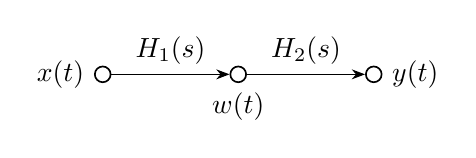
\begin{tikzpicture}[auto, >=Stealth, node distance=1.5cm]
            \tikzset{signode/.style={circle, draw, minimum size=2mm, inner sep=0pt, line width=0.6pt}}
            \node[signode, label=left:$x(t)$] (x) {};
            \node[signode, right=of x, label=below:$w(t)$] (w) {};
            \node[signode, right=of w, label=right:$y(t)$] (y) {};
            \draw[->] (x) -- node {$H_1(s)$} (w);
            \draw[->] (w) -- node {$H_2(s)$} (y);
        \end{tikzpicture}
        \caption{串联}
    \end{minipage}
    \hfill
    \begin{minipage}{0.45\textwidth}
        \centering
        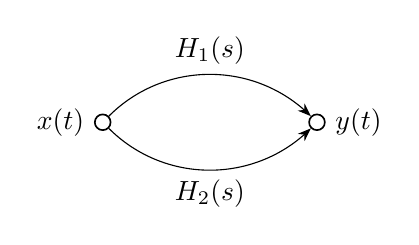
\begin{tikzpicture}[auto, >=Stealth, node distance=2.5cm]
            \tikzset{signode/.style={circle, draw, minimum size=2mm, inner sep=0pt, line width=0.6pt}}
            \node[signode, label=left:$x(t)$] (x) {};
            \node[signode, right=of x, label=right:$y(t)$] (y) {};
            \draw[->] (x) to[bend left=45] node {$H_1(s)$} (y);
            \draw[->] (x) to[bend right=45] node[swap] {$H_2(s)$} (y);
        \end{tikzpicture}
        \caption{并联}
    \end{minipage}
\end{figure}

此外，还可以引入反馈回路，根据是否有反馈回路，系统分为开环系统和闭环系统。
\begin{definition}[开环系统与闭环系统]
    如果系统取后级响应为反馈信号输入到前级，则该系统称为\textbf{闭环系统}，否则称为\textbf{开环系统}。
\end{definition}

\begin{figure}[H]
    \centering
    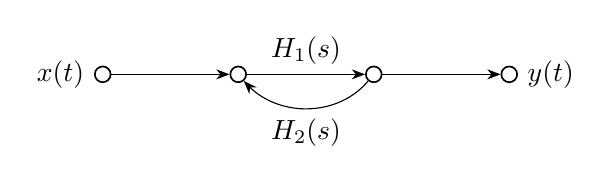
\begin{tikzpicture}[auto, >=Stealth, node distance=1.5cm]
        \tikzset{signode/.style={circle, draw, minimum size=2mm, inner sep=0pt, line width=0.6pt}}
        
        \node[signode, label=left:$x(t)$] (x) {};
        \node[signode, right=of x] (e) {};
        \node[signode, right=of e] (pre_y) {};
        \node[signode, right=of pre_y, label=right:$y(t)$] (y) {};
        
        \draw[->] (x) -- (e);
        \draw[->] (e) -- node {$H_1(s)$} (pre_y);
        \draw[->] (pre_y) -- (y);
        \draw[->] (pre_y) to[bend left=50] node {$H_2(s)$} (e);
    \end{tikzpicture}
    \caption{闭环系统}
\end{figure}

上图展示了一个最简单的闭环系统的信号流图。我们将$H_1(s)$称为\textbf{开环增益}，表示不考虑反馈回路时系统的增益，与之相对，将考虑反馈回路后的增益称为\textbf{闭环增益}。

计算该系统的闭环增益：
\begin{align*}
    Y(s)&=H_1(s)E(s)\\
    E(s)&=X(s)-H_2(s)Y(s)\\
    \implies Y(s)&=H_1(s)\left[X(s)-H_2(s)Y(s)\right]\\
    \implies Y(s)&=\frac{H_1(s)}{1+H_1(s)H_2(s)}X(s)\\
    \implies H(s)&=\frac{Y(s)}{X(s)}=\frac{H_1(s)}{1+H_1(s)H_2(s)}
\end{align*}

\begin{definition}[反馈深度与反馈类型]
将$1+H_1(s)H_2(s)$称为\textbf{反馈深度}，它是引入反馈回路导致的增益下降的倍率。

如果反馈深度大于1，则系统的输出更加稳定，但增益下降，此时反馈为\textbf{负反馈}，特别地，如果反馈深度远大于1，称为\textbf{深度负反馈}，此时$1+H_1(s)H_2(s)\approx H_1(s)H_2(s)$，增益近似等于$1/H_2(s)$（即反馈回路系统的逆系统），与开环增益无关。

如果反馈深度小于1，则系统的输出不稳定，但增益变高，称为\textbf{正反馈}，多用于振荡器；如果反馈深度近似为0，系统将进入\textbf{自激振荡状态}，通常电路无法正常工作，需要消除这种状态。
\end{definition}

\begin{example}
    设$X_1,X_2$为输入节点，$Y_1,Y_2$为输出节点，其他节点为混合节点。
    \begin{figure}[H]
        \centering
        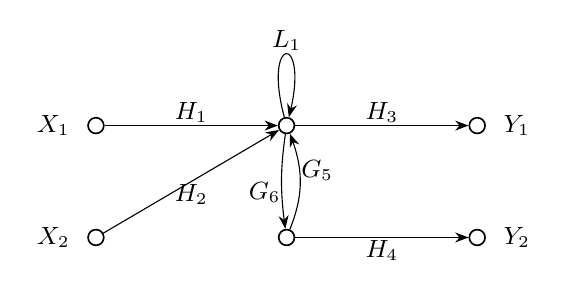
\begin{tikzpicture}[auto, >=Stealth, node distance=1.8cm, every node/.style={font=\small}]
            % node styles: hollow smaller circles
            \tikzset{
                signode/.style={circle, draw, minimum size=2mm, inner sep=0pt, line width=0.6pt},
                lab/.style={font=\small}
            }
            % nodes (empty hollow circles)
            \node[signode] (x1) {};
            \node[signode, below=1.2cm of x1] (x2) {};
            \node[signode, right=2.2cm of x1] (m1) {};
            \node[signode, right=2.2cm of x2] (m2) {};
            \node[signode, right=2.2cm of m1] (y1) {};
            \node[signode, right=2.2cm of m2] (y2) {};
            % external labels (placed to avoid overlap)
            \node[lab, left=1mm of x1] {$X_1$};
            \node[lab, left=1mm of x2] {$X_2$};
            \node[lab, right=1mm of y1] {$Y_1$};
            \node[lab, right=1mm of y2] {$Y_2$};
            % forward path gains use H_i, feedback/return gains use G_j
            \draw[->] (x1) to node[midway, above,  inner sep=1pt] {$H_1$} (m1);
            \draw[->] (x2) to node[midway, below,  inner sep=1pt] {$H_2$} (m1);
            \draw[->] (m1) to node[midway, above,  inner sep=1pt] {$H_3$} (y1);
            \draw[->] (m2) to node[midway, below,  inner sep=1pt] {$H_4$} (y2);
            % adjusted label positions for G_5 and G_6 to avoid overlap
            \draw[->] (m1) to[bend right=8] node[midway, right,xshift=6pt, yshift=4pt,  inner sep=1pt] {$G_5$} (m2);
            \draw[->] (m2) to[bend right=22] node[midway, left, xshift=-6pt,yshift=-4pt,  inner sep=1pt] {$G_6$} (m1);
            \draw[->] (m1) edge[loop above, looseness=50] node[  inner sep=1pt] {$L_1$} (m1);
        \end{tikzpicture}
    \end{figure}
    记上、下两个混合节点对应的中间变量分别为$M_1,M_2$，则
    \begin{align*}
        M_1&=H_1 X_1+H_2 X_2+L_1 M_1+G_5 M_2\\
        M_2&=G_6 M_1\\
        Y_1&=H_3 M_1\\
        Y_2&=H_4 M_2
    \end{align*}
    这是一个以$M_1,M_2,Y_1,Y_2$为未知数的线性方程组，可以解得\begin{align*}
        M_1&=\frac{H_1 X_1+H_2 X_2}{1-L_1-G_5 G_6}\\
        M_2&=\frac{G_6 (H_1 X_1+H_2 X_2)}{1-L_1-G_5 G_6}\\
        Y_1&=\frac{H_3 (H_1 X_1+H_2 X_2)}{1-L_1-G_5 G_6}\\
        Y_2&=\frac{H_4 G_6 (H_1 X_1+H_2 X_2)}{1-L_1-G_5 G_6}
    \end{align*}
\end{example}

信号流图是一种有向图，$n$个节点的信号流图可以通过$n$阶的\textbf{邻接矩阵}$A$来表示，其元素$a_{ij}$表示从节点$j$到节点$\mathrm{i}$的支路增益，如果没有支路连接这两个节点，则$a_{ij}=0$。%显然，信号流图可由其邻接矩阵唯一表示，但邻接矩阵中会有一些冗余的行和列。我们通过一个例子来说明这一点。

\begin{example}
    上例中，节点依次为$X_1,X_2,M_1,M_2,Y_1,Y_2$，则对应的邻接矩阵为
    \[A= \begin{bmatrix}
        0 & 0 & 0 & 0 & 0 & 0 \\
        0 & 0 & 0 & 0 & 0 & 0 \\
        H_1 & H_2 & L_1 & G_5 & 0 & 0 \\
        0 & 0 & G_6 & 0 & 0 & 0 \\
        0 & 0 & H_3 & 0 & 0 & 0 \\
        0 & 0 & 0 & H_4 & 0 & 0
    \end{bmatrix}\]
    在信号流图的语境下，源点对应的行和阱点对应的列均为0。有冗余的行和列，不是我们希望看到的。

    事实上，我们仅仅需要中间节点对应的邻接矩阵。由于响应$Y_1,Y_2$直接取自中间节点，只需要求解$M_1,M_2$，就可获取系统的全部信息。将信号流图表示为一个线性方程组：
    \[\begin{bmatrix}
        M_1 \\
        M_2
    \end{bmatrix}=
    \begin{bmatrix}
        L_1 & G_5\\
        G_6 & 0
    \end{bmatrix}
    \begin{bmatrix}
        M_1 \\
        M_2
    \end{bmatrix}+\begin{bmatrix}
        H_1 X_1 + H_2 X_2 \\
        0
    \end{bmatrix},\text{即}\mathbf{M}=A\mathbf{M}+\mathbf{X}\]
    其中$$A=\begin{bmatrix}
        L_1 & G_5\\
        G_6 & 0
    \end{bmatrix}\text{为中间节点的邻接矩阵},\mathbf{M}=\begin{bmatrix}
        M_1 \\
        M_2
    \end{bmatrix},\mathbf{X}=\begin{bmatrix}
        H_1 X_1 + H_2 X_2 \\
        0
    \end{bmatrix}$$
    整理得\[\begin{bmatrix}
        H_1 X_1 + H_2 X_2 \\
        0
    \end{bmatrix}=\begin{bmatrix}
        1 -L_1 & -G_5\\
        -G_6 & 1
    \end{bmatrix}\begin{bmatrix}
        M_1 \\
        M_2
    \end{bmatrix},\text{即}\mathbf{X}=(I-A)\mathbf{M}\]
    只要矩阵\[S=I-A=\begin{bmatrix}
        1 -L_1 & -G_5\\
        -G_6 & 1
    \end{bmatrix}\]
    可逆，就可以求解出$M_1,M_2$，我们将这个矩阵称为\textbf{系统矩阵}(system matrix)，而将$A$称为\textbf{增益矩阵}。系统矩阵的行列式称为\textbf{特征行列式}，记为$\Delta$。在本例中，有\begin{align*}
        \Delta&=\begin{vmatrix}
        1 -L_1 & -G_5 \\
        -G_6 & 1
    \end{vmatrix}=1-L_1-G_5 G_6
    \end{align*}
    要使系统稳定，必须有$\Delta=1-L_1-G_5 G_6\neq 0$，否则$M_1,M_2,Y_1,Y_2\to\infty$。
\end{example}

现在来考虑更一般的情况：对于有n个中间节点$M_1,M_2,\cdots,M_n$的系统，不妨设激励接入的节点为$M_1$（否则可用叠加原理单独分析各个激励），则系统对应的线性方程组为\begin{align*}
    M_1&=a_{11} M_1 + a_{12} M_2 + \cdots + a_{1n} M_n + X\\
    M_2&=a_{21} M_1 + a_{22} M_2 + \cdots + a_{2n} M_n\\
    &\vdots\\
    M_n&=a_{n1} M_1 + a_{n2} M_2 + \cdots + a_{nn} M_n
\end{align*}
写成矩阵形式为
\[\mathbf{M}=A\mathbf{M}+\mathbf{X}\]
其中$$\mathbf{M}=\begin{bmatrix}
    M_1 \\
    M_2 \\
    \vdots \\
    M_n
\end{bmatrix},\mathbf{X}=\begin{bmatrix}
    X \\
    0 \\
    \vdots \\
    0
\end{bmatrix}$$
在系统矩阵$S=I-A$可逆时，有
\[\mathbf{M}=(I-A)^{-1}\mathbf{X}=S^{-1}\mathbf{X}\]
因此中间节点$M_i$可由以下公式计算：\[M_i=\frac{S^*_{1i}}{\Delta} X\]
其中$\Delta=\det S$为特征行列式，$S^*_{1i}$为系统矩阵$S$的去掉第1行、第i列所得的代数余子式。输出节点的响应是中间节点线性组合。以$M_n$为输出为例（否则可更换节点命名并重复此过程），可以写出\textbf{梅森增益公式}(Mason gain formula)：
\begin{theorem}[梅森增益公式]
    设系统有$n$个中间节点$M_1,M_2,\cdots,M_n$，激励$X$接入节点$M_1$，响应$Y$取自节点$M_n$，则
    \[H=\frac{Y}{X}=(S^{-1})_{1n}=\frac{S^*_{n1}}{\Delta}\]
    其中$(S^{-1})_{1n}$为系统矩阵$S$的逆矩阵的第1行第$n$列元素，$\Delta=\det S$为特征行列式，$S^*_{n1}$为系统矩阵$S$的去掉第$n$行、第1列所得的代数余子式。
\end{theorem}

根据行列式的图论展开的几何意义，梅森增益公式又可以写成如下形式：
\begin{theorem}[梅森增益公式，图论形式]
    设系统有$n$个中间节点$M_1,M_2,\cdots,M_n$，激励$X$接入节点$M_1$，响应$Y$取自节点$M_n$，则
    \[H=\frac{Y}{X}=\frac{\sum_{k}g_k\Delta_k}{\Delta}\]
    其中$g_k$为从源点到阱点的第$k$条前向通路增益，$\Delta_k$为去掉与第$k$条前向通路接触的所有节点后的特征行列式。

    特征行列式可由以下公式计算：
    $$\Delta=1-\sum_a L_a+\sum_{b,c}L_b L_c-\sum_{d,e,f}L_d L_e L_f+\cdots$$
    其中$\sum_a L_a$表示所有环路增益之和，$\sum_{b,c}L_b L_c$表示所有两两不接触环路增益的乘积之和，$\sum_{d,e,f}L_d L_e L_f$表示所有三者互不接触环路增益的乘积之和，依此类推。
\end{theorem}

下面来解释为什么行列式展开具有几何意义。首先，根据行列式的公式：
\[\det S=\sum_{\sigma\in S_n}\text{sgn}(\sigma)\prod_{i=1}^{n}s_{i,\sigma(i)}\]
其中$S_n$为所有$n$个元素的排列组成的集合，$\text{sgn}(\sigma)$为排列$\sigma$的符号。对于$S=I-A$，对角元为$s_{ii}=1-a_{ii}$，非对角元为$s_{ij}=-a_{ij}$。

我们知道，每个置换都可以分解为不相交循环的乘积，例如，$$\sigma(1)=3,\sigma(3)=4,\sigma(4)=1,\sigma(2)=5,\sigma(5)=2$$
可以表示为
$$\sigma=(1\ 3\ 4)(2\ 5)$$
对应中间节点组成的环路
$$M_1\to M_3\to M_4\to M_1,M_2\to M_5\to M_2$$
因此，行列式的每一项$\prod_{i=1}^{n}s_{i,\sigma(i)}$都可以看作是由若干个不接触环路增益的乘积。如果环路中出现不动点$\sigma(\mathrm{i})=\mathrm{i}$，则对应的$s_{ii}=1-a_{ii}$中的1，表示该节点不参与任何环路；如果考虑自环，则对应$-a_{ii}$。

其次，考虑正负号的问题。对于k-循环，它对$\text{sgn}(\sigma)$的贡献为$(-1)^{k-1}$，而每个增益对应一个$-a_{ij}$，因此k-循环对行列式的贡献为$(-1)^{k-1}(-1)^k=-1$。因此，$l$个互不接触的环路增益之积的符号应为$(-1)^l$。
\begin{example}
    考虑具有六个中间节点的信号流图，我们来计算$\sigma=(1)(2)(3\ 4\ 5\ 6)$对应的行列式项：
    \[\text{sgn}(\sigma)\prod_{i=1}^{6}s_{i,\sigma(i)}=s_{1,1}s_{2,2}s_{3,4}s_{4,5}s_{5,6}s_{6,3}=(1-a_{11})(1-a_{22})a_{34}a_{45}a_{56}a_{63}\]
    将因式$(1-a_{11})(1-a_{22})$展开，得到
    \[a_{34}a_{45}a_{56}a_{63}-a_{11}\cdot a_{34}a_{45}a_{56}a_{63}-a_{22}\cdot a_{34}a_{45}a_{56}a_{63}+a_{11}\cdot a_{22}\cdot a_{34}a_{45}a_{56}a_{63}\]
    记环路$L:M_3\to M_4\to M_5\to M_6\to M_3$，这四项分别对应以下四种情况：\begin{itemize}
        \item 不考虑节点$M_1,M_2$的自环，仅考虑环路L，符号为$-1$；
        \item 不考虑节点$M_2$的自环，考虑节点$M_1$的自环以及环路L，符号为$+1$；
        \item 不考虑节点$M_1$的自环，考虑节点$M_2$的自环以及环路L，符号为$+1$；
        \item 考虑节点$M_1,M_2$的自环以及环路L，符号为$-1$。
    \end{itemize}
\end{example}

最后，对于代数余子式$S^*_{n1}=\sum_{k}g_k\Delta_k$，我们考虑将$S$按第$n$行展开：
\[\det S=\Delta=\sum_{j=1}^{n}s_{nj}S^*_{nj}\]
这样，$S^*_{n1}$就对应$s_{n1}$的系数。行列式公式中某一项包含$s_{n1}$，说明置换$\sigma$中有$\sigma(1)=n$，即环路包含$M_1\to M_n$。将该环路的其余部分补全，就得到了一条从$M_1$到$M_n$的前向通路，其前向通路增益为$g_k$。去掉与该环路接触的节点后，剩下的部分正好对应$\Delta_k$。

注意，如果原图中不含有$M_1\to M_n$的支路，则$s_{n1}=0$，此时我们只好假想有一条“增益为0”的支路连接$M_1$和$M_n$，才能看出代数余子式的几何意义。因此，在梅森增益公式中，我们总是需要将前向通路考虑进来，而不管是否存在$M_1\to M_n$的支路。

\begin{example}
    考虑具有4个中间节点的信号流图：
    \begin{figure}[H]
        \centering
        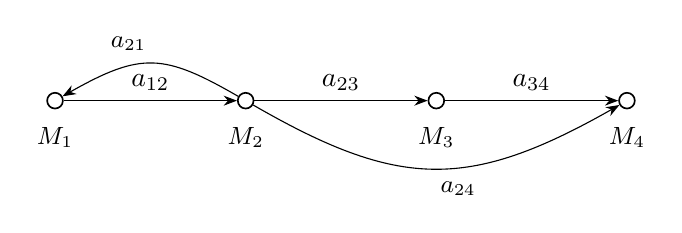
\begin{tikzpicture}[auto, >=Stealth, node distance=2.2cm]
            % 节点（2mm空心小圆）
            \node[circle, draw, minimum size=2mm, inner sep=0pt, line width=0.6pt] (M1) {};
            \node[circle, draw, minimum size=2mm, inner sep=0pt, line width=0.6pt, right=of M1] (M2) {};
            \node[circle, draw, minimum size=2mm, inner sep=0pt, line width=0.6pt, right=of M2] (M3) {};
            \node[circle, draw, minimum size=2mm, inner sep=0pt, line width=0.6pt, right=of M3] (M4) {};
            % 节点标记，避免重叠
            \node[font=\small, below=3pt of M1] {$M_1$};
            \node[font=\small, below=3pt of M2] {$M_2$};
            \node[font=\small, below=3pt of M3] {$M_3$};
            \node[font=\small, below=3pt of M4] {$M_4$};
            % 边
            \draw[->] (M1) -- node[midway, above] {$a_{12}$} (M2);
            \draw[->] (M2) -- node[midway, above] {$a_{23}$} (M3);
            % a_{24}弯曲到M4
            \draw[->] (M2) to[out=-30,in=210,looseness=1.2] node[below right=1pt and -2pt, font=\small] {$a_{24}$} (M4);
            \draw[->] (M3) -- node[midway, above] {$a_{34}$} (M4);
            % a_{21}反馈支路弯曲
            \draw[->] (M2) to[out=150,in=30,looseness=1.3] node[above left=1pt and -2pt, font=\small] {$a_{21}$} (M1);
        \end{tikzpicture}
    \end{figure}
    仍设激励接入的节点为$M_1$，输出取自节点$M_n$，则前向通路有两条：
    \[M_1\to M_2\to M_3\to M_4,M_1\to M_2\to M_4\]
    我们来考察前向通路与系统矩阵的对应关系。增益矩阵为
    \[A=\begin{bmatrix}
        0 & a_{12} & 0 & 0 \\
        a_{21} & 0 & a_{23} & a_{24} \\
        0 & 0 & 0 & a_{34} \\
        0 & 0 & 0 & 0
    \end{bmatrix}\]
    因此系统矩阵为
    \[S=I-A=\begin{bmatrix}
        1 & s_{12} & 0 & 0 \\
        s_{21} & 1 & s_{23} & s_{24} \\
        0 & 0 & 1 & s_{34} \\
        0 & 0 & 0 & 1
    \end{bmatrix}\]
    
    这个系统并没有$M_4\to M_1$的支路，但我们假想有支路$a_{41}=-s_{41}=0$，这样就产生了环路
    $$M_1\to M_2\to M_3\to M_4\to M_1,M_1\to M_2\to M_4\to M_1$$
    前向通路增益分别为$g_1=a_{12}a_{23}a_{34}$和$g_2=a_{12}a_{24}$。

    计算特征行列式：原图中有环路$M_1\to M_2\to M_1$，环路增益为$L_1=a_{12}a_{21}$，特征行列式为$\Delta=1-L_1=1-a_{12}a_{21}$；对于两条前向通路，去掉所涉及的节点后不再有回路，因此$\Delta_1=\Delta_2=1$。根据梅森增益公式，有
    \[H=\frac{Y}{X}=\frac{g_1\Delta_1+g_2\Delta_2}{\Delta}=\frac{a_{12}a_{23}a_{34}+a_{12}a_{24}}{1-a_{12}a_{21}}\]
\end{example}

一般来说，我们直接用计算机分析信号流图表示的复杂系统，但在一些特定的信号流图中，使用几何意义更为方便。

\begin{example}[单入单出信号流图]
    系统的信号流图如图所示：
    \begin{figure}[H]
        \centering
        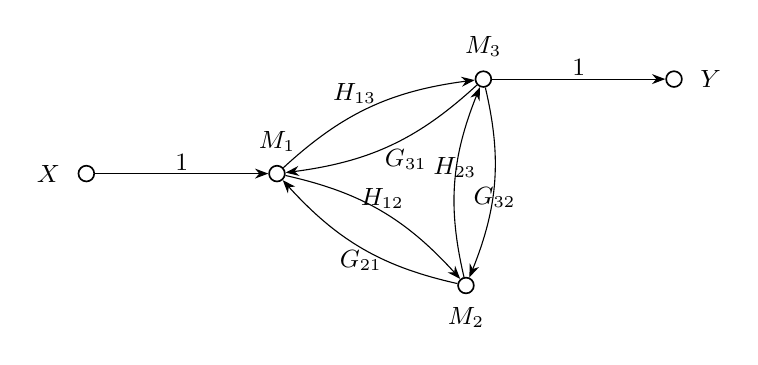
\begin{tikzpicture}[auto, >=Stealth, node distance=1.8cm, every node/.style={font=\small}]
            \tikzset{signode/.style={circle, draw, minimum size=2mm, inner sep=0pt, line width=0.6pt}, lab/.style={font=\small}}
            % nodes
            \node[signode] (X) {};
            \node[signode, right=2.2cm of X] (m1) {};
            \node[signode, below=1.2cm of m1,xshift=24mm] (m2) {};
            \node[signode, right=2.4cm of m1, yshift=12mm] (m3) {};
            \node[signode, right=2.2cm of m3] (Y) {}; 
            % labels
            \node[lab,left=1mm of X] {$X$};
            \node[lab,right=1mm of Y] {$Y$};
            \node[lab, above=0.5mm of m1] {$M_1$};
            \node[lab, below=0.5mm of m2] {$M_2$};
            \node[lab, above=0.5mm of m3] {$M_3$};
            % input connects only to m1 with unit gain
            \draw[->] (X) to node[midway, above, inner sep=1pt] {$1$} (m1);
            % output is taken from m3 with unit gain
            \draw[->] (m3) to node[midway, above, inner sep=1pt] {$1$} (Y);
            % complete directed subgraph among m1..m3 (H_ij for forward, G_ij for feedback)
            \draw[->] (m1) to[bend left=18] node[midway, above, inner sep=1pt] {$H_{12}$} (m2);
            \draw[->] (m2) to[bend left=18] node[midway, below, inner sep=1pt] {$G_{21}$} (m1);
            \draw[->] (m1) to[bend left=18] node[midway, above, inner sep=1pt,xshift=-6pt] {$H_{13}$} (m3);
            \draw[->] (m3) to[bend left=18] node[midway, below, inner sep=1pt,xshift=6pt] {$G_{31}$} (m1);
            \draw[->] (m2) to[bend left=18] node[midway, above, inner sep=1pt] {$H_{23}$} (m3);
            \draw[->] (m3) to[bend left=18] node[midway, below, inner sep=1pt] {$G_{32}$} (m2);
        \end{tikzpicture}
    \end{figure}
    \ding{172}使用矩阵进行分析：系统矩阵为
    \[\begin{bmatrix}
        1 & -G_{21} & -G_{31} \\
        -H_{12} & 1 & -G_{32} \\
        -H_{13} & -H_{23} & 1
    \end{bmatrix}\]
    特征行列式为
    $$\Delta=\begin{vmatrix}
        1 & -G_{21} & -G_{31} \\
        -H_{12} & 1 & -G_{32} \\
        -H_{13} & -H_{23} & 1
    \end{vmatrix}=1-G_{21}H_{12}-G_{31}H_{13}-G_{32}H_{23}-G_{21}G_{32}H_{13}-G_{31}H_{23}H_{12}$$
    在$\Delta\neq 0$时，系统矩阵可逆，其逆矩阵为\begin{align*}
        S^{-1}=\frac{1}{\Delta}\begin{bmatrix}
            1-G_{32}H_{23} & G_{21}+G_{31}H_{23} & G_{31}+G_{21}G_{32} \\
            H_{12}+H_{13}G_{32} & 1-G_{31}H_{13} & G_{32}+G_{31}H_{12} \\
            H_{13}+H_{12}H_{23} & H_{23}+G_{21}H_{13} & 1-G_{21}H_{12}
        \end{bmatrix}
    \end{align*}
    输出为$Y=M_3=\frac{1}{\Delta}(H_{13}+H_{12}H_{23})X$，因此系统增益为
    \[H=\frac{Y}{X}=\frac{H_{13}+H_{12}H_{23}}{\Delta}=\frac{H_{13}+H_{12}H_{23}}{1-G_{21}H_{12}-G_{31}H_{13}-G_{32}H_{23}-G_{21}G_{32}H_{13}-G_{31}H_{23}H_{12}}\]

    \ding{173}使用梅森增益公式的几何意义：图中共有五个环路，分别为\begin{align*}
        L_1&:M_1\to M_2\to M_1,\text{增益}L_1=G_{21}H_{12}\\
        L_2&:M_1\to M_3\to M_1,\text{增益}L_2=G_{31}H_{13}\\
        L_3&:M_2\to M_3\to M_2,\text{增益}L_3=G_{32}H_{23}\\
        L_4&:M_1\to M_2\to M_3\to M_1,\text{增益}L_4=G_{21}G_{32}H_{13}\\
        L_5&:M_1\to M_3\to M_2\to M_1,\text{增益}L_5=G_{31}H_{23}H_{12}
    \end{align*}
    这五个环路两两相交，因此特征行列式为
    \[\Delta=1-(L_1+L_2+L_3+L_4+L_5)=1-G_{21}H_{12}-G_{31}H_{13}-G_{32}H_{23}-G_{21}G_{32}H_{13}-G_{31}H_{23}H_{12}\]
    前向通路共有两条，增益分别为$g_1=H_{13}$和$g_2=H_{12}H_{23}$，去掉前向通路中的节点后没有环路，因此$\Delta_1=\Delta_2=1$。根据梅森增益公式，有
    \[H=\frac{g_1\Delta_1+g_2\Delta_2}{\Delta}=\frac{H_{13}+H_{12}H_{23}}{1-G_{21}H_{12}-G_{31}H_{13}-G_{32}H_{23}-G_{21}G_{32}H_{13}-G_{31}H_{23}H_{12}}\]
\end{example}

我们同样能够根据系统函数画出信号流图，但是一个的系统函数可以对应多种信号流图，例如两个系统的级联是可交换的。下面给出一种仅仅使用乘法器和积分器（系统函数为$s^{-1}$）将有理系统函数化为信号流图的标准方法，使用这种方法画出的信号流图是唯一的，并且具有相似的结构。

考虑如下信号流图：

\begin{center}
\scalebox{0.92}{%
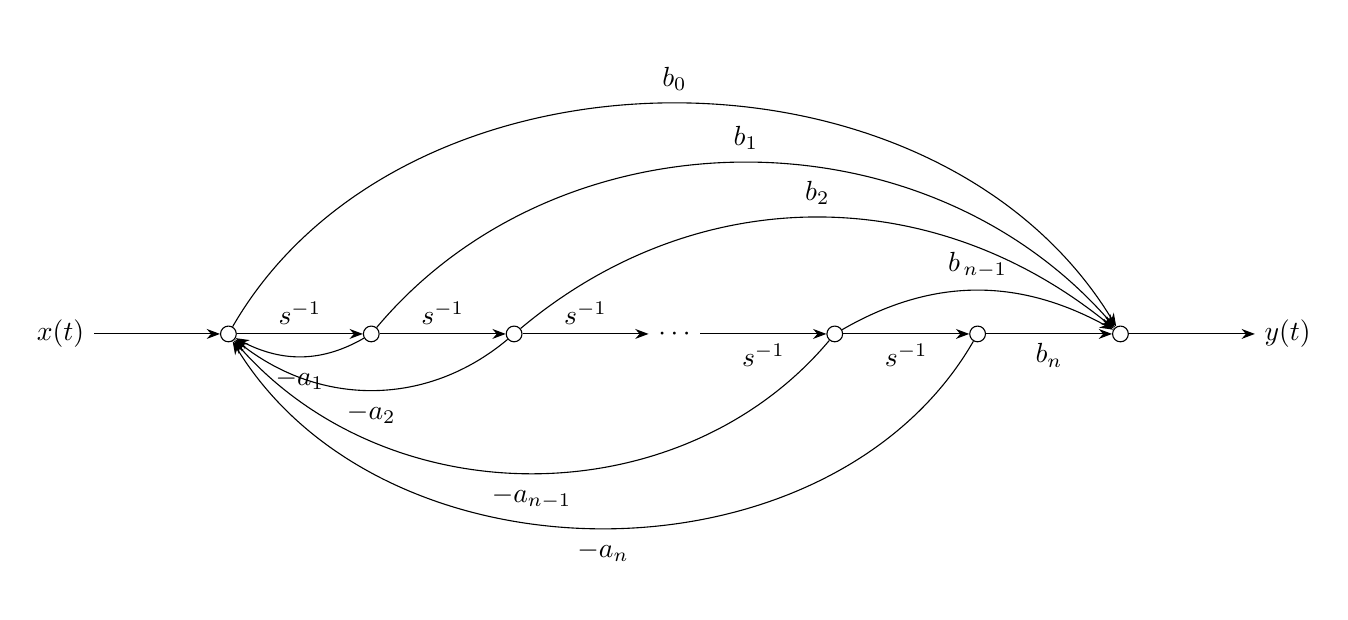
\begin{tikzpicture}[>=Stealth, node distance=1.6cm, auto]
    % 节点：M1 为矩形，其余中间节点用直径为2的小圆圈表示，节点内部不显示编号
    \node (x) {$x(t)$};
    \node[draw, circle, minimum size=2mm, inner sep=0pt] (M1) [right=of x] {};
    \node[circle, draw, minimum size=2mm, inner sep=0pt] (M2) [right=of M1] {};
    \node[circle, draw, minimum size=2mm, inner sep=0pt] (M3) [right=of M2] {};
    \node (dots) [right=of M3] {$\cdots$};
    \node[circle, draw, minimum size=2mm, inner sep=0pt] (Mn_2) [right=of dots] {};
    \node[circle, draw, minimum size=2mm, inner sep=0pt] (Mn_1) [right=of Mn_2] {};
    \node[circle, draw, minimum size=2mm, inner sep=0pt] (Mn) [right=of Mn_1] {};
    \node (y) [right=of Mn] {$y(t)$};

    % 串联 s^{-1} 通路（链路上方标注，避免与其他箭头重叠）
    \draw[->] (x) -- (M1);
    \draw[->] (M1) -- node[above] {$s^{-1}$} (M2);
    \draw[->] (M2) -- node[above] {$s^{-1}$} (M3);
    \draw[->] (M3) -- node[above] {$s^{-1}$} (dots);
    \draw[->] (dots) -- node[below] {$s^{-1}$} (Mn_2);
    \draw[->] (Mn_2) -- node[below] {$s^{-1}$} (Mn_1);
    \draw[->] (Mn_1) -- node[below] {$b_n$} (Mn);
    \draw[->] (Mn) -- (y);

    % 直接到 Mn 的前向通路，标签放在上方并调整弯度避免重叠
    \draw[->, bend left=60] (M1) to node[above, yshift=1pt] {$b_0$} (Mn);
    \draw[->, bend left=50] (M2) to node[above, yshift=1pt] {$b_1$} (Mn);
    \draw[->, bend left=40] (M3) to node[above, yshift=1pt] {$b_2$} (Mn);
    \draw[->, bend left=30] (Mn_2) to node[above, yshift=1pt] {$b_{\,n-1}$} (Mn);

    % 反馈回到 M1（画在下方，标签置于弧线下方并微调，避免文字与箭头相交）
    \draw[->, bend left=30] (M2) to node[below, yshift=-1pt] {$-a_1$} (M1);
    \draw[->, bend left=40] (M3) to node[below, yshift=-1pt] {$-a_2$} (M1);
    \draw[->, bend left=50] (Mn_2) to node[below, yshift=-1pt] {$-a_{n-1}$} (M1);
    \draw[->, bend left=60] (Mn_1) to node[below, yshift=-1pt] {$-a_{n}$} (M1);
\end{tikzpicture}%
}
\end{center}

注意到这个信号流图的所有前向通路和环路均经过节点$M_1$，去掉节点$M_1$后不再有环路，因此不含$M_1$的子图的特征行列式$\Delta_k$均为1。利用梅森增益公式，可以计算出系统增益为
\begin{align*}
    H(s)&=\frac{Y(s)}{X(s)}=\frac{b_0 + b_1 s^{-1} + b_2 s^{-2} + \cdots + b_n s^{-n}}{1 + a_1 s^{-1} + a_2 s^{-2} + \cdots + a_n s^{-n}}
\end{align*}

可见，对于任意有理系统函数，都可以使用上述信号流图表示。注意系数$a_k,b_k$是可以为0的，因此即便分子分母不是相同度数的多项式，也可以使用该信号流图表示。

\subsection{最小相位系统}\label{sub:min_phase}

根据\ref{sub:stability_of_system}，对于因果且稳定的连续线性时不变系统，系统函数$H(s)$的所有极点均位于复平面的左半平面。如果我们还希望系统具有最小的相位延迟特性，从而具有最小的时延特性，则需要系统函数$H(s)$的所有零点也位于复平面的左半平面，这样的系统称为\textbf{最小相位系统}(minimum-phase system)。

\begin{definition}[最小相位系统]
    设因果且稳定的连续线性时不变系统的系统函数为$H(s)$，记$H(s)$的零点集为$\{z_k\}$，如果$\forall k,\text{Re}(z_k)<0$，则称该系统为\textbf{最小相位系统}。
\end{definition}

为了说明为什么这样的系统具有最小的延时特性，我们首先考虑一个例子：
\begin{example}
    设因果且稳定的连续线性时不变系统A，B的系统函数分别为
    \[H_A(s)=\frac{s+1}{s+2},H_B(s)=\frac{s-1}{s+2}\]
    这两个系统具有相同的幅频特性：
    \[|H_A(\mathrm{i}\omega)|=|H_B(\mathrm{i}\omega)|=\frac{\sqrt{\omega^2+1}}{\sqrt{\omega^2+4}}\]
    其中系统A为最小相位系统，系统B不是最小相位系统。计算两个系统的相频特性：
    \begin{align*}
        \varphi_A(\omega)&=\arg(\mathrm{i}\omega+1)-\arg(\mathrm{i}\omega+2)=\arctan(\omega)-\arctan\left(\frac{\omega}{2}\right)\\
        \varphi_B(\omega)&=\arg(\mathrm{i}\omega-1)-\arg(\mathrm{i}\omega+2)=-\arctan(\omega)-\arctan\left(\frac{\omega}{2}\right)
    \end{align*}

    在\ref{sub:distortion}中曾介绍，考察系统的延时特性，可以使用相时延$\tau_p$和群时延$\tau_g$。计算两个系统的相时延和群时延：
    \begin{align*}
        \tau_{pA}(\omega)&=-\frac{\varphi_A(\omega)}{\omega}=\frac{-\arctan(\omega)+\arctan\left(\frac{\omega}{2}\right)}{\omega}\\
        \tau_{pB}(\omega)&=-\frac{\varphi_B(\omega)}{\omega}=\frac{\arctan(\omega)+\arctan\left(\frac{\omega}{2}\right)}{\omega}\\
        \tau_{gA}(\omega)&=-\frac{d\varphi_A(\omega)}{d\omega}=-\frac{1}{1+\omega^2}+\frac{2}{4+\omega^2}\\
        \tau_{gB}(\omega)&=-\frac{d\varphi_B(\omega)}{d\omega}=\frac{1}{1+\omega^2}+\frac{2}{4+\omega^2}
    \end{align*}
    可以发现，
    \begin{align*}
        &\tau_{pA}(\omega)-\tau_{pB}(\omega)=-\frac{2\arctan(\omega)}{\omega}<0\\
        &\tau_{gA}(\omega)-\tau_{gB}(\omega)=-\frac{2}{1+\omega^2}<0
    \end{align*}
    也就是说，最小相位系统A的相时延和群时延均小于非最小相位系统B的相时延和群时延，因此系统A具有更好的延时特性。
\end{example}

\begin{proposition}
    具有相同幅频特性的因果且稳定的连续线性时不变系统中，最小相位系统具有最小的相时延和群时延，因此具有最佳的延时特性。
\end{proposition}
\begin{proof}
    我们对系统函数为有理函数的情况进行证明。设因果且稳定的连续线性时不变系统的系统函数为
    \[H(s)=K(s)\frac{\prod_{k=1}^{m}(s-z_k)}{\prod_{l=1}^{n}(s-p_l)}\]
    其中$K(s)$仅有左半平面内的零点而没有极点。$\text{Re}(p_l)<0,\forall l,\text{Re}(z_k)> 0,\forall k$。设系统函数$H(s)$的幅频特性为$|H(\mathrm{i}\omega)|=A(\omega)$，则
    \[A(\omega)=|K(s)|\frac{\prod_{k=1}^{m}\sqrt{\omega^2+|z_k|^2}}{\prod_{l=1}^{n}\sqrt{\omega^2+|p_l|^2}}\]
    设另一个系统的系统函数为
    \[\tilde{H}(s)=K(s)\frac{\prod_{k=1}^{m}(s-\tilde{z}_k)}{\prod_{l=1}^{n}(s-p_l)}\]
    其中$\tilde{z}_k=-\overline{z_k}$，即$z_k$关于虚轴的对称点，则$\tilde{H}(s)$的幅频特性与$H(s)$相同，且该系统是最小相位系统。计算两个系统的相频特性之差：
    \begin{align*}
        \varphi(\omega)-\tilde{\varphi}(\omega)&=\sum_{k=1}^{m}\left(\arg(\mathrm{i}\omega-z_k)-\arg(\mathrm{i}\omega-\tilde{z}_k)\right)\\
        &=\sum_{k=1}^{m}\left(\arctan\left(\frac{\omega-\text{Im}(z_k)}{-\text{Re}(z_k)}\right)-\arctan\left(\frac{\omega-\text{Im}(z_k)}{\text{Re}(z_k)}\right)\right)\\
        &=-2\sum_{k=1}^{m}\arctan\left(\frac{\omega-\text{Im}(z_k)}{\text{Re}(z_k)}\right)
    \end{align*}
    比较相时延和群时延：
    \begin{align*}
        \tau_p(\omega)-\tilde{\tau}_p(\omega)&=-\frac{\varphi(\omega)-\tilde{\varphi}(\omega)}{\omega}\\
        &=\frac{2}{\omega}\sum_{k=1}^{m}\arctan\left(\frac{\omega-\text{Im}(z_k)}{\text{Re}(z_k)}\right)>0\\
        \tau_g(\omega)-\tilde{\tau}_g(\omega)&=-\frac{d}{d\omega}(\varphi(\omega)-\tilde{\varphi}(\omega))\\
        &=2\sum_{k=1}^{m}\frac{\text{Re}(z_k)}{(\omega-\text{Im}(z_k))^2+\text{Re}(z_k)^2}>0
    \end{align*}
    因此，最小相位系统$\tilde{H}(s)$的相时延和群时延均小于非最小相位系统$H(s)$的相时延和群时延。
\end{proof}

需要指出，这个证明并不严谨。其一，这个证明没有说明为什么最小相位系统要求系统函数在虚轴上也不存在零点；其二，这个证明仅适用于有理函数。但是，更一般的情况需要用到哈代空间中函数的内外分解，我没能找到既严谨又通俗的证明，只能说这个证明能够提供一些直观的理解。

在最小相位系统的约束下，其\textbf{逆系统}也是因果且稳定的连续线性时不变系统。这是因为最小相位系统的系统函数$H(s)$的零点均位于复平面的左半平面，因此其倒数$H^{-1}(s)$的极点也均位于复平面的左半平面，从而保证了逆系统的因果性和稳定性。

\begin{example}
    设因果且稳定的连续线性时不变系统的系统函数及单位脉冲响应为
    \[H(s)=\frac{s+1}{s+2},h(t)=\delta(t)-\mathrm{e}^{-2t}u(t)\]
    则其逆系统的系统函数及单位脉冲响应为
    \[H^{-1}(s)=\frac{s+2}{s+1},h_{inv}(t)=\delta(t)+\mathrm{e}^{-t}u(t)\]
    该逆系统也是因果且稳定的连续线性时不变系统。将两个系统级联，其单位脉冲响应为
\begin{align*}
    h_{eq}(t)&=h(t)*h_{inv}(t)\\
    &=\delta(t)-\mathrm{e}^{-2t}u(t)+\mathrm{e}^{-t}u(t)-(\mathrm{e}^{-2t}u(t))*(\mathrm{e}^{-t}u(t))\\
    &=\delta(t)-\mathrm{e}^{-2t}u(t)+\mathrm{e}^{-t}u(t)-u(t)\int_0^t \mathrm{e}^{-2\tau}\mathrm{e}^{-(t-\tau)}d\tau\\
    &=\delta(t)
\end{align*}
\end{example}

对于逆系统，容易产生这样的误解：将两个系统级联，则系统函数为$H(s)\cdot H^{-1}(s)=1$，因此输出应与输入相同；考虑群时延和相时延，两个系统的群时延和相时延之和必定为0，因此只要两个系统中必有其中之一具有负的时延；进一步，考虑输入单频的正弦信号，在负的相时延下，输出信号应当提前出现，从而违反因果性。

事实上，两个系统都产生时延，与系统在级联后表现为恒等变换系统，二者并不矛盾，并且两个系统也的确满足因果性，上例中已经说明了这一点。

那么，以上“违反因果性”的结论在那一步出错了呢？实际上，这是因为单频正弦信号“提前出现”的表现，并没有破坏因果性，这是因为，当我们考虑系统的激励为正弦信号时，实际上假定这是一个\textbf{稳态}信号，即该正弦信号从$t=-\infty$时刻就已经存在了，我们观察到的相位“提前”，\textbf{实际上是相位延迟}，而级联所得的恒等变换系统总延迟为0，实际上是两个系统的相位延迟相互抵消了。因此，并不存在违反因果性的情况。

进一步，群时延之和为0，表现出调幅信号的包络峰提前出现的现象。这也没有违反因果性，因为响应起始时刻仍在激励之后，这种包络峰提前出现的现象，实际上是\textbf{相位失真引起的波形重构}。

\begin{example}[负的群时延]
    考虑调幅信号通过具有负的群时延的系统。设
    \[e(t)=\cos(\omega_m t)\cos(\omega_c t),H(s)=\frac{s+1}{s+2},h(t)=\delta-\mathrm{e}^{-2t}u(t)\]
    则系统的群时延为
    \[\tau_g(\omega)=-\frac{d\varphi(\omega)}{d\omega}=-\frac{1}{1+\omega^2}+\frac{2}{4+\omega^2}\]
    在低频段，群时延为负值。设基波频率$\omega_m=1$，载波频率$\omega_c=5$（这个载波的频率不算很高，这是为了使响应与激励区分开），则
    \begin{align*}
        e(t)=\cos(t)\cos(5t)=\frac{1}{2}[\cos(4t)+\cos(6t)],\tau_g(1)=-0.1
    \end{align*}
    由此可以预测，系统的响应中，包络峰将提前出现0.1s。

    计算系统的响应：
    \begin{align*}
        y(t)&=(h*e)(t)\\
        &=\cos(t)\cos(5t)-\frac{1}{2}u(t)\int_{0}^{t}\mathrm{e}^{-2\tau}[\cos(4(t-\tau))+\cos(6(t-\tau))]d\tau\\
        &=\cos(t)\cos(5t)-\frac{1}{2}u(t)\left[\frac{\cos(4t)+2\sin(4t)-\mathrm{e}^{-2t}}{10}+\frac{\cos(6t)+3\sin(6t)-\mathrm{e}^{-2t}}{20}\right]
    \end{align*}
    \begin{figure}[H]
        \centering
        \includegraphics[width=0.8\textwidth]{neg_taug}
        \caption{调幅信号通过具有负群时延系统的响应}
    \end{figure}
    上图中，依稀能辨认出-0.1s的群时延，但由于输入的是稳态信号，并没有违反因果性。
\end{example}

那么，对于暂态信号，情况又如何呢？考虑相时延
$$tau_p(\omega)=\dfrac{-\arctan(\omega)+\arctan(\frac{\omega}{2})}{\omega},\forall \omega>0,\tau_p(\omega)<0$$
即各频率分量均有负的相时延。

不过，时限函数不可能同时是带限的（见\ref{sub:time_freq_limit}），激励在全频域上均有频率分量，这当然可能使得响应的各分量提前出现，却在$t=0$时刻前抵消，最终呈现出响应与激励起始时刻相同，不违反因果性的结果。

\begin{example}[暂态信号经过逆系统]
    设
    $$e(t)=\chi_{[0,1]}(t),H(s)=\frac{s+1}{s+2}$$
    则系统的响应为
    \begin{align*}
        y(t)&=(h*\chi_{[0,1]})(t)\\
        &=\chi_{[0,1]}(t)-u(t)\int_0^t \chi_{[0,1]}(\tau)\mathrm{e}^{-2(t-\tau)}d\tau
    \end{align*}
    单位脉冲响应$h(t)$是因果的，因此响应也是因果的。

    在$t<1$时，相应为\begin{align*}
        y(t)&=\chi_{[0,1]}(t)-u(t)\int_0^t \mathrm{e}^{-2(t-\tau)}d\tau\\
        &=\chi_{[0,1]}(t)-\frac{1}{2}u(t)(1-\mathrm{e}^{-2t})
    \end{align*}
    在$t\geq 1$时，相应为\begin{align*}
        y(t)&=\chi_{[0,1]}(t)-u(t)\int_0^1 \mathrm{e}^{-2(t-\tau)}d\tau\\
        &=-\frac{1}{2}u(t)(\mathrm{e}^{-2t}-\mathrm{e}^{-2(t-1)})
    \end{align*}
    \begin{figure}[H]
        \centering
        \includegraphics[width=0.8\textwidth]{inv_system}
        \caption{暂态信号通过逆系统的响应}
    \end{figure}
    响应与激励的起始时刻一致，满足因果性。
\end{example}

\chapter{离散时间变换}

\section{z变换}\label{sec:z_Transform}

\subsection{z变换的引出}\label{sub:inteoduction_of_z}
中学数学中处理递推数列的一种经典方法是使用生成函数，将数列转化为形式幂级数，从而利用级数的性质来分析数列。z变换可以看作生成函数的推广，它将数列推广为离散时间信号,将形式幂级数推广为洛朗级数（我们将在\ref{sub:meromorphic_function}中详细讨论这个洛朗级数的收敛域），从而可以利用复变函数的理论来分析离散时间信号与离散系统。
\begin{definition}[z变换]
    将离散时间信号$x[n]$的z变换记为$X(z)$或$\mathcal{Z} x(z)$，它的定义为
    \[X(z)=\mathcal{Z} x[n]=\sum_{n=-\infty}^{\infty}x[n]z^{-n},z\in\mathbb{C}\]
    我们记$x[n]\overset{\mathcal{Z} }{\longleftrightarrow}X(z)$。
\end{definition}
作为一个洛朗级数，z变换所得函数$X(z)$的收敛域应为一个圆环$\mathcal{A}_0(r,R)$，在圆环内级数是绝对收敛、内闭一致收敛的。根据圆环上全纯函数的洛朗级数的存在性和唯一性，洛朗级数与离散信号一一对应，因此可以使用上面的记号$x[n]\overset{\mathcal{Z} }{\longleftrightarrow}X(z)$。

下面给出一些常用离散信号的z变换作为例子：
\begin{example}[单位脉冲序列的z变换]
    设$x[n]=\delta[n-k],k\in\mathbb{Z}$，则
    \[X(z)=\sum_{n=-\infty}^{\infty}\delta[n-k]z^{-n}=z^{-k},z\in\mathbb{C}\backslash\{0\}\]
\end{example}
\begin{example}[单位阶跃序列的z变换]
    设$x[n]=u[n]$，则
    \[X(z)=\sum_{n=0}^{\infty}z^{-n}=\frac{1}{1-z^{-1}}=\frac{z}{z-1},|z|>1\]
\end{example}
\begin{example}[指数序列的z变换]
    设$x[n]=a^n u[n],a\in\mathbb{C}$，则
    \[X(z)=\sum_{n=0}^{\infty}a^n z^{-n}=\frac{1}{1-a z^{-1}}=\frac{z}{z-a},|z|>|a|\]
\end{example}
\begin{example}[单边余弦序列的z变换]
    \begin{align*}
        \mathcal{Z} \left[\cos(\Omega n)u[n]\right]&=\frac{1}{2}\left(\mathcal{Z} \left[\mathrm{e}^{\mathrm{i}\Omega n}u[n]\right]+\mathcal{Z} \left[\mathrm{e}^{-\mathrm{i}\Omega n}u[n]\right]\right)\\
        &=\frac{1}{2}\left(\frac{z}{z-\mathrm{e}^{\mathrm{i}\Omega}}+\frac{z}{z-\mathrm{e}^{-\mathrm{i}\Omega}}\right)\\
        &=\frac{z(z-\cos\Omega)}{z^2-2z\cos\Omega+1},|z|>1
    \end{align*}
\end{example}
\begin{example}[单边正弦序列的z变换]
    \begin{align*}
        \mathcal{Z} \left[\sin(\Omega n)u[n]\right]&=\frac{1}{2\mathrm{i}}\left(\mathcal{Z} \left[\mathrm{e}^{\mathrm{i}\Omega n}u[n]\right]-\mathcal{Z} \left[\mathrm{e}^{-\mathrm{i}\Omega n}u[n]\right]\right)\\
        &=\frac{1}{2\mathrm{i}}\left(\frac{z}{z-\mathrm{e}^{\mathrm{i}\Omega}}-\frac{z}{z-\mathrm{e}^{-\mathrm{i}\Omega}}\right)\\
        &=\frac{z\sin\Omega}{z^2-2z\cos\Omega+1},|z|>1
    \end{align*}
\end{example}

根据\ref{sub:laurant_series}中介绍的洛朗级数理论，z变换的收敛域为一个环状区域：
\begin{definition}[z变换的收敛域]
    设离散时间信号$x[n]$的z变换为$X(z)=\sum_{n=-\infty}^{\infty}x[n]z^{-n}$，则其\textbf{收敛域}(region of convergence, ROC)定义为
    \[\text{ROC}=\left\{z\in\mathbb{C} \left|r<|z|<R\right.\right\}\]
    其中
    \[r=\varlimsup_{n\to\infty}|x[-n]|^{\frac{1}{n}},R=\left(\varlimsup_{n\to\infty}|x[n]|^{\frac{1}{n}}\right)^{-1}\]
\end{definition}
以上定义对于$r=0$或$R=\infty$或$r\geq R$的退化情况同样适用。特别地，我们指出：
\begin{itemize}
    \item 若 \( x[n] = 0,\ n < 0 \)，则 \( r = 0 \)，双边 z 变换退化为单边 z 变换（见\ref{sub:single_z}）；
    \item 若 \( x[n] = 0,\ n > 0 \)，则 \( R = \infty \)；
    \item 若 \( x[n] \) 是有限长序列，则 \( r = 0,\ R = \infty \)，z 变换在除 \( z = 0 \) 和 \( z = \infty \) 外的整个复平面解析；
    \item 若 \( |x[n]| \) 在 \( n \to \pm \infty \) 时分别以 \( |a|^n \) 的速率增长，则其双边 z 变换的收敛域可能为空。除了前面三种情况外，典型的z变换具有非空收敛域的例子如 \( x[n] = \alpha^{|n|} \)（\( |\alpha| < 1 \)），其收敛域为
     \[\left\{z\in\mathbb{C}\left| |\alpha| < |z| < \dfrac{1}{|\alpha|}\right. \right\}\]
\end{itemize}

和洛朗级数一样，更常用的确定收敛域的方法是分析$X(z)$的奇点位置。在z变换中，我们需要结合信号特征确定收敛域的范围。
\begin{definition}
    \textbf{左边信号（反因果信号）}：$x[n]=0,n\geq 0$，或$x[n]=x[n]u[-n-1]$；\\
    \textbf{右边信号（因果信号）}：$x[n]=0,n<0$，或$x[n]=x[n]u[n]$；\\
    \textbf{双边信号}：既不是左边信号，也不是右边信号。
\end{definition}

下面的例子展示了同一个z变换在不同类型信号下的不同收敛域。
\begin{example}[收敛域的确定]
    设$$X(z)=\frac{1}{1-z}+\frac{1}{2z-1}$$
    在离散信号$x[n]$分别是左边、右边和双边信号时，求$x[n]$及其收敛域。\\
    解：$X(z)$的奇点为$z=1,1/2$。\\
    \ding{172}设$x[n]$为左边信号，$X(z)$只有正幂次项，则收敛域为$|z|<1/2$。
    \begin{align*}
        X(z)=&\frac{1}{1-z}+\frac{1}{2z-1}\\
        =&\frac{1}{1-z}-\frac{1}{1-2z}\\
        =&\sum_{n=0}^{\infty}z^{n}-\sum_{n=0}^{\infty}\left(2z\right)^{n}\\
        =&\sum_{n=0}^{\infty}\left(1-2^{n}\right)z^{n}
    \end{align*}
    因此$x[n]=(1-2^{n})u[-n-1]$。\\
    \ding{173}设$x[n]$为右边信号，$X(z)$只有负幂次项，则收敛域为$|z|>1$。
    \begin{align*}
        X(z)=&-\frac{1/z}{1-1/z}+\frac{1/2z}{1-1/2z}\\
        =&-\sum_{n=1}^{\infty}z^{-n}+\sum_{n=1}^{\infty}\left(2z\right)^{-n}\\
        =&\sum_{n=1}^{\infty}\left(2^{-n}-1\right)z^{-n}
    \end{align*}
    因此$x[n]=(2^{-n}-1)u[n]$。\\
    \ding{174}设$x[n]$为双边信号，则收敛域为$1/2<|z|<1$。 
    \begin{align*}
        X(z)=&\frac{1}{1-z}+\frac{1/2z}{1-1/2z}\\
        =&\sum_{n=0}^{\infty}z^{n}-\sum_{n=1}^{\infty}\left(2z\right)^{-n}\\
        =&\sum_{n=0}^{\infty}z^{n}+\sum_{n=-\infty}^{-1}\left(2^{-n}-1\right)z^{n}
    \end{align*}
    因此$x[n]=u[n]+(2^{-n}-1)u[-n-1]$。
\end{example}
可以看到，同一个复变函数在不同的域上展开，对应不同的表达式，并且在不同类型的收敛域上对应不同类型的信号，其共性是可以用奇点位置判断收敛域。

上例实际上展示了一种求逆z变换的方法，即将$X(z)$做幂级数展开，然后根据幂级数的系数确定$x[n]$。更一般地，$X(z)$是一个真分式函数时，可以通过部分分式分解将$X(z)$表示为若干简单分式之和，然后对每个简单分式进行类似上例的幂级数展开，从而得到$x[n]$。这种方法在实际应用中非常常见，我们将在\ref{sub:z_inverse}中详细介绍。

\subsection{z变换的运算性质}\label{sub:z_operation}
\begin{proposition}[z变换的运算性质]
    设$x[n],y[n]$的z变换分别为$X(z),Y(z)$，则有：
    \begin{itemize}
        \item 线性：在$X(z)$与$Y(z)$共同的收敛域内，$a x[n]+b y[n]\xleftrightarrow{\mathcal{Z}} a X(z)+b Y(z)$
        \item 移位：$x[n-n_0]\xleftrightarrow{\mathcal{Z}} z^{-n_0}X(z)$
        \item 共轭：$\overline{x[n]}\xleftrightarrow{\mathcal{Z}} \overline{X(\overline{z})}$
        \item 指数加权：$a^{n} x[n]\xleftrightarrow{\mathcal{Z}} X\left(\dfrac{z}{a}\right)(z\neq 0)$，收敛域变为$|a|r<|z|<|a|R$
        \item 反转：$x[-n]\xleftrightarrow{\mathcal{Z}} X\left(\dfrac{1}{z}\right)$
        \item 升采样：$x[n/L]\xleftrightarrow{\mathcal{Z}} X\left(z^{L}\right)$，收敛域变为$r^{1/L}<|z|<R^{1/L}$
        \item 降采样：$x[nM]\xleftrightarrow{\mathcal{Z}} \dfrac{1}{M}\sum_{k=0}^{M-1}X\left(z^{\frac{1}{M}}\mathrm{e}^{-\mathrm{i}\frac{2\pi}{M}k}\right)$，收敛域为$r^{M}<|z|<R^{M}$
        \item z域微分：$n x[n]\xleftrightarrow{\mathcal{Z}} -z\dfrac{dX(z)}{dz}$
    \end{itemize}
\end{proposition}
\begin{proof}
    我们仅给出后两条性质的证明。\\
    1.降采样：
    \begin{align*}
        \mathcal{Z}\left[x[nM]\right]=\sum_{n=-\infty}^{\infty}x[nM]z^{-n}=\sum_{m=nM}x[m]z^{-m/M}\quad(m=nM)
    \end{align*}
    为了处理$m$只能取$n$的整数倍的情况，我们引入\textbf{选择函数}：
    \[\shah_M[n]=\frac{1}{M}\sum_{k=0}^{M-1}\mathrm{e}^{\mathrm{i}\frac{2\pi}{M}kn}=\begin{cases}
        1 & \text{if }m=nM\\
        0 & \text{otherwise}
    \end{cases}\]
    可以利用等比数列求和公式验证上述结论。带入上式并交换求和次序，得到
    \begin{align*}
        \mathcal{Z}\left[x[nM]\right]&=\sum_{m=-\infty}^{\infty}x[m]z^{-m/M}\shah_M[m]\\
        &=\frac{1}{M}\sum_{k=0}^{M-1}\sum_{m=-\infty}^{\infty}x[m]\left(z^{\frac{1}{M}}\mathrm{e}^{-\mathrm{i}\frac{2\pi}{M}k}\right)^{-m}\\
        &=\frac{1}{M}\sum_{k=0}^{M-1}X\left(z^{\frac{1}{M}}\mathrm{e}^{-\mathrm{i}\frac{2\pi}{M}k}\right)
    \end{align*}
    对每个$X\left(z^{\frac{1}{M}}\mathrm{e}^{-\mathrm{i}\frac{2\pi}{M}k}\right)$，收敛域为
    \[r<\left|z^{\frac{1}{M}}\mathrm{e}^{-\mathrm{i}\frac{2\pi}{M}k}\right|< R\iff r^{M}<|z|<R^{M}\]
    2.z域微分：在洛朗级数的收敛域内，级数时内闭一致收敛的，因此可以逐项求导，即
    \begin{align*}
        -z\frac{dX(z)}{dz}=-z\frac{d}{dz}\left(\sum_{n=-\infty}^{\infty}x[n]z^{-n}\right)=-z\sum_{n=-\infty}^{\infty}x[n](-n)z^{-n-1}=\sum_{n=-\infty}^{\infty}n x[n]z^{-n}
    \end{align*}
\end{proof}

此外，对于离散信号，定义\cite{signal_systems}：
\begin{definition}[卷积和]
    设$x[n],y[n]$为离散信号，则它们的\textbf{卷积和}定义为
    \[(x*y)[n]=\sum_{k=-\infty}^{\infty}x[k]y[n-k]\]
\end{definition}
类似连续信号的卷积定理，有：
\begin{proposition}[卷积和定理]
    在$X(z)$与$Y(z)$共同的收敛域内，有
    \[x[n]*y[n]\xleftrightarrow{\mathcal{Z}} X(z)Y(z)\]
\end{proposition}
%z域卷积定理
\begin{proof}
    在$X(z)$与$Y(z)$共同的收敛域内，有
    \begin{align*}
        \mathcal{Z} \left[x[n]*y[n]\right]&=\sum_{n=-\infty}^{\infty}\left(\sum_{k=-\infty}^{\infty}x[k]y[n-k]\right)z^{-n}\\
        &=\sum_{k=-\infty}^{\infty}x[k]z^{-k}\sum_{m=-\infty}^{\infty}y[m]z^{-m}\quad(m=n-k)\\
        &=X(z)Y(z)
    \end{align*}
\end{proof}

一般而言，离散信号在做线性组合或卷积和时，其z变换的收敛域为各信号z变换收敛域的交集，但如果涉及到零极点的抵消，则收敛域可能会扩大。
\begin{example}[收敛域的扩张]
    设$x_1[n]=a^{n}u[n],x_2[n]=\delta[n]-a^{n}u[n]$，则
    \begin{align*}
        X_1(z)&=\sum_{n=0}^{\infty}a^{n}z^{-n}=\frac{z}{z-a},|z|>|a|\\
        X_2(z)&=1-\sum_{n=0}^{\infty}a^{n}z^{-n}=1-\frac{z}{z-a}=\frac{a}{a-z},|z|>|a|
    \end{align*}
    但是$x[n]=x_1[n]+x_2[n]=\delta[n]$，其z变换为$X(z)=1$，收敛域为$\mathbb{C}$。\\
    设$y_1[n]=\delta[n]-a\delta[n-1],y_2[n]=a^{n}u[n-1]$，则
    \begin{align*}
        Y_1(z)&=1-a z^{-1},z\in\mathbb{C}\backslash\{0\}\\
        Y_2(z)&=\sum_{n=1}^{\infty}a^{n}z^{-n}=\frac{1}{1-a z^{-1}},|z|>|a|
    \end{align*}
    但是\begin{align*}
        y[n]=\left(y_1*y_2\right)[n]&=\sum_{k=-\infty}^{\infty}y_1[k]y_2[n-k]\\
        &=y_2[n]-a y_2[n-1]\\
        &=a^{n}u[n-1]-a^{n}u[n-2]\\
        &=\delta[n]
    \end{align*}
    其z变换为$Y(z)=1$，收敛域为$\mathbb{C}$。
\end{example}

\section{亚纯函数与逆z变换}\label{sec:Inverse_z_Transform}

\subsection{亚纯函数}\label{sub:meromorphic_function}
逆z变换即由$X(z)$求$x[n]$，根据洛朗级数展开的唯一性，容易想到有两种常用的方法：
\begin{itemize}
    \item 将$X(z)$展开为洛朗级数，直接读取系数；
    \item 利用留数的计算公式，$z^{n-1} X(z)=\sum_{m=-\infty}^{\infty} x[m] z^{n-m-1}$在$z=0$处的留数即为$x[n]$
\end{itemize}

在前面的例子6.1.6.中，我们已经展示了前一种方法，可以看出，在完成部分分式展开之后，这个方法是非常有效的。但是，在$X(z)$收敛域不同的情况下展开，我们得到了三种洛朗级数，这似乎与洛朗级数的唯一性矛盾；在$x[n]$为右边信号的情况下，展开式的负幂次项构成级数，$z=0$为本性奇点，这与原信号在$z=0$处全纯的结果矛盾。实际上，这是因为在收敛域不是$|z|<1/2$的情况下，我们将分式$1/(2z-1)$展开为负幂次项级数时，是在做$z=\infty$处的洛朗展开，这样展开得到的洛朗级数不能用来判定$z=0$处的奇点类型。

为了说明这个问题，我们需要引入亚纯函数的概念\cite{Function_Theory}：
\begin{definition}[亚纯函数]
    设$U\subset\mathbb{C}$为开集，$S\subset U$没有极限点，函数$f:U\backslash S\to\mathbb{C}$称为\textbf{亚纯函数}，如果$f$在$U\backslash S$内全纯，且在$S$中没有本性奇点。
\end{definition}

亚纯函数是全纯函数的推广，它允许孤立极点和可去奇点的存在。如果将开集$U\subset \mathbb{C}$上的全纯函数集视为环$\mathcal{O} (U)$，则亚纯函数集构成$\mathcal{O} (U)$的分式域$\text{Frac}(\mathcal{O} (U))$，记为$\mathcal{M} (U)$。

对扩展复平面$\hat{\mathbb{C}}=\mathbb{C}\cup\{\infty\}$，标准的做法是通过球极投影将扩展平面同胚映射至单位球，即黎曼球面，采用球面拓扑来定义扩展复平面的拓扑。本书不详细讲述这一点，感兴趣的读者请自行阅读复变函数的教材。简单来说，对于无穷远点，我们定义：
\begin{definition}[无穷远点的邻域]
    无穷远点$\infty$的邻域定义为
    \[U(\infty)=\left\{\left.z\in\mathbb{C} \right||z|>R\right\}\cup\{\infty\},R>0\]
    $\infty$是集合$S\cup\{\infty\}$的极限点当且仅当$S$中存在点列$\{z_n\}$，使得$\lim_{n\to\infty}|z_n|=\infty$。
\end{definition}
基于以上定义，我们可以给出扩展复平面上的亚纯函数定义：
\begin{definition}[扩展复平面上的亚纯函数]
    设$U\subset\hat{\mathbb{C}}$为开集，$U$的子集$S$没有极限点，函数$f:U\backslash S\to\hat{\mathbb{C}}$称为\textbf{亚纯函数}(meromorphic functions)，如果$f$在$U\backslash S$内全纯，且在$S$中没有本性奇点。
\end{definition}
\begin{example}
    对于有理函数$f(z)=\dfrac{P(z)}{Q(z)}$，其中$P(z),Q(z)$为多项式，$f(z)$在$\hat{\mathbb{C}}$上亚纯。其中，如果$\text{deg}P\leq\text{deg}Q$，则$f(z)$在$\infty$处有可去奇点；如果$\text{deg}P>\text{deg}Q$，则$f(z)$在$\infty$处有$\text{deg}P-\text{deg}Q$阶极点。
\end{example}
我们不加证明地给出以下结论\cite{Function_Theory}：
\begin{claim}
    扩充复平面$\hat{\mathbb{C}}$上，亚纯函数一定是有理函数。
\end{claim}
因此，扩充复平面上的亚纯函数与有理函数是等价的概念。同一集合上，全纯函数是亚纯函数的子集，扩充复平面上亚纯函数的独特性质，可以理解为多数整函数在$\infty$处有本性奇点，下面很快会给出一个例子。

$f(z)$在$\infty$处的性质是通过$f(1/z)$在$z=0$处的性质来研究的：
\begin{definition}[无穷远点的奇点类型]
    定义$g(z)=f(1/z)$，则$f$在$\infty$处的奇点类型定义为$g$在$0$处的奇点类型，即：
    \begin{itemize}
        \item 若$f(1/z)$在$z=0$处有可去奇点，则称$f$在$\infty$处有可去奇点；
        \item 若$f(1/z)$在$z=0$处有极点，则称$f$在$\infty$处有极点；
        \item 若$f(1/z)$在$z=0$处有本性奇点，则称$f$在$\infty$处有本性奇点。
    \end{itemize}
\end{definition}

\begin{example}
    函数$f(z)=\mathrm{e}^{z}$在$\mathbb{C}$上全纯。考察$f(z)$在$\infty$处的性质，
    \[f(1/z)=\mathrm{e}^{1/z}=\sum_{n=0}^{\infty}\frac{1}{n!}z^{-n}\]
    该级数有无穷多个负幂次项，因此$\mathrm{e}^{z}$在$\infty$处有本性奇点，它不是扩充复平面上的亚纯函数。
\end{example}

我们称$g(z)$在$0$处的洛朗展开为$f(z)$在$\infty$处的洛朗展开，奇点类型可通过洛朗展开判断：
\begin{definition}[无穷远点的洛朗展开与奇点类型]
    设$g(z)$在$z=0$处的洛朗展开为
    \[g(z)=\sum_{n=-\infty}^{\infty}c_n z^{n}\]
    $g(z)$在$z=0$处的奇点类型定义与\ref{sub:laurant_series}中一致。代回$f(z)=g(1/z)$，则$f(z)$在$\infty$处的洛朗展开为
    \[f(z)=\sum_{n=-\infty}^{\infty}c_n z^{-n}\]
    因此，$f(z)$在$\infty$处的奇点类型为：
    \begin{itemize}
        \item 如果$c_n=0,\forall n<0$，，即级数无正幂次项，则$f(z)$在$\infty$处有可去奇点；
        \item 如果$\exists m\in\mathbb{N}_+$，使得$c_{-1}=c_{-2}=\cdots =c_{-m}=0,c_{-(m+1)}\neq 0$，即级数正幂次项有限，则$f(z)$在$\infty$处有极点；
        \item 如果$c_n\neq 0$对无穷多个负整数$n$成立，即级数正幂次项无限，则$f(z)$在$\infty$处有本性奇点。
    \end{itemize}
\end{definition}

需要注意，无穷远点的留数并不是$c_{-1}$，留数定义的根据在于围道积分后非0。取充分大的\textbf{顺时针}圆周$C^-_R:t\mapsto R\mathrm{e}^{-\mathrm{i}t},t\in[0,2\pi]$为围道，使得$C^-_R$外只有$\infty$一个极点（可行性由奇点孤立保证），则$\text{Ind}_{C^-_R}(\infty)=1$\footnote{学过球极投影的读者可以更好地理解这一点：在黎曼球面上，如果两点位于位于围道两侧（例如这里的无穷远点与有限极点），计算环绕数时，曲线的正向是相反的。}，根据留数定理，有
$$\text{Res}(f,\infty)=\dfrac{1}{2\pi \mathrm{i}}\oint_{C^-_R}f(z)\,dz$$
尽管现在要把$f$展开为$\infty$处的洛朗级数，但在做积分时我们仅仅切换了围道的定向，保留下来的是$f$在$\infty$处的展开式中$1/z$的系数的相反数，即$-c_{1}$。

在以上积分中，做变量代换$$w=1/zdz=-\dfrac{1}{w^2}dw$$
由于$R$充分大，围道变为逆时针的$C_{1/R}:t\mapsto \dfrac{1}{R}\mathrm{e}^{-\mathrm{i}t},t\in[0,2\pi]$内只有$z=0$一个极点（可行性仍由奇点孤立保证），于是
\[\text{Res}(f,\infty)=\frac{1}{2\pi \mathrm{i}}\oint_{C_{1/R}}f(1/w)\frac{-1}{w^2}dw=-\text{Res}\left(f(1/w)/w^2,0\right)\]
因此我们得到：
\begin{proposition}[无穷远点的留数]
    设$f(z)$在$\infty$处有孤立奇点，则$f(z)$在$\infty$处的留数为$f$在$\infty$处的展开式中$1/z$的系数的相反数$-c_{1}$，它可以用以下公式计算：
    \[\text{Res}(f,\infty)=-\text{Res}\left(\frac{f(1/z)}{z^2},0\right)\]
\end{proposition}

现在也就不难理解为什么上一节的例子6.1.6中，在不同收敛域上展开的洛朗级数会有不同的形式，并且在某些收敛域上无法判定$z=0$处的奇点类型了——在$|z|>1/2$的收敛域上，我们其实是将$1/(2z-1)$展开为$z=\infty$处的洛朗级数，这个级数只能说明$1/(2z-1)$在$\infty$处为可去奇点，而不能用于判断$z=0$处的奇点类型。

\subsection{逆z变换}\label{sub:z_inverse}
经验上，在做逆z变换时，我们更多地使用洛朗级数展开，直接对比系数的方法，这种方法还可以处理本性奇点的情况。
\begin{example}
    设$X(z)=\mathrm{e}^{1/z}$，求$x[n]$。\\
    解：$X(z)$在$z=0$处有本性奇点，因此不能使用留数计算（注意我们获得留数计算公式的方法，是将洛朗级数乘以$z^{n-1}$，从而化为泰勒级数）。但它的展开式很容易获得：
    \[X(z)=\sum_{k=0}^{\infty}\frac{1}{k!}z^{-k}\]
    因此$x[n]=\frac{1}{n!}u[-n-1]$。可以验证其收敛域为$\hat{\mathbb{C}}\backslash\{0\}$，并且在$\infty$处展开与上式一致（在没有$0$以外的奇点时，这是必然的，因为同一收敛域上的洛朗级数展开唯一）。
\end{example}

如果$X(z)$是亚纯函数，计算留数仍然是一个有效的方法，因为要将有理函数展开为部分分式的计算量可能比较大（见\ref{sub:frac_laplace_inverse}）。在$X(z)z^{n-1}=\sum_{m=-\infty}^{\infty}x[m]z^{n-m-1}$中，对比$1/z$项系数，就得到使用该公式计算右边信号的逆z变换公式：
\begin{claim}
    设右边离散信号$x[n]$的z变换为$X(z)$，则有
    \[x[n]=-\text{Res}\left(X(z)z^{n-1},\infty\right)=\text{Res}\left(\frac{X(1/z)}{z^{n+1}},0\right)\]
\end{claim}

要使用$\text{Res}\left(\dfrac{X(1/z)}{z^{n+1}}\right)$计算是非常繁琐的，我们一般会使用留数定理将问题转化为其他极点的留数计算。注意我们并不打算算出复线积分，留数定理是从一些极点到另一些极点的桥梁.
\begin{example}
    设右边信号$x[n]$的z变换为
    \[X(z)=\frac{z^2}{(z-1)^3},\text{ROC}:|z|>1\]
    求$x[n]$。\\
    解：$X(z)$在$\infty$处有极点，因此可以使用留数定理：
    \begin{align*}
        x[n]=-\text{Res}\left(X(z)z^{n-1},\infty\right)=-\frac{1}{2\pi \mathrm{i}}\oint_{C^-_R}X(z)z^{n-1}\,dz
    \end{align*}
    其中$C^-_R$为以原点为中心、半径$R$充分大的\textbf{顺时针}圆周，使得$X(z)$的所有极点都在$C^-_R$内。顺时针是为了使它绕$\infty$的环绕数$\text{Ind}_{C^-_R}(\infty)=1$。由于$C^-_R$绕$z=1$的环绕数为$-1$，根据留数定理，有
    \begin{align*}
        -\oint_{C^-_R}X(z)z^{n-1}\,dz=\oint_{C_R}X(z)z^{n-1}\,dz=2\pi \mathrm{i} \text{Res}\left(X(z)z^{n-1},1\right)
    \end{align*}
    现在问题转化为一个三阶极点的留数求解：
    \begin{align*}
        \text{Res}\left(X(z)z^{n-1},1\right)&=\lim_{z\to 1}\frac{1}{2!}\frac{d^2}{dz^2}\left[(z-1)^3\frac{z^{n+1}}{(z-1)^3}\right]\\
        &=\lim_{z\to 1}\frac{1}{2}\frac{d^2}{dz^2}z^{n+1}\\
        &=\frac{(n+1)n}{2}
    \end{align*}
    因此$$x[n]=-\text{Res}\left(X(z)z^{n-1},1\right)=-\frac{(n+1)n}{2}u[n]$$    
\end{example}

左边信号对应经典的泰勒级数情况，我们已经在前面说明，$x[n]=\text{Res}\left(X(z)z^{n-1},0\right)$。不过实际计算时，使用留数定理将高阶极点的留数转化为其他低阶极点的留数会更加方便。注意考虑围道外的点时，需要将$\infty$处的留数也计算进去。
\begin{example}
    设左边信号$x[n]$的z变换为
    \[X(z)=\frac{z^2}{(z-1)^3},\text{ROC}:|z|<1\]
    求$x[n]$。\\
    解：由留数定理：
    \[x[n]=\text{Res}\left(X(z)z^{n-1},0\right)=\frac{1}{2\pi \mathrm{i}}\oint_{C_r}X(z)z^{n-1}\,dz\]
    其中$C_r$为以原点为中心、半径$r$充分小的逆时针圆周，使得$X(z)$的其他极点都在$C_r$外。在$n\geq -1$时，$X(z)z^{n-1}$在$z=0$处为可去奇点，留数为0；在$n<-1$时，$X(z)z^{n-1}$在$z=0$处有$-(n-1)$阶极点，我们将其转化为围道外的极点留数计算。由于$\text{Ind}_{C_r}(1)=\text{Ind}_{C_r}(\infty)=-1$，根据留数定理，有
    \[\oint_{C_r}X(z)z^{n-1}\,dz=-2\pi \mathrm{i} \left[\text{Res}\left(X(z)z^{n-1},1\right)+\text{Res}\left(X(z)z^{n-1},\infty\right)\right]\]
    现在问题转化为两个极点的留数求解。前者与上例相同，后者可以使用无穷远点的留数计算公式：
    \begin{align*}
        \text{Res}\left(X(z)z^{n-1},\infty\right)&=-\text{Res}\left(\frac{X(1/z)}{z^{n+1}},0\right)=-\text{Res}\left(\frac{1}{(1-z)^3 z^{n-1}},0\right)
    \end{align*}
    在$n<-1$时，$\dfrac{1}{(1-z)^3 z^{n-1}}$在$z=0$处全纯，留数为0。因此，
    \begin{align*}
        x[n]&=-\left[\text{Res}\left(X(z)z^{n-1},1\right)+\text{Res}\left(X(z)z^{n-1},\infty\right)\right]=-\frac{(n+1)n}{2}u[-n-1]
    \end{align*}
    其实，由于$\text{deg}\ z^{n+1}\leq \text{deg}\ (z-1)^3$，$X(z)z^{n-1}$在$\infty$处为可去奇点，这种情况下可以直接断定无穷远点的留数为0。
\end{example}

总之，设离散信号$x[n]$的z变换为$X(z)$，则有：
\begin{itemize}
    \item 如果$x[n]$为左边信号，则
    \[x[n]=\text{Res}\left(X(z)z^{n-1},0\right)=\oint_{C_r}X(z)z^{n-1}\,dz\]
    \item 如果$x[n]$为右边信号，则
    \[x[n]=-\text{Res}\left(X(z)z^{n-1},\infty\right)=-\oint_{C^-_R}X(z)z^{n-1}\,dz=\oint_{C_R}X(z)z^{n-1}\,dz\]
\end{itemize}
如果能够对双边信号，取收敛域内的围道$C$，并证明
\[x[n]=\int_{C}X(z)z^{n-1}\,dz\]
则逆z变换的形式统一，这是一个非常漂亮的结果。

根据我们先前对双边信号的处理经验，可以想到，如果我们能够将$X(z)$拆成左边信号和右边信号的z变换之和，那么就可以分别计算它们的逆z变换，再将结果相加。对于我们最常遇到的有理函数，这总是可行的，因为理论上可以对部分分式展开式\textbf{分组通分}。
\begin{example}
    设双边信号的z变换为
    \[X(z)=\frac{1}{(z-1)^3(z-2)},\text{ROC}:1<|z|<2\]
    求$x[n]$。\\
    解：考虑将$X(z)$拆成左边信号和右边信号的z变换之和：
    \begin{align*}
        X(z)&=\frac{1}{(z-1)^3(z-2)}=\frac{A}{z-2}+\frac{B}{z-1}+\frac{C}{(z-1)^2}+\frac{D}{(z-1)^3}\\
        &=\frac{A}{z-2}+\frac{B(z-1)^2+C(z-1)+D}{(z-1)^3}\\
        &=\frac{A}{z-2}+\frac{B'z^2+C'Z+D'}{(z-1)^3}
    \end{align*}
    容易求得$A=1$，做减法并约去公因式$(z-2)$，即得分解式的另一部分：
    \[X(z)=\frac{1}{z-2}-\frac{z^2-z+1}{(z-1)^3}\]
    很明显，第一项对应左边信号，第二项对应右边信号。分别计算它们的逆z变换：
    \begin{align*}
        x_{left}[n]&=\text{Res}\left(\frac{z^{n-1}}{z-2},0\right)\\
        &=\frac{1}{2\pi \mathrm{i}}\oint_{C_r}\frac{z^{n-1}}{z-2}\,dz\\
        &=-\text{Res}\left(\frac{z^{n-1}}{z-2},2\right)\\
        &=-2^{n-1}u[-n]\\
        x_{right}[n]&=-\text{Res}\left(-\frac{z^2-z+1}{(z-1)^3}z^{n-1},\infty\right)\\
        &=-\frac{1}{2\pi \mathrm{i}}\oint_{C_R}\frac{z^2-z+1}{(z-1)^3}z^{n-1}\,dz\\
        &=-\left[\text{Res}\left(\frac{z^2-z+1}{(z-1)^3}z^{n-1},1\right)+\text{Res}\left(\frac{z^2-z+1}{(z-1)^3}z^{n-1},0\right)\right]\\
        &=-\lim_{z\to 1}\frac{1}{2}\frac{d^2}{dz^2}\left(z^{n+1}-z^{n}+z^{n-1}\right)-\delta[n]\\
        &=-\frac{n^2-n+2}{2}u[n]-\delta[n]\\
        &=-\frac{n^2-n+2}{2}u[n-1]
    \end{align*}
    因此
    \[x[n]=x_{left}[n]+x_{right}[n]=-2^{n-1}u[-n]-\frac{n^2-n+2}{2}u[n-1]\]
\end{example}

注意到上个例子中我们可以选取两条一样的围道，只要它处于收敛域内。由此我们可以总结出逆z变换的一般方法：
\begin{theorem}[逆z变换，留数定理方法]
    设离散信号$x[n]$的z变换为$X(z)\in\mathcal{M} \left(\hat{\mathbb{C}}\right)$，其收敛域为$r<|z|<R$，任取围道$C\subset\mathcal{A} _0(r,R)$，则有
    \[x[n]=\mathcal{Z} ^{-1}X[n]=\frac{1}{2\pi \mathrm{i}}\oint_{C}X(z)z^{n-1}\,dz\]
\end{theorem}

注意$X(z)$亚纯实际上意味着它是有理函数，这样，使用留数定理求逆z变换的方法就很好懂了，前面的几个例子已经说明了它的道理，但严格的证明写起来较为复杂，因此本书不再单独给出证明。围道的任意性是由柯西积分定理保证的，因为$X(z)$在$\mathcal{A} _0(r,R)$内全纯。

\subsection{z域卷积定理}\label{sub:z_convolution}

使用逆z变换公式，我们还可以得到\textbf{z域卷积定理}:
\begin{theorem}[z域卷积定理]
    设离散信号$x[n],y[n]$的z变换分别为$X(z),Y(z)$，收敛域分别为$\mathcal{A} _0(r_1,R_1),\mathcal{A} _0(r_2,R_2)$，则在$\mathcal{A} _0(r_1 r_2,R_1 R_2)$内取围道$C$，有
    \[x[n]y[n]\xleftrightarrow{\mathcal{Z}} \frac{1}{2\pi \mathrm{i}}\oint_{C}X(\nu)Y\left(\frac{z}{\nu}\right)\nu^{-1}\,d\nu\]
\end{theorem}
\begin{proof}
    对于收敛域，可以用z变换的收敛域公式验证：
    \[r=\varlimsup_{n\to\infty}|x[-n]y[-n]|^{\frac{1}{n}}=\varlimsup_{n\to\infty}|x[-n]|^{\frac{1}{n}}\cdot\varlimsup_{n\to\infty}|y[-n]|^{\frac{1}{n}}=r_1 r_2\]
    \[R=\left(\varlimsup_{n\to\infty}|x[n]y[n]|^{\frac{1}{n}}\right)^{-1}=\left(\varlimsup_{n\to\infty}|x[n]|^{\frac{1}{n}}\right)^{-1}\cdot\left(\varlimsup_{n\to\infty}|y[n]|^{\frac{1}{n}}\right)^{-1}=R_1 R_2\]
    在$\mathcal{A} _0(r_1 r_2,R_1 R_2)$内取围道$C$，则对于任意$\nu\in C$，都有$\nu\in\mathcal{A} _0(r_1,R_1)$，且$z/\nu\in\mathcal{A} _0(r_2,R_2)$，因此$X(\nu),Y(z/\nu)$均全纯。由逆z变换公式，有
    \begin{align*}
        \oint_{C}X(\nu)Y\left(\frac{z}{\nu}\right)\nu^{-1}\,d\nu&=\oint_{C}\left(\sum_{m=-\infty}^{\infty}x[m]\nu^{-m}\right)\left(\sum_{k=-\infty}^{\infty}y[k]\left(\frac{z}{\nu}\right)^{-k}\right)\nu^{-1}\,d\nu\\
        &=\sum_{m=-\infty}^{\infty}\sum_{k=-\infty}^{\infty}x[m]y[k]z^{-k}\oint_{C}\nu^{-(m-k+1)}\,d\nu\\
        &=2\pi \mathrm{i} \sum_{n=-\infty}^{\infty}x[n]y[n]z^{-n}
    \end{align*}
    积分与求和的交换是由收敛域内洛朗级数的内闭一致收敛性保证的。因此，
    \[x[n]y[n]\xleftrightarrow{\mathcal{Z}} \frac{1}{2\pi \mathrm{i}}\oint_{C}X(\nu)Y\left(\frac{z}{\nu}\right)\nu^{-1}\,d\nu\]
\end{proof}

%\subsection{长除法}\label{sub:long_division}
%本小节来介绍另一种求逆z变换的方法——\textbf{长除法}。中学中我们仅使用它来做因式分解。它适用于$X(z)$为有理函数，且只需要求有限项的情况，我们通过一个例子来说明它的使用方法：
%\begin{example}
%    设右边信号$x[n]$的z变换为
%    \[X(z)=\frac{z}{z^2-2z+1},\text{ROC}:|z|>1\]
%    求$x[n]$的前五项$x[0],x[1], x[2], x[3], x[4]$。\\
%    解：将$X(z)$写成长除法的形式：
%    \[
%    \renewcommand\arraystretch{1.2}
%    \setlength{\arraycolsep}{1pt}
%    \begin{array}{rc rrrrrrrrr}
%    & & & & z^{-1} & +2z^{-2} & +3z^{-3} & +4z^{-4} & + \cdots \\
%    \cline{3-10}
%    z^2 - 2z + 1 & \big) & z & & & & & & & \\
%    & & z & -2 & +z^{-1} & & & & & \\
%    \cline{3-5}
%    & & & 2 & -z^{-1} & & & & & \\
%    & & & 2 & -4z^{-1} & +2z^{-2} & & & & \\
%    \cline{4-6}
%    & & & & 3z^{-1} & -2z^{-2} & & & & \\
%    & & & & 3z^{-1} & -6z^{-2} & +3z^{-3} & & & \\
%    \cline{5-7}
%    & & & & & 4z^{-2} & -3z^{-3} & & & \\
%    & & & & & 4z^{-2} & -8z^{-3} & +4z^{-4} & & \\
%    \cline{6-8}
%    & & & & & & 5z^{-3} & -4z^{-4}
%    \end{array}
%    \]
%    对照z变换的定义$X(z)=\sum_{n=-\infty}^{\infty}x[n]z^{-n}$，可得
%    \[x[0]=0,x[1]=1,x[2]=2,x[3]=3,x[4]=4,\cdots\]
%    可以猜想，$x[n]=n u[n]$。
%\end{example}

\section{离散时间傅里叶变换}\label{sec:DTFT}

在\ref{sub:signal}中，我们介绍过以下两种特别的离散信号：

\begin{definition}[离散正弦信号]
    $x[n]=\sin(\Omega n)$，其中$\Omega$为数字角频率。
\end{definition}
\begin{definition}[离散复指数信号]
    $E_{\Omega}[n]=\mathrm{e}^{\mathrm{i}\Omega n}$，其中$\Omega$为数字角频率。
\end{definition}

与\textbf{数字角频率}相对，我们将连续信号的角频率称为\textbf{模拟角频率}。很明显，数字角频率表征了信号的某种频率信息。本章要讨论这样两个问题：\begin{itemize}
    \item 数字角频率$\Omega$与模拟角频率$\omega$之间有何关联？
    \item 离散信号能否像连续信号那样进行分解与合成？
\end{itemize}

我们将在下一小节解决第一个问题，而后一个问题是\textbf{离散时间傅里叶变换}(Discrete-Time Fourier Transform, DTFT)与\textbf{离散傅里叶变换}(Discrete Fourier Transform)要解决的，我们将在第一、第三节分别介绍它们。

\subsection{数字角频率}\label{sub:digital_freq}

在学习\ref{sec:Sampling_Interpolation}后，我们可以另一种视角看待离散信号，即离散信号是连续信号的理想采样的结果。已知连续时间信号$f(t)$及采样间隔$T$，则采样得到的离散信号为$x[n]=f(nT)$。特别地，考虑最典型的具有数字角频率$\Omega$的信号
$$E_{\Omega}[n]=\mathrm{e}^{\mathrm{i}\Omega n}$$
它对应的连续时间信号为
\[f(t)=\mathrm{e}^{\mathrm{i}\Omega t/T}\]

如果认为离散信号$x[n]=\mathrm{e}^{\mathrm{i}\Omega n}$具有$\Omega$的数字角频率，则对应的连续信号正是最典型的以$\omega=\Omega/T$为模拟角频率的连续复指数信号。因此，数字角频率与模拟角频率之间的关系为：
\[\Omega=\omega T\]

可以看到，用连续信号的角频率来理解离散信号的角频率，则模拟角频率与数字角频率的关系取决于采样间隔$T$。采样间隔越大，振荡模式相同的离散信号对应的连续信号振荡越缓慢，同样的数字角频率对应的模拟角频率就越小。

然而，前面的讨论忽略了
$$\mathrm{e}^{\mathrm{i}(\Omega+2k\pi)n}=\mathrm{e}^{\mathrm{i}\Omega n},\forall k\in\mathbb{Z},n\in\mathbb{Z}$$

不依赖于连续信号，无法确定离散信号背后对应着什么模拟角频率。我们在\ref{sub:alias}中曾遇到过类似的现象，在欠采样的情况下，不同的连续信号会对应同一个离散信号，这就是\textbf{混叠现象}。

由于数字角频率具有$2\pi$的周期，尽管在定义离散信号时我们允许任意大小的数字角频率存在，但还是应该在分析离散信号时限定其范围。本书将以$(-\pi,\pi]$为离散信号的数字角频率范围\cite{signal_systems}，在一些文献中，也经常以$[0,2\pi)$为数字角频率范围。这两种约定方式没有本质区别。这样，以上两种角频率的关系可以理解为：

\begin{proposition}
以$T$为采样间隔，模拟角频率为$\omega$的连续信号，采样所得离散信号的数字角频率为
\[\Omega=\omega T+2k\pi,k\in\mathbb{Z},\Omega\in(-\pi,\pi]\]
\end{proposition}

混叠是由于对信号的高频成分处理不当而产生的，混叠所得信号一定为（相对）低频的信号，因为此时错误地使用了“恒等式”来进行信号的复原：
\[\mathcal{F} f=\chi_{[-\nu_m,\nu_m]}\cdot (\mathcal{F} f*\shah_{1/T})\]
其中高于我们所认为的最高频率$\nu_m$的频率成分都被截掉。因此，使用$(-\pi,\pi]$作为数字角频率的范围是合理的，它直接对应着使用离散信号所能还原出的连续信号的模拟角频率范围$(-\pi/T,\pi/T]$。

\begin{example}
    离散信号$x[n]=\cos(n\pi)$的数字角频率为$\Omega=\pi$，假定采样间隔$T=1$，对应的连续信号为$f(t)=\cos(\pi t)$，其模拟角频率为$\omega=\pi$。

    利用香农采样定理的方式还原信号，所得连续信号为
    \[f_{re}(t)=\sum_{n=-\infty}^{\infty}\cos(n\pi)\text{sinc}\left(\frac{t-nT}{T}\right)=\sum_{n=-\infty}^{\infty}(-1)^n\text{sinc}\left(t-n\right)\]
    利用$\sin\pi(t-n)=(-1)^n\sin\pi t$，可得
    \[f_{re}(t)=\frac{\sin\pi t}{\pi}\sum_{n=-\infty}^{\infty}\frac{(-1)^n}{t-n}=\cos(\pi t)\]
    我们用到了：$\sum_{n=-\infty}^{\infty}\dfrac{(-1)^n}{t-n}$在主值意义下收敛于$\pi\cot(\pi t)$，可以利用留数定理证明之。

    还原出的信号是以$\Omega\cdot T=\pi$为模拟角频率的信号。然而，$\cos((2k+1)\pi t),k\in\mathbb{N}^*$以采样频率$T=1$采样后也会得到同样的离散信号，但由于它们的模拟角频率太高，如果不改变采样点，就无法通过采样信号还原出来。
\end{example}

\subsection{离散时间傅里叶变换}\label{sub:dtft}

如何对离散信号进行分解与合成？具体来说，根据傅里叶级数和傅里叶变换的经验，我们希望能将离散信号分解为一系列不同数字角频率的\textbf{离散复指数信号}的组合，以此来表征离散信号各种频率成分的大小。

在处理连续信号时，我们使用傅里叶级数来分析周期信号，类比到周期离散信号，需要取定基波数字角频率，考察各次谐波分量的大小。然而，离散信号的数字角频率有界，需要对这个方法进行一些修正，从而得到周期离散信号的分析方法，这就是\ref{sec:DFT}将讨论的\textbf{离散傅里叶变换}(Discrete Fourier Transform, DFT)；对于非周期离散信号，自然需要类比傅里叶变换，需要考察$(-\pi,\pi]$范围内所有数字角频率成分的大小，并将离散信号表示为这些频率成分与相应复指数信号的加权积分，这就是本节要介绍的\textbf{离散时间傅里叶变换}(Discrete-Time Fourier Transform, DTFT)。

以$E_{\Omega}[n]=\mathrm{e}^{\mathrm{i}\Omega n}$表示数字角频率为$\Omega$的离散复指数信号。这样，以上分析非周期离散信号的想法可以表述为：给定$x[n]$，我们希望找到一个系数函数$\mathcal{X} (\Omega)$，它以$2\pi$为周期，使得\begin{align*}
    x[n]&=\frac{1}{2\pi}\int_{-\pi}^{\pi}\mathcal{X} (\Omega)E_{\Omega}[n]\,d\Omega
\end{align*}

（我们很快会看到系数$1/2\pi$的作用）。

为了求出系数函数$\mathcal{X} (\Omega)$，将离散信号化归为我们熟悉的连续信号：
\begin{align*}
    f(t)\cdot\shah&=\sum_{n=-\infty}^{\infty}x[n]\delta_{n}=\sum_{n=-\infty}^{\infty}\left(\frac{1}{2\pi}\int_{-\pi}^{\pi}\mathcal{X} (\Omega)E_{\Omega}[n]\,d\Omega\right)\delta_{n}
\end{align*}
即\begin{align*}
    f(t)=&\frac{1}{2\pi}\int_{-\pi}^{\pi}\mathcal{X} (\Omega)\mathrm{e}^{\mathrm{i}\Omega t}\,d\Omega=\mathcal{F} ^{-1}[\mathcal{X}\cdot\chi_{[-\pi,\pi]}](t)
\end{align*}

对$f(t)\cdot\shah$做傅里叶变换。由卷积定理，有
\begin{align*}
    \mathcal{F} [f(t)\cdot\shah](\Omega)&=\frac{1}{2\pi}\mathcal{F} f(\Omega)*\mathcal{F} \shah\\
    &=\left(\mathcal{X} (\Omega)\chi_{[-\pi,\pi]}\right)*\shah_{2\pi}\\
    &=\mathcal{X} (\Omega)
\end{align*}
第一个等号用到了\ref{sub:fourier_of_dirac_comb}中给出的$\shah$的角频率形式傅里叶变换：
{\color{red}\begin{align*}
    \mathcal{F} \shah&=\frac{2\pi}{T}\shah_{2\pi/T}
\end{align*}}
最后一个等号用到了$\mathcal{X} $是以$2\pi$为周期的。

另一方面，
$$f(t)\cdot\shah=\sum_{n=-\infty}^{\infty}x[n]\delta_{n}$$
由分布的傅里叶变换的连续性，有：
\begin{align*}
    \mathcal{F} [f(t)\cdot\shah](\omega)&=\mathcal{F} \left(\sum_{n=-\infty}^{\infty}x[n]\delta_{n}\right)(\omega)=\sum_{n=-\infty}^{\infty}x[n]\mathrm{e}^{-\mathrm{i}\omega n}
\end{align*}

综上得到：\begin{align*}
    \mathcal{X} (\Omega)=\sum_{n=-\infty}^{\infty}x[n]\mathrm{e}^{-\mathrm{i}\Omega n}
\end{align*}
\begin{align*}
    x[n]=\frac{1}{2\pi}\int_{-\pi}^{\pi}\mathcal{X} (\Omega)E_{\Omega}[n]\,d\Omega
\end{align*}

由于$\mathcal{X} (\Omega)$可以视作变量$z=\mathrm{e}^{\mathrm{i}\Omega n}$的函数，我们令
$$X(\mathrm{e}^{\mathrm{i}\Omega})=\mathcal{X} (\Omega)$$
不难发现，离散时间傅里叶变换实际上是z变换在单位圆上的取值，即以上函数$X$的记号实际上就是$x[n]$的z变换的记号：
\[X(\mathrm{e}^{\mathrm{i}\Omega})=X(z)|_{z=\mathrm{e}^{\mathrm{i}\Omega}}\]

由此可以得到离散时间傅里叶变换的定义：

\begin{definition}[离散时间傅里叶变换]
    离散信号$x[n]\in l^1$的离散时间傅里叶变换定义为
    \[X(\mathrm{e}^{\mathrm{i}\Omega})=\sum_{n=-\infty}^{\infty}x[n]\mathrm{e}^{-\mathrm{i}\Omega n}\]
    记$x[n]\xleftrightarrow{\text{DTFT}}X(\mathrm{e}^{\mathrm{i}\Omega})$。其中，$\Omega $为\textbf{数字角频率}，$l^1$为\ref{sub:Lp_space}中介绍的绝对可和的序列空间，即
    \[l^1=\left\{x[n]\left|\sum_{n=-\infty}^{\infty}|x[n]|<\infty\right.\right\}\]
\end{definition}

离散时间傅里叶变换是良定义的，因为
\[x[n]\in l^1\implies \sum_{n=-\infty}^{\infty}\left|x[n]\mathrm{e}^{-\mathrm{i}\Omega n}\right|\leq \sum_{n=-\infty}^{\infty}|x[n]|<\infty\]

以上探究$x[n]$的分解与合成的过程，已经指出离散时间傅里叶变换的反演公式，它可以看作是逆z变换在单位圆上的特例。单位圆在收敛域内，是由$x[n]\in l^1$保证的。
\begin{theorem}[离散时间傅里叶反演公式]
    设$x[n]\in l^1$的离散时间傅里叶变换为$X(\mathrm{e}^{\mathrm{i}\Omega})$，则$X(\mathrm{e}^{\mathrm{i}\Omega})$的离散时间傅里叶逆变换即为$x[n]$，即：
    \[x[n]=\frac{1}{2\pi}\int_{-\pi}^{\pi}X(\mathrm{e}^{\mathrm{i}\Omega})\mathrm{e}^{\mathrm{i}\Omega n}\,d\Omega\]
\end{theorem}

\begin{example}
    求单位冲激序列$\delta[n]$的离散时间傅里叶变换。\\
    解：由定义，
    \begin{align*}
        X(\mathrm{e}^{\mathrm{i}\Omega})&=\sum_{n=-\infty}^{\infty}\delta[n]\mathrm{e}^{-\mathrm{i}\Omega n}=1
    \end{align*}
\end{example}

\begin{example}
    求离散信号$x[n]=a^n u[n]$的离散时间傅里叶变换，其中$|a|<1$。\\
    解：由等比数列求和公式，
    \begin{align*}
        X(\mathrm{e}^{\mathrm{i}\Omega})&=\sum_{n=-\infty}^{\infty}x[n]\mathrm{e}^{-\mathrm{i}\Omega n}=\sum_{n=0}^{\infty}a^n \mathrm{e}^{-\mathrm{i}\Omega n}\\
        &=\sum_{n=0}^{\infty}(a \mathrm{e}^{-\mathrm{i}\Omega})^n=\frac{1}{1-a \mathrm{e}^{-\mathrm{i}\Omega}}
    \end{align*}

    特别地，当$a=1$时，$x[n]=u[n]\notin l^1$，但不妨写出其离散时间傅里叶变换：
    \[X(\mathrm{e}^{\mathrm{i}\Omega})=\frac{1}{1-\mathrm{e}^{-\mathrm{i}\Omega}}\]
    可以看到这个函数在$\Omega=0$处发散。

    当$a=\mathrm{e}^{\mathrm{i}\Omega_0}$时，$x[n]=\mathrm{e}^{\mathrm{i}\Omega_0 n}u[n]$，其离散时间傅里叶变换为
    \[X(\mathrm{e}^{\mathrm{i}\Omega})=\frac{1}{1-\mathrm{e}^{\mathrm{i}(\Omega_0-\Omega)}}\]
    \begin{figure}[H]
        \centering
        \includegraphics[width=0.6\textwidth]{exp_dtft}
        \caption{a取不同值时的离散时间傅里叶变换示意图}        
    \end{figure}
\end{example}

观察离散时间傅里叶变换的定义可知：
$$X(\mathrm{e}^{\mathrm{i}\Omega})|_{\Omega=0}=\sum_{n=-\infty}^{\infty}x[n],X(\mathrm{e}^{\mathrm{i}\Omega})|_{\Omega=\pm\pi}=\sum_{n=-\infty}^{\infty}(-1)^n x[n]$$
也就是说，离散时间傅里叶变换在$\Omega=0$处的取值为$x[n]$的总和（或者说直流分量），在$\Omega=\pm\pi$处的取值为$x[n]$的交错和，这两个点处的离散时间傅里叶变换值必为实数。上例中，a越大，离散时间傅里叶变换在$\Omega=0$处的值越大，在$\Omega=\pm\pi$处的值越小，这符合我们的直观认识：
\begin{align*}
    \sum_{n=0}^{\infty}(-a)^n=\frac{1}{1+a}\text{关于$a$单调递减}
\end{align*}

\subsection{离散时间傅里叶变换的运算性质}\label{sub:property_of_dtft}

离散时间傅里叶变换的运算性质列举如下：
\begin{proposition}[离散时间傅里叶变换的运算性质]
    设$x[n],y[n]\in l^1$，其离散时间傅里叶变换分别为$X(\mathrm{e}^{\mathrm{i}\Omega}),Y(\mathrm{e}^{\mathrm{i}\Omega})$，则有：\begin{itemize}
        \item  线性：$\forall a,b\in\mathbb{C}$，有$a x[n]+b y[n]\xleftrightarrow{\text{DTFT}} a X(\mathrm{e}^{\mathrm{i}\Omega})+b Y(\mathrm{e}^{\mathrm{i}\Omega})$
        \item 时移性质：$x[n-n_0]\xleftrightarrow{\text{DTFT}}\mathrm{e}^{-\mathrm{i}\Omega n_0}X(\mathrm{e}^{\mathrm{i}\Omega})$
        \item 频移性质：$\mathrm{e}^{\mathrm{i}\Omega_0 n}x[n]\xleftrightarrow{\text{DTFT}}X\left(\mathrm{e}^{\mathrm{i}(\Omega-\Omega_0)}\right)$
        \item 共轭性质：$\overline{x[n]}\xleftrightarrow{\text{DTFT}}\overline{X\left(\mathrm{e}^{-\mathrm{i}\Omega}\right)}$
        \item 时域卷积和定理：$x[n]*y[n]\xleftrightarrow{\text{DTFT}}X(\mathrm{e}^{\mathrm{i}\Omega})Y(\mathrm{e}^{\mathrm{i}\Omega})$
        \item 频域卷积定理：$x[n]y[n]\xleftrightarrow{\text{DTFT}}\dfrac{1}{2\pi}\int_{-\pi}^{\pi}X\left(\mathrm{e}^{\mathrm{i}\theta}\right)Y\left(\mathrm{e}^{\mathrm{i}(\Omega-\theta)}\right)\,d\theta$
    \end{itemize}
\end{proposition}
\begin{proof}
    利用\[X(\mathrm{e}^{\mathrm{i}\Omega})=X(z)|_{z=\mathrm{e}^{\mathrm{i}\Omega}}\]
    以上性质除最后一条以外全部是z变换的性质在单位圆上的特例。这里仅给出频域卷积定理的证明：
    \begin{align*}
        &\frac{1}{2\pi}\int_{-\pi}^{\pi}X\left(\mathrm{e}^{\mathrm{i}\theta}\right)Y\left(\mathrm{e}^{\mathrm{i}(\Omega-\theta)}\right)\,d\theta\\
        =&\frac{1}{2\pi}\int_{-\pi}^{\pi}\left(\sum_{m=-\infty}^{\infty}x[m]\mathrm{e}^{-\mathrm{i}\theta m}\right)\left(\sum_{k=-\infty}^{\infty}y[k]\mathrm{e}^{-\mathrm{i}(\Omega-\theta) k}\right)\,d\theta\\
        =&\frac{1}{2\pi}\sum_{m=-\infty}^{\infty}\sum_{k=-\infty}^{\infty}x[m]y[k]\mathrm{e}^{-\mathrm{i}\Omega k}\int_{-\pi}^{\pi}\mathrm{e}^{-\mathrm{i}\theta (m-k)}\,d\theta\\
        =&\sum_{n=-\infty}^{\infty}x[n]y[n]\mathrm{e}^{-\mathrm{i}\Omega n}
    \end{align*}
    积分与求和的交换合法，是因为绝对可和能够保证以上函数项级数的一致收敛性。

    使用z域卷积定理推出离散时间傅里叶变换的频域卷积定理也是可行的，只要做变量代换
    $$\nu=\mathrm{e}^{\mathrm{i}\theta},\nu^{-1}d\nu=\mathrm{i}d\theta$$
    即可。
\end{proof}

作为共轭性质的推论，我们有：
\begin{corollary}
    如果$x[n]$为实数序列，则$X(\mathrm{e}^{\mathrm{i}\Omega})$具有共轭对称性：$X(\mathrm{e}^{\mathrm{i}\Omega})=\overline{X\left(\mathrm{e}^{-\mathrm{i}\Omega}\right)}$，即$|X(\mathrm{e}^{\mathrm{i}\Omega})|$为偶函数，$\arg X(\mathrm{e}^{\mathrm{i}\Omega})$为奇函数。
\end{corollary}

频域卷积定理的名称可以这样理解：如果记
$$\mathcal{X} (\Omega)=X(\mathrm{e}^{\mathrm{i}\Omega}),\mathcal{Y} (\Omega)=Y(\mathrm{e}^{\mathrm{i}\Omega})$$
则右式是周期函数的卷积（见\ref{sub:conv_of_period_func}）：
\[x[n]y[n]\xleftrightarrow{\text{DTFT}}\frac{1}{2\pi}\mathcal{X} (\Omega)*\mathcal{Y} (\Omega)=\frac{1}{2\pi}\int_{-\pi}^{\pi}\mathcal{X} (\theta)\mathcal{Y} (\Omega-\theta)\,d\theta\]

此外，我们给出离散时间傅里叶变换的\textbf{帕塞瓦尔定理}(Parseval's Theorem)，它表明表明时域能量与频域能量成正比：
\begin{theorem}[离散时间傅里叶变换的帕塞瓦尔定理]
    设$x[n],y[n]\in l^1\cap l^2$，其离散时间傅里叶变换分别为$X(\mathrm{e}^{\mathrm{i}\Omega}),Y(\mathrm{e}^{\mathrm{i}\Omega})$，则有
    \[\sum_{n=-\infty}^{\infty}x[n]\overline{y[n]}=\frac{1}{2\pi}\int_{-\pi}^{\pi}X(\mathrm{e}^{\mathrm{i}\Omega})\overline{Y(\mathrm{e}^{\mathrm{i}\Omega})}\,d\Omega\]
    特别地，当$x[n]=y[n]$时，有
    \[\sum_{n=-\infty}^{\infty}|x[n]|^2=\frac{1}{2\pi}\int_{-\pi}^{\pi}|X(\mathrm{e}^{\mathrm{i}\Omega})|^2\,d\Omega\]
\end{theorem}
\begin{proof}
    由离散时间傅里叶反演公式，有
    \begin{align*}
        &\sum_{n=-\infty}^{\infty}x[n]\overline{y[n]}\\
        =&\sum_{n=-\infty}^{\infty}x[n]\cdot\frac{1}{2\pi}\int_{-\pi}^{\pi}\overline{Y(\mathrm{e}^{\mathrm{i}\Omega})}\mathrm{e}^{-\mathrm{i}\Omega n}\,d\Omega\\
        =&\frac{1}{2\pi}\int_{-\pi}^{\pi}\overline{Y(\mathrm{e}^{\mathrm{i}\Omega})}\left(\sum_{n=-\infty}^{\infty}x[n]\mathrm{e}^{-\mathrm{i}\Omega n}\right)\,d\Omega\\
        =&\frac{1}{2\pi}\int_{-\pi}^{\pi}X(\mathrm{e}^{\mathrm{i}\Omega})\overline{Y(\mathrm{e}^{\mathrm{i}\Omega})}\,d\Omega
    \end{align*}
    积分与求和的交换合法，是因为绝对可和能够保证以上函数项级数的一致收敛性：\begin{align*}
    \forall\Omega\in(-\pi,\pi],\left|\sum_{n=-\infty}^{\infty}x[n]\overline{Y(\mathrm{e}^{\mathrm{i}\Omega})}\mathrm{e}^{-\mathrm{i}\Omega n}\right|\leq\left|Y(\mathrm{e}^{\mathrm{i}\Omega})\right|\sum_{n=-\infty}^{\infty}|x[n]|<\infty
    \end{align*}
\end{proof}

利用帕塞瓦尔定理，可以得到原信号与采样信号的能量关系：

\begin{theorem}
    设$f(t)\in L^1(\mathbb{R})\cap L^2(\mathbb{R})$是带限函数，采样频率高于奈奎斯特频率，以$T$表示采样间隔，$E_d$表示采样信号$x[n]$的能量，$E$表示原信号$f(t)$的能量，则它们满足以下关系：
    \[E=TE_d,\text{即}\sum_{n=-\infty}^{\infty}|x[n]|^2=\frac{1}{T}\|f(t)\|_2^2\]
\end{theorem}
\begin{proof}
    在采样频率高于奈奎斯特频率时不会发生混叠，即频域上周期化时不产生交叠，因此离散时间傅里叶变换$X(\mathrm{e}^{\mathrm{i}\Omega})$在$(-\pi,\pi]$范围内就是原信号的傅里叶变换$\mathcal{F} f(\omega)$在$(-\pi/T,\pi/T]$范围内的伸缩，即
    \[X(\mathrm{e}^{\mathrm{i}\Omega})=\mathcal{F} f(\Omega/T),\Omega\in(-\pi,\pi]\]
    因此有
    \begin{align*}
        E_d&=\sum_{n=-\infty}^{\infty}|x[n]|^2\\
        &=\frac{1}{2\pi}\int_{-\pi}^{\pi}|X(\mathrm{e}^{\mathrm{i}\Omega})|^2\,d\Omega\\
        &=\frac{1}{2\pi}\int_{-\pi}^{\pi}|\mathcal{F} f(\Omega/T)|^2\,d\Omega\\
        &=\frac{1}{T}\cdot\frac{1}{2\pi}\int_{-\pi/T}^{\pi/T}|\mathcal{F} f(\omega)|^2\,d\omega&(\omega=T\Omega)\\
        &=\frac{1}{T}\|f(t)\|_2^2=\frac{E}{T}
    \end{align*}
\end{proof}

\section{离散傅里叶变换}\label{sec:DFT}

\subsection{离散傅里叶变换的引入：离散傅里叶级数}\label{sub:intro_DFT}

沿着\ref{sub:dtft}的思路，我们仿照傅里叶级数来进行周期离散信号的频谱分析。设$x[n]$是周期为$N$的离散信号，即$x[n+N]=x[n],\forall n\in\mathbb{Z}$，考虑将其表示为一组复指数信号的线性组合，则每个复指数信号也应该以$N$为周期，即
\[E_{\Omega}[n]=\mathrm{e}^{\mathrm{i}\Omega n},E_{\Omega}[n+N]=E_{\Omega}[n],\forall n\in\mathbb{Z}\]
因此复指数信号的数字角频率必须取值于有限的集合：
\[\left\{\left.\Omega_k=\frac{2\pi k}{N}\right|k=0,1,\dots,N-1\right\}\]
这个集合恰有$N$个元素。简便起见，这里数字角频率的范围取为$[0,2\pi)$。换言之，我们希望找到一个与$x[n]$具有相同周期的离散信号$X[k]$，使得
\[x[n]=\frac{1}{N}\sum_{k=0}^{N-1}X[k]E_{\Omega_k}[n]=\frac{1}{N}\sum_{k=0}^{N-1}X[k]\mathrm{e}^{\mathrm{i}\frac{2\pi}{N}kn}\]
（我们马上会看到系数$1/N$的作用）。

为了验证这个想法的可行性，将以上公式写为矩阵形式：
\begin{align*}
\begin{bmatrix}x[0]  \\
x[1]  \\
\vdots \\
x[N-1]
\end{bmatrix}&=\frac{1}{N}\begin{bmatrix}1 & 1 & \cdots & 1 \\
1 & \mathrm{e}^{\mathrm{i}\frac{2\pi}{N}} & \cdots & \mathrm{e}^{\mathrm{i}\frac{2\pi}{N}(N-1)} \\
\vdots & \vdots & \ddots & \vdots \\
1 & \mathrm{e}^{\mathrm{i}\frac{2\pi}{N}(N-1)} & \cdots & \mathrm{e}^{\mathrm{i}\frac{2\pi}{N}(N-1)^2}
\end{bmatrix}\begin{bmatrix}X[0]  \\
X[1]  \\
\vdots \\
X[N-1]
\end{bmatrix}
\end{align*}

习惯上，将$\mathrm{e}^{\mathrm{i}\frac{2\pi}{N}}$记为$W_N$，则上式中的矩阵可以写为
\begin{align*}
    \mathcal{F} =\begin{bmatrix}1 & 1 & \cdots & 1 \\
        1 & W_N & \cdots & W_N^{N-1} \\
        \vdots & \vdots & \ddots & \vdots \\
        1 & W_N^{N-1} & \cdots & W_N^{(N-1)^2}
    \end{bmatrix}
\end{align*}

这是一个\textbf{范德蒙德矩阵} (Vandermonde Matrix)，它的行列式为
\begin{align*}
    \det\mathcal{F}=\prod_{0\leq j<k\leq N-1}(W_N^k-W_N^j)\neq 0
\end{align*}

矩阵$\mathcal{F}$可逆，因此$X[k]$是良定义的，即存在唯一的$X[k]$使得
\[x[n]=\frac{1}{N}\sum_{k=0}^{N-1}X[k]W_N^{kn}\]

并且可以通过逆矩阵求得$X[k]$的表达式。可以验证，$\mathcal{F} $为正交矩阵，$\mathcal{F} \mathcal{F} ^H=N\cdot I$，其中$\mathcal{F} ^H$为$\mathcal{F} $的共轭转置矩阵，因此
\begin{align*}
    \mathcal{F} ^{-1}=\frac{1}{N}\mathcal{F} ^H=\frac{1}{N}\begin{bmatrix}1 & 1 & \cdots & 1 \\
    1 & W_N^{-1} & \cdots & W_N^{-(N-1)} \\
    \vdots & \vdots & \ddots & \vdots \\
    1 & W_N^{-(N-1)} & \cdots & W_N^{-(N-1)^2}
    \end{bmatrix}
\end{align*}

这样，我们就得到了\textbf{离散傅里叶级数} (Discrete Fourier Series, DFS)的定义：
\begin{definition}[离散傅里叶级数]
    设$x[n]$是周期为$N$的离散信号，则$x[n]$的离散傅里叶级数定义为
    \[X[k]=\sum_{n=0}^{N-1}x[n]W_N^{-kn},k=0,1,\dots,N-1\]
    其中$W_N=\mathrm{e}^{\mathrm{i}\frac{2\pi}{N}}$。
\end{definition}

尽管在分析离散信号时没有“高次谐波分量”，但从以上讨论可以看出，只要有这$N$个离散频率成分，就可以完全表征周期为$N$的离散信号的频谱特性。至此，我们完美地回答了“如何对离散信号进行分解与合成”的问题。

本小节的主要目标——\textbf{离散傅里叶变换} (Discrete Fourier Transform, DFT)实质上是与离散傅里叶级数等价的概念，只是习惯上认为离散傅里叶变换是针对于\textbf{有限长离散信号}而言的\cite{dsp}，但很明显，我们\textbf{没有必要区分周期信号与有限长离散信号}，它们之间的互相转化是非常简单的。

上述内容归结为以下的定义和定理：

\begin{definition}[离散傅里叶变换]
    设$x[n]$是长为$N$的离散信号，则$x[n]$的离散傅里叶变换定义为
    \[X[k]=\sum_{n=0}^{N-1}x[n]W_N^{-kn},k=0,1,\dots,N-1\]
    记$x[n]\xleftrightarrow{\text{DFT}}X[k],X[k]=\text{DFT}(x[n])$。
\end{definition}

\begin{theorem}[离散傅里叶反演公式]
    设$x[n]$是长为$N$的离散信号，其离散傅里叶变换为$X[k]$，则$x[n]$可以由$X[k]$通过离散傅里叶逆变换还原：
    \[x[n]=\text{DFT}^{-1}(X[k])=\frac{1}{N}\sum_{k=0}^{N-1}X[k]W_N^{kn},n=0,1,\dots,N-1\]
\end{theorem}

进一步，对于离散周期信号，其周期起点任意选取，都不会影响离散傅里叶变换及其逆变换的结果，在此意义下，离散周期信号的向量表示不唯一。
\begin{definition}[$(\mathcal{P} ,\mathcal{Q} )$-DFT]
    设$x[n]$是以$N$为周期的离散信号，$\mathcal{P} ,\mathcal{Q} $为任意的$N$个连续整数构成的指标集，即
    \[\mathcal{P} =\{p,p+1,\cdots,p+N-1\},\mathcal{Q} =\{q,q+1,\cdots,q+N-1\}\]
    则$x[n]$的$(\mathcal{P} ,\mathcal{Q} )-DFT$定义为
    \begin{align*}
    X_{\mathcal{P} ,\mathcal{Q} }[k]&=\sum_{n\in\mathcal{P} }x[n]W_N^{-kn},k\in\mathcal{Q}
    \end{align*}
\end{definition}
\begin{proposition}
    $(\mathcal{P} ,\mathcal{Q} )$-DFT的定义不依赖于$\mathcal{P} ,\mathcal{Q} $的选取，即
    \[X_{\mathcal{P} ,\mathcal{Q} }[k]=X[k],\forall \mathcal{P} ,\mathcal{Q} \]
\end{proposition}
\begin{proof}
    记$p=rN+s$，则$\forall k\in\mathbb{Z}$，有\begin{align*}
    X_{\mathcal{P} ,\mathcal{Q} }[k]&=\sum_{n\in\mathcal{P} }x[n]W_N^{-kn}\\
    &=\sum_{m=p}^{p+N-1}x[m]W_N^{-km}\\
    &=\sum_{m=0}^{N-1}x[m+s]W_N^{-k(m+s)}\\
    &=\sum_{m=s}^{N-1}x[m]W_N^{-km}+\sum_{m=N}^{N+s-1}x[m]W_N^{-km}\\
    &=\sum_{m=s}^{N-1}x[m]W_N^{-km}+\sum_{m=0}^{s-1}x[m]W_N^{-km}\\
    &=\sum_{m=0}^{N-1}x[m]W_N^{-km}=X[k]
    \end{align*}
    限制$k\in\mathcal{Q} $即得$X_{\mathcal{P} ,\mathcal{Q} }[k]=X[k]$。
\end{proof}

\begin{example}
    设$\mathbf{x}=[1,2,3,4]^T$，求其离散傅里叶变换。\\
    解：由定义，
    \begin{align*}
        \begin{bmatrix}
            X[0]  \\
            X[1]  \\
            X[2]  \\
            X[3]
        \end{bmatrix}=&\begin{bmatrix}1 & 1 & 1 & 1 \\
        1 & W_4^{-1} & W_4^{-2} & W_4^{-3} \\
        1 & W_4^{-2} & W_4^{-4} & W_4^{-6} \\
        1 & W_4^{-3} & W_4^{-6} & W_4^{-9}
        \end{bmatrix}\begin{bmatrix}
            1  \\
            2  \\
            3  \\
            4
        \end{bmatrix}\\
        &=\begin{bmatrix}
        1 & 1 & 1 & 1 \\
        1 & -\mathrm{i} & -1 & \mathrm{i} \\
        1 & -1 & 1 & -1 \\
        1 & \mathrm{i} & -1 & -\mathrm{i}
        \end{bmatrix}\begin{bmatrix}
            1  \\
            2  \\
            3  \\
            4
        \end{bmatrix}=\begin{bmatrix}
            10  \\
            -2+2\mathrm{i}  \\
            -2  \\
            -2-2\mathrm{i}
        \end{bmatrix}
    \end{align*}
\end{example}

\subsection{离散傅里叶变换的运算性质}\label{sub:property_of_DFT}

离散傅里叶变换的运算性质列举如下：
\begin{proposition}[离散傅里叶变换的运算性质]
    设$x[n],y[n]$是周期为$N$的离散信号，其离散傅里叶变换分别为$X[k],Y[k]$，则有：\begin{itemize}
        \item  线性：$\forall a,b\in\mathbb{C}$，有
    \[a x[n]+b y[n]\xleftrightarrow{\text{DFT}} a X[k]+b Y[k]\]
        \item 周期性：$X[k+N]=X[k],Y[k+N]=Y[k]$为周期为$N$的离散信号
        \item 时移性质：$x[(n-n_0)]\xleftrightarrow{\text{DFT}}\mathrm{e}^{-\mathrm{i}\frac{2\pi}{N}kn_0}X[k]$
        \item 频移性质：$\mathrm{e}^{\mathrm{i}\frac{2\pi}{N}k_0 n}x[n]\xleftrightarrow{\text{DFT}}X\left[k-k_0\right]$
        \item 共轭性质：$\overline{x[n]}\xleftrightarrow{\text{DFT}}\overline{X\left[-k\right]}$
    \end{itemize}
\end{proposition}

以上性质全都可以直接带入定义验证，这里不再赘述。

我们曾定义过离散信号的卷积和。类似\ref{sub:conv_of_period_func}，对于周期离散信号，卷积和的定义也必须修改，只是此时一般不会添加$1/N$的系数：
\begin{definition}[周期离散信号的卷积和]
    设$x[n],y[n]$是周期为$N$的离散信号，则它们的卷积和定义为
    \[(x*y)[n]=\sum_{m=0}^{N-1}x[m]y[n-m]\]
\end{definition}

根据离散傅里叶变换的周期性，时域和频域都是周期的，下面就来表述和验证卷积和定理：
\begin{theorem}[离散傅里叶变换的卷积和定理]
    设$x[n],y[n]$是周期为$N$的离散信号，其离散傅里叶变换分别为$X[k],Y[k]$，则有
    \[(x*y)[n]\xleftrightarrow{\text{DFT}}X[k]Y[k]\]
    \[x[n]y[n]\xleftrightarrow{\text{DFT}}\frac{1}{N}(X * Y)[k]\]
\end{theorem}
\begin{proof}
    \begin{align*}
        X[k]Y[k]&=\left(\sum_{n=0}^{N-1}x[n]W_N^{-kn}\right)\left(\sum_{m=0}^{N-1}y[m]W_N^{-km}\right)\\
        &=\sum_{n=0}^{N-1}\sum_{m=0}^{N-1}x[n]y[m]W_N^{-k(n+m)}\\
        &=\sum_{l=0}^{N-1}\left(\sum_{n=0}^{N-1}x[n]y[l-n]\right)W_N^{-kl}&(l=n+m)\\
        &=\text{DFT}(x*y)[k]
    \end{align*}

    可以仿照\ref{sub:convolution}，使用时域卷积定理给出频域卷积定理的证明；也可以直接带入定义验证：
    \begin{align*}
        \frac{1}{N}(X * Y)[k]&=\frac{1}{N}\sum_{l=0}^{N-1}X[l]Y[k-l]\\
        &=\frac{1}{N}\sum_{l=0}^{N-1}\left(\sum_{n=0}^{N-1}x[n]W_N^{-ln}\right)\left(\sum_{m=0}^{N-1}y[m]W_N^{-k m}W_N^{lm}\right)\\
        &=\frac{1}{N}\sum_{n=0}^{N-1}\sum_{m=0}^{N-1}x[n]y[m]W_N^{-k m}\left(\sum_{l=0}^{N-1}W_N^{l(m-n)}\right)\\
        &=\sum_{n=0}^{N-1}x[n]y[n]W_N^{-k n}
    \end{align*}
    我们又一次遇到了选择函数：
    \[\shah_N[m-n]=\sum_{l=0}^{N-1}W_N^{l(m-n)}=\begin{cases}
    N & \text{if } m-n\equiv 0 \mod N \\
    0 & \text{otherwise}
    \end{cases}\]
\end{proof}

选择函数$\shah_N$的引入更多是为了方便与狄拉克梳状分布进行对比。如果不区分周期信号与有限长信号，则$\shah_N$就相当于周期离散信号中的单位冲激序列。用向量的语言来说，就是
\[\shah_N\sim\boldsymbol{\delta}=\begin{bmatrix}
1  \\
0  \\
\vdots \\
0
\end{bmatrix}\]

习惯上，将这种向量记法的各元素的序号依次取为$0,1,\dots,N-1$，而不是$1,2,\dots,N$，这样序号与离散傅里叶变换中的求和指标一致。仿照狄拉克分布的平移，选择函数的平移记为$\boldsymbol{\delta}_k[n]=\boldsymbol{\delta}[n-k]$，特别地，$\boldsymbol{\delta}_0=\boldsymbol{\delta}$。

类似狄拉克分布，容易验证单位脉冲序列具有取样性质和卷积性质：
\begin{proposition}
    设$x[n]$是周期为$N$的离散信号，则有
    \begin{align*}
        x[n]\boldsymbol{\delta}_k[n]&=x[k]\boldsymbol{\delta}_k[n]\\
        x[n]*\boldsymbol{\delta}_k[n]&=x[n-k]
    \end{align*}
\end{proposition}

根据上一小节中指出的“离散周期信号的周期起点可任意选取”，离散信号的反转的向量表示有较为简洁的形式：

\begin{definition}[离散信号的反转]
    将离散信号$x[n]$的反转信号记为$x^-[n]=x[-n]$。特别地，将离散周期信号的反转信号写成向量形式，有：
    \begin{align*}
    \textbf{x}^-&=\begin{bmatrix}
x[N-1]  \\
x[N-2]  \\
\vdots \\
x[0]
\end{bmatrix}\end{align*}
\end{definition}

类似于连续信号的傅里叶变换，离散傅里叶变换的原信号与变换域信号都是周期的，此时可以研究离散傅里叶变换的对偶性。可以观察到卷积和定理与角频率形式的傅里叶变换的卷积定理类似，因此可以仿照角频率形式的傅里叶变换的对偶性写出离散傅里叶变换的对偶性的表述：
\begin{proposition}[离散傅里叶变换的对偶性]
    设$x[n]$是周期为$N$的离散信号，其离散傅里叶变换为$X[k]$，则有
    \begin{align*}
        &\text{DFT}(x^-)[k]=X^-[k]=N\cdot\text{DFT}^{-1}(x)[k]\\
        &\text{DFT}\left(\text{DFT}x\right)[n]=N x^- [n]
    \end{align*}
    如果$x[n]$是实信号，则有
    \begin{align*}
        \text{DFT}(x^-)[k]=\overline{X[k]}=N\cdot\text{DFT}^{-1}(x)[k]
    \end{align*}
\end{proposition}
\begin{proof}
    带入定义即可验证：
    \begin{align*}
        \text{DFT}(x^-)[k]&=\sum_{n=0}^{N-1}x^- [n]W_N^{-kn}\\
        &=\sum_{n=0}^{N-1}x[-n]W_N^{-kn}\\
        &=\sum_{m=0}^{N-1}x[m]W_N^{km}&(m=-n)\\
        &=N\cdot\text{DFT}^{-1}(x)[k]
    \end{align*}

    \begin{align*}
        \text{DFT}\left(\text{DFT}x\right)[n]&=\sum_{k=0}^{N-1}X[k]W_N^{-kn}\\
        &=\sum_{k=0}^{N-1}\left(\sum_{m=0}^{N-1}x[m]W_N^{-km}\right)W_N^{-kn}\\
        &=\sum_{m=0}^{N-1}x[m]\left(\sum_{k=0}^{N-1}W_N^{-k(m+n)}\right)\\
        &=N x^- [n]
    \end{align*}
    我们又一次用到了选择函数。

    如果$x[n]$是实信号，则有
    \begin{align*}
        \text{DFT}(x^-)[k]&=\sum_{n=0}^{N-1}x^- [n]W_N^{-kn}\\
        &=\sum_{n=0}^{N-1}x[-n]W_N^{-kn}\\
        &=\overline{\sum_{n=0}^{N-1}x[-n]W_N^{kn}}\\
        &=\overline{X[k]}
    \end{align*}
\end{proof}

另外，离散傅里叶变换是一种\textbf{正交变换}。以$\mathcal{F} _N$表示周期为$N$的离散傅里叶变换对应的矩阵，则$\mathcal{F} _N$是正交矩阵，但不是单位正交矩阵：
\begin{align*}
\mathcal{F}_N \mathcal{F}_N^H = N\cdot I_N
\end{align*}
其中$H$为埃尔米特算子，表示取矩阵的共轭转置，$I_N$为$N$阶单位矩阵。正交变换保持向量的内积，即
\begin{align*}
    \forall \mathbf{x,y}\in\mathbb{C}^N,\mathbf{x}\cdot\mathbf{y}&=\frac{1}{N}\mathcal{F} _N \mathbf{x}\cdot\mathcal{F} _N \mathbf{y}
\end{align*}
由此可得离散傅里叶变换的帕塞瓦尔定理：
\begin{theorem}[离散傅里叶变换的帕塞瓦尔定理]
    设$x[n],y[n]$是长为$N$的离散信号，其离散傅里叶变换分别为$X[k],Y[k]$，则有
    \[\sum_{n=0}^{N-1}x[n]\overline{y[n]}=\frac{1}{N}\sum_{k=0}^{N-1}X[k]\overline{Y[k]}\]
    特别地，当$x[n]=y[n]$时，有
    \[\sum_{n=0}^{N-1}|x[n]|^2=\frac{1}{N}\sum_{k=0}^{N-1}|X[k]|^2\]
\end{theorem}

\subsection{离散傅里叶变换与其他变换的关系}\label{sub:relation_of_dft}

(1)\textbf{离散傅里叶变换可以看作是傅里叶级数展开的离散版本}

对于以$T$为周期的周期信号$f(t)\in L^2([0,T])$，记其傅里叶系数为$c_k$，如果$f(t)$连续，则有
\[f(t)=\sum_{k=-\infty}^{\infty}c_k \mathrm{e}^{\mathrm{i}\frac{2\pi}{T}kt}\]

特别地，在一个周期内取$N$个等间隔点作为采样点，所得离散信号为
\[x[n]=f\left(\frac{nT}{N}\right),n=0,1,\dots,N-1\]

对$f(t)$在采样点处的傅里叶级数进行分组求和，得到
\begin{align*}
    f\left(\frac{nT}{N}\right)&=\sum_{k=-\infty}^{\infty}c_k \mathrm{e}^{\mathrm{i}\frac{2\pi}{T}kn\frac{T}{N}}\\
    &=\sum_{k=-\infty}^{\infty}c_k W_N^{kn}\\
    &=\sum_{m=-\infty}^{\infty}\sum_{k=0}^{N-1}c_{k+mN} W_N^{(k+mN)n}\\
    &=\sum_{k=0}^{N-1}\left(\sum_{m=-\infty}^{\infty}c_{k+mN}\right)W_N^{kn}
\end{align*}

将上式与离散傅里叶反演公式进行比较，得到
\[X[k]=\sum_{m=-\infty}^{\infty}c_{k+mN}\]

这正是“\textbf{时域采样，频域周期化}”的观点在傅里叶级数上的体现。

(2)\textbf{离散傅里叶变换可以看作离散时间傅里叶变换在时域上周期化、在频域上采样的结果}

设$x[n]$仅在$0\leq n\leq N-1$的范围内非零，它的离散时间傅里叶变换为
\[X(\mathrm{e}^{\mathrm{i}\Omega})=\sum_{n=0}^{N-1}x[n]\mathrm{e}^{-\mathrm{i}\Omega n}\]

将$x[n]$以$N$为周期进行周期化，得到周期为$N$的离散信号$\tilde{x}[n]$，则$\tilde{x}[n]$的离散时间傅里叶变换为
\begin{align*}
    \tilde{X}(\mathrm{e}^{\mathrm{i}\Omega})&=\sum_{n=-\infty}^{\infty}\tilde{x}[n]\mathrm{e}^{-\mathrm{i}\Omega n}\\
    &=\sum_{m=-\infty}^{\infty}\sum_{n=0}^{N-1}x[n]\mathrm{e}^{-\mathrm{i}\Omega (n+mN)}\\
    &=\left(\sum_{m=-\infty}^{\infty}\mathrm{e}^{-\mathrm{i}\Omega mN}\right)\left(\sum_{n=0}^{N-1}x[n]\mathrm{e}^{-\mathrm{i}\Omega n}\right)
\end{align*}
左侧括号内是狄拉克梳状分布的傅里叶级数形式，通过（角频率形式的）傅里叶变换可以推导出它的等价形式。由分布的傅里叶变换的连续性，有：
\begin{align*}
    \mathcal{F}\left[\sum_{m=-\infty}^{\infty}\mathrm{e}^{-\mathrm{i}\Omega mN}\right]&=\sum_{m=-\infty}^{\infty}\mathcal{F}\left[\mathrm{e}^{-\mathrm{i}\Omega mN}\right]\\
    &=2\pi\sum_{m=-\infty}^{\infty}\delta_{-mN}\\
    &=2\pi\shah_{N}
\end{align*}
做傅里叶逆变换，得到：\begin{align*}
    \sum_{m=-\infty}^{\infty}\mathrm{e}^{-\mathrm{i}\Omega mN}=2\pi\mathcal{F}^{-1}\shah_{N}=\frac{2\pi}{N}\shah_{2\pi/N}
\end{align*}
因此\begin{align*}
    \tilde{X}(\mathrm{e}^{\mathrm{i}\Omega})=\frac{2\pi}{N}\shah_{2\pi/N}(\Omega)X(\mathrm{e}^{\mathrm{i}\Omega})
\end{align*}

将$X(\mathrm{e}^{\mathrm{i}\Omega})$与$\shah_{2\pi/N}$相乘，相当于在$\Omega$轴上以$2\pi/N$为间隔进行采样，在点$\Omega_k=2\pi k/N$处，得到的样值为
$$\sum_{n=0}^{N-1}x[n]\mathrm{e}^{-\mathrm{i}\Omega_k n}=\sum_{n=0}^{N-1}x[n]W_N^{-kn}$$
这正是周期离散信号$\tilde{x}[n]$的离散傅里叶变换的值$X[k]$。

结合离散傅里叶反演公式可知：对于长为$N$的离散信号，只要给定了离散时间傅里叶变换在$N$个等间隔点处的取值（这相当于对离散时间傅里叶变换进行理想采样），就可以完全还原出原信号。

这正是“\textbf{时域周期化，频域采样}”的观点在离散时间傅里叶变换上的体现。

如果由这个长为$N$的离散信号$x[n]$，定义一个长为$2N$的离散信号：
$$y[n]=\begin{cases}
    x[n], & 0 \le n \le N-1 \\
    0, & N \le n \le 2N-1
\end{cases}$$
则$x[n]$与$y[n]$的离散时间傅里叶变换是相同的。作为周期信号来说，它们的离散傅里叶变换满足关系：
$$Y[2k]=X[k],\forall k\in \{0,1,\dots,N-1\}$$

也就是说，在频域上，$y[n]$的离散傅里叶变换$Y[k]$是$x[n]$的离散傅里叶变换$X[k]$的插值版本，$Y[k]$相当于以两倍于$X[k]$的采样频率，对离散时间傅里叶变换进行采样的结果：
\begin{figure}[H]
    \centering
    
\includegraphics[width=0.8\textwidth]{discrete_sample}
    \caption{离散傅里叶变换与离散时间傅里叶变换的关系}
\end{figure}

上图中，$x[n]$的长度为8，$y[n]$的长度为16。随着采样点编号从小到大，所对应的数字角频率依次覆盖$0\to\pi\to2\pi$。因此，$|X(\mathrm{e}^{\mathrm{i}\Omega})|$在区间$[0,\pi]$上的曲线，对应于$|X[k]|$与$|Y[k]|$左半部分的灰色包络；而$|X(\mathrm{e}^{\mathrm{i}\Omega})|$在区间$[\pi,2\pi]$上的曲线，则对应于两者右半部分的灰色包络。

更一般地，通过延长$x[n]$并在新坐标点处取0，可以对$x[n]$的离散时间傅里叶变换进行任意多采样点的等间隔采样，这就是\textbf{零填充} (Zero Padding)的思想。

(3)\textbf{离散傅里叶变换是连续傅里叶变换的逼近}

假设$f(t)$是在时域、频域上同时紧支的连续信号（在\ref{sub:time_freq_limit}中我们会看到，这样的信号是不存在的，但近似满足这种关系的信号却很多），对$f(t)$进行理想采样时，将得到一个有限长离散信号$x[n]$，在采样间隔趋向于0时，$x[n]$就能很好地还原$f(t)$的特征。下面说明，对$x[n]$的离散傅里叶变换$X[k]$在频域上也能很好地还原$f(t)$的特征。

简洁起见，假设$\text{supp}(f)\subset[0,L]$，$\text{supp}(\mathcal{F} f)\subset[-\omega_m,\omega_m]$，取$N$个等间隔点作为采样点，即
\[x[n]=f\left(\frac{nL}{N}\right),n=0,1,\dots,N-1\]

采样间隔充分小时，采样频率高于奈奎斯特频率，即频域上周期化时不会产生交叠。因此，离散时间傅里叶变换$X(\mathrm{e}^{\mathrm{i}\Omega})$在$(-\pi,\pi]$范围内就是原信号的傅里叶变换$\mathcal{F} f(\omega)$在$(-\pi/T,\pi/T]$范围内的伸缩，即
$$X(\mathrm{e}^{\mathrm{i}\Omega})=\mathcal{F} f\left(\frac{\Omega}{T}\right),\Omega\in(-\pi,\pi]$$

因此，离散时间傅里叶变换能够完全还原出原信号的频域特征。由于离散傅里叶变换是离散时间傅里叶变换在频域上采样的结果，通过零填充的方式，总能使得离散傅里叶变换的频域采样点足够密集，从而很好地还原出原信号的频域特征。

\subsection{快速傅里叶变换}\label{sub:FFT}

离散傅里叶变换处理的是有限长离散信号，能够直接在计算机上存储和计算，是我们使用计算机模拟其他变换的一个重要工具。离散傅里叶变换的直接计算需要$O(N^2)$的时间复杂度，但通过\textbf{快速傅里叶变换}(Fast Fourier Transform, FFT)算法，可以将时间复杂度降低到$O(N\log N)$，这使得离散傅里叶变换在实际应用中非常高效。本小节来介绍一种经典的快速傅里叶变换算法。

\chapter{离散系统分析}

\section{离散系统与z域分析}\label{sec:Discrete_System_z_Analysis}

%本节中，我们将介绍离散系统的基本特性，并介绍由z变换引出的离散系统的系统函数，以及由系统函数引出的离散系统的频率响应和相位响应等概念。

\subsection{离散系统概述}\label{sub:discrete_system_overview}

离散系统是指激励与响应均为离散信号的系统。本小节中，我们先列举一些离散系统的基本特性，然后讨论离散系统的级联。

\begin{definition}
    设离散系统的激励为$e[n]$，响应为$r[n]=H(e[n])$，则该系统具有以下基本特性：
    \begin{itemize}
        \item \textbf{线性性}：满足叠加定理，即对于任意激励$e_1[n],e_2[n]$及任意常数$a,b\in\mathbb{C}$，有
        \[H(ae_1[n]+be_2[n])=aH(e_1[n])+bH(e_2[n])\]
        \item \textbf{时不变性}：系统的作用不依赖于时间，即对于任意激励$e[n]$及任意整数$k\in\mathbb{Z}$，有
        \[H(\tau_k e[n])=\tau_k H(e[n])\]
        其中$\tau_k$表示时间平移算子，即
        $$\tau_k e[n]=e[n-k]$$
        \item \textbf{因果性}：系统的响应不早于激励，即
        \[\forall e[n],e[n]=0,n<0\implies r[n]=0,n<0\]
        \item \textbf{稳定性}：激励信号有界时，响应也是有界的，即
        \[\forall e[n]\in l^{\infty}(\mathbb{Z}),r[n]\in l^{\infty}(\mathbb{Z})\]
        \item \textbf{可逆性}：如果$H$是双射，则称系统可逆，此时存在一个系统$H^{-1}$使得对于任意激励$e[n]$，有
        \[H^{-1}r[n]=e[n]\]
        \item \textbf{即时性}与\textbf{记忆性}：如果该系统在任意时刻$t$的状态完全且唯一地取决于该时刻的系统状态与激励，而不显式地依赖于任何过去时刻$t'<t$的系统状态或历史激励，则称该系统为即时的；否则称该系统为有记忆的。
    \end{itemize}
    其中，同时满足线性性和时不变性的系统称为线性时不变系统；即时性又称无记忆性、Markov性；记忆性又称历史依赖性、非Markov性。
\end{definition}

显然，线性系统的级联仍然是线性的，时不变系统的级联仍然是时不变的，因果系统的级联仍然是因果的。对于离散系统，“对核积分”就相当于加权求和，“对核卷积”就相当于卷积和，可以想象，叠加定理对于离散系统仍成立。

\begin{definition}[离散线性系统的脉冲响应]
    离散线性系统$H$的\textbf{核函数}定义为
    $$k[m,n]=H_m(\delta[m-n])$$
    其中$H_m$表示$\delta[m-n]$作为$m$的函数输入系统，输出为$m,n$的双变量函数
\end{definition}

\begin{theorem}[叠加定理]
    \[r[m]=\sum_{n=-\infty}^{\infty}k[m,n]e[n]\]
    其中$k[m,n]$为系统的核函数。
\end{theorem}
\begin{proof}
    离散信号也可以视为它与单位脉冲信号的卷积：
    \[e[m]=(e*\delta)[m]=\sum_{n=-\infty}^{\infty}e[n]\delta[m-n]\]
    根据系统的线性性，有
    \begin{align*}
        r[m]&=H(e[m])\\
        &=H_m\left(\sum_{n=-\infty}^{\infty}e[n]\delta[m-n]\right)\\
        &=\sum_{n=-\infty}^{\infty}e[n]H_m(\delta[m-n])
    \end{align*}
    令$k[m,n]=H_m(\delta[m-n])$即得。
\end{proof}

另一方面，由加权求和描述的系统显然也是线性的，因此我们可以得到：
\begin{proposition}[离散线性系统的等价定义]
    一个离散系统是线性系统当且仅当响应是激励的加权求和。
\end{proposition}

类似连续系统，只要系统有线性性，就可以将系统原有能量引起的\textbf{零输入响应}$r_{zi}[n]$与单纯由激励引起的\textbf{零状态响应}$r_{zs}[n]$分开考虑。进一步，如果系统还具有时不变性，则可定义：
\begin{definition}[单位脉冲响应与单位阶跃响应]
    当$e[n]=\delta[n]$时，系统的响应称为\textbf{单位脉冲响应}，记为$h[n]$；当$e[n]=u[n]$时，系统的响应称为\textbf{单位阶跃响应}，记为$s[n]$。
\end{definition}

这样，核函数可以用单位脉冲响应来表示，线性时不变系统的响应可以用卷积和来表示：
\[k[m,n]=H_m[\delta[m-n]]=H(\tau_n \delta[m])=\tau_n H(\delta[m])=h[m-n]\]
\[r[n]=\sum_{m=-\infty}^{\infty}h[n-m]e[m]=(h*e)[n]\]

可见对于离散系统，“线性时不变系统”与“卷积和系统”仍然是等价的概念。

\subsection{离散系统的系统函数}\label{sub:discrete_system_function}

在上一小节中，我们得到$r[n]=(h*e)[n]$，对等式两边做z变换，得到
\[R(z)=H(z)E(z)\]
其中$H(z)=\mathcal{Z} h[n]$记为离散系统的系统函数，它也是响应与激励的z变换之比：
\begin{definition}[离散系统的系统函数]
    设离散系统的激励为$e[n]$，响应为$r[n]$，它们的z变换分别为$E(z),R(z)$，则系统函数定义为
    \[H(z)=\frac{R(z)}{E(z)}\]
\end{definition}

离散系统与连续系统的系统函数分析方法是类似的：一般来说，我们考虑的离散系统的系统函数为有理函数，可以绘制系统函数的零极点图，并通过它来分析系统的滤波特性、稳定性、因果性等时域特性；此外，\textbf{系统流图与梅森增益公式对于离散系统仍然适用}，系统的串联（级联）、并联与反馈的定义与连续系统完全一致，\ref{sub:mason_gain_formula}中介绍的信号流图的标准型也仍然适用于离散系统，因此这部分内容不再单独讨论。

与连续系统不同的是，连续系统的分析通常使用单边拉普拉斯变换，其收敛域是复平面的右边$\text{Re}\ s>\sigma_c$；而离散系统的分析通常使用双边z变换，其收敛域是环状区域$r<|z|<R$。这使得离散系统的稳定性的z域判则不同于连续系统。此外，双边z变换并不要求单位脉冲响应$h[n]$是因果的，因此因果性也具有z域判则。本小节就来探讨离散系统的系统函数与因果性、稳定性之间的关系。对于离散系统的滤波特性，将在下一章介绍离散系统的频率响应特性后进行讨论。

\begin{proposition}[因果性的时域判则]
    一个离散系统是因果系统当且仅当其单位脉冲响应为因果信号，即$h[n]=0,n<0$。
\end{proposition}
\begin{proof}
    类比连续系统，容易理解因果性与上述条件的等价性，首先来验证卷积和也具有类似于卷积的“支集相加”性质：设离散信号$x[n],y[n]$分别在区间$[n_1,n_2]$与$[m_1,m_2]$内非零，而在其他位置均为0，则
    \begin{align*}
        (x*y)[n]=\sum_{k=-\infty}^{\infty}x[k]y[n-k]
    \end{align*}
    \begin{align*}
        (x*y)[n]\neq 0\iff k\in[n_1,n_2],n-k\in[m_1,m_2]\iff n\in[n_1+m_1,n_2+m_2]
    \end{align*}
    
    对于离散系统，如果它是因果的，那么对于任意激励信号$e[n]$，响应$r[n]$都满足$r[n]=0,n<0$，因此单位脉冲响应也满足$h[n]=0,n<0$；反之，如果单位脉冲响应满足$h[n]=0,n<0$，则对于任意激励信号$e[n]$，响应$r[n]=(h*e)[n]$在$n<0$时为0，因此系统是因果的。
\end{proof}

\begin{proposition}[因果性的z域判则]
    一个离散系统是因果系统当且仅当其系统函数的收敛域包含$\infty$。
\end{proposition}

这一判则是显然的，因为因果信号的z变换是只有负幂次项，收敛域包含无穷远点自然也就与单位脉冲响应的因果性等价。

\begin{proposition}[稳定性的时域判则]
    一个离散系统是稳定系统当且仅当$h\in l^1(\mathbb{Z})$。
\end{proposition}
\begin{proof}
    一方面，对于有界激励$e\in l^{\infty}(\mathbb{Z})$，如果单位脉冲响应满足$h[n]\in l^1(\mathbb{Z})$，则
    \begin{align*}
        |r[n]|&=|(h*e)[n]|\\
        &=\left|\sum_{m=-\infty}^{\infty}h[n-m]e[m]\right|\\
        &\leq \sum_{m=-\infty}^{\infty}|h[n-m]||e[m]|\\
        &\leq \|e\|_{\infty}\sum_{m=-\infty}^{\infty}|h[n-m]|\\
        &=\|e\|_{\infty}\|h\|_1<\infty
    \end{align*}
    即$r\in l^{\infty}(\mathbb{Z})$，系统是稳定的。
    
    另一方面，设$h$不是绝对可和的，取有界激励信号$e[n]=\text{sgn}(h[-n])$，则
    \begin{align*}
        |r[0]|&=|(h*e)[0]|\\
        &=\left|\sum_{m=-\infty}^{\infty}h[m]e[-m]\right|\\
        &=\sum_{m=-\infty}^{\infty}|h[m]|\\
        &=\|h\|_1=\infty
    \end{align*}
    $e\in l^{\infty}(\mathbb{Z})$，但$r\notin l^{\infty}(\mathbb{Z})$，系统不稳定。
\end{proof}

对稳定性的时域判据做z变换，立即得到：

\begin{proposition}[稳定性的z域判则]
    一个离散系统是稳定系统当且仅当其系统函数的收敛域包含单位圆。
\end{proposition}

综上，对于离散线性时不变系统，因果且稳定就等价于其系统函数的收敛域包含以下区域：
\[\left\{\left.z\in\hat{\mathbb{C}}\right||z|\geq 1\right\}\]

\subsection{频率响应特性与零极点图}\label{sub:discrete_system_freq_response}

离散系统的系统函数$H(z)$是单位脉冲响应$h[n]$的z变换。在系统稳定的情况下，$h[n]\in l^1$，此时可以对单位脉冲响应做离散时间傅里叶变换，得到系统的\textbf{频率响应特性}，记为$H(\mathrm{e}^{\mathrm{i}\Omega})$，它是系统函数在单位圆上的限制，即
$$H(\mathrm{e}^{\mathrm{i}\Omega})=H(z)|_{z=\mathrm{e}^{\mathrm{i}\Omega}}$$

类似于连续系统，我们仍然将$|H(\mathrm{e}^{\mathrm{i}\Omega})|$称为系统的\textbf{幅频特性}，将$\arg H(\mathrm{e}^{\mathrm{i}\Omega})$称为系统的\textbf{相频特性}，我们仍将相频特性记为$\varphi(\Omega)$。

根据离散时间傅里叶变换的时域卷积定理，输入信号$x[n]$与系统函数$H(\mathrm{e}^{\mathrm{i}\Omega})$的乘积即为输出信号$y[n]$的离散时间傅里叶变换，即
\[Y(\mathrm{e}^{\mathrm{i}\Omega})=H(\mathrm{e}^{\mathrm{i}\Omega})X(\mathrm{e}^{\mathrm{i}\Omega})\]

因此，可以通过频率响应特性看出系统的滤波特性。对于非周期离散信号，高频信号指数字角频率接近$\pm\pi$的信号，一个离散系统如果对信号的低频成分有较大的增益，对高频成分有较小的增益，则称其为\textbf{低通滤波器}，其它类型的滤波器同理。

与连续系统的情况一致，我们考虑的系统函数通常是有理函数，在下一小节中将看到，此类系统可以用常系数线性差分方程描述。对于离散系统，系统函数的零极点图绘制规则与连续系统一致。仿照\ref{sub:zero_pole_characteristics}，可以根据系统函数的零极点图定性分析系统的频率响应特性。

\begin{example}
    设系统的零极点图如下图(a)所示：
    \begin{figure}[H]
        \centering
        
\includegraphics[width=0.7\textwidth]{discrete_zero}
        \caption{离散系统的零极点图(1)}
    \end{figure}
    由于在$z=1$附近有零点，而在$z=-1$附近有一对共轭极点，可以定性分析出系统的频率响应特性如上图(b)所示，这表明系统具有高通滤波特性。

    也可以通过矢量图来分析系统的频率响应特性，如下图所示：
    \begin{figure}[H]
        \centering
        
\includegraphics[width=0.4\textwidth]{discrete_vector}
        \caption{离散系统的矢量图}
    \end{figure}
    该系统的系统函数具有如下形式：
    $$H(z)=\frac{z-a}{(z+b+\mathrm{i}c)(z+b-\mathrm{i}c)},a,b,c>0$$
    因此幅频特性就是复平面上的向量$z-a$与向量$z+b+\mathrm{i}c$、$z+b-\mathrm{i}c$的长度之比。

    随矢量终点由$\Omega=0$向$\Omega=\pi$移动，由零点出发的矢量长度（分子）逐渐增加，而由极点出发的矢量长度（分母）逐渐减小，因此系统的增益在$\Omega=0$处较小，在$\Omega=\pi$处较大，具有高通滤波特性。
\end{example}

\subsection{相频特性与最小相位系统}\label{sub:phase_response_minimum_phase}

对于连续系统，我们通过相时延和群时延的概念，建立了系统的相频特性与系统对激励信号造成的相时延和群时延之间的关系，自然要问：对于离散系统，相频特性是否也有类似的物理意义？答案是肯定的，本小节就来讨论这个问题，并给出离散情况下的最小相位系统的概念。

对于离散系统，相时延与群时延的定义是类似的，只是对于离散信号，$\Omega$的范围是$(-\pi,\pi]$，因此相时延与群时延的定义域也相应地限制在$(-\pi,\pi]$上。

\begin{definition}[相时延与群时延]
    对于一个因果、稳定的线性时不变系统，设其相频特性为$\varphi(\Omega)$，则系统的\textbf{相时延}定义为
    $$\tau_p(\Omega)=-\frac{\varphi(\Omega)}{\Omega}$$
    系统的\textbf{群时延}或\textbf{包络时延}定义为
    $$\tau_g(\Omega)=-\frac{d\varphi(\Omega)}{d\Omega}$$
\end{definition}

有了对连续系统的相时延与群时延的处理经验，就可以猜想离散系统的相时延与群时延的具有类似的物理意义，即相时延$\tau_p(\Omega)$表示系统对频率为$\Omega$的频率成分的延时，群时延$\tau_g(\Omega)$表示系统对频率为$\Omega$的包络信号的延时。然而，离散系统的情况会更加复杂一些：

\begin{example}
    对于一个因果且稳定的线性时不变系统，设其系统函数为$H(z)$，激励为在$n=0$时刻施加于系统的单频离散信号
    $$e[n]=\mathrm{e}^{\mathrm{i}\Omega n}u[n]$$
    激励信号的z变换为：
    $$E(z)=\sum_{n=0}^{\infty}\mathrm{e}^{\mathrm{i}\Omega n}z^{-n}=\frac{1}{1-\mathrm{e}^{\mathrm{i}\Omega}z^{-1}},|z|>1$$
    因此响应的z变换为
    $$R(z)=H(z)E(z)=\frac{H(z)}{1-\mathrm{e}^{\mathrm{i}\Omega}z^{-1}}$$
    为了求出$R(z)$的逆z变换，我们考虑使用留数定理的方法。由于系统函数$H(z)$的收敛域包含$|z|\geq 1$，只要选取一个半径$R>1$的圆$C_R:t\mapsto R\mathrm{e}^{\mathrm{i}t},t\in[0,2\pi)$作为围道，就能够保证$R(z)$在$C_R$上解析，从而留数定理的方法适用。

    设$H(z)$的极点集合为$\{p_k\}$，它们都在围道$C_R$的内部。由逆z变换的留数定理公式，有：\begin{align*}
        r[n]&=\frac{1}{2\pi\mathrm{i}}\oint_{C_R}R(z)z^{n-1}\,dz\\
        &=\sum_{k}\text{Res}(R(z)z^{n-1},p_k)+\text{Res}(R(z)z^{n-1},\mathrm{e}^{\mathrm{i}\Omega})\\
        &=\sum_{k}\text{Res}(H(z)z^{n-1},p_k)+\text{Res}\left(\frac{H(z)z^{n-1}}{1-\mathrm{e}^{\mathrm{i}\Omega}z^{-1}},\mathrm{e}^{\mathrm{i}\Omega}\right)
    \end{align*}

    其中\begin{align*}
        \text{Res}\left(\frac{H(z)z^{n-1}}{1-\mathrm{e}^{\mathrm{i}\Omega}z^{-1}},\mathrm{e}^{\mathrm{i}\Omega}\right)&=\lim_{z\to \mathrm{e}^{\mathrm{i}\Omega}}(z-\mathrm{e}^{\mathrm{i}\Omega})\frac{H(z)z^{n-1}}{1-\mathrm{e}^{\mathrm{i}\Omega}z^{-1}}\\
        &=\lim_{z\to \mathrm{e}^{\mathrm{i}\Omega}}H(z)z^n\\
        &=H(\mathrm{e}^{\mathrm{i}\Omega})\mathrm{e}^{\mathrm{i}\Omega n}
    \end{align*}

    对于其余极点，可以选取一个充分靠近单位圆的围道$C_r:t\mapsto r\mathrm{e}^{\mathrm{i}t},t\in[0,2\pi)$，其中$r=1-\epsilon$，$\epsilon$充分小使得$H(z)$的极点均包含在其中，于是\begin{align*}
        \left|\sum_{k}\text{Res}(H(z)z^{n-1},p_k)\right|&=\left|\frac{1}{2\pi\mathrm{i}}\oint_{C_r}H(z)z^{n-1}\,dz\right|\\
        &\leq \frac{1}{2\pi}\int_{0}^{2\pi}|H(r\mathrm{e}^{\mathrm{i}t})|r^{n-1}\,dt\\
        &\leq \max_{t\in[0,2\pi)}|H(r\mathrm{e}^{\mathrm{i}t})|r^{n-1}
    \end{align*}
    令$n\to\infty$，由于$r<1$，上式以指数函数的速度趋于$0$。也就是说，响应中包含两部分，一部分是快速衰减的暂态项，另一部分是稳态项。在$n$充分大时，近似有
    $$r[n]=H(\mathrm{e}^{\mathrm{i}\Omega})\mathrm{e}^{\mathrm{i}\Omega n}=|H(\mathrm{e}^{\mathrm{i}\Omega})|\mathrm{e}^{\mathrm{i}(\Omega n+\varphi(\Omega))}$$

    响应相对激励，幅度大约变为$|H(\mathrm{e}^{\mathrm{i}\Omega})|$倍，相位延迟为$\varphi(\Omega)$。虽然离散系统中的相时延未必为整数，但若\textbf{将离散信号视为连续信号理想采样的结果}，就可以把该相位偏移折算为这个连续信号的时间延迟，从而得到系统对频率为$\Omega$的离散信号的相时延
    $$\tau_p(\Omega)=-\frac{\varphi(\Omega)}{\Omega}$$
    \begin{figure}[H]
        \centering
        
\includegraphics[width=0.7\textwidth]{phase_delay_demo}
        \caption{离散系统的相时延示意图}
    \end{figure}
    上图展示了单频的离散正弦信号经过系统后的表现。可以看到，稳态响应本身并不是激励信号延时所得的，但作为连续正弦信号的采样结果，它们的包络呈现出相时延$\tau_p(\Omega)$的效果。
\end{example}

可见，相时延的物理意义与我们的猜想大致相符，只不过为了处理系统函数$H(z)$的极点，我们不得不忽略一些暂态项。但是，稳态响应的确呈现出我们希望看到的时延量。特别地，如果系统的相频特性$\varphi(\Omega)$是$\Omega$的线性函数，即$\varphi(\Omega)=-k\Omega$，则系统的相时延为常数$k$，即系统对所有频率的离散信号的相时延都是$k$，因此称其为\textbf{线性相位系统}。

可以猜想，群时延也具有类似于连续情况的定义与物理直观。下面的双边带调幅信号的例子，与\ref{sub:distortion}中的思路完全一致：

\begin{example}
    对于一个因果且稳定的线性时不变系统，设其系统函数为$H(z)$，激励为离散调幅信号
    $$e[n]=\cos(\Omega_m n)\cos(\Omega_c n)u[n]$$
    其中$\Omega_m$为调制频率，$\Omega_c$为载波频率，且满足$0<\Omega_m\ll\Omega_c<\pi$。利用积化和差公式以及单边余弦序列的z变换公式，可以求得激励信号的z变换为
    \begin{align*}
        E(z)&=\mathcal{Z}\left\{\frac{1}{2}\left(\cos(\Omega_c+\Omega_m)n+\cos(\Omega_c-\Omega_m)n\right)u[n]\right\}\\
        &=\frac{1}{4}\left[\frac{z}{z-\mathrm{e}^{\mathrm{i}(\Omega_c+\Omega_m)}}+\frac{z}{z-\mathrm{e}^{-\mathrm{i}(\Omega_c+\Omega_m)}}+\frac{z}{z-\mathrm{e}^{\mathrm{i}(\Omega_c-\Omega_m)}}+\frac{z}{z-\mathrm{e}^{-\mathrm{i}(\Omega_c-\Omega_m)}}\right],|z|>1
    \end{align*}
    因此响应的z变换为
    \begin{align*}
        R(z)=H(z)E(z)=\frac{1}{4}\left[\frac{zH(z)}{z-\mathrm{e}^{\mathrm{i}(\Omega_c+\Omega_m)}}+\frac{zH(z)}{z-\mathrm{e}^{-\mathrm{i}(\Omega_c+\Omega_m)}}+\frac{zH(z)}{z-\mathrm{e}^{\mathrm{i}(\Omega_c-\Omega_m)}}+\frac{zH(z)}{z-\mathrm{e}^{-\mathrm{i}(\Omega_c-\Omega_m)}}\right]
    \end{align*}

    根据前一例子中的结果，在$n$充分大时，响应近似为
    \begin{align*}
        r[n]&=\frac{1}{4}\left[H(\mathrm{e}^{\mathrm{i}(\Omega_c+\Omega_m)})\mathrm{e}^{\mathrm{i}(\Omega_c+\Omega_m)n}+H(\mathrm{e}^{-\mathrm{i}(\Omega_c+\Omega_m)})\mathrm{e}^{-\mathrm{i}(\Omega_c+\Omega_m)n}\right.\\
        &\qquad +\left.H(\mathrm{e}^{\mathrm{i}(\Omega_c-\Omega_m)})\mathrm{e}^{\mathrm{i}(\Omega_c-\Omega_m)n}+H(\mathrm{e}^{-\mathrm{i}(\Omega_c-\Omega_m)})\mathrm{e}^{-\mathrm{i}(\Omega_c-\Omega_m)n}\right]\\
        &=|H(\mathrm{e}^{\mathrm{i}(\Omega_c+\Omega_m)})|\cos((\Omega_c+\Omega_m)n+\varphi(\Omega_c+\Omega_m))\\
        &\qquad +|H(\mathrm{e}^{\mathrm{i}(\Omega_c-\Omega_m)})|\cos((\Omega_c-\Omega_m)n+\varphi(\Omega_c-\Omega_m))
    \end{align*}
    由于$\Omega_m\ll\Omega_c$，可以将幅频特性近似为$|H(\mathrm{e}^{\mathrm{i}\Omega_c})|$，对相频特性进行泰勒展开：
    \begin{align*}
        \varphi(\Omega_c\pm\Omega_m)\approx \varphi(\Omega_c)\pm \left.\frac{d\varphi(\Omega)}{d\Omega}\right|_{\Omega=\Omega_c}\Omega_m
    \end{align*}
    代入$r[n]$的表达式中，得到
    \begin{align*}
        r[n]&\approx \frac{1}{2}|H(\mathrm{e}^{\mathrm{i}\Omega_c})|\left[\cos\left((\Omega_c+\Omega_m)n+\varphi(\Omega_c)+\left.\frac{d\varphi(\Omega)}{d\Omega}\right|_{\Omega=\Omega_c}\Omega_m\right)\right.\\
        &\qquad\left.+\cos\left((\Omega_c-\Omega_m)n+\varphi(\Omega_c)-\left.\frac{d\varphi(\Omega)}{d\Omega}\right|_{\Omega=\Omega_c}\Omega_m\right)\right]\\
        &=|H(\mathrm{e}^{\mathrm{i}\Omega_c})|\cos\left(\Omega_c n+\varphi(\Omega_c)\right)\cos\left(\Omega_m n+\left.\frac{d\varphi(\Omega)}{d\Omega}\right|_{\Omega=\Omega_c}\Omega_m\right)
    \end{align*}
    响应相对激励，幅度大约变为$|H(\mathrm{e}^{\mathrm{i}\Omega_c})|$倍，载波信号的相位延迟为$\varphi(\Omega_c)$，调制信号的相位偏移为$\left.\dfrac{d\varphi(\Omega)}{d\Omega}\right|_{\Omega=\Omega_c}\Omega_m$。将离散信号视为连续信号理想采样的结果，就可以把调制信号的相位偏移折算为连续信号的包络波形的时间延迟，从而得到系统对频率为$\Omega_c$的离散信号的群时延
    $$\tau_g(\Omega_c)=-\left.\frac{d\varphi(\Omega)}{d\Omega}\right|_{\Omega=\Omega_c}$$
\end{example}

如果我们希望系统具有最小的相位延迟特性，从而具有最小的时延特性，就需要考虑将系统设计为一个\textbf{最小相位系统}，它在具有相同幅频特性的系统中，具有最小的相位延迟。
\begin{definition}[离散最小相位系统]
    设因果且稳定的离散线性时不变系统给的系统函数为$H(z)$，记$H(z)$的零点集为$\{z_k\}$，如果$\forall k,|z_k|<1$，则称该系统为\textbf{离散最小相位系统}。
\end{definition} 

对于离散系统，\textbf{单位圆对应连续系统的虚轴；单位圆外侧对应虚轴右侧}。二者都可视为稳定性和最小相位性的分界线，因果信号在变换域中的收敛域均位于分界线的一侧。

离散系统的频率响应是系统函数在单位圆上的取值，对应连续系统中系统函数在虚轴上的取值。约定连续系统在$s$平面沿虚轴自下而上（频率由低到高）时，稳定系统的极点位于走向左侧，最小相位系统的极点和零点均位于左侧；离散系统在$z$平面沿单位圆逆时针从$z=1$到$z=-1$（频率由低到高）时，结论同样成立。

\section{常系数线性差分方程}

\subsection{一般解法}\label{sub:difference_equation}

对于离散系统，一般可以用\textbf{差分方程}来描述激励与响应的关系。

\begin{definition}[差分]
    对于离散信号$x[n]$，定义其\textbf{前向差分}为
    $$\Delta x[n]=x[n+1]-x[n]$$
    \textbf{后向差分}为
    $$\nabla x[n]=x[n]-x[n-1]$$
\end{definition}

可以由此定义离散信号的高阶差分，例如，
$$\Delta^2 x[n]=\Delta(\Delta x[n])=x[n+2]-2x[n+1]+x[n]$$

差分方程总能展开为递推式的形式，因此可以仿照微分方程，给出差分方程的定义。其中，我们最关注的是常系数线性差分方程，由这种方程描述的系统是通常是因果的线性时不变系统。
\begin{definition}[常系数线性差分方程]
    关于$y[n]$的差分方程
    $$\sum_{k=0}^{N}a_k y[n-k] = f[n]$$
    称为\textbf{常系数线性差分方程}，其中$a_k$为常数，$f[n]$为已知函数。将$N$称为方程的\textbf{阶数}，将$f[n]$称为方程的\textbf{非齐次项}，如果$f[n]=0$，则称方程为\textbf{齐次差分方程}。
\end{definition}

以上方程是由后向差分方程转化而来的差分方程，即后向差分方程，类似地可以定义前向差分方程，但由于前向差分方程涉及到未来时刻的值，作为系统来分析时，系统可能不具备因果性，因此我们主要关注后向差分方程。

不难看出，这种方程的解构成线性空间，因此可以将解划分为\textbf{齐次解}与\textbf{特解}两部分。我们仍用记号$y_h[n]$和$y_p[n]$分别表示齐次解与特解。类似于微分方程，齐次解可以由特征方程确定：
\begin{definition}[常系数线性差分方程的特征方程]
    对于常系数线性差分方程
    $$\sum_{k=0}^{N}a_k y[n-k] = f[n]$$
    设解的形式为$y[n]=\lambda^n$，代入可得\textbf{特征方程}为
    $$\sum_{k=0}^{N}a_k \lambda^k = 0$$
\end{definition}

由代数基本定理，特征方程有$N$个复根（重根按重数计算），每个复根对应一个形如$\lambda^n$的齐次解。如果$\lambda$是特征方程的$k$重根，则$\lambda^n,n\lambda^n,\dots,n^{k-1}\lambda^n$都是齐次解，为了说明这一论断的正确性，我们来验证$n^{k-1}\lambda^n$是齐次解：\begin{align*}
    \sum_{k=0}^{N}a_k (n-k)^{k-1}\lambda^{n-k}&=\sum_{k=0}^{N}a_k \sum_{j=0}^{k-1}\binom{k-1}{j}n^j(-k)^{k-1-j}\lambda^{n-k}\\
    &=\sum_{j=0}^{k-1}\binom{k-1}{j}n^j\lambda^n\sum_{k=0}^{N}a_k (-k)^{k-1-j}\lambda^{-k}\\
    &=\sum_{j=0}^{k-1}\binom{k-1}{j}n^j\lambda^n\frac{1}{j!}\frac{d^{j}}{d\lambda^{j}}\left(\sum_{k=0}^{N}a_k \lambda^{-k}\right)\\
    &=0
\end{align*}

齐次解的线性组合即为差分方程的齐次解：\begin{align*}
    y_h[n]=\sum_{i=1}^{s}P_i(n) \lambda_i^n=\sum_{i=1}^{s}\sum_{j=0}^{k_i-1}A_{ij} n^j \lambda_i^n
\end{align*}
其中$s$为特征根的个数，$P_i(n)$为关于$n$的$k_i$阶多项式，$k_i$为第$i$个特征根$\lambda_i$的重数，$A_{ij}$为常数。

特解需要根据激励的形式来确定，以下列举几个常见的激励形式及其对应的特解：
\begin{itemize}
    \item 如果$f[n]$为常数，则在$0$不为特征根时，特解为常数；在$0$为$k$重特征根时，特解为关于$n$的$k$次多项式；
    \item 如果$f[n]=Ca^n$，其中$a\in\mathbb{R}\setminus \{0\}$不是特征方程的根，则特解为$y_p[n]=Aa^n$，$A$为常数；
    \item 如果$f[n]$为关于$n$的多项式，则特解为关于$n$的同阶多项式；
    \item 如果$f[n]=C\sin(\Omega n)$或$f[n]=C\cos(\Omega n)$，其中$\mathrm{e}^{\mathrm{i}\Omega}$不是特征方程的根，则特解为$y_p[n]=A\sin(\Omega n)+B\cos(\Omega n)$，$A,B$为常数；
    \item 如果$f[n]=P(n)a^n$，其中$a\in\mathbb{R}$是特征方程的$k$重根，且$P(n)$为关于$n$的多项式，则特解为$y_p[n]=n^k Q(n)a^n$，其中$Q(n)$为关于$n$的多项式，且$\deg Q=\deg P$；
    \item 如果$f[n]=P(n)\sin(\Omega n)$或$f[n]=P(n)\cos(\Omega n)$，其中$\mathrm{e}^{\mathrm{i}\Omega}$是特征方程的$k$重根，且$P(n)$为关于$n$的多项式，则特解为$y_p[n]=n^k(Q(n)\sin(\Omega n)+R(n)\cos(\Omega n))$，其中$Q(n),R(n)$为关于$n$的多项式，且$\max\{\deg Q,\deg R\}=\deg P$。
\end{itemize}

下面给出一个常系数线性差分方程的求解例子：
\begin{example}
    求解差分方程
    $$y[n]-3y[n-1]+2y[n-2]=2^n$$

    解：其特征方程为$\lambda^2-3\lambda+2=0$，有两个不同的根$\lambda_1=1,\lambda_2=2$，因此齐次解为
    $$y_h[n]=A+B\cdot 2^n$$
    设特解的为$y_p[n]=C n 2^n$，代入原方程可得$C=4$，因此特解为$y_p[n]=4 n 2^n$，通解为
    \[y[n]=y_h[n]+y_p[n]=A+B\cdot 2^n+4 n 2^n\]
\end{example}

一个$N$阶的差分方程的解，需要通过$N$个初始值来确定。对于$k$阶后向差分$\nabla^k y[0]$，可以将它展开为$y[1-k],y[1-k+1],\dots,y[0]$的线性组合，因此给定$n=0$时刻的各阶后向差分作为初始值，就相当于给出
$$y[1-N],y[2-N],\cdots,y[0]$$

\subsection{单位脉冲响应解法}\label{sub:h_solution}

如果将方程的非齐次项视作系统的激励$e[n]$，将方程的解视作系统的响应$r[n]$，则齐次解对应系统的的零输入响应$y_{zi}[n]$，特解对应系统的零状态响应$y_{zs}[n]$。容易验证，零输入响应对激励具有线性性和时不变性，这种系统是一个线性时不变系统，并且我们很快会看到它还是因果的。

对于离散系统，通常认为激励是在$n=0$时刻施加的，此时这个激励就可能影响到上述初始值。连续系统中，我们用起始状态来描述系统的初始储能，从而避开了初值条件依赖于激励的问题。类似地，对于离散系统，定义：
\begin{definition}[离散系统的初始值与零输入初始值]
    设离散系统的激励为$e[n]$，响应为$r[n]$，则系统的\textbf{初始值}为
    $$r[1-N],r[2-N],\cdots,r[0]$$
    系统的\textbf{零输入初始值}为
    $$r_{zi}[1-N],r_{zi}[2-N],\cdots,r_{zi}[0]$$
\end{definition}

初始值可以分解为零输入初始值与零状态初始值（以$n=0$时刻为例）：
\begin{align*}
    r[0]=r_{zi}[0]+r_{zs}[0]
\end{align*}

将差分方程作为线性时不变系统来分析时，这样的初始值划分是方便的，因为零输入初始值与系统的激励信号无关，是系统的初始储能，代表了系统的历史记忆，即是系统真正的初始状态。

通过离散线性时不变系统的理论，可以将差分方程化为卷积和系统，并通过零输入初始值确定系统的响应，这样就能绕过特解的配凑，而直接得到方程的解。现在，问题又一次回到了对单位脉冲响应$h[n]$的求解，即对以下方程的求解：
$$\sum_{k=0}^{N}a_k h[n-k] = \delta[n]$$

类比微分方程的情况，设特征方程的根为$\lambda_1,\lambda_2,\cdots,\lambda_s$，重数分别为$k_1,k_2,\cdots,k_s$，则可以猜测单位脉冲响应具有如下形式：
$$h[n]=\left(\sum_{i=1}^s P_i(n) \lambda_i^n \right)u[n]$$
其中$P_i(n)$为关于$n$的多项式，$\deg P_i=k_i-1$。

代入$n=0,1,\cdots,N-1$，可以得到$N$个方程，解出多项式$P_i(n)$的系数，即可得到单位脉冲响应$h[n]$，从而得到差分方程的解。

\begin{example}
    求差分方程
    $$y[n]-2y[n-1]+y[n-2]=x[n]$$
    的单位阶跃响应。

    解：特征方程为$\lambda^2-2\lambda+1=0$，有一个重根$\lambda=1$，因此单位脉冲响应的形式为
    $$h[n]=(A n+B)u[n]$$
    代入$n=0,1$，得\begin{align*}
    h[0]=B=1,h[1]=A+B=0
    \end{align*}
    因此$A=-1,B=1$，单位脉冲响应为
    $$h[n]=(1-n)u[n]$$
\end{example}

进一步，还可以用类似的方法讨论以下更一般的差分方程所描述的系统：
\begin{align*}
    \sum_{k=0}^{N}a_k r[n-k] = \sum_{l=0}^{M}b_l e[n-l]
\end{align*}
需要说明的是，当$N\leq M$时，需要在求解单位脉冲响应时考虑$\delta[n]$的后向差分，或更直接地，考虑设
$$h[n]=\left(\sum_{i=1}^s P_i(n) \lambda_i^n \right)u[n]+\sum_{i=0}^{M-N}B_i\delta[n-i]$$
其中$B_i$为常数，代入$n=0,1,\cdots,M$，解出多项式$P_i(n)$的系数与常数$B_i$，即可得到单位脉冲响应$h[n]$，从而得到差分方程的解。

在得到单位脉冲响应后，差分方程的解就可以通过卷积和来得到：
\begin{align*}
    r_{zs}[n]=(h*e)[n]=\sum_{m=-\infty}^{\infty}h[n-m]e[m]
\end{align*}
我们认为激励$e[n]$是在$n=0$时刻施加于系统的，因此$e[n]$和$h[n]$都是因果信号，上式简化为：
\begin{align*}
    r_{zs}[n]=\sum_{m=0}^{n}h[n-m]e[m]
\end{align*}

假设给定了零输入初始值：
\begin{align*}
    r_{zi}[1-N],r_{zi}[2-N],\cdots,r_{zi}[0]
\end{align*}
则利用它们可以得到关于零输入响应$r_{zi}[n]$的$N$个方程，从而解出$r_{zi}[n]$，最终得到差分方程的解。

综上，通过线性时不变系统的视角，我们得到了于微分方程类似的结果：
\begin{theorem}
    设$h[n]$为差分方程
    $$\sum_{k=0}^{N}a_k y[n-k] = \sum_{l=0}^{M}b_l x[n-l]$$
    的单位脉冲响应，并且有零状态初始值$r_{zs}[1-N],r_{zs}[2-N],\cdots,r_{zs}[0]$，则该差分方程的解为
    \begin{align*}
        y[n]=r_{zi}[n]+r_{zs}[n]=r_{zi}[n]+\sum_{m=0}^{n}h[n-m]x[m]
    \end{align*}
    其中零输入响应$r_{zi}[n]$由零输入初始值唯一确定。
\end{theorem}

\subsection{单边z变换解法}\label{sub:single_z}

根据z变换的移位性质，利用z变换可以将常系数线性差分方程转化为代数方程。为了一并处理差分方程的初始值，我们使用单边z变换：
\begin{definition}[单边z变换]
    离散信号$x[n]$的单边z变换定义为
    \[X(z)=\mathcal{Z}\{x[n]u[n]\}=\sum_{n=0}^{\infty}x[n]z^{-n}\]
\end{definition}

%\subsection{离散信号的初值定理与终值定理}\label{sub:initial_final_value}

\section{差分方程组与状态变量分析}\label{sec:Difference_Equation}

\subsection{常系数线性差分方程组}\label{sub:difference_equation_system}

\subsection{*离散系统的状态变量分析}\label{sub:discrete_state_variable}

\appendix

\chapter{傅里叶变换补遗}

\section{傅里叶级数的渐进特性，吉布斯现象}\label{sec:Asymptotic_Behaviour}

\subsection{收敛速度的估计}\label{sub:converge_speed}
在用计算机模拟函数的傅里叶级数展开时，只能取有限项，自然要问计算到多少项时误差足够小，为此，我们不加证明地给出以下定理\cite{brad_osgood_ee261}：
\begin{theorem}
    设$f\in C^p(\mathbb{R} )(p\geq1)$是周期函数，其傅里叶系数为$c_k$，部分和
    \[S_N^f(t)=\sum_{k=-N}^{N}c_k \mathrm{e}^{ik\omega t}\]
    在$\mathbb{R} $上逐点收敛、内闭一致收敛，且
    \[\max\left|f(t)-S_N^f(t)\right|<\frac{1}{N^{p-\frac{1}{2}}}\]
其中$C^p(\mathbb{R} )$表示p次连续可导的函数集。
\end{theorem}

\subsection{吉布斯现象}\label{sub:gibbs_phenomenon}
当$f(t)$不连续时，傅里叶级数的会在间断点处产生\textbf{吉布斯现象} (Gibbs' Phenomenon)：
\begin{definition}[吉布斯现象]
    部分和$S_N^f(t)$在间断点处总会\textbf{过冲}（在间断点两侧出现超过原函数的峰值），过冲幅度约为跳变幅度的9\%，并且$S_N^f(t)$会在间断点附近高频振荡
\end{definition}
\begin{example}
    对于跳变幅度为2、周期为$2\pi$的周期矩形脉冲信号
\[R(x) =
    \begin{cases}
        1  & \text{if } 0<x<\pi  \\
        -1 & \text{if } -\pi<x<0
    \end{cases}\]
其傅里叶级数的跳变值为1，$\varlimsup_{N \to \infty}S_N^R(t)=1.089490 \dots$。这是因为光滑的基函数很难逼近这种剧烈的局部变化，不得不用高频分量来补偿，高频分量带来了剧烈震动。
\end{example}
$\varlimsup_{N \to \infty}S_N^R(t)>1$并不意味着狄利克雷定理失效，因为定理给出的是逐点收敛：
\[\varlimsup_{N \to \infty}S_N^R(t)=\lim_{N \to \infty}\sup_{t\in \mathbb{R} }S_N^R(t)\neq \sup_{t\in\mathbb{R}}\lim_{N\to\infty}S_N^R(t)\]
使极限号与取上界号交换的一个充分条件是一致收敛，吉布斯现象表明，傅里叶级数在包含间断点的区间上不可能一致收敛。
\begin{figure}[H]
    \centering
    \includegraphics[width=0.8\textwidth]{gibbs}
    \caption{吉布斯现象示意图}
\end{figure}

为了直观地理解它，我们来看一个经典的例子：
\begin{example}
    \begin{align*}
    f_n(x)=
    \begin{cases}
        nx   & \text{if } 0<x\leq 1/n        \\
        2-nx & \text{if } 1/n<x<2/n \\
        0    & \text{otherwise}
    \end{cases}
\end{align*}
随n增大，$f(x)$逐点趋于0，因为对每一点$2/n$总能取到更小的值；但$f(x)$的最大值永远是1。
\end{example}

\subsection{狄利克雷核}\label{sub:dirichlet_kernel}
本小节引入狄利克雷核并介绍它的一些性质，并在下一小节用它来辅助我们对傅里叶级数收敛性的讨论。直接由狄利克雷条件证明收敛性是很困难的，并且需要更加专业的分析学工具，我们将给出更强的条件下的证明，并从这个更强的条件获得一些额外的性质。

研究傅里叶级数的渐进特性时，一个非常好用的工具是\textbf{狄利克雷核} (Dirichlet kernel)：
\begin{definition}[狄利克雷核]
    \[D_N(t)=\sum_{k=-N}^{N}\mathrm{e}^{\mathrm{i}k\omega t}=1+\sum_{k=1}^{N}\left(\mathrm{e}^{\mathrm{i}k\omega t}+\mathrm{e}^{-\mathrm{i}k\omega t}\right)=1+2\sum_{k=1}^{N}\cos(k\omega t)\]
    它是依赖于所研究函数的周期T的，但简便起见，在符号$D_N(t)$中不体现这一点。
\end{definition}

我们可以用等比数列求和或积化和差裂项的方法化简$D_N(t)$：
\begin{align*}
    D_N(t) & =\sum_{k=-N}^{N}\mathrm{e}^{\mathrm{i}k\omega t}=\mathrm{e}^{-\mathrm{i}N\omega t}\frac{1-\mathrm{e}^{\mathrm{i}(2N+1)\omega t}}{1-\mathrm{e}^{\mathrm{i}\omega t}}                  \\
           & =\frac{\mathrm{e}^{\mathrm{i}(N+1)\omega t}-\mathrm{e}^{-\mathrm{i}N\omega t}}{\mathrm{e}^{\mathrm{i}\omega t}-1}                                   \\
    D_N(t) & =1+\sum_{k=1}^{N}\left(\mathrm{e}^{\mathrm{i}k\omega t}+\mathrm{e}^{-\mathrm{i}k\omega t}\right)=1+2\sum_{k=1}^{N}\cos(k\omega t)           \\
           & =1+\frac{2}{\sin(\frac{\omega t}{2})}\sum_{k=1}^{N}\cos(k\omega t)\sin\left(\frac{\omega t}{2}\right)                   \\
           & =1+\frac{1}{\sin(\frac{\omega t}{2})}\sum_{k=1}^{N}\left[\sin\left(\left(k+\frac{1}{2}\right)\omega t\right)-\sin\left(\left(k-\frac{1}{2}\right)\omega t\right)\right] \\
           & =1+\frac{\sin\left((N+\frac{1}{2})\omega t\right)-\sin(\frac{\omega t}{2})}{\sin(\frac{\omega t}{2})}                     \\
           & =\frac{\sin\left((N+\frac{1}{2})\omega t\right)}{\sin(\frac{\omega t}{2})}
\end{align*}
这两种结果是相符的，读者可自行验证，并且可以从后一结果想象出狄利克雷核的函数图像，它被$\pm 1/\sin(\frac{\omega t}{2})$包络并高速振荡。函数图像如下。
\begin{figure}[H]
    \centering
    \includegraphics[width=0.8\textwidth]{Figure_3}
    \caption{狄利克雷核$D_N(t)$的函数图像}
\end{figure}

傅里叶级数的部分和是狄利克雷核与被展开函数的卷积（周期函数的卷积，见\ref{sub:conv_of_period_func}）：
\begin{proposition}
    \[S_N^f(t)=\frac{1}{T}\int_{T}f(\tau)D_N(t-\tau)\,d\tau=\frac{1}{T}f*D_N(t)\]
\end{proposition}
\begin{proof}
    \begin{align*}
    S_N^f(t) & =\sum_{-N}^{N}c_k \mathrm{e}^{\mathrm{i}k\omega t}\\
             & =\sum_{-N}^{N}\left(\frac{1}{T}\int_{T}f(\tau)\mathrm{e}^{-\mathrm{i}k\omega \tau}\,d\tau\right) \mathrm{e}^{\mathrm{i}k\omega t}\\
             & =\frac{1}{T}\int_{T}f(\tau)\sum_{k=-N}^{N}\mathrm{e}^{\mathrm{i}k\omega (t-\tau)}\,d\tau\\
             & =\frac{1}{T}\int_{T}f(\tau)D_N(t-\tau)\,d\tau\\
             & =\frac{1}{T}\int_{T}f(t-\tau)D_N(\tau)\,d\tau                                                & (\tau\to t-\tau)\\
             & =\frac{1}{T}\int_{T}f(t+\tau)D_N(\tau)\,d\tau                                                & (\tau\to t+\tau)
\end{align*}
\end{proof}

在讨论傅里叶级数的收敛性前，先给出两个引理。第一个引理表明狄利克雷核在半周期上
积分值为$\frac{T}{2}$，在证明傅里叶级数的逐点收敛性时将用到它。
\begin{lemma}
    $$\int_{-\frac{T}{2}}^{0}D_N(t)\,dt=\int_{0}^{\frac{T}{2}}D_N(t)\,dt=\frac{T}{2}$$
\end{lemma}
\begin{proof}
    \begin{align*}
    D_N(t)&=1+2\sum_{k=1}^{N}\cos(k\omega t)\\
    \int_{0}^{\frac{T}{2}}D_N(t)\,dt & =\int_{0}^{\frac{T}{2}}\left(1+\sum_{k=1}^{N}\cos(k\omega t)\right)\,dt                              \\
                                     & =\frac{T}{2}+\sum_{k=1}^{N}\left.\frac{\sin(k\omega t)}{k\omega}\right|_{0}^{\frac{T}{2}} \\
                                     & =\frac{T}{2}+\frac{1}{\omega}\sum_{k=1}^{N}\frac{\sin(k\pi)}{k}=\frac{T}{2}               
\end{align*}
$D_N(t)$是偶函数，得证。
\end{proof}

\begin{lemma}[贝塞尔不等式]
设$ f\in L^2([0,T]),c_n=\dfrac{1}{T}\int_{T}f(t)\mathrm{e}^{-\mathrm{i}k\omega t}\,dt$，则
\begin{align*}
    \sum_{-\infty}^{\infty}|c_n|^2\leq \frac{1}{T}\int_{T}|f(t)|^2\,dt=\frac{1}{T}\|f\|_2^2
\end{align*}
\end{lemma}
它给出了傅里叶系数平方和的上界的估计。由此可以看出$c_n\to 0,n\to\infty$.
\begin{proof}
    \begin{align*}
    \left|f(t)-\sum_{n=-N}^{N}c_n \mathrm{e}^{\mathrm{i}n\omega t}\right|^2 & =\left(f(t)-\sum_{n=-N}^{N}c_n \mathrm{e}^{\mathrm{i}n\omega t}\right)\left(f(t)-\sum_{n=-N}^{N}c_n \mathrm{e}^{\mathrm{i}n\omega t}\right)^*\\
    & =\left(f(t)-\sum_{n=-N}^{N}c_n \mathrm{e}^{\mathrm{i}n\omega t}\right)\left(f^*(t)-\sum_{n=-N}^{N}c_n \mathrm{e}^{-\mathrm{i}n\omega t}\right)\\
    & =|f(t)|^2-\sum_{n=-N}^{N}\left(c_n^*f(t)\mathrm{e}^{\mathrm{i}n\omega t}+c_n f^*(t)\mathrm{e}^{-\mathrm{i}n\omega t}\right)+\sum_{m,n=-N}^{N}c_m c_n^*\mathrm{e}^{\mathrm{i}(m-n)\omega t}
\end{align*}
将上式在一个周期上积分，我们知道
\[\int_{T}f(t)\mathrm{e}^{\mathrm{i}n\omega t}\,dt=Tc_n,\int_{T}\mathrm{e}^{\mathrm{i}(m-n)\omega t}\,dt=\begin{cases}
        0 & \text{if }m\neq n \\
        T & \text{if }m=n
    \end{cases}\]
故\begin{align*}
      & \int_{T}|f(t)|^2\,dt-\sum_{n=-N}^{N}\left(c_n^*\int_{T}f(t)\mathrm{e}^{\mathrm{i}n\omega t}\,dt+c_n \int_{T}f^*(t)\mathrm{e}^{-\mathrm{i}n\omega t}\,dt\right)+\sum_{m,n=-N}^{N}c_m c_n^*\int_{T}\mathrm{e}^{\mathrm{i}(m-n)\omega t}\,dt \\
    = & \int_{T}|f(t)|^2\,dt-T\sum_{n=-N}^{N}(c_n^* c_n+c_n c_n^*)+T\sum_{n=-N}^{N}c_n^* c_n\\
    = & \int_{T}|f(t)|^2\,dt-T\sum_{n=-N}^{N}|c_n|^2
\end{align*}
这是非负函数的积分，积分值非负，即\begin{align*}
    \sum_{-\infty}^{\infty}|c_n|^2\leq \frac{1}{T}\int_{T}|f(t)|^2\,dt<\infty
\end{align*}
\end{proof}

\subsection{分段光滑条件下的一致收敛性}\label{sub:uniform_converge}
直接由狄利克雷条件证明逐点收敛性需要很专业的分析学工具，但我们可以适当地加强狄利克雷条件，以得到更直观、简单的结论\cite{folland}。回忆\ref{sub:fourier_series_convergency}中对于分段光滑的定义：
\begin{definition}[分段光滑]
在区间$[a,b]$上，函数$f$称为\textbf{分段光滑} (piecewise smooth)，如果存在区间的划分$a=x_0<x_1<\dots <x_n=b$，使得在每个子区间$(x_{i-1},x_i)$上f可微，且区间端点处$f$的左右导数存在，记作$f\in PS[a,b]$。
\end{definition}
我们研究的多数函数是满足这样的性质的，并且我们将看到满足此条件会带来一些额外的性质。此时就可以相对简单地证明逐点收敛性：
\begin{theorem}[傅里叶级数的逐点收敛性]
    \[\lim_{N\to\infty}S_N^f(t_0)=\frac{f(t_0+)+f(t_0-)}{2}\]
\end{theorem}
\begin{proof}
\begin{align*}
    S_N^f(t_0)-\frac{f(t_0^+)+f(t_0^-)}{2} =&\frac{1}{T}\left(\int_{T}f(t_0-\tau)D_N(\tau)\,d\tau\right.\\
    &\left.-\int_{0}^{\frac{T}{2}}f(t_0^+)D_N(\tau)\,d\tau-\int_{-\frac{T}{2}}^{0}f(t_0^-)D_N(\tau)\,d\tau\right)\\
    =&\frac{1}{T}\left(\int_{0}^{\frac{T}{2}}(f(t_0-\tau)-f(t_0^+))D_N(\tau)\,d\tau\right.\\
    &+\left.\int_{-\frac{T}{2}}^{0}(f(t_0-\tau)-f(t_0^-))D_N(\tau)\,d\tau\right)\\
    S_N^f(t_0)-\frac{f(t_0^+)+f(t_0^-)}{2}=&\frac{1}{T}\int_{T}g(t)\left(\mathrm{e}^{\mathrm{i}(N+1)\omega t}-\mathrm{e}^{\mathrm{i}N\omega t}\right)\,dt                            
\end{align*}
其中\begin{align*}
g(t):=\begin{cases}
\dfrac{f(t_0+t)-f(t_0^-)}{\mathrm{e}^{\mathrm{i}\omega t}-1} & \text{if }-\frac{T}{2}<t_0<0 \\
\dfrac{f(t_0+t)-f(t_0^+)}{\mathrm{e}^{\mathrm{i}\omega t}-1} & \text{if }0<t_0<\frac{T}{2}
\end{cases}
\end{align*}                        
由洛必达法则，$t\to 0$时，\[\lim_{t\to 0^+}g(t)=\lim_{t\to 0^+}\frac{f(t_0+t)-f(t_0^+)}{\mathrm{e}^{\mathrm{i}\omega t}-1}=\lim_{t\to 0^+}\frac{f'(t_0+t)}{\mathrm{i}\omega \mathrm{e}^{\mathrm{i}\omega t}}=\lim_{t\to 0^+}\frac{f'(t_0^+)}{\mathrm{i}\omega}\]
$t\to 0^-$时同理。故g分段连续，当然是平方可积的，由贝塞尔不等式，$g(t)$的傅里叶系数平方和收敛，通项趋于0，$S_N^f(t_0)-\left(f(t_0^+)+f(t_0^-)\right)/2=C_{-(N+1)}-C_N\to 0$，得证。
\end{proof}

在分段光滑的条件下，容易得到$f'(t)$的傅里叶系数，注意微积分基本定理可以分区间使用：
\begin{proposition}[导函数的傅里叶系数]
    \begin{equation*}
    a'_n=n\omega b_n,b'_n=-n\omega a_n,c'_n=\mathrm{i}n\omega c_n
\end{equation*}
\end{proposition}
\begin{proof}
    以$c_n$为例：
\begin{align*}
    c'_n & =\frac{1}{T}\int_{T}f'(t)\mathrm{e}^{-\mathrm{i}n\omega t}\,dt\\
         & =\frac{1}{T}\evalat{f(t)\mathrm{e}^{-\mathrm{i}n\omega t}}{0}{T}+\mathrm{i}n\omega\int_{T}f(t)\mathrm{e}^{-\mathrm{i}n\omega t}\,dt=\mathrm{i}n\omega c_n
\end{align*}
\end{proof}

f的原函数F的傅里叶系数同理，并且只要\textbf{分段连续}（见\ref{sub:fourier_series_convergency}）即可保证f可积，但是我们必须保证F是周期函数，这要求f的直流分量为0：
\[F(t+T)-F(t)=\int_{T}f(t)dt=Tc_0=0,c_0=0\]
此时，用刚刚得到的公式（2.16）就可直接得到F的傅里叶系数：
\begin{proposition}[原函数的傅里叶系数]
    \begin{equation*}
    A_n=\frac{a_n}{n\omega},B_n=\frac{b_n}{n\omega},C_n=\frac{c_n}{\mathrm{i}n\omega}
\end{equation*}
\end{proposition}

分段光滑还能推出傅里叶级数的\textbf{一致收敛性}
\begin{theorem}
$f\in PS([0,T])\implies S_N^f(t)\rightrightarrows f(t)$
\end{theorem}
以下证明中，我们将使用魏尔斯特拉斯M判别法：
\begin{theorem}[M判别法]
    对于函数项级数$\sum_{n=1}^{\infty}f_n(x)$，如果存在正项级数$\sum_{n=1}^{\infty}M_n<\infty$使得在区间E上$|f_n(x)|<M_n$，则$\sum_{n=1}^{\infty}f_n(x)$在E上绝对收敛且一致收敛。
\end{theorem}
\begin{proof}
    要证明一致收敛性，只需证明
    $$\left|\sum_{n=-\infty}^{\infty}c_n \mathrm{e}^{\mathrm{i}n\omega t}\right|\leq \sum_{n=-\infty}^{\infty}|c_n|<\infty$$
    记$c'_n$为$f'$的傅里叶系数，$c'_n =\mathrm{i}n\omega c_n$，
    \begin{align*}
    \sum_{n=-\infty}^{\infty}|c_n|=|c_0|+\sum_{n\neq 0}\left| \frac{c'_n}{n}\right|\leq & |c_0|+\left(\sum_{n\neq 0}\frac{1}{n^2}\right)^{1/2}\left(\sum_{n\neq 0}|c'_n|^2\right)^{1/2}<\infty
\end{align*}
最后一步使用了柯西-施瓦兹不等式。
\end{proof}

请读者思考：我们探究了指数形式傅里叶级数收敛的条件，对于三角函数形式的傅里叶级数应该怎么办？

\section{分布的逼近，傅里叶反演公式}\label{sec:Approach}

\subsection{分布的逼近}\label{sub:approach}
在\ref{sub:shannon}中，我们对带限函数提出了公式：如果$\text{supp}\ \mathcal{F} f\subset[-\frac{T}{2},\frac{T}{2}]$，则有
\begin{equation*}
    f(t)=T\text{sinc}(Tt)*f(t)
\end{equation*}

如果希望对更一般的函数$f(x)$，找到一个函数$g(x)$，使得$f(x)=g*f(x)$，自然会想到狄拉克$\delta$分布，然而它是一个奇异分布，我们只能从形式上定义一个$\delta$函数。事实上，不存在$g,f*g=f,\forall f$，但很容易构造一个函数列$g_n$，使得$f*g_n\to f$\cite{folland}。回忆我们在\ref{sub:intuition_of_convolution}中提到的“平均化”卷积，设$g_a(x)=\frac{1}{2a}\chi_{[-a,a]}$，则$g_a*f$是$f$在区间$[x-a,x+a]$上的平均值，即$\frac{1}{2a}f*g_a(t)=\int_{x-a}^{x+a}f(x)\,dx$，若$f\in C(\mathbb{R})$，则$g_a*f\to f,a\to 0$。

一般地，我们考虑函数的缩放，设$g\in L^1(\mathbb{R})$，我们记
\[g_\lambda(x)=\frac{1}{\lambda}g\left(\frac{x}{\lambda}\right)\]
这类似于时域的伸缩在傅里叶变换下的表现，它是一种“保面积”的缩放，即：
\[\int_{-\infty}^{\infty}g_\lambda(x)\,dt=\int_{-\infty}^{\infty}g\left(\frac{y}{\lambda}\right)\,d\frac{y}{\lambda}=\int_{-\infty}^{\infty}g(y)\,dy\]
更一般地，我们给出接下来要频繁使用的引理：\begin{lemma}
\[\int_{a}^{b}g_\lambda(x)\,dx=\int_{a/\lambda}^{b/\lambda}g(y)\,dy\]
\end{lemma}
下面我们给出一个表述和证明有些类似于傅里叶级数收敛性的定理：
\begin{theorem}
    设$g\in L^1(\mathbb{R}),\int_{-\infty}^{\infty}g(x)\,dx=1$，并记$\alpha=\int_{-\infty}^{0}g(x)\,dx,\beta=\int_{0}^{\infty}g(x)\,dx$。假设$f\in PC(\mathbb{R})$，则当$g(x)$时限或$f(x)$有界时，$f*g(x)$良定义，并且
    \[\lim_{\lambda\to 0}f*g_\lambda(x)=\alpha f(x+)+\beta f(x-)\]
    特别地，如果$f(x)$在点$x$连续，则有$\lim_{\lambda\to 0}f*g_\lambda(x)=f(x)$；如果$f(x)$在某个闭区间$[a,b]$上连续，则以上极限是一致收敛于$f(x)$的。
\end{theorem}
\begin{proof}
以下证明中，我们需要使用$\epsilon-\delta$语言，暂时不用$\delta$表示狄拉克分布。
\begin{align*}
f*g_\lambda(x)-\alpha f(x+)-\beta f(x-)=\int_{-\infty}^{0}[f(x-y)-f(x+)]g_\lambda(y)\,dy+\int_{0}^{\infty}[f(x-y)-f(x-)]g_\lambda(y)\,dy
\end{align*}
我们希望证明在$\lambda$充分小时，以上两个积分也充分小。以$\int_{0}^{\infty}$为例，由于$f\in PC(\mathbb{R})$，存在$\delta>0$，使得当$|y|<\delta$时，$|f(x-y)-f(x-)|<\epsilon$。于是
\begin{align*}
    \left|\int_{0}^{\delta}[f(x-y)-f(x-)]g_\lambda(y)\,dy\right|
    <\epsilon\left|\int_{0}^{\delta}g_\lambda(y)\,dy\right|=\epsilon\left|\int_{0}^{\delta/\lambda}g(y)\,dy\right|\leq\epsilon\int_{0}^{\infty}|g(y)|\,dy
\end{align*}
我们用剩下的条件估计$\int_{\delta}^{\infty}[f(x-y)-f(x-)]g_\lambda(y)\,dy$。如果$g(x)$时限，设$supp\,g\subset[-T,T]$，则当$\lambda<\delta/T$时，$$y>\delta/\lambda>T\implies g(y)=0\implies\int_{\delta}^{\infty}[f(x-y)-f(x-)]g_\lambda(y)\,dy=\int_{\delta/\lambda}^{\infty}[f(x-\lambda y)-f(x-)]g(y)\,dy=0$$

如果$f(x)$有界，设$|f(x)|<M$，则
\begin{align*}
    \left|\int_{\delta}^{\infty}[f(x-y)-f(x-)]g_\lambda(y)\,dy\right|&\leq \int_{\delta}^{\infty}|f(x-y)-f(x-)||g_\lambda(y)|\,dy\\
    &\leq 2M\int_{\delta}^{\infty}|g_\lambda(y)|\,dy\\
    &=2M\int_{\delta/\lambda}^{\infty}|g(y)|\,dy
\end{align*}
$\int_{-\infty}^{\infty}|g(y)|\,dy<\infty$的必要条件是$\int_{\delta/\lambda}^{\infty}|g(y)|\,dy\to 0,\delta/\lambda\to\infty$，因此上式随$\lambda\to 0$趋于0。

最后，如果$f(x)$在闭区间$[a,b]$上连续，则它在该区间上一致连续，以上证明中的$\delta$与$x$无关，极限是一致收敛的。
\end{proof}
一种常用的函数列是高斯函数列，这里取一个积分值为1的特例：
\[G(x)=\frac{1}{\sqrt{\pi}}\mathrm{e}^{-x^2},G_\lambda(x)=\frac{1}{\lambda\sqrt{\pi}}\mathrm{e}^{-x^2/\lambda^2}\]
尽管用很多其他函数都可以逼近$\delta$分布，但高斯函数列有一系列非常好的性质：\begin{itemize}
    \item 高斯函数是偶函数，$\alpha=\beta=\frac{1}{2}$；
    \item 高斯函数是无限阶可导的。我们知道，卷积能够继承函数的可导性：$f*g'=f'*g=(f*g)'$，使用高斯函数做卷积，所得的函数光滑
    \item 高斯函数是施瓦兹函数，即$G_\lambda\in \mathcal{S}$
    \item 高斯函数的傅里叶变换仍是高斯函数，这使得傅里叶变换更容易计算
    \item 高斯函数$G_\lambda\in L^1(\mathbb{R})$并且是有界的，与任意$f\in PC(\mathbb{R})$卷积时，卷积积分良定义且趋向于$f$
\end{itemize}

作为以上定理的推论，可以得到一个非常好用的定理：\begin{corollary}[*魏尔斯特拉斯逼近定理]
    设$f\in C([a,b]),-\infty<a<b<\infty$，则$f$是某个多项式序列在$[a,b]$上的一致极限，即\[\forall \epsilon>0,\exists \text{多项式}P,\sup_{a\leq x\leq b}|f(x)-P(x)|<\epsilon\]
\end{corollary}
在处理分析问题时，类似分段光滑函数可由三角级数一致逼近，将连续函数用多项式一致逼近是一个很强大的工具。
\begin{proof}
    将$f$做连续延拓，使得$f\in C(\mathbb{R}),f(x)=0\ for\ x\in (-\infty,a-1]\cup[b+1,\infty)$，则$\lim_{\lambda\to 0}f*G_\lambda \rightrightarrows f,x\in[a,b]$，即$f*G_\lambda$在区间$[a,b]$上一致收敛到$f$。具体来说，
    \[\forall \epsilon>0,\exists \lambda>0,\sup_{a\leq x\leq b}\left|f(x)-\frac{1}{\lambda\sqrt{\pi}}\int_{a-1}^{b+1}\mathrm{e}^{-(x-y)^2/\lambda^2}f(y)\,dy\right|<\frac{\epsilon}{2}\]
    考虑使用剩下的半个$\epsilon$，将右边的积分用多项式近似。我们知道，$\mathrm{e}^{-t^2}$可以展开为泰勒级数，并且在$\mathbb{C}$上内闭一致收敛，即
    \[\sum_{n=0}^{N}\frac{t^n}{n!}\rightrightarrows \mathrm{e}^{-t^2},N\to\infty\]
    具体来说，取$|f(x)|$的上界$M$（紧支连续函数一致连续，必有上界，见数学分析教材），存在$N$，使得
    \[\sup_{t\in[a-1,b+1]}\left|\mathrm{e}^{-t^2}-\sum_{n=0}^{N}\frac{(-1)^n t^{2n}}{n!}\right|<\frac{\epsilon\sqrt{\pi}}{2M(b-a+2)}\]
    于是
    \[P(x)=\frac{1}{\lambda\sqrt{\pi}}\sum_{0}^{N}\int_{a-1}^{b+1}\frac{(-1)^n (x-y)^{2n}}{\lambda^{2n}n!}f(y)\,dy,\sup_{a\leq x\leq b}\left|f(x)-P(x)\right|<\epsilon\]
    我们还可以求出$P$的显式表达式：
    \[P(x)=\sum_{n=0}^{N}\sum_{k=0}^{2n}c_{kn}x^k,c_{kn}=\frac{(-1)^{k-n}C_{2n}^{k}}{\lambda^{2n+1}n!\sqrt{\pi}}\int_{a-1}^{b+1}y^{2n-k}f(y)\,dy\]
    使用其他光滑函数列逼近$\delta$分布也可以得到不同的多项式逼近，不过，绝大多数情况下我们并不需要计算出这个表达式，而是直接用多项式的一致逼近来获取函数的性质。
\end{proof}

\subsection{黎曼-勒贝格引理}\label{sub:riemman_lebesgue_lemma}
本小节来补充\ref{sub:introduction_of_fourier}中提到的\textbf{黎曼-勒贝格引理}的证明。
\begin{theorem}[黎曼-勒贝格引理]
    设$f\in L^1(\mathbb{R})$，则其傅里叶变换$\mathcal{F} f(x)\to 0,x\to\infty$。
\end{theorem}
我们给出一个基于阶梯函数逼近的证明，尽管现在不需要掌握它，但可以从这个证明体会到分析学中逼近技术的强大威力。
\begin{proof}
    首先假设$f$是阶梯函数，即$f(t)=\sum_{k=1}^{n}c_k \chi_{[a_k,b_k]}(t)$，我们知道：\lr{
        \mathcal{F} \chi_{[a,b]}(\xi)=\int_{a}^{b}\mathrm{e}^{-2\pi \mathrm{i}\xi t}\,dt=\frac{\mathrm{e}^{-2\pi \mathrm{i}\xi a}-\mathrm{e}^{-2\pi \mathrm{i}\xi b}}{2\pi \mathrm{i}\xi}
    }{
        \mathcal{F} \chi_{[a,b]}(\omega)=\int_{a}^{b}\mathrm{e}^{-\mathrm{i}\omega t}\,dt=\frac{\mathrm{e}^{-\mathrm{i}\omega a}-\mathrm{e}^{-\mathrm{i}\omega b}}{\mathrm{i}\omega}
    }
    分子是两个模值为1的数相减，分母趋于无穷，故$\mathcal{F} \chi_{[a,b]}(x)\to 0,x\to\infty$。由线性性，$\mathcal{F} f(x)\to 0,x\to\infty$。\\
    设$f\in L^1(\mathbb{R})$，则根据实变函数的理论，存在阶梯函数列$f_n$，使得$\|f-f_n\|_1\to 0,n\to\infty$。我们知道，
    \[|\mathcal{F} g(x)|\leq \int_{-\infty}^{\infty}|g(t)|\,dt=\|g\|_1<\infty,g\in L^1(\mathbb{R})\]
    因此，
    \[\sup_{x\in\mathbb{R}}|\mathcal{F} f(x)-\mathcal{F} f_n(x)|\leq \|f-f_n\|_1\to 0,n\to\infty\]
    即$\mathcal{F} f_n\rightrightarrows\mathcal{F} f,\forall x\in\mathbb{R}$，于是$\mathcal{F} f(x)\to 0,x\to\infty$，得证。
\end{proof}

\subsection{傅里叶反演公式}\label{sub:fourier_inversion}
\begin{theorem}[傅里叶反演公式]
    设$f\in L^1(\mathbb{R})\cap PC(\mathbb{R})$，则对于任意点$x$，都有
    \lr{
        &\frac{f(x+)+f(x-)}{2}\\
        =&\lim_{\lambda\to 0}\int_{-\infty}^{\infty}\mathrm{e}^{2\pi \mathrm{i}\xi x}\mathcal{F} f(\xi)\mathrm{e}^{-\pi^2 \lambda^2 \xi^2}\,d\xi
    }{
        &\frac{f(x+)+f(x-)}{2}\\
        =&\lim_{\lambda\to 0}\frac{1}{2\pi}\int_{-\infty}^{\infty}\mathrm{e}^{\mathrm{i}\omega x}\mathcal{F} f(\omega)\mathrm{e}^{-\lambda^2\omega^2/4}\,d\omega
    }
    如果还有$\mathcal{F} f(x)\in L^1(\mathbb{R})$，则有
    \lr{
        \frac{f(x+)+f(x-)}{2}=\int_{-\infty}^{\infty}\mathrm{e}^{2\pi \mathrm{i}\xi x}\mathcal{F} f(\xi)\,d\xi
    }{
        \frac{f(x+)+f(x-)}{2}=\frac{1}{2\pi}\int_{-\infty}^{\infty}\mathrm{e}^{\mathrm{i}\omega x}\mathcal{F} f(\omega)\,d\omega
    }
\end{theorem}
我们指出，$\mathcal{S} \subset L^1(\mathbb{R})\cap PC(\mathbb{R})$。

要说明傅里叶逆变换的确能够还原出时域函数，一种直接的想法是积分换序，即\lr{
    &\int_{-\infty}^{\infty}\mathrm{e}^{2\pi \mathrm{i}\xi x}\mathcal{F} f(\xi)\,d\xi\\
    =&\int_{-\infty}^{\infty}\left(\int_{-\infty}^{\infty}f(x)\mathrm{e}^{-2\pi \mathrm{i}\xi x}\,dx\right)\mathrm{e}^{2\pi \mathrm{i}\xi x}\,d\xi
}{
    &\frac{1}{2\pi}\int_{-\infty}^{\infty}\mathrm{e}^{\mathrm{i}\omega x}\mathcal{F} f(\omega)\,d\omega\\
    =&\frac{1}{2\pi}\int_{-\infty}^{\infty}\left(\int_{-\infty}^{\infty}f(x)\mathrm{e}^{-\mathrm{i}\omega x}\,dx\right)\mathrm{e}^{\mathrm{i}\omega x}\,d\omega
}
然而，\lr{
    \int_{-\infty}^{\infty}\mathrm{e}^{2\pi \mathrm{i}\xi (x-y)}\,d\xi
}{
    \int_{-\infty}^{\infty}\mathrm{e}^{\mathrm{i}\omega (x-y)}\,d\omega
}
两个积分是发散的，无法进行积分换序。我们可以使用“收敛因子”来处理这个问题，从信号处理的角度，这就是\textbf{加窗}(windowing)的手法，见\ref{sub:window}。这里我们用高斯窗，仍记$G_\lambda(\xi)=\frac{1}{\lambda\sqrt{\pi}}\mathrm{e}^{-\xi^2/\lambda^2}$，有\lr{
    \mathcal{F} G_\lambda(\xi)=\mathrm{e}^{-\pi^2 \lambda^2 \xi^2}
}{
    \mathcal{F} G_\lambda(\omega)=\mathrm{e}^{-\lambda^2 \omega^2/4}
}
下面的证明中将用到高斯函数的傅里叶逆变换，但我们可以不依赖于傅里叶反演公式而预先求出它，具体的做法可以参考\ref{sub:fourier_of_signal}中求傅里叶正变换的过程。
\begin{proof}
    考虑
\lr{
    &\int_{-\infty}^{\infty}\mathrm{e}^{2\pi \mathrm{i}\xi x}\mathcal{F} f(\xi)\mathrm{e}^{-\pi^2\lambda^2 \xi^2}\,d\xi\\
    =&\int_{-\infty}^{\infty}\left(\int_{-\infty}^{\infty}f(x)\mathrm{e}^{-2\pi \mathrm{i}\xi x}\,dx\right)\mathrm{e}^{2\pi \mathrm{i}\xi x}\mathrm{e}^{-\pi^2 \lambda^2 \xi^2}\,d\xi\\
    =&\int_{-\infty}^{\infty}f(x)\,dx\int_{-\infty}^{\infty}\mathrm{e}^{2\pi \mathrm{i}\xi (x-y)}\mathrm{e}^{-\pi^2 \lambda^2 \xi^2}\,d\xi
}{
    &\frac{1}{2\pi}\int_{-\infty}^{\infty}\mathrm{e}^{\mathrm{i}\omega x}\mathcal{F} f(\omega)\mathrm{e}^{-\lambda^2\omega^2/4}\,d\omega\\
    =&\frac{1}{2\pi}\int_{-\infty}^{\infty}\left(\int_{-\infty}^{\infty}f(x)\mathrm{e}^{-\mathrm{i}\omega x}\,dx\right)\mathrm{e}^{\mathrm{i}\omega x}\mathrm{e}^{-\lambda^2\omega^2/4}\,d\omega\\
    =&\frac{1}{2\pi}\int_{-\infty}^{\infty}f(x)\,dx\int_{-\infty}^{\infty}\mathrm{e}^{\mathrm{i}\omega (x-y)}\mathrm{e}^{-\lambda^2\omega^2/4}\,d\omega
}

以上过程利用了高斯函数的速降性质，保证了积分的绝对收敛性，从而可以进行积分换序。内层的积分恰为傅里叶变换：
\lr{
    &\int_{-\infty}^{\infty}\mathrm{e}^{2\pi \mathrm{i}\xi (x-y)}\mathrm{e}^{-\pi^2 \lambda^2 \xi^2}\,d\xi\\
    =&\mathcal{F}^{-1}[\mathrm{e}^{-\pi^2 \lambda^2 \xi^2}](x-y)\\
    =&\frac{1}{\sqrt{\pi}\lambda}\mathrm{e}^{-(x-y)^2/\lambda^2}\\
    =&G_{\lambda}(x-y)
}{
    &\frac{1}{2\pi}\int_{-\infty}^{\infty}\mathrm{e}^{\mathrm{i}\omega (x-y)}\mathrm{e}^{-\lambda^2\omega^2/4}\,d\omega\\
    =&\mathcal{F}^{-1}[\mathrm{e}^{-\lambda^2\omega^2/4}](x-y)\\
    =&\frac{1}{\sqrt{\pi}\lambda}\mathrm{e}^{-(x-y)^2/\lambda^2}\\
    =&G_{\lambda}(x-y)
}
于是我们得到
\lr{
    &\int_{-\infty}^{\infty}\mathrm{e}^{2\pi \mathrm{i}\xi x}\mathcal{F} f(\xi)\mathrm{e}^{-\pi^2 \lambda^2 \xi^2}\,d\xi\\
    =&\int_{-\infty}^{\infty}f(y)G_{\lambda}(x-y)\,dy\\
    =&f*G_{\lambda}(x)
}{
    &\frac{1}{2\pi}\int_{-\infty}^{\infty}\mathrm{e}^{\mathrm{i}\omega x}\mathcal{F} f(\omega)\mathrm{e}^{-\lambda^2\omega^2/4}\,d\omega\\
    =&\int_{-\infty}^{\infty}f(y)G_{\lambda}(x-y)\,dy\\
    =&f*G_{\lambda}(x)
}
我们知道，$\lim_{\lambda\to 0}f*G_{\lambda}(x)=\frac{f(x+)+f(x-)}{2}$，因此
\begin{lralign}
    &\lim_{\lambda\to 0}\int_{-\infty}^{\infty}\mathrm{e}^{2\pi \mathrm{i}\xi x}\mathcal{F} f(\xi)\mathrm{e}^{-\pi^2 \lambda^2 \xi^2}\,d\xi=\frac{f(x+)+f(x-)}{2}
\switch
    &\lim_{\lambda\to 0}\frac{1}{2\pi}\int_{-\infty}^{\infty}\mathrm{e}^{\mathrm{i}\omega x}\mathcal{F} f(\omega)\mathrm{e}^{-\lambda^2\omega^2/4}\,d\omega=\frac{f(x+)+f(x-)}{2}
\end{lralign}
现在，只需要证明$\lim_{\lambda\to 0}$与积分号可以交换顺序。我们有：\lr{
    \left|\mathrm{e}^{2\pi \mathrm{i}\xi x}\mathcal{F} f(\xi)\mathrm{e}^{-\pi^2 \lambda^2 \xi^2}\right|\leq & |\mathcal{F} f(\xi)|\in L^1(\mathbb{R})
}{
    \left|\frac{1}{2\pi}\mathrm{e}^{\mathrm{i}\omega x}\mathcal{F} f(\omega)\mathrm{e}^{-\lambda^2\omega^2/4}\right|\leq & \frac{1}{2\pi}|\mathcal{F} f(\omega)|\in L^1(\mathbb{R})
}   
因此可以使用控制收敛定理，得到
\lr{
    &\frac{f(x+)+f(x-)}{2}\\
    =&\lim_{\lambda\to 0}\int_{-\infty}^{\infty}\mathrm{e}^{2\pi \mathrm{i}\xi x}\mathcal{F} f(\xi)\mathrm{e}^{-\pi^2 \lambda^2 \xi^2}\,d\xi\\
    =&\int_{-\infty}^{\infty}\mathrm{e}^{2\pi \mathrm{i}\xi x}\mathcal{F} f(\xi)\,d\xi
}{
    &\frac{f(x+)+f(x-)}{2}\\
    =&\lim_{\lambda\to 0}\frac{1}{2\pi}\int_{-\infty}^{\infty}\mathrm{e}^{\mathrm{i}\omega x}\mathcal{F} f(\omega)\mathrm{e}^{-\lambda^2\omega^2/4}\,d\omega\\
    =&\frac{1}{2\pi}\int_{-\infty}^{\infty}\mathrm{e}^{\mathrm{i}\omega x}\mathcal{F} f(\omega)\,d\omega
}
\end{proof}
傅里叶反演公式还有一些其他的表述。例如，如果我们将窗函数换为矩形窗，则可得到：
\begin{theorem}[傅里叶反演公式]
    设$f\in L^1(\mathbb{R})\cap PS(\mathbb{R})$，则对于任意点$x$，都有
    \lr{
        &\frac{f(x+)+f(x-)}{2}\\
        =&\lim_{R\to \infty}\int_{-R}^{R}\mathrm{e}^{2\pi \mathrm{i}\xi x}\mathcal{F} f(\xi)\,d\xi
    }{
        &\frac{f(x+)+f(x-)}{2}\\
        =&\lim_{R\to \infty}\frac{1}{2\pi}\int_{-R}^{R}\mathrm{e}^{\mathrm{i}\omega x}\mathcal{F} f(\omega)\,d\omega
    }
\end{theorem}
等式右侧的积分与反常积分是有区别的，无穷限的反常积分要求积分上下限以二重极限的方式趋于无穷，而这里给出的是\textbf{主值意义下的积分}，即
\[\int_{-\infty}^{\infty}f(x)\,dx=\lim_{a\to-\infty,b\to\infty}\int_{a}^{b}f(x)\,dx\neq \lim_{R\to\infty}\int_{-R}^{R}f(x)\,dx=\text{p.v.}\int_{-\infty}^{\infty}f(x)\,dx\]
\begin{example}
    设$f(x)=x$，则$\int_{-\infty}^{\infty}f(x)\,dx$发散，但$\text{p.v.}\int_{-\infty}^{\infty}f(x)\,dx=0$
\end{example}
\begin{proof}
    我们有\lr{
        \int_{-R}^{R}\mathrm{e}^{2\pi \mathrm{i}\xi x}\,d\xi=&\frac{\mathrm{e}^{2\pi \mathrm{i} R x}-\mathrm{e}^{-2\pi \mathrm{i} R x}}{2\pi \mathrm{i} x}\\
        =&\frac{\sin(2\pi R x)}{\pi x}
    }{
        \frac{1}{2\pi}\int_{-R}^{R}\mathrm{e}^{\mathrm{i}\omega x}\,d\omega=&\frac{\mathrm{e}^{\mathrm{i} R x}-\mathrm{e}^{-\mathrm{i} R x}}{2\mathrm{i} x}\\
        =&\frac{\sin(R x)}{\pi x}
    }
    以及\[\int_{-\infty}^{0}\frac{\sin(ax)}{\pi x}\,dx=\int_{0}^{\infty}\frac{\sin(ax)}{\pi x}\,dx=\frac{1}{2}\]
    因此
\begin{lralign}
    &\int_{-R}^{R}\mathrm{e}^{2\pi \mathrm{i}\xi x}\mathcal{F} f(\xi)\,d\xi\\
    =&\int_{-\infty}^{\infty}f(y)\,dy\int_{-R}^{R}\mathrm{e}^{2\pi \mathrm{i}\xi (x-y)}\,d\xi\\
    =&\int_{-\infty}^{\infty}f(y)\frac{\sin(2\pi R (x-y))}{\pi (x-y)}\,dy\\
    =&f*\left(\frac{\sin(2\pi R x)}{\pi x}\right)
\switch
    &\frac{1}{2\pi}\int_{-R}^{R}\mathrm{e}^{\mathrm{i}\omega x}\mathcal{F} f(\omega)\,d\omega\\
    =&\int_{-\infty}^{\infty}f(y)\,dy\frac{1}{2\pi}\int_{-R}^{R}\mathrm{e}^{\mathrm{i}\omega (x-y)}\,d\omega\\
    =&\int_{-\infty}^{\infty}f(y)\frac{\sin(R (x-y))}{\pi (x-y)}\,dy\\
    =&f*\left(\frac{\sin(R x)}{\pi x}\right)
\end{lralign}
但是，由于$\text{sinc}\notin L^1(\mathbb{R})$，无法保证$\lim_{R\to \infty} f(x)*\text{sinc}(R x)=f(x)$，因此需要条件$f\in L^1(\mathbb{R})\cup PS(\mathbb{R})$，做更细致的估计：
\lr{
    &\int_{-R}^{R}\mathrm{e}^{2\pi \mathrm{i}\xi x}\mathcal{F} f(\xi)\,d\xi-\frac{f(x+)+f(x-)}{2}\\
    =&\int_{-\infty}^{\infty}f(y)\frac{\sin(2\pi R (x-y))}{\pi (x-y)}\,dy-\frac{f(x+)+f(x-)}{2}\\
    =&\int_{-\infty}^{\infty}f(x-y)\frac{\sin(2\pi R y)}{\pi y}\,dy-\frac{f(x+)+f(x-)}{2}\\
    =&\int_{-\infty}^{0}[f(x-y)-f(x+)]\frac{\sin(2\pi R y)}{\pi y}\,dy\\
    &+\int_{0}^{\infty}[f(x-y)-f(x-)]\frac{\sin(2\pi R y)}{\pi y}\,dy
}{
    &\frac{1}{2\pi}\int_{-R}^{R}\mathrm{e}^{\mathrm{i}\omega x}\mathcal{F} f(\omega)\,d\omega-\frac{f(x+)+f(x-)}{2}\\
    =&\int_{-\infty}^{\infty}f(y)\frac{\sin(R (x-y))}{\pi (x-y)}\,dy-\frac{f(x+)+f(x-)}{2}\\
    =&\int_{-\infty}^{\infty}f(x-y)\frac{\sin(R y)}{\pi y}\,dy-\frac{f(x+)+f(x-)}{2}\\
    =&\int_{-\infty}^{0}[f(x-y)-f(x+)]\frac{\sin(R y)}{\pi y}\,dy\\
    &+\int_{0}^{\infty}[f(x-y)-f(x-)]\frac{\sin(R y)}{\pi y}\,dy
}
我们需要证明当$R\to\infty$时，以上两个积分都趋于0。以$\int_{0}^{\infty}$为例，仍然考虑分段估计：$\int_{0}^{\infty}=\int_{0}^{K}+\int_{K}^{\infty}$，取$K\geq 1$，有
\lr{
    &\left|\int_{K}^{\infty}\frac{\sin(2\pi Ry)}{\pi y}f(x-y)\,dy\right|\\
    \leq & \int_{K}^{\infty}\left|\frac{\sin(2\pi Ry)}{\pi y}\right| |f(x-y)|\,dy\\
    \leq & \int_{K}^{\infty}|f(x-y)|\,dy\\
    &\int_{K}^{\infty}\frac{\sin(2\pi Ry)}{\pi y}f(x-)\,dy\\
    = & f(x-)\int_{RK}^{\infty}\frac{\sin(2\pi Ry)}{\pi y}\,dy
}{
    &\left|\int_{K}^{\infty}\frac{\sin(R y)}{\pi y}f(x-y)\,dy\right|\\
    \leq & \int_{K}^{\infty}\left|\frac{\sin(R y)}{\pi y}\right| |f(x-y)|\,dy\\
    \leq & \int_{K}^{\infty}|f(x-y)|\,dy\\
    &\int_{K}^{\infty}\frac{\sin(R y)}{\pi y}f(x-)\,dy\\
    = & f(x-)\int_{RK}^{\infty}\frac{\sin(R y)}{\pi y}\,dy
}
取$K$充分大，则以上两积分都是收敛的无穷限积分的尾部，从而是趋于0的。

对于$\int_{0}^{K}$部分，定义\begin{align*}
    g(y)=\begin{cases}
    \dfrac{f(x-y)-f(x-)}{\pi y},&y\in [0,K]\\
    0,&\text{otherwise}
    \end{cases}
\end{align*}
则\begin{lralign}
    &\int_{0}^{K}[f(x-y)-f(x-)]\frac{\sin(2\pi R y)}{\pi y}\,dy\\
    &=\int_{0}^{K}g(y)\frac{\mathrm{e}^{2\pi \mathrm{i} Ry}-\mathrm{e}^{-2\pi iR y}}{2\mathrm{i}}\,dy\\
    &=\frac{1}{2\mathrm{i}}[\mathcal{F} g(-R)-\mathcal{F} g(R)]
\switch
    &\int_{0}^{K}[f(x-y)-f(x-)]\frac{\sin(R y)}{\pi y}\,dy\\
    &=\int_{0}^{K}g(y)\frac{\mathrm{e}^{\mathrm{i} R y}-\mathrm{e}^{-\mathrm{i} R y}}{2\mathrm{i}}\,dy\\
    &=\frac{1}{2\mathrm{i}}[\mathcal{F} g(-R)-\mathcal{F} g(R)]
\end{lralign}
由于$f\in PS(\mathbb{R}),g\in PC(\mathbb{R}^*),g(0+)=f'(x-)$，有$g\in L^1(\mathbb{R})$，根据黎曼-勒贝格引理，$\mathcal{F} g(\pm R)\to 0,R\to\infty$，故$$\int_{0}^{K}[f(x-y)-f(x-)]\dfrac{\sin(R y)}{\pi y}\,dy\to 0,R\to\infty$$
得证。
\end{proof}

此外，还有一种类似的的傅里叶反演公式，我们仅仅给出其表述\cite{folland}：
\begin{theorem}[傅里叶反演公式]
    设$f\in L^1(\mathbb{R})$，则
    \lr{
        &\frac{f(x+)+f(x-)}{2}\\
        =&\lim_{\lambda\to 0}\int_{-\infty}^{\infty}\mathrm{e}^{2\pi \mathrm{i}\xi x}\mathcal{F} f(\xi)\mathrm{e}^{-\pi^2 \lambda^2 \xi^2}\,d\xi,\text{a.e.}
    }{
        &\frac{f(x+)+f(x-)}{2}\\
        =&\lim_{\lambda\to 0}\frac{1}{2\pi}\int_{-\infty}^{\infty}\mathrm{e}^{\mathrm{i}\omega x}\mathcal{F} f(\omega)\mathrm{e}^{-\lambda^2\omega^2/4}\,d\omega,\text{a.e.}
    }
    a.e.表示几乎处处成立，即在勒贝格测度为0的集合以外，上式都是成立的。
\end{theorem}

\section{施瓦兹函数类，时限与带限}\label{sec:Schwartz_Functions}

\subsection{施瓦兹函数在傅里叶变换下的封闭性}\label{sub:fourier_close}
在\ref{sub:schwartz}中，我们介绍了施瓦兹函数类及其对偶空间分布，并直接假定了施瓦兹函数类在傅里叶变换下的封闭性。这一小节将填补这个逻辑漏洞，并介绍施瓦兹函数类的一些其他好处。由于不涉及具体的计算，简洁起见，我们将在本节使用角频率$\omega$。

首先，可以根据施瓦兹函数类的定义\[\mathcal{S} =\left\{\varphi\in C^{\infty}(\mathbb{R} )\left|\lim_{|x|\to\infty}|x|^m\varphi^{(n)}(x)=0,\forall m,n\in\mathbb{N} \right.\right\}\]给出它们在$|x|\to\infty$时的估计，从而施瓦兹函数$\varphi$必满足$\int_{-\infty}^{\infty}|\varphi^{(n)}(x)|\,dx<\infty,n\in\mathbb{N}$，即施瓦兹函数类是$L^1(\mathbb{R} )$的子集，于是\begin{align*}
    \int_{-\infty}^{\infty}\varphi(t)\mathrm{e}^{-\mathrm{i}\omega t}\,dt&\leq \int_{-\infty}^{\infty}|\varphi(t)||\mathrm{e}^{-\mathrm{i}\omega t}|\,dt\\
    &=\int_{-\infty}^{\infty}|\varphi(t)|\,dt<\infty
\end{align*}
即施瓦兹函数的傅里叶变换是良定义的，傅里叶逆变换同理。

显然，施瓦兹函数在求导运算下是封闭的，即$\varphi\in\mathcal{S}\implies \varphi'\in\mathcal{S}$，并且乘以$x$的运算也是封闭的，即$\varphi\in\mathcal{S}\implies x\varphi\in\mathcal{S}$。利用这两个性质，可以证明施瓦兹函数类在傅里叶变换下的封闭性：
\begin{theorem}[施瓦兹函数类在傅里叶变换下的封闭性]
    设$\varphi\in\mathcal{S}$，则$\mathcal{F} \varphi,\mathcal{F} ^{-1} \varphi\in\mathcal{S}$。
\end{theorem}
\begin{proof}
    只需证明$\lim_{|\omega|\to\infty}|\omega|^m \mathcal{F} \varphi^{(n)}(\omega)=0,\forall m,n\in\mathbb{N}$。由傅里叶变换的微分性质（见\ref{sub:general_distributions}），
    \begin{align*}
    \mathcal{F} [\varphi'](\omega)&=\mathrm{i}\omega \mathcal{F} \varphi(\omega)\\
    \mathcal{F} [\varphi^{(n)}](\omega)&=(\mathrm{i}\omega)^n \mathcal{F} \varphi(\omega)
\end{align*}
根据黎曼-勒贝格引理（见\ref{sub:riemman_lebesgue_lemma}），\[\varphi^{(n)}\in L^1(\mathbb{R})\implies\lim_{|\omega|\to\infty}\mathcal{F}\left[ \varphi^{(n)}(\omega)\right]=0\]
即\[\lim_{|\omega|\to\infty}(\mathrm{i}\omega)^n \mathcal{F} \varphi(\omega)\to 0\]
故$\mathcal{F} \varphi(\omega)\in\mathcal{S} $，同理可证明$\mathcal{F}^{-1} \varphi(\omega)\in\mathcal{S} $。
\end{proof}

\subsection{时限与带限的关系}\label{sub:time_freq_limit}
我们来验证，紧支函数的傅里叶变换不再是紧支函数，从而一开始介绍的$\mathcal{C} $在傅里叶变换下不封闭。事实上，非零函数不可能既时限，又带限，即：\begin{theorem}
设$f\in L^1(\mathbb{R}),f\neq 0$，如果$f$在时域上紧支，则其傅里叶变换$\mathcal{F} f(\omega)$不可能在频域上紧支，反之亦然。
    
\end{theorem}

\begin{proof}
我们假设$\text{supp}\ f\in[-T/2,T/2],\text{supp}\ \mathcal{F} f\in[-\Omega/2,\Omega/2]$，证明$f=0$。

\textbf{法一}：
\begin{align*}
    f(t)&=\frac{1}{2\pi}\int_{-\infty}^{\infty}\mathcal{F} f(\omega)\mathrm{e}^{\mathrm{i}\omega t}\,d\omega\\
    &=\frac{1}{2\pi}\int_{-\Omega/2}^{\Omega/2}\mathcal{F} f(\omega)\mathrm{e}^{\mathrm{i}\omega t}\,d\omega
\end{align*}
由于$\text{supp}\ f\in[-T/2,T/2]$，所以$f(t)$在$|t|>T/2$时恒为0，故\[\int_{-\Omega/2}^{\Omega/2}\mathcal{F} f(\omega)\mathrm{e}^{\mathrm{i}\omega t}\,d\omega=0,\forall |t|>T/2\]
对以上恒等式两边同时求n阶导数，得到\[\int_{-\Omega/2}^{\Omega/2}(\mathrm{i}\omega)^n \mathcal{F} f(\omega)\mathrm{e}^{\mathrm{i}\omega t}\,d\omega=0,\forall |t|>T/2\]
取定$t_0>T/2$，有\begin{align*}
    f(t)=&\frac{1}{2\pi}\int_{-\Omega/2}^{\Omega/2}\mathcal{F} f(\omega)\mathrm{e}^{\mathrm{i}\omega t_0}\mathrm{e}^{\mathrm{i}\omega (t-t_0)}\,d\omega
\end{align*}
将$\mathrm{e}^{\mathrm{i}\omega (t-t_0)}$展开成幂级数：\begin{align*}
    \mathrm{e}^{\mathrm{i}\omega (t-t_0)}=&\sum_{n=0}^{\infty}\frac{(\mathrm{i}\omega (t-t_0))^n}{n!}
\end{align*}
则该幂级数在$\mathbb{R}$上收敛且内闭一致收敛，特别地，在有限区间$[-\Omega/2,\Omega/2]$上一致收敛，因此可以将求和与积分换序，得到\begin{align*}
    f(t)=&\frac{1}{2\pi}\int_{-\Omega/2}^{\Omega/2}\mathcal{F} f(\omega)\mathrm{e}^{\mathrm{i}\omega t_0}\sum_{n=0}^{\infty}\frac{(\mathrm{i}\omega (t-t_0))^n}{n!}\,d\omega\\
    =&\frac{1}{2\pi}\sum_{n=0}^{\infty}\frac{((t-t_0))^n}{n!}\int_{-\Omega/2}^{\Omega/2}(\mathrm{i}\omega)^n \mathcal{F} f(\omega)\mathrm{e}^{\mathrm{i}\omega t_0}\,d\omega=0
\end{align*}
这表明只有恒零函数才能做到时域、频域均紧支。

\textbf{法二}：利用解析延拓的唯一性。设$\text{supp}\ f\in[-T/2,T/2]$，则\begin{align*}
    \mathcal{F} f(\omega)&=\int_{-\infty}^{\infty}f(t)\mathrm{e}^{-\mathrm{i}\omega t}\,dt\\
    &=\int_{-T/2}^{T/2}f(t)\mathrm{e}^{-\mathrm{i}\omega t}\,dt
\end{align*}
这是一个可导的实变函数，可以将其做全纯延拓。我们在\ref{sub:introduction_of_laplace}中已经介绍过拉普拉斯变换，不过那时使用的是单边拉普拉斯变换，这里为了涵盖$\text{supp}\ f\in[-T/2,T/2]$的情形，我们使用双边拉普拉斯变换：
\begin{align*}
    F(s)=\int_{-\infty}^{\infty}f(t)\mathrm{e}^{-st}\,dt=\int_{-T/2}^{T/2}f(t)\mathrm{e}^{-st}\,dt,F(\mathrm{i}\omega)=\mathcal{F} f(\omega)
\end{align*}
它同样具备全纯性。由于积分区间有限，$f\in\mathcal{C} $光滑，以上积分总是存在的，并且可以对$s$求导，从而也是全纯的：\[F'(s)=-\int_{-T/2}^{T/2}tf(t)\mathrm{e}^{-st}\,dt\]
即$F(s)$是整函数。但是，$F(s)=0,\forall s=\mathrm{i}\omega,|\omega|> \Omega/2$，由唯一延拓定理，$F(s)=0,\forall s\in\mathbb{C}$，因此$f(t)=0$。
\end{proof}

%时域频域“带宽”积，海森堡不确定性原理
必须指出，实际应用中我们总是考虑时域、频域都近似紧支的函数，指出时限、带限不共存，只是理论需要。事实上，时域上的“宽度”与频域上的“宽度”之积存在一个下界，这一点从\ref{sub:fourier_operation_properties}中提出的伸缩定理就可以看出：
\lr{
    \mathcal{F} [f(at)](\xi)=\frac{1}{|a|}\mathcal{F} f\left(\frac{\xi}{a}\right)
}{
    \mathcal{F} [f(at)](\omega)=\frac{1}{|a|}\mathcal{F} f\left(\frac{\omega}{a}\right)
}
随着$a$的增大，时域函数$f(at)$变得越来越集中，而频域函数$\mathcal{F} f\left(\frac{x}{a}\right)$则变得越来越分散，反之亦然。
我们可以用方差来定量描述这一关系。
\begin{theorem}
    时域信号、频域信号的方差之积满足不等式
    \[\sigma(f)\sigma(F)\geq \frac{1}{4\pi}\]
    其中$f\in L^1(\mathbb{R} )\cap L^2(\mathbb{R} )$，$F(\xi)=\int_{-\infty}^{\infty}f(t)\mathrm{e}^{-2\pi \mathrm{i}\xi t}\,dt$，$\sigma(f),\sigma(F)$分别为$f,F$的方差。
\end{theorem}
物理规律中许多现象都可以归结为这一数学事实，例如著名的\textbf{海森堡不确定性原理} (Heisenberg's uncertainty principle)\footnote{尽管广义的不确定性原理应该归结为算符或矩阵的不对易，但由于动量空间波函数是位置空间波函数的傅里叶变换，以上结果的确能够证明$\sigma_x \sigma_p\geq\frac{\hbar}{2}$}。读者可以自行验证，以上不等式取等于高斯函数。
\begin{proof}
    我们首先验证，$|f|^2$与$|F|^2$作为某个随机变量的概率密度函数是良定义的，从而其方差是良定义的。根据普朗歇尔定理（见\ref{sub:fourier_operation_properties}），\lr{
    \int_{-\infty}^{\infty}|f(t)|^2\,dt=\int_{-\infty}^{\infty}|\mathcal{F} f(\xi)|^2\,d\xi
}{
    \int_{-\infty}^{\infty}|f(t)|^2\,dt=\frac{1}{2\pi}\int_{-\infty}^{\infty}|\mathcal{F} f(\omega)|^2\,d\omega
}
    要使它们都是概率密度函数，我们就需要把$|f|^2,|F|^2$归一化，在频率形式的傅里叶变换下，这是自动成立的，而如果使用角频率来做傅里叶变换，则需要引入额外的归一化系数，因此下面仅使用频率。

    我们知道，如果随机变量$X$的概率密度函数为$f(x)$，并且其方差有定义（二阶中心矩存在），则方差为$\sigma^2=\int_{-\infty}^{\infty}(x-\mu)^2 f(x)\,dx$，其中$\mu=\int_{-\infty}^{\infty}x f(x)\,dx$为数学期望。
    
    我们假设$f$和$F$的数学期望为0，否则可以通过时移、频移定理将它调整为0，而不影响另一个域上信号的模值；又假设\[\int_{-\infty}^{\infty}t^2|f(t)|^2\,dt<\infty,\int_{-\infty}^{\infty}\xi^2|F(\xi)|^2\,d\xi<\infty\]
    即方差存在，则\begin{align*}
    4\pi^2 \sigma^2(f)\sigma^2(F)&=4\pi^2 \int_{-\infty}^{\infty}t^2|f(t)|^2\,dt\int_{-\infty}^{\infty}\xi^2|F(\xi)|^2\,d\xi\\
    &=\int_{-\infty}^{\infty}t^2|f(t)|^2\,dt\int_{-\infty}^{\infty}|2\pi \mathrm{i}\xi F(\xi)|^2\,d\xi\\
    &=\int_{-\infty}^{\infty}t^2|f(t)|^2\,dt\int_{-\infty}^{\infty}\left| \mathcal{F} [f'(t)](\xi)\right|^2\,d\xi&\text{(时域微分性质)}\\
    &=\int_{-\infty}^{\infty}t^2|f(t)|^2\,dt\int_{-\infty}^{\infty}| f'(t)|^2\,dt&\text{(普朗歇尔定理)}\\
    &\geq \left(\int_{-\infty}^{\infty}|tf(t)||f'(t)|\,dt\right)^2&\text{(柯西-施瓦兹不等式)}\\
    &=\frac{1}{4}\int_{-\infty}^{\infty}|f(t)|^2\,dt^2&\text{(分部积分)}\\
    &=\frac{1}{4}&\text{(归一化)}
    \end{align*}
    因此，$\sigma(f)\sigma(F)\geq \dfrac{1}{4\pi}$，得证。
\end{proof}

使用方差的定义可以轻松地得到一个有用的不等式，它给出了一种基于方差估计函数集中程度的方法，这就是\textbf{切比雪夫不等式} (Chebyshev's inequality)：
\begin{theorem}[切比雪夫不等式]
    设$f\in L^2(\mathbb{R} )$，则对于任意$a>0$，都有
    \[\int_{|t|\geq a}|f(t)|^2\,dt\leq \frac{1}{a^2}\int_{-\infty}^{\infty}t^2|f(t)|^2\,dt\]
    在概率论中它的表述是：设随机变量$X$的数学期望为$\mu$，方差为$\sigma^2$，则对于任意$k>0$，都有\[P(|X-\mu|\geq a)\leq \frac{\sigma^2}{a^2}\]
\end{theorem}
\begin{proof}
    由于$a>0$，有
    \begin{align*}
    \int_{|t|\geq a}|f(t)|^2\,dt&=\int_{|t|\geq a}\frac{t^2}{t^2}|f(t)|^2\,dt\\
    &\leq \frac{1}{a^2}\int_{|t|\geq a}t^2|f(t)|^2\,dt\\
    &\leq \frac{1}{a^2}\int_{-\infty}^{\infty}t^2|f(t)|^2\,dt
\end{align*}
\end{proof}

\begin{example}
    设$f$满足归一化条件且数学期望为0，取$a=2\sigma(f)$，则有\[\int_{|t|\geq 2\sigma(f)}|f(t)|^2\,dt\leq \frac{1}{4}\]
即$f$在区间$[-2\sigma(f),2\sigma(f)]$之外的能量不超过总能量的$1/4$。
\end{example}
可见，前面证明的$\sigma_f \sigma_F\geq 1/4\pi$又可以表述为时域上的“宽度”与频域上的“宽度”之积有下界，由此可以定义信号的时宽、带宽积：
\begin{definition}[时宽-带宽积]
    设$f\in L^1(\mathbb{R} )\cap L^2(\mathbb{R} )$，$F(\xi)=\int_{-\infty}^{\infty}f(t)\mathrm{e}^{-2\pi \mathrm{i}\xi t}\,dt$，且它们的方差存在，则$f$的\textbf{时宽}(time width)和\textbf{带宽}(bandwidth)定义分别为
    \[T=2\sigma(f),B=2\sigma(F)\]
    它们的乘积称为\textbf{时宽-带宽积} (time-bandwidth product)：
    \[TB(f)=4\sigma(f)\sigma(F)\]
\end{definition}

我们也可以根据时域、频域函数的半高宽或$1/20$高宽（1dB带宽）来估计它们的集中程度。

\subsection{*傅里叶变换的连续性}\label{sub:fourier_continuous}
施瓦兹函数类的另一个好处在于，它不仅保证了傅里叶变换下的封闭性，还使得傅里叶变换$\mathcal{F} :\mathcal{S} \to \mathcal{S} $是一个\textbf{线性拓扑自同构}，具体来说，这要求\begin{itemize}
    \item $\mathcal{F} $是线性的
    \item $\mathcal{F} $是双射（我们已经找到逆映射$\mathcal{F} ^{-1} $）
    \item $\mathcal{F} $及其逆映射$\mathcal{F} ^{-1} $均为连续映射。
\end{itemize}
我们已经证明过$\mathcal{F}$是线性的双射，下面来说明连续性。为此，我们需要给施瓦兹函数类赋予一个拓扑结构。尽管$\mathcal{S}\in L^1(\mathbb{R} )$，但$L^p$空间的范数并不能很好地刻画施瓦兹函数类的性质，因此我们需要引入一族\textbf{半范数} (seminorm)：
\begin{definition}[*施瓦兹函数类的半范数]
    对于$m,n\in\mathbb{N} $，定义施瓦兹函数类上的半范数
    \[\left\|\varphi\right\|_{m,n}=\sup_{x\in\mathbb{R} }|x|^m\left|\varphi^{(n)}(x)\right|\]
\end{definition}
在这个范数下$\mathcal{S} $构成\textbf{弗雷歇空间} (Fréchet space)，依范数收敛此时应该理解为：
\begin{definition}[*施瓦兹函数类中的收敛]
    设$\{\varphi_k\}\subset\mathcal{S} $，如果对于任意$m,n\in\mathbb{N} $，都有
    \[\lim_{k\to\infty}\left\|\varphi_k-\varphi\right\|_{m,n}=0\]
    则称$\varphi_k$在施瓦兹函数类中（依范数）收敛于$\varphi$，记为$\varphi_k\to \varphi$。
\end{definition}
有了这些定义，我们就可以说明傅里叶变换及其逆映射的连续性：
\begin{theorem}[*$\mathcal{S} $上傅里叶变换的连续性]
    设$\varphi_k\to \varphi$，则$\mathcal{F} \varphi_k\to \mathcal{F} \varphi$。
\end{theorem}
\begin{proof}
    不妨设$\varphi=\mathcal{F} \varphi=0$。由傅里叶变换的微分性质（见\ref{sub:general_distributions}），
    \begin{align*}
    \mathcal{F}\left[\left((-it)^n\varphi_k\right)^{(m)}\right](\omega)&=(\mathrm{i}\omega)^m \mathcal{F}\left[(-it)^n \varphi_k\right](\omega)\\
    &=(\mathrm{i}\omega)^m (\mathcal{F} \varphi_k)^{(n)}(\omega)\\
    \|\mathcal{F} \varphi_k\|_{m,n}&=\sup_{\omega\in\mathbb{R} }|\omega|^m\left|(\mathcal{F} \varphi_k)^{(n)}(\omega)\right|\\
    &=\sup_{\omega\in\mathbb{R} }\left|\mathcal{F}\left[((-it)^n \varphi_k)^{(m)}\right](\omega)\right|
\end{align*}
令$\phi_k=\left((-it)^n \varphi_k\right)^{(m)}\in\mathcal{S} $，则
\begin{align*}
    \|\mathcal{F} \varphi_k\|_{m,n}&=\sup_{\omega\in\mathbb{R} }\left|\mathcal{F} \phi_k(\omega)\right|\leq \int_{-\infty}^{\infty}|\phi_k(t)|\,dt
\end{align*}
问题转化为证明\[\int_{-\infty}^{\infty}|\phi_k(t)|\,dt\to 0\]
考虑利用$\varphi_k\in\mathcal{S} ,\|\varphi_k\|_{m,n}\to 0,\forall m,n\in\mathbb{N}$给出$|\phi_k(t)|$的估计。利用莱布尼兹求导法则，有：
\begin{align*}
    |\phi_k(t)|&=\left|\left((-it)^n \varphi_k\right)^{(m)}(t)\right|\\
&=\left|\sum_{j=0}^{m}\binom{m}{j}(t^n)^{(j)}\varphi_k^{(m-j)}(t)\right|\\
    &\leq \sum_{j=0}^{\min(m,n)}\binom{m}{j}\frac{n!}{(n-j)!}|t|^{n-j}\left|\varphi_k^{(m-j)}(t)\right|
\end{align*}
由于$\|\varphi_k\|_{n-j+2,m-j}\to 0$，有：$\forall \epsilon>0,\exists N\in\mathbb{N},k>N\implies \|\varphi_k\|_{n-j+2,m-j}<\epsilon$，于是
\begin{align*}
    |\phi_k(t)|&\leq \sum_{j=0}^{\min(m,n)}\binom{m}{j}\frac{n!}{(n-j)!}\frac{\|\varphi_k\|_{n-j+2,m-j}}{|t|^2}\\
    &<\frac{C\epsilon}{|t|^2},C=\sum_{j=0}^{\min(m,n)}\binom{m}{j}\frac{n!}{(n-j)!}
\end{align*}
因此有\begin{align*}
    \int_{|t|\geq 1}|\phi_k(t)|\,dt&\leq \int_{|t|\geq 1}\frac{C\epsilon}{|t|^2}\,dt\\
    &=2C\epsilon\int_{1}^{\infty}\frac{1}{t^2}\,dt=2C\epsilon
\end{align*}
而在$|t|<1$时，\begin{align*}
    \sum_{j=0}^{\min(m,n)}\binom{m}{j}\frac{n!}{(n-j)!}|t|^{n-j}\left|\varphi_k^{(m-j)}(t)\right|&\leq \sum_{j=0}^{\min(m,n)}\binom{m}{j}\frac{n!}{(n-j)!}\|\varphi_k\|_{0,m-j}\\
    &\leq C'\max_{0\leq j\leq \min(m,n)}\|\varphi_k\|_{0,m-j}<\epsilon
\end{align*}
即$\phi_k$一致收敛于0，因此有
\[\int_{|t|<1}|\phi_k(t)|\,dt\to 0\]
综上，\[0\leq\|\mathcal{F} \varphi_k\|_{m,n}\leq\int_{-\infty}^{\infty}|\phi_k(t)|\,dt\to 0\]
根据夹逼定理，$\|\mathcal{F} \varphi_k\|_{m,n}\to 0$，得证。傅里叶逆变换同理。
\end{proof}

其实，如果我们考虑$L^1(\mathbb{R})\cap L^2(\mathbb{R})$中傅里叶变换的连续性，可以得到类似的结论，但证明要简单得多，因为$L^1(\mathbb{R})\cap L^2(\mathbb{R})$中有普朗歇尔定理（见\ref{sub:fourier_operation_properties}）。
\begin{theorem}[$L^1(\mathbb{R})\cap L^2(\mathbb{R})$上傅里叶变换的连续性]
    设$f_k$在$L^2$范数下收敛到$f$，则$\mathcal{F} f_k$在$L^2$范数下收敛到$\mathcal{F} f$。
\end{theorem}
\begin{remark}
    尽管$L^1(\mathbb{R})\cap L^2(\mathbb{R})$是比$\mathcal{S} $更大的空间，但这个定理也有一定的局限性：其一，依$L^2$范数收敛不能保证依半范数收敛，即证得的收敛性会减弱；其二，$L^1(\mathbb{R})\cap L^2(\mathbb{R})$并不是傅里叶变换下的封闭空间，因此我们无法保证傅里叶逆变换的连续性。
\end{remark}
\begin{proof}
    由普朗歇尔定理，有
    \lr{
    \left\|\mathcal{F} f_k-\mathcal{F} f\right\|_2^2&=\int_{-\infty}^{\infty}\left|\mathcal{F} f_k(\xi)-\mathcal{F} f(\xi)\right|^2\,d\xi\\
    &=\int_{-\infty}^{\infty}\left|f_k(t)-f(t)\right|^2\,dt\\
    &=\left\|f_k-f\right\|_2^2
    }{
    \left\|\mathcal{F} f_k-\mathcal{F} f\right\|_2^2&=\int_{-\infty}^{\infty}\left|\mathcal{F} f_k(\omega)-\mathcal{F} f(\omega)\right|^2\,d\omega\\
    &=2\pi\int_{-\infty}^{\infty}\left|f_k(t)-f(t)\right|^2\,dt\\
    &=2\pi\left\|f_k-f\right\|_2^2
    }
    因此，$\left\|f_k-f\right\|_2\to 0\Rightarrow \left\|\mathcal{F} f_k-\mathcal{F} f\right\|_2\to 0$，得证。
\end{proof}

另外，在弱收敛的意义下，傅里叶变换同样是$\mathcal{T} =\mathcal{S} ' $上的线性拓扑自同构。在\ref{sub:operation_of_distribution}中，我们已经证明过分布的傅里叶变换的连续性：\begin{theorem}[$\mathcal{T}$上傅里叶变换的连续性]
    设$T_k\to T$，则$\mathcal{F} T_k\to \mathcal{F} T$。
\end{theorem}

\printbibliography[heading=bibintoc, title={参考文献}]

\end{document}